\documentclass[english,twoside,openany,showtrims]{sbabook}

\usepackage{url}
\makeatletter
\def\url@leostyle{%
  \@ifundefined{selectfont}{\def\UrlFont{\sf}}{\def\UrlFont{\sffamily}}}
\makeatother
% Now actually use the newly defined style.
\urlstyle{leo}

\usepackage{graphicx}
\def\etc{{\textit{etc}}}
\def\eg{{\textit{e.g.}}}
\def\ie{{\textit{i.e.}}}
\def\cf{{\textit{c.f.}}\ }
\def\erf{\mathop{\textrm{erf}}}
\def\sign{\mathop{\textrm{sign}}}
\def\prob{\mathop{\textrm{Prob}}}
\def\var{\mathop{\textrm{var}}}
\def\mod{\mathop{\textrm{mod}}}
\def\cor{\mathop{\textrm{cor}}}
\def\cov{\mathop{\textrm{cov}}}
\def\cl{\mathop{\textrm{CL}}}
\def\kg{\mathop{\textrm{Kg}}}
\def\patstyle#1{{\textsc #1}}
\def\th{^{\mathop{\textrm{th}}}}
%\def\st#1{^{\mathop{\rm #1}}}
\def\note#1{\begin{quote}{\textbf{Note:}} #1\end{quote}}
\def\braket#1{\left\langle #1\right\rangle}
\def\order#1{\let\o=#1$\mathcal{O}$\ifx\o 1$\left(n\right)$\else$\left(n^{#1}\right)$\fi}
%\newtheorem{privListing}{Listing}[chapter]
%\newenvironment{listing}{\vskip 3ex\hrule\vskip 1ex\begin{privListing}}{\end{privListing}\hrule\vskip 1ex}
\newtheorem{privExample}{Code example}[chapter]
\newenvironment{codeExample}{\begin{privExample}\begin{quote}\tt}{\end{quote}\end{privExample}}
\def\relboxl#1#2{\hbox to #1\hsize{#2\hfil}}
\def\relboxc#1#2{\hbox to #1\hsize{\hfil #2\hfil}}
\def\relboxr#1#2{\hbox to #1\hsize{\hfil #2}}
\def\transpose#1{\textbf{#1}^{\mathop\textrm{T}}}
\def\inverse#1{\textbf{#1}^{-1}}
%\def\tm{$^{\mathop{\rm TM}}$}
\def\tm{ }
\newenvironment{mainEquation}{\marginpar[\vspace{3 ex} Main
equation$\Rightarrow$]{\vspace{3 ex}$\Leftarrow$Main
equation}\begin{equation}}{\end{equation}}
\def\rubrique#1{\paragraph{#1}\hfil\par\noindent}

\let\sbabook=\relax
\pagelayout{\paperbackpage}

\usepackage[useregional]{datetime2}

% extract info from git commit
% requires gitinfo2 2.0.7, and below fix needed until 2.0.8 released
\makeatletter
\let\THEDAY\@dtm@currentday
\let\THEMONTH\@dtm@currentmonth
\let\THEYEAR\@dtm@currentyear
\makeatother
\usepackage[local,dirty=*]{gitinfo2}
\usepackage{xstring}% \IfEq and \StrCut
% a couple extensions...
\makeatletter
\newcommand\gitCommitInfo{%
  \IfEq{\gitRel}{}
  {commit \texttt{\gitAbbrevHash\gitDirty}}
  {\IfEq{\gitRoff}{0}
    {release \gitRel}
    {modified since release \gitRel{} --- commit \texttt{\gitAbbrevHash\gitDirty}}}}
\newcommand\gitdate{\DTMusedate{gitdate}}
\makeatother

% \setotherlanguage{latin}
% \usepackage{lipsum}

\usepackage{multirow}
\usepackage{graphicx}

\usepackage{lstsmalltalk}

%\usepackage[maketitle]{pharo-titlepage}

\usepackage{url} % define and apply style to URLs
\def\url@sfstyle{\def\UrlFont{\sf}}
\urlstyle{sf}
\usepackage[unicode,breaklinks,hidelinks]{hyperref} % undecorated hyperlinks

\title{PolyMath}
\author{Serge Stinckwich, Stéphane Ducasse}
\date{\gitdate\titlebreak[\smallskip]{ -- }\protect\gitCommitInfo}

\hypersetup{pdfinfo = {
    Title = {\thetitle},
    Author = {\theauthor},
    Keywords = {mathematics, science, data analysis}}}

\newcommand\hrefnote[3][]{% inline linked text, plus URL in footnote
  % \hrefnote[]{URL}{link text}
  \href{#2}{#3}\footnote{\url{#2} #1}}

% a nice horizontal separator
\newcommand{\sectionline}{%
  \begin{center}\nointerlineskip
    \rule{0.233\linewidth}{.7pt}%
  \end{center}}

\begin{document}

%%%%%%%%%%%%%%%%%%%%%%%%%%%%%%%%%%%%%%%%%%%%%%%%%%%%%%%%%%%%%%%%%%%%%%
% Title page and colophon on verso
\maketitle
\pagestyle{titlingpage}
\thispagestyle{titlingpage} % \pagestyle does not work on the first one…

\cleartoverso
{\small

  Copyright 2011, 2017 by Serge Stinckwich, Didier H. Besset and Stéphane Ducasse.

  The contents of this book are protected under the Creative Commons
  Attribution-ShareAlike 3.0 Unported license.

  You are \textbf{free}:
  \begin{itemize}
  \item to \textbf{Share}: to copy, distribute and transmit the work,
  \item to \textbf{Remix}: to adapt the work,
  \end{itemize}

  Under the following conditions:
  \begin{description}
  \item[Attribution.] You must attribute the work in the manner specified by the
    author or licensor (but not in any way that suggests that they endorse you
    or your use of the work).
  \item[Share Alike.] If you alter, transform, or build upon this work, you may
    distribute the resulting work only under the same, similar or a compatible
    license.
  \end{description}

  For any reuse or distribution, you must make clear to others the
  license terms of this work. The best way to do this is with a link to
  this web page: \\
  \url{http://creativecommons.org/licenses/by-sa/3.0/}

  Any of the above conditions can be waived if you get permission from
  the copyright holder. Nothing in this license impairs or restricts the
  author's moral rights.

  \begin{center}
    
\includegraphics[width=0.2\textwidth]{CreativeCommons-BY-SA.pdf}
  \end{center}

  Your fair dealing and other rights are in no way affected by the
  above. This is a human-readable summary of the Legal Code (the full
  license): \\
  \url{http://creativecommons.org/licenses/by-sa/3.0/legalcode}

  \vfill

  \begin{tabular}{@{}c@{\quad}l}
    \multirow{2}{*}{
\includegraphics[width=2em]{sba-logo.pdf}}
    & Developed for the books published by Square Bracket Associates. \\
    & \url{http://squarebracketassociates.org} \\[\smallskipamount]
  \end{tabular}
}


\frontmatter
\pagestyle{plain}

\tableofcontents*

\clearpage
\listoffigures

\mainmatter


%\ifx\sbabook\relax\else
%\documentclass[twoside]{book}
%\usepackage{url}
\makeatletter
\def\url@leostyle{%
  \@ifundefined{selectfont}{\def\UrlFont{\sf}}{\def\UrlFont{\sffamily}}}
\makeatother
% Now actually use the newly defined style.
\urlstyle{leo}

\usepackage{graphicx}
\def\etc{{\textit{etc}}}
\def\eg{{\textit{e.g.}}}
\def\ie{{\textit{i.e.}}}
\def\cf{{\textit{c.f.}}\ }
\def\erf{\mathop{\textrm{erf}}}
\def\sign{\mathop{\textrm{sign}}}
\def\prob{\mathop{\textrm{Prob}}}
\def\var{\mathop{\textrm{var}}}
\def\mod{\mathop{\textrm{mod}}}
\def\cor{\mathop{\textrm{cor}}}
\def\cov{\mathop{\textrm{cov}}}
\def\cl{\mathop{\textrm{CL}}}
\def\kg{\mathop{\textrm{Kg}}}
\def\patstyle#1{{\textsc #1}}
\def\th{^{\mathop{\textrm{th}}}}
%\def\st#1{^{\mathop{\rm #1}}}
\def\note#1{\begin{quote}{\textbf{Note:}} #1\end{quote}}
\def\braket#1{\left\langle #1\right\rangle}
\def\order#1{\let\o=#1$\mathcal{O}$\ifx\o 1$\left(n\right)$\else$\left(n^{#1}\right)$\fi}
%\newtheorem{privListing}{Listing}[chapter]
%\newenvironment{listing}{\vskip 3ex\hrule\vskip 1ex\begin{privListing}}{\end{privListing}\hrule\vskip 1ex}
\newtheorem{privExample}{Code example}[chapter]
\newenvironment{codeExample}{\begin{privExample}\begin{quote}\tt}{\end{quote}\end{privExample}}
\def\relboxl#1#2{\hbox to #1\hsize{#2\hfil}}
\def\relboxc#1#2{\hbox to #1\hsize{\hfil #2\hfil}}
\def\relboxr#1#2{\hbox to #1\hsize{\hfil #2}}
\def\transpose#1{\textbf{#1}^{\mathop\textrm{T}}}
\def\inverse#1{\textbf{#1}^{-1}}
%\def\tm{$^{\mathop{\rm TM}}$}
\def\tm{ }
\newenvironment{mainEquation}{\marginpar[\vspace{3 ex} Main
equation$\Rightarrow$]{\vspace{3 ex}$\Leftarrow$Main
equation}\begin{equation}}{\end{equation}}
\def\rubrique#1{\paragraph{#1}\hfil\par\noindent}

%\begin{document}
%\fi


\chapter*{About this version}
We would like to thank Didier Besset for his great book and for his gift of the source and implementation to the community. 

This is an abridged version of Didier's book, without the Java implementation and reference; our goal is to make the book slimmer and easier to read.
The implementation presented in this book is part of the Polymath library.
Both versions of the book are now maintained under open-source terms and are available at the following URLs:

\begin{itemize}
\item Abridged version (this book)\\
  \url{https://github.com/SquareBracketAssociates/NumericalMethods}
\item Archive of the original book, with code in both Java and Smalltalk\\
  \url{https://github.com/SquareBracketAssociates/ArchiveOONumericalMethods}
\item PolyMath library
  \url{https://github.com/PolyMathOrg/PolyMath}
\end{itemize}

Both this and the full version are maintained by St\'ephane Ducasse and Serge Stinckwich.
Remember that we are all Charlie.

\bigskip
\relboxr{1}{7 December 2016}

\chapter*{Preface}

\begin{flushright} {\textsl Si je savais une chose
utile \`{a} ma nation qui f\^{u}t ruineuse \`{a} une autre,\\je ne
la proposerais pas \`{a} mon prince,\\parce que je suis homme
avant d'\^etre Fran\c cais,\\parce que je suis n\'ecessairement
homme,\\et que je ne suis Fran\c cais que par hasard.}\footnote{If I
knew some trade useful to my country, but which would ruin
another, I would not disclose it to my ruler, because I am a man
before being French, because I belong to mankind while I am French
only by a twist of fate.}\\ Charles de Montesquieu
\end{flushright}


When I first encountered object-oriented programming I immediately became highly
enthusiastic about it, mainly because of my mathematical inclination.
After all I learned to use computers as a high-energy physicist.
In mathematics, a new, high order concept is always based on previously defined,
simpler, concepts.
Once a property is demonstrated for a given concept it can be applied to any new
concept sharing the same premises as the original one.
In object-oriented language, this is called reuse and inheritance.
Thus, numerical algorithms using mathematical concepts that can be mapped
directly into objects.

This book is intended to be read by object-oriented programmers
who need to implement numerical methods in their applications. The
algorithms exposed here are mostly fundamental numerical
algorithms with a few advanced ones. The purpose of the book is to
show that implementing these algorithms in an object-oriented
language is feasible and quite easily feasible. We expect readers
to be able to implement their own favorite numerical algorithm
after seeing the examples discussed in this book.

The scope of the book is limited. It is not a Bible about
numerical algorithms. Such Bible-like books already exist and are
quoted throughout the chapters. Instead I wanted to illustrate mapping between mathematical concepts and computer objects.
I have limited the book to algorithms, which I have implemented and used
in real applications over twelve years of object-oriented programming.
Thus, the reader can be certain that the algorithms have been
tested in the field.

Because the book's intent is to show numerical methods to object-
oriented programmers, the code presented here is described in depth.
Each algorithm is presented with the same organization.
First the necessary equations are introduced with short
explanations. This book is not one about mathematics so
explanations are kept to a minimum. Then the general
object-oriented architecture of the algorithm is presented.
Finally, this book is intented to be a practical one, the code
implementation is exposed. First, I describe how to use it, for readers who
are just interested in using the code directly and then I discss and present the
code implementation.

As far as possible each algorithm is presented with examples
of use. I did not want to build contrived examples and instead have
used examples personally encountered in my professional life. Some
people may think that some examples are coming from esoteric
domains. This is not so. Each example has been selected for its
generality. The reader should study each example regardless of the
field of application and concentrate on the universal aspects of
it.

\rubrique{Acknowledgements}%
The author wishes to express his
thanks to the many people with whom he had interactions about the
object-oriented approach --- Smalltalk and Java in particular ---
on the various electronic forums. One special person is Kent Beck
whose controversial statements raised hell and started spirited
discussions. I also thank Kent for showing me tricks about the
Refactoring Browser and {\textsl eXtreme Programming}. I also would
like to thank Eric Clayberg for pulling me out of a ditch more
than once and for making such fantastic Smalltalk tools.

A special mention goes to Prof. Donald Knuth for being an
inspiration for me and many other programmers with his series of
books {\textsl The Art of Computer Programming}, and for making this
wonderful typesetting program \TeX. This present book was typeset
with \TeX{} and \LaTeX.

Furthermore, I would like to give credit to a few people without
whom this present book would never have been published. First,
Joseph Pelrine who persuaded me that what I was doing was worth
sharing with the rest of the object-oriented community.

The author expresses his most sincere thanks to the reviewers who
toiled on the early manuscripts of this book. Without their
open-mindedness this book would never had made it to a publisher.

Special thanks go to David N. Smith for triggering interesting
thoughts about random number generators and to Dr. William Leo for
checking the equations.

Finally my immense gratitude is due to Dr. St\'ephane Ducasse of the
University of Bern who checked the orthodoxy of the Smalltalk code
and who did a terrific job of rendering the early manuscript not
only readable but entertaining.

\bigskip
\relboxr{1}{Genolier, 11 April 2000}


%\ifx\sbabook\relax\else\end{document}\fi

%\ifx\wholebook\relax\else
%\documentclass[twoside]{book}
%\usepackage[active]{srcltx}
%\usepackage[LY1]{fontenc}
%\usepackage{url}
\makeatletter
\def\url@leostyle{%
  \@ifundefined{selectfont}{\def\UrlFont{\sf}}{\def\UrlFont{\sffamily}}}
\makeatother
% Now actually use the newly defined style.
\urlstyle{leo}

\usepackage{graphicx}
\def\etc{{\textit{etc}}}
\def\eg{{\textit{e.g.}}}
\def\ie{{\textit{i.e.}}}
\def\cf{{\textit{c.f.}}\ }
\def\erf{\mathop{\textrm{erf}}}
\def\sign{\mathop{\textrm{sign}}}
\def\prob{\mathop{\textrm{Prob}}}
\def\var{\mathop{\textrm{var}}}
\def\mod{\mathop{\textrm{mod}}}
\def\cor{\mathop{\textrm{cor}}}
\def\cov{\mathop{\textrm{cov}}}
\def\cl{\mathop{\textrm{CL}}}
\def\kg{\mathop{\textrm{Kg}}}
\def\patstyle#1{{\textsc #1}}
\def\th{^{\mathop{\textrm{th}}}}
%\def\st#1{^{\mathop{\rm #1}}}
\def\note#1{\begin{quote}{\textbf{Note:}} #1\end{quote}}
\def\braket#1{\left\langle #1\right\rangle}
\def\order#1{\let\o=#1$\mathcal{O}$\ifx\o 1$\left(n\right)$\else$\left(n^{#1}\right)$\fi}
%\newtheorem{privListing}{Listing}[chapter]
%\newenvironment{listing}{\vskip 3ex\hrule\vskip 1ex\begin{privListing}}{\end{privListing}\hrule\vskip 1ex}
\newtheorem{privExample}{Code example}[chapter]
\newenvironment{codeExample}{\begin{privExample}\begin{quote}\tt}{\end{quote}\end{privExample}}
\def\relboxl#1#2{\hbox to #1\hsize{#2\hfil}}
\def\relboxc#1#2{\hbox to #1\hsize{\hfil #2\hfil}}
\def\relboxr#1#2{\hbox to #1\hsize{\hfil #2}}
\def\transpose#1{\textbf{#1}^{\mathop\textrm{T}}}
\def\inverse#1{\textbf{#1}^{-1}}
%\def\tm{$^{\mathop{\rm TM}}$}
\def\tm{ }
\newenvironment{mainEquation}{\marginpar[\vspace{3 ex} Main
equation$\Rightarrow$]{\vspace{3 ex}$\Leftarrow$Main
equation}\begin{equation}}{\end{equation}}
\def\rubrique#1{\paragraph{#1}\hfil\par\noindent}

%\begin{document}
%\fi

\chapter{Introduction} \vspace{1 ex}
\label{ch:introduction}
\begin{flushright}
{\textsl Science sans conscience n'est que ruine de
l'\^ame.}\footnote{Science without consciousness just ruins the
soul.}\\ Fran\c{c}ois Rabelais
\end{flushright}
\vspace{1 ex} Teaching numerical methods was a major discipline of
computer science at a time computers were only used by a very
small amount of professionals such as physicists or operation
research technicians. At that time most of the problems solved
with the help of a computer were of numerical nature, such as
matrix inversion or optimization of a function with many
parameters.
\par
With the advent of minicomputers, workstations and foremost,
personal computers, the scope of problems solved with a computer
shifted from the realm of numerical analysis to that of symbol
manipulation. Recently, the main use of a computer has been
centered on office automation. Major applications are word
processors and database applications.
\par
Today, computers are no longer working stand-alone. Instead they
are sharing information with other computers. Large databases are
getting commonplace. The wealth of information stored in large
databases tends to be ignored, mainly because only few persons
knows how to get access to it and an even fewer number know how to
extract useful information. Recently people have started to tackle
this problem under the buzzword data mining. In truth, data mining
is nothing else than good old numerical data analysis performed by
high-energy physicists with the help of computers. Of course a few
new techniques are been invented recently, but most of the field
now consists of rediscovering algorithms used in the past. This
past goes back to the day Enrico Fermi used the ENIAC to perform
phase shift analysis to determine the nature of nuclear forces.
\par
The interesting point, however, is that, with the advent of data
mining, numerical methods are back on the scene of information
technologies.

\section{Object-oriented paradigm and mathematical objects}
In recent years object-oriented programming (OOP) has been welcomed for its
ability to represent objects from the real world (employees, bank accounts,
etc.) inside a computer.
Herein resides the formidable leverage of object-oriented
programming.
It turns out that this way of looking at OOP is somewhat overstated (as these
lines are written).
Objects manipulated inside an object-oriented program certainly do not
behave like their real world counterparts. Computer objects are
only models of those of the real world. The Unified Modeling Language (UML) user
guide goes further in stating that {\textit a model is a simplification of
reality} and we should emphasize that it is {\textsl only that}. OOP
modeling is so powerful, however, that people tend to forget about
it and only think in terms of real-world objects.
\par
An area where the behavior of computer objects nearly reproduces
that of their real-world counterparts is mathematics. Mathematical
objects are organized within {\textit hierarchies}. For example,
natural integers are included in integers (signed integers), which
are included in rational numbers, themselves included in real
numbers. Mathematical objects use {\textit polymorphism} in that one
operation can be defined on several entities. For example,
addition and multiplication are defined for numbers, vectors,
matrices, polynomials --- as we shall see in this book --- and
many other mathematical entities. Common properties can be
established as an abstract concept (\eg a group) without the
need to specify a concrete implementation. Such concepts can then
be used to prove a given property for a concrete case. All this
looks very similar to {\textsl class hierarchies}, {\textsl methods} and
{\textsl inheritance}.
\par
Because of these similarities OOP offers the possibility to
manipulate mathematical objects in such a way that the boundary
between real objects and their computer models becomes almost
non-existent. This is no surprise since the structure of OOP
objects is equivalent to that of mathematical
objects\footnote{From the point of view of computer science, OOP
objects are considered as mathematical objects.}. In numerical evaluations,
the equivalence between mathematical
objects and computer objects is almost perfect. One notable
difference remains, however -- namely the finite size of the
representation for noninteger number in a computer limiting the
attainable precision. We shall address this important topic in
section \ref{sec-rounding}.
\par
Most numerical algorithms have been invented long before the widespread use of computers. Algorithms were designed to speed up
human computation and therefore were constructed to minimize
the number of operations to be carried out by the human operator.
Minimizing the number of operations is the best thing to do to
speed up code execution.
\par
One of the most heralded benefits of object-oriented programming
is code reuse, a consequence, in principle, of the hierarchical
structure and of inheritance. The last statement is pondered by
"in principle" since, to date, code reuse of real world objects is
still far from being commonplace.
\par
For all these reasons, this book tries to convince you that using
object-oriented programming for numerical evaluations can exploit
the mathematical definitions to maximize code reuse between many
different algorithms. Such a high degree of reuse yields very
concise code. Not surprisingly, this code is quite efficient and,
most importantly, highly maintainable. Better than an
argumentation, we show how to implement some numerical algorithms
selected among those that, in my opinion, are most useful for the areas
where object-oriented software is used primarily: finance,
medicine and decision support.

\section{Object-oriented concepts in a nutshell}
First let us define what is covered by the adjective {\textit
object-oriented}. Many software vendors are qualifying a piece of
software object-oriented as soon as it contains things called
objects, even though the behavior of those objects has little to
do with object-orientation. For many programmers and most software
journalists any software system offering a user interface design
tool on which elements can be pasted on a window and linked to
some events --- even though most of these events are being
restricted to user interactions --- can be called object-oriented.
There are several typical examples of such software, all of them
having the prefix {\textit Visual} in their names\footnote{This is not
to say that all products bearing a name with the prefix {\textit
Visual} are not object-oriented.}. Visual programming is something
entirely different from object-oriented programming.
\par
Object-oriented is not intrinsically linked
with the user interface. Recently, object-oriented techniques
applied to user interfaces have been widely exposed to the public,
hence the confusion. Three properties are considered
essential for object-oriented software:
\begin{enumerate}
\item data encapsulation,
\item class hierarchy and inheritance,
\item polymorphism.
\end{enumerate}
{\textit Data encapsulation} is the fact that each object hides its
internal structure from the rest of the system. Data encapsulation
is in fact a misnomer since an object usually chooses to expose
some of its data. I prefer to use the expression {\textit hiding the
implementation}, a more precise description of what is usually
understood by data encapsulation. Hiding the implementation is a
crucial point because an object, once fully tested, is guaranteed
to work ever after. It ensures an easy maintainability of
applications because the internal implementation of an object can
be modified without impacting the application, as long as the
public methods are kept identical.
\par
{\textit Class hierarchy and inheritance} is the keystone
implementation of any object-oriented system. {\textit A class} is a
description of all properties of all objects of the same type.
These properties can be structural (static) or behavioral
(dynamic). Static properties are mostly described with instance
variables. Dynamic properties are described by methods.
Inheritance is the ability to derive the properties of an object
from those of another. The class of the object from which another
object is deriving its properties is called the superclass. A
powerful technique offered by class hierarchy and inheritance is
the overloading of some of the behavior of the superclass.
\par
{\textit Polymorphism} is the ability to manipulate objects from
different classes, not necessarily related by inheritance, through
a common set of methods. To take an example from this book,
polynomials can have the same behavior than signed integers with
respect to arithmetic operations: addition, subtraction,
multiplication and division.
\par
Most so-called object-oriented development tools (as opposed to
languages) usually fail the inheritance and polymorphism
requirements.
\par
The code implementation of the algorithms presented in this book
is given in Smalltalk, one of the best object-oriented programming language.
For this book, we are using Pharo\footnote{http://www.pharo.org/}, a modern
open-source implementation of Smalltalk.

%Both languages are excellent object-oriented languages. I would strongly
%recommend people reading this book to consult the implementation sections of both languages regardless of their personal taste of language. First, I have
%made some effort to use of the best feature of each language. Second, each
%implementation has been made independently. The fact that the code of each
%implementation is different shows that there is indeed many ways to skin a cat,
%even when written by the same person. Thus, looking seriously at both
%implementations can be quite instructive for someone who wants to progress with the object-oriented paradigm.

\section{Dealing with numerical data}
The numerical methods exposed in this book are all applicable to
real numbers. As noted earlier the finite representation of
numbers within a computer limits the precision of numerical
results, thereby causing a departure from the ideal world of
mathematics. This section discusses issues related to this
limitation.

\subsection{Floating point representation}
Currently mankind is using the decimal system\footnote{This is of
course quite fortuitous. Some civilizations have opted for a
different base. The Sumerians have used the base 60 and this habit
has survived until now in our time units. The Maya civilization
was using the base 20. The reader interested in the history of
numbers ought to read the book of Georges Ifrah \cite{Ifrah}.}. In
this system, however, most rational numbers and all irrational and
transcendental numbers escape our way of representation. Numbers
such as 1/3 or $\pi$ cannot be written in the decimal system other
than approximately. One can chose to add more digits to the right
of the decimal point to increase the precision of the
representation. The true value of the number, however, cannot be
represented. Thus, in general, a real number cannot be represented
by a finite decimal representation. This kind of limitation has
nothing to do with the use of computers. To go around that
limitation, mathematicians have invented abstract representations
of numbers, which can be manipulated in regular computations. This
includes irreducible fractions (1/3 \eg), irrational numbers
($\sqrt{2}$ \eg), transcendental numbers ( $\pi$ and $e$ the base
of natural logarithms \eg) and normal\footnote{Since Cantor,
mathematicians have learned that there are many kinds of
infinities. See for example reference \cite{Gullberg}.} infinities
( $-\infty$ and $+\infty$).
\par
Like humans, computers are using a representation with a finite
number of digits, but the digits are restricted to 0 and 1.
Otherwise number representation in a computer can be compared to
the way we represent numbers in writing. Compared to humans
computers have the notable difference that the number of digits
used to represent a number cannot be adjusted during a
computation. There is no such thing as adding a few more decimal
digits to increase precision. One should note that this is only an
implementation choice. One could think of designing a computer
manipulating numbers with adjustable precision. Of course, some
protection should be built in to prevent a number, such as 1/3, to
expand {\textit ad infinitum}. Probably, such a computer would be much
slower. Using digital representation --- the word digital being
taken in its first sense, that is, a representation with digits
--- no matter how clever the implementation\footnote{Symbolic
manipulation programs do represent numbers as we do in
mathematics. Such programs are not yet suited for quick numerical
computation, but research in this area is still open.}, most
numbers will always escape the possibility of exact
representation.
\par
In present day computers, a floating-point number is represented
as $m\times r^e$ where the radix $r$ is a fixed number, generally
2. On some machines, however, the radix can be 10 or 16. Thus,
each floating-point number is represented in two
parts\footnote{This is admittedly a simplification. In practice
exponents of floating point numbers are offset to allow negative
exponents. This does not change the point being made in this
section, however.}: an integral part called the mantissa $m$ and
an exponent $e$. This way of doing is quite familiar to people
using large quantities (astronomers \eg) or studying the
microscopic world (microbiologists \eg). Of course, the natural
radix for people is 10. For example, the average distance from
earth to sun expressed in kilometer is written as
$1.4959787\times10^8$.

In the case of radix 2, the number 18446744073709551616 is
represented as $1\times2^{64}$. Quite a short hand compared to the
decimal notation! IEEE standard floating-point numbers use 24 bits
for the mantissa (about 8 decimal digits) in single precision;
they use 53 bits (about 15 decimal digits) in double precision.
\par
One important property of floating-point number representation is
that the relative precision of the representation --- that is the
ratio between the precision and the number itself --- is the same
for all numbers except, of course, for the number 0.

\subsection{Rounding errors}
\label{sec-rounding} To investigate the problem of rounding let us
use our own decimal system limiting ourselves to 15 digits and an
exponent. In this system, the number $2^{64}$ is now written as
$184467440737095\times10^5$. Let us now perform some elementary
arithmetic operations.
\par
First of all, many people are aware of problems occurring with
addition or subtraction. Indeed we have: $$184467440737095\times
10^5+300 = 184467440737095\times 10^5.$$ More generally, adding or
subtracting to $2^{64}$ any number smaller than 100000 is simply
ignored by our representation. This is called a rounding error.
This kind of rounding errors have the non-trivial consequence of
breaking the associative law of addition. For example, $$\left(1
\times 2^{64}+1 \times 2^{16}\right)+1 \times
2^{32}=184467440780044\times10^5,$$ whereas $$1 \times
2^{64}+\left(1 \times 2^{16}+1 \times
2^{32}\right)=184467440780045\times10^5.$$ In the two last
expressions, the operation within the parentheses is performed
first and rounded to the precision of our representation, as this
is done within the floating point arithmetic unit of a
microprocessor\footnote{In modern days microprocessor, a floating
point arithmetic unit actually uses more digits than the
representation. These extra digits are called {\textsl guard digits}.
Such difference is not relevant for our example.}.
\par
Other type of rounding errors may also occur with factors.
Translating the calculation $1 \times 2^{64} \div 1 \times
2^{16}=1 \times 2^{48}$ into our representation yields:
$$184467440737095\times 10^5 \div 65536 = 2814744976710655.$$ The
result is just off by one since $2^{48} = 2814744976710656$. This
seems not to be a big deal since the relative error --- that is
the ratio between the error and the result --- is about $3.6\times
10^{-16}\%$.
\par
Computing $1 \times 2^{48} - 1 \times 2^{64} \div 1 \times
2^{16}$, however, yields $-1$ instead of $0$. This time the
relative error is $100\%$ or infinite depending of what reference
is taken to compute the relative error. Now, imagine that this
last expression was used in finding the real (as opposed to
complex) solutions of the second order equation:
$$2^{-16}x^2+2^{25}x+2^{64}=0.$$ The solutions to that equation
are: $$x={-2^{24}\pm\sqrt{2^{48}-2^{64}\times 2^{-16}}\over
2^{-16}}.$$ Here, the rounding error prevents the square root from
being evaluated since $\sqrt{-1}$ cannot be represented as a
floating point number. Thus, it has the devastating effect of
transforming a result into something, which cannot be computed at
all.

This simplistic example shows that rounding errors, however
harmless they might seem, can have quite severe consequences. An
interested reader can reproduce these results using the Smalltalk
class described in appendix \ref{ch-fpSimul}.

In addition to rounding errors of the kind illustrated so far,
rounding errors propagate in the computation. Study of error
propagation is a wide area going out of the scope of this book.
This section was only meant as a reminder that numerical results
coming out from a computer must always be taken with a gain of
salt. This only good advice to give at this point is to try the
algorithm out and compare the changes caused by small variations
of the inputs over their expected range. There is no shame in
trying things out and you will avoid the ridicule of someone
proving that your results are non-sense.

The interested reader will find a wealth of information about
floating number representations and their limitations in the book
of Knuth \cite{Knuth2}. The excellent article by David Goldberg
--- {\textit What every computer scientist should know about floating
point arithmetic}, published in the March 1991 issues of Computing
Surveys --- is recommend for a quick, but in-depth, survey. This
article can be obtained from various WEB sites. Let us conclude
this section with a quotation from Donald E. Knuth \cite{Knuth2}.
\begin{quote}
{\textsl Floating point arithmetic is by nature inexact, and it is not
difficult to misuse it so that the computed answers consist almost
entirely of "noise". One of the principal problems of numerical
analysis is to determine how accurate the results of certain
numerical methods will be.}
\end{quote}

\subsection{Real example of rounding error}
\label{sec:roundingintro} To illustrate how rounding errors
propagate, let us work our way through an example. Let us consider
a numerical problem whose solution is known, that is, the solution
can be computed exactly.

This numerical problem has one parameter, which measures the
complexity of the data. Moreover data can be of two types: general
data or special data. Special data have some symmetry properties,
which can be exploited by the algorithm. Let us now consider two
algorithms A and B able to solve the problem. In general algorithm
B is faster than algorithm A.

The precision of each algorithm is determined by computing the
deviation of the solution given by the algorithm with the value
known theoretically. The precision has been determined for each
set of data and for several values of the parameter measuring the
complexity of the data.

\begin{figure}
\centering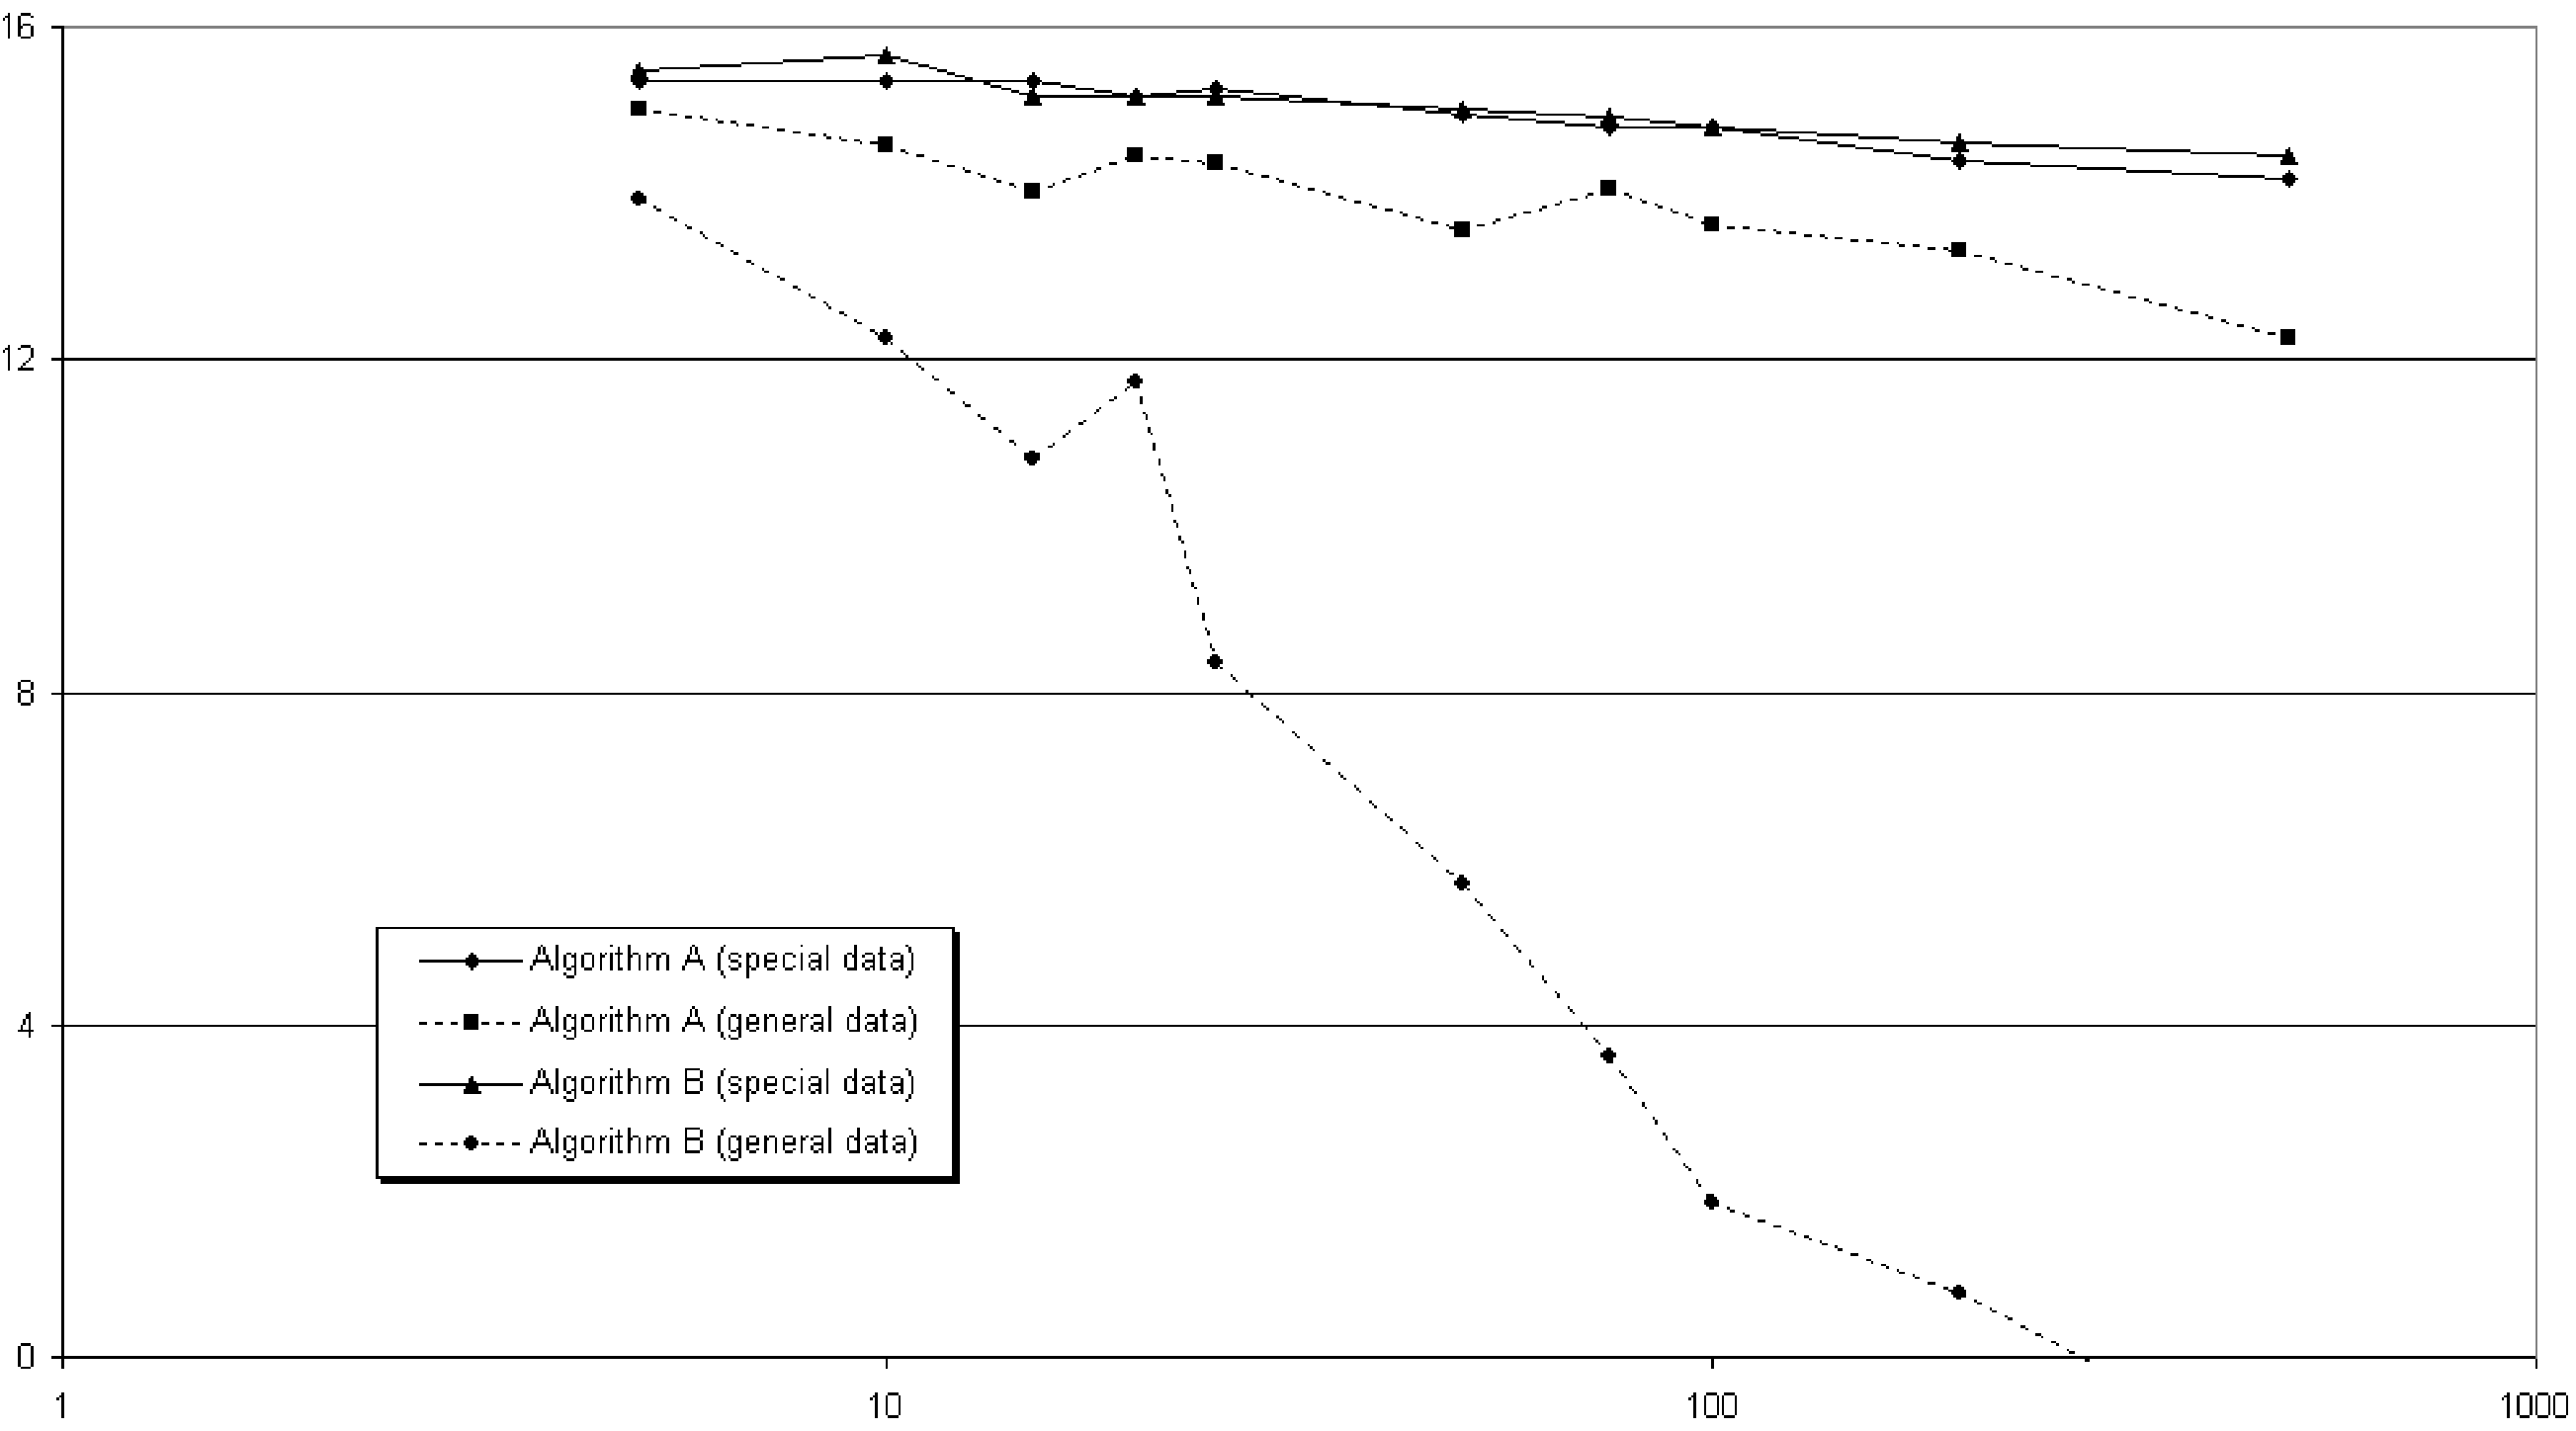
\includegraphics[width=12cm]{Figures/Precision}
\caption{Comparison of achieved precision} \label{fig:precision}
\end{figure}
Figure \ref{fig:precision} shows the results. The parameter
measuring the complexity is laid on the $x$-axis using a
logarithmic scale. The precision is expressed as the negative of
the decimal logarithm of the deviation from the known solution.
The higher the value the better is the precision. The precision of
the floating-point numbers on the machine used in this study
corresponds roughly to 16 on the scale of Figure
\ref{fig:precision}.

The first observation does not come as a surprise: the precision
of each algorithm degrades as the complexity of the problem
increases. One can see that when the algorithms can exploit the
symmetry properties of the data the precision is better (curves
for special data) than for general data. In this case the two
algorithms are performing with essentially the same precision.
Thus, one can chose the faster algorithm, namely algorithm B. For
the general data, however, algorithm B has poorer and poorer
precision as the complexity increases. For complexity larger than
50 algorithm B becomes totally unreliable, to the point of
becoming a perfect illustration of Knuth's quotation above. Thus,
for general data, one has no choice but to use algorithm A.

Readers who do not like mysteries can go read section
\ref{sec:matrixrounding} where these algorithms are discussed.

\subsection{Outsmarting rounding errors}
\label{sec:outsmart} In some instances rounding errors can be
significantly reduced if one spends some time reconsidering how to
compute the final solution. In this section we like to show an
example of such thinking.

Consider the following second order equation, which must be solved
when looking for the eigenvalues of a symmetric matrix (\cf
section \ref{sec:eigensym}):
\begin{equation}
\label{eq:round2nd}
  t^2+2\alpha t - 1 =0.
\end{equation}
Without restricting the generality of the argumentation, we shall
assume that $\alpha$ is positive. the problem is to find the the
root of equation \ref{eq:round2nd} having the smallest absolute
value. You, reader, should have the answer somewhere in one corner
of your brain, left over from high school mathematics:
\begin{equation}
\label{eq:round2ndsol}
  t_{\min}=\sqrt{\alpha^2+1} - \alpha.
\end{equation}
Let us now assume that $\alpha$ is very large, so large that
adding $1$ to $\alpha^2$ cannot be noticed within the machine
precision. Then, the smallest of the solutions of equation
\ref{eq:round2nd} becomes $t_{\min}\approx 0$, which is of course
not true: the left hand side of equation  \ref{eq:round2nd}
evaluates to $-1$.

\noindent Let us now rewrite equation \ref{eq:round2nd} for the
variable $x=1/t$. This gives the following equation:
\begin{equation}
\label{eq:round2ndinv}
  x^2-2\alpha x - 1 =0.
\end{equation}
The smallest of the two solutions of equation \ref{eq:round2nd} is
the largest of the two solutions of equation \ref{eq:round2ndinv}.
That is:
\begin{equation}
  t_{\min}={1\over x_{\max}}={1 \over \sqrt{\alpha^2+1} + \alpha}.
\end{equation}
Now we have for large $\alpha$:
\begin{equation}
  t_{\min}\approx {1\over 2\alpha}.
\end{equation}
This solution has certainly some rounding errors, but much less
than the solution of equation \ref{eq:round2ndsol}: the left hand
side of equation \ref{eq:round2nd} evaluates to ${1\over
4\alpha^2}$, which goes toward zero for large $\alpha$, as it
should be.

\subsection{Wisdom from the past}
To close the subject of rounding errors, I would like to give the
reader a different perspective. There is a big difference between
a full control of rounding errors and giving a result with high
precision. Granted, high precision computation is required to
minimize rounding errors. On the other hand, one only needs to
keep the rounding errors under control to a level up to the
precision required for the final results. There is no need to
determine a result with non-sensical precision.

To illustrate the point, I am going to use a very old mathematical
problem: the determination of the number $\pi$. The story is taken
from the excellent book of Jan Gullberg, {\em Mathematics From the
Birth of the Numbers} \cite{Gullberg}.

Around 300BC, Archimedes devised a simple algorithm to approximate
$\pi$. For a circle of diameter $d$, one computes the perimeter
$p_{\mathop{\textrm in}}$ of a $n$-sided regular polygon inscribed
within the circle and the perimeter $p_{\mathop{\textrm out}}$ of a
$n$-sided regular polygon whose sides the tangent to the same
circle. We have:
\begin{equation}
{\displaystyle p_{\mathop{\textrm in}} \over\displaystyle d
}<\pi<{\displaystyle p_{\mathop{\textrm out}} \over\displaystyle d}.
\end{equation}
By increasing $n$, one can improve the precision of the
determination of $\pi$. During the Antiquity and the Middle Age,
the computation of the perimeters was a formidable task and an
informal competition took place to find who could find the most
precise approximation of the number $\pi$. In 1424, Jamshid Masud
al-Kashi, a persian scientist, published an approximation of $\pi$
with 16 decimal digits. The number of sides of the polygons was
$3\times 2^8$. This was quite an achievement, the last of its
kind. After that, mathematicians discovered other means of
expressing the number $\pi$.

In my eyes, however, Jamshid Masud al-Kashi deserves fame and
admiration for the note added to his publication that places his
result in perspective. He noted that the precision of his
determination of the number $\pi$ was such that,
\begin{quote}{\textit the error
in computing the perimeter of a circle with a radius 600000 times
that of earth would be less than the thickness of a horse's hair}.
\end{quote}
The reader should know that the {\textit thickness of a horse's
hair\/} was a legal unit of measure in ancient Persia
corresponding to roughly 0.7 mm. Using present-day knowledge of
astronomy, the radius of the circle corresponding to the error
quoted by Jamshid Masud al-Kashi is 147 times the distance between
the sun and the earth, or about 3 times the radius of the orbit of
Pluto, the most distant planet of the solar system.

As Jan Gullberg notes in his book, {\textit al-Kashi evidently had a
good understanding of the meaninglessness of long chains of
decimals}. When dealing with numerical precision, you should ask
yourself the following question:
\begin{quote}
{\textsl Do I really need to know the length of Pluto's orbit to a
third of the thickness of a horse's hair?}
\end{quote}

\section{Finding the numerical precision of a computer}
\label{sec:findprecision}
Object-oriented languages such as Smalltalk give the
opportunity to develop an application on one hardware platform and
to deploy the application on other platforms running on different
operating systems and hardware.
It is a well-known fact that the
marketing about Java was centered about the concept of {\textsl Write
Once Run Anywhere}.
What fewer people know is that this concept
already existed for Smalltalk 10 years before the advent of Java.

Some numerical algorithms are carried until the estimated
precision of the result becomes smaller than a given value, called
the desired precision. Since an application can be executing on
different hardware, the desired precision is best determined at
run time.

The book of Press {\textit et al.} \cite{Press} shows a clever code
determining all the parameters of the floating-point
representation of a particular computer. In this book we shall
concentrate only on the parameters which are relevant for
numerical computations. These parameters correspond to the
instance variables of the object responsible to compute them. They
are the following:
\begin{description}
\item[\code{radix}] the radix of the floating-point representation, that is $r$.
\item[\code{machinePrecision}] the largest positive number which, when added to 1 yields 1.
\item[\code{negativeMachinePrecision}] the largest positive number which, when subtracted from 1 yields 1.
\item[\code{smallestNumber}] the smallest positive number different from 0.
\item[\code{largestNumber}] the largest positive number which can be represented in the machine.
\item[\code{defaultNumericalPrecision}] the relative precision, which can be expected for a general numerical computation.
\item[\code{smallNumber}] a number, which can be added to some value without noticeably changing the result of the computation.
\end{description}
Computing the radix $r$ is done in two steps. First one computes a
number equivalent of the machine precision (\cf next paragraph)
assuming the radix is 2. Then, one keeps adding 1 to this number
until the result changes. The number of added ones is the radix.

The machine precision is computed by finding the largest integer
$n$ such that:
\begin{equation}
\left(1+r^{-n}\right)-1\ne 0
\end{equation}
This is done with a loop over $n$. The quantity
$\epsilon_+=r^{-\left(n+1\right)}$ is the machine precision.

The negative machine precision is computed by finding the largest
integer $n$ such that:
\begin{equation}
\left(1-r^{-n}\right)-1\ne 0
\end{equation}
Computation is made as for the machine precision. The quantity
$\epsilon_-=r^{-\left(n+1\right)}$ is the negative machine
precision. If the floating-point representation uses
two-complement to represent negative numbers the machine precision
is larger than the negative machine precision.

To compute the smallest and largest number one first compute a
number whose mantissa is full. Such a number is obtained by
building the expression $f=1-r \times \epsilon_-$. The smallest
number is then computed by repeatedly dividing this value by the
radix until the result produces an underflow. The last value
obtained before an underflow occurs is the smallest number.
Similarly, the largest number is computed by repeatedly
multiplying the value $f$ until an overflow occurs. The last value
obtained before an overflow occurs is the largest number.

The variable \code{defaultNumericalPrecision} contains an estimate
of the precision expected for a general numerical computation. For
example, one should consider that two numbers $a$ and $b$ are
equal if the relative difference between them is less than the
default numerical machine precision. This value of the default
numerical machine precision has been defined as the square root of
the machine precision.

The variable \code{smallNumber} contains a value, which can be
added to some number without noticeably changing the result of the
computation. In general an expression of the type $0 \over 0$ is
undefined. In some particular case, however, one can define a
value based on a limit. For example, the expression $\sin x \over
x $ is equal to 1 for $x=0$. For algorithms, where such an
undefined expression can occur\footnote{Of course, after making
sure that the ratio is well defined numerically.}, adding a small
number to the numerator and the denominator can avoid the division
by zero exception and can obtain the correct value. This value of
the small number has been defined as the square root of the
smallest number that can be represented on the machine.

\subsection{Computer numerical precision}
The computation of the parameters only needs to be executed once.
We have introduced a specific class to hold the variables
described earlier and made them available to any object.

Each parameter is computed using lazy initialization within the
method bearing the same name as the parameter. Lazy initialization
is used while all parameters may not be needed at a given time.
Methods in charge of computing the parameters are all prefixed
with the word compute.

Listing below shows the class \code{PMFloatingPointMachine} responsible of computing the parameters
of the floating-point representation.
This class is implemented as a singleton class because the parameters need to be computed once
only. For that reason no code optimization was made and priority
is given to readability.

\begin{displaycode}{Smalltalk}
Object subclass: #PMFloatingPointMachine
  instanceVariableNames: 'defaultNumericalPrecision radix machinePrecision negativeMachinePrecision smallestNumber largestNumber smallNumber largestExponentArgument'
  classVariableNames: 'UniqueInstance'
  package: 'Math-Core'
\end{displaycode}

\begin{displaycode}{Smalltalk}
PMFloatingPointMachine class >> new
   UniqueInstance = nil
        ifTrue: [ UniqueInstance := super new].
   ^ UniqueInstance
\end{displaycode}

\begin{displaycode}{Smalltalk}
PMFloatingPointMachineMachine >> reset
   UniqueInstance := nil
\end{displaycode}

\noindent The computation of the smallest and largest numbers uses
exceptions to detect the underflow and the overflow.

\begin{displaycode}{Smalltalk}
PMFloatingPointMachine >> computeLargestNumber
    | zero one floatingRadix fullMantissaNumber |
    zero := 0 asFloat.
    one := 1 asFloat.
    floatingRadix := self radix asFloat.
    fullMantissaNumber := one - ( floatingRadix * self negativeMachinePrecision).
    largestNumber := fullMantissaNumber.
    [ [ fullMantissaNumber := fullMantissaNumber * floatingRadix.
        largestNumber := fullMantissaNumber.
        true] whileTrue: [ ].
        ] when: ExAll do: [ :signal | signal exitWith: nil].
\end{displaycode}

\begin{displaycode}{Smalltalk}
PMFloatingPointMachine >> computeMachinePrecision
    | one zero a b inverseRadix tmp x |
    one := 1 asFloat.
    zero := 0 asFloat.
    inverseRadix := one / self radix asFloat.
    machinePrecision := one.
    [ tmp := one + machinePrecision.
      tmp - one = zero]
        whileFalse:[  machinePrecision := machinePrecision * inverseRadix].
\end{displaycode}

\begin{displaycode}{Smalltalk}
PMFloatingPointMachine >> computeNegativeMachinePrecision
    | one zero floatingRadix inverseRadix tmp |
    one := 1 asFloat.
    zero := 0 asFloat.
    floatingRadix := self radix asFloat.
    inverseRadix := one / floatingRadix.
    negativeMachinePrecision := one.
    [ tmp := one - negativeMachinePrecision.
      tmp - one = zero]
        whileFalse: [ negativeMachinePrecision := 
                             negativeMachinePrecision * inverseRadix].
\end{displaycode}

\begin{displaycode}{Smalltalk}
PMFloatingPointMachine >>computeRadix
   | one zero a b tmp1 tmp2 |
   one := 1 asFloat.
   zero := 0 asFloat.
   a := one.
   [ a := a + a.
      tmp1 := a + one.
      tmp2 := tmp1 - a.
      tmp2 - one = zero] whileTrue: [].
    b := one.
    [ b := b + b.
      tmp1 := a + b.
      radix := ( tmp1 - a) truncated.
      radix = 0 ] whileTrue: [].
\end{displaycode}

\begin{displaycode}{Smalltalk}
PMFloatingPointMachine >> computeSmallestNumber
    | zero one floatingRadix inverseRadix fullMantissaNumber |
    zero := 0 asFloat.
    one := 1 asFloat.
    floatingRadix := self radix asFloat.
    inverseRadix := one / floatingRadix.
    fullMantissaNumber := one - ( floatingRadix * self negativeMachinePrecision).
    smallestNumber := fullMantissaNumber.
    [ [ fullMantissaNumber := fullMantissaNumber * inverseRadix.
        smallestNumber := fullMantissaNumber.
        true] whileTrue: [ ].
        ] when: ExAll do: [ :signal | signal exitWith: nil ].
\end{displaycode}

\begin{displaycode}{Smalltalk}
PMFloatingPointMachine >> defaultNumericalPrecision
    defaultNumericalPrecision isNil
        ifTrue: [ defaultNumericalPrecision := self machinePrecision sqrt ].
    ^defaultNumericalPrecision
\end{displaycode}

\begin{displaycode}{Smalltalk}
PMFloatingPointMachine >> largestExponentArgument
    largestExponentArgument isNil
        ifTrue: [ largestExponentArgument := self largestNumber ln].
    ^largestExponentArgument
\end{displaycode}

\begin{displaycode}{Smalltalk}
PMFloatingPointMachine >>largestNumber
    largestNumber isNil
        ifTrue: [ self computeLargestNumber ].
    ^largestNumber
\end{displaycode}

\begin{displaycode}{Smalltalk}
PMFloatingPointMachine >> machinePrecision
    machinePrecision isNil
        ifTrue: [ self computeMachinePrecision ].
    ^machinePrecision
\end{displaycode}

\begin{displaycode}{Smalltalk}
PMFloatingPointMachine >> negativeMachinePrecision
    negativeMachinePrecision isNil
        ifTrue: [ self computeNegativeMachinePrecision ].
    ^negativeMachinePrecision
\end{displaycode}

\begin{displaycode}{Smalltalk}
PMFloatingPointMachine >> radix
    radix isNil
        ifTrue: [ self computeRadix ].
    ^radix
\end{displaycode}

\noindent The method \code{showParameters} can be used to print the
values of the parameters onto the Transcript window.

\begin{displaycode}{Smalltalk}
PMFloatingPointMachine >> showParameters
  Transcript cr; cr;
    nextPutAll: 'Floating-point machine parameters'; cr;
    nextPutAll: '---------------------------------';cr;
    nextPutAll: 'Radix: '.
  self radix printOn: Transcript.
  Transcript cr; nextPutAll: 'Machine precision: '.
  self machinePrecision printOn: Transcript.
  Transcript cr; nextPutAll: 'Negative machine precision: '.
  self negativeMachinePrecision printOn: Transcript.
  Transcript cr; nextPutAll: 'Smallest number: '.
  self smallestNumber printOn: Transcript.
  Transcript cr; nextPutAll: 'Largest number: '.
  self largestNumber printOn: Transcript.
  Transcript flush
\end{displaycode}

\begin{displaycode}{Smalltalk}
PMFloatingPointMachine >> smallestNumber
    smallestNumber isNil
        ifTrue: [ self computeSmallestNumber ].
    ^smallestNumber
\end{displaycode}

\begin{displaycode}{Smalltalk}
PMFloatingPointMachine >> smallNumber
    smallNumber isNil
        ifTrue: [ smallNumber := self smallestNumber sqrt ].
    ^smallNumber
\end{displaycode}

\section{Comparing floating point numbers}
It is very surprising to see how frequently questions about the
lack of equality between two floating-point numbers are posted on
the Smalltalk electronic discussion groups. As we have
seen in section \ref{sec-rounding} one should always expect the
result of two different computations that should have yielded the
same number from a mathematical standpoint to be different using a
finite  numerical representation. Somehow the computer courses are
not giving enough emphasis about floating-point numbers.

\begin{quote}
So, how should you check the equality of two floating-point
numbers? The practical answer is: {\textsl thou shalt not!}
\end{quote}

\noindent As you will see, the algorithms in this book only
compare numbers, but never check for equality. If you cannot
escape the need for a test of equality, however, the best solution
is to create methods to do this. Since the floating-point
representation is keeping a constant relative precision,
comparison must be made using relative error. Let $a$ and $b$ be
the two numbers to be compared. One should build the following
expression:
\begin{equation}
\label{eq:relerror}
\epsilon={\left|a-b\right| \over
\max\left(\left|a\right|,\left|b\right|\right)}
\end{equation}
The two numbers can be considered equal if $\epsilon$ is smaller
than a given number $\epsilon_{\max}$. If the denominator of the
fraction on equation \ref{eq:relerror} is less than
$\epsilon_{\max}$, than the two numbers can be considered as being
equal. For lack of information on how the numbers $a$ and $b$ have
been obtained, one uses for $\epsilon_{\max}$ the default
numerical precision defined in section \ref{sec:findprecision}.
If one can determine the precision of each number, then the method \code{relativelyEqual} can be used.

In Smalltalk this means adding a new method to the class Number as
shown in Listing \ref{lst:fltcompare}.

\begin{listing}[label=lst:fltcompare]{Smalltalk}
{Comparison of floating point numbers in Smalltalk}
Number >> equalsTo: aNumber
   ^self relativelyEqualsTo: aNumber upTo:
         PMFloatingPointMachine new defaultNumericalPrecision
\end{listing}

\begin{displaycode}{Smalltalk}
Number >> relativelyEqualsTo: aNumber upTo: aSmallNumber
   | norm |
   norm := self abs max: aNumber abs.
   ^norm <= PMFloatingPointMachine new defaultNumericalPrecision
    or: [ (self - aNumber) abs < ( aSmallNumber * norm)]
\end{displaycode}

\section{Speed consideration (to be revisited)}
\label{sec:speed} Some people may think that implementing
numerical methods for object-oriented languages such as Smalltalk just a waste
of time. Those languages are notoriously slow or so they think.

First of all, things should be put in perspective with other
actions performed by the computer. If a computation does not take
longer than the time needed to refresh a screen, it does not
really matter if the application is interactive. For example,
performing a least square fit to a histogram in Smalltalk and drawing the
resulting fitted function is usually hardly perceptible to the eye on a personal
computer. Thus, even though a C version runs 10 times faster, it
does not make any difference for the end user. The main difference
comes, however, when you need to modify the code. Object-oriented
software is well known for its maintainability. As $80\%$ of the
code development is spent in maintenance this aspect should first
be considered.

Table \ref{tb:speed} shows measured speed of execution for some of
the algorithms exposed in this book. Timing was done on a personal
computer equipped with a Pentium II clocked at 200MHz and running
Windows NT workstation 4.0. The C code used is the code of
\cite{Press} compiled with the C compiler Visual C$^{++}$ 4.0 from
Microsoft Corporation. The time needed to allocate memory for
intermediate results was included in the measurement of the C
code, otherwise the comparison with object-oriented code would not
be fair. The Smalltalk code was run under version 4.0 of Visual
Age\tm for Smalltalk from IBM Corporation using the ENVY benchmark
tool provided.
Elapsed time were measured
by repeating the measured evaluation a sufficient number of time
so that the error caused by the CPU clock is less that the last
digit shown in the final result.
\begin{table}[h]
\caption{Compared execution speed between C and Smalltalk}
\label{tb:speed} \vspace{1 ex}
\begin{tabular}{|l | c r r |} \hline
  \hfil {\textbf Operation} & {\textbf Units} & {\textbf C}\hfil & {\textbf Smalltalk}\hfil \\ \hline
  Polynomial $10\th$ degree & msec. & 1.1 & 27.7 \\
  Neville interpolation (20 points) & msec. & 0.9 & 11.0 \\
  LUP matrix inversion ($100\times 100$)& sec. & 3.9 & 22.9 \\ \hline
\end{tabular}
\end{table}

One can see that object-oriented code is quite efficient,
especially when it comes to complex algorithms: good
object-oriented code can actually beat up C code.

%My early tests with Java, a couple of years ago, were showing that
%Java was 5-10 times slower than C. One can see that vendors did a
%great job in optimizing the generated code and in accelerating the
%virtual machine. I would like to see the same efforts going in
%optimizing Smalltalk. The spectacular improvement of Java shows
%that it is possible. Actually, my early tests made with Visual
%Smalltalk\tm from Digitalk Inc.\footnote{Unfortunately, the future
%of Visual Smalltalk now owned by Cincom Inc. is quite uncertain at
%this time of writing.} were 5 times better.

%Today admittedly, I would not use Smalltalk to build a structural
%analysis program, but Java would certainly be a contender.
I have successfully build data mining Smalltalk
applications using {\textbf all the code}\footnote{I want to emphasize
here that all the code of this book is real code, which I have
used personally in real applications.} presented in this book.
These applications were not perceived as slow by the end user
since most of the computer time was spent drawing the data.

\subsection{Smalltalk particular}
Smalltalk has an interesting property: a division between two
integers is by default kept as a fraction. This prevents rounding
errors. For example, the multiplication of a matrix of integer
numbers with its inverse always yields an exact identity matrix.
(\cf section \ref{sec:lup} for definitions of these terms).

There is, however, a price to pay for the perfection offered by
fractions. When using fractions, the computing time often becomes
prohibitive. Resulting fractions are often composed of large
integers. This slows down the computing. In the case of matrix
inversion, this results in an increase in computing time by
several orders of magnitude.

For example, one of my customers was inverting a $301\times 301$
matrix with the code of section \ref{sec:lup}. The numbers used to
build the matrix where obtained from a measuring device (using an
ADC) and where thus integers. The inversion time was over 2
hours\footnote{This particular customer was a {\textsl very} patient
person!}. After converting the matrix components to floating
numbers the inversion time became less than 30 seconds!

If you are especially unlucky you may run out of memory when
attempting to store a particularly long integer. Thus, it is
always a good idea to use floating\footnote{In most available
Smalltalk versions the class Float corresponds to floating numbers
with double precision. VisualWorks makes the difference between
\code{Float} and \code{Double}} numbers instead of fractions unless
absolute accuracy is your primary goal. My experience has been
that using floating numbers speeds up the computation by at least
an order of magnitude.
In the case of complex computations such as
matrix inversion or least square fit this can become prohibitive.

\section{Conventions}
Equations presented in this book are using standard international
mathematical notation as described in \cite{Knuth1}. Each section
is trying to made a quick derivation of the concepts needed to
fully understand the mathematics behind the scene. For readers in
a hurry, the equations used by the implementation are flagged as
the following sample equation:
\begin{mainEquation}
\ln ab = \ln a + \ln b.
\end{mainEquation}
When such an equation is encountered, the reader is sure that the
expression is implemented in the code.

In general the code presented in this book adheres to conventions
widely used in each language. Having said that, there are a few
instances where we have departed from the widely used conventions.

\subsection{Class diagrams}
When appropriate a class diagram is shown at the beginning of each
chapter. This diagram shows the hierarchy of the classes described
in the chapter and eventually the relations with classes of other
chapters. The diagrams are drawn using the conventions of the book
on design patterns \cite{GoF}.

Figure \ref{fig:classDiagram} shows a typical class diagram. A
rectangular box with 2 or 3 parts represents a class. The top part
contains the name of the class in bold face. If the class is an
abstract class the name in shown in italic bold face.
In figure \ref{fig:classDiagram} the classes \code{RelatedClass}, \code{MySubClass1} and \code{MySubclass2} are concrete classes; \code{MyAbstractClass} is an abstract class.
The second part of the class box contains a list of the public instance methods.
The name of an abstract method is written in italic, for example \code{abstractMethod3} in the class \code{MyAbstractClass} of figure \ref{fig:classDiagram}.
The third part of the class box, if any, contains the list of all instance variables.
If the class does not
have any instance variable the class box only consists of 2 parts,
for example the class \code{MySubClass1} of figure
\ref{fig:classDiagram}.
\begin{figure}
\centering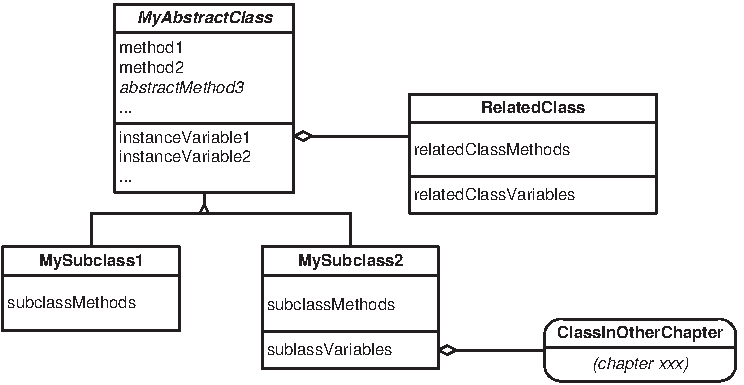
\includegraphics[width=11cm]{Figures/TypicalClassDiagram}
\caption{A typical class diagram} \label{fig:classDiagram}
\end{figure}

A vertical line with a triangle indicates class inheritance. If
there are several subclasses the line branches at the triangle, as
this is the case in figure \ref{fig:classDiagram}. A horizontal
line beginning with a diamond (UML aggregation symbol) indicates
the class of an instance variable. For example, Figure
\ref{fig:classDiagram} indicates that the instance variable \code{instanceVariable1} of the class \code{MyAbstractClass} must be an
instance of the class \code{RelatedClass}. The diamond is black is
the instance variable is a collection of instances of the class. A
class within a rectangle with rounded corner represents a class
already discussed in an earlier chapter; the reference to the
chapter is written below the class name. Class \code{ClassInOtherChapter} in figure \ref{fig:classDiagram} is such a
class. To save space, we have used the
Smalltalk method names. It is quite easy to identify methods
needing parameters when one uses Smalltalk method names: a
colon in the middle or at the end of the method name indicates
a parameter. Please refer to appendix \ref{ch:smalltalkprimer} for
more details on Smalltalk methods.

\subsection{Smalltalk code}
Most of the Smalltalk systems do not support name spaces. As a
consequence, it has becomed a convention to prefix all class names
with 3-letter code identifying the origin of the code. In this
book the names of the Smalltalk classes are all prefixed with PM like PolyMath\footnote{Classes were previously prefixed with author's initials.}.

There are several ways to store constants needed by all instances
of a class. One way is to store the constants in class variables.
This requires each class to implement an initialization method,
which sets the desired values into the class variables. Another
way is to store the constants in a pool dictionary. Here also an
initialization method is required. In my opinion pool dictionaries
are best used for texts, as they provide a convenient way to
change all text from one language to another. Sometimes the
creation of a singleton object is used. This is especially useful
when the constants are installation specific and, therefore, must
be determined at the beginning of the application's execution,
such as the precision of the machine (\cf section
\ref{sec:findprecision}). Finally constants which are not likely
to change can be stored in the code. This is acceptable as long as
this is done at a unique place. In this book most constants are
defined in class methods.

By default a Smalltalk method returns \code{self}. For
initialization methods, however, we write this return explicitly
(\code{^self}) to ease reading. This adheres to the intention
revealing patterns of Kent Beck \cite{Beck}.

In \cite{StDesPat} it is recommended to use the method name \code{default} to implement a singleton class. In this book this
convention is not followed. In Smalltalk, however, the normal
instance creation method is \code{new}. Introducing a method \code{default} for singleton classes has the effect of departing from
this more ancient convention. In fact, requiring the use of \code{default} amounts to reveal to the client the details of
implementation used by the class. This is in clear contradiction
with the principle of hiding the implementation to the external
world.
Thus, singleton classes in all code presented in this book
are obtained by sending the method \code{new} to the class.
A method named \code{default} is reserved for the very semantic of
the word default: the instance returned by these methods is an
instance initialized with some default contents, well specified.
Whether or not the instance is a singleton is not the problem of
the client application.

\section{Roadmap}
This last section of the introduction describes the roadmap of
the algorithms discussed in the book chapter by chapter. Figure
\ref{fig:roadmap} shows a schematic view of the major classes
discussed in this book together with their dependency relations.
\begin{figure}
\centering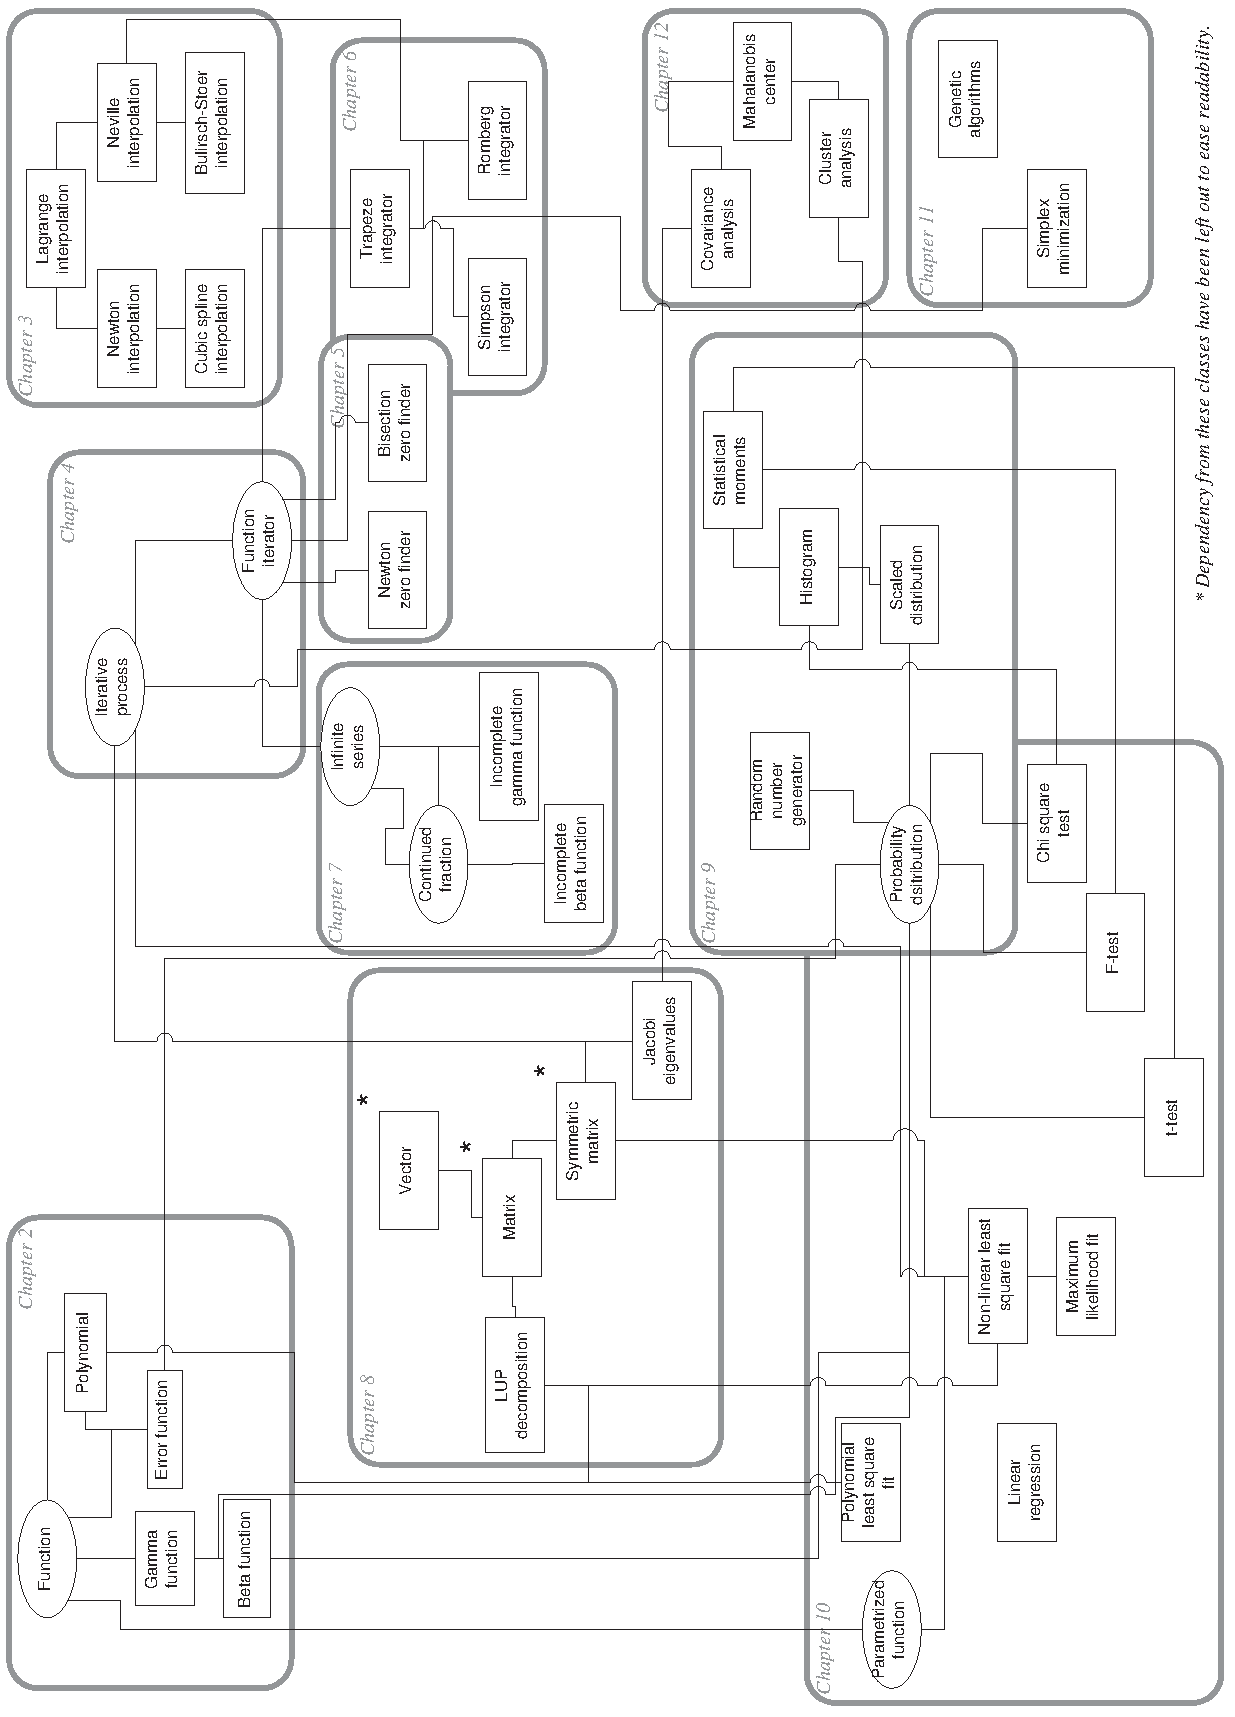
\includegraphics[width=13cm]{Figures/Roadmap}
\caption{Book roadmap} \label{fig:roadmap}
\end{figure}
In this figure, abstract classes are represented with an ellipse,
concrete classes with a rectangle. Dependencies between the
classes are represented by lines going from one class to another;
the dependent class is always located below. Chapters where the
classes are discussed are drawn as grayed rectangles with rounded
corners. Hopefully the reader will not be scared by the complexity
of the figure. Actually, the figure should be more complex as the
classes \code{Vector} and \code{Matrix} are used by most objects
located in chapters \ref{ch:linearalgebra} and following. To
preserve the readability of figure \ref{fig:roadmap} the
dependency connections for these two classes have been left out.

Chapter \ref{ch:function} presents a general representation of
mathematical functions. Examples are shown. A concrete
implementation of polynomial is discussed. Finally three library
functions are given: the error function, the gamma function and
the beta function.

Chapter \ref{ch:interpolation} discusses interpolation algorithms.
A discussion explains when interpolation should be used and which
algorithm is more appropriate to which data.

Chapter \ref{ch:iteration} presents a general framework for
iterative process. It also discusses a specialization of the
framework to iterative process with a single numerical result.
This framework is widely used in the rest of the book.

Chapter \ref{ch:zeroes} discusses two algorithms to find the
zeroes of a function: bisection and Newton's zero finding
algorithms. Both algorithms use the general framework of chapter
\ref{ch:iteration}.

Chapter \ref{ch:integration} discusses several algorithms to
compute the integral of a function. All algorithms are based on
the general framework of chapter \ref{ch:iteration}. This chapter
also uses an interpolation technique from chapter
\ref{ch:interpolation}.

Chapter \ref{ch:series} discusses the specialization of the
general framework of chapter \ref{ch:iteration} to the computation
of infinite series and continued fractions. The incomplete gamma
function and incomplete beta function are used as concrete
examples to illustrate the technique.

Chapter \ref{ch:linearalgebra} presents a concrete implementation
of vector and matrix algebra. It also discusses algorithms to
solve systems of linear equations. Algorithms to compute matrix
inversion and the finding of eigenvalues and eigenvectors are
exposed. Elements of this chapter are used in other part of this
book.

Chapter \ref{ch:statistics} presents tools to perform statistical
analysis. Random number generators are discussed. We give an
abstract implementation of a probability distribution with
concrete example of the most important distributions. The
implementation of other distributions is given in appendix. This
chapter uses techniques from chapters \ref{ch:function},
\ref{ch:zeroes} and \ref{ch:integration}.

Chapter \ref{ch:estimation} discussed the test of hypothesis and
estimation. It gives an implementation of the t- and F-tests. It
presents a general framework to implement least square fit and
maximum likelihood estimation. Concrete implementations of least
square fit for linear and polynomial dependence are given. A
concrete implementation of the maximum likelihood estimation is
given to fit a probability distribution to a histogram. This
chapter uses techniques from chapter \ref{ch:function},
\ref{ch:iteration}, \ref{ch:linearalgebra} and
\ref{ch:statistics}.

Chapter \ref{ch:minimization} discusses some techniques used to
maximize or minimize a function: classical algorithms (simplex,
hill climbing) as well as new ones (genetic algorithms). All these
algorithms are using the general framework for iterative process
discussed in chapter \ref{ch:iteration}.

Chapter \ref{ch:datamining} discusses the modern data mining
techniques: correlation analysis, cluster analysis and neural
networks. A couple of methods invented by the author are also
discussed. This chapter uses directly or indirectly techniques
from all chapters of this book.

%\ifx\wholebook\relax\else\end{document}\fi

%\ifx\wholebook\relax\else
%\documentclass[twoside]{book}
%\usepackage[active]{srcltx}
%\usepackage[LY1]{fontenc}
%\usepackage{url}
\makeatletter
\def\url@leostyle{%
  \@ifundefined{selectfont}{\def\UrlFont{\sf}}{\def\UrlFont{\sffamily}}}
\makeatother
% Now actually use the newly defined style.
\urlstyle{leo}

\usepackage{graphicx}
\def\etc{{\textit{etc}}}
\def\eg{{\textit{e.g.}}}
\def\ie{{\textit{i.e.}}}
\def\cf{{\textit{c.f.}}\ }
\def\erf{\mathop{\textrm{erf}}}
\def\sign{\mathop{\textrm{sign}}}
\def\prob{\mathop{\textrm{Prob}}}
\def\var{\mathop{\textrm{var}}}
\def\mod{\mathop{\textrm{mod}}}
\def\cor{\mathop{\textrm{cor}}}
\def\cov{\mathop{\textrm{cov}}}
\def\cl{\mathop{\textrm{CL}}}
\def\kg{\mathop{\textrm{Kg}}}
\def\patstyle#1{{\textsc #1}}
\def\th{^{\mathop{\textrm{th}}}}
%\def\st#1{^{\mathop{\rm #1}}}
\def\note#1{\begin{quote}{\textbf{Note:}} #1\end{quote}}
\def\braket#1{\left\langle #1\right\rangle}
\def\order#1{\let\o=#1$\mathcal{O}$\ifx\o 1$\left(n\right)$\else$\left(n^{#1}\right)$\fi}
%\newtheorem{privListing}{Listing}[chapter]
%\newenvironment{listing}{\vskip 3ex\hrule\vskip 1ex\begin{privListing}}{\end{privListing}\hrule\vskip 1ex}
\newtheorem{privExample}{Code example}[chapter]
\newenvironment{codeExample}{\begin{privExample}\begin{quote}\tt}{\end{quote}\end{privExample}}
\def\relboxl#1#2{\hbox to #1\hsize{#2\hfil}}
\def\relboxc#1#2{\hbox to #1\hsize{\hfil #2\hfil}}
\def\relboxr#1#2{\hbox to #1\hsize{\hfil #2}}
\def\transpose#1{\textbf{#1}^{\mathop\textrm{T}}}
\def\inverse#1{\textbf{#1}^{-1}}
%\def\tm{$^{\mathop{\rm TM}}$}
\def\tm{ }
\newenvironment{mainEquation}{\marginpar[\vspace{3 ex} Main
equation$\Rightarrow$]{\vspace{3 ex}$\Leftarrow$Main
equation}\begin{equation}}{\end{equation}}
\def\rubrique#1{\paragraph{#1}\hfil\par\noindent}

%\begin{document}
%\fi

\chapter{Function evaluation}
\label{ch:function} \vspace{1 ex}
\begin{flushright}
{\textsl Qu'il n'y ait pas de r\'eponse n'excuse pas l'absence de
questions.}\footnote{The absence of answer does not justify the
absence of question.}\\ Claude Roy
\end{flushright}
\vspace{1 ex} Many mathematical functions used in numerical
computation are defined by an integral, by a recurrence formula or
by a series expansion. While such definitions can be useful to a
mathematician, they are usually quite complicated to implement on
a computer. For one, not every programmer knows how to evaluate an
integral numerically\footnote{The good news is that they will if
they read the present book (\cf chapter \ref{ch:integration}).}.
Then, there is the problem of accuracy. Finally, the evaluation of
the function as defined mathematically is often too slow to be
practical.

Before computers were heavily used, however, people had already
found efficient ways of evaluating complicated functions. These
methods are usually precise enough and extremely fast. This
chapter exposes several functions that are important for
statistical analysis. The Handbook of Mathematical Functions by
Abramovitz and Stegun \cite{AbrSteg} contains a wealth of such
function definitions and describes many ways of evaluating them
numerically. Most approximations used in this chapter have been
taken from this book.

This chapter opens on general considerations on how to implement
the concept of function. Then, polynomials are discussed as an
example of concrete function implementation. The rest of this
chapter introduces three classical functions: the error function,
the gamma function and the beta function. We shall use this
functions in chapters \ref{ch:statistics} and \ref{ch:estimation}.
Because these functions are fundamental functions used in many
areas of mathematics they are implemented as library functions ---
such as a sine, log or exponential --- instead of using the
general function formalism described in the first section.

Figure \ref{fig:functions} shows the diagram of the Smalltalk classes
described in this chapter.
\begin{figure}
\centering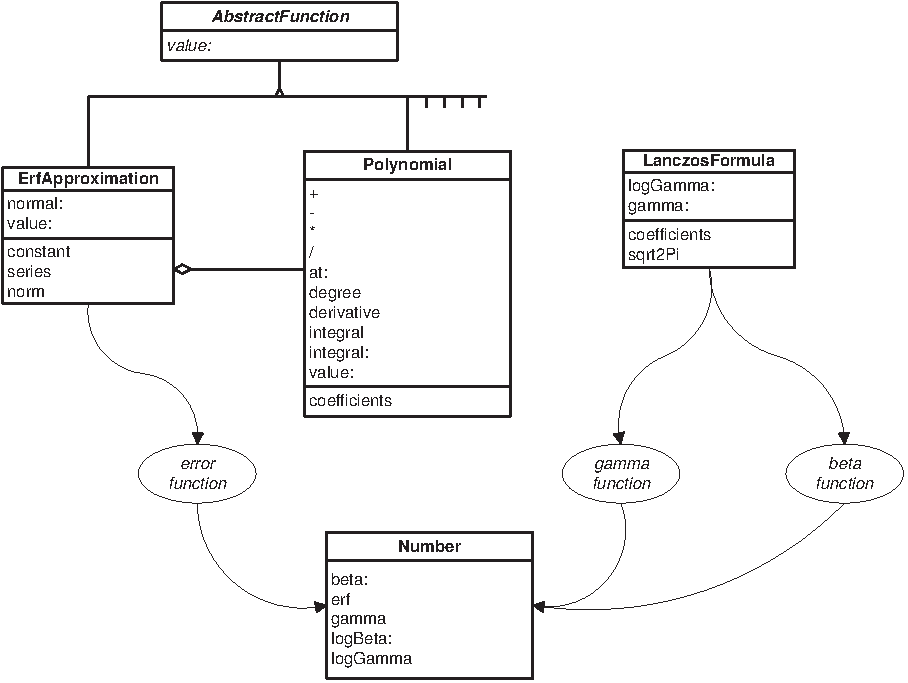
\includegraphics[width=10cm]{Figures/FunctionS}
\caption{Smalltalk classes related to functions}
\label{fig:functions}
\end{figure}
Here we have used special notations to indicate that the functions
are implemented as library functions. The functions are
represented by oval and arrows shows which class is used to
implement a function for the class \code{Number}.

\section{Function concept}
\label{sec:function}
A mathematical function is an object
associating a value to a variable. If the variable is a single
value one talks about a one variable function. If the variable is
an array of values one talks about a multi-variable function.
Other types of variables are possible but will not be covered in
this book.

We shall assume that the reader is familiar with elementary
concepts about functions, namely derivatives and integrals. We
shall concentrate mostly on implementation issues.

\section{Function -- Smalltalk implementation}
\label{sec:stFunction}
A mathematical function is an object
associating a value to a variable. If the variable is a single
value one talks about a one variable function. If the variable is
an array of values one talks about a multi-variable function.
Other types of variables are possible but will not be covered in
this book.

We shall assume that the reader is familiar with elementary
concepts about functions, namely derivatives and integrals. We
shall concentrate mostly on implementation issues.

\marginpar{Figure \ref{fig:functions} with
the box \code{AbstractFunction} grayed.} A function in Smalltalk
can be readily implemented with a block closure. Block closures in
Smalltalk are treated like objects; thus, they can be manipulated
as any other objects. For example the one variable function
defined as:
\begin{equation}
f\left( x \right)={1 \over x},
\end{equation}
can be implemented in Smalltalk as:
\begin{displaycode}{Smalltalk}
f := [:x | 1 / x].
\end{displaycode}
Evaluation of a block closure is supplied by the method value:.
For example, to compute the inverse of 3, one writes:
\begin{displaycode}{Smalltalk}
f value: 3.
\end{displaycode}

If the function is more complex a block closure may not be the
best solution to implement a function. Instead a class can be
created with some instance variables to hold any constants and/or
partial results. In order to be able to use functions
indifferently implemented as block closures or as classes, one
uses polymorphism. Each class implementing a function must
implement a method \code{value:}.
Thus, any object evaluating a function can send the same message selector, namely \code{value:}, to the variable
holding the function.

To evaluate a multi-variable function, the argument of the method
\code{value:} is an Array or a vector (\cf section
\ref{sec:linearalgebra}). Thus, in Smalltalk multi-variable
functions can follow the same polymorphism as for one-variable
functions.

\section{Polynomials}
\label{sec:polynomial}
 Polynomials are quite important in
numerical methods because they are often used in approximating
functions. For example, section \ref{sec:errorFunction} shows how
the error function can be approximated with the product of normal
distribution times a polynomial.

Polynomials are also useful in approximating functions, which are
determined by experimental measurements in the absence of any
theory on the nature of the function. For example, the output of a
sensor detecting a coin is dependent on the temperature of the
coin mechanism. This temperature dependence cannot be predicted
theoretically because it is a difficult problem. Instead, one can
measure the sensor output at various controlled temperatures.
These measurements are used to determine the coefficients of a
polynomial reproducing the measured temperature variations. The
determination of the coefficients is performed using a polynomial
least-square fit (\cf section \ref{sec:lsfpol}). Using this
polynomial the correction for a given temperature can be evaluated
for any temperature within the measured range.

The reader is advised to read carefully the implementation section as many techniques are introduced at this occasion.
Later on those techniques will be mentioned with no further explanations.

\subsection{Mathematical definitions}
\label{sec:polymath} A polynomial is a special mathematical
function whose value is computed as follows:
\begin{equation}
\label{eq:polynomialDef}P\left(x\right)=\sum_{k=0}^{n}a_k x^k.
\end{equation}
$n$ is called the degree of the polynomial. For example, the
second order polynomial
\begin{equation}
\label{eq:polynomialExample} x^2 -3x + 2
\end{equation}
represents a parabola crossing the $x$-axis at points 1 and 2 and
having a minimum at $x= 2/3$. The value of the polynomial at the
minimum is $-1/4$.

In equation \ref{eq:polynomialDef} the numbers $a_0, \ldots a_n$
are called the coefficients of the polynomial. Thus, a polynomial
can be represented by the array $\left\{ a_0, \ldots a_n
\right\}$. For example, the polynomial of equation
\ref{eq:polynomialExample} is represented by the array $\left\{
2,-3,1 \right\}$.

Evaluating equation \ref{eq:polynomialDef} as such is highly
inefficient since one must raise the variable to an integral power
at each term. The required number of multiplication is of the
order of $n^2$. There is of course a better way to evaluate a
polynomial. It consists of factoring out $x$ before the evaluation
of each term\footnote{This is actually the first program I ever
wrote in my first computer programming class. Back in 1969, the
language in fashion was ALGOL.}. The following formula shows the
resulting expression:
\begin{mainEquation}
\label{eq:horner}
\left(x\right)=a_0+x\left\{a_1+x\left[a_2+x\left(a_3+\cdots\right)\right]\right\}
\end{mainEquation}
Evaluating the above expression now requires only multiplications.
The resulting algorithm is quite straightforward to implement.
Expression \ref{eq:horner} is called Horner's rule because it was
first published by W.G. Horner in 1819. 150 years earlier,
however, Isaac Newton was already using this method to evaluate
polynomials.

In section \ref{sec:newton} we shall requires the derivative of a
function. For polynomials this is rather straightforward. The
derivative is given by:
\begin{equation}
\label{eq:polynomialDeriv}{dP\left(x\right)\over
dx}=\sum_{k=1}^{n}k a_k x^{k-1}.
\end{equation}
Thus, the derivative of a polynomial with $n$ coefficients is
another polynomial, with $n-1$ coefficients\footnote{Notice the
change in the range of the summation index in equation
\ref{eq:polynomialDeriv}.} derived from the coefficients of the
original polynomial as follows:
\begin{equation}
a^\prime _k=\left(k+1\right)a_{k+1}\mbox{\quad for
$k=0,\ldots,n-1$}.
\end{equation}
For example, the derivative of \ref{eq:polynomialExample} is
$2x-3$.

The integral of a polynomial is given by:
\begin{equation}
\int_0^xP\left(t\right)dt=\sum_{k=0}^{n}{a_k \over k+1} x^{k+1}.
\end{equation}
Thus, the integral of a polynomial with $n$ coefficients is
another polynomial, with $n+1$  coefficients derived from the
coefficients of the original polynomial as follows:
\begin{equation}
\bar{a}_k={a_{k-1}\over k}\mbox{\quad for $k=1,\ldots,n+1$}.
\end{equation}
For the integral, the coefficient $\bar{a}_0$ is arbitrary and
represents the value of the integral at $x=0$. For example the
integral of \ref{eq:polynomialExample} which has the value -2 at
$x=0$ is the polynomial
\begin{equation}
{x^3\over 3}-{3 ^2\over2}+2x-2.
\end{equation}
Conventional arithmetic operations are also defined on polynomials
and have the same properties\footnote{The set of polynomials is a
vector space in addition to being a ring.} as for signed integers.

Adding or subtracting two polynomials yields a polynomial whose
degree is the maximum of the degrees of the two polynomials. The
coefficients of the new polynomial are simply the addition or
subtraction of the coefficients of same order.

Multiplying two polynomials yields a polynomial whose degree is
the product of the degrees of the two polynomials. If $\left\{
a_0,\ldots,a_n \right\}$ and $\left\{ b_0,\ldots,b_n \right\}$ are
the coefficients of two polynomials, the coefficients of the
product polynomial are given by:
\begin{equation}
\label{eq:polMult} c_k = \sum_{i+j=k}a_i b_j \mbox{\quad for
$k=0,\ldots,n+m$}.
\end{equation}
In equation \ref{eq:polMult} the coefficients $a_k$ are treated as
0 if $k>n$. Similarly the coefficients $n_k$ are treated as 0 if
$k>m$.

Dividing a polynomial by another is akin to integer division with
remainder. In other word the following equation:
\begin{equation}
P\left(x\right)=Q\left(x\right)\cdot
T\left(x\right)+R\left(x\right).
\end{equation}
uniquely defines the two polynomials $Q\left(x\right)$, the
quotient, and $R\left(x\right)$, the remainder, for any two given
polynomials $P\left(x\right)$ and $T\left(x\right)$. The algorithm
is similar to the algorithm taught in elementary school for
dividing integers \cite{Knuth2}.

\subsection{Polynomial --- Smalltalk implementation}
As we have seen a polynomial is uniquely defined by its
coefficients. Thus, the creation of a new polynomial instance must
have the coefficients given. Our implementation assumes that the
first element of the array containing the coefficients is the
coefficient of the constant term, the second element the
coefficient of the linear term ($x$), and so on.

The method \code{value} evaluates the polynomial at the supplied
argument. This methods implements equation \ref{eq:horner}.

The methods \code{derivative} and \code{integral} return each a new
instance of a polynomial. The method \code{integral:} must have an
argument specifying the value of the integral of the polynomial at
0. A convenience \code{integral} method without a<rgument is
equivalent to call the method \code{integral} with argument 0.

The implementation of polynomial arithmetic is rarely used in
numerical computation though. It is, however, a nice example to
illustrate a technique called double dispatching. Double
dispatching is described in appendix (\cf section
\ref{sec:doubledisp}). The need for double dispatching comes for
allowing an operation between object of different nature. In the
case of polynomials operations can be defined between two
polynomials or between a number and a polynomial. In short, double
dispatching allows one to identify the correct method based on the
type of the two arguments.

\marginpar{Figure \ref{fig:functions}
with the box {\textbf Polynomial} grayed.}
Being a special case of a function a polynomial must of course implement the behavior of
functions as discussed in section \ref{sec:stFunction}.
Here is a code example on how to use the class \code{PMPolynomial}.
\begin{listing}{Smalltalk}
{How to use PMPolynomial}
| polynomial |
polynomial := PMPolynomial coefficients: #(2 -3 1).
polynomial value: 1.
\end{listing}
The code above creates an instance of the class \code{PMPolynomial} by giving the coefficient of the polynomial. In
this example the polynomial $x^2-3x+2$. The final line of the code
computes the value of the polynomial at $x=1$.

The next example shows how to manipulate polynomials in symbolic form.
\begin{listing}{Smalltalk}
{ }
| pol1 pol2 polynomial polD polI |
pol1:= PMPolynomial coefficients: #(2 -3 1).
pol2:= PMPolynomial coefficients: #(-3 7 2 1).
polynomial := pol1 * pol2.
polD := polynomial derivative.
polI := polynomial integral.
\end{listing}
The first line creates the  polynomial of example
\ref{eq:polynomialExample}. The second line creates the polynomial
$x^3+2x^2+7x-3$. The third line of the code creates a new
polynomial, product of the first two. The last two lines create
two polynomials, respectively the derivative and the integral of
the polynomial created in the third line.

Listing \ref{ls:polynomial} shows the Smalltalk implementation of
the class \code{PMPolynomial}.

A beginner may have been tempted to make \code{PMPolynomial} a subclass of \code{Array} to spare the need for an instance variable.
This is of course quite wrong.
An array is a subclass of \code{Collection}.
Most methods implemented or inherited by \code{Array} have nothing to do with the behavior of a polynomial as a mathematical entity.

Thus, a good choice is to make the class \code{PMPolynomial} a
subclass of Object. It has a single instance variable, an Array
containing the coefficients of the polynomial.

It is always a good idea to implement a method \code{printOn:} for
each class. This method is used by many system utilities to
display an object in readable form, in particular the debugger and
the inspectors. The standard method defined for all objects simply
displays the name of the class. Thus, it is hard to decide if two
different variables are pointing to the same object. Implementing
a method \code{printOn:} allows displaying parameters particular to
each instance so that the instances can easily be identified. It
may also be used in quick print on the \code{Transcript} and may
save you the use on an inspector while debugging. Implementing a
method \code{printOn:} for each class that you create is a good
general practice, which can make your life as a Smalltalker much
easier.

Working with indices in Smalltalk is somewhat awkward for
mathematical formulas because the code is quite verbose. In
addition a mathematician using Smalltalk for the first time may be
disconcerted with all indices starting at 1 instead of 0.
Smalltalk, however, has very powerful iteration methods, which
largely compensate for the odd index choice, odd for a
mathematician that is. In fact, an experienced Smalltalker seldom
uses indices explicitly as Smalltalk provides powerful iterator
methods.

The method \code{value:} uses the Smalltalk iteration method \code{inject:into:} (\cf section \ref{sec:injectinto}). Using this
method requires storing the coefficients in reverse order because
the first element fed into the method \code{inject:into:}
corresponds to the coefficient of the largest power of $x$. It
would certainly be quite inefficient to reverse the order of the
coefficients at each evaluation. Since this requirement also
simplifies the computation of the coefficients of the derivative
and of the integral, reversing of the coefficients is done in the
creation method to make things transparent.

The methods \code{derivative} and \code{integral} return a new
instance of the class \code{PMPolynomial}. They do not modify the
object receiving the message. This is also true for all operations
between polynomials. The methods \code{derivative} and \code{integral} use the method \code{collect:} returning a collection of
the values returned by the supplied block closure at each argument
(\cf section \ref{sec:collect}).

The method \code{at:} allows one to retrieve a given coefficient.
To ease readability of the multiplication and division methods,
the method \code{at:} has been defined to allow for indices
starting at 0. In addition this method returns zero for any index
larger than the polynomial's degree. This allows being lax with
the index range. In particular, equation \ref{eq:polMult} can be
coded exactly as it is.

The arithmetic operations between polynomials are implemented
using double dispatching. This is a general technique widely used
in Smalltalk (and all other languages with dynamical typing)
consisting of selecting the proper method based on the type of the
supplied arguments. Double dispatching is explained in section
\ref{sec:doubledisp}.

\note{Because Smalltalk is a dynamically typed language, our
implementation of polynomial is also valid for polynomials with
complex coefficients.}

\begin{listing}[label=lst:polynomial]{Smalltalk}
{Smalltalk implementation of the polynomial class}
Object subclass: #PMPolynomial
   instanceVariableNames: 'coefficients'
   classVariableNames: ''
   package: 'Math-Polynomials'
\end{listing}

\begin{displaycode}{Smalltalk}
PMPolynomial >> * aNumberOrPolynomial
   ^aNumberOrPolynomial timesPolynomial: self
\end{displaycode}

\begin{displaycode}{Smalltalk}
PMPolynomial >> + aNumberOrPolynomial
    ^aNumberOrPolynomial addPolynomial: self
\end{displaycode}

\begin{displaycode}{Smalltalk}
PMPolynomial >> - aNumberOrPolynomial
    ^aNumberOrPolynomial subtractToPolynomial: self
\end{displaycode}

\begin{displaycode}{Smalltalk}
PMPolynomial >> / aNumberOrPolynomial
    ^aNumberOrPolynomial dividingPolynomial: self
\end{displaycode}

\begin{displaycode}{Smalltalk}
PMPolynomial >> addNumber: aNumber
    | newCoefficients |
    newCoefficients := coefficients reverse.
    newCoefficients at: 1 put: newCoefficients first + aNumber.
    ^self class new: newCoefficients
\end{displaycode}

\begin{displaycode}{Smalltalk}
PMPolynomial >> addPolynomial: aPolynomial
    ^self class new: ( ( 0 to: (self degree max: aPolynomial degree)) 
                collect: [ :n | ( aPolynomial at: n) + ( self at: n) ])
\end{displaycode}

\begin{displaycode}{Smalltalk}
PMPolynomial >> at: anInteger
    ^anInteger < coefficients size
        ifTrue: [ coefficients at: ( coefficients size - anInteger) ]
        ifFalse: [ 0 ]
\end{displaycode}

\begin{displaycode}{Smalltalk}
PMPolynomial >> coefficients
    ^coefficients deepCopy
\end{displaycode}

\begin{displaycode}{Smalltalk}
PMPolynomial >> degree 
    ^coefficients size - 1
\end{displaycode}

\begin{displaycode}{Smalltalk}
PMPolynomial >> derivative
    | n |
    n := coefficients size.
    ^self class new: ( ( coefficients
         collect: [ :each | n := n - 1. each * n]) reverse copyFrom: 2 to: coefficients size)
\end{displaycode}

\begin{displaycode}{Smalltalk}
PMPolynomial >> dividingPolynomial: aPolynomial
    ^ (self dividingPolynomialWithRemainder: aPolynomial) first
\end{displaycode}

\begin{displaycode}{Smalltalk}
PMPolynomial >> dividingPolynomialWithRemainder: aPolynomial
    | remainderCoefficients quotientCoefficients n m norm 
                                                      quotientDegree |
    n := self degree.
    m := aPolynomial degree.
    quotientDegree := m - n.
    quotientDegree < 0
        ifTrue: [ ^Array with: ( self class new: #(0)) with: 
                                                         aPolynomial].
    quotientCoefficients := Array new: quotientDegree + 1.
    remainderCoefficients := ( 0 to: m) collect: [ :k | aPolynomial 
                                                               at: k].
    norm := 1 / coefficients first.
    quotientDegree to: 0 by: -1
        do: [ :k | | x |
              x := ( remainderCoefficients at: n + k + 1) * norm.
              quotientCoefficients at: (quotientDegree + 1 - k) put: 
                                                                    x.
              (n + k - 1) to: k by: -1
                do: [ :j | 
                remainderCoefficients at: j + 1 put: 
                            ( ( remainderCoefficients at: j + 1) - ( 
                                                x * (self at: j - k)))
                ].
            ].
    ^ Array with: ( self class new: quotientCoefficients reverse)
           with: ( self class new: ( remainderCoefficients copyFrom: 1 to: n))
\end{displaycode}

\begin{displaycode}{Smalltalk}
PMPolynomial >> initialize: anArray
    coefficients := anArray.
    ^ self
\end{displaycode}

\begin{displaycode}{Smalltalk}
PMPolynomial >> integral
    ^ self integral: 0
\end{displaycode}

\begin{displaycode}{Smalltalk}
PMPolynomial >> integral: aValue
    | n |
    n := coefficients size + 1.
    ^ self class new: ( ( coefficients collect: [ :each | n := n - 1. 
                                  each / n]) copyWith: aValue) reverse
\end{displaycode}

\begin{displaycode}{Smalltalk}
PMPolynomial >> printOn: aStream
    | n firstNonZeroCoefficientPrinted |
    n := 0.
    firstNonZeroCoefficientPrinted := false.
    coefficients reverse do:
        [ :each |
          each = 0
            ifFalse:[ firstNonZeroCoefficientPrinted
                            ifTrue: [ aStream space.
                                         each < 0
                                            ifFalse:[ aStream 
                                                         nextPut: $+].
                                         aStream space.
                                        ]
                            ifFalse:[ firstNonZeroCoefficientPrinted 
                                                             := true].
                          ( each = 1 and: [ n > 0])
                            ifFalse:[ each printOn: aStream].
                          n > 0
                            ifTrue: [ aStream nextPutAll: ' X'.
                                         n > 1
                                            ifTrue: [ aStream 
                                                          nextPut: $^.
                                                         n printOn: 
                                                              aStream.
                                                        ].
                                        ].
                        ].
         n := n + 1.
        ]
\end{displaycode}

\begin{displaycode}{Smalltalk}
PMPolynomial >> subtractToPolynomial: aPolynomial
    ^self class new: ( ( 0 to: (self degree max: aPolynomial degree)) 
                collect: [ :n | ( aPolynomial at: n) - ( self at: n)])
\end{displaycode}

\begin{displaycode}{Smalltalk}
PMPolynomial >> timesNumber: aNumber
    ^self class new: ( coefficients reverse collect: [ :each | each * aNumber])
\end{displaycode}

\begin{displaycode}{Smalltalk}
Polynomial >> timesPolynomial: aPolynomial
    | productCoefficients degree|
    degree := aPolynomial degree + self degree.
    productCoefficients := (degree to: 0 by: -1)
            collect:[ :n | | sum |
                      sum := 0.
                      0 to: (degree - n)
                        do: [ :k | sum := (self at: k) * (aPolynomial 
                                        at: (degree - n - k)) + sum].
                      sum
                    ].
    ^self class new: productCoefficients
\end{displaycode}

\begin{displaycode}{Smalltalk}
PMPolynomial >> value: aNumber
    ^coefficients inject: 0 into: [ :sum :each | sum * aNumber + each]
\end{displaycode}

Listing \ref{lst:polynomialNumber} shows the listing of the methods
used by the class Number as part of the double dispatching of the
arithmetic operations on polynomials.

\begin{listing}[label=lst:polynomialNumber]{Smalltalk}
{Methods of class Number related to polynomials}
Number >> beta: aNumber
    ^ (self logBeta: aNumber) exp
\end{listing}
\begin{displaycode}{Smalltalk}
Number >> logBeta: aNumber
    ^ self logGamma + aNumber logGamma - ( self + aNumber) logGamma
\end{displaycode}

\section{Error function}
\label{sec:errorFunction}
\begin{figure}
\centering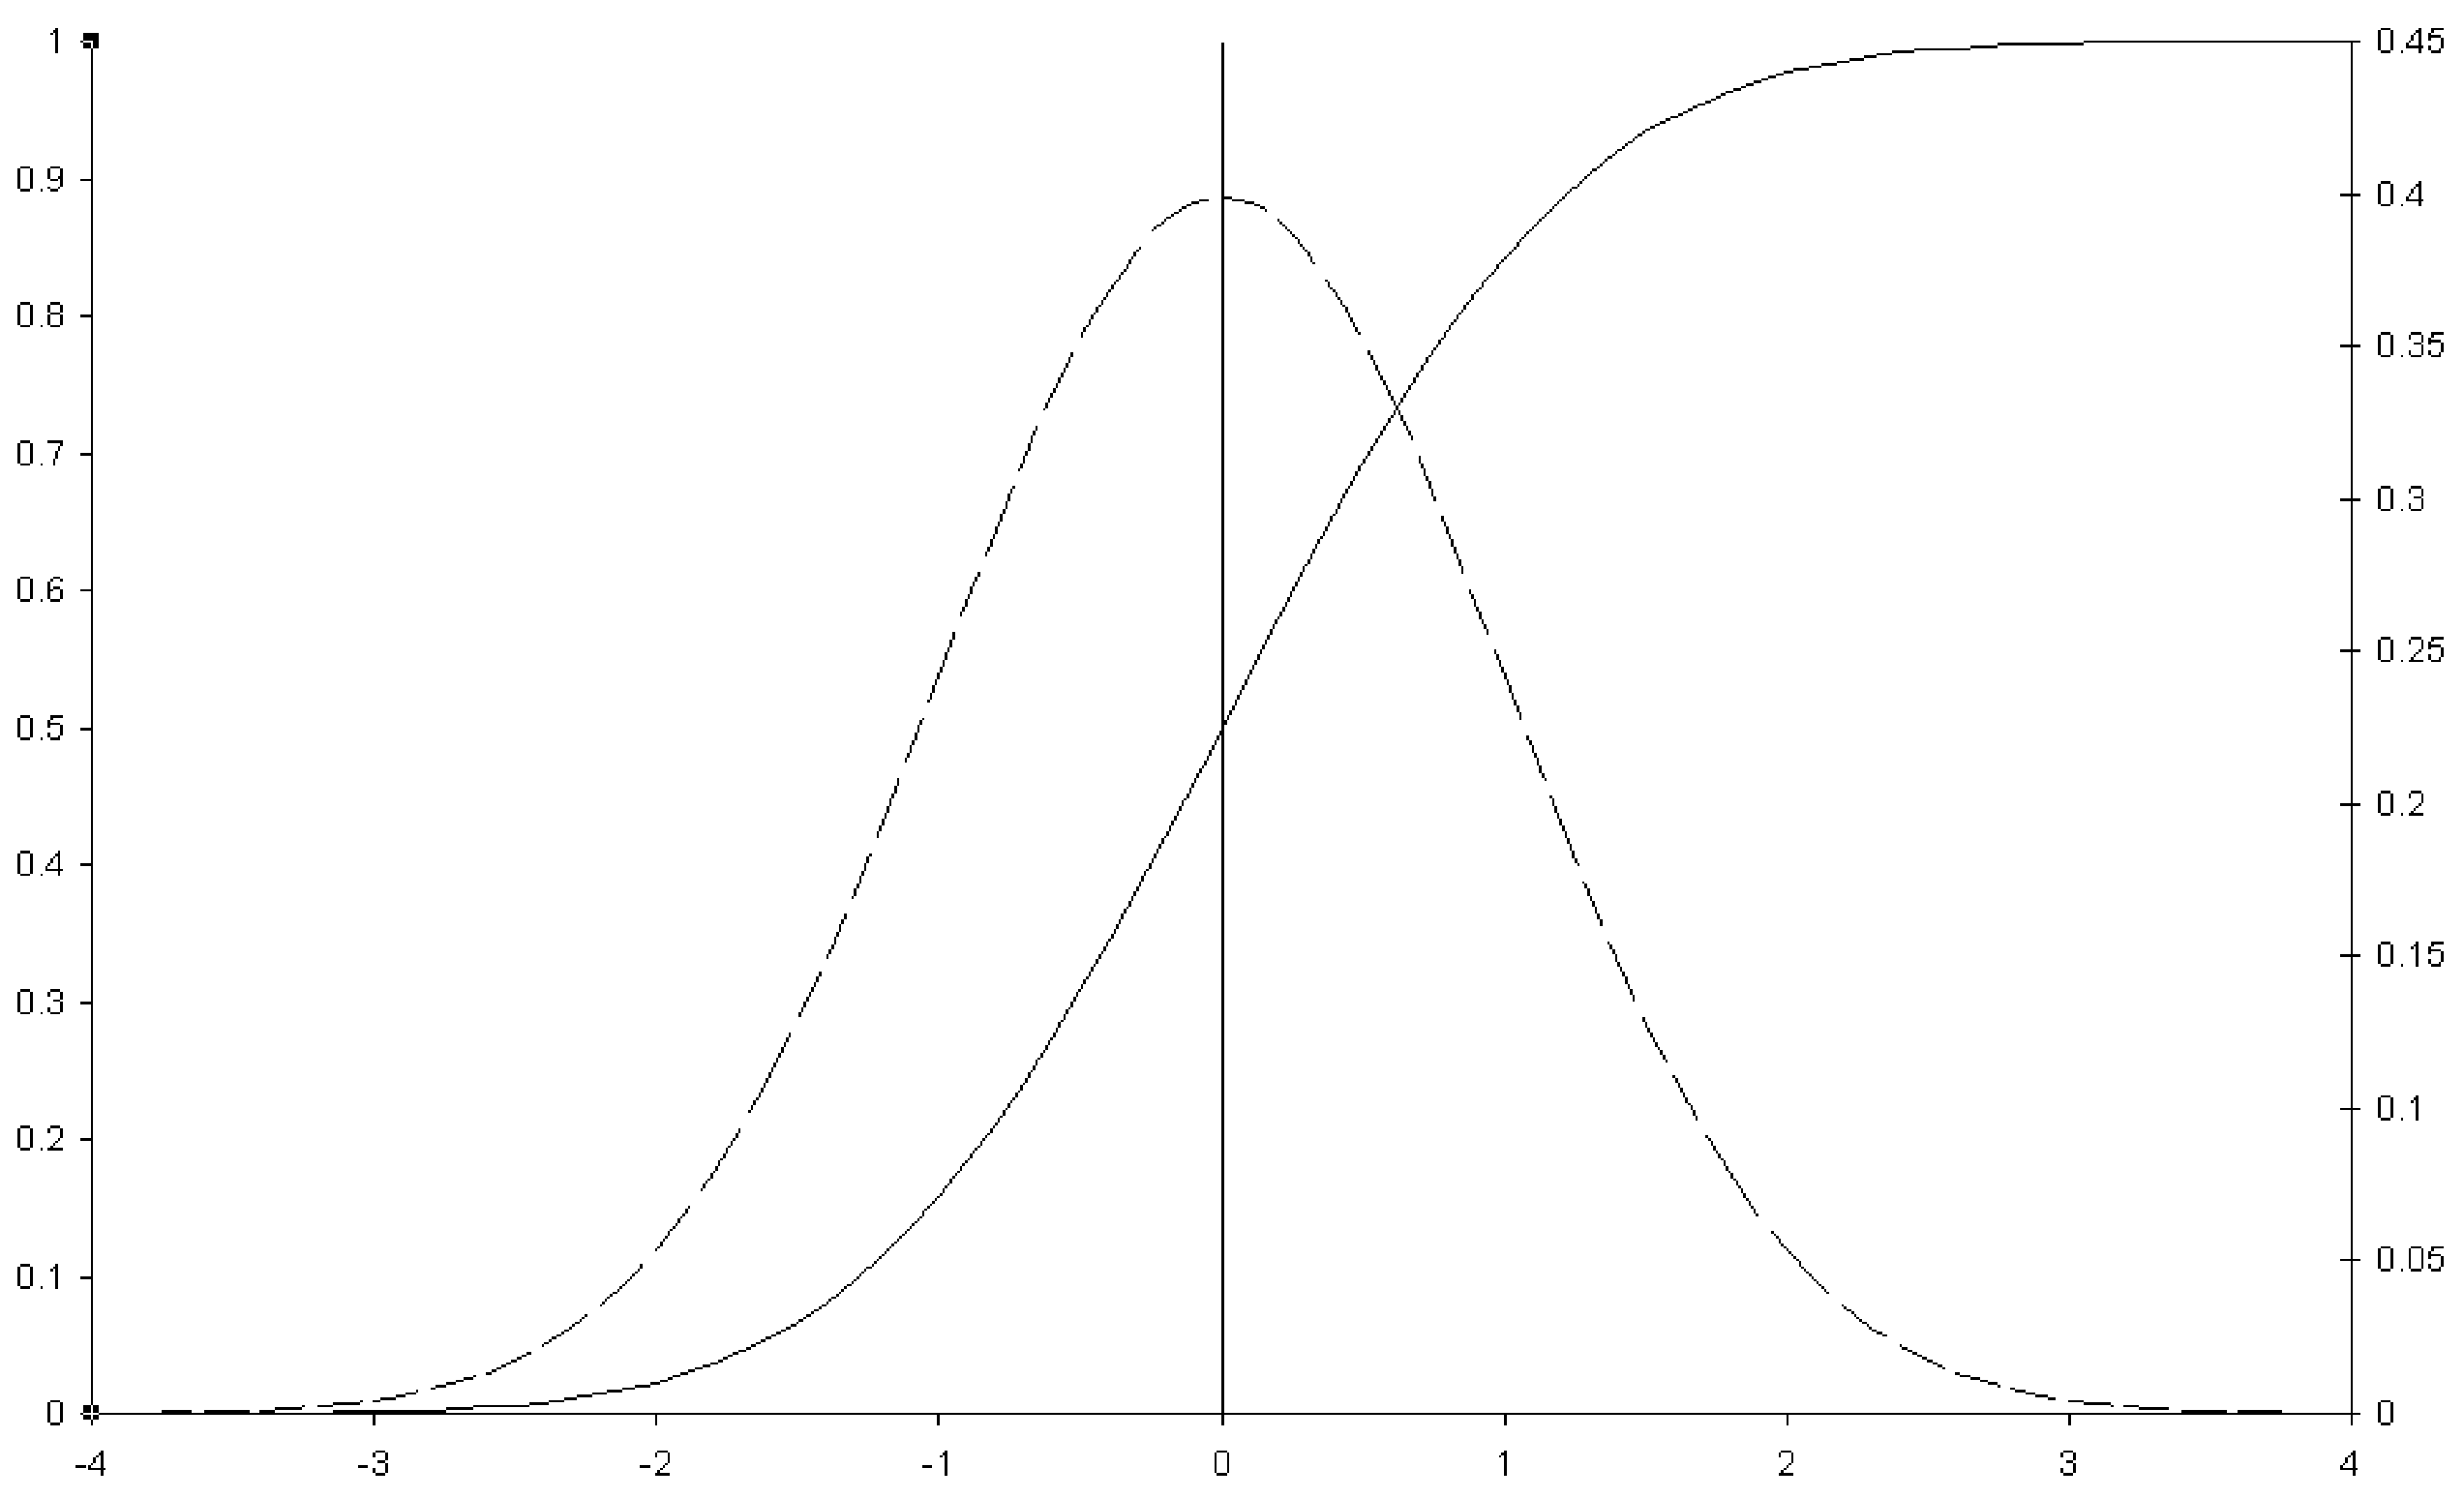
\includegraphics[width=8cm]{Figures/ErrorFunction}
\caption{The error function and the normal distribution}
\label{fig:errorFunction}
\end{figure}
The error function is the integral of the normal distribution. The
error function is used in statistics to evaluate the probability
of finding a measurement larger than a given value when the
measurements are distributed according to a normal distribution.
Figure \ref{sec:errorFunction} shows the familiar bell-shaped
curve of the probability density function of the normal
distribution (dotted line) together with the error function (solid
line).

In medical sciences one calls {\textsl centile} the value of the error
function expressed in percent. For example, obstetricians look
whether the weight at birth of the first born child is located
below the $10^{\mbox{th}}$ centile or above the $90^{\mbox{th}}$
centile to assess a risk factor for a second
pregnancy\footnote{\cf footnote \ref{ft:steer} on page
\pageref{ft:steer}}.

\subsection{Mathematical definitions}
\label{sec:errorFunctionDef} Because it is the integral of the
normal distribution, the error function, $\erf\left(x\right)$,
gives the probability of finding a value lower than $x$ when the
values are distributed according to a normal distribution with
mean 0 and standard deviation 1. The mean and the standard
deviation are explained in section \ref{sec:moments}. This
probability is expressed by the following integral\footnote{In
\cite{AbrSteg} and \cite{Press}, the error function is defined as:
$$\erf\left(x\right)={2 \over \sqrt{\pi}}\int_0^x e^{-{t^2 \over 2
}}dt$$.}:
\begin{equation}
\erf\left(x\right)={1 \over \sqrt{2\pi}}\int_{-\infty}^x e^{-{t^2
\over 2 }}dt
\end{equation}
The result of the error function lies between 0 and 1.

One could carry out the integral numerically, but there exists
several good approximations. The following formula is taken from
\cite{AbrSteg}.
\begin{mainEquation}
\label{eq:erf} \erf\left(x\right)={1 \over \sqrt{2\pi}}e^{-{x^2
\over 2 }}\sum_{i=1}^5 a_i r\left(x\right)^i\mbox{\quad for $x\ge
0$}.
\end{mainEquation}
where
\begin{equation}
\label{eq:erfpol}r\left(x\right)={1 \over {1-0.2316419x}}.
\end{equation}
and
\begin{equation}
\label{eq:erfconst}\left\{ \begin{array}{lr}a_1 =&0.31938153 \\
a_2 =&-0.356563782
\\a_3 =&1.7814779372 \\ a_4 =&-1.821255978 \\ a_5 =&1.330274429
\end{array}\right.
\end{equation}
The error on this formula is better than $7.5\times10^{-8}$ for
negative $x$.
To compute the value for positive values, one uses the fact that:
\begin{mainEquation}
\label{eq:erfneg} \erf\left(x\right)=1-\erf\left(-x\right).
\end{mainEquation}
When dealing with a general Gaussian distribution with average
$\mu$ and standard deviation $\sigma$ it is convenient to define a
generalized error function as:
\begin{equation}
\erf\left(x;\mu,\sigma\right)={1 \over
\sqrt{2\pi\sigma^2}}\int_{-\infty}^x e^{-{{\left(x-\mu\right)}^2
\over 2 \sigma^2}}dt.
\end{equation}
A simple change of variable in the integral shows that the
generalized error function can be obtained from the error function
as:
\begin{mainEquation}
\erf\left(x;\mu,\sigma\right)=\erf\left({x-\mu\over\sigma}\right).
\end{mainEquation}
Thus, one can compute the probability of finding a measurement $x$
within the interval $\left[\mu - t \cdot \sigma,\mu + t \cdot
\sigma\right] $ when the measurements are distributed according to
a Gaussian distribution with average $\mu$ and standard deviation
$\sigma$:
\begin{equation}
\label{eq:normaccept}
\prob\left({\left|x-\mu\right|\over\sigma}\le t\right)=2 \cdot
\erf\left(t\right)-1.\mbox{\quad for $t\ge 0$}.
\end{equation}

\rubrique{Example}
\def\w{2.85}\def\av{3.39}\def\st{0.44}
 Now we can give the answer to the problem of deciding
whether a pregnant woman needs special attention during her second
pregnancy. Let the weight at birth of her first child be $\w\kg$.
and let the duration of her first pregnancy be 39 weeks. In this
case measurements over a representative sample of all births
yielding healthy babies have an average of $\av\kg$ and a standard
deviation of $\st\kg$\footnote{\label{ft:steer}This is the
practice at the department of obstetrics and gynecology of the
Chelsea $\&$ Westminster Hospital of London. The numbers are
reproduced with permission of Prof. P.J. Steer.}. The probability
of having a weight of birth smaller than that of the woman's first
child is:
\begin{eqnarray*}
\prob\left(\mathop{\textrm Weight}\le \w\kg \right) & = &
\erf\left({\w-\av\over\st}\right),\\ & = & 11.2\%.
\end{eqnarray*}
According to current practice, this second pregnancy does not
require special attention.

\subsection{Error function --- Smalltalk implementation}
\label{sec:sterrorfunction} \marginpar{Figure \ref{fig:functions}
with the box {\textbf ErfApproximation} grayed.} The error function is
implemented as a single method for the class Number. Thus,
computing the centile of our preceding example is simply coded as:
\begin{displaycode}{Smalltalk}
| weight average stDev centile |
weight := 2.85.
average := 3.39.
stDev := 0.44.
centile := ((weight - average) / stDev) erf * 100.
\end{displaycode}
If you want to compute the probability for a measurement to lay
within 3 standard deviations from its mean, you need to evaluate
the following expression using equation \ref{eq:normaccept}:
\begin{displaycode}{Smalltalk}
3 errorFunction * 2 - 1.
\end{displaycode}
If one needs to use the error function as a function, one must use
it inside a block closure. In this case one defines a function
object as follows:
\begin{displaycode}{Smalltalk}
| errorFunction |
errorFunction := [:x | x errorFunction].
\end{displaycode}

Listing \ref{lst:errorFunction} shows the Smalltalk implementation
of the error function.

In Smalltalk we are allowed to extend existing classes. Thus, the
public method to evaluate the error function is implemented as a
method of the base class \code{Number}. This method uses the class,
\code{PMErfApproximation}, used to store the constants of equation
\ref{eq:erfconst} and evaluate the formula of equations
\ref{eq:erf} and \ref{eq:erfpol}. In our case, there is no need to
create a separate instance of the class \code{PMErfApproximation}
at each time since all instances would actually be exactly
identical. Thus, the class \code{PMErfApproximation} is a
singleton class. A singleton class is a class, which can only
create a single instance \cite{GoF}. Once the first instance is
created, it is kept in a class instance variable. Any subsequent
attempt to create an additional instance will return a pointer to
the class instance variable holding the first created instance.

One could have implemented all of these methods as class methods
to avoid the singleton class. In Smalltalk, however, one tends to
reserve class method for behavior needed by the structural
definition of the class. So, the use of a singleton class is
preferable. A more detailed discussion of this topic can be found
in \cite{StDesPat}.

\begin{listing}[label=lst:errorFunction]{Smalltalk}
{Smalltalk implementation of the Error function}
Number >> errorFunction
    ^PMErfApproximation new value: self
\end{listing}

\begin{displaycode}{Smalltalk}
Object subclass: #PMErfApproximation
   instanceVariableNames: 'constant series norm'
   classVariableNames: 'UniqueInstance'
   package: 'Math-Core-Distribution'
\end{displaycode}

\begin{displaycode}{Smalltalk}
PMErfApproximation class >> new
    UniqueInstance isNil
        ifTrue: [UniqueInstance := super new initialize].
    ^UniqueInstance
\end{displaycode}

\begin{displaycode}{Smalltalk}
PMErfApproximation >> initialize
    constant := 0.2316419.
    norm := 1 / (Float pi * 2) sqrt.
    series := PMPolynomial coefficients: #( 0.31938153 -0.356563782 
                               1.781477937 -1.821255978 1.330274429). 
\end{displaycode}

\begin{displaycode}{Smalltalk}
PMErfApproximation >> normal: aNumber
   "Computes the value of the Normal distribution for aNumber"

   ^ [ (aNumber squared * -0.5) exp * norm ]
     on: Error
     do: [ :signal | signal return: 0 ]
\end{displaycode}

\begin{displaycode}{Smalltalk}
PMErfApproximation >> value: aNumber
    | t |
    aNumber = 0
        ifTrue: [ ^0.5].
    aNumber > 0
        ifTrue: [ ^1- ( self value: aNumber negated)].
    aNumber < -20
        ifTrue: [ ^0].
    t := 1 / (1 - (constant * aNumber)).
    ^(series value: t) * t * (self normal: aNumber)
\end{displaycode}

\section{Gamma function}
The gamma function is used in many mathematical functions. In this
book, the gamma function is needed to compute the normalization
factor of several probability density functions (\cf sections
\ref{sec:gammadist} and \ref{sec:chitest}). It is also needed to
compute the beta function (\cf section \ref{sec:betafunc}).

\subsection{Mathematical definitions}
\label{sec:gammafunc} The Gamma function is defined by the
following integral, called Euler's integral\footnote{Leonard Euler
to be precise as the Euler family produced many mathematicians.}:
\begin{equation}
\label{eq:gammafunc} \Gamma\left(x\right)=\int_0^\infty t^x
e^{-t}dt
\end{equation}
From equation \ref{eq:gammafunc} a recurrence formula can be
derived:
\begin{equation}
\label{eq:gammarec} \Gamma\left(x+1\right)=x \cdot
\Gamma\left(x\right)
\end{equation}
The value of the Gamma function can be computed for special values
of $x$:
\begin{equation}
\label{eq:gammaval}\left\{
\begin{array}{lr}\Gamma\left(1\right)=1\\\Gamma\left(2\right)=1
\end{array}\right.
\end{equation}
From \ref{eq:gammarec} and \ref{eq:gammaval}, the well-known
relation between the value of the Gamma function for positive
integers and the factorial can be derived:
\begin{equation}
\label{eq:gammafact} \Gamma\left(n\right)=\left(n-1\right)!
\mbox{\quad for $n>0$}.
\end{equation}
The most precise approximation for the Gamma function is given by
a formula discovered by Lanczos \cite{Press}:
\begin{mainEquation}
\label{eq:lanczos} \Gamma\left(x\right)\approx e^{\left(x+{5\over
2}\right)}\left(x+{5\over 2}\right){\sqrt{2\pi}\over x
}\left(c_0+\sum_{n=1}^6{c_n \over x + n}+\epsilon\right)
\end{mainEquation}
where
\begin{equation}
\label{eq:lanczosconst}\left\{ \begin{array}{lrl}c_0
=&1.000000000190015
\\c_1 =&76.18009172947146 \\ c_2 =&-86.50532032941677
\\c_3 =&24.01409824083091 \\ c_4 =&-1.231739572450155
\\ c_5 =&1.208650973866179&\cdot 10^{-3} \\ c_6 =&-5.395239384953&\cdot 10^{-6}
\end{array}\right.
\end{equation}
This formula approximates $\Gamma\left(x\right)$ for $x>1$ with
$\epsilon<2\cdot 10^{-10}$ . Actually, this remarkable formula can
be used to compute the gamma function of any complex number $z$
with $\Re\left(z\right)>1$ to the quoted precision. Combining
Lanczos' formula with the recurrence formula \ref{eq:gammarec} is
sufficient to compute values of the Gamma function for all
positive numbers.

For example, $\Gamma\left({3\over 2}\right)={\sqrt{\pi}\over 2}=
0.886226925452758$ whereas Lanczos formula yields the value
$0.886226925452754$, that is, an absolute error of $4\cdot
10^{-15} $. The corresponding relative precision is almost equal
to the floating-point precision of the machine on which this
computation was made.

Although this is seldom used, the value of the Gamma function for
negative non-integer numbers can be computed using the reflection
formula hereafter:
\begin{equation}
\label{eq:gammaneg} \Gamma\left(x\right)={\pi\over
\Gamma\left(1-x\right) \sin\pi x}
\end{equation}

In summary, the algorithm to compute the Gamma function for any
argument goes as follows:
\begin{enumerate}
  \item If $x$ is a non-positive integer ($x\le0$), raise an exception.
  \item If $x$ is smaller than or equal to 1 ($x<1$), use the recurrence formula \ref{eq:gammarec}.
  \item If $x$ is negative ($x<0$, but non integer), use the reflection
formula \ref{eq:gammaneg}.
  \item Otherwise use Lanczos' formula \ref{eq:lanczos}.
\end{enumerate}

One can see from the leading term of Lanczos' formula that the
gamma function raises faster than an exponential. Thus, evaluating
the gamma function for numbers larger than a few hundreds will
exceed the capacity of the floating number representation on most
machines. For example, the maximum exponent of a double precision
IEEE floating-point number is 1024. Evaluating directly the
following expression:
\begin{equation}
\label{eq:gammaovfl}
  {\Gamma\left(460.5\right)\over\Gamma\left(456.3\right)}
\end{equation}
will fail since $\Gamma\left(460.5\right)$ is larger than
$10^{1024}$. Thus, its evaluation yields a floating-point overflow
exception. It is therefore recommended to use the logarithm of the
gamma function whenever it is used in quotients involving large
numbers. The expression of equation \ref{eq:gammaovfl} is then
evaluated as:
\begin{equation}
  \exp\left[\ln\Gamma\left(460.5\right)-\ln\Gamma\left(456.3\right)\right]
\end{equation}
which yield the result $1.497\cdot 10^{11}$. That result fits
comfortably within the floating-point representation.

For similar reasons the leading factors of Lanczos formula are
evaluated using logarithms in both implementations.

\subsection{Gamma function --- Smalltalk implementation}
\marginpar{Figure \ref{fig:functions} with the box {\textbf
LanczosFormula} grayed.} Like the error function, the gamma
function is implemented as a single method of the class {\texttt
Number}. Thus, computing the gamma function of 2.5 is simply coded
as:
\begin{listing}{Smalltalk}
2.5 gamma
\end{listing}
To obtain the logarithm of the gamma function, you need to
evaluate the following expression:
\begin{listing}{Smalltalk}
2.5 logGamma
\end{listing}

Listing \ref{ls:gammafunc} shows the Smalltalk implementation of the gamma
function.

Here, the gamma function is implemented with two methods: one for
the class {\texttt Integer} and one for the class {\texttt Float}.
Otherwise, the scheme to define the gamma function is similar to
that of the error function. Please refer to section
\ref{sec:sterrorfunction} for detailed explanations.

Since the method factorial is already defined for integers in the
base classes, the gamma function has been defined using equation
\ref{eq:gammafact} for integers. An error is generated if one
attempts to compute the gamma function for non-positive integers.
The class {\texttt Number} delegates the computation of Lanczos'
formula to a singleton class. This is used by the non-integer
subclasses of {\texttt Number}: {\texttt Float} and {\texttt Fraction}.

The execution time to compute the gamma function for floating
argument given in Table \ref{tb:speed} in section \ref{sec:speed}.
\begin{listing}[label=ls:gammafunc]{Smalltalk}
{Smalltalk implementation of the gamma function}
$$\halign{ #\hfil&\quad#\hfil\cr {\sl Class}& {\Large\bf Integer}\cr
{\sl Subclass of }&{\tt Number}\cr\noalign{\vskip 1ex}
}$$


Instance methods
{\parskip 1ex\par\noindent}
{\bf gamma}
\begin{verbatim}
    self > 0
        ifFalse: [ ^self error: 'Attempt to compute the Gamma 
        function of a non-positive integer'].
    ^( self - 1) factorial
\end{verbatim}


$$\halign{ #\hfil&\quad#\hfil\cr {\sl Class}& {\Large\bf Number}\cr
{\sl Subclass of }&{\tt Magnitude}\cr\noalign{\vskip 1ex}
}$$


Instance methods
{\parskip 1ex\par\noindent}
{\bf gamma}
\begin{verbatim}
    ^self > 1
        ifTrue: [ ^DhbLanczosFormula new gamma: self]
        ifFalse:[ self < 0
                     ifTrue: [ Float pi / ( ( Float pi * self) sin * ( 1 - self) gamma)]
                     ifFalse:[ ( DhbLanczosFormula new gamma: (self + 1)) / self]
                    ]
\end{verbatim}
{\bf logGamma}
\begin{verbatim}
    ^self > 1
        ifTrue: [ DhbLanczosFormula new logGamma: self]
        ifFalse: [ self > 0
                      ifTrue: [ ( DhbLanczosFormula new logGamma: (self + 1)) - self ln ]
                      ifFalse: [ ^self error: 'Argument for the log gamma function
                         must be positive']
                    ]
\end{verbatim}


$$\halign{ #\hfil&\quad#\hfil\cr {\sl Class}& {\Large\bf DhbLanczosFormula}\cr
{\sl Subclass of }&{\tt Object}\cr\noalign{\vskip 1ex}

{\sl Instance variable names:}&\parbox[t]{4 in}{\tt  coefficients sqrt2Pi }\cr\noalign{\vskip 1ex}
{\sl Class variable names:}&\parbox[t]{4 in}{\tt  UniqueInstance }\cr\noalign{\vskip 1ex}}$$


Class methods
{\parskip 1ex\par\noindent}
{\bf new}
\begin{verbatim}
    UniqueInstance isNil
        ifTrue: [ UniqueInstance := super new initialize ].
    ^ UniqueInstance
\end{verbatim}

Instance methods
{\parskip 1ex\par\noindent}
{\bf gamma:} {\tt aNumber}
\begin{verbatim}
    ^ (self leadingFactor: aNumber) exp * (self series: aNumber) 
        * sqrt2Pi / aNumber
\end{verbatim}
{\bf initialize}
\begin{verbatim}
    sqrt2Pi := ( Float pi * 2) sqrt.
    coefficients := #( 76.18009172947146 -86.50532032941677 
           24.01409824083091 -1.231739572450155 0.1208650973866179e-2 
           -0.5395239384953e-5).
    ^ self
\end{verbatim}
{\bf leadingFactor:} {\tt aNumber}
\begin{verbatim}
    | temp |
    temp := aNumber + 5.5.
    ^ (temp ln * ( aNumber + 0.5) - temp)
\end{verbatim}
{\bf logGamma:} {\tt aNumber}
\begin{verbatim}
    ^ (self leadingFactor: aNumber) + ((self series: aNumber) 
    * sqrt2Pi / aNumber) ln
\end{verbatim}
{\bf series:} {\tt aNumber}
\begin{verbatim}
    | term |
    term := aNumber.
    ^coefficients inject: 1.000000000190015
                        into: [ :sum :each | term := term + 1. each / term + sum ]
\end{verbatim}


\end{listing}

\section{Beta function}
\label{sec:betafunc} The beta function is directly related to the
gamma function. In this book, the beta function is needed to
compute the normalization factor of several probability density
functions (\cf sections \ref{sec:Ftest}, \ref{sec:ttest} and
\ref{sec:betadist}).
\subsection{Mathematical definitions}
The beta function is defined by the following integral:
\begin{equation}
\label{eq:betaint} B\left(x,y\right)=\int_0^1
t^{x-1}\left(1-t\right)^{y-1}dt
\end{equation}
The beta function is related to the gamma function with the
following relation:
\begin{equation}
B\left(x,y\right)={\Gamma\left(x\right)\Gamma\left(y\right)\over\Gamma\left(x+y\right)}
\end{equation}
Thus, computation of the beta function is directly obtained from
the gamma function. As evaluating the gamma function might
overflow the floating-point exponent (\cf discussion at the end of
section \ref{sec:gammafunc}), it is best to evaluate the above
formula using the logarithm of the gamma function.

\subsection{Beta function --- Smalltalk implementation}
\marginpar{Figure \ref{fig:functions} with the box {\textbf
LanczosFormula} grayed.} Like the error and gamma functions, the
gamma function is implemented as a single method of the class {\texttt
Number}. Thus, computing the beta function of 2.5 and 5.5 is
simply coded as:
\begin{listing}{Smalltalk}
2.5 beta: 5.5
\end{listing}

Computing the logarithm of the beta function of
2.5 and 5.5 is simply coded as:
\begin{listing}{Smalltalk}
2.5 logBeta: 5.5
\end{listing}
Listing \ref{ls:betafunc} shows the
implementation of the beta function in Smalltalk.

\begin{listing}[label=ls:betafun]{Smalltalk}
{Smalltalk implementation of the beta function}
$$\halign{ #\hfil&\quad#\hfil\cr {\sl Class}& {\Large\bf Number}\cr
{\sl Subclass of }&{\tt Magnitude}\cr\noalign{\vskip 1ex}
}$$


Instance methods
{\parskip 1ex\par\noindent}
{\bf beta:} {\tt aNumber}
\begin{verbatim}
    ^ (self logBeta: aNumber) exp
\end{verbatim}
{\bf logBeta:} {\tt aNumber}
\begin{verbatim}
    ^ self logGamma + aNumber logGamma - ( self + aNumber) logGamma
\end{verbatim}


\end{listing}

%\ifx\wholebook\relax\else\end{document}\fi

%\ifx\wholebook\relax\else
%\documentclass[twoside]{book}
%\usepackage[active]{srcltx}
%\usepackage[LY1]{fontenc}
%\usepackage{url}
\makeatletter
\def\url@leostyle{%
  \@ifundefined{selectfont}{\def\UrlFont{\sf}}{\def\UrlFont{\sffamily}}}
\makeatother
% Now actually use the newly defined style.
\urlstyle{leo}

\usepackage{graphicx}
\def\etc{{\textit{etc}}}
\def\eg{{\textit{e.g.}}}
\def\ie{{\textit{i.e.}}}
\def\cf{{\textit{c.f.}}\ }
\def\erf{\mathop{\textrm{erf}}}
\def\sign{\mathop{\textrm{sign}}}
\def\prob{\mathop{\textrm{Prob}}}
\def\var{\mathop{\textrm{var}}}
\def\mod{\mathop{\textrm{mod}}}
\def\cor{\mathop{\textrm{cor}}}
\def\cov{\mathop{\textrm{cov}}}
\def\cl{\mathop{\textrm{CL}}}
\def\kg{\mathop{\textrm{Kg}}}
\def\patstyle#1{{\textsc #1}}
\def\th{^{\mathop{\textrm{th}}}}
%\def\st#1{^{\mathop{\rm #1}}}
\def\note#1{\begin{quote}{\textbf{Note:}} #1\end{quote}}
\def\braket#1{\left\langle #1\right\rangle}
\def\order#1{\let\o=#1$\mathcal{O}$\ifx\o 1$\left(n\right)$\else$\left(n^{#1}\right)$\fi}
%\newtheorem{privListing}{Listing}[chapter]
%\newenvironment{listing}{\vskip 3ex\hrule\vskip 1ex\begin{privListing}}{\end{privListing}\hrule\vskip 1ex}
\newtheorem{privExample}{Code example}[chapter]
\newenvironment{codeExample}{\begin{privExample}\begin{quote}\tt}{\end{quote}\end{privExample}}
\def\relboxl#1#2{\hbox to #1\hsize{#2\hfil}}
\def\relboxc#1#2{\hbox to #1\hsize{\hfil #2\hfil}}
\def\relboxr#1#2{\hbox to #1\hsize{\hfil #2}}
\def\transpose#1{\textbf{#1}^{\mathop\textrm{T}}}
\def\inverse#1{\textbf{#1}^{-1}}
%\def\tm{$^{\mathop{\rm TM}}$}
\def\tm{ }
\newenvironment{mainEquation}{\marginpar[\vspace{3 ex} Main
equation$\Rightarrow$]{\vspace{3 ex}$\Leftarrow$Main
equation}\begin{equation}}{\end{equation}}
\def\rubrique#1{\paragraph{#1}\hfil\par\noindent}

%\begin{document}
%\fi

\chapter{Interpolation}
\label{ch:interpolation}
\begin{flushright}
{\textsl On ne peut pr\'evoir les choses qu'apr\`es qu'elles sont
arriv\'ees.}\footnote{One can predict things only after they have
occurred.}\\ Eug\`ene Ionesco
\end{flushright}
\vspace{1 ex} Interpolation is a technique allowing the estimation
of a function over the range covered by a set of points at which
the function's values are known. These points are called the {\textsl
sample} points. Interpolation is useful to compute a function
whose evaluation is highly time consuming: with interpolation it
suffices to compute the function's values for a small number of
well-chosen sample points. Then, evaluation of the function
between the sample points can be made with interpolation.

Interpolation can also be used to compute the value of the inverse
function, that is finding a value $x$ such that
$f\left(x\right)=c$ where $c$ is a given number, when the function
is known for a few sample points bracketing the sought value.
People often overlook this easy and direct computation of the
inverse function.

Interpolation is often used interchangeably with extrapolation.
This is not correct, however. Extrapolation is the task of
estimating a function outside of the range covered by the sample
points. If no model exists for the data extrapolation is just
gambling. Methods exposed in this chapter should not be used for
extrapolation.

Interpolation should not be mistaken with function (or curve)
fitting. In the case of interpolation the sample points purely
determine the interpolated function. Function fitting allows
constraining the fitted function independently from the sample
points. As a result fitted functions are more stable than
interpolated functions especially when the supplied values are
subject to fluctuations coming from rounding or measurement
errors. Fitting is discussed in chapter \ref{ch:estimation}.

\section{General remarks}
\label{sec:interpolgen} There are several methods of
interpolation. One difference is the type of function used. The
other is the particular algorithm used to determine the function.
For example, if the function is periodic, interpolation can be
obtained by computing a sufficient number of coefficients of the
Fourier series for that function.

In the absence of any information about the function, polynomial
interpolation gives fair results. The function should not have any
singularities over the range of interpolation. In addition there
should not be any pole in the vicinity of the complex plane near
the portion of the real axis corresponding to the range of
interpolation. If the function has singularities it is recommended
to use rational functions --- that is the quotient of two
polynomials --- instead \cite{Press}.

In this chapter we discuss 3 interpolation functions: Lagrange
interpolation polynomial, a diagonal rational function
(Bulirsch-Stoer interpolation) and cubic spline. Furhermore, we
show 3 different implementation of the Lagrange interpolation
polynomial: direct implementation of Lagrange's formula, Newton's
algorithm and Neville's algorithm.
\begin{figure}
\label{cls:interpolation}
\centering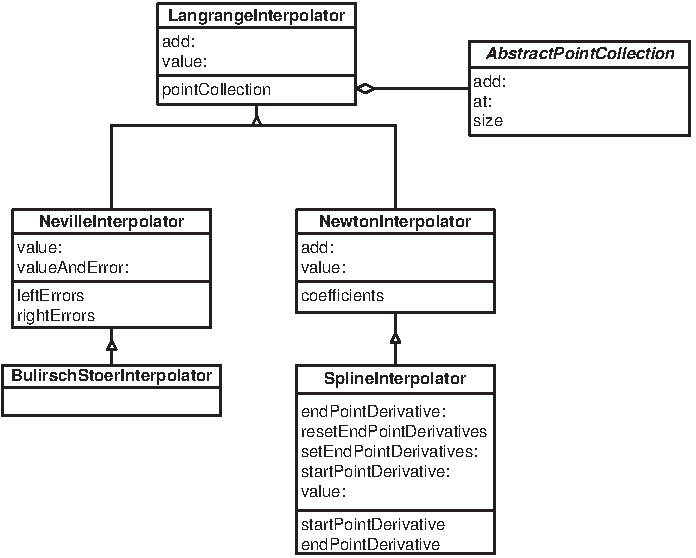
\includegraphics[width=11cm]{Figures/InterpolationClassDiagram}
\caption{Class diagram for the interpolation classes}
\end{figure}
Figure \ref{cls:interpolation} shows how the classes corresponding
to the different interpolation methods described in this chapter
are related to each other.

\rubrique{Definition} The {\textit Lagrange interpolation polynomial}
is the unique polynomial of minimum degree going through the
sample points. The degree of the polynomial is equal to the number
of supplied points minus one. A diagonal rational function is the
quotient of two polynomials where the degree of the polynomial in
the numerator is at most equal to that of the denominator. Cubic
spline uses piece-wise interpolation with polynomials but limits
the degree of each polynomial to 3 (hence the adjective cubic).

\rubrique{Examples} Before selecting an interpolation method the
user must investigate the validity of the interpolated function
over the range of its intended use. Let us illustrate this remark
with an example from high-energy physics, that, in addition, will
expose the limitation of the methods exposed in this chapter.

\begin{figure}
\label{fig:landauinterpol}
\centering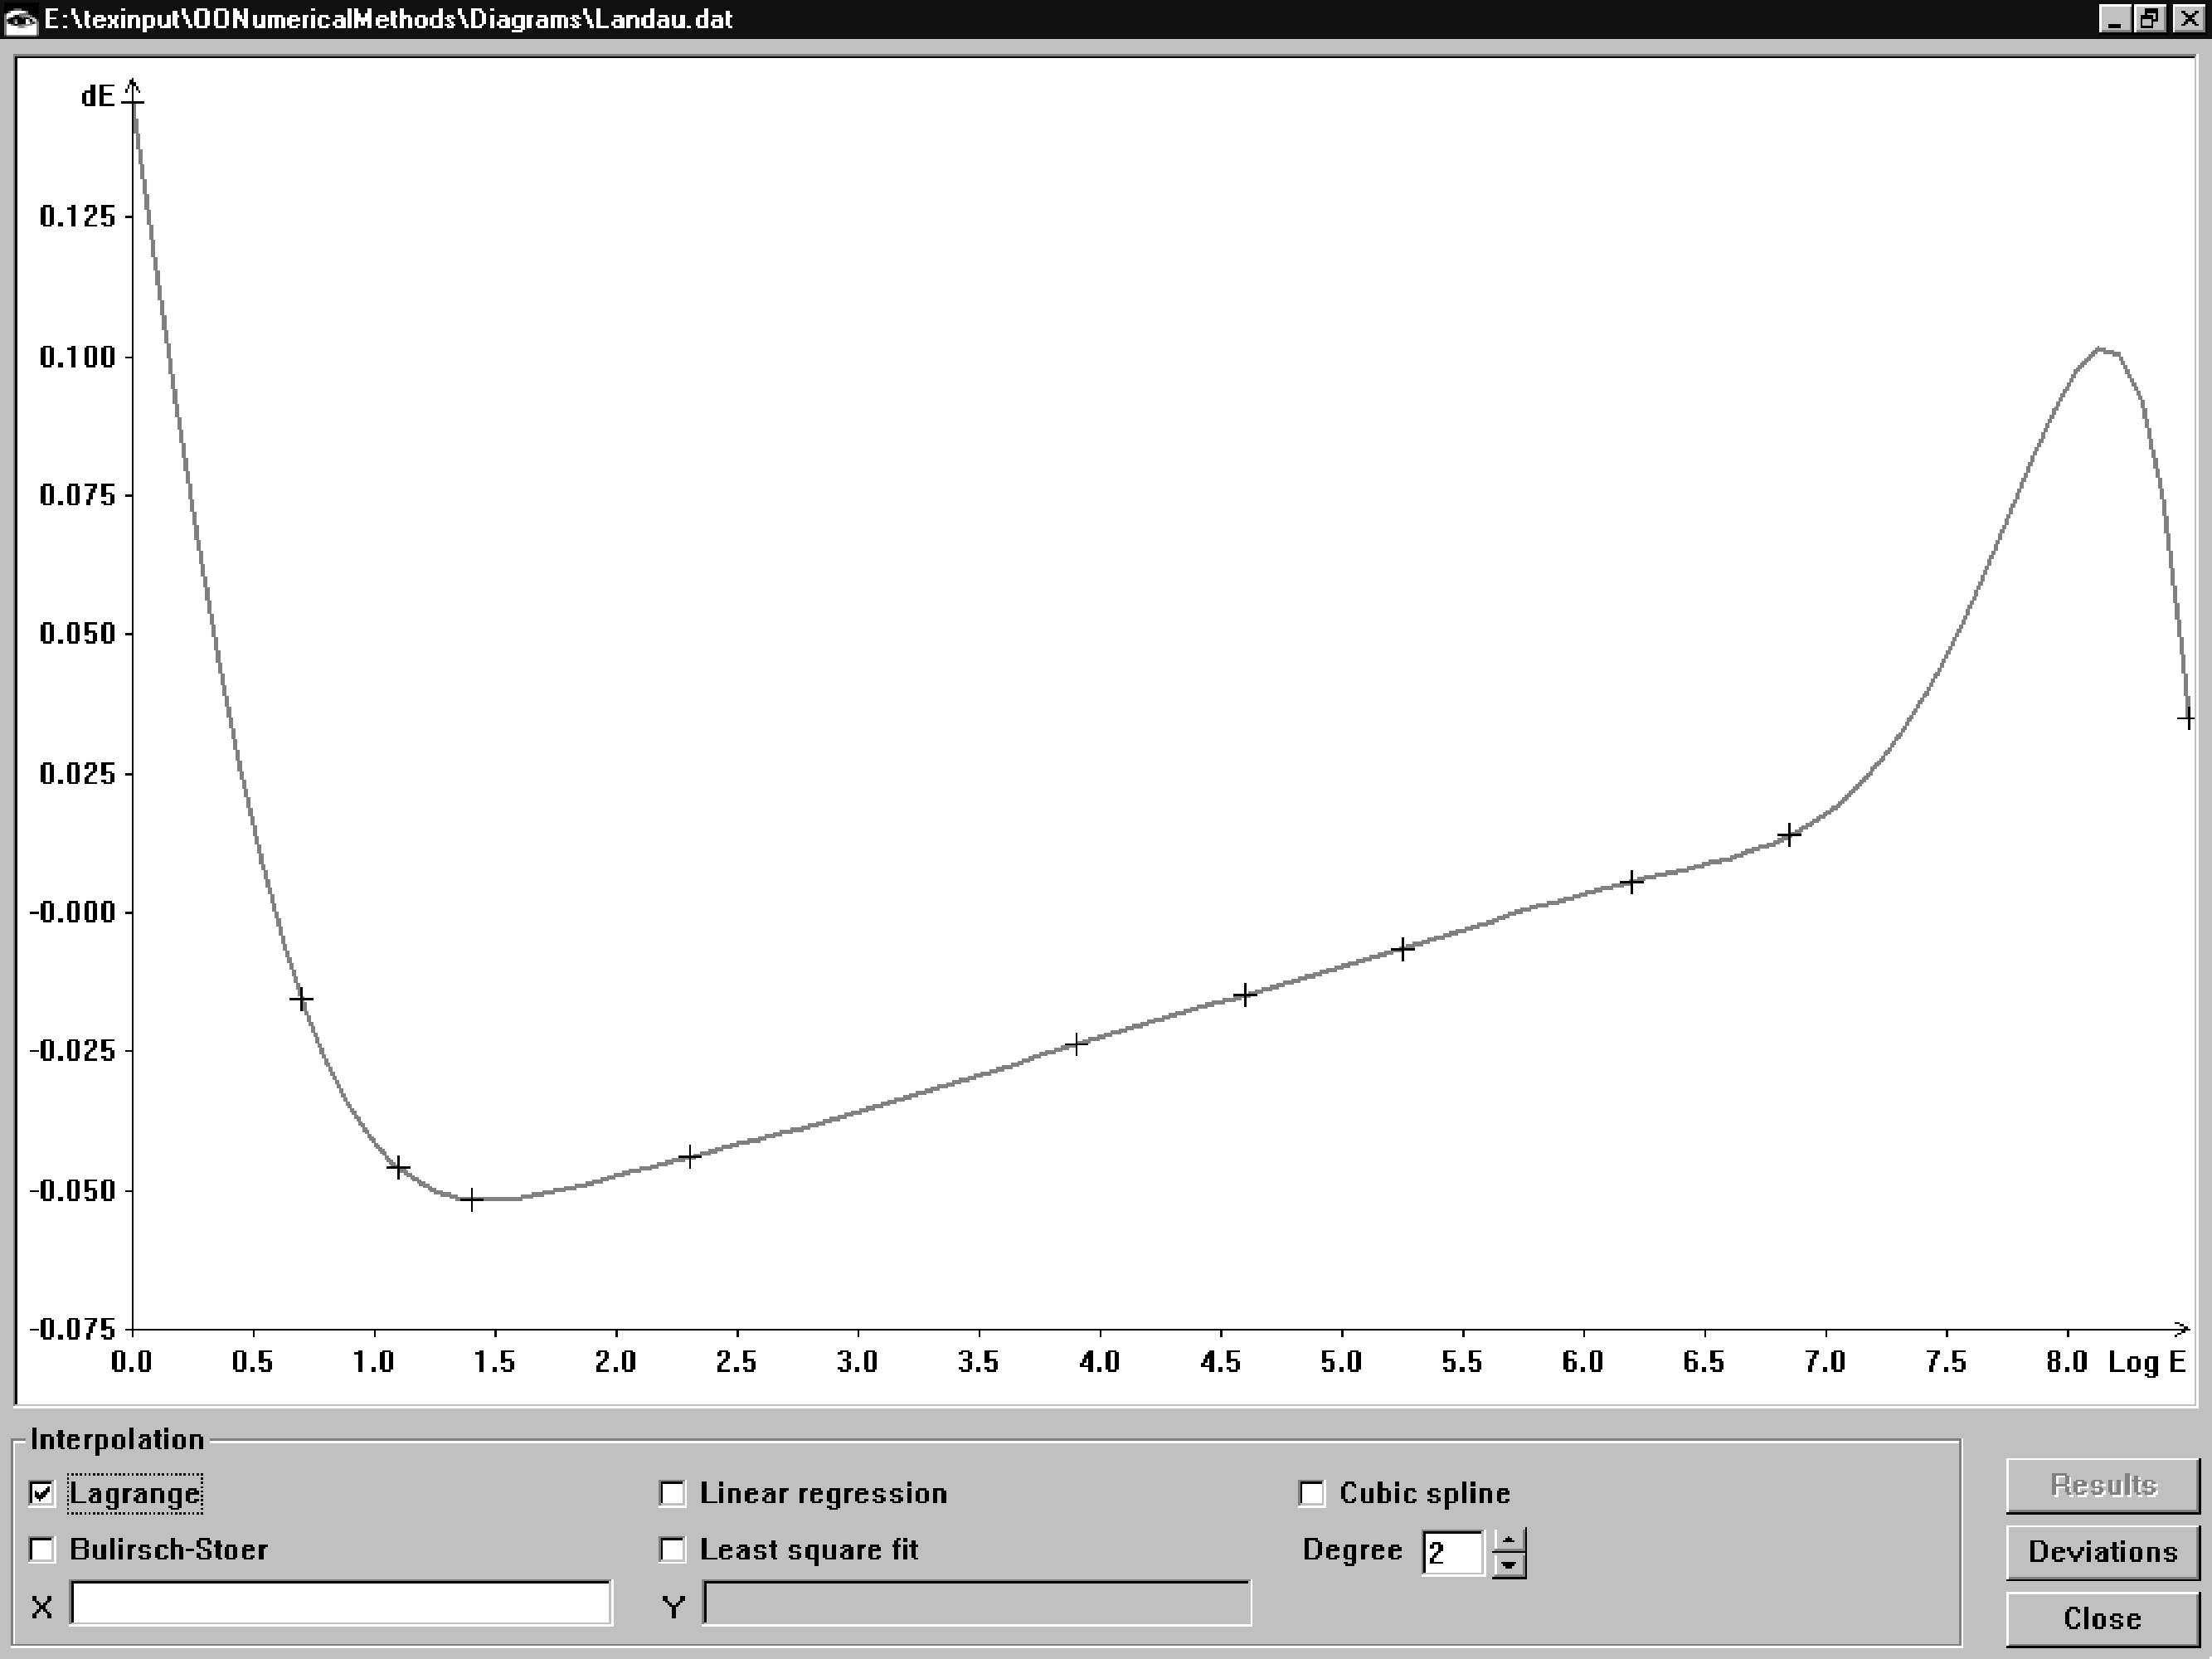
\includegraphics[width=12cm]{Figures/Lagrange}
\caption{Example of interpolation with the Lagrange interpolation
polynomial}
\end{figure}
Figure \ref{fig:landauinterpol} shows sample points --- indicated
by crosses --- representing correction to the energy measured
within a gamma ray detector made of several densely packed
crystals. The energy is plotted on a logarithmic scale. The
correction is caused by the absorption of energy in the wrapping
of each crystal. The sample points were computed using a
simulation program\footnote{This program - EGS written by Ralph
Nelson of the Stanford Linear Accelerator Center (SLAC) -
simulates the absorption of electromagnetic showers inside matter.
Besides being used in high-energy physics this program is also
used in radiology to dimension detectors of PET scanners and other
similar radiology equipment.}, each point requiring several hours
of computing time. Interpolation over these points was therefore
used to allow a quick computation of the correction at any energy.
This is the main point of this example: the determination of each
point was expensive in terms of computing time, but the function
represented by these points is continuous enough to be
interpolated. The simulation program yields results with good
precision so that the resulting data are not subjected to
fluctuation.

The gray thick line in figure \ref{fig:landauinterpol} shows the
Lagrange interpolation polynomial obtained from the sample points.
It readily shows limitations inherent to the use of interpolation
polynomials. The reader can see that for values above 6.5 ---
corresponding to an energy of 500 MeV --- the interpolated
function does not reproduce the curve corresponding to the sample
points. In fact, above 4.0 --- that is,  50 MeV on the scale of
figure \ref{fig:landauinterpol} --- the correction is expected to
be a linear function of the logarithm of the energy.

\begin{figure}
\label{fig:interpolex2}
\centering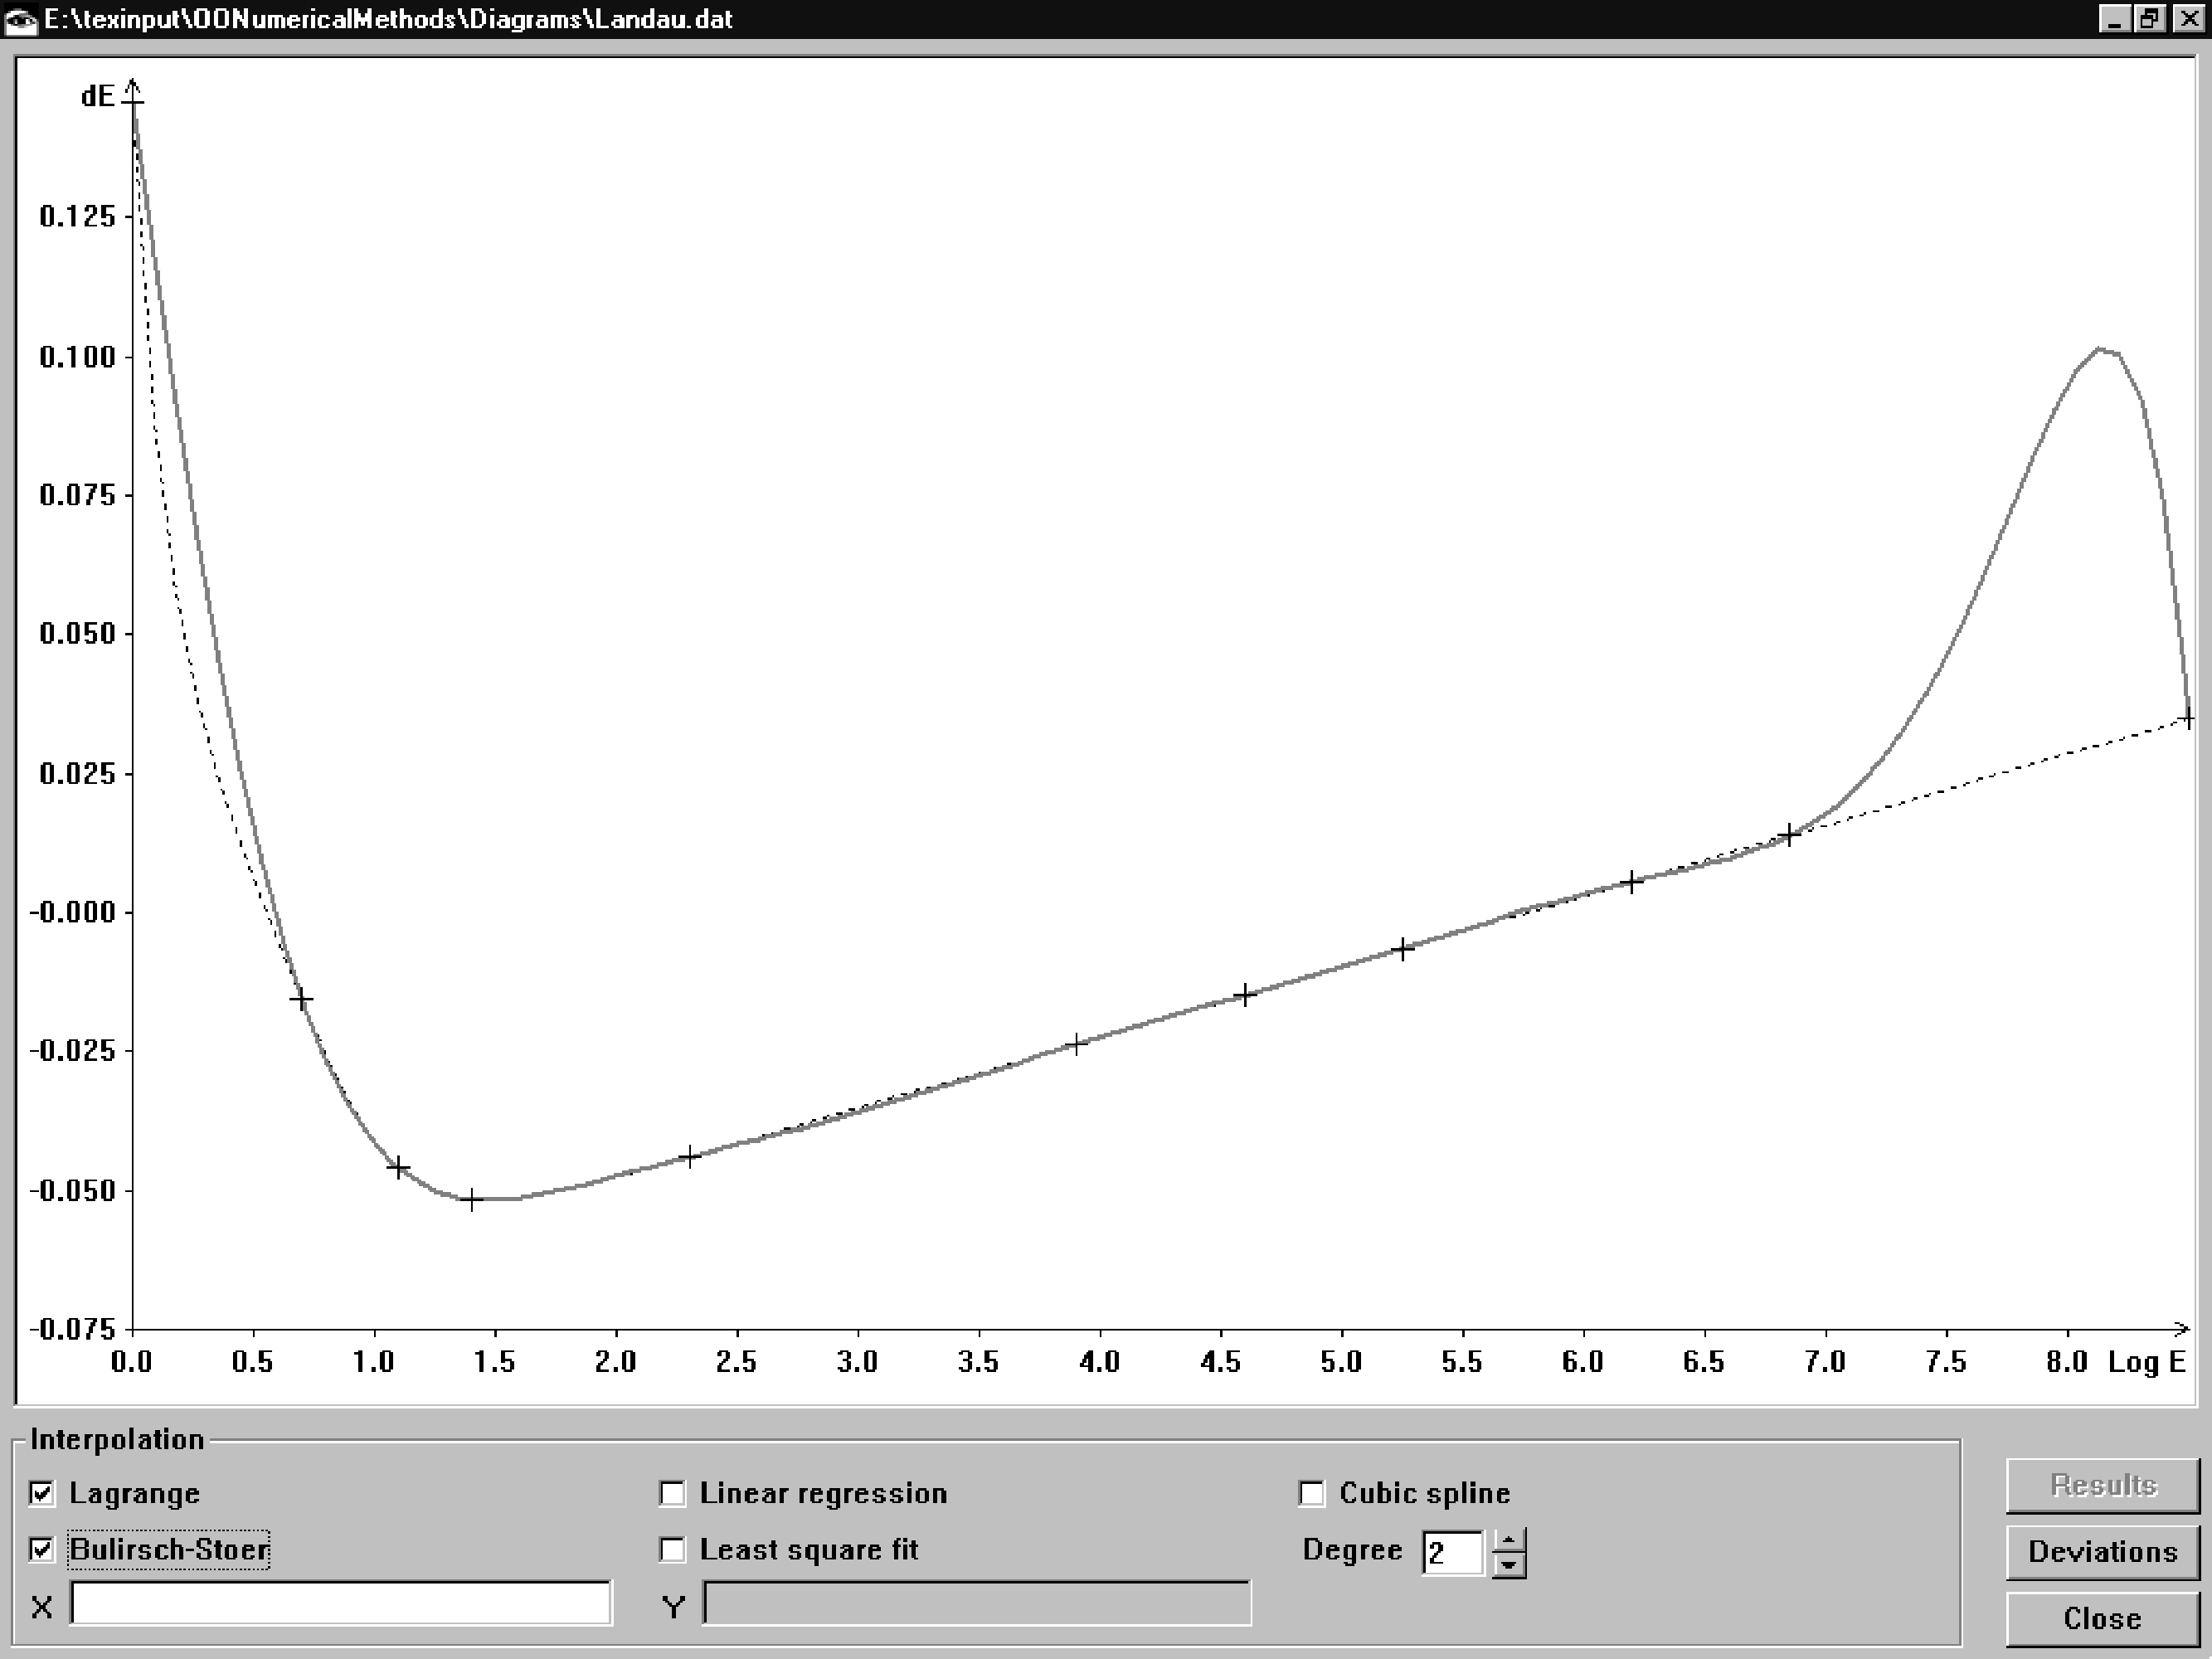
\includegraphics[width=12cm]{Figures/LagrangeVsRational}
\caption{Comparison between Lagrange interpolation and
interpolation with a rational function}
\end{figure}
Figure \ref{fig:interpolex2} shows a comparison between the
Lagrange interpolation polynomial (gray thick line) and
interpolation with a rational function (black dotted line) using
the same sample points as in figure \ref{fig:landauinterpol}. The
reader can see that, in the high-energy region (above 4 on the
scale of figure \ref{fig:interpolex2}) the rational function does
a better job than the Lagrange polynomial. Between the first two
points, however, the rational function fails to reproduce the
expected behavior.

\begin{figure}
\label{fig:interpolex3}
\centering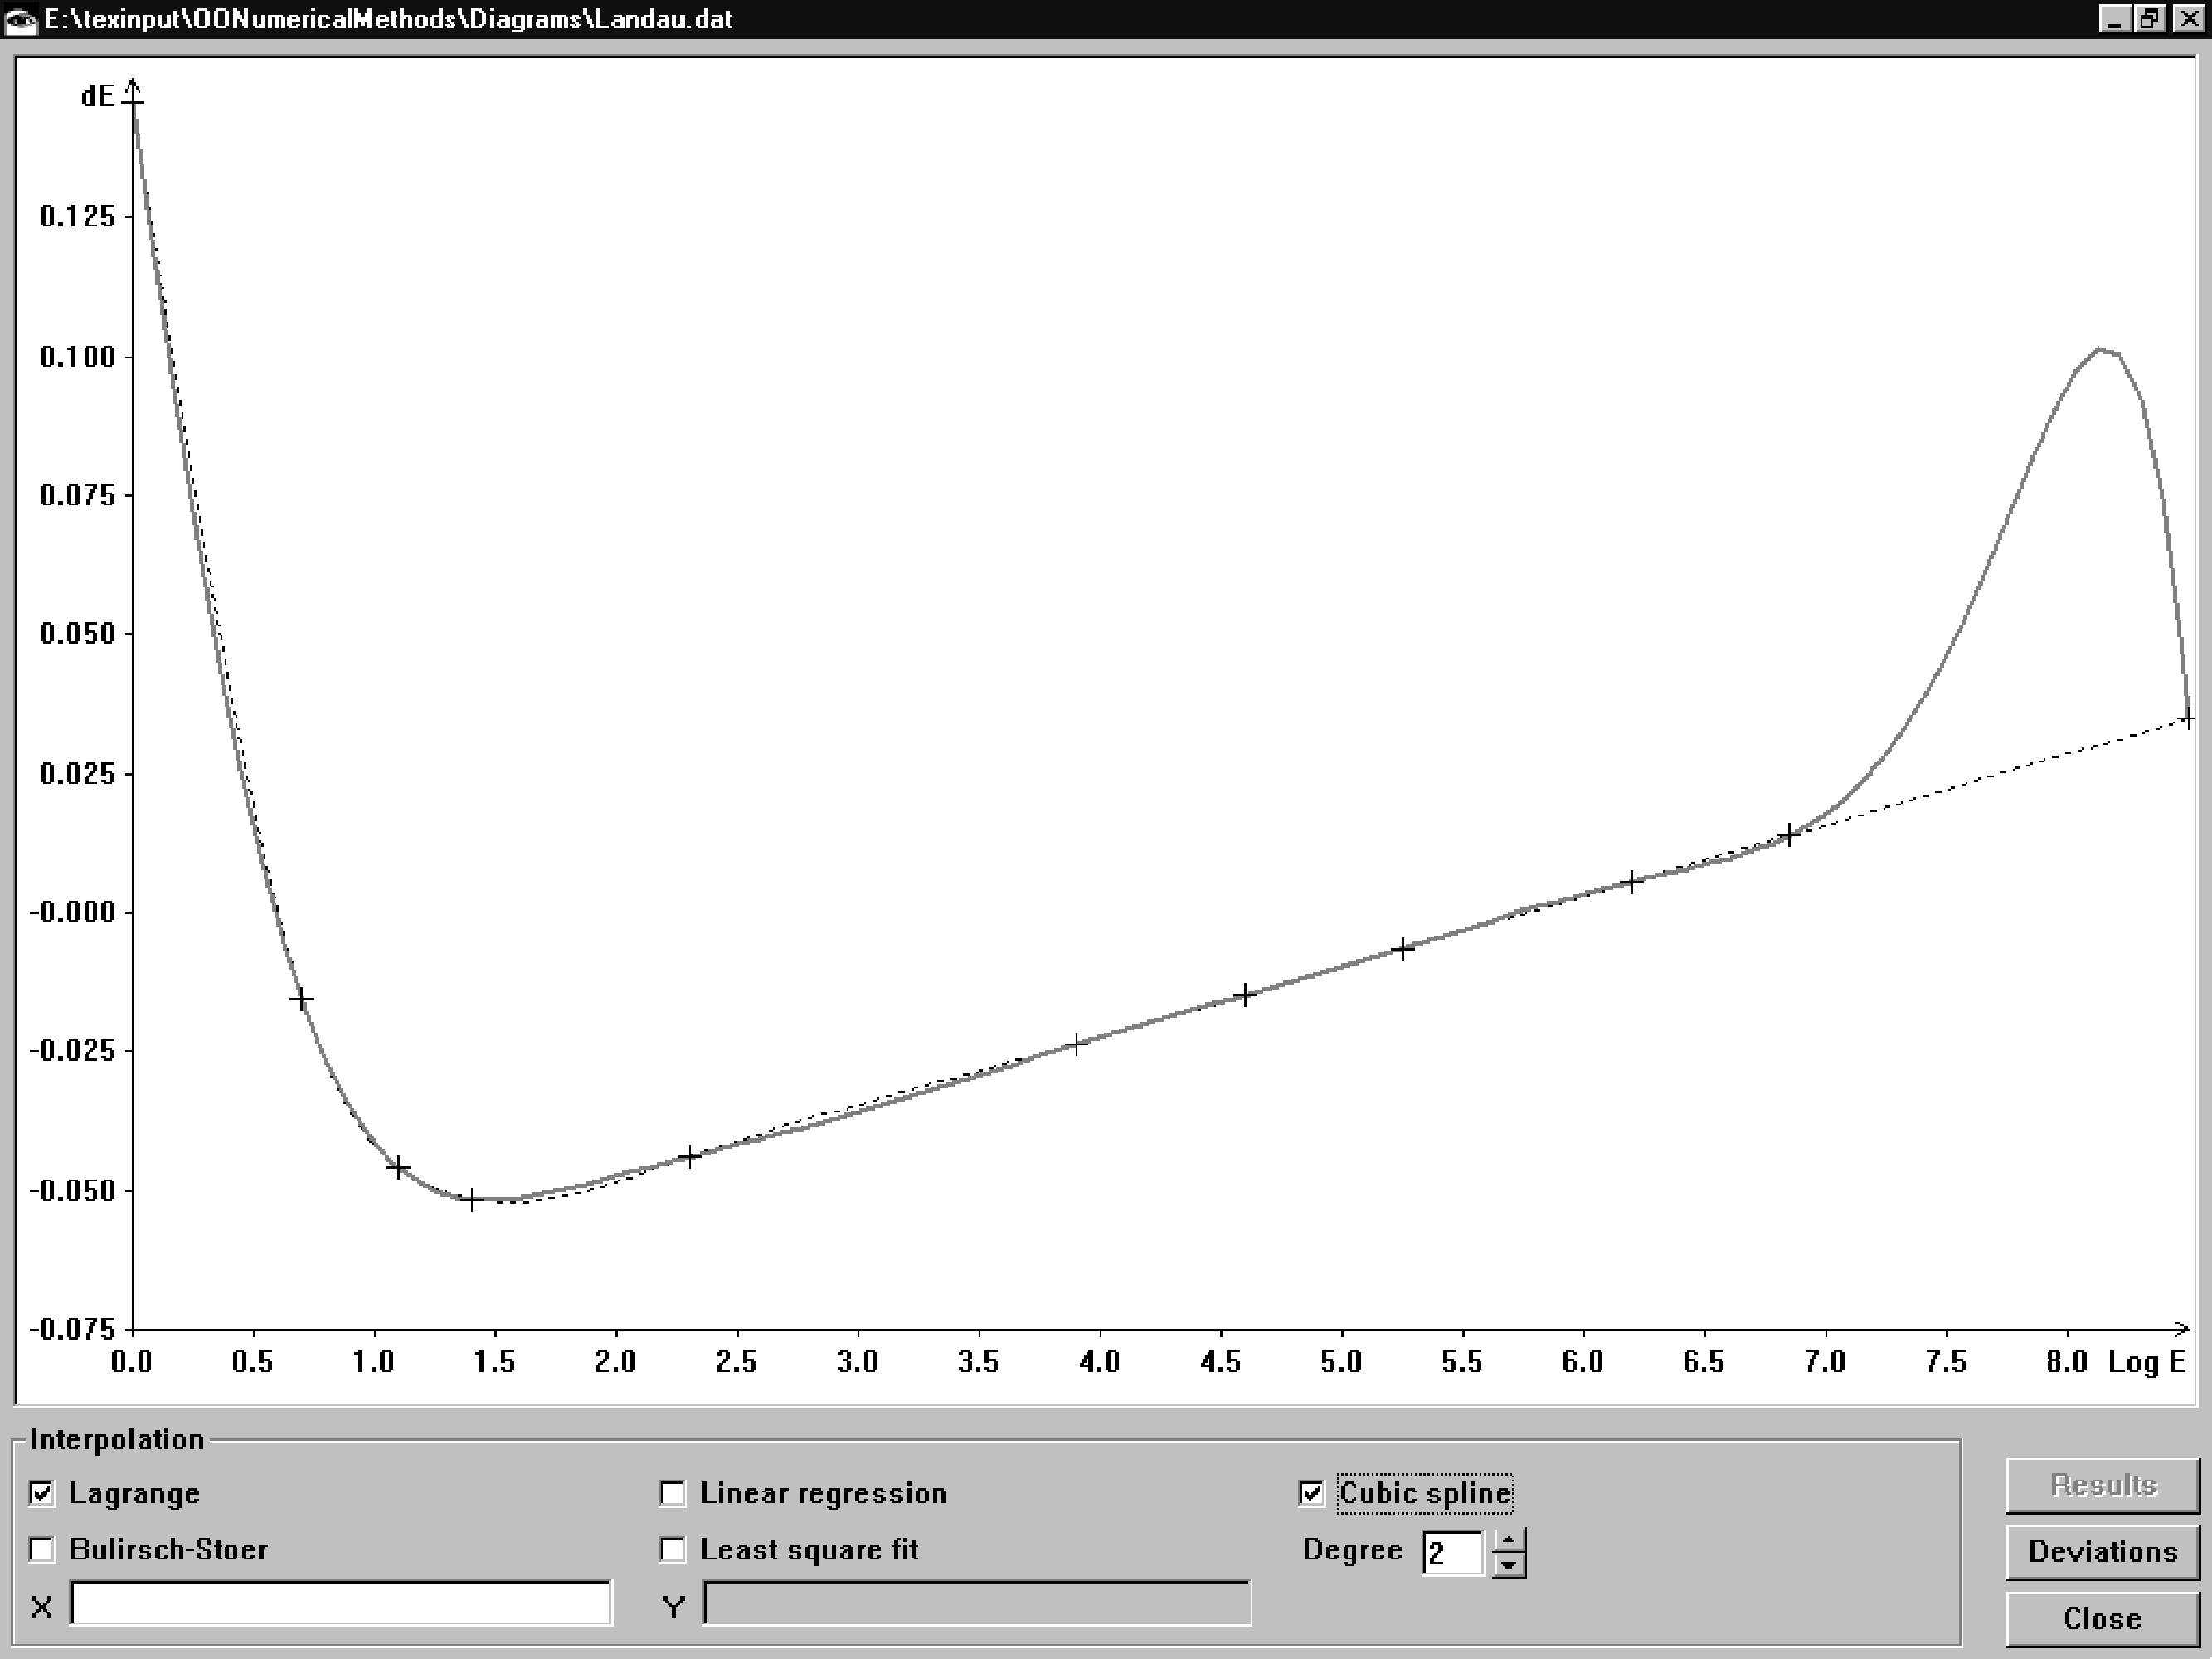
\includegraphics[width=12cm]{Figures/LagrangeVsSpline}
\caption{Comparison of Lagrange interpolation and cubic spline}
\end{figure}
Figure \ref{fig:interpolex3} shows a comparison between the
Lagrange interpolation polynomial (gray thick line) and cubic
spline interpolation (black dotted line) using the same sample
points as in figure \ref{fig:landauinterpol}. The reader can see
that, in the high-energy region (above 4 on the scale of figure
\ref{fig:interpolex2}) the cubic spline does a better job than the
Lagrange polynomial. In fact, since the dependence is linear over
that range, the cubic spline reproduces the theoretical dependence
exactly. In the low energy region, however, cubic spline
interpolation fails to reproduce the curvature of the theoretical
function because of the limitation of the polynomial's degree.

A final example shows a case where interpolation should not be
used. Here the sample points represent the dependence of the
probability that a coin mechanism accepts a wrong coin as a
function of an adjustable threshold. The determination of each
point requires 5-10 minutes of computing time.
\begin{figure}
\label{fig:interpolex4}
\centering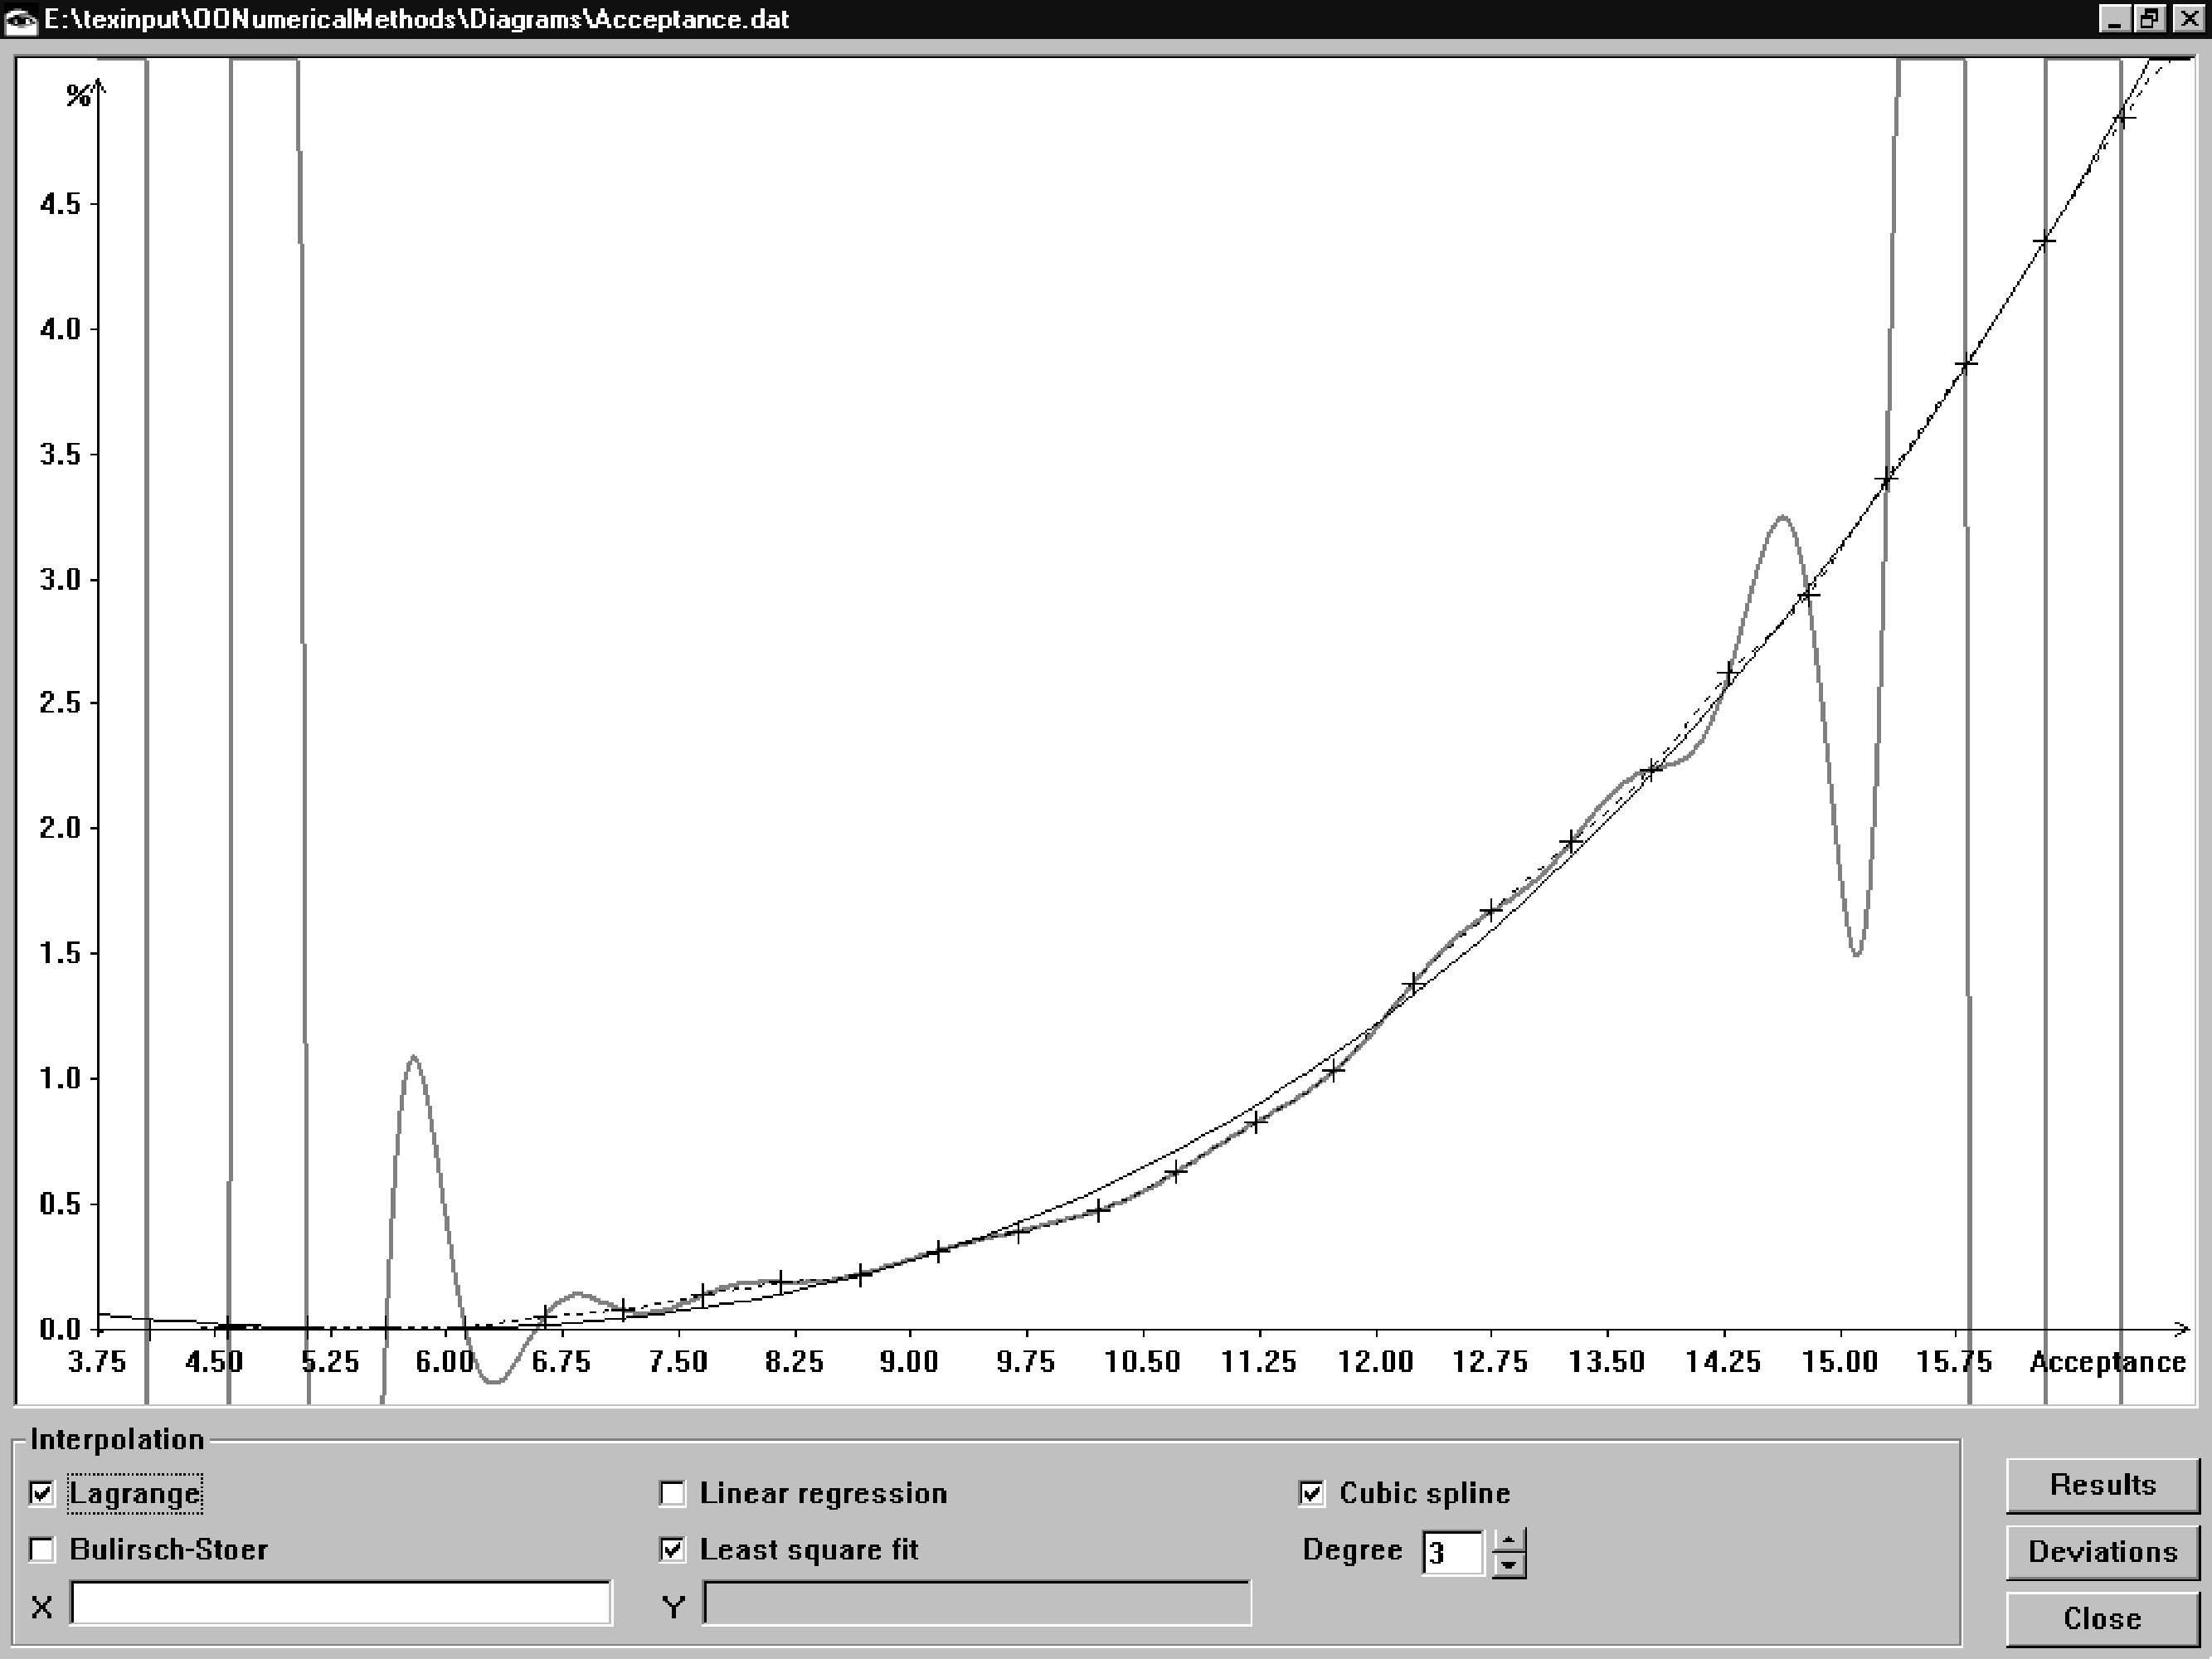
\includegraphics[width=12cm]{Figures/BadInterpolation}
\caption{Example of misbehaving interpolation}
\end{figure}
In this case, however, the simulation was based on using
experimental data. Contrary to the points of figure
\ref{fig:landauinterpol} the points of figure
\ref{fig:interpolex4} are subjected to large fluctuations, because
the sample points have been derived from measured data. Thus,
interpolation does not work.

As in figure \ref{fig:interpolex2}, the gray thick line is the
Lagrange interpolation polynomial and the black dotted line is the
cubic spline. Clearly the Lagrange interpolation polynomial is not
giving any reasonable interpolation. Cubic spline is not really
better as is tries very hard to reproduce the fluctuations of the
computed points. In this case, a polynomial fit (\cf section
\ref{sec:lsfpol}) is the best choice: the thin black line shows
the result of a fit with a $3^{rd}$ degree polynomial.
Another example of unstable interpolation is given in
section \ref{sec:lsfpol} (figure \ref{fig:femurLength}).

\rubrique{Three implementations of Lagrange interpolation} Once
you have verified that a Lagrange interpolation polynomial can be
used to perform reliable interpolation over the sample points, you
must chose among 3 algorithms to compute the Lagrange
interpolation polynomial: direct Lagrange formula, Newton's
algorithm and Neville's algorithm.

Newton's algorithm stores intermediate values which only depends
on the sample points. It is thus recommended, as it is the fastest
method to interpolate several values over the same sample points.
Newton's algorithm is the method of choice to compute a function
from tabulated values.

Neville's algorithm gives an estimate of the numerical error
obtained by the interpolation. It can be used when such
information is needed. Romberg integration, discussed in section
\ref{sec:romberg}, uses Neville's method for that reason.

\section{Lagrange interpolation}
\label{sec:lagrange}
 Let us assume a set of numbers
$x_0,\ldots,x_n$ and the corresponding function's values
$y_0,\ldots,y_n$. There exist a unique polynomial
$P_n\left(x\right)$ of degree $n$ such that
$P_n\left(x_i\right)=y_i$ for all $i=0,\ldots,n$. This polynomial
is the Lagrange interpolation polynomial whose expression is given
by \cite{Knuth2}:
\begin{equation}
\label{eq:lagrange} P_n\left(x\right)=\sum_{i=0}^n{\prod_{j\neq
i}\left(x-x_j\right) \over\prod_{j\neq i}\left(x_i-x_j\right)}y_i.
\end{equation}
For example, the Lagrange interpolation polynomial of degree 2 on
3 points is given by:
\begin{equation}
P_2\left(x\right)={\left(x-x_1\right)\left(x-x_2\right)\over
\left(x_0-x_1\right)\left(x_0-x_2\right)}y_0+{\left(x-x_0\right)\left(x-x_2\right)\over
\left(x_1-x_0\right)\left(x_1-x_2\right)}y_1+{\left(x-x_0\right)\left(x-x_1\right)\over
\left(x_2-x_0\right)\left(x_2-x_1\right)}y_2
\end{equation}

The computation of the polynomial occurs in the order of $\mathcal{O}(n^2)$ since it involves a double iteration.
One can save the evaluation of a few products by rewriting equation \ref{eq:lagrange} as:
\begin{equation}
\label{eq:lagrangesimp}
P_n\left(x\right)=\prod_{i=0}^n\left(x-x_i\right)\sum_{i=0}^n{y_i
\over\left(x-x_i\right)\prod_{j\neq i}\left(x_i-x_j\right)}.
\end{equation}
Of course, equation \ref{eq:lagrangesimp} cannot be evaluated at
the points defining the interpolation. This is easily solved by
returning the defining values as soon as one of the first products
becomes zero during the evaluation.

\subsection{Lagrange interpolation --- Smalltalk implementation}
%\label{sec:slagrange}\marginpar{Figure \ref{cls:interpolation} with the box {\textbf LagrangeInterpolator} grayed.}
The object responsible to implement Lagrange interpolation is defined
uniquely by the sample points over which the interpolation is
performed. In addition it should behave as a function. In other
words it should implement the behavior of a one-variable function
as discussed in section \ref{sec:stFunction}. For example linear
interpolation behaves as follows:

\begin{listing}[label=ex:lagrangeS1]{Smalltalk}
{Linear interpolation}
| interpolator |
interpolator := PMLagrangeInterpolator
                        points: (Array with: 1 @ 2
                                        with: 3 @ 1).
interpolator value: 2.2
\end{listing}

In this example, one creates a new instance of the class \code{PMLagrangeInterpolator} by sending the message \code{points:} to the class \code{PMLagrangeInterpolator} with the collection of
sample points as argument.
The newly created instance is stored in the variable \code{interpolator}.
The next line shows how to compute an interpolated value.

The creation method \code{points:} takes as argument the collection
of sample points. However, it could also accept any object
implementing a subset of the methods of the class \code{Collection}
--- namely the methods \code{size}, \code{at:} and, if we want to be
able to add new sample points, \code{add:}.

One can also spare the creation of an explicit collection object
by implementing these collection methods directly in the Lagrange
interpolation class.
Now, one can also perform interpolation in the following way:

\begin{listing}[label=ex:lagrangeS2]{Smalltalk}
{Alternate way to do a linear interpolation}
| interpolator deviation |
interpolator := PMLagrangeInterpolator new.
1 to: 45 by: 2 do:
                [ :x | interpolator add: x @ (x degreesToRadians sin)].
deviation := (interpolator value: 8) -(8 degreesToRadians sin).
\end{listing}

The code above creates an instance of the class \code{PMLagrangeInterpolator} with an empty collection of sample points. It then adds sample points one by one directly into the
interpolator object. Here the sample points are tabulated values
of the sine function for odd degree values between 1 and 45
degree. The final line of the code compares the interpolated value
with the correct one.

Listing \ref{lst:lagrange} shows the full code of the class
implementing the interface shown above.

The class \code{PMLagrangeInterpolator} is implemented with a
single instance variable containing the collection of sample
points. Each point contains a pair of values
$\left(x_i,y_i\right)$ and is implemented with object of the base
class \code{Point} since an instance of \code{Point} can contain any
type of object in its coordinates. There are two creation methods,
\code{points:} and \code{new}, depending on whether the sample
points are supplied as an explicit object or not. Each creation
method calls in turn an initialization method, respectively \code{initialize:} and \code{initialize}.

The method \code{points:} takes as argument the collection of the
sample points. This object must implement the following methods of
the class \code{Collection}: \code{size}, \code{at:} and \code{add:}.
If the class is created with the method \code{new} an implicit
collection object is created with the method \code{defaultSamplePoints}. This arrangement allows subclasses to select
another type of collection if needed. The default collection
behavior implemented by the class \code{PMLagrangeInterpolator} is
minimal, however. If there is a need for more flexible access to
the collection of sample points, a proper collection object or a
special purpose object should be used.

The interpolation itself is implemented within the single method
\code{value:}. This method is unusually long for object-oriented
programming standards. In this case, however, there is no
compelling reason to split any portion of the algorithm into a
separate method.
Moreover, splitting the method would increase the
computing time.

A final discussion should be made about the two methods \code{xPointAt:} and \code{yPointAt:}.
In principle, there is no need for these methods as the value could be grabbed directly from the collection of points.
If one needs to change the implementation of the point collection in a subclass, however, only these two methods need to be modified.
Introducing this kind of construct can go a long way in program maintenance.

\begin{listing}[label=lst:lagrange]{Smalltalk}
{Smalltalk implementation of the Lagrange interpolation}
Object subclass: #PMLagrangeInterpolator
   instanceVariableNames: 'pointCollection'
   classVariableNames: ''
   package: 'Math-DHB-Numerical-Math-Interpolator'
\end{listing}

\begin{displaycode}{Smalltalk}
PMLagrangeInterpolator class >> new
    ^super new initialize
\end{displaycode}

\begin{displaycode}{Smalltalk}
PMLagrangeInterpolator class >> points: aCollectionOfPoints
    ^self new initialize: aCollectionOfPoints
\end{displaycode}

\begin{displaycode}{Smalltalk}
PMLagrangeInterpolator add: aPoint
    ^pointCollection add: aPoint
\end{displaycode}

\begin{displaycode}{Smalltalk}
PMLagrangeInterpolator >> defaultSamplePoints
    ^OrderedCollection new
\end{displaycode}

\begin{displaycode}{Smalltalk}
PMLagrangeInterpolator >> initialize
    ^self initialize: self defaultSamplePoints
\end{displaycode}

\begin{displaycode}{Smalltalk}
PMLagrangeInterpolator >> initialize: aCollectionOfPoints
    pointCollection := aCollectionOfPoints.
    ^self
\end{displaycode}

\begin{displaycode}{Smalltalk}
PMLagrangeInterpolator >> value: aNumber
    | norm dx products answer size |
    norm := 1.
    size := pointCollection size.
    products := Array new: size.
    products atAllPut: 1.
    1 to: size
        do: [ :n |
              dx := aNumber - ( self xPointAt: n).
              dx = 0
                ifTrue: [ ^( self yPointAt: n)].
              norm := norm * dx.
              1 to: size
                do: [ :m |
                      m = n
                        ifFalse:[ products at: m put: ( (( self 
            xPointAt: m) - ( self xPointAt: n)) * ( products at: m))].
                    ].
            ].
    answer := 0.
    1 to: size do:
        [ :n | answer := ( self yPointAt: n) / ( ( products at: n) * 
                          ( aNumber - ( self xPointAt: n))) + answer].
    ^norm * answer
\end{displaycode}

\begin{displaycode}{Smalltalk}
PMLagrangeInterpolator >> xPointAt: anInteger
    ^( pointCollection at: anInteger) x
\end{displaycode}

\begin{displaycode}{Smalltalk}
PMLagrangeInterpolator >> yPointAt: anInteger
    ^( pointCollection at: anInteger) y
\end{displaycode}

\section{Newton interpolation}
\label{sec:newtoninterpol} If one must evaluate the Lagrange
interpolation polynomial for several values, it is clear that the
Lagrange's formula is not efficient. Indeed a portion of the terms
in the summation of equation \ref{eq:lagrangesimp} depends only on
the sample points and does not depend on the value at which the
polynomial is evaluated. Thus, one can speed up the evaluation of
the polynomial if the invariant parts are computed once and
stored.

If one writes the Lagrange interpolation polynomial using a
generalized Horner expansion, one obtains the Newton's
interpolation formula given by \cite{Knuth2}:
\begin{equation}
\label{eq:newtonhorn}P_n\left(x\right)=\alpha_0+\left(x-x_0\right)\cdot
\left[\alpha_1+\left(x-x_1\right)\cdot\left[\cdots\left[\alpha_{n-1}+\alpha_n\cdot\left(x-x_1\right)\right]\right]\right]
\end{equation}
The coefficients $\alpha_i$ are obtained by evaluating divided
differences as follows:
\begin{equation}
\label{eq:newtoncoef}\left\{ \begin{array}{lcl}\Delta_i^0 &=&y_i
\\ \Delta_i^k &=&{\Delta_i^{k-1}-\Delta_{i-1}^{k-1}\over
x_i-x_{i-k}}\mbox{\quad for $k=1,\ldots,n$}
\\ \alpha_i &=&\Delta_i^i
\end{array}\right.
\end{equation}
Once the coefficients $\alpha_i$ have been obtained, they can be
stored in the object and the generalized Horner expansion of
equation \ref{eq:newtonhorn} can be used.

The time to evaluate the full Newton's algorithm --- that is
computing the coefficients and evaluating the generalized Horner
expansion --- is about twice the time needed to perform a direct
Lagrange interpolation. The evaluation of the generalized Horner
expansion alone, however, has an execution time of $\mathcal{O}(n)$ and
is therefore much faster than the evaluation of a direct Lagrange
interpolation which goes as $\mathcal{O}(n^2)$. Thus, as soon as one needs
to interpolate more than 2 points over the same point sample,
Newton's algorithm is more efficient than direct Lagrange
interpolation.

\subsection{Newton interpolation --- Smalltalk implementation}
%\marginpar{Figure \ref{cls:interpolation} with the box {\textbf NewtonInterpolator} grayed.}
The object implementing Newton's interpolation algorithm is best implemented as a subclass of the
class \code{PMLagrangeInterpolator} because all methods used to
handle the sample points can be reused. This also allows us to
keep the interface identical. It has an additional instance
variable needed to store the coefficients $\alpha_i$. Only 4 new
methods are needed.

Since the client object can add new sample points at will, one
cannot be sure of when it is safe to compute the coefficients.
Thus, computing the coefficients is done with lazy initialization.
The method \code{value:} first checks whether the coefficients
$\alpha_i$ have been computed. If not, the method \code{computeCoefficients} is called. Lazy initialization is a technique
widely used in object oriented programming whenever some value
needs only be computed once.

\noindent The generalized Horner expansion is implemented in the
method \code{value:}.

If a new sample point is added, the coefficient eventually stored
in the object are no longer valid. Thus, the method \code{add:}
first calls the method \code{resetCoefficients} and then calls the
method \code{add:} of the superclass. The method \code{resetCoefficients} makes sure that the coefficients will be
computed anew at the next evaluation of the interpolation
polynomial. The method \code{resetCoefficients} has been
implemented as a separate method so that the reset mechanism can
be reused by any subclass.

Another reason to keep the method \code{resetCoefficients} separate
is that it must also be called before doing an interpolation if
the sample points have been modified directly by the client
application after the last interpolation has been made. An
alternative is to implement the \patstyle{Observable/Observer}
pattern so that resetting of the coefficients happens implicitly
using events. However, since modifying the sample points between
interpolation should only be a rare occasion when using Newton's
algorithm\footnote{If modification of the sample points is not a
rare occasion, then Newton's algorithm has no advantage over
direct Lagrange interpolation or Neville's algorithm. Those
algorithms should be used instead of Newton's algorithm.} our
proposed implementation is much simpler.

Listing \ref{lst:newtonint} shows the complete implementation in
Smalltalk. The class \code{NewtonInterpolator} is a subclass of
class \code{LagrangeInterpolator}. The code examples
\ref{ex:lagrangeS1} and \ref{ex:lagrangeS2} can directly be
applied to Newton interpolation after replacing the class name \code{PMLagrangeInterpolator} with \code{PMNewtonInterpolator}.

The generalized Horner expansion is implemented in the method \code{value:} using explicit indices. One could have used the method \code{inject:into:} as it was done for Horner's formula when
evaluating polynomials. In this case, however, one must still keep
track of the index to retrieve the sample point corresponding to
each coefficient. Thus, one gains very little in compactness.

\begin{listing}[label=lst:newtonint]{Smalltalk}
{Smalltalk implementation of the Newton interpolation}
PMLagrangeInterpolator subclass: #PMNewtonInterpolator
   instanceVariableNames: 'coefficients'
   classVariableNames: ''
   package: 'Math-DHB-Numerical-Math-Interpolator'
\end{listing}

\begin{displaycode}{Smalltalk}
PMNewtonInterpolator >> add: aPoint
    self resetCoefficients.
    ^super add: aPoint
\end{displaycode}

\begin{displaycode}{Smalltalk}
PMNewtonInterpolator >> computeCoefficients
    | size k1 kn|
    size := pointCollection size.
    coefficients := ( 1 to: size) collect: [ :n | self yPointAt: n].
    1 to: (size - 1)
        do: [ :n |
              size to: ( n + 1)  by: -1
                do: [ :k |
                      k1 := k - 1.
                      kn := k - n.
                      coefficients at: k put: ( (( coefficients at: 
                                         k) - ( coefficients at: k1)) 
                                            / ((self xPointAt: k) - 
                                                (self xPointAt: kn))).
                    ].
            ].
\end{displaycode}

\begin{displaycode}{Smalltalk}
PMNewtonInterpolator >> resetCoefficients
    coefficients := nil.
\end{displaycode}

\begin{displaycode}{Smalltalk}
PMNewtonInterpolator >> value: aNumber
    | answer size |
    coefficients isNil
        ifTrue: [ self computeCoefficients].
    size := coefficients size.
    answer := coefficients at: size.
    (size - 1) to: 1 by: -1
        do: [ :n | answer := answer * ( aNumber - (self xPointAt:  
                                         n)) + ( coefficients at: n)].
    ^answer
\end{displaycode}

\section{Neville interpolation}
\label{sec:neville} Neville's algorithm uses a successive
approximation approach implemented in practice by calculating
divided differences recursively. The idea behind the algorithm is
to compute the value of the interpolation's polynomials of all
degrees between 0 and $n$. This algorithm assumes that the sample
points have been sorted in increasing order of abscissa.

Let $P^i_j\left(x\right)$ be the (partial) Lagrange interpolation
polynomials of degree $i$ defined by the sets of values
$x_j,\ldots,x_{j+i}$ and the corresponding function's values
$y_j,\ldots,y_{j+i}$. From equation \ref{eq:lagrange} one can
derive the following recurrence formula \cite{Press}:
\begin{equation}
\label{eq:neville}
P^i_j\left(x\right)={\left(x-x_{i+j}\right)P^{i-1}_j\left(x\right)
+\left(x_j-x\right)P^{i-1}_{j+1}\left(x\right)\over x_j-x_{i+j}}
\mbox{\quad for $j<i$}.
\end{equation}
The initial values $P^0_j\left(x\right)$ are simply $y_j$. The
value of the final Lagrange's polynomial is $P^n_0\left(x\right)$.

Neville's algorithm introduces the differences between the
polynomials of various degrees. One defines:
\begin{equation}
\left\{ \begin{array}{lcl} \Delta_{j,i}^{\mathop
{left}}\left(x\right)
&=&P^i_j\left(x\right)-P^{i-1}_j\left(x\right)
\\*[3 ex] \Delta_{j,i}^{\mathop{right}}\left(x\right) &=&P^i_j\left(x\right)-P^{i-1}_{j+1}\left(x\right)
\end{array}\right.
\end{equation}
From the definition above and equation \ref{eq:neville} one
derives a pair of recurrence formulae for the differences:
\begin{equation}
\left\{ \begin{array}{lcl}\Delta_{j,i+1}^{\mathop
{left}}\left(x\right) &=&{x_i-x\over
x_j-x_{i+j+1}}\left(\Delta_{j+1,i}^{\mathop
{left}}\left(x\right)-\Delta_{j,i}^{\mathop
{right}}\left(x\right)\right)
\\*[3 ex] \Delta_{j,i+1}^{\mathop{right}} &=&{x_{i+j+1}-x\over
x_j-x_{i+j+1}}\left(\Delta_{j+1,i}^{\mathop
{left}}\left(x\right)-\Delta_{j,i}^{\mathop
{right}}\left(x\right)\right)
\end{array}\right.
\end{equation}
In practice two arrays of differences --- one for left and one for
right --- are allocated. Computation of each order is made within
the same arrays. The differences of the last order can be
interpreted as an estimation of the error made in replacing the
function by the interpolation's polynomial.

Neville's algorithm is faster than the evaluation of direct
Lagrange's interpolation for a small number of points (smaller
than about 7\footnote{\cf footnote \ref{ft:lagnev} on page
\pageref{ft:lagnev}}. Therefore a simple linear interpolation is
best performed using Neville's algorithm. For a large number of
points, it becomes significantly slower.

\subsection{ Neville interpolation --- Smalltalk  implementation}
%\marginpar{Figure \ref{cls:interpolation} with the box {\textbf NevilleInterpolator} grayed.}
The object implementing Neville's interpolation's algorithm is best implemented as a subclass of the
class \code{LagrangeInterpolator} since the methods used to handle
the sample points can be reused. This also allows us to keep the
interface identical.

The new class has two additional instance variables used to store
the finite differences $\Delta_{j,i}^{\mathop{
left}}\left(x\right)$ and $\Delta_{j,i}^{\mathop{
right}}\left(x\right)$ for all $j$.
These instance variables are recycled for all $i$.
Only a few additional methods are needed.

The method \code{valueAndError:} implementing Neville's algorithm
returns an array with two elements: the first element is the
interpolated value and the second is the estimated error. The
method \code{value:} calls the former method and returns only the
interpolated value.

Unlike other interpolation algorithms, the method \code{valueAndError:} is broken into smaller methods because the
mechanics of computing the finite differences will be reused in
the Bulirsch-Stoer algorithm. The method \code{valueAndError:}
begins by calling the method \code{initializeDifferences:} to
populate the arrays containing the finite differences with their
initial values. These arrays are created if this is the first time
they are used with the current sample points. This prevents
unnecessary memory allocation. Then, at each iteration the method \code{computeDifference:at:order:} computes the differences for the current order.

Listing \ref{lst:neville} shows the implementation of Neville's
algorithm in Smalltalk. The class \code{PMNevilleInterpolator} is
a subclass of class \code{PMLagrangeInterpolator}. The code
examples \ref{ex:lagrangeS1} and \ref{ex:lagrangeS2} can directly
be applied to Neville interpolation after replacing the class name
\code{PMLagrangeInterpolator} with \code{PMNevilleInterpolator}.
An example of interpolation using the returned estimated error is
given in section \ref{sec:sromberg}.

The method \code{defaultSamplePoints} overrides that of the
superclass to return a sorted collection. Thus, each point added
to the implicit collection is automatically sorted by increasing
abscissa as required by Neville's algorithm.

\begin{listing}[label=lst:neville]{Smalltalk}
{Smalltalk implementation of Neville's algorithm}
PMLagrangeInterpolator subclass: #PMNevilleInterpolator
   instanceVariableNames: 'leftErrors rightErrors'
   classVariableNames: ''
   package: 'Math-DHB-Numerical-Math-Interpolator'
\end{listing}

\begin{displaycode}{Smalltalk}
PMNevilleInterpolator >> computeDifference: aNumber at: anInteger1 order: anInteger2
    | leftDist rightDist ratio |
    leftDist := ( self xPointAt: anInteger1) - aNumber.
    rightDist := (  self xPointAt: ( anInteger1 + anInteger2)) - 
                                                              aNumber.
    ratio := ( ( leftErrors at: ( anInteger1 + 1)) - ( rightErrors 
                           at: anInteger1)) / ( leftDist - rightDist).
    leftErrors at: anInteger1 put: ratio * leftDist.
    rightErrors at: anInteger1 put: ratio * rightDist.
\end{displaycode}

\begin{displaycode}{Smalltalk}
PMNevilleInterpolator >> defaultSamplePoints
    ^SortedCollection sortBlock: [ :a :b | a x < b x]
\end{displaycode}

\begin{displaycode}{Smalltalk}
PMNevilleInterpolator >> initializeDifferences: aNumber
    | size nearestIndex dist minDist |
    size := pointCollection size.
    leftErrors size = size
        ifFalse:[ leftErrors := Array new: size.
                  rightErrors := Array new: size.
                ].
    minDist := ( ( self xPointAt: 1) - aNumber) abs.
    nearestIndex := 1.
    leftErrors at: 1 put: ( self yPointAt: 1).
    rightErrors at: 1 put: leftErrors first.
    2 to: size do:
        [ :n |
          dist := ( ( self xPointAt: n) - aNumber) abs.
          dist < minDist
            ifTrue: [ dist = 0
                        ifTrue: [ ^n negated].
                      nearestIndex := n.
                      minDist := dist.
                    ].
         leftErrors at: n put: ( self yPointAt: n).
         rightErrors at: n put: ( leftErrors at: n).
        ].
    ^nearestIndex
\end{displaycode}

\begin{displaycode}{Smalltalk}
PMNevilleInterpolator >> value: aNumber
    ^(self valueAndError: aNumber) first
\end{displaycode}

\begin{displaycode}{Smalltalk}
PMNevilleInterpolator >>valueAndError: aNumber
    | size nearestIndex answer error |
    nearestIndex := self initializeDifferences: aNumber.
    nearestIndex < 0
        ifTrue: [ ^Array with: ( self yPointAt: nearestIndex negated) 
                                                             with: 0].
    answer := leftErrors at: nearestIndex.
    nearestIndex := nearestIndex - 1.
    size := pointCollection size.
    1 to: ( size - 1) do:
        [ :m |
          1 to: ( size - m) do:
            [ :n | self computeDifference: aNumber at: n order: m].
          size - m > ( 2 * nearestIndex)
                ifTrue: [ error := leftErrors at: ( nearestIndex + 1) 
                                                                     ]
                ifFalse:[ error := rightErrors at: ( nearestIndex).
                              nearestIndex := nearestIndex - 1.
                            ].
          answer := answer + error.
        ].
    ^Array with: answer with: error abs

\end{displaycode}

\section{Bulirsch-Stoer interpolation}
If the function to interpolate is known to have
poles\footnote{That is, a singularity in the complex plane.} in
the vicinity of the real axis over the range of the sample points
a polynomial cannot do a good interpolation job \cite{Press}.

In this case it is better to use rational function, that is a
quotient of two polynomials as defined hereafter:
\begin{equation}
R\left(x\right)={P\left(x\right)\over Q\left(x\right)}
\end{equation}
The coefficients of both polynomials are only defined up to a
common factor. Thus, if $p$ is the degree of polynomial
$P\left(x\right)$ and $q$ is the degree of polynomial
$Q\left(x\right)$, we must have the relation $p+q+1 = n$ where $n$
is the number of sample points. This of course is not enough to
restrict the variety of possible rational functions.

Bulirsch and Stoer have proposed an algorithm for a rational
function where $p=\lfloor{n-1 \over 2}\rfloor$. This means that
$q$ is either equal to $p$ if the number of sample points is odd
or equal to $p+1$ if the number of sample points is even. Such a
rational function is called a diagonal rational function. This
restriction, of course, limits the type of function shapes that
can be interpolated.

The Bulirsch-Stoer algorithm is constructed like Neville's
algorithm: finite differences are constructed until all points
have been taken into account.

Let $R_j^i\left(x\right)$ be the (partial) diagonal rational
functions of order $i$ defined by the sets of values
$x_j,\ldots,x_{j+i}$ and the corresponding function's values
$y_j,\ldots,y_{j+i}$. As in the case of Neville's algorithm, one
can establish a recurrence formula between functions of successive
orders. We have \cite{Press}:
\begin{equation}
\label{eq:bustoer}
R_j^i\left(x\right)=R_{j+1}^{i-1}\left(x\right)+
{R_{j+1}^{i-1}\left(x\right) - R_j^{i-1}\left(x\right) \over
{x-x_j\over x-x_{i+j}}\left(1-{R_{j+1}^{i-1}\left(x\right)
-R_j^{i-1}\left(x\right)\over R_{j+1}^{i-1}\left(x\right)
-R_{j+1}^{i-2}\left(x\right)}\right)}\mbox{\quad for $j<i$}.
\end{equation}
The initial values $R_j^0\left(x\right)$ are simply $y_j$. The
final rational function is $R_0^n\left(x\right)$.

Like in Neville's algorithm one introduces the differences between
the functions of various orders. One defines:
\begin{equation}
\left\{
\begin{array}{lcl}
    \Delta_{j,i}^{\mathop{\textrm
left}}\left(x\right) & = & R_j^i\left(x\right) -
R_j^{i-1}\left(x\right)\\*[2ex]
    \Delta_{j,i}^{\mathop{\textrm
right}}\left(x\right) & = & R_j^j\left(x\right) -
R_{j+1}^{i-1}\left(x\right)
  \end{array}\right.
\end{equation}
From the definition above and equation \ref{eq:bustoer} one
derives a pair of recurrence formulae for the differences:
\begin{equation}
\left\{
\begin{array}{lcl}
    \Delta_{j,i+1}^{\mathop{\textrm
left}}\left(x\right) & = &{{x-x_j \over x - x_{i+j+1}}
\Delta_{j,i}^{\mathop{\textrm right}}\left(x\right)
\left[\Delta_{j+1,i}^{\mathop{\textrm left}}\left(x\right) -
\Delta_{j,i}^{\mathop{\textrm right}}\left(x\right)\right] \over
{x-x_j \over x-x_{i+j+1}} \Delta_{j,i}^{\mathop{\textrm
right}}\left(x\right) - \Delta_{j+1,i}^{\mathop{\textrm
left}}\left(x\right)}
\\*[3ex]
    \Delta_{j,i}^{\mathop{\textrm
right}}\left(x\right) & = &{ \Delta_{j+1,i}^{\mathop{\textrm
left}}\left(x\right) \left[\Delta_{j+1,i}^{\mathop{\textrm
left}}\left(x\right) - \Delta_{j,i}^{\mathop{\textrm
right}}\left(x\right)\right] \over {x-x_j \over x-x_{i+j+1}}
\Delta_{j,i}^{\mathop{\textrm right}}\left(x\right) -
\Delta_{j+1,i}^{\mathop{\textrm left}}\left(x\right)}
  \end{array}\right.
\end{equation}
Like for Neville's algorithm, two arrays of differences --- one
for left and one for right --- are allocated. Computation of each
order is made within the same arrays. The differences of the last
order can be interpreted as an estimation of the error made in
replacing the function by the interpolating rational function.
Given the many similarities with Neville's algorithm many methods
of that algorithm can be reused.

\subsection{Bulirsch-Stoer interpolation --- Smalltalk implementation}

%\marginpar{Figure \ref{cls:interpolation} with the box {\textbf BulirschStoerInterpolator} grayed.}
The object implementing Bulirsch-Stoer interpolation's algorithm is best implemented as a
subclass of the class \code{PMNevilleInterpolator} since the
methods used to manage the computation of the finite differences
can be reused. The public interface is identical.

Only a single method --- the one responsible for the evaluation of
the finite differences at each order --- must be implemented. All
other methods of Neville's interpolation can be reused.

This shows the great power of object-oriented approach. Code
written in procedural language cannot be reused that easily. In
\cite{Press} the two codes implementing Neville's and
Bulirsch-Stoer interpolation are of comparable length; not
surprisingly they also have much in common.

Listing \ref{lst:bustoer} shows the implementation of
Bulirsch-Stoer interpolation in Smalltalk. The class \code{PMBulirschStoerInterpolator} is a subclass of class \code{PMNevilleInterpolator}. The code examples \ref{ex:lagrangeS1} and
\ref{ex:lagrangeS2} can directly be applied to Bulirsch-Stoer
interpolation after replacing the class name \code{PMLagrangeInterpolator} with \code{PMBulirschStoerInterpolator}.

\begin{listing}[label=lst:bustoer]{Smalltalk}
{Smalltalk implementation of Bulirsch-Stoer interpolation}
PMNevilleInterpolator subclass: #PMBulirschStoerInterpolator
   instanceVariableNames: ''
   classVariableNames: ''
   package: 'Math-DHB-Numerical-Math-Interpolator'
\end{listing}

\begin{displaycode}{Smalltalk}
PMBulirschStoerInterpolator >> computeDifference: aNumber at: anInteger1 order: anInteger2
    | diff ratio |
    ratio := ( ( self xPointAt: anInteger1) - aNumber) * ( 
                                           rightErrors at: anInteger1)
                            / ( (  self xPointAt: ( anInteger1 + 
                                              anInteger2)) - aNumber).
    diff := ( ( leftErrors at: ( anInteger1 + 1)) - ( rightErrors at: 
                                                          anInteger1))
                            / ( ratio - ( leftErrors at: ( anInteger1 
                                                               + 1))).
    rightErrors at: anInteger1 put: ( leftErrors at: ( anInteger1 + 
                                                          1)) * diff. 
    leftErrors at: anInteger1 put: ratio * diff.
\end{displaycode}

\section{Cubic spline interpolation}
The Lagrange interpolation polynomial is defined globally over the
set of given points and respective function's values. As we have
seen in figure \ref{fig:interpolex4} and to a lesser degree in
figure \ref{fig:interpolex3} Lagrange's interpolation polynomial
can have large fluctuations between two adjacent points because
the degree of the interpolating polynomial is not constrained.

One practical method for interpolating a set of function's value
with a polynomial of constrained degree is to use cubic splines. A
cubic spline is a $3^{\mathop{\textrm rd}}$ order polynomial
constrained in its derivatives at the end points. A unique cubic
spline is defined for each interval between two adjacent points.
The interpolated function is required to be continuous up to the
second derivative at each of the points.

Before the advent of computers, people were drawing smooth curves
by sticking nails at the location of computed points and placing
flat bands of metal between the nails. The bands were then used as
rulers to draw the desired curve. These bands of metal were called
splines and this is where the name of the interpolation algorithm
comes from. The elasticity property of the splines correspond to
the continuity property of the cubic spline function.

The algorithm exposed hereafter assumes that the sample points
have been sorted in increasing order of abscissa.

To derive the expression for the cubic spline, one first assumes
that the second derivatives of the splines, $y^{\prime\prime}_i$,
are known at each point. Then one writes the cubic spline between
$x_{i-1}$ and $x_i$ in the following symmetric form:
\begin{equation}
\label{eq:splinedef} P_i\left(x\right)=y_{i-1}A_i\left(x\right) +
y_i B_i\left(x\right) + y^{\prime\prime}_{i-1}C_i\left(x\right) +
y^{\prime\prime}_i D_i\left(x\right),
\end{equation}
where
\begin{equation}
\label{eq:splinelin}  \left\{
  \begin{array}{lcl}
    A_i\left(x\right) & = & \displaystyle x_i - x \over\displaystyle x_i - x_{i-1}, \\*[2 ex]
    B_i\left(x\right) & = & \displaystyle x - x_{i-1} \over\displaystyle x_i - x_{i-1}.
  \end{array}\right.
\end{equation}
Using the definition above, the first two terms in equation
\ref{eq:splinedef} represents the linear interpolation between the
two points $x_{i-1}$ and $x_i$. Thus, the last two terms of must
vanish at $x_{i-1}$ and $x_i$. In addition we must have by
definition:
\begin{equation}
\label{eq:splinedifeq}
 \left\{
  \begin{array}{lcl}
    \left.{\displaystyle d^2P_i\left(x\right)\over\displaystyle dx^2}\right|_{x=x_{i-1}} & = &
    y^{\prime\prime}_{i-1},
    \\*[3 ex]
    \left.{\displaystyle d^2P_i\left(x\right)\over\displaystyle dx^2}\right|_{x=x_i} & = &
    y^{\prime\prime}_i.
  \end{array} \right.
\end{equation}
One can rewrite the first equation in \ref{eq:splinedifeq} as a
differential equation for the function $C_i$ as a function of
$A_i$. Similarly, the second equation is rewritten as a
differential equation for the function $D_i$ as a function of
$B_i$. This yields:
\begin{equation}
\label{eq:splinecub}
 \left\{
  \begin{array}{lcl}
    C_i\left(x\right) & = &
    {\displaystyle A_i\left(x\right)\left[A_i\left(x\right)^2-1\right]\over\displaystyle 6} \left(x_i - x_{i-1}\right)^2,
    \\*[3 ex]
    D_i\left(x\right) & = &
    {\displaystyle B_i\left(x\right)\left[B_i\left(x\right)^2-1\right]\over\displaystyle 6} \left(x_i - x_{i-1}\right)^2,
  \end{array} \right.
\end{equation}
Finally, one must use the fact that the first derivatives of each
spline must be equal at each end points of the interval, that is:
\begin{equation}
 {dP_i\left(x\right)\over dx}={dP_{i+1}\left(x\right)\over dx}.
\end{equation}
This yields the following equations for the second derivatives
$y^{\prime\prime}_i$:
\begin{equation}
\label{eq:splinesyst}
  {x_{i+1}-x_i \over 6}y^{\prime\prime}_{i+1}
  + {x_{i+1}-x_{i-1} \over  6}y^{\prime\prime}_i
  + {x_i-x_{i-1} \over 6}y^{\prime\prime}_{i-1}=
  {y_{i+1}-y_i \over x_{i+1}-x_i} - {y_i-y_{i-1} \over  x_i-x_{i-1}}.
\end{equation}
There are $n-1$ equations for the $n$ unknowns
$y^{\prime\prime}_i$. We are thus missing two equations. There are
two ways of defining two additional equations to obtain a unique
solution.
\begin{itemize}
  \item The first method is the so-called natural cubic spline for which
one sets $y^{\prime\prime}_0=y^{\prime\prime}_n=0$. This means
that the spline is flat at the end points.
  \item The second method is called constrained cubic spline. In this case the
first derivatives of the function at $x_0$ and $x_n$,
$y^{\prime}_0$ and $y^{\prime}_n$, are set to given values.
\end{itemize}

In the case of constrained cubic spline, one obtain two additional
equations by evaluating the derivatives of equation
\ref{eq:splinedef} at $x_0$ and $x_n$:
\begin{equation}
\label{eq:splineend}
 \left\{
  \begin{array}{lcl}
    {3A_1\left(x\right)^2-1\over 6}\left(x_1-x_0\right) y^{\prime\prime}_0 -
    {3B_1\left(x\right)^2-1\over 6}\left(x_1-x_0\right) y^{\prime\prime}_1 & = &
    y^{\prime}_0 - {y_1-y_0 \over x_1-x_0},
    \\*[3 ex]
    {3A_n\left(x\right)^2-1\over 6}\left(x_n-x_{n-1}\right) y^{\prime\prime}_n -
    {3B_n\left(x\right)^2-1\over 6}\left(x_n-x_{n-1}\right) y^{\prime\prime}_{n-1} & = &
    y^{\prime}_n - {y_n-y_{n-1} \over x_n-x_{n-1}}.
  \end{array} \right.
\end{equation}
The choice between natural or constrained spline can be made
independently at each end point.

One solves the system of equations \ref{eq:splinesyst}, and
possibly \ref{eq:splineend}, using direct Gaussian elimination and
back substitution (\cf section \ref{sec:lineqs}). Because the
corresponding matrix is tridiagonal, each pivoting step only
involves one operation. Thus, resorting to a general algorithm for
solving a system of linear equations is not necessary.

\subsection{Cubic spline interpolation --- Smalltalk  implementation}
%\marginpar{Figure \ref{cls:interpolation} with the box {\textbf SplineInterpolator} grayed.}
In both languages the object implementing cubic spline interpolation is a subclass of the
Newton interpolator. The reader might be surprised by this choice
since, mathematically speaking, these two objects do not have
anything in common.

However, from the behavioral point of view, they are quite
similar. Like for Newton interpolation, cubic spline interpolation
first needs to compute a series of coefficients, namely the second
derivatives, which only depends on the sample points. This
calculation only needs to be performed once. Then the evaluation
of the function can be done using equations \ref{eq:splinedef},
\ref{eq:splinelin} and \ref{eq:splinecub}. Finally, as for the
Newton interpolator, any modification of the points requires a new
computation of the coefficients. The behavior can be reused from
the class \code{NewtonInterpolator}.

The second derivatives needed by the algorithm are stored in the
variable used to store the coefficients of Newton's algorithm.

The class \code{SplineInterpolator} has two additional instance
variables needed to store the end point derivatives $y^{\prime}_0$
and $y^{\prime}_n$. Corresponding methods needed to set or reset
these values are implemented. If the value of $y^{\prime}_0$ or
$y^{\prime}_n$ is changed then the coefficients must be reset.

Natural or constrained cubic spline is flagged independently at
each point by testing if the corresponding end-point derivative
has been supplied or not. The second derivatives are computed used
lazy initialization by the method \code{computeSecondDerivatives}.

Listing \ref{lst:spline} shows the implementation of cubic spline
interpolation in Smalltalk. The class \code{PMSplineInterpolator}
is a subclass of class \code{PMNewtonInterpolator}. The code
examples \ref{ex:lagrangeS1} and \ref{ex:lagrangeS2} can directly
be applied to cubic spline interpolation after replacing the class
name \code{PMLagrangeInterpolator} with \code{PMSplineInterpolator}.

If the end-point derivative is \code{nil} the corresponding
end-point is treated as a natural spline.

The method \code{defaultSamplePoints} overrides that of the
superclass to create a sorted collection. Thus, as each point is
added to the implicit collection, the collection of sample points
remains in increasing order of abscissa as required by the cubic
spline algorithm.

\begin{listing}[label=lst:spline]{Smalltalk}
{Smalltalk implementation of cubic spline interpolation}
PMNewtonInterpolator subclass: #PMSplineInterpolator
   instanceVariableNames: 'startPointDerivative endPointDerivative'
   classVariableNames: ''
   package: 'Math-DHB-Numerical-Math-Interpolator'
\end{listing}

\begin{displaycode}{Smalltalk}
PMSplineInterpolator >> computeSecondDerivatives
    | size u w s dx inv2dx |
    size := pointCollection size.
    coefficients := Array new: size.
    u := Array new: size - 1.
    startPointDerivative isNil 
        ifTrue: 
            [coefficients at: 1 put: 0.
            u at: 1 put: 0]
        ifFalse: 
            [coefficients at: 1 put: -1 / 2.
            s := 1 / (( self xPointAt: 2) x - ( self xPointAt: 1) x).
            u at: 1
                put: 3 * s 
                        * (s * (( self yPointAt: size) - ( self 
                                                 yPointAt: size - 1)) 
                                - startPointDerivative)].
    2 to: size - 1
        do: 
            [:n | 
            dx := (self xPointAt: n) - (self xPointAt: ( n - 1)).
            inv2dx := 1 / (( self xPointAt: n + 1) - (self xPointAt: 
                                                              n - 1)).
            s := dx * inv2dx.
            w := 1 / (s * (coefficients at: n - 1) + 2).
            coefficients at: n put: (s - 1) * w.
            u at: n
                put: (((( self yPointAt: n + 1) - ( self yPointAt: 
                                                                  n)) 
                        / (( self xPointAt: n + 1) - ( self xPointAt: 
                                                                  n)) 
                            - ((( self yPointAt: n) - ( self 
                                         yPointAt: n - 1)) / dx)) * 6 
                        * inv2dx - ((u at: n - 1) * s)) 
                        * w].
    endPointDerivative isNil 
        ifTrue: [coefficients at: size put: 0]
        ifFalse: 
            [w := 1 / 2.
            s := 1 / ((self xPointAt:  size) - (self xPointAt: ( size 
                                                               - 1))).
            u at: 1
                put: 3 * s * (endPointDerivative 
                                - (s * (self yPointAt: size) - (self 
                                                yPointAt: size - 1))).
            coefficients at: size
                put: s - (w * (u at: size - 1) / ((coefficients at: 
                                                 size - 1) * w + 1))].
    size - 1 to: 1
        by: -1
        do: 
            [:n | 
            coefficients at: n
                put: (coefficients at: n) * (coefficients at: n + 1) 
                                                          + (u at: n)]

\end{displaycode}

\begin{displaycode}{Smalltalk}
PMSplineInterpolator >> defaultSamplePoints
    ^SortedCollection sortBlock: [ :a :b | a x < b x]
\end{displaycode}

\begin{displaycode}{Smalltalk}
PMSplineInterpolator >> endPointDerivative: aNumber
    endPointDerivative := aNumber.
    self resetCoefficients
\end{displaycode}

\begin{displaycode}{Smalltalk}
PMSplineInterpolator >> resetEndPointDerivatives
    self setEndPointDerivatives: ( Array new: 2)
\end{displaycode}

\begin{displaycode}{Smalltalk}
PMSplineInterpolator >> setEndPointDerivatives: anArray
    startPointDerivative := anArray at: 1.
    endPointDerivative := anArray at: 2.
    self resetCoefficients
\end{displaycode}

\begin{displaycode}{Smalltalk}
PMSplineInterpolator >> startPointDerivative: aNumber
    startPointDerivative := aNumber.
    self resetCoefficients
\end{displaycode}

\begin{displaycode}{Smalltalk}
PMSplineInterpolator >> value: aNumber
    | answer n1 n2 n step a b |
    coefficients isNil ifTrue: [self computeSecondDerivatives].
    n2 := pointCollection size.
    n1 := 1.
    [n2 - n1 > 1] whileTrue: 
            [n := (n1 + n2) // 2.
            (self xPointAt:  n) > aNumber ifTrue: [n2 := n] ifFalse: 
                                                           [n1 := n]].
    step := (self xPointAt: n2) - (self xPointAt: n1).
    a := ((self xPointAt: n2) - aNumber) / step.
    b := (aNumber - (self xPointAt: n1)) / step.
    ^a * (self yPointAt: n1) + (b * (self yPointAt: n2)) 
        + ((a * (a squared - 1) * (coefficients at: n1) 
                + (b * (b squared - 1) * (coefficients at: n2))) * 
                                                         step squared 
                / 6)
\end{displaycode}

\section{Which method to choose?}
At this point some reader might experience some difficulty in
choosing among the many interpolation algorithms discussed in this
book. There are indeed many ways to skin a cat. Selecting a method
depends on what the user intends to do with the data.

First of all, the reader should be reminded that Lagrange
interpolation, Newton interpolation and Neville's algorithm are
different algorithms computing the values of the same function,
namely the Lagrange interpolation polynomial. In other words, the
interpolated value resulting from each 3 algorithms is the same
(up to rounding errors of course).

The Lagrange interpolation polynomial can be subject to strong
variations (if not wild in some cases, figure
\ref{fig:interpolex4} for example) if the sampling points are not
smooth enough. A cubic spline may depart from the desired function
if the derivatives on the end points are not constrained to proper
values. A rational function can do a good job in cases where
polynomials have problems. To conclude, let me give you some rules
of thumb to select the best interpolation method based on my
personal experience.

If the function to interpolate is not smooth enough, which maybe
the case when not enough sampling points are available, a cubic
spline is preferable to the Lagrange interpolation polynomial.
Cubic splines are traditionally used in curve drawing programs.
Once the second derivatives have been computed, evaluation time is
of the order of $\mathcal{O}(n)$.
You must keep in your mind the limitation\footnote{The curvature of a cubic spline is somewhat
limited. What happens is that the curvature and the slope (first
derivative) are strongly coupled. As a consequence a cubic spline
gives a smooth approximation to the interpolated points.} imposed
on the curvature when using a 3rd order polynomial.

If the Lagrange interpolation polynomial is used to quickly
evaluate a tabulated\footnote{A tabulated function is a function,
which has been computed at a finite number of its argument.}
function, Newton interpolation is the algorithm of choice. Like
for cubic spline interpolation, the evaluation time is of the
order of $\mathcal{O}(n)$ once the coefficients have been computed.

Neville's algorithm is the only choice if an estimate of error is
needed in addition to the interpolated value. The evaluation time
of the algorithm is of the order of $\mathcal{O}(n^2)$.

Lagrange interpolation can be used for occasional interpolation or
when the values over which interpolation is made are changing at
each interpolation. The evaluation time of the algorithm is of the
order of $\mathcal{O}(n^2)$. Lagrange interpolation is slightly slower than
Neville's algorithm as soon as the number of points is larger than
3\footnote{\label{ft:lagnev}Such a number is strongly dependent on
the operating system and virtual machine. Thus, the reader should
check this number him/herself.}. However, Neville's algorithm
needs to allocate more memory. Depending on the operating system
and the amount of available memory the exact place where Lagrange
interpolation becomes slower than Neville's algorithm is likely to
change.

If the function is smooth but a Lagrange polynomial is not
reproducing the function in a proper way, a rational function can
be tried using Bulirsch-Stoer interpolation.

Table \ref{tb:interpol} shows a summary of the discussion.
\begin{table}[h]
  \centering
  \caption{Recommended polynomial interpolation algorithms}\label{tb:interpol}
  \vspace{1 ex}
\begin{tabular}{|l|l|} \hline
  {\textsl Feature} & {\textsl Recommended algorithm} \\ \hline
  Error estimate desired&Neville\\ \hline
  Couple of sample points&Lagrange \\ \hline
  Medium to large number of sample points&Neville \\ \hline
  Many evaluations on fixed sample&Newton\\ \hline
  Keep curvature under constraint&Cubic spline\\ \hline
  Function hard to reproduce&Bulirsch-Stoer\\ \hline
\end{tabular}
\end{table}
If you are in doubt, I recommend that you make a test first for
accuracy and then for speed of execution. Drawing a graph such as
in the figures presented in this chapter is quite helpful to get a
proper feeling about the possibility offered by various
interpolation algorithms on a given set of sample points. If
neither Lagrange interpolation nor Bulirsch-Stoer nor cubic spline
is doing a good job at interpolating the sample points, you should
consider using curve fitting (\cf chapter \ref{ch:estimation})
with an ad-hoc function.

%\ifx\wholebook\relax\else\end{document}\fi

%\ifx\wholebook\relax\else
%\documentclass[twoside]{book}
%\usepackage[active]{srcltx}
%\usepackage[LY1]{fontenc}
%\usepackage{url}
\makeatletter
\def\url@leostyle{%
  \@ifundefined{selectfont}{\def\UrlFont{\sf}}{\def\UrlFont{\sffamily}}}
\makeatother
% Now actually use the newly defined style.
\urlstyle{leo}

\usepackage{graphicx}
\def\etc{{\textit{etc}}}
\def\eg{{\textit{e.g.}}}
\def\ie{{\textit{i.e.}}}
\def\cf{{\textit{c.f.}}\ }
\def\erf{\mathop{\textrm{erf}}}
\def\sign{\mathop{\textrm{sign}}}
\def\prob{\mathop{\textrm{Prob}}}
\def\var{\mathop{\textrm{var}}}
\def\mod{\mathop{\textrm{mod}}}
\def\cor{\mathop{\textrm{cor}}}
\def\cov{\mathop{\textrm{cov}}}
\def\cl{\mathop{\textrm{CL}}}
\def\kg{\mathop{\textrm{Kg}}}
\def\patstyle#1{{\textsc #1}}
\def\th{^{\mathop{\textrm{th}}}}
%\def\st#1{^{\mathop{\rm #1}}}
\def\note#1{\begin{quote}{\textbf{Note:}} #1\end{quote}}
\def\braket#1{\left\langle #1\right\rangle}
\def\order#1{\let\o=#1$\mathcal{O}$\ifx\o 1$\left(n\right)$\else$\left(n^{#1}\right)$\fi}
%\newtheorem{privListing}{Listing}[chapter]
%\newenvironment{listing}{\vskip 3ex\hrule\vskip 1ex\begin{privListing}}{\end{privListing}\hrule\vskip 1ex}
\newtheorem{privExample}{Code example}[chapter]
\newenvironment{codeExample}{\begin{privExample}\begin{quote}\tt}{\end{quote}\end{privExample}}
\def\relboxl#1#2{\hbox to #1\hsize{#2\hfil}}
\def\relboxc#1#2{\hbox to #1\hsize{\hfil #2\hfil}}
\def\relboxr#1#2{\hbox to #1\hsize{\hfil #2}}
\def\transpose#1{\textbf{#1}^{\mathop\textrm{T}}}
\def\inverse#1{\textbf{#1}^{-1}}
%\def\tm{$^{\mathop{\rm TM}}$}
\def\tm{ }
\newenvironment{mainEquation}{\marginpar[\vspace{3 ex} Main
equation$\Rightarrow$]{\vspace{3 ex}$\Leftarrow$Main
equation}\begin{equation}}{\end{equation}}
\def\rubrique#1{\paragraph{#1}\hfil\par\noindent}

%\begin{document}
%\fi

\chapter{Iterative algorithms}
\label{ch:iteration} \vspace{1 ex}
\begin{flushright}
{\textsl Cent fois sur le m\'etier remettez votre ouvrage.}\\ Nicolas
Boileau
\end{flushright}
\vspace{1 ex} When a mathematical function cannot be approximated
with a clever expression, such as Lanczos formula introduced in
the chapter \ref{sec:gammafunc}, one must resort to compute that
function using the integral, the recurrence formula or the series
expansion. All these algorithms have one central feature in
common: the repetition of the same computation until some
convergence criteria is met. Such repetitive computation is called
{\textit iteration}.

Figure \ref{cl:iteration} shows the class diagram of the classes
discussed in this chapter.
\begin{figure}
\centering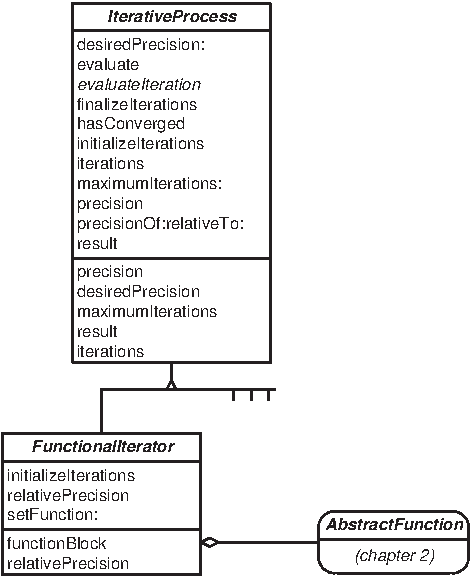
\includegraphics[width=6cm]{Figures/IterationClasses}
\caption{Class diagram for iterative process
classes}\label{cl:iteration}
\end{figure}
This chapter first discusses the implementation of a
general-purpose iterative process. Then, we describe a
generalization for the finding of a numerical result. Other
chapters discuss examples of sub-classing of these classes to
implement specific algorithms.

Iteration is used to find the solution of a wide variety of
problems other than just function evaluation. Finding the location
where a function is zero, reached a maximum or a minimum is
another example. Some data mining algorithms also use iteration to
find a solution (\cf section \ref{sec:cluster}).

\section{Successive approximations}
\label{sec:iteration} A general-purpose iterative process can be
decomposed in three main steps:
\begin{itemize}
  \item a set-up phase
  \item an iteration phase until the result is acceptable
  \item a clean-up phase
\end{itemize}
\noindent These steps are translated schematically into the flow
diagram shown in Figure \ref{fig:itercoarse}.
\begin{figure}
\centering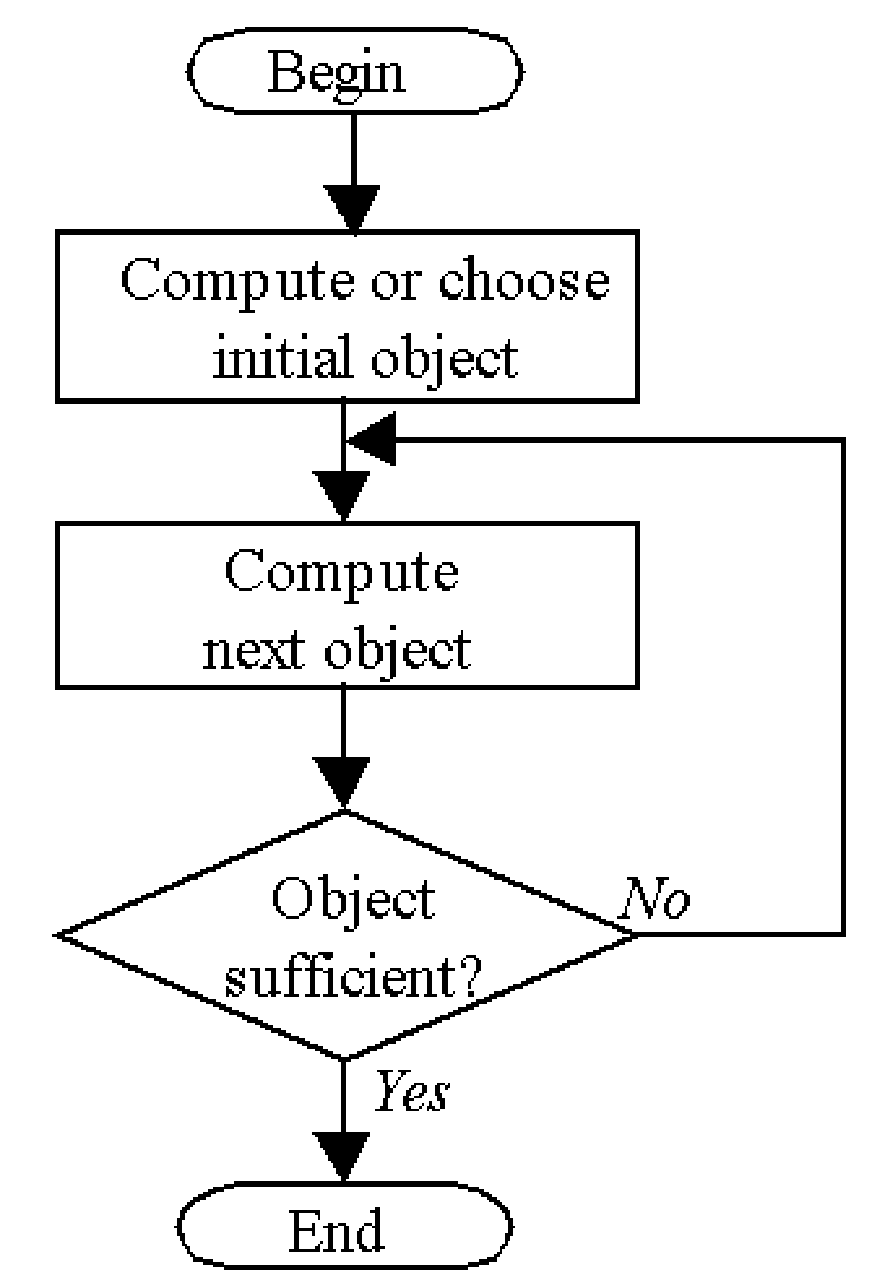
\includegraphics[width=5cm]{Figures/IterationCoarseFlow}
\caption{Successive approximation algorithm}\label{fig:itercoarse}
\end{figure}

The set-up phase allows determining constant parameters used by
the subsequent computations. Often a first estimation of the
solution is defined at this time. In any case an object
representing the approximate solution is constructed. Depending on
the complexity of the problem a class will explicitly represent
the solution object. Otherwise the solution shall be described by
a few instance variables of simple types (numbers and arrays).

After the set-up phase the iterative process proper is started. A
transformation is applied to the solution object to obtain a new
object. This process is repeated unless the solution object
resulting from the last transformation can be considered close
enough to the sought solution.

During the clean-up phase resources used by the iterative process
must be release. In some cases additional results may be derived
before leaving the algorithm.

\noindent Let us now explicit each of the three stages of the
algorithm.

The step computing or choosing an initial object is strongly
dependent on the nature of the problem to be solved. In some
methods, a good estimate of the solution can be computed from the
data. In others using randomly generated objects yields good
results. Finally, one can also ask the application's user for
directions. In many cases this step is also used to initialize
parameters needed by the algorithm.

The step computing the next object contains the essence of the
algorithm. In general a new object is generated based on the
history of the algorithm.

The step deciding whether or not an object is sufficiently close
to the sought solution is more general. If the algorithm is
capable of estimating the precision of the solution --- that is,
how close the current object is located from the exact solution
--- one can decide to stop the algorithm by comparing the
precision to a desired value. This is not always the case,
however. Some algorithms, genetic algorithms for example, do not
have a criterion for stopping.

Whether or not a well-defined stopping criterion exists, the
algorithm must be prevented from taking an arbitrary large amount
of time. Thus, the object implementing an iterative process ought
to keep track of the number of iterations and interrupt the
algorithm if the number of iterations becomes larger than a given
number.

\rubrique{Design}
%\marginpar{Figure \ref{cl:iteration} with the box {\bf IterativeProcess} grayed.}
Now we can add some details to the
algorithm. The new details are shown in figure \ref{fig:iterfine}.
\begin{figure}
\centering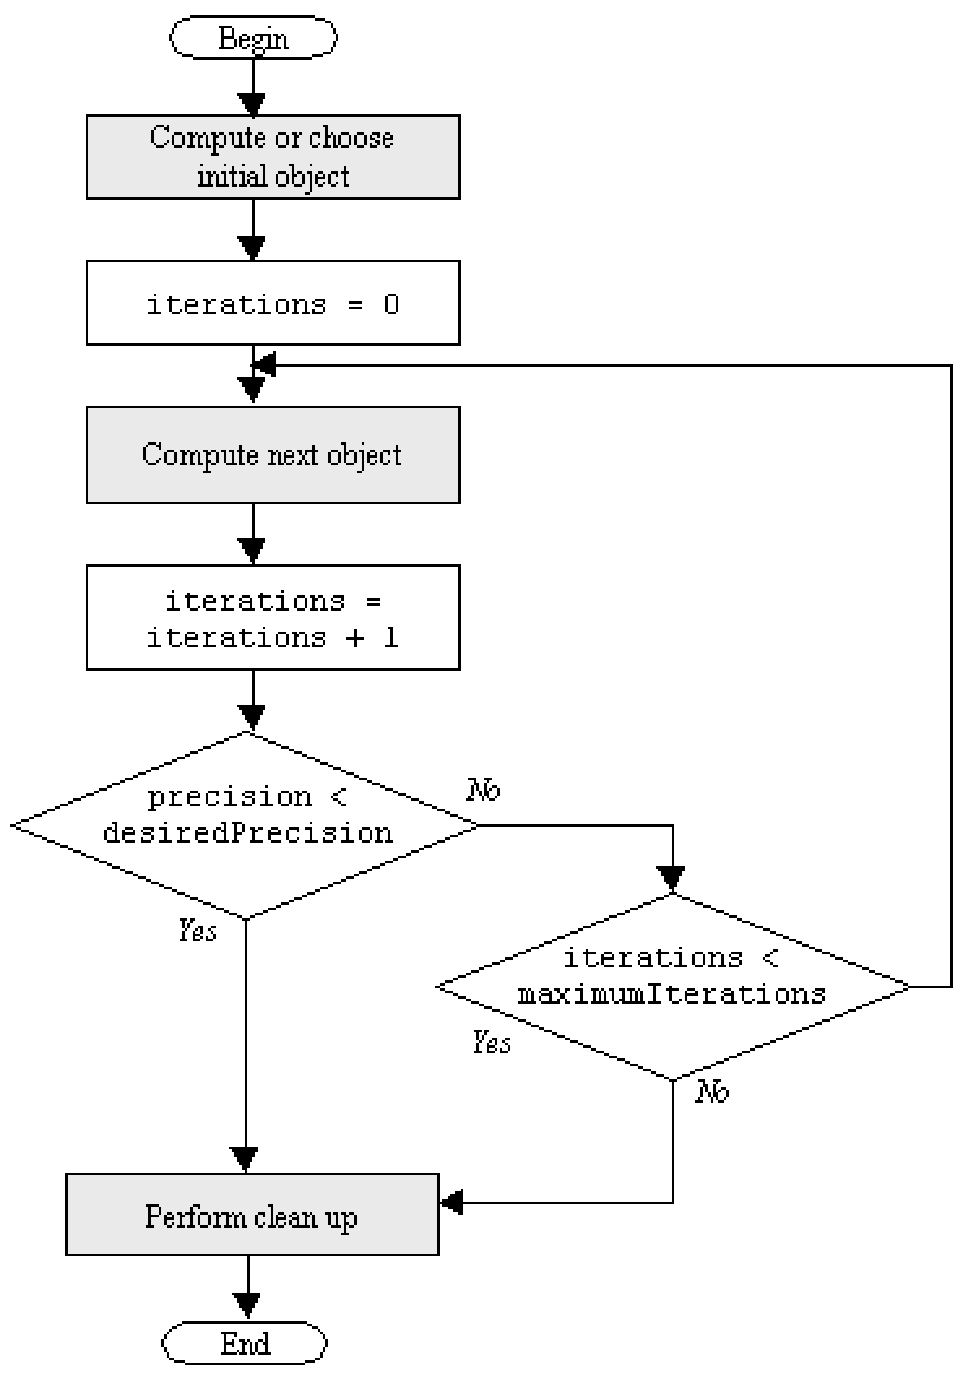
\includegraphics[width=4in]{Figures/IterationFineFlow}
\caption{Detailed algorithm for successive
approximations}\label{fig:iterfine}
\end{figure}
This schema allows us to determine the structure of a general
object implementing the iterative process. It will be implemented
as an abstract class. An abstract class is a class with does not
have object instances. A object implementing a specific algorithm
is an instance of a particular subclass of the abstract class.

The gray boxes in figure \ref{fig:iterfine} represent the methods,
which must be implemented explicitly by the subclass. The abstract
class calls them. However, the exact implementation of these
methods is not defined at this stage.
Such methods are called {\textsl hook} methods.

Using this architecture the abstract class is able to implement
the iterative process without any deep knowledge of the algorithm.
Algorithm specific methods are implemented by the subclass of the
abstract class.

Let us call \code{IterativeProcess} the class of the abstract
object. The class \code{IterativeProcess} needs the following
instance variables:
\begin{itemize}
\item \code{iterations}keeps track of the number of iterations, that is the number of successive
approximations,
\item \code{maximumIterations} maximum number of allowed iterations,
\item \code{desiredPrecision} the precision to attain, that is, how close to the solution should the solution object be when the algorithm is
terminated,
\item \code{precision} the precision achieved by the process. Its value is updated after each iteration and it is used to decide when to stop.
\end{itemize}
\begin{figure}
\centering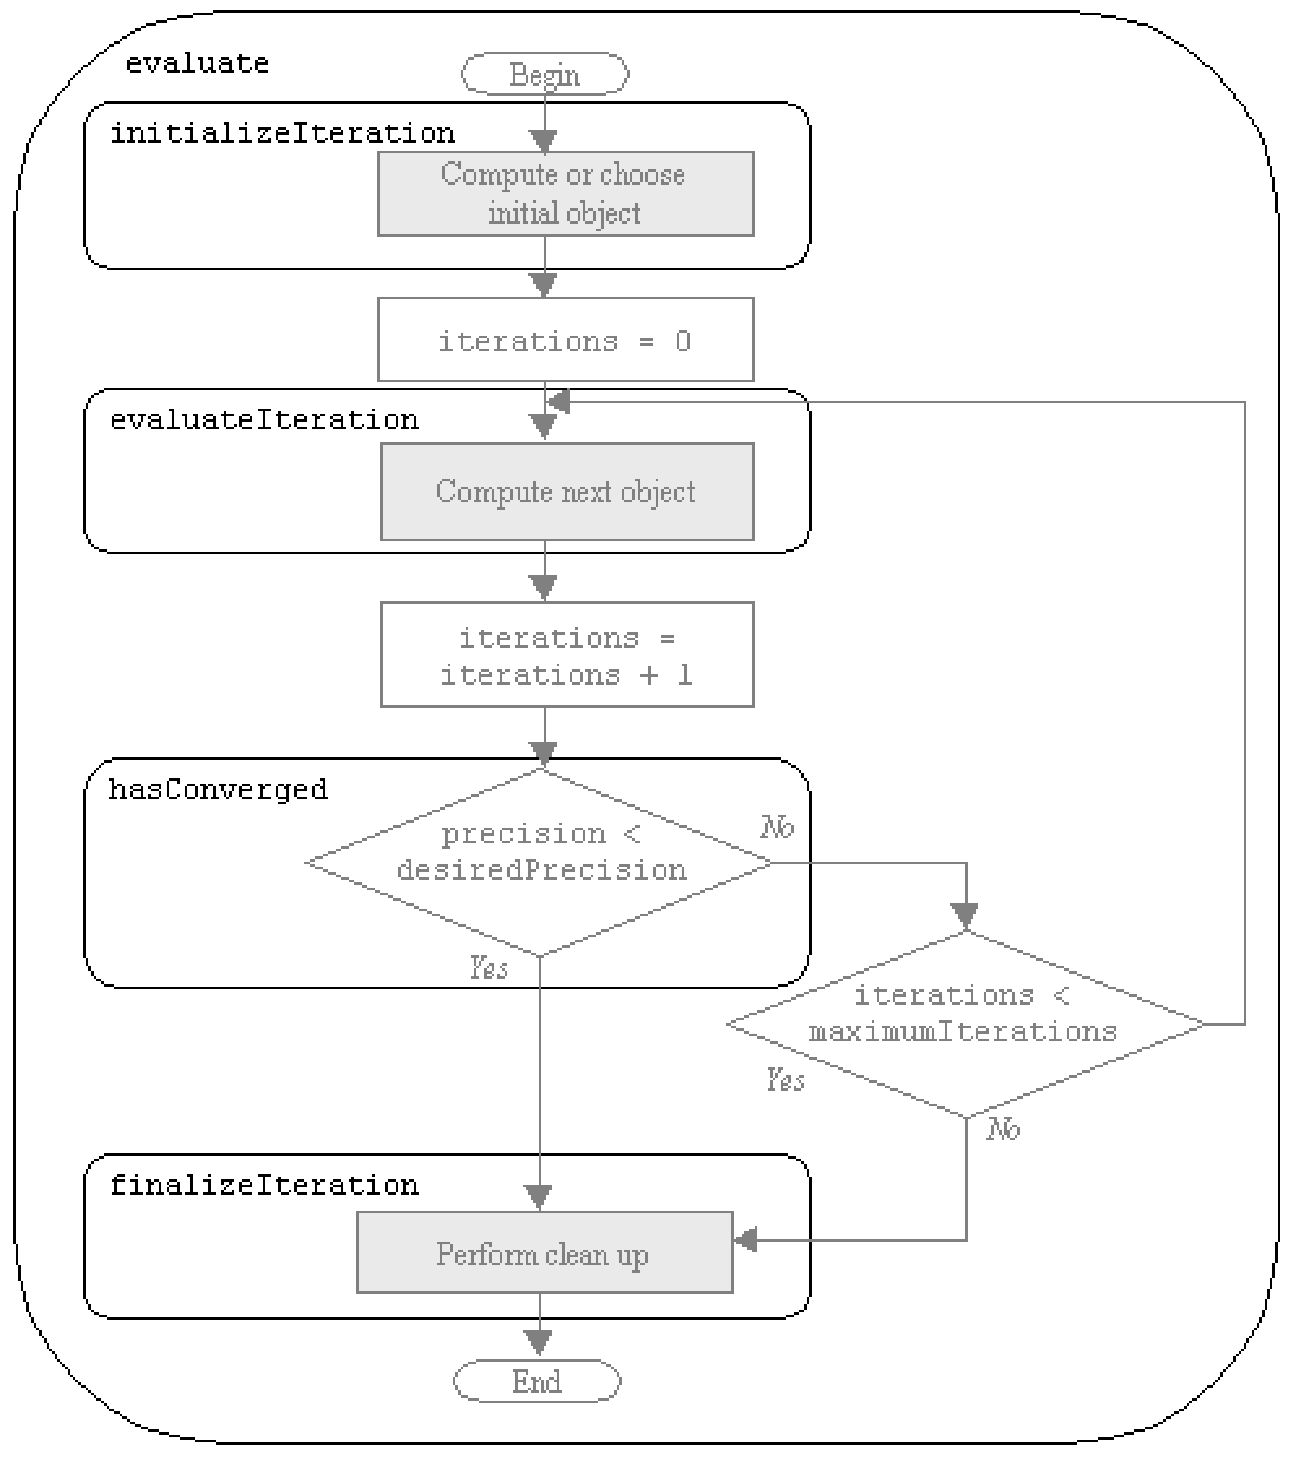
\includegraphics[width=4in]{Figures/IterationMethods}
\caption{Methods for successive
approximations}\label{fig:itermeth}
\end{figure}
The methods of the class \code{IterativeProcess} are shown in
figure \ref{fig:itermeth} in correspondence with the general
execution flow shown in figure \ref{fig:iterfine}. The two methods
\code{initializeIterations} and \code{finalizeIterations} should be
implemented by the subclass but the abstract class provides a
default behavior: doing nothing. The method \code{evaluateIteration} must be implemented by each subclass.

Since the precision of the last iteration is kept in an instance
variable, the method \code{hasConverged} can be called at any time
after evaluation, thus providing a way for client classes to check
whether the evaluation has converged or not.

\subsection{Iterative process --- Smalltalk implementation}
\label{sec:siteration}
Even though we are dealing for the moment
with an abstract class we are able to present a scenario of use
illustrating the public interface to the class. Here is how a
basic utilization of an iterative process object would look like.
\begin{displaycode}{Smalltalk}
| iterativeProcess result |
iterativeProcess := <a subclass of DhbIterativeProcess> new.
result := iterativeProcess evaluate.
iterativeProcess hasConverged
   ifFalse:[ <special case processing> ].
\end{displaycode}

The first statement creates an object to handle the iterative
process. The second one performs the process and retrieves the
result, whatever it is. The final statement checks for
convergence.

To give the user a possibility to have more control, one can
extend the public interface of the object to allow defining the
parameters of the iterative process: the desired precision and the
maximum number of iterations. In addition, the user may want to
know the precision of the attained result and the number of
iterations needed to obtain the result. The following code sample
shows an example of use for all public methods defined for an
iterative process. The precision of the attained result and the
number of iterations are printed on the transcript window.

\begin{displaycode}{Smalltalk}
| iterativeProcess result precision |
iterativeProcess := <a subclass of DhbIterativeProcess> new.
iterativeProcess desiredPrecision: 1.0e-6; maximumIterations: 25.
result := iterativeProcess evaluate.
iterativeProcess hasConverged
   ifTrue: [ Transcript nextPutAll: 'Result obtained after '.
             iterativeProcess iteration printOn: Transcript.
             Transcript nextPutAll: 'iterations. Attained precision is'.
             iterativeProcess precision printOn: Transcript.
             ]
    ifFalse:[ Transcript nextPutAll: 'Process did not converge'.].
Transcript cr.
\end{displaycode}

Listing \ref{lst:iteration} shows the Smalltalk implementation of the iterative process.

In the Smalltalk implementation, the class \code{IterativeProcess}
has one instance variable in addition to the ones described in the
preceding section. This variable, called \code{result}, is used to
keep the solution object of the process. The method \code{result}
allows direct access to it. Thus, all subclasses can use this
instance variable as a placeholder to store any type of result. As
a convenience the method \code{evaluate} also returns the instance
variable \code{result}.

Default values for the desired precision and the maximum number of
iterations are kept in class methods for easy editing. The method
initialize loads these default values for each newly created
instance. The default precision is set to the machine precision
discussed in section \ref{sec-rounding}.

The methods used to modify the desired precision (\code{desiredPrecision:}) and the maximum number of iterations (\code{maximumIterations:}) check the value to prevent illegal
definitions, which could prevent the algorithm from terminating.

Since there is no explicit declaration of abstract class and abstract methods in Smalltalk\footnote{An abstract class is a class containing at least an abstract method; an abstract method contains the single conventional statement: \code{self subclassResponsibility}} the three methods \code{initializeIterations}, \code{evaluateIteration} and \code{finalizeIterations}, are implemented with a reasonable default behavior.
The methods \code{initializeIterations} and \code{finalizeIterations} do nothing. The method \code{evaluateIteration} calls the method \code{subclassResponsibility}, which raises an
exception when called.
Using this technique is the Smalltalk way of creating an abstract method.
\begin{listing}[label=lst:iteration]{Smalltalk}
{Smalltalk implementation of an iterative process}
Object subclass: #PMIterativeProcess
   instanceVariableNames: 'precision desiredPrecision maximumIterations result iterations'
   classVariableNames: ''
   package: 'Math-Core-Process'
\end{listing}

\begin{displaycode}{Smalltalk}
PMIterativeProcess class >> defaultMaximumIterations
    ^50
\end{displaycode}

\begin{displaycode}{Smalltalk}
PMIterativeProcess class >> defaultPrecision
    ^PMFloatingPointMachine new defaultNumericalPrecision
\end{displaycode}

\begin{displaycode}{Smalltalk}
PMIterativeProcess >> desiredPrecision: aNumber
    aNumber > 0
        ifFalse: [ ^self error: 'Illegal precision: ', aNumber 
                                                         printString].
    desiredPrecision := aNumber.
\end{displaycode}

\begin{displaycode}{Smalltalk}
PMIterativeProcess >> evaluate
    iterations := 0.
    self initializeIterations.
    [iterations := iterations + 1.
    precision := self evaluateIteration.
    self hasConverged or: [iterations >= maximumIterations]] 
            whileFalse: [].
    self finalizeIterations.
    ^self result
\end{displaycode}

\begin{displaycode}{Smalltalk}
PMIterativeProcess >> evaluateIteration
    ^self subclassResponsibility
\end{displaycode}

\begin{displaycode}{Smalltalk}
PMIterativeProcess >> finalizeIterations
   "Perform cleanup operation if needed (must be implemented by subclass)."
\end{displaycode}

\begin{displaycode}{Smalltalk}
PMIterativeProcess >> hasConverged
    ^precision <= desiredPrecision
\end{displaycode}

\begin{displaycode}{Smalltalk}
PMIterativeProcess >> initialize
    desiredPrecision := self class defaultPrecision.
    maximumIterations := self class defaultMaximumIterations.
    ^self
\end{displaycode}

\begin{displaycode}{Smalltalk}
PMIterativeProcess >> initializeIterations
   "Initialize the iterations (must be implemented by subclass when needed)."
\end{displaycode}

\begin{displaycode}{Smalltalk}
PMIterativeProcess >> iterations
    ^iterations
\end{displaycode}

\begin{displaycode}{Smalltalk}
PMIterativeProcess >> maximumIterations: anInteger
    ( anInteger isInteger and: [ anInteger > 1])
        ifFalse: [ ^self error: 'Invalid maximum number of iteration: 
                                            ', anInteger printString].
    maximumIterations := anInteger
\end{displaycode}

\begin{displaycode}{Smalltalk}
PMIterativeProcess >> precision
    ^precision
\end{displaycode}

\begin{displaycode}{Smalltalk}
PMIterativeProcess >> precisionOf: aNumber1 relativeTo: aNumber2
    ^aNumber2 > PMFloatingPointMachine new defaultNumericalPrecision
        ifTrue: [ aNumber1 / aNumber2]
        ifFalse:[ aNumber1]
\end{displaycode}

\begin{displaycode}{Smalltalk}
PMIterativeProcess >> result
   ^result
\end{displaycode}

\begin{quote}
{\textbf Note:} The method \code{precisionOf:relativeTo:} implements
the computation of the relative precision. This is discussed in
section \ref{sec:siterrel}.
\end{quote}


\section{Evaluation with relative precision}
\label{sec:iterrel}
%\marginpar{Figure \ref{cl:iteration} with the box {\bf FunctionalIterator} grayed.}
So far we have made no
assumption about the nature of the solution searched by an
iterative process. In this section we want to discuss the case
when the solution is a numerical value.

As discussed in section \ref{sec-rounding} a floating-point number
is a representation with constant relative precision. It is thus
meaningless to use absolute precision to determine the convergence
of an algorithm. The precision of an algorithm resulting in a
numerical value ought to be determined relatively.

One way to do it is to have the method \code{evaluateIteration}
returning a relative precision instead of an absolute number.
Relative precision, however, can only be evaluated if the final
result is different from zero. If the result is zero, the only
possibility is to check for absolute precision. Of course, in
practice one does not check for equality with zero. The
computation of a relative precision is carried only if the
absolute value of the result is larger than the desired precision.

The reasoning behind the computation of the relative error is
quite general. Thus, a general-purpose class \code{FunctionalIterator} has been created to implement a method
computing the relative precision from an absolute precision and a
numerical result. In addition, since all subclasses of \code{FunctionalIterator} use a function a general method to handle the
definition of that function is also supplied.

\subsection{Relative precision --- Smalltalk  implementation}
\label{sec:siterrel} In this case the public interface is extended
with a creation method taking as argument the function on which
the process operates.
The code example of section \ref{sec:siteration} then becomes:
\begin{displaycode}{Smalltalk}
| iterativeProcess result |
iterativeProcess := <a subclass of PMFunctionalIterator>
                  function: ( PMPolynomial coefficients: #(1 2 3)).
result := iterativeProcess evaluate.
iterativeProcess hasConverged ifFalse:[ <special case processing>].
\end{displaycode}
In this example the function on which the process will operate is
the polynomial $3x^2+2x+1$ (\cf section \ref{sec:polynomial}).

Listing \ref{ls:iterrel} shows the implementation of the abstract
class \code{PMFunctionalIterator} in Smalltalk.

This class has one instance variable \code{functionBlock} to store
the function. A single class method allows creating a new instance
while defining the function.

As we have seen in section \ref{sec:stFunction}, a function can be
any object responding to the message value:. This allows supplying
any block of Smalltalk code as argument to the constructor method.
However, the user can also supply a class implementing the
computation of the function with a method with selector \code{value:}. For example, an instance of the class \code{PMPolynomial}
discussed in section \ref{sec:stPolynomial} can be used.

The instance method \code{setFunction:} is used to set the instance
variable \code{functionBlock}. In order to prevent a client class
from sending the wrong object, the method first checks whether the
supplied object responds to the message \code{value:}. This is one
way of ensuring that the arguments passed to a method conform to
the expected protocol. This way of doing is only shown as an
example, however. It is not recommend in practice. The
responsibility of supplying the correct arguments to a Smalltalk
method is usually the responsibility of the client class.

The method \code{initializeIterations} first checks whether a
function block has been defined. Then it calls the method \code{computeInitialValues}. This method is a hook method, which a
subclass must implement to compute the value of the result at the
beginning of the iterative process.

The computation of relative precision is implemented at two
levels. One general method, \code{precisionOf:relativeTo:},
implemented by the superclass allows the computation of the
relative precision relative to any value. Any iterative process
can use this method. The method \code{relativePrecision} implements
the computation of the precision relative to the current result.

\begin{listing}[label=lst:iterrel]{Smalltalk}
{Smalltalk implementation of the class PMFunctionalIterator}
PMIterativeProcess subclass: #PMFunctionalIterator
   instanceVariableNames: 'functionBlock'
   classVariableNames: ''
   package: 'Math-DHB-Numerical-Math-FunctionIterator'
\end{listing}

\begin{displaycode}{Smalltalk}
PMFunctionalIterator class >> function: aBlock
    ^self new setFunction: aBlock; yourself
\end{displaycode}

\begin{displaycode}{Smalltalk}
PMFunctionalIterator >> initializeIterations
    functionBlock isNil ifTrue: [self error: 'No function supplied'].
    self computeInitialValues
\end{displaycode}

\begin{displaycode}{Smalltalk}
PMFunctionalIterator >> relativePrecision: aNumber
    ^self precisionOf: aNumber relativeTo: result abs
\end{displaycode}

\begin{displaycode}{Smalltalk}
PMFunctionalIterator >> setFunction: aBlock
    ( aBlock respondsTo: #value:)
        ifFalse:[ self error: 'Function block must implement the 
                                                      method value:'].
    functionBlock := aBlock
\end{displaycode}

\section{Examples}
As we have dealt with abstract classes, this chapter did not give
concrete examples of use. By consulting the rest of this book the
reader will find numerous examples of subclasses of the two
classes described in this chapter. Table \ref{tb:iteration} lists
the sections where each algorithm using the iterative process
framework is discussed.
\begin{table}[h]
  \centering
  \caption{Algorithms using iterative processes}\label{tb:iteration}
\vspace{1 ex}
\begin{tabular}{|l|l|c|} \hline
\textbf{Algorithm or class of algorithm}&\textbf{Superclass}&\textbf{
Chapter or section}
\\ \hline Zero finding&Function iterator&Chapter \ref{ch:zeroes}
\\ \hline Integration&Function iterator&Chapter
\ref{ch:integration}
\\ \hline Infinite series and continued fractions&Function
iterator&Chapter \ref{ch:series}  \\ \hline Matrix
eigenvalues&Iterative process&Section \ref{sec:eigen}
\\ \hline Non-linear least square fit&Iterative process&Section
\ref{sec:lsfnonlin}
\\ \hline Maximum likelihood fit&Iterative process&Section \ref{sec:mlfhist} \\
\hline Function minimization&Function iterator&Chapter
\ref{ch:minimization}  \\ \hline Cluster analysis&Iterative
process&Section \ref{sec:cluster} \\ \hline
\end{tabular}

\end{table}

%\ifx\wholebook\relax\else\end{document}\fi

%\ifx\wholebook\relax\else
%\documentclass[twoside]{book}
%\usepackage[active]{srcltx}
%\usepackage[LY1]{fontenc}
%\usepackage{url}
\makeatletter
\def\url@leostyle{%
  \@ifundefined{selectfont}{\def\UrlFont{\sf}}{\def\UrlFont{\sffamily}}}
\makeatother
% Now actually use the newly defined style.
\urlstyle{leo}

\usepackage{graphicx}
\def\etc{{\textit{etc}}}
\def\eg{{\textit{e.g.}}}
\def\ie{{\textit{i.e.}}}
\def\cf{{\textit{c.f.}}\ }
\def\erf{\mathop{\textrm{erf}}}
\def\sign{\mathop{\textrm{sign}}}
\def\prob{\mathop{\textrm{Prob}}}
\def\var{\mathop{\textrm{var}}}
\def\mod{\mathop{\textrm{mod}}}
\def\cor{\mathop{\textrm{cor}}}
\def\cov{\mathop{\textrm{cov}}}
\def\cl{\mathop{\textrm{CL}}}
\def\kg{\mathop{\textrm{Kg}}}
\def\patstyle#1{{\textsc #1}}
\def\th{^{\mathop{\textrm{th}}}}
%\def\st#1{^{\mathop{\rm #1}}}
\def\note#1{\begin{quote}{\textbf{Note:}} #1\end{quote}}
\def\braket#1{\left\langle #1\right\rangle}
\def\order#1{\let\o=#1$\mathcal{O}$\ifx\o 1$\left(n\right)$\else$\left(n^{#1}\right)$\fi}
%\newtheorem{privListing}{Listing}[chapter]
%\newenvironment{listing}{\vskip 3ex\hrule\vskip 1ex\begin{privListing}}{\end{privListing}\hrule\vskip 1ex}
\newtheorem{privExample}{Code example}[chapter]
\newenvironment{codeExample}{\begin{privExample}\begin{quote}\tt}{\end{quote}\end{privExample}}
\def\relboxl#1#2{\hbox to #1\hsize{#2\hfil}}
\def\relboxc#1#2{\hbox to #1\hsize{\hfil #2\hfil}}
\def\relboxr#1#2{\hbox to #1\hsize{\hfil #2}}
\def\transpose#1{\textbf{#1}^{\mathop\textrm{T}}}
\def\inverse#1{\textbf{#1}^{-1}}
%\def\tm{$^{\mathop{\rm TM}}$}
\def\tm{ }
\newenvironment{mainEquation}{\marginpar[\vspace{3 ex} Main
equation$\Rightarrow$]{\vspace{3 ex}$\Leftarrow$Main
equation}\begin{equation}}{\end{equation}}
\def\rubrique#1{\paragraph{#1}\hfil\par\noindent}

%\begin{document}
%\fi

\chapter{Finding the zero of a function}
\label{ch:zeroes} \vspace{1 ex}
\begin{flushright} {\textsl Le z\'ero, collier du n\'eant.}\footnote{The zero, a necklace for emptiness.}\\ Jean Cocteau
\end{flushright}
\vspace{1 ex}
The zeroes of a function are the values of the
function's variable for which the value of the function is zero.
Mathematically, given the function $f\left(x\right)$, $z$ is a
zero of when $f\left(z\right)=0$. This kind of problem is can be
extended to the general problem of computing the value of the
inverse function, that is finding a value $x$ such that
$f\left(x\right)=c$ where $c$ is a given number. The inverse
function is noted as $f^{-1}\left(x\right)$. Thus, one wants to
find the value of $f^{-1}\left(c\right)$ for any $c$. The problem
can be transformed into the problem of finding the zero of the
function $\tilde{f}\left(x\right)=f\left(x\right)-c$.

The problem of finding the values at which a function takes a
maximum or minimum value is called searching for the extremes of a
function. This problem can be transformed into a zero-finding
problem if the derivative of the function can be easily computed.
The extremes are the zeroes of the function's derivative.

\noindent Figure \ref{cl:zeroFinding} shows the class diagram of
the classes discussed in this chapter.
\begin{figure}
\centering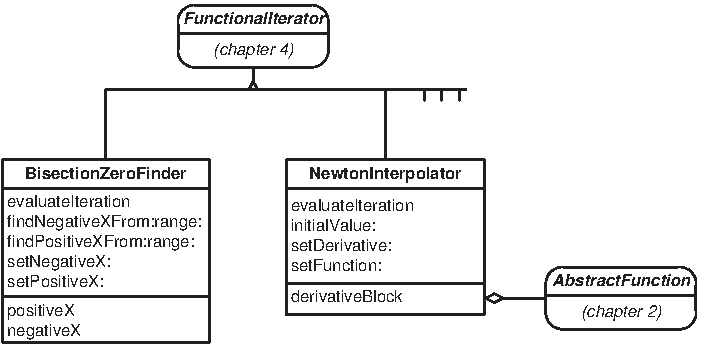
\includegraphics[width=10cm]{Figures/ZeroClassDiagram}
\caption{Class diagram for zero finding
classes}\label{cl:zeroFinding}
\end{figure}


\section{Introduction}
Let us begin with a concrete example.

Often an experimental result is obtained by measuring the same
quantity several times. In scientific publications, such a result
is published with two numbers: the average and the standard
deviation of the measurements. This is true for medical
publication as well. As we have already discussed in section
\ref{sec:errorFunctionDef}, obstetricians prefer to think in terms
of risk and prefer to use centiles instead of average and standard
deviation. Assuming that the measurements were distributed
according to a normal distribution (\cf section
\ref{sec:normdist}), the 90th centile is the solution to the
following equation:
\begin{equation}
\label{eq:centile90}
  \erf\left(x\right)=0.9
\end{equation}
That is, we need to find the zero of the function
$f\left(x\right)=\erf\left(x\right)-0.9$. The answer is $x=1.28$
with a precision of two decimals. Thus, if $\mu$ and $\sigma$ are
respectively the average and standard deviation of a published
measurement, the 90th centile is given by $\mu+1.28\cdot\sigma$.
Using equation \ref{eq:erfneg} the 10th centile is given by
$\mu-1.28\cdot\sigma$.

\section{Finding the zeroes of a function --- Bisection method}
\label{sec:bisection}
%\marginpar{Figure \ref{cl:zeroFinding} with the box {\textbf BisectionZeroFinder} grayed.}
Let assume that one knows two values of $x$ for which the function takes values of
opposite sign. Let us call $x_{pos}$ the value such
that $f\left(x_{pos}\right)>0$ and $x_{neg}$ the value such that $f\left(x_{neg}\right)<0$.
If the function is continuous between $x_{pos}$ and
$x_{neg}$, there exists at least one zero of the
function in the interval $\left[ x_{pos},x_{neg}\right]$. This is illustrated in figure
\ref{fig:bisection}. If the function $f$ is not continuous over
the interval where the sign of the function changes, then the
presence of a zero cannot be guaranteed\footnote{The inverse
function is such an example. It changes sign over 0 but has no
zeroes for any finite $x$}. The continuity requirement is
essential for the application of the bisection algorithm.

The values $x_{pos}$ and $x_{neg}$ are
the initial values of the bisection algorithm. The algorithm goes
as follows:
\begin{enumerate}
  \item Compute $x={x_{pos}-x_{neg}\over2}$.
  \item If $f\left(x\right)>0$, set $x_{pos}=x$ and
  goto step 4.
  \item Otherwise set $x_{neg}=x$.
  \item If $\left|x_{pos},x_{neg}\right|>\epsilon$ go back
to step 1. $\epsilon$ is the desired precision of the solution.
\end{enumerate}
The first couple of steps of the bisection algorithm are
represented geometrically on figure \ref{fig:bisection}. Given the
two initial values, $x_{pos}$ and $x_{neg}$, the first iteration of the algorithm replaces $x_{pos}$ with $x_1$. The next step replaces $x_{neg}$ with $x_2$.
\begin{figure}
\centering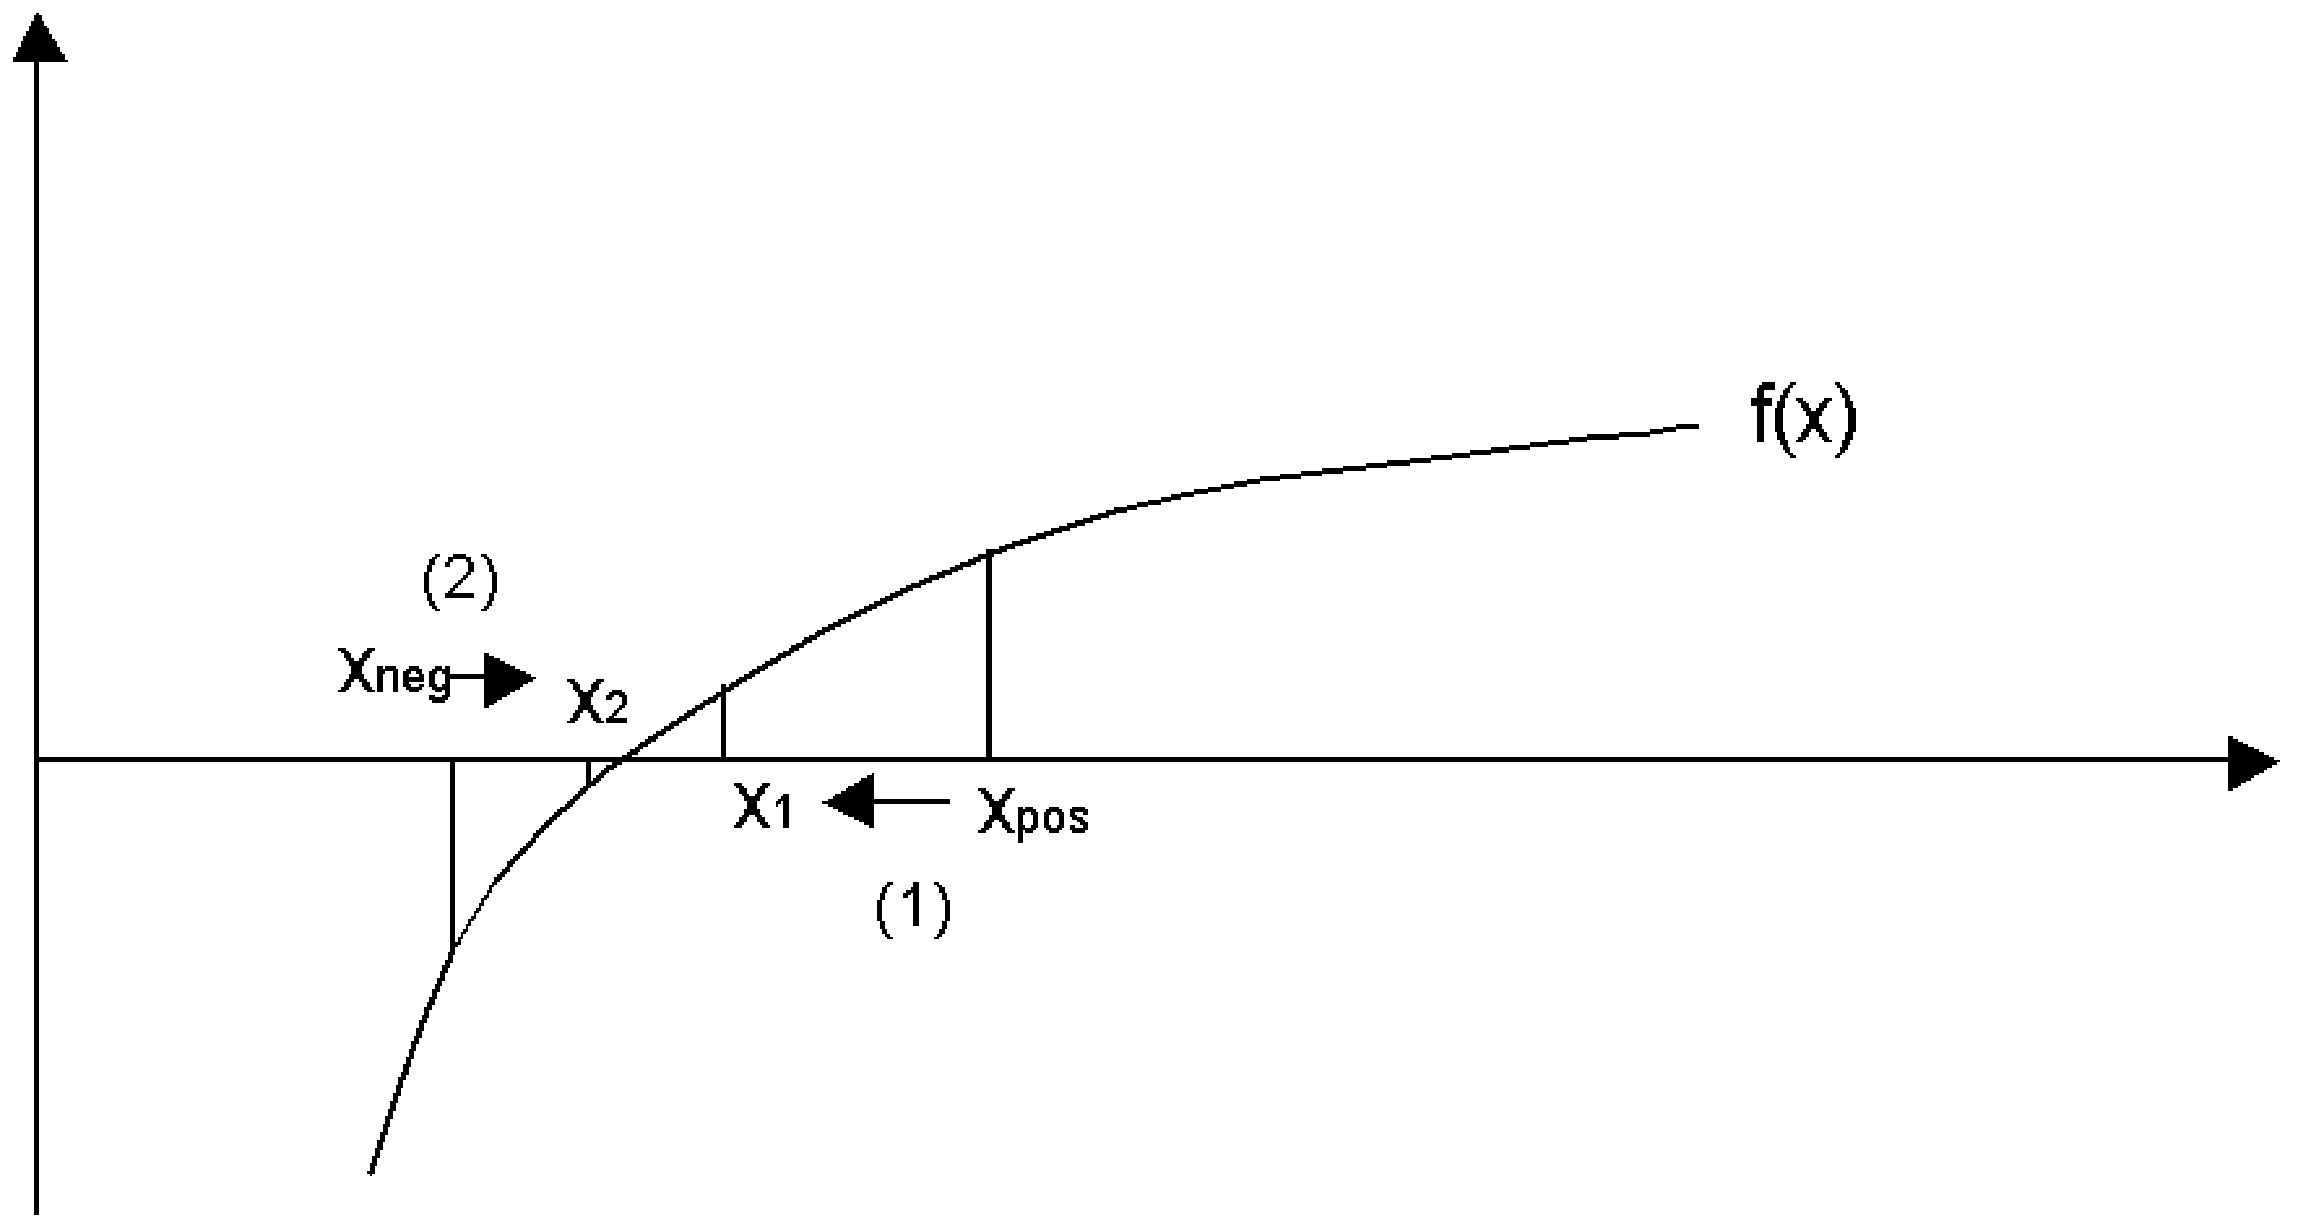
\includegraphics[width=12cm]{Figures/BissectionGraph}
\caption{The bisection algorithm}\label{fig:bisection}
\end{figure}

For a given pair of initial values, $x_{pos}$ and $x_{neg}$, the number of iterations required to attain a precision $\epsilon$ is given by:
\begin{equation}
\label{eq:bissectime}
  n=\left\lceil\log_2{\displaystyle\left| x_{pos},x_{neg}\right| \over
\displaystyle\epsilon}\right\rceil.
\end{equation}
For example if the distance between the two initial values is 1
the number of iterations required to attain a precision of
$10^{-8}$ is 30. It shows that the bisection algorithm is rather
slow.

Knowledge of the initial values, $x_{pos}$ and $x_{neg}$, is essential for starting the algorithm.
Methods to define them must be supplied. Two convenience methods
are supplied to sample the function randomly over a given range to
find each initial value. The random number generator is discussed
in section \ref{sec:random}.

The bisection algorithm is a concrete implementation of an
iterative process. In this case, the method \code{evaluateIteration} of figure \ref{fig:itermeth} implements steps
2, 3 and 4. The precision at each iteration is $\left|
x_{pos}-x_{neg}\right|$ since the zero
of the function is always inside the interval defined by
$x_{pos}$ and $x_{neg}$.

\subsection{Bisection algorithm --- General  implementation}

The class of the object implementing the bisection algorithm is a
subclass of the abstract class \code{FunctionalIterator}.
The class \code{BisectionZeroFinder} needs the following additional instance variables.
\begin{description}
  \item[\texttt positiveX]$x_{pos}$ and
  \item [\texttt negativeX]$x_{neg}$
\end{description}
The bisection algorithm proper is implemented only within the
method \code{evaluateIteration}.
Other necessary methods have already been implemented in the iterative process class.

\subsection{Bisection algorithm --- Smalltalk  implementation}
Finding the zero of a function is performed by creating an
instance of the class \code{PMBisectionZeroFinder} and giving the
function as the argument of the creation method as explained in
section \ref{sec:siterrel}. For example the following code finds
the solution of equation \ref{eq:centile90}.
\begin{displaycode}{Smalltalk}
| zeroFinder result |
zeroFinder:= PMBisectionZeroFinder function: [ :x | x errorFunction - 0.9].
zeroFinder setPositiveX: 10; setNegativeX: 0.
result := zeroFinder evaluate. zeroFinder
hasConverged
   ifFalse:[ <special case processing>].
\end{displaycode}
The second line creates the object responsible to find the zero.
The third line defines the initial values, $x_{pos}$ and $x_{neg}$.
The fourth line performs the algorithm and stores the result if the algorithm has converged.
The last two lines check for convergence and take corrective action if the algorithm did not converge.

Listing \ref{ls:bisection} shows the implementation of the bisection zero finding algorithm in Smalltalk.

The class \code{PMBisectionZeroFinder} is a subclass of the class \code{PMFunctionalIterator}. As one can see only a few methods need to be implemented.
Most of them pertain to the definition of the initial interval.
In particular, convenience methods are supplied to find a positive and negative function value over a given interval.

The methods defining the initial values, $x_{pos}$ and $x_{neg}$, are \code{setPositiveX:} and \code{setNegativeX:} respectively.
An error is generated in each method if the function's value does not have the proper sign.
The convenience methods to find random starting values are respectively \code{findPositiveXFrom:range:} and \code{findNegativeXFrom:range:}.
The method \code{computeInitialValues} does not compute the initial values. Instead it makes sure that $x_{pos}$ and $x_{neg}$ have been properly defined.

\begin{listing} Smalltalk implementation of the bisection algorithm \label{ls:bisection}
$$\halign{ #\hfil&\quad#\hfil\cr {\sl Class}& {\Large\bf DhbBisectionZeroFinder}\cr
{\sl Subclass of }&{\tt DhbFunctionalIterator}\cr\noalign{\vskip 1ex}

{\sl Instance variable names:}&\parbox[t]{4 in}{\tt  positiveX negativeX }\cr\noalign{\vskip 1ex}}$$


Instance methods
{\parskip 1ex\par\noindent}
{\bf computeInitialValues}
\begin{verbatim}
    positiveX isNil
        ifTrue: [ self error: 'No positive value supplied'].
    negativeX isNil
        ifTrue: [ self error: 'No negative value supplied'].

\end{verbatim}
{\bf evaluateIteration}
\begin{verbatim}
    result := ( positiveX + negativeX) * 0.5.
    ( functionBlock value: result) > 0
        ifTrue: [ positiveX := result]
        ifFalse:[ negativeX := result].
    ^self relativePrecision: ( positiveX - negativeX) abs

\end{verbatim}
{\bf findNegativeXFrom:} {\tt aNumber1} {\bf range:} {\tt aNumber2}
\begin{verbatim}
    | n |
    n := 0.
    [ negativeX := Number random * aNumber2 + aNumber1.
      ( functionBlock value: negativeX) < 0
        ] whileFalse: [ n := n + 0.1.
                        n > maximumIterations
                            ifTrue: [ self error: 'Unable to find a 
                                            negative function value'].
                      ].

\end{verbatim}
{\bf findPositiveXFrom:} {\tt aNumber1} {\bf range:} {\tt aNumber2}
\begin{verbatim}
    | n |
    n := 0.
    [ positiveX := Number random * aNumber2 + aNumber1.
      ( functionBlock value: positiveX) > 0
        ] whileFalse: [ n := n + 1.
                        n > maximumIterations
                            ifTrue: [ self error: 'Unable to find a 
                                            positive function value'].
                      ].

\end{verbatim}
{\bf setNegativeX:} {\tt aNumber}
\begin{verbatim}
    ( functionBlock value: aNumber) < 0
        ifFalse:[ self error: 'Function is not negative at x = ', 
                                                 aNumber printString].
    negativeX := aNumber.

\end{verbatim}
{\bf setPositiveX:} {\tt aNumber}
\begin{verbatim}
    ( functionBlock value: aNumber) > 0
        ifFalse:[ self error: 'Function is not positive at x = ', 
                                                 aNumber printString].
    positiveX := aNumber.

\end{verbatim}


\end{listing}

\section{Finding the zero of a function --- Newton's method}
\label{sec:newton}
%\marginpar{Figure \ref{cl:zeroFinding} with the box {\bf NewtonZeroFinder} grayed.}
Isaac Newton has designed an algorithm working by successive approximations\cite{Bass}.
Given a value $x_0$ chosen in the vicinity of the desired zero, the following series:
\begin{mainEquation}
\label{eq:newtonZero}
  x_{n+1}=x_n-{f\left(x_n\right)\over f^{\prime}\left(x_n\right)},
\end{mainEquation}
where $f^{\prime}\left(x\right)$ is the first derivative of $f\left(x\right)$, converges toward a zero of the function.
This algorithm is sometimes called Newton-Ralphson\cite{Press}.

Figure \ref{fig:newtonZero} shows the geometrical interpretation
of the series. $f^{\prime}\left(x\right)$ is the slope of the
tangent to the curve of the function $f\left(x\right)$ at the
point $x_n$. The equation of this tangent is thus given by:
\begin{figure}
\centering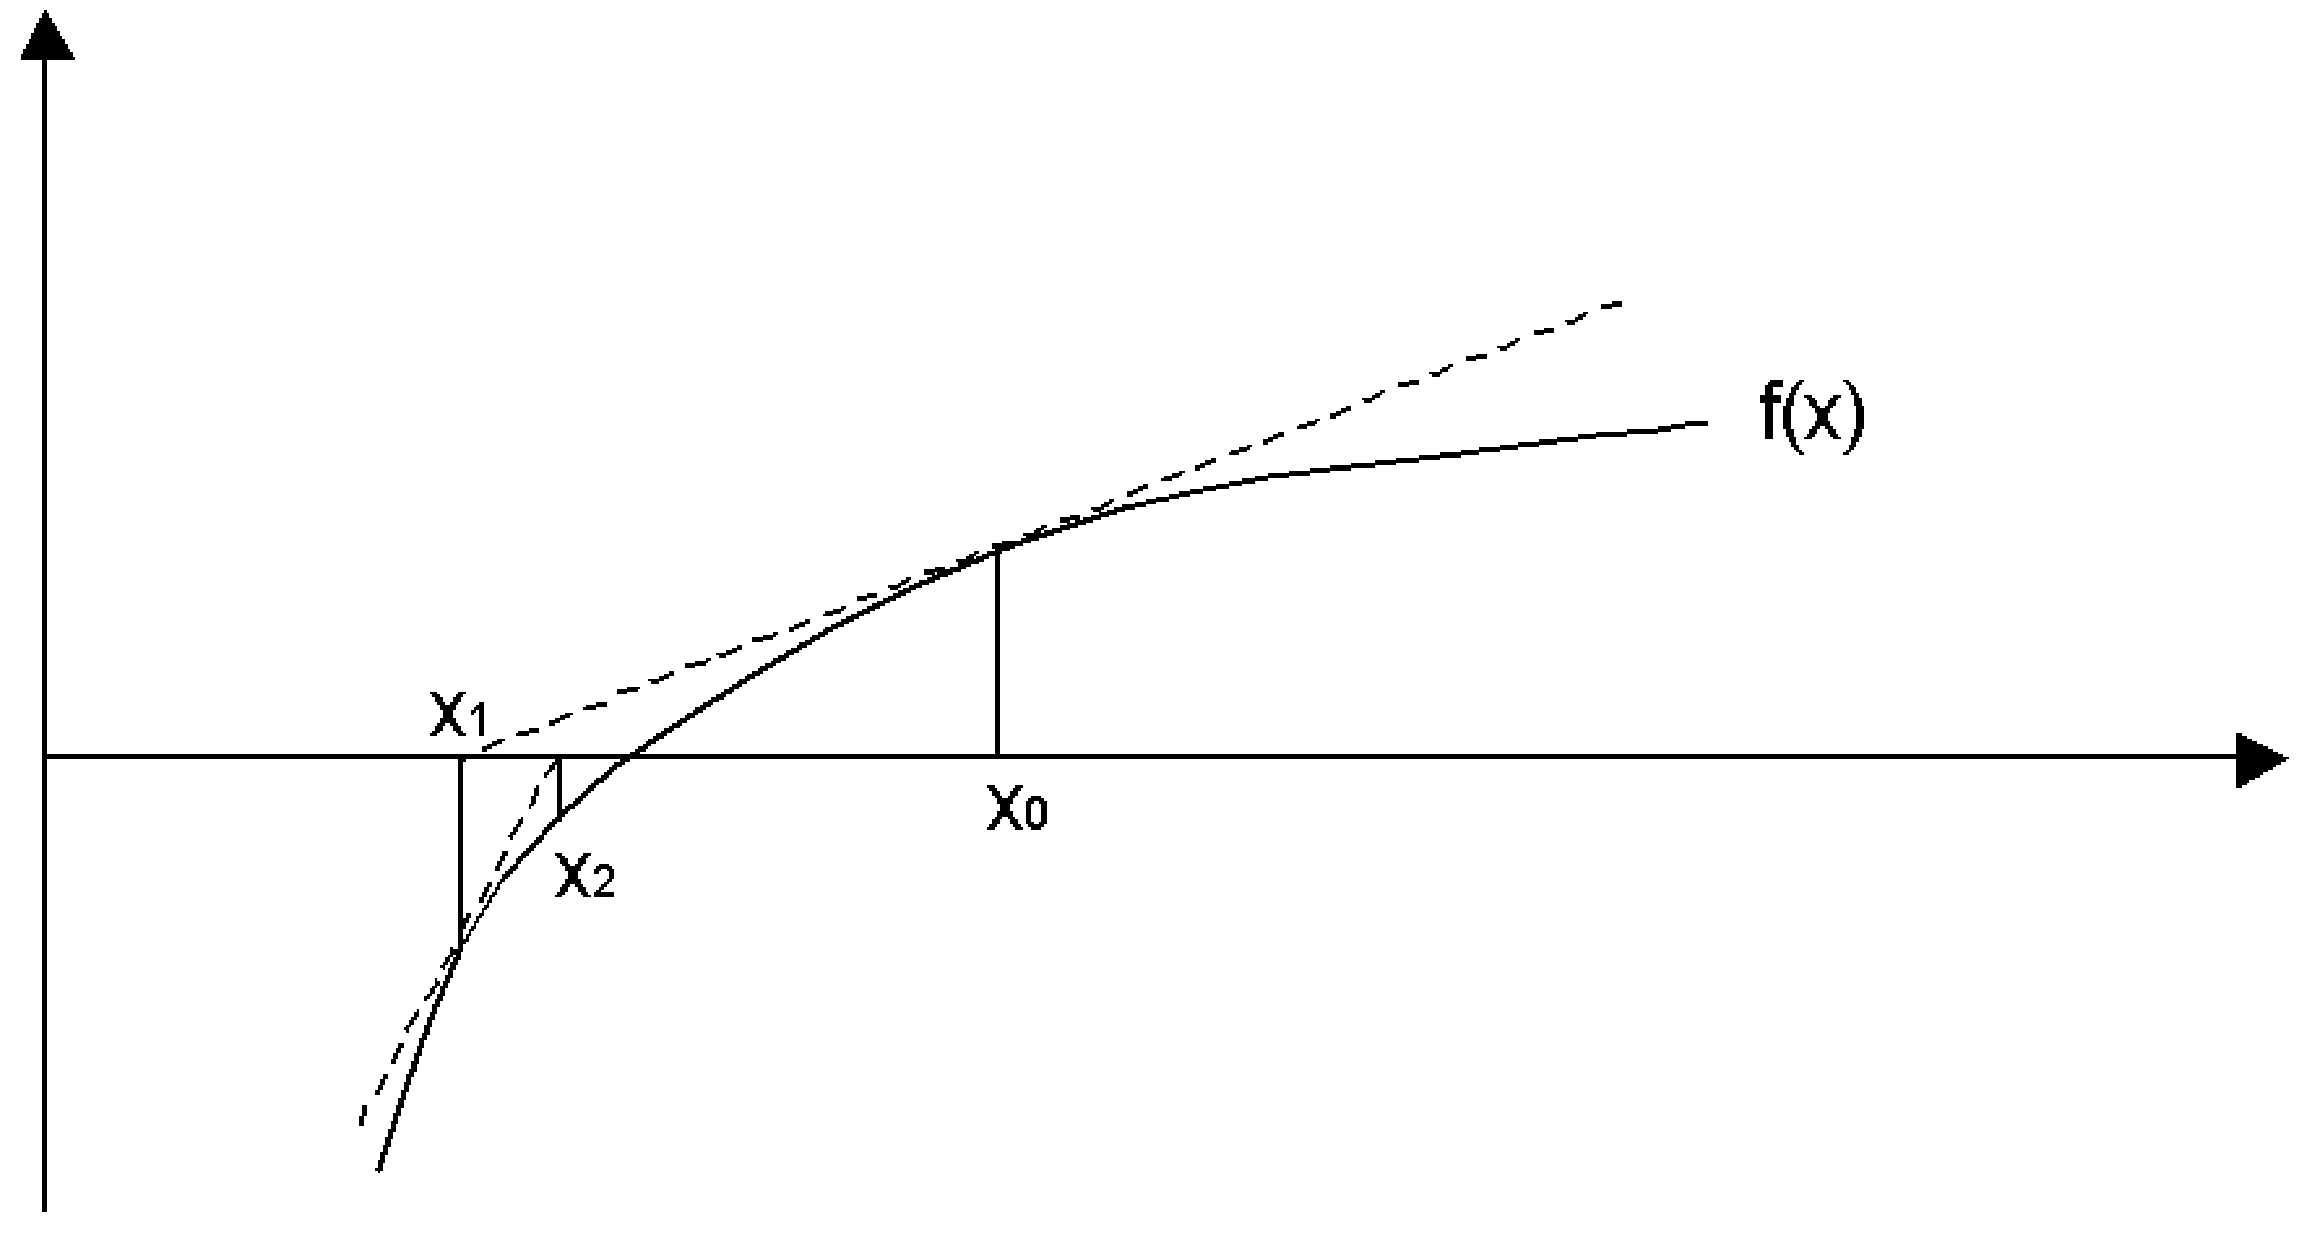
\includegraphics[width=12cm]{Figures/NewtonGraph}
\caption{Geometrical representation of Newton's zero finding
algorithm}\label{fig:newtonZero}
\end{figure}
\begin{equation}
  y=\left(x-x_n\right)\cdot f^{\prime}\left(x_n\right)+f\left(x_n\right)
\end{equation}
One can then see that $x_{n+1}$ is the point where the tangent to
the curve at the point $x_n$ crosses the $x$-axis. The algorithm
can be started at any point where the function's derivative is
non- zero.

The technique used in Newton's algorithm is a general technique
often used in approximations. The function is replaced by a linear
approximation\footnote{Mathematically, this corresponds to
estimate the function using the first two terms of its Taylor
series.}, that is a straight line going through the point defined
by the preceding value and its function's value. The slope of the
straight line is given by the first derivative of the function.
The procedure is repeated until the variation between the new
value and the preceding one is sufficiently small.
We shall see other examples of this technique in the remainder of this book
(\cf sections \ref{sec:lsfnonlin}, \ref{sec:mlfhist} and
\ref{sec:optimum}).

From equation \ref{eq:newtonZero}, one can see that the series may
not converge if $f^{\prime}\left(x\right)$ becomes zero. If the
derivative of the function is zero in the vicinity of the zero,
the bisection algorithm gives better results. Otherwise Newton's
algorithm is highly efficient. It usually requires 5-10 times less
iteration than the bisection algorithm. This largely compensates
for the additional time spent in computing the derivative.

The class implementing Newton's algorithm belongs to a subclass of
the functional iterator described in section \ref{sec:iterrel}. An
additional instance variable is needed to store the function's
derivative.

\subsection{Newton's method --- Smalltalk implementation}
\label{sec:snewton} Listing \ref{ls:newtonZero} shows the complete
implementation in Smalltalk. The class \code{PMNewtonZeroFinder}
is a subclass of the class \code{PMFunctionalIterator} described
in section \ref{sec:siterrel}. For example the following code
finds the solution of equation \ref{eq:centile90}.

\begin{displaycode}{Smalltalk}
| zeroFinder result |
zeroFinder:= DhbNewtonZeroFinder
            function: [ :x | x errorFunction - 0.9]
            derivative: [ :x | DhbErfApproximation new normal: x].
zeroFinder initialValue: 1.
result := zeroFinder evaluate.
zeroFinder hasConverged
   ifFalse:[ <special case processing>].
\end{displaycode}
The second line creates the object responsible to find the zero
supplying the function and the derivative\footnote{As we have seen
in section \ref{sec:errorFunction}, the normal distribution is the
derivative of the error function.}. The third line defines the
starting value. The fourth line performs the algorithm and stores
the result if the algorithm has converged. The last two lines
check for convergence and take corrective action if the algorithm
did not converge.

The method \code{computeInitialValues} is somewhat complex. First,
it checks whether the user supplied an initial value. If not, it
is assigned to 0. Then the method checks whether the user supplied
a derivative. If not a default derivative function is supplied as
a block closure by the method \code{defaultDerivativeBlock}. The
supplied block closure implements the formula of equation
\ref{eq:derivative}.

\begin{mainEquation}
\label{eq:derivative} {df\left(x\right)\over dx}=\lim_{\epsilon\to
0}{f\left(x+\epsilon\right)-f\left(x-\epsilon\right)\over
2\epsilon}.
\end{mainEquation}

If a derivative is supplied, it is compared to the result of the
derivative supplied by default. This may save a lot of trouble if
the user made an error in coding the derivative. Not supplying a
derivative has some negative effect on the speed and limits the
precision of the final result. The method \code{initializeIterations} also checks whether the derivative is nearly
zero for the initial value. If that is the case, the initial value
is changed with a random walk algorithm. If no value can be found
such that the derivative is non-zero an error is generated.

If the function is changed, the supplied derivative must be
suppressed. Thus, the method \code{setFunction:} must also force a
redefinition of the derivative. A method allows defining the
initial value. A creation method defining the function and
derivative is also supplied for convenience.

Like for the bisection, the algorithm itself is coded within the
method \code{evaluateIteration}. Other methods needed by the
algorithm have been already implemented in the superclasses.
\begin{listing} Smalltalk implementation of Newton's zero-finding method \label{ls:newtonZero}
$$\halign{ #\hfil&\quad#\hfil\cr {\sl Class}& {\Large\bf DhbNewtonZeroFinder}\cr
{\sl Subclass of }&{\tt DhbFunctionalIterator}\cr\noalign{\vskip 1ex}

{\sl Instance variable names:}&\parbox[t]{4 in}{\tt  derivativeBlock }\cr\noalign{\vskip 1ex}}$$


Class methods
{\parskip 1ex\par\noindent}
{\bf function:} {\tt aBlock1} {\bf derivative:} {\tt aBlock2}
\begin{verbatim}
    ^(self new) setFunction: aBlock1; setDerivative: aBlock2; 
                                                              yourself

\end{verbatim}



Instance methods
{\parskip 1ex\par\noindent}
{\bf computeInitialValues}
\begin{verbatim}
    | n |
    result isNil
        ifTrue: [ result := 0].
    derivativeBlock isNil
        ifTrue: [ derivativeBlock := self defaultDerivativeBlock].
    n := 0.
    [ (derivativeBlock value: result) equalsTo: 0]
        whileTrue: [ n := n + 1.
                     n > maximumIterations
                        ifTrue: [ self error: 'Function''s derivative 
                                        seems to be zero everywhere'].
                     result := Number random + result].

\end{verbatim}
{\bf defaultDerivativeBlock}
\begin{verbatim}
    ^[ :x | 5000 * ( ( functionBlock value: (x + 0.0001)) - ( 
                                  functionBlock value: (x - 0.0001)))]

\end{verbatim}
{\bf evaluateIteration}
\begin{verbatim}
    | delta |
    delta := ( functionBlock value: result) / ( derivativeBlock 
                                                       value: result).
    result := result - delta.
    ^self relativePrecision: delta abs

\end{verbatim}
{\bf initialValue:} {\tt aNumber}
\begin{verbatim}
    result := aNumber.

\end{verbatim}
{\bf setDerivative:} {\tt aBlock}
\begin{verbatim}
    | x |
    ( aBlock respondsTo: #value:)
        ifFalse:[ self error: 'Derivative block must implement the 
                                                      method value:'].
    x := result ifNil: [ Number random] ifNot: [ :base | base + 
                                                       Number random].
    ( ( aBlock value: x) relativelyEqualsTo: (self 
                        defaultDerivativeBlock value: x) upTo: 0.0001)
        ifFalse:[ self error: 'Supplied derivative is not correct'].
    derivativeBlock := aBlock.

\end{verbatim}
{\bf setFunction:} {\tt aBlock}
\begin{verbatim}
    super setFunction: aBlock.
    derivativeBlock := nil.

\end{verbatim}


\end{listing}

\section{Example of zero-finding --- Roots of polynomials}
\label{sec:polroots} The zeroes of a polynomial function are
called the roots of the polynomial. A polynomial of degree $n$ has
at most $n$ real roots. Some\footnote{If the degree of the
polynomial is odd, there is always at least one non-complex root.
Polynomials of even degree may have only complex roots and no real
roots.} of them maybe complex, but are not covered in this book.

If $x_0$ is a root of the polynomial $P\left(x\right)$, then
$P\left(x\right)$ can be exactly divided by the polynomial
$x-x_0$. In other words there exists a polynomial
$P_1\left(x\right)$ such that:
\begin{equation}
\label{eq:rootdivide}
  P\left(x\right) = \left(x-x_0\right)\cdot P_1\left(x\right)
\end{equation}
Equation \ref{eq:rootdivide} also shows that all roots of
$P_1\left(x\right)$ are also roots of $P\left(x\right)$. Thus, one
can carry the search of the roots using recurrence. In practice a
loop is more efficient\footnote{The overhead comes from allocating
the structures needed by the method in each call.}. The process is
repeated at most $n$ times and will be interrupted if a zero
finding step does not converge.

One could use the division algorithm of section \ref{sec:polymath}
to find $P_1\left(x\right)$. In this case, however, the inner loop
of the division algorithm --- that is, the loop over the
coefficients of the dividing polynomial --- is not needed since
the dividing polynomial has only two terms. In fact, one does not
need to express $x-x_0$ at all as a polynomial. To carry the
division one uses a specialized algorithm taking the root as the
only argument. This specialized division algorithm is called {\textsl
deflation} \cite{Press}.

Polynomials are very smooth so Newton's algorithm is quite
efficient for finding the first root. To ensure the best accuracy
for the deflation it is recommended to find the root of smallest
absolute value first. This works without additional effort since
our implementation of Newton's algorithm uses 0 at the starting
point by default. At each step the convergence of the zero-finder
is checked. If a root could not be found the process must be
stopped. Otherwise, the root finding loop is terminated when the
degree of the deflated polynomial becomes zero.

\subsection{Roots of polynomials --- Smalltalk implementation}
Roots of a polynomial can be obtained as an \code{OrderedCollection}. For example, the following code sample retrieves the roots of the polynomial $x^3-2x^2-13x-10$:
\begin{displaycode}{Smalltalk}
PMPolynomial coefficients: \#(-10 -13 -2 1)) roots
\end{displaycode}
The methods needed to get the roots are shown in Listing
\ref{ls:polroots}.

The deflation algorithm is implemented in the method \code{deflateAt:} using the iterator method \code{collect:} (\cf section
\ref{sec:collect}). An instance variable is keeping track of the
remainder of the division within the block closure used by the
method \code{collect:}.

The roots are kept in an \code{OrderedCollection} object
constructed in the method \code{roots:}. The size of the \code{OrderedCollection} is initialize to the maximum expected number of
real roots. Since some of the roots may be complex, we are storing
the roots in an \code{OrderedCollection}, instead of an \code{Array}, so that the number of found real roots can easily be
obtained. This method takes as argument the desired precision used
in the zero finding algorithm. A method root uses the default
numerical machine precision as discussed in section
\ref{sec:findprecision}.

\begin{listing} Smalltalk implementation of finding the roots of a polynomial \label{ls:polroots}
$$\halign{ #\hfil&\quad#\hfil\cr {\sl Class}& {\Large\bf DhbPolynomial}\cr
{\sl Subclass of }&{\tt Object}\cr\noalign{\vskip 1ex}

{\sl Instance variable names:}&\parbox[t]{4 in}{\tt  coefficients }\cr\noalign{\vskip 1ex}}$$


Instance methods
{\parskip 1ex\par\noindent}
{\bf deflatedAt:} {\tt aNumber}
\begin{verbatim}
    | remainder next newCoefficients|
    remainder := 0.
    newCoefficients := coefficients collect:
                        [ :each |
                          next := remainder. 
                          remainder := remainder * aNumber + each.
                          next].
    ^self class new: ( newCoefficients copyFrom: 2 to: 
                                         newCoefficients size) reverse

\end{verbatim}
{\bf roots}
\begin{verbatim}
    ^self roots: DhbFloatingPointMachine new 
                                             defaultNumericalPrecision

\end{verbatim}
{\bf roots:} {\tt aNumber}
\begin{verbatim}
    | pol roots x rootFinder |
    rootFinder := DhbNewtonZeroFinder new.
    rootFinder desiredPrecision: aNumber.
    pol := self class new: ( coefficients reverse collect: [ :each | 
                                                       each asFloat]).
    roots := OrderedCollection new: self degree.
    [ rootFinder setFunction: pol; setDerivative: pol derivative.
      x := rootFinder evaluate.
      rootFinder hasConverged
        ] whileTrue: [ roots add: x. 
                       pol := pol deflatedAt: x. 
                       pol degree > 0
                         ifFalse: [ ^roots].
                     ].
    ^roots

\end{verbatim}


\end{listing}

\section{Which method to choose}
There are other zero-finding techniques: {\textit regula falsi}, Brent
\cite{Press}. For each of these methods, however, a specialist of
numerical methods can design a function causing that particular
method to fail.

In practice the bisection algorithm is quite slow as can be seen
from equation \ref{eq:bissectime}. Newton's algorithm is faster
for most functions you will encounter. For example, it takes 5
iterations to find the zero of the logarithm function with
Newton's algorithm to a precision of $3\cdot 10^{-9}$ whereas the
bisection algorithm requires 29 to reach a similar precision. On
the other hand bisection is rock solid and will always converge
over an interval where the function has no singularity. Thus, it
can be used as a recovery when Newton's algorithm fails.

My own experience is that Newton's algorithm is quite robust and
very fast. It should suffice in most cases. As we have seen
Newton's algorithm will fail if it encounters a value for which
the derivative of the function is very small. In this case, the
algorithm jumps far away from the solution. For these cases, the
chances are that the bisection algorithm will find the solution if
there is any. Thus, combining Newton's algorithm with bisection is
the best strategy if you need to design a foolproof algorithm.

Implementing an object combining both algorithms is left as an
exercise to the reader. Here is a quick outline of the strategy to
adopt. Newton's algorithm must be modified to keep track of values
for which the function takes negative values and positive values
--- that is the values $x_{pos}$ and $x_{neg}$
--- making sure that the value $\left| x_{pos}-x_{neg}\right|$
never increases. Then, at each step, one must check that the
computed change does not cause the solution to jump outside of the
interval defined by $x_{pos}$ and $x_{neg}$.
If that is the case, Newton's algorithm must be interrupted for one step using the bisection algorithm.

%\ifx\wholebook\relax\else\end{document}\fi

%\ifx\wholebook\relax\else
%\documentclass[twoside]{book}
%\usepackage[active]{srcltx}
%\usepackage[LY1]{fontenc}
%\usepackage{url}
\makeatletter
\def\url@leostyle{%
  \@ifundefined{selectfont}{\def\UrlFont{\sf}}{\def\UrlFont{\sffamily}}}
\makeatother
% Now actually use the newly defined style.
\urlstyle{leo}

\usepackage{graphicx}
\def\etc{{\textit{etc}}}
\def\eg{{\textit{e.g.}}}
\def\ie{{\textit{i.e.}}}
\def\cf{{\textit{c.f.}}\ }
\def\erf{\mathop{\textrm{erf}}}
\def\sign{\mathop{\textrm{sign}}}
\def\prob{\mathop{\textrm{Prob}}}
\def\var{\mathop{\textrm{var}}}
\def\mod{\mathop{\textrm{mod}}}
\def\cor{\mathop{\textrm{cor}}}
\def\cov{\mathop{\textrm{cov}}}
\def\cl{\mathop{\textrm{CL}}}
\def\kg{\mathop{\textrm{Kg}}}
\def\patstyle#1{{\textsc #1}}
\def\th{^{\mathop{\textrm{th}}}}
%\def\st#1{^{\mathop{\rm #1}}}
\def\note#1{\begin{quote}{\textbf{Note:}} #1\end{quote}}
\def\braket#1{\left\langle #1\right\rangle}
\def\order#1{\let\o=#1$\mathcal{O}$\ifx\o 1$\left(n\right)$\else$\left(n^{#1}\right)$\fi}
%\newtheorem{privListing}{Listing}[chapter]
%\newenvironment{listing}{\vskip 3ex\hrule\vskip 1ex\begin{privListing}}{\end{privListing}\hrule\vskip 1ex}
\newtheorem{privExample}{Code example}[chapter]
\newenvironment{codeExample}{\begin{privExample}\begin{quote}\tt}{\end{quote}\end{privExample}}
\def\relboxl#1#2{\hbox to #1\hsize{#2\hfil}}
\def\relboxc#1#2{\hbox to #1\hsize{\hfil #2\hfil}}
\def\relboxr#1#2{\hbox to #1\hsize{\hfil #2}}
\def\transpose#1{\textbf{#1}^{\mathop\textrm{T}}}
\def\inverse#1{\textbf{#1}^{-1}}
%\def\tm{$^{\mathop{\rm TM}}$}
\def\tm{ }
\newenvironment{mainEquation}{\marginpar[\vspace{3 ex} Main
equation$\Rightarrow$]{\vspace{3 ex}$\Leftarrow$Main
equation}\begin{equation}}{\end{equation}}
\def\rubrique#1{\paragraph{#1}\hfil\par\noindent}

%\begin{document}
%\fi

\chapter{Integration of functions}
\label{ch:integration}
\begin{flushright}
{\textsl Les petits ruisseaux font les grandes rivi\`{e}res}\footnote{Small streams build great rivers.}\\ French
proverb
%If quote is changed, introduction must be changed
\end{flushright}
\vspace{1 ex}Many functions are defined by an integral. For
example, the three functions discussed in the last 3 sections of
chapter \ref{ch:function} were all defined by an integral. When no
other method is available the only way to compute such function is
to evaluate the integral. Integrals are also useful in probability
theory to compute the probability of obtaining a value over a
given interval. This aspect will be discussed in chapter
\ref{ch:statistics}. Finally integrals come up in the computation
of surfaces and of many physical quantities related to energy and
power. For example, the power contained in an electromagnetic
signal is proportional to the integral of the square of the
signal's amplitude.

The French proverb quoted at the beginning of this chapter is here
to remind people that an integral is defined formally as the
infinite sum of infinitesimal quantities.

\section{Introduction}
Let us begin with a concrete example. This time we shall take a
problem from physics 101.

When light is transmitted through a narrow slit, it is diffracted.
The intensity of the light transmitted at an angle $\vartheta$,
$I\left(\vartheta\right)$, is given by:
\begin{equation}
  I\left(\vartheta\right)={\sin^2\vartheta \over \vartheta^2}
\end{equation}
If one wants to compute the fraction of light which is transmitted
within the first diffraction peak, one must compute the
expression:
\begin{equation}
\label{eq:intensity}
  I\left(\vartheta\right)={1 \over\pi}\int_{-\pi}^{\pi}{\sin^2\vartheta \over
  \vartheta^2}d\vartheta.
\end{equation}
The division by $\pi$ is there because the integral of
$I\left(\vartheta\right)$ from $-\infty$ to $+\infty$ is equal to
$\pi$. No closed form exists for the integral of equation
\ref{eq:intensity}: it must be computed numerically. This answer
is $90.3\%$.

In this chapter we introduce 3 integration algorithms. Figure
\ref{fig:integclass} shows the corresponding class diagram.
\begin{figure}
\centering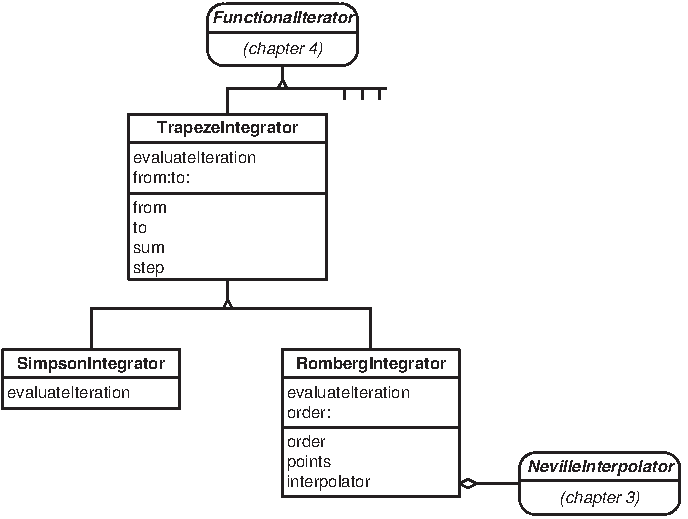
\includegraphics[width=10cm]{Figures/IntegrationClassDiagram}
\caption{Class diagram of integration classes}\label{fig:integclass}
\end{figure}
The first one, trapeze integration, is only introduced for the
sake of defining a common framework for the next two algorithms:
Simpson and Romberg integration. In general, the reader should use
Romberg's algorithm. It is fast and very precise. There are,
however, some instances where Simpson's algorithm can be faster if
high accuracy is not required.

\section{General framework --- Trapeze integration method}
\label{sec:trapeze}
Let us state it at the beginning.
One should not use the trapeze integration algorithm in practice.
The interest of this algorithm is to define a general framework for
numerical integration.
All subclasses of the class responsible for implementing the trapeze integration algorithm will reuse most the mechanisms described in this section.

The trapeze numerical integration method takes its origin in the
series expansion of an integral. This series expansion is
expressed by the Euler-Maclaurin formula shown hereafter
\cite{Bass}:
\begin{equation}
\label{eq:eulerMacLaurin}
  \int_a^b f\left(x\right)dx={b-a\over
  2}\left[f\left(a\right)+f\left(b\right)\right]-\sum_n{\left(b-a\right)^2\over
  \left(2n\right)!}B_{2n}\left[{d^{2n-1}f\left(b\right)\over dx^{2n-1}}-{d^{2n-1}f\left(a\right)\over
  dx^{2n-1}}\right],
\end{equation}
where the numbers $B_{2n}$ are the Bernouilli numbers.

The next observation is that, if the interval of integration is small enough, the series in the second term of equation \ref{eq:eulerMacLaurin} would yield a contribution negligible compared to that of the first term.
Thus, we can write:
\begin{equation}
\label{eq:approxEML}
  \int_a^b f\left(x\right)dx\approx{b-a\over
  2}\left[f\left(a\right)+f\left(b\right)\right],
\end{equation}
if $b-a$ is sufficiently small. The approximation of equation
\ref{eq:approxEML} represents the area of a trapeze whose summits
are the circled points in Figure \ref{fig:trapeze}. Finally, one
must remember the additive formula between integrals:
\begin{figure}
\centering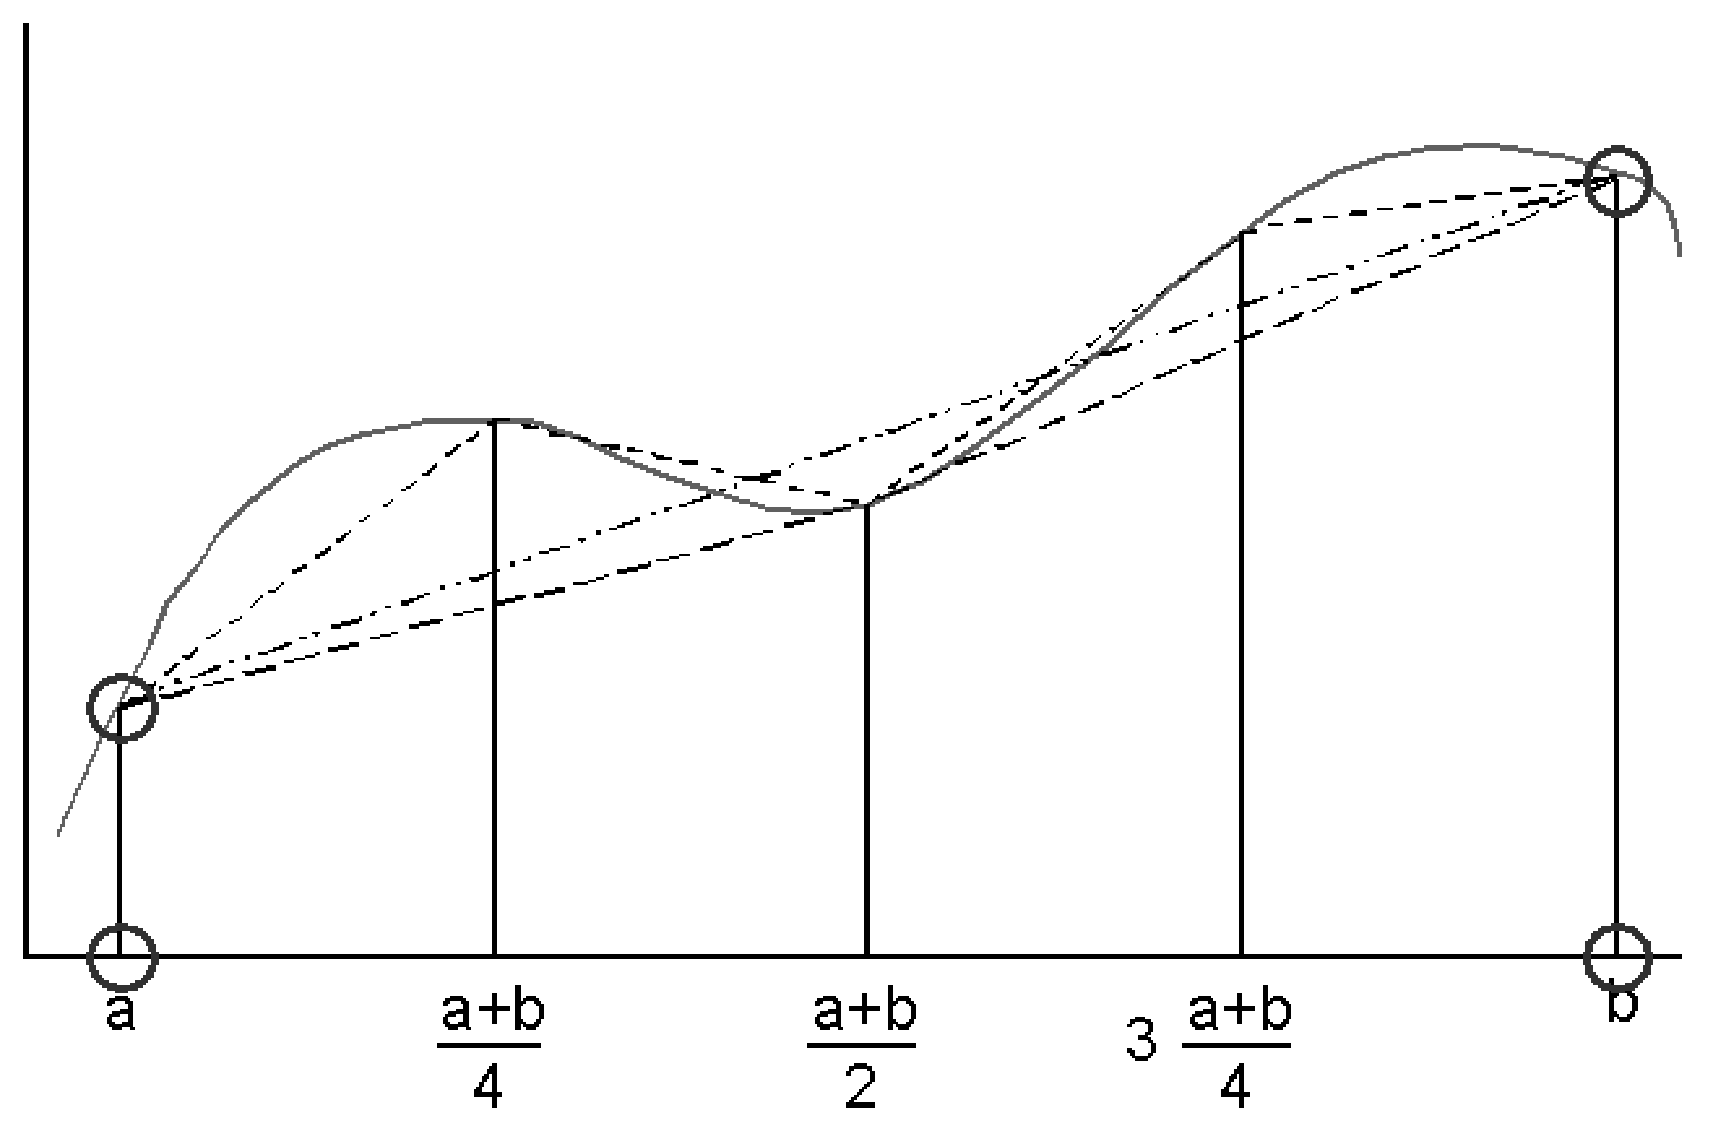
\includegraphics[width=10cm]{Figures/IntegrationGraph}
\caption{Geometrical interpretation of the trapeze integration
method}\label{fig:trapeze}
\end{figure}
\begin{equation}
\label{eq:addintegral}
  \int_a^b f\left(x\right)dx=\int_a^c f\left(x\right)dx+\int_c^b f\left(x\right)dx,
\end{equation}
for any $c$. We shall use this property by chosing a $c$ located
between $a$ and $b$.

The resulting strategy is a divide-and-conquer strategy. The
integration interval is divided until one can be sure that the
second term of equation \ref{eq:eulerMacLaurin} becomes indeed
negligible. As one would like to re-use the points at which the
function has been evaluated during the course of the algorithm,
the integration interval is halved at each iteration. The first
few steps are outlined in figure \ref{fig:trapeze}. An estimation
of the integral is obtained by summing the areas of the trapezes
corresponding to each partition.

Let $x_0^{\left(n\right)},\ldots,x_{2^n}^{\left(n\right)}$ be the
partition of the interval at iteration $n$. Let
$\epsilon^{\left(n\right)}$ be the length of each interval between
these points. We thus have:
\begin{equation}
  \left\{
  \begin{array}{lcl}
    \epsilon^{\left(n\right)} & = & {\displaystyle b-a \over\displaystyle 2^n} \\
    x_0^{\left(n\right)} & = & a \\*[0.5ex]
    x_i^{\left(n\right)} & = & a+i\epsilon^{\left(n\right)}
    \mbox{\quad for $i=1,\ldots,2^n$.}
  \end{array}
  \right.
\end{equation}
The corresponding estimation for the integral is:
\begin{equation}
\label{eq:trapezesum}I^{\left(n\right)}=\epsilon^{\left(n\right)}\left[f\left(a\right)+f\left(b\right)+2
\sum_{i=1}^{2^n-1}f\left(x_i^{\left(n\right)}\right)\right] .
\end{equation}
To compute the next estimation, it suffices to compute the value
of the function at the even values of the partition because the
odd values were already computed before. One can derive the
following recurrence relation:
\begin{equation}
\label{eq:trapeze} I^{\left(n+1\right)}={I^{\left(n\right)}\over
2}+ \epsilon^{\left(n\right)}
\sum_{i=1}^{2^n-1}f\left(x_{2i-1}^{\left(n\right)}\right),
\end{equation}
with the initial condition:
\begin{equation}
I^{\left(0\right)}={b-a \over
2}\left[f\left(a\right)+f\left(b\right)\right].
\end{equation}
Note that the sum on the right-hand side of equation
\ref{eq:trapeze} represents the sum of the function's values at
the new points of the partition.

\rubrique{End game strategy} The final question is when should the
algorithm be stopped? A real honest answer is we do not know. The
magnitude of the series in equation \ref{eq:eulerMacLaurin} is
difficult to estimate as the Bernouilli numbers become very large
with increasing $n$. An experimental way is to watch for the
change of the integral estimate In other words the absolute value
of the last variation,
$\left|I^{\left(n\right)}-I^{\left(n+1\right)}\right|$ , is
considered a good estimate of the precision. This kind of
heuristic works for most functions.

At each iteration the number of function evaluation doubles. This
means that the time spent in the algorithm grows exponentially
with the number of iterations. Thus, the default maximum number of
iteration must be kept quite low compared to that of the other
methods.

In practice, however, trapeze integration converges quite slowly
and should not be used. Why bother implementing it then? It turns
out that the more elaborate methods, Simpson and Romberg
integration, require the computation of the same sums needed by
the trapeze integration. Thus, the trapeze integration is
introduced to be the superclass of the other better integration
methods.

One must keep in mind, however, that the magnitude of the series
in equation \ref{eq:eulerMacLaurin} can become large for any
function whose derivatives of high orders have singularities over
the interval of integration. The convergence of the algorithm can
be seriously compromised for such functions. This remark is true
for the other algorithms described in this chapter. For example,
none of the algorithms is able to give a precise estimate of the
beta function using equation \ref{eq:betaint} with $x>1$ and $y<1$
(\cf section \ref{sec:betafunc}) because, for these values, the
derivatives of the function to integrate have a singularity at
$t=1$.

Another problem can come up if the function is nearly zeroes at
regular intervals. For example, evaluating the integral of the
function $f\left(x\right)={\sin\left(2^mx\right)\over x}$  from
$-\pi$ to $\pi$ for a moderate value of $m$. In this case, the
terms $I^{\left(0\right)}$ to $I^{\left(m\right)}$ will have a
null contribution. This would cause the algorithm to stop
prematurely. Such special function behavior is of course quite
rare. Nevertheless the reader must be aware of the limitations of
the algorithm. This remark is valid for all algorithms exposed in
this chapter.

\subsection{Trapeze integration --- Smalltalk implementation}
\label{sec:strapeze}
%\marginpar{Figure \ref{fig:integclass} with the box {\bf PMTrapezeIntegrator} grayed.}
The class implementing trapeze integration is a subclass of the functional iterator discussed in
section \ref{sec:iterrel}. Two instance variables are needed to
define the integration interval. Additional instance variables
must keep track of the partition of the interval and of the
successive estimations. Consequently, the class has the following
instance variables.
\begin{itemize}
\item \code{from} contains the lower limit of the integration's interval,
 \ie\ $a$,
\item \code{to} contains the lower limit of the integration's interval,
 \ie\ $b$,
\item \code{step} contains the size of the interval's partition,
 \ie\ $\epsilon^{\left(n\right)}$,
\item \code{sum} contains the intermediate sums, \ie\ $I^{\left(n\right)}$.
\end{itemize}

Although trapeze integration is not a practical algorithm, we give
an example of implementation. The reason is that the public interface used by trapeze integration is the same for all integration classes.

The example shown in the next two sections is the integration of
the inverse function. In mathematics the natural logarithm of $x$,
$\ln x$, is defined as the integral from 1 to $x$ of the inverse
function. Of course, using numerical integration is a very
inefficient way of computing a logarithm. This example, however,
allows the reader to investigate the accuracy (since the exact
solution is known) and performances of all algorithms presented in
this chapter. The interested reader should try the example for
various setting of the desired precision and look at the number of
iterations needed for a desired precision. She can also verify how
accurate is the estimated precision.

Listing \ref{lst:trapeze} shows the Smalltalk implementation of the trapeze integration method. In Smalltalk the code for the computation of the integral defining the natural logarithm is as follows:
\begin{displaycode}{Smalltalk}
| integrator ln2 ln3 |
integrator := PMTrapezeIntegrator
                 function: [ :x | 1.0 / x ] from: 1 to: 2.
ln2 := integrator evaluate.
integrator from: 1 to: 3.
ln3 := integrator evaluate.
\end{displaycode}
The line after the declaration creates a new instance of the class \code{PMTrapezeIntegrator} for the inverse function. The limits of the integration interval are set from 1 to 2 at creation time. The
third line retrieves the value of the integral. The fourth line
changes the integration interval and the last line retrieves the
value of the integral over the new integration interval.

The class \code{PMTrapezeIntegrator} is a subclass of the class
\code{PMAbstractFunctionIterator} defined in section
\ref{sec:siterrel}.

In order to create an instance you need to use class method \code{function:from:to:} to define the fucntion and the integration interval.

%The default creation class method \code{new} has been overloaded to prevent creating an object without initialized instance variables. The proper creation class method defines the function and the integration interval.

The method \code{from:to:} allows changing the integration interval
for a new computation with the same function.

Note that the initialization of the iterations (method \code{computeInitialValues}, \cf section \ref{sec:siteration}) also corresponds to the first iteration of the algorithm.
The method \code{highOrderSum} computes the sum of the right-hand side of equation \ref{eq:trapeze}.

\begin{listing}[label=lst:trapeze]{Smalltalk}
{Smalltalk implementation of trapeze integration}
PMFunctionalIterator subclass: #PMTrapezeIntegrator
   instanceVariableNames: 'from to sum step'
   classVariableNames: ''
   package: 'Math-DHB-Numerical'
\end{listing}

\begin{displaycode}{Smalltalk}
PMTrapezeIntegrator class >> defaultMaximumIterations
    ^13
\end{displaycode}

\begin{displaycode}{Smalltalk}
PMTrapezeIntegrator class >> function: aBlock from: aNumber1 to: aNumber2
    ^super new initialize: aBlock from: aNumber1 to: aNumber2
\end{displaycode}

\begin{displaycode}{Smalltalk}
PMTrapezeIntegrator >> computeInitialValues
    step := to - from.
    sum := ((functionBlock value: from) + (functionBlock value: to)) * step /2.
    result := sum.
\end{displaycode}

\begin{displaycode}{Smalltalk}
PMTrapezeIntegrator >> evaluateIteration
    | oldResult |
    oldResult := result.
    result := self higherOrderSum.
    ^ self relativePrecision: ( result - oldResult) abs
\end{displaycode}

\begin{displaycode}{Smalltalk}
PMTrapezeIntegrator >> from: aNumber1 to: aNumber2
    from := aNumber1.
    to := aNumber2
\end{displaycode}

\begin{displaycode}{Smalltalk}
PMTrapezeIntegrator >> higherOrderSum
    | x newSum |
    x := step / 2 + from.
    newSum := 0.
    [ x < to ]
        whileTrue: [ newSum := ( functionBlock value: x) + newSum.
                     x := x + step.
                   ].
    sum := ( step * newSum + sum) / 2.
    step := step / 2.
    ^ sum
\end{displaycode}

\begin{displaycode}{Smalltalk}
PMTrapezeIntegrator >> initialize: aBlock from: aNumber1 to: aNumber2
    functionBlock := aBlock.
    self from: aNumber1 to: aNumber2.
    ^ self
\end{displaycode}

\section{Simpson integration algorithm}
%\marginpar{Figure \ref{fig:integclass} with the box {\textbf SimpsonIntegrator} grayed.}

Simpson integration algorithm consists in replacing the function to integrate by a second order Lagrange interpolation polynomial\cite{Bass} (\cf section
\ref{sec:lagrange}). One can then carry the integral analytically.
Let $f\left(x\right)$ be the function to integrate. For a given
interval of integration, $\left[a,b\right]$, the function is
evaluated at the extremities of the interval and at its middle
point $c={a+b \over 2}$. As defined in equation \ref{eq:lagrange}
the second order Lagrange interpolation polynomial is then given
by:
\begin{equation}
  P_2\left(x\right)={2\over \left(b-a\right)^2}\left[\left(x-b\right)\left(x-c\right)f\left(a\right) +\left(x-c\right)\left(x-a\right)f\left(b\right) +
  \left(x-a\right)\left(x-b\right)f\left(c\right)\right].
\end{equation}
The integral of the polynomial over the interpolation interval is
given by:
\begin{equation}
\label{eq:simpson} \int_a^b P_2\left(x\right)dx={b-a \over
6}\left[f\left(a\right) + f\left(b\right) + 4 f\left(c\right)
\right].
\end{equation}
As for trapeze integration, the interval is partitioned into small
intervals. Let us assume that the interval has been divided into
subintervals. By repeating equation \ref{eq:simpson} over each
subinterval, we obtain:
\begin{equation}
\label{eq:simpsum} \int_a^b
P_2\left(x\right)dx={\epsilon^{\left(n\right)} \over
3}\left[f\left(a\right) + f\left(b\right) + 2 \sum_{i=1}^{2^{n-1}}
f\left(x_{2i-1}^{\left(n\right)}\right) + 4 \sum_{i=0}^{2^{n-1}}
f\left(x_{2i}^{\left(n\right)}\right) \right].
\end{equation}
Equation \ref{eq:simpsum} uses the notations introduced in section
\ref{sec:trapeze}. Except for the first iteration, the right-hand
side of equation \ref{eq:simpsum} can be computed from the
quantities $I^{\left(n\right)}$ defined in equation
\ref{eq:trapezesum}. Thus, we have:
\begin{equation}
  \int_a^b
P_2\left(x\right)dx={1 \over
3}\left[4I^{\left(n\right)}-I^{\left(n-1\right)}\right]
\mbox{\quad for $n>1$}
\end{equation}
This can be checked by verifying that $I^{\left(n-1\right)}$ is
equal to the first sum of equation \ref{eq:simpsum} times  and
that $I^{\left(n\right)}$  is equal to the addition of the two
sums of equation \ref{eq:simpsum} times
$\epsilon^{\left(n\right)}$. As advertised in section
\ref{sec:trapeze} we can re-use the major parts of the trapeze
algorithm: computation of the sums and partition of the
integration interval.

Like in the case of the trapeze algorithm, the precision of the
algorithm is estimated by looking at the differences between the
estimation obtained previously and the current estimation. At the
first iteration only one function point is computed. This can
cause the process to stop prematurely if the function is nearly
zero at the middle of the integration interval. Thus, a protection
must be built in to prevent the algorithm from stopping at the
first iteration.

\subsection{Simpson integration --- Smalltalk implementation}
\label{sec:sSimpson}
The class implementing Simpson algorithm is a subclass of the
class implementing trapeze integration.
The method \code{evaluateIteration} is the only method needing change.
The number of iterations is checked to prevent returning after the first
iteration.

The public interface is the same as that of the superclass.
Thus, all the examples shown in sections \ref{sec:strapeze} can be used for Simpson
algorithm by just changing the name of the class.

Listing \ref{lst:simpson} shows the complete implementation in Smalltalk.

The class \code{PMSimpsonIntegrator} is a subclass of the class
\code{PMTrapezeIntegrator} defined in section \ref{sec:strapeze}.

\begin{listing}[label=lst:simpson]{Smalltalk}
{Smalltalk implementation of the Simpson integration algorithm}
PMTrapezeIntegrator subclass: #PMSimpsonIntegrator
   instanceVariableNames: ''
   classVariableNames: ''
   package: 'Math-DHB-Numerical'
\end{listing}

\begin{displaycode}{Smalltalk}
PMSimpsonIntegrator >> evaluateIteration
| oldResult oldSum |
    iterations < 2
        ifTrue: [ self higherOrderSum.
                  ^ 1 ].
    oldResult := result.
    oldSum := sum.
    result := (self higherOrderSum * 4 - oldSum) / 3.
    ^self relativePrecision: ( result - oldResult) abs
\end{displaycode}

\section{Romberg integration algorithm}
\label{sec:romberg}
%\marginpar{Figure \ref{fig:integclass} with the box {\textbf RombergIntegrator} grayed.}
If one goes back to equation \ref{eq:eulerMacLaurin} one notices that the second term is of the
order of the square of the integration interval. Romberg's
algorithm uses this fact to postulate that $I^{\left(n\right)}$ is
a smooth function of the square of the size of interval's
partition $\epsilon^{\left(n\right)}$. Romberg's algorithm
introduces the parameter $k$ where $k-1$ is the degree of the
interpolation's polynomial\footnote{In other words, $k$ is the
number of points over which the interpolation is performed (\cf
section \ref{sec:lagrange}).}. The result of the integral is
estimated by extrapolating the series
$I^{\left(n-k\right)},\ldots,I^{\left(n\right)}$ at the value
$\epsilon^{\left(n\right)}=0$. Since we have:
\begin{equation}
\epsilon^{\left(n\right)}={\epsilon^{\left(n-1\right)} \over 2},
\end{equation}
one only needs to interpolate over successive powers of $1/4$ ,
starting with 1: 1, $1/4$, $1/16$, $1/256$, \etc. In this case,
extrapolation is safe because the value at which extrapolation is
made is very close to the end of the interval defined by the
sample points and actually becomes closer and closer with every
iteration.

Thus, Romberg's algorithm requires at least $k$ iterations. The
good news is that this algorithm converges very quickly and, in
general, only a few iterations are needed after the five initial
ones. A polynomial of $4^{\mathop{\textrm{th}}}$ degree --- that is
$k=5$ --- is generally sufficient \cite{Press}.

Extrapolation is performed using Neville's algorithm (\cf section
\ref{sec:neville}) because it computes an estimate of the error on
the interpolated value. That error estimate can then be used as
the estimate of the error on the final result.

If $k=1$ Romberg's algorithm is equivalent to trapeze integration.
If $k=2$, the interpolation polynomial is given by:
\begin{equation}
P_1\left(x\right)=y_1+{x-x_1 \over x_2-x_1}\left(y_2-y_1\right).
\end{equation}
At the $n^{\mathop{\textrm{th}}}$ iteration we have:
$y_1=I^{\left(n-1\right)}$, $y_2=I^{\left(n\right)}$ and
$x_2=x_1/4$. Thus, the interpolated value at 0 is:
\begin{equation}
P_1\left(0\right)=I^{\left(n-1\right)}+{4 \over
3}\left[I^{\left(n\right)}-I^{\left(n-1\right)}\right] ={1\over
3}\left[4I^{\left(n\right)}-I^{\left(n-1\right)}\right]
\end{equation}
Thus, for $k=2$ Romberg's algorithm is equivalent to Simpson's
algorithm. For higher order, however, Romberg's algorithm is much
more efficient than Simpson method as soon as precision is
required (\cf a comparison of the result in section
\ref{sec:intwhich}).

Using interpolation on the successive results of an iterative
process to obtain the final result is a general procedure known as
Richardson's deferred approach to the limit \cite{Press}. This
technique can be used whenever the estimated error can be
expressed as a function of a suitable parameter depending on the
iterations. The choice of the parameter, however, is critical. For
example, if one had interpolated over the size of the interval's
partition instead of its square, the method would not converge as
well\footnote{It converges at the same speed as Simpson's
algorithm. This can be verified by running the comparison programs
after changing the factor 0.25 used to compute the abscissa of the
next point into 0.5.}.

\subsection{Romberg integration --- Smalltalk implementation}
\label{sec:sromberg}
The class implementing Romberg's algorithm needs the following
additional instance variables:
\begin{itemize}
\item \code{order} the order of the interpolation, \ie\ $k$,\\
\item \code{interpolaton} an instance of Neville's interpolation class,\\
\item \code{points} an \code{OrderedCollection} containing the most recent sum estimates,
\ie\ $I^{\left(n-k\right)},\ldots,I^{\left(n\right)}$.\\
\end{itemize}
The method \code{evaluateIteration} (\cf section \ref{sec:iteration}) contains the entire algorithm. At each iteration the collection of point receives a new point with an
abscissa equal to the quarter of that of the last point and an
ordinate equal to the next sum estimate . If not enough points are
available, the method returns a precision such that the iterative
process will continue. Otherwise, the extrapolation is performed.
After the result of the extrapolation has been obtained the oldest
point is removed. In other words, the collection of points is used
as a last-in-last-out list with a constant number of elements
equal to the order of the interpolation. Of the two values
returned by Neville's interpolation (\cf section \ref{sec:neville}), the interpolated value is stored in the result
and the error estimate is returned as the precision for the other.

Listing \ref{lst:romberg} shows the Smalltalk implementation of Romberg's algorithm. The class \code {PMRombergIntegrator} is a subclass of the class \code{PMTrapezeIntegrator} defined in section \ref{sec:strapeze}.

The class method \code{defaultOrder} defines the default order to
5. This method is used in the method initialize so that each newly
created instance is created with the default interpolation order.
The method \code{order:} allows changing the default order if
needed.

The sample points defining the interpolation are stored in an \code{OrderedCollection}. This collection is created in the method \code{computeInitialValues}.
Since the number of points will never exceed the order of the interpolation the maximum size is preset when the collection is created.
The method \code{computeInitialValues} also creates the object in charge of performing the interpolation and it stores the first point in the collection of sample points.
\begin{listing}[label=lst:romberg]{Smalltalk}
{Smalltalk implementation of Romberg integration}
PMTrapezeIntegrator subclass: #PMRombergIntegrator
   instanceVariableNames: 'order points interpolator'
   classVariableNames: ''
   package: 'Math-DHB-Numerical'
\end{listing}

\begin{displaycode}{Smalltalk}
PMRombergIntegrator class >> defaultOrder
    ^5
\end{displaycode}

\begin{displaycode}{Smalltalk}
PMRombergIntegrator >> computeInitialValues
    super computeInitialValues.
    points := OrderedCollection new: order.
    interpolator := PMNevilleInterpolator points: points.
    points add: 1 @ sum
\end{displaycode}

\begin{displaycode}{Smalltalk}
PMRombergIntegrator >> evaluateIteration
    | interpolation |
    points addLast: (points last x * 0.25) @ self higherOrderSum.
    points size < order
        ifTrue: [ ^1].
    interpolation := interpolator valueAndError: 0.
    points removeFirst.
    result := interpolation at: 1.
    ^self relativePrecision: ( interpolation at: 2) abs
\end{displaycode}

\begin{displaycode}{Smalltalk}
PMRombergIntegrator >> initialize
    order := self class defaultOrder.
    ^ super initialize
\end{displaycode}

\begin{displaycode}{Smalltalk}
PMRombergIntegrator >> order: anInteger
    anInteger < 2
        ifTrue: [
           self error: 'Order for Romberg integration must be 
                                                larger than 1'].
    order := anInteger
\end{displaycode}

\section{Evaluation of open integrals}
An open integral is an integral for which the function to
integrate cannot be evaluated at the boundaries of the integration
interval. This is the case when one of the limit is infinite or
when the function to integrate has a singularity at one of the
limits. If the function to integrate has one or more singularity
in the middle of the integration interval, the case can be reduced
to that of having a singularity at the limits using the additive
formula between integrals \ref{eq:addintegral}. Generalization of
the trapeze algorithm and the corresponding adaptation of
Romberg's algorithm can be found in \cite{Press}.

\rubrique{Bag of tricks} My experience is that using a suitable
change of variable can often remove the problem. In particular,
integrals whose integration interval extends to infinity can be
rewritten as integrals over a finite interval. We give a few
examples below.

For an integral starting from minus infinity, a change of variable
$t={1 \over x}$ can be used as follows:
\begin{equation}
\label{eq:inftyvarchg}
  \int_{-\infty}^a f\left(x\right)dx= \int_{1\over a}^0 f\left({1\over
  t}\right){dt\over t^2}\mbox{\quad for $a<0$.}
\end{equation}
For such integral to be defined, the function must vanish at minus
infinity faster than $x^2$. This means that:
\begin{equation}
  \lim_{t \to 0}{1\over t^2}f\left({1\over
  t}\right)=0.
\end{equation}
If $a>0$, the integration must be evaluated in two steps, for
example one over the interval $\left]-\infty,-1\right]$ using the
change of variable of equation \ref{eq:inftyvarchg} and one over
the interval $\left[-1,a\right]$ using the original function.

For integral ending at positive infinity the same change of
variable can also be made. However, if the interval of integration
is positive, the change of variable $t=e^{-x}$ can be more
efficient. In this case, one makes the following transformation:
\begin{equation}
\int_a^{+\infty} f\left(x\right)dx=\int_0^{e^{-a}}f\left(-\ln t
\right){dt \over t}\mbox{\quad for $a>0$}.
\end{equation}
For this integral to be defined one must have:
\begin{equation}
  \lim_{t \to 0}{1\over t}f\left(\ln
  t\right)=0.
\end{equation}
By breaking up the interval of integration is several pieces one
can chose a change of variable most appropriate for each piece.

\section{Which method to chose?}
\label{sec:intwhich} An example comparing the results of the three
algorithms is given in section \ref{sec:sintcompar} for Smalltalk.
The function to integrate is the inverse function in both cases. The integration
interval is from 1 to 2 so that the value of the result is known,
namely $\ln 2$. Integration is carried for various values of the
desired precision. The reader can then compare the attained
precision (both predicted and real) and the number of
iterations\footnote{Note that the number of iterations printed in
the examples in one less than the real number of iterations
because the first iteration is performed in the set-up phase of
the iterative process.} required for each algorithm. Let us recall
that the number of required function evaluations grows
exponentially with the number of iterations.

The results clearly show that the trapeze algorithm is ruled out
as a practical method. As advertised in section \ref{sec:trapeze}
it is not converging quickly toward a solution.

Romberg's algorithm is the clear winner. At given precision, it
requires the least number of iterations. This is the algorithm of
choice in most cases.

Simspon's algorithm may be useful if the required precision is not
too high and if the time to evaluate the function is small
compared to the interpolation. In such cases Simspon's algorithm
can be faster than Romberg's algorithm.

Section \ref{sec:sintcompar} give some sample code the reader can use to
investigate the various integration algorithms.
The results of the code execution are shown in table \ref{tb:intcompar}.
The columns of this table are:
\begin{itemize}
\item $\epsilon_{\mathop{\textrm{max}}}$ the desired precision,\\
\item $n$ the number of required iterations; let us recall that the
corresponding number of function's evaluations is $2^{n+1}$,\\
\item $\tilde{\epsilon}$ the estimated precision of the result,\\
\item $\epsilon$ the effective precision of the result, that is the absolute value
of the difference between the result of the integration algorithm and the true result.\\
\end{itemize}

\begin{table}[h]
  \centering
  \caption{Comparison between integration algorithms}\label{tb:intcompar}
\vspace{1 ex}
\begin{tabular}{|l|l|l|l|l|l|l|l|l|l|} \hline
  &\multicolumn{3}{c|}{\textbf{Trapeze algorithm}} &\multicolumn{3}{c|}{\textbf{Simpson algorithm}}&\multicolumn{3}{c|}{\textbf{Romberg algorithm}}  \\ \hline
  $\epsilon_{\mathop{\textrm{max}}}$ & $n$ & $\tilde{\epsilon}$ & $\epsilon$ & $n$ & $\tilde{\epsilon}$ & $\epsilon$ & $n$ & $\tilde{\epsilon}$ & $\epsilon$
  \\ \hline
$10^{-5}$&8&$4.1\cdot 10^{-6}$&$9.5\cdot 10^{-7}$&4&$9.9\cdot
10^{-6}$&$4.7\cdot 10^{-7}$&4&$1.7\cdot 10^{-9}$&$1.4\cdot
10^{-9}$\\ \hline $10^{-7}$&11&$6.4\cdot 10^{-8}$&$1.5\cdot
10^{-8}$&6&$4.0\cdot 10^{-8}$&$1.9\cdot 10^{-9}$&4&$1.7\cdot
10^{-9}$&$1.4\cdot 10^{-9}$\\ \hline $10^{-9}$ &15&$2.5\cdot
10^{-10}$&$5.8\cdot 10^{-11}$&8&$1.5\cdot 10^{-10}$&$7.3\cdot
10^{-12}$&5&$1.4\cdot 10^{-11}$&$3.7\cdot 10^{-12}$\\ \hline
$10^{-11}$ &18&$3.9\cdot 10^{-12}$&$9.0\cdot 10^{-13}$&9&$9.8\cdot
10^{-12}$&$5.7\cdot 10^{-13}$&6&$7.6\cdot 10^{-14}$&$5.7\cdot
10^{-15}$\\ \hline $10^{-13}$&21&$4.8\cdot 10^{-14}$&$2.8\cdot
10^{-14}$&11&$3.8\cdot 10^{-14}$&$1.9\cdot 10^{-15}$&6&$7.6\cdot
10^{-14}$&$5.7\cdot 10^{-15}$\\ \hline
\end{tabular}
\end{table}

\subsection{Smalltalk comparison}
\label{sec:sintcompar} The script of Listing \ref{lst:intcompare}
can be executed as such in a playground window.

The function to integrate is specified as a block closure as
discussed in section \ref{sec:stFunction}.
\begin{listing}[label=lst:intcompare]{Smalltalk}
{Smalltalk comparison script for integration algorithms}
| a b  integrators |
a := 1.0.
b := 2.0.
integrators := Array with: (
            (PMTrapezeIntegrator function: [ :x | 1.0 / x]) from: a to: b)
            with: (
            (PMSimpsonIntegrator function: [ :x | 1.0 / x]) from: a to: b)
            with: (
            (PMRombergIntegrator function: [ :x | 1.0 / x]) from: a to: b).
#(1.0e-5 1.0e-7 1.0e-9 1.0e-11 1.0e-13) do: 
[ :precision |
   Transcript cr; cr; nextPutAll: '===> Precision: '.
   precision printOn: Transcript.
   integrators do:
      [ :integrator |
      Transcript cr; nextPutAll: '*****   ', integrator class name,':'; cr.
      integrator desiredPrecision: precision.
      Transcript nextPutAll: 'Integral of 1/x from '.
      a printOn: Transcript.
      Transcript nextPutAll: ' to '.
      b printOn: Transcript.
      Transcript nextPutAll: ' = '.
      integrator evaluate printOn: Transcript.
      Transcript nextPutAll: ' +- '.
      integrator precision printOn: Transcript.
      Transcript cr; nextPutAll: ' ( '.
      integrator iterations printOn: Transcript.
      Transcript nextPutAll: ' iterations, true error = '.
      ( integrator result - 2 ln) printOn: Transcript.
      Transcript nextPutAll: ')'; cr].
   Transcript flush.
]
\end{listing}


%\ifx\wholebook\relax\else\end{document}\fi

%\ifx\wholebook\relax\else
%\documentclass[twoside]{book}

%\usepackage[active]{srcltx}
%\usepackage[LY1]{fontenc}
%\usepackage{url}
\makeatletter
\def\url@leostyle{%
  \@ifundefined{selectfont}{\def\UrlFont{\sf}}{\def\UrlFont{\sffamily}}}
\makeatother
% Now actually use the newly defined style.
\urlstyle{leo}

\usepackage{graphicx}
\def\etc{{\textit{etc}}}
\def\eg{{\textit{e.g.}}}
\def\ie{{\textit{i.e.}}}
\def\cf{{\textit{c.f.}}\ }
\def\erf{\mathop{\textrm{erf}}}
\def\sign{\mathop{\textrm{sign}}}
\def\prob{\mathop{\textrm{Prob}}}
\def\var{\mathop{\textrm{var}}}
\def\mod{\mathop{\textrm{mod}}}
\def\cor{\mathop{\textrm{cor}}}
\def\cov{\mathop{\textrm{cov}}}
\def\cl{\mathop{\textrm{CL}}}
\def\kg{\mathop{\textrm{Kg}}}
\def\patstyle#1{{\textsc #1}}
\def\th{^{\mathop{\textrm{th}}}}
%\def\st#1{^{\mathop{\rm #1}}}
\def\note#1{\begin{quote}{\textbf{Note:}} #1\end{quote}}
\def\braket#1{\left\langle #1\right\rangle}
\def\order#1{\let\o=#1$\mathcal{O}$\ifx\o 1$\left(n\right)$\else$\left(n^{#1}\right)$\fi}
%\newtheorem{privListing}{Listing}[chapter]
%\newenvironment{listing}{\vskip 3ex\hrule\vskip 1ex\begin{privListing}}{\end{privListing}\hrule\vskip 1ex}
\newtheorem{privExample}{Code example}[chapter]
\newenvironment{codeExample}{\begin{privExample}\begin{quote}\tt}{\end{quote}\end{privExample}}
\def\relboxl#1#2{\hbox to #1\hsize{#2\hfil}}
\def\relboxc#1#2{\hbox to #1\hsize{\hfil #2\hfil}}
\def\relboxr#1#2{\hbox to #1\hsize{\hfil #2}}
\def\transpose#1{\textbf{#1}^{\mathop\textrm{T}}}
\def\inverse#1{\textbf{#1}^{-1}}
%\def\tm{$^{\mathop{\rm TM}}$}
\def\tm{ }
\newenvironment{mainEquation}{\marginpar[\vspace{3 ex} Main
equation$\Rightarrow$]{\vspace{3 ex}$\Leftarrow$Main
equation}\begin{equation}}{\end{equation}}
\def\rubrique#1{\paragraph{#1}\hfil\par\noindent}

%\begin{document}
%\fi

\chapter{Series}
\label{ch:series}
\begin{flushright}
{\textsl On ne peut pas partir de l'infini, on peut y
aller.}\footnote{One cannot start at infinity; one can reach it,
however.}\\ Jules Lachelier
\end{flushright}
\vspace{1 ex} Whole families of functions are defined with
infinite series expansion or a continued fraction. Before the
advent of mechanical calculators, a person could earn a Ph.D. in
mathematics by publishing tabulated values of a function evaluated
by its series expansion or continued fraction. Some people
developed a talent to perform such tasks.

Some reported stories make the task of evaluating series sound
like a real business. A German nobleman discovered that one of its
peasants had a talent for numbers. He then housed him in his
mansion and put him to work on the calculation of a table of
logarithms. The table was published under the nobleman's
name\cite{Ifrah}.

Nowadays we do not need to look for some talented peasant, but we
still publish the result of computations made by other than
ourselves. Overall computers are better treated than peasants
were, though$\ldots$

\section{Introduction}
It will not come as a surprise to the reader that the computation
of infinite series is made on a computer by computing a sufficient
but finite number of terms. The same is true for continued
fractions. Thus, the computation of infinite series and continued
fractions uses the iterative process framework described in
chapter \ref{ch:iteration}. In this case the iteration consists of
computing successive terms.

The present chapter begins by exposing a general framework on how
to compute infinite series and continued fractions. Then, we show
two examples of application of this framework by implementing two
functions, which are very important to compute probabilities: the
incomplete gamma function and the incomplete beta function.

Figure \ref{fig:StSeriesClass} shows the class diagram of the Smalltalk
implementation.

\begin{figure}
\centering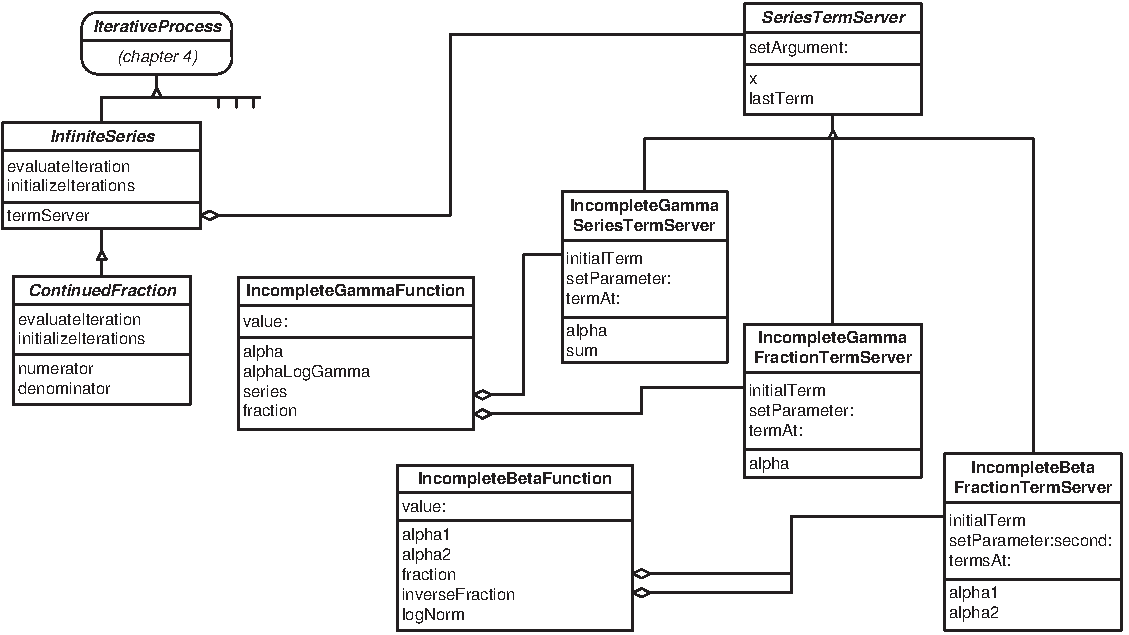
\includegraphics[width=11cm]{Figures/SeriesClassDiagram}
\caption{Smalltalk class diagram for infinite series and continued
fractions}\label{fig:StSeriesClass}
\end{figure}

The Smalltalk implementation uses two general-purpose classes to
implement an infinite series and a continued fraction
respectively. Each class then use a \patstyle{Strategy} pattern
class \cite{GoF} to compute each term of the expansion.

\section{Infinite series}
Many functions are defined with an infinite series, that is a sum
of an infinite number of terms. The most well known example is the
series for the exponential function:
\begin{equation}
  e^x=\sum_{n=0}^{\infty}{x^n \over n!}.
\end{equation}
For such a series to be defined, the terms of the series must
become very small as the index increases. If that is the case an
infinite series may be used to evaluate a function, for which no
closed expression exists. For this to be practical, however, the
series should converge quickly so that only a few terms are
needed. For example, computing the exponential of 6 to the
precision of an IEEE 32 bit floating number requires nearly 40
terms. This is clearly not an efficient way to compute the
exponential.

Discussing the convergence of a series is outside of the scope of
this book. Let us just state that in general numerical convergence
of a series is much harder to achieve than mathematical
convergence. In other words the fact that a series is defined
mathematically does not ensure that it can be evaluated
numerically.

A special remark pertains to alternating series. In an alternating
series the signs of consecutive terms are opposite. Trigonometric
functions have such a series expansion. Alternating series have
very bad numerical convergence properties: if the terms are large
rounding errors might suppress the convergence altogether. If one
cannot compute the function in another way it is best to compute
the terms of an alternating series in pairs to avoid rounding
errors.

In practice, a series must be tested for quick numerical
convergence prior to its implementation. As for rounding errors
the safest way is to do this experimentally, that is, print out
the terms of the series for a few representative\footnote{By {\textsl
representative}, I mean either values, which are covering the
domain over which the function will be evaluated, or values, which
are suspected to give convergence problems.} values of the
variable. In the rest of this chapter we shall assume that this
essential step has been made.

To evaluate an infinite series, one carries the summation until
the last added term becomes smaller than the desired precision.
This kind of logic is quite similar to that of an iterative
process. Thus, the object used to compute an infinite series
belongs to a subclass of the iterative process classe discussed in
chapter \ref{ch:iteration}.

\subsection{Infinite series --- Smalltalk  implementation}
\label{sec:sseries}
%\marginpar{Figure \ref{fig:StSeriesClass} with the boxes {\bf InfiniteSeries} and {\bf SeriesTermServer} grayed.}
Listing \ref{lst:infseries} shows a general Smalltalk
implementation of a class evaluating an infinite series. The class
being abstract, we do not give examples here. Concrete examples
are given in section \ref{sec:sincgamma}.

The Smalltalk implementation uses a \patstyle{Strategy} pattern.
The class \code{PMInfiniteSeries} is a subclass of the class \code{IterativeProcess}, discussed in section \ref{sec:siteration}.
This class does not implement the algorithm needed to compute the
terms of the series directly. It delegates this responsibility to
an object stored in the instance variable \code{termServer}. Two
hook methods, \code{initialTerm} and \code{termAt:} are used to
obtain the terms of the series from the term server object.

The method \code{evaluateIteration} uses the method \code{precisionOf:relativeTo:} to return a relative precision as discussed in section \ref{sec:siterrel}.

To implement a specific series, an object of the class \code{PMInfiniteSeries} is instantiated with a specific term server. A concrete example will be shown in section \ref{sec:sincgamma}.

Because of its generic nature, the class \code{PMInfiniteSeries}
does not implement the function behavior described in section
\ref{sec:stFunction} (method \code{value:}).
It is the responsibility of each object combining an infinite series with a
specific term server to implement the function behavior.
An example is given in section \ref{sec:sincgamma}.

\begin{listing}[label=lst:infseries]{Smalltalk}
{Smalltalk implementation of an infinite series}
PMIterativeProcess subclass: #PMInfiniteSeries
   instanceVariableNames: 'termServer'
   classVariableNames: ''
   package: 'Math-Series'
\end{listing}

\begin{displaycode}{Smalltalk}
PMInfiniteSeries class >> server: aTermServer
    ^self new initialize: aTermServer
\end{displaycode}

\begin{displaycode}{Smalltalk}
PMInfiniteSeries >> evaluateIteration
    | delta |
    delta := termServer termAt: iterations.
    result := result + delta.
    ^ self precisionOf: delta abs relativeTo: result abs
\end{displaycode}

\begin{displaycode}{Smalltalk}
PMInfiniteSeries >> initialize: aTermServer
    termServer := aTermServer.
    ^ self
\end{displaycode}

\begin{displaycode}{Smalltalk}
PMInfiniteSeries >> initializeIterations
    result := termServer initialTerm
\end{displaycode}

The computation of the terms of the series is delegated to an
object instantiated from a server class. The abstract server class
is called \code{PMInfiniteSeriesTermServer}. It is responsible to
compute the terms at each iteration. This class receives the
argument of the function defined by the series, which is kept in
the instance variable \code{x}.
The instance variable \code{lastTerm} is provided to keep the last computed term since the next term can often be computed from the previous one.
The code of this abstract class is shown in Listing 44.
\begin{listing}[label=lst:termserver]{Smalltalk}
{Smalltalk implementation of a term server}
Object subclass: #PMSeriesTermServer
   instanceVariableNames: 'x lastTerm'
   classVariableNames: ''
   package: 'Math-DHB-Numerical'
\end{listing}

\begin{displaycode}{Smalltalk}
PMSeriesTermServer >> setArgument: aNumber
    x := aNumber asFloat
\end{displaycode}

\section{Continued fractions}
\label{sec:contfractions}
A continued fraction is an infinite series of cascading fractions of the following form:
\begin{equation}
\label{eq:contfractions}
  f\left( x\right)=b_0+{a_1 \over\displaystyle b_1+
  {\strut a_2 \over\displaystyle b_2+{\strut a_3 \over\displaystyle b_3+
  {\strut a_4 \over\displaystyle b_4+\cdots}}}}
\end{equation}
In general, both sets of coefficients $a_0,\ldots$ and
$b_0,\ldots$ depend on the function's argument $x$. This
dependence in implicit in equation \ref{eq:contfractions} to keep
the notation simple. Since the above expression is quite awkward
to read - besides being a printer's nightmare - one usually uses a
linear notation as follows \cite{AbrSteg}, \cite{Press}:
\begin{equation}
\label{eq:contfractionsline}
  f\left( x\right)=b_0+{a_1 \over b_1+}{a_2 \over b_2+}{a_3 \over b_3+}{a_4 \over
  b_4+}\cdots
\end{equation}
The problem in evaluating such a fraction is that, {\textit a priori},
one must begin the evaluation from the last term. Fortunately,
methods allowing the evaluation from the beginning of the
fractions have been around since the seventeen's century. A
detailed discussion of several methods is given in \cite{Press}.
In this book, we shall only discuss the modified Lentz' method
which has the advantage to work for a large class of fractions.

Implementing the other methods discussed in \cite{Press} is left
as an exercise to the reader. The corresponding classes can be
subclassed from the classes found in this chapter.

In 1976, Lentz proposed the following two auxiliary series:
\begin{equation}
  \left\{{
  \begin{array}{lcl}
    C_0 & = & b_0,\\
    D_0 & = & 0, \\
    C_n & = & {a_n \over C_{n-1}}+b_n\mbox{\quad for $n>0$}, \\
    D_n & = & {1 \over a_n D_{n-1}+b_n}\mbox{\quad for $n>0$}.
  \end{array}
  }\right.
\end{equation}
These two series are used to construct the series:
\begin{equation}
  \left\{{
  \begin{array}{lcl}
    f_0 & = & C_0,\\
    f_n & = & f_{n-1}C_n D_n. \\
  \end{array}
  }\right.
\end{equation}
One can prove by induction that this series converges toward the
continued fraction as $n$ gets large.

In general continued fractions have excellent convergence
properties. Some care, however, must be given when one of the
auxiliary terms $C_n$ or $1/D_n$ become nearly zero\footnote{That
is, a value which is zero within the precision of the numerical
representation.}. To avoid rounding errors, Thompson and Barnett,
in 1986, proposed a modification of the Lentz method in which any
value of the coefficients smaller than a small floor value is
adjusted to the floor value \cite{Press}. The floor value is
chosen to be the machine precision of the floating-point
representation (instance variable \code{smallNumber} described in
section \ref{sec:findprecision}).

In terms of architecture, the implementation of a continued
fraction is similar to that of the infinite series.

\subsection{Continued fractions --- Smalltalk  implementation}
%\marginpar{Figure \ref{fig:StSeriesClass} with the box {\textbf ContinuedFraction} grayed.}
Listing \ref{lst:contfractions} shows the implementation of a continued fraction in Smalltalk.

The class \code{PMContinuedFraction} is built as a subclass of the class \code{PMInfiniteSeries}.
Thus, it uses also the \patstyle{Strategy} pattern.

The method \code{limitedSmallValue:} implements the prescription of Thompson and Barnett.
\begin{listing}[label=lst:contfractions]{Smalltalk}
{Smalltalk implementation of a continued fraction}
PMInfiniteSeries subclass: #PMContinuedFraction
   instanceVariableNames: 'numerator denominator'
   classVariableNames: ''
   package: 'Math-Series'
\end{listing}

\begin{displaycode}{Smalltalk}
PMContinuedFraction >> evaluateIteration
    | terms delta |
    terms := termServer termsAt: iterations.
    denominator := 1 / (self limitedSmallValue: ((terms at: 1) * denominator + (terms at: 2))).
    numerator := self limitedSmallValue: ((terms at: 1) / numerator + (terms at: 2)).
    delta := numerator * denominator.
    result := result * delta.
    ^ (delta - 1) abs
\end{displaycode}

\begin{displaycode}{Smalltalk}
PMContinuedFraction >> initializeIterations
    numerator := self limitedSmallValue: termServer initialTerm.
    denominator := 0.
    result := numerator
\end{displaycode}

\begin{displaycode}{Smalltalk}
limitedSmallValue: aNumber
    ^aNumber abs < PMFloatingPointMachine new smallNumber
            ifTrue: [ PMFloatingPointMachine new smallNumber ]
            ifFalse: [ aNumber ]
\end{displaycode}

\section{Incomplete Gamma function}
\label{sec:incGamma} The incomplete gamma function is the integral
of a gamma distribution. It is used in statistics to evaluate the
probability of finding a measurement larger than a given value
when the measurements are distributed according to a gamma
distribution. In particular, the incomplete gamma function is used
to compute the confidence level of $\chi^2$ values when assessing
the validity of a parametric fit. Several examples of use of this
function will be introduced in chapters \ref{ch:statistics} and
\ref{ch:estimation}.

Figure \ref{fig:incGamma} shows the incomplete gamma function
(solid line) and its corresponding probability density function
(dotted line) for $\alpha=2.5$.
\begin{figure}
\centering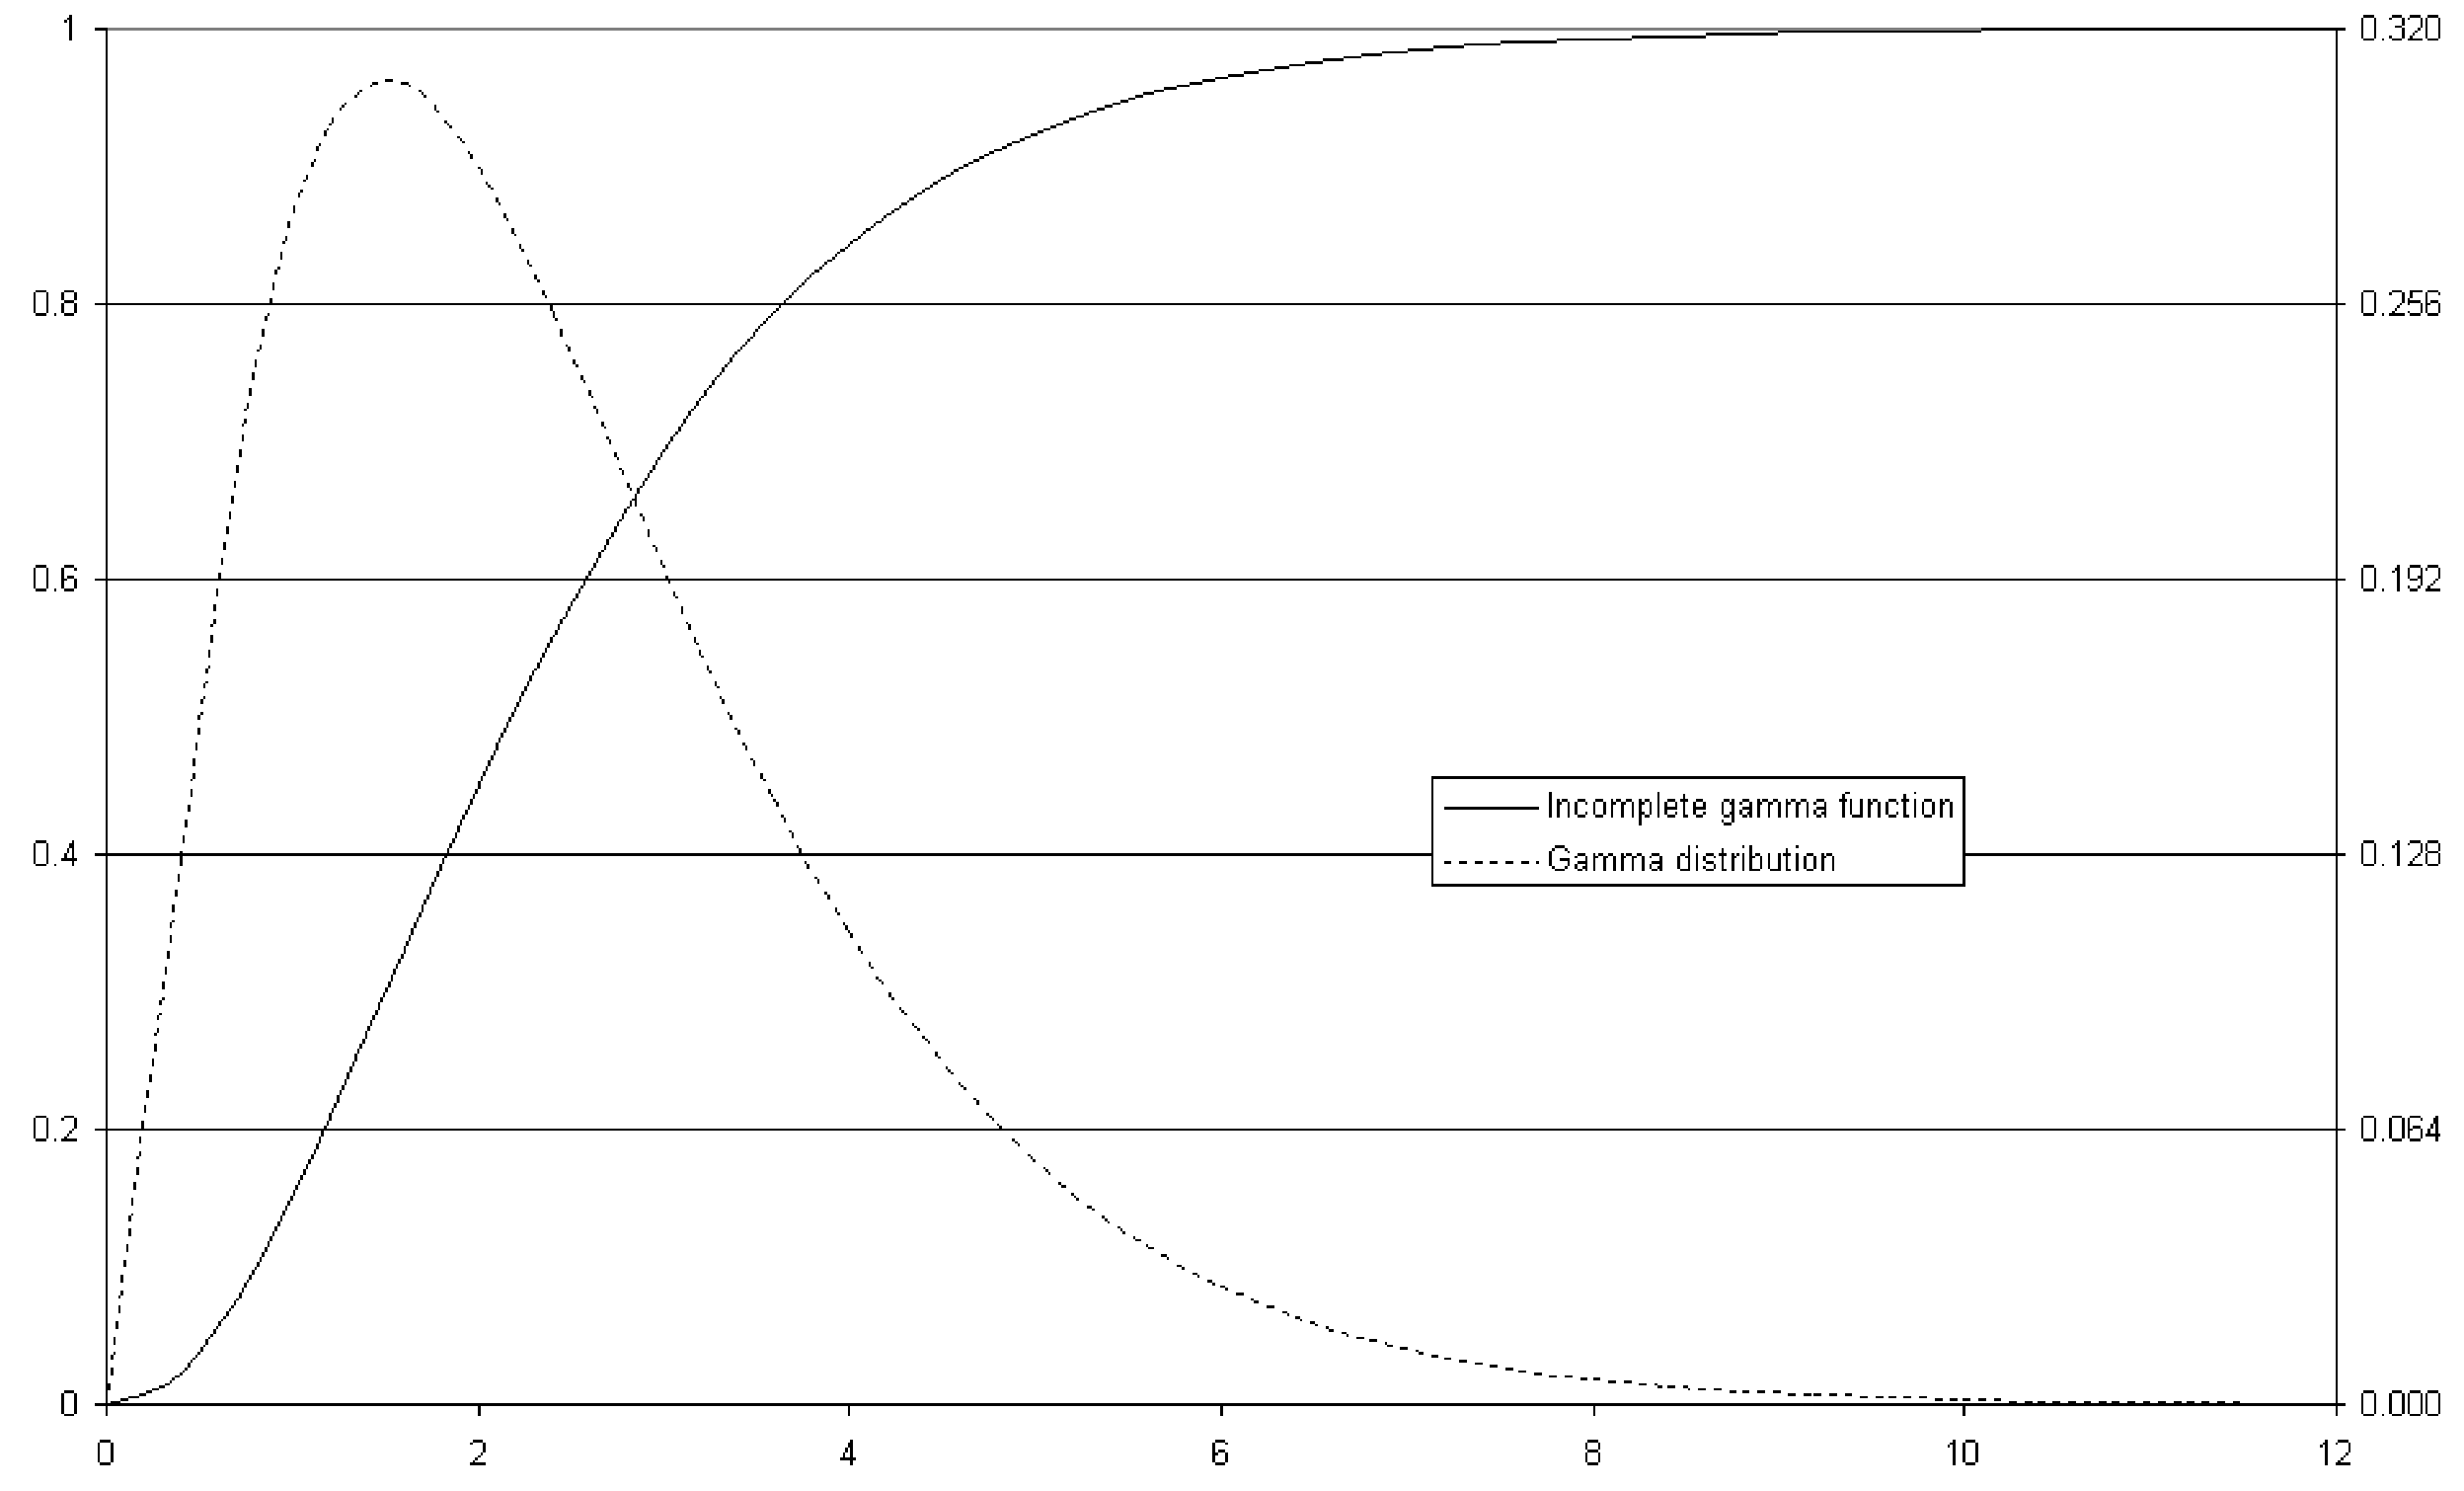
\includegraphics[width=10cm]{Figures/IncompleteGammaFunction}
\caption{The incomplete gamma function and the gamma distribution}\label{fig:incGamma}
\end{figure}

The gamma distribution is discussed in section \ref{sec:gammadist}. The $\chi^2$ confidence level is discussed in section \ref{sec:chitest}. General $\chi^2$ fits are discussed in
section \ref{sec:lsfnonlin}.

\subsection{Mathematical definitions}
\label{sec:incgamma} The incomplete gamma function is defined by
the following integral:
\begin{equation}
  \Gamma\left(x,\alpha\right)={1\over\Gamma\left(\alpha\right)}
  \int_0^x t^{\alpha -1} e^{-t} dt.
\end{equation}
Thus, the value of the incomplete gamma function lies between 0
and 1. The function has one parameter $\alpha$. The incomplete
gamma function is the distribution function of a gamma probability
density function with parameters $\alpha$ and 1 (\cf section
\ref{sec:gammadist} for a description of the gamma distribution
and its parameters). This integral can be expressed as the
following infinite series \cite{AbrSteg}:
\begin{equation}
\label{eq:incgammaser}
  \Gamma\left(x,\alpha\right)={e^{-x}x^\alpha\over\Gamma\left(\alpha\right)}
  \sum_{n=0}^{\infty}{\Gamma\left(\alpha\right) \over
  \Gamma\left(\alpha+1+n\right)}x^n.
\end{equation}
Written in this form we can see that each term of the series can
be computed from the previous one. Using the recurrence formula
for the gamma function --- equation \ref{eq:gammarec} in section
\ref{sec:gammafunc} --- we have:
\begin{equation}
\label{eq:incgammaserterm}
  \left\{{
  \begin{array}{lcl}
    a_0 & = & {1\over\alpha},\\
    a_n & = & {x\over\alpha+1+n}a_{n-1}.
  \end{array}
  }\right.
\end{equation}
The series in equation \ref{eq:incgammaser} converges well for
$x<\alpha+1$.

The incomplete gamma function can also be written as
\cite{AbrSteg}:
\begin{equation}
\label{eq:incgammafract}
  \Gamma\left(x,\alpha\right)={e^{-x}x^\alpha\over\Gamma\left(\alpha\right)}
  {1 \over F\left(x-\alpha+1,\alpha\right)},
\end{equation}
where $F\left(x,\alpha\right)$ is the continued fraction:
\begin{equation}
  F\left(x,\alpha\right)=x+{1\left(\alpha -1\right)\over x+2+}
  {2\left(\alpha -2\right)\over x+4+}
  {3\left(\alpha -3\right)\over x+6+}\ldots
\end{equation}
Using the notation introduced in equation
\ref{eq:contfractionsline} in section \ref{sec:contfractions} the
terms of the continued fraction are given by the following
expressions:
\begin{equation}
\label{eq:incgammafractterm}
  \left\{{
  \begin{array}{lcl}
    b_n & = & x-\alpha+2n\mbox{\quad for $n=0,1,2,\ldots$}\\
    a_n & = &n\left(\alpha-n\right)\mbox{\quad for $n=1,2,\ldots$}
  \end{array}
  }\right.
\end{equation}
It turns out that the continued fraction in equation
\ref{eq:incgammafract} converges for $x>\alpha+1$ \cite{Press},
that is, exactly where the series expansion of equation
\ref{eq:incgammaser} did not converge very well. Thus, the
incomplete gamma function can be computed using one of the two
methods depending on the range of the argument.

The reader will notice that equations \ref{eq:incgammaser} and
\ref{eq:incgammafract} have a common factor. The denominator of
that factor can be evaluated in advance in logarithmic form to
avoid floating-point overflow (\cf discussion in section
\ref{sec:gammafunc}). For each function evaluation the entire
factor is computed in logarithmic form to reduce rounding errors.
Then it is combined with the value of the series or the continued
fraction to compute the final result.

To avoid a floating-point error when evaluating the common factor,
the value of the incomplete gamma function at $x=0$ --- which is
of course 0 --- must be returned separately.

\subsection{Incomplete Gamma function --- Smalltalk  implementation}
\label{sec:sincgamma}
%\marginpar{Figure \ref{fig:StSeriesClass} with the boxes {\bf IncompleteGammaFunction}, {\ttextt IncompleteGammaSeriesTermServer} and {\tt IncompleteGammaFractionTermServer} grayed.}
Three classes are needed to implement the incomplete gamma function in Smalltalk.
The class \code{PMIncompleteGamaFunction} is in charge of
computing the function itself. This is the object, which responds
to the method \code{value:} to provide a function-like behavior to
the object. It is shown in Listing \ref{lst:incgamma} and has the
following instance variables.
\begin{itemize}
\item \code{alpha} contains the function's parameter, \ie\ $\alpha$,
\item \code{alphaLogGamma} used to cache the value of $\Gamma\left(\alpha\right)$ for efficiency
purposes,
\item \code{series} contains the infinite series associated to the function,
\item \code{fraction} contains the continued fraction  associated to the
function.
\end{itemize}
The instance variables \code{series} and \code{fraction} are
assigned using lazy initialization.

Depending on the range of the argument, the class delegates the
rest of the computing to either a series or a continued fraction.
In each case, a term server class provides the computation of the
terms.
They are shown in listings \ref{lst:incgammasterm} and \ref{lst:incgammafterm}.

\begin{listing}[label=lst:incgamma]{Smalltalk}
{Smalltalk implementation of the incomplete gamma function}
Object subclass: #PMIncompleteGammaFunction
   instanceVariableNames: 'alpha alphaLogGamma series fraction'
   classVariableNames: ''
   package: 'Math-DistributionGamma'
\end{listing}

\begin{displaycode}{Smalltalk}
PMIncompleteGammaFunction class >> shape: aNumber
   ^self new initialize: aNumber
\end{displaycode}

\begin{displaycode}{Smalltalk}
PMIncompleteGammaFunction >> evaluateFraction: aNumber
    fraction isNil 
        ifTrue: 
            [fraction := PMIncompleteGammaFractionTermServer new.
            fraction setParameter: alpha].
    fraction setArgument: aNumber.
    ^(PMContinuedFraction server: fraction)
        desiredPrecision: PMFloatingPointMachine new defaultNumericalPrecision;
        evaluate
\end{displaycode}

\begin{displaycode}{Smalltalk}
PMIncompleteGammaFunction >> evaluateSeries: aNumber
    series isNil
        ifTrue: [ series := PMIncompleteGammaSeriesTermServer new.
                  series setParameter: alpha.
                ].
    series setArgument: aNumber.
    ^ (PMInfiniteSeries server: series)
        desiredPrecision: PMFloatingPointMachine new defaultNumericalPrecision;
        evaluate
\end{displaycode}

\begin{displaycode}{Smalltalk}
PMIncompleteGammaFunction >> initialize: aNumber
    alpha := aNumber asFloat.
    alphaLogGamma := alpha logGamma.
    ^ self
\end{displaycode}

\begin{displaycode}{Smalltalk}
PMIncompleteGammaFunction >> value: aNumber
    | x norm |
    aNumber = 0
        ifTrue: [ ^0].
    x := aNumber asFloat.
    norm := [ ( x ln * alpha - x - alphaLogGamma) exp] when: ExAll 
                                do: [ :signal | signal exitWith: nil ].
    norm isNil
        ifTrue: [ ^1].
    ^x - 1 < alpha
        ifTrue: [ ( self evaluateSeries: x) * norm ]
        ifFalse: [ 1 - ( norm / ( self evaluateFraction: x)) ]
\end{displaycode}

Listing \ref{lst:incgammasterm} shows the implementation of the
term server for the series expansion. It needs two instance
variables: one to store the parameter $\alpha$; one to store the
sum accumulated in the denominator of equation
\ref{eq:incgammaserterm}. The two lines of equation
\ref{eq:incgammaserterm} are implemented respectively by the
methods \code{initialTerm}  (for $n=0$) and \code{termAt:} (for
$n\ge 1$).

\begin{listing}[label=lst:incgammasterm]{Smalltalk}
{Smalltalk implementation of the series term server for the incomplete gamma function}
PMSeriesTermServer subclass: #PMIncompleteGammaSeriesTermServer
   instanceVariableNames: 'alpha sum'
   classVariableNames: ''
   package: 'Math-DHB-Numerical'
\end{listing}

\begin{displaycode}{Smalltalk}
PMIncompleteGammaSeriesTermServer >> initialTerm
  lastTerm := 1 / alpha.
    sum := alpha.
    ^ lastTerm
\end{displaycode}

\begin{displaycode}{Smalltalk}
PMIncompleteGammaSeriesTermServer >> setParameter: aNumber
    alpha := aNumber asFloat
\end{displaycode}

\begin{displaycode}{Smalltalk}
PMIncompleteGammaSeriesTermServer >> termAt: anInteger
  sum := sum + 1.
    lastTerm := lastTerm * x / sum.
    ^ lastTerm
\end{displaycode}

Listing \ref{lst:incgammafterm} shows the implementation of the
term server for the continued fraction.
It needs one instance variable to store the parameter $\alpha$.
Equation \ref{eq:incgammafractterm} is implemented by the methods \code{initialTerm}  (for $n=0$) and \code{termsAt:} (for $n\ge 1$).

\begin{listing}[label=lst:incgammafterm]{Smalltalk}
{Smalltalk implementation of the fraction term server for the incomplete gamma function}
PMSeriesTermServer subclass: #PMIncompleteGammaFractionTermServer
   instanceVariableNames: 'alpha'
   classVariableNames: ''
   package: 'Math-DHB-Numerical'
\end{listing}

\begin{displaycode}{Smalltalk}
PMIncompleteGammaFractionTermServer >> initialTerm
    lastTerm := x - alpha + 1.
    ^ lastTerm
\end{displaycode}

\begin{displaycode}{Smalltalk}
PMIncompleteGammaFractionTermServer >> setParameter: aNumber
    alpha := aNumber asFloat
\end{displaycode}

\begin{displaycode}{Smalltalk}
PMIncompleteGammaFractionTermServer >> termsAt: anInteger
    lastTerm := lastTerm + 2.
    ^ Array with: (alpha - anInteger) * anInteger with: lastTerm
\end{displaycode}

An example of use of the incomplete gamma function can be found in
section \ref{sec:sgammadist}.

\section{Incomplete Beta function}
\label{sec:incbeta} The incomplete beta function is the integral
of a beta distribution.
It used in statistics to evaluate the probability of finding a measurement larger than a given value
when the measurements are distributed according to a beta
distribution.
It is also used to compute the confidence level of the Student distribution ($t$-test) and of the Fisher-Snedecor distribution ($F$-test).
The beta distribution is discussed in section \ref{sec:betadist}.
The $t$-test is discussed in section \ref{sec:ttest}.
The $F$-test is discussed in section \ref{sec:Ftest}.

Figure \ref{fig:incBetaFunction} shows the incomplete beta
function (solid line) and its corresponding probability density
function (dotted line) for $\alpha_1=4.5$ and $\alpha_2=2.5$.
\begin{figure}
\centering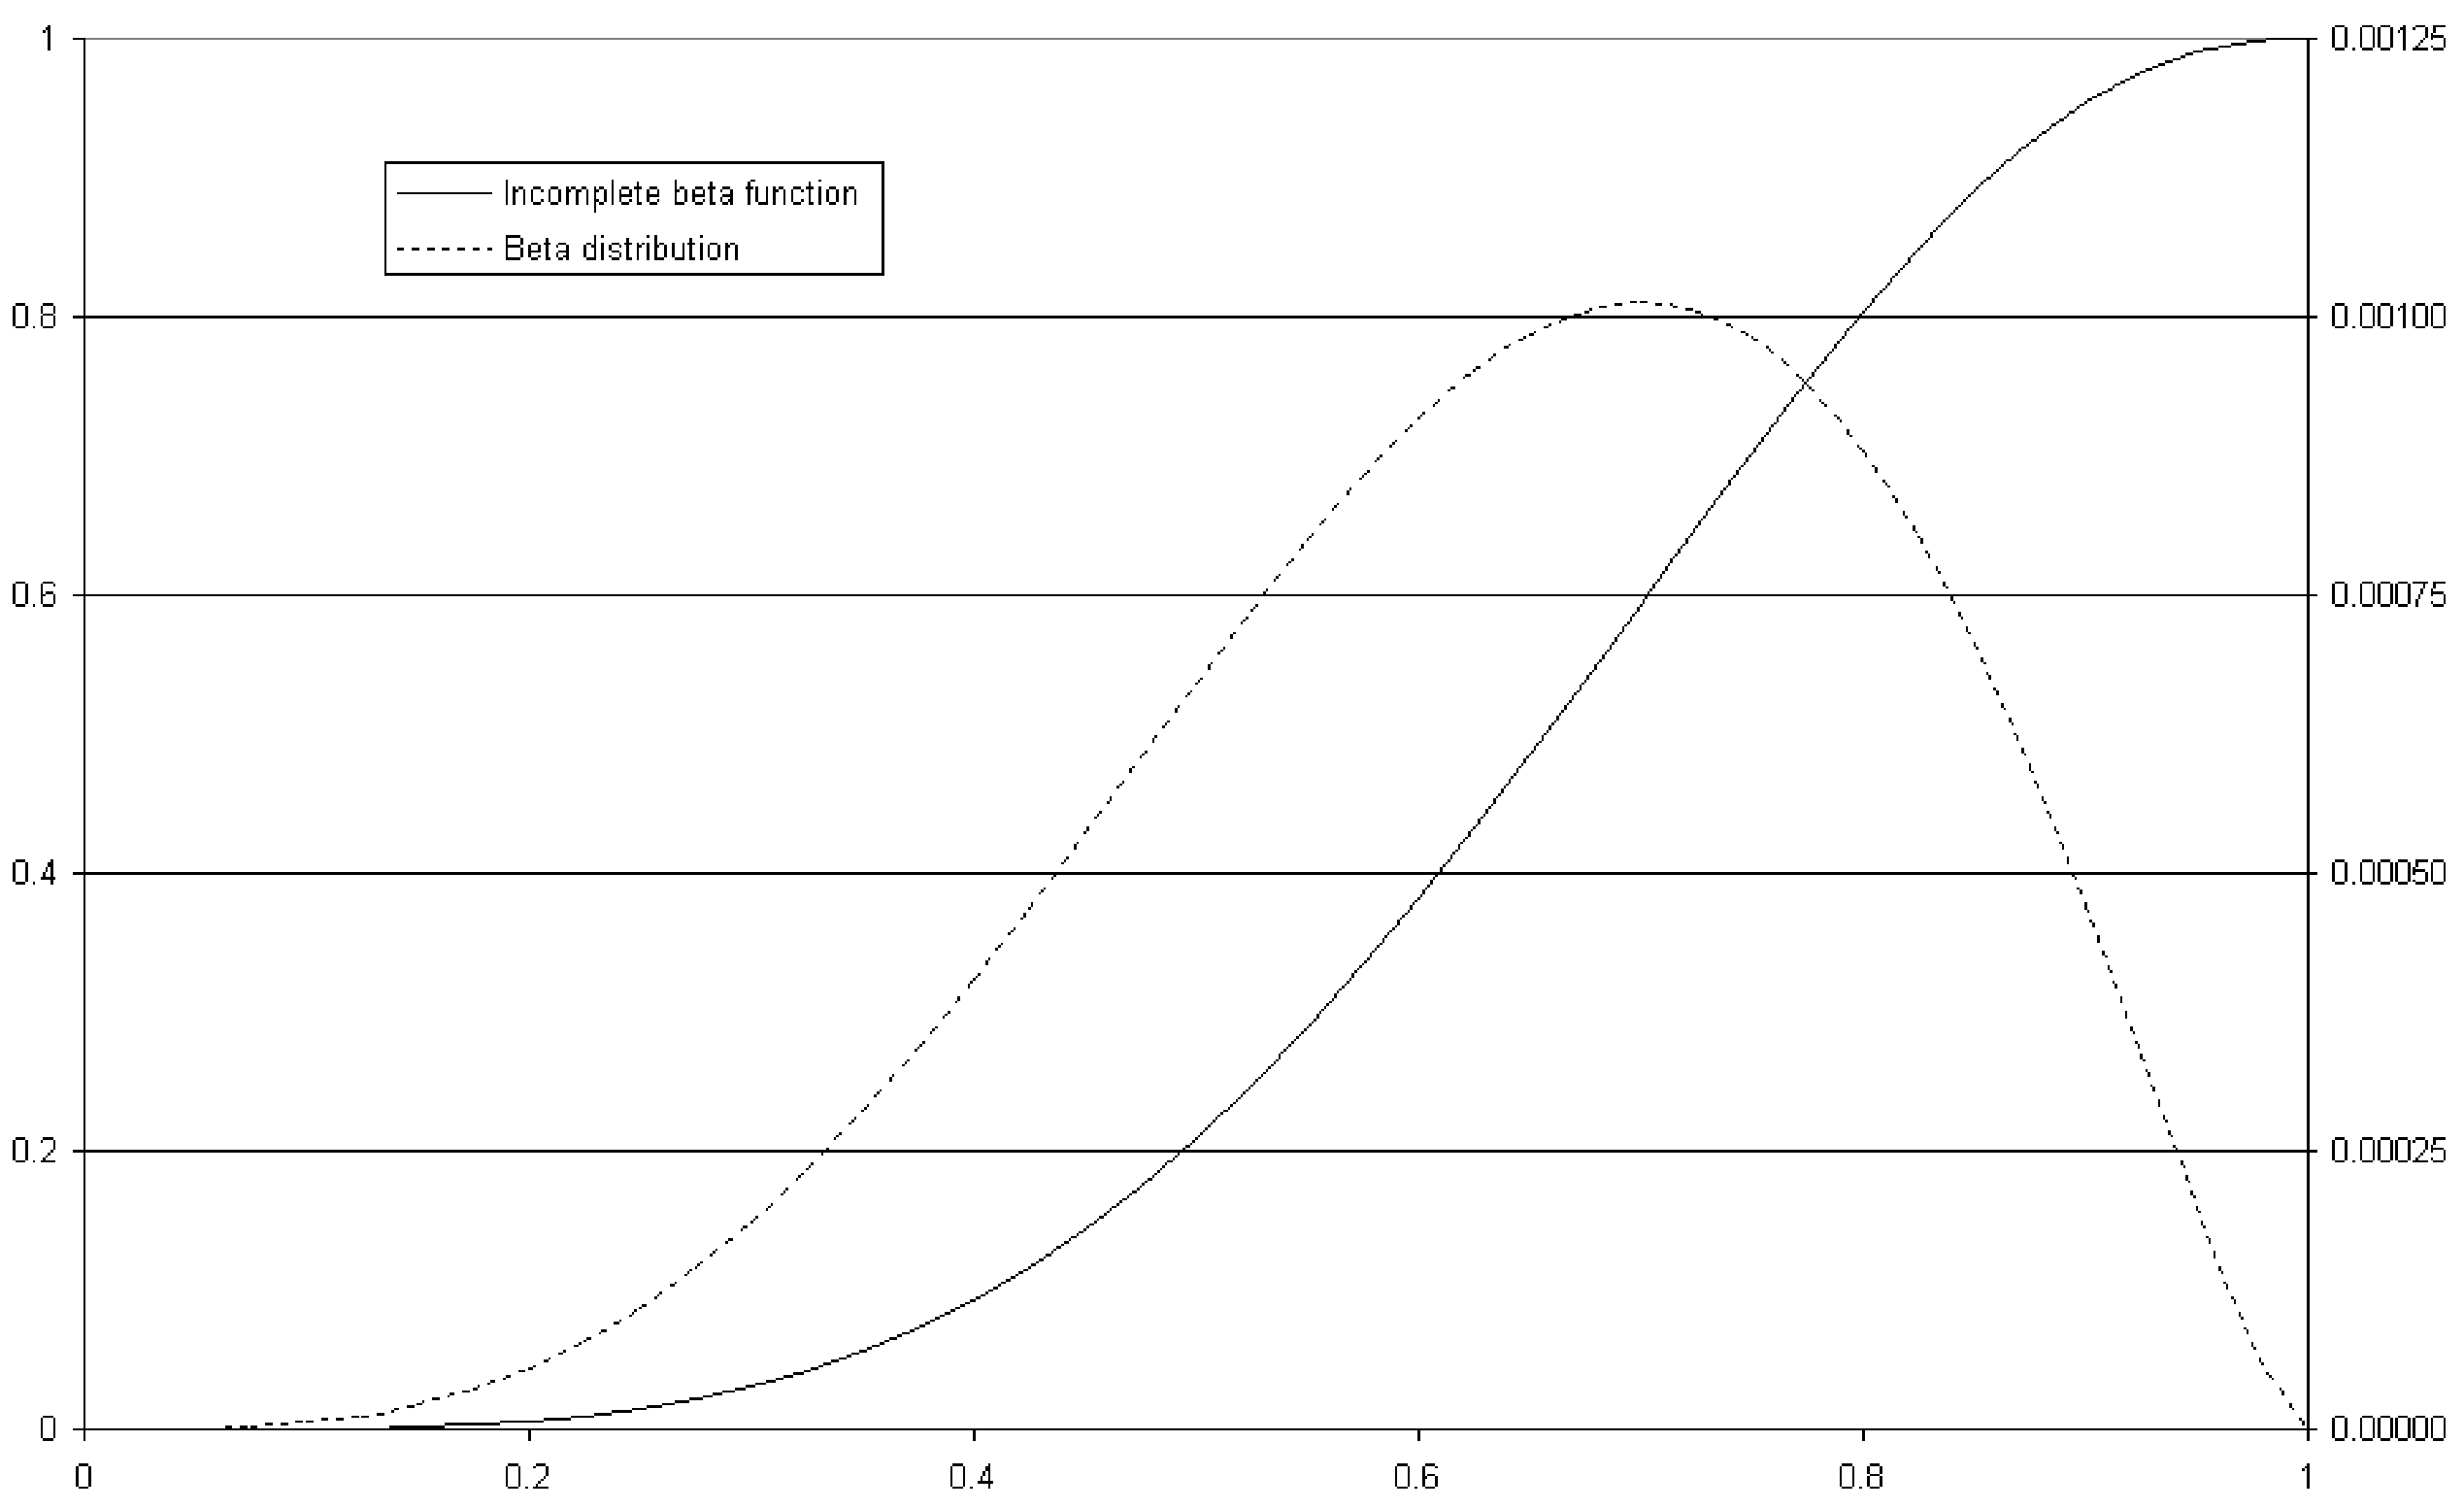
\includegraphics[width=10cm]{Figures/IncompleteBetaFunction}
\caption{The incomplete beta function and the beta distribution}\label{fig:incBetaFunction}
\end{figure}

\subsection{Mathematical definitions}
The incomplete beta function is defined over the interval
$\left[0,1\right]$ by the following integral:
\begin{equation}
\label{eq:incBetaFunction}
  B\left(x;\alpha_1,\alpha_2\right)={1\over B\left(\alpha_1,\alpha_2\right)}
  \int_0^x t^{\alpha_1-1}\left(1-t\right)^{\alpha_2-1}dt,
\end{equation}
where $B\left(\alpha_1,\alpha_2\right)$ is the beta function
defined in section \ref{sec:betafunc}. The function has two
parameters $\alpha_1$ and $\alpha_2$. By definition, the value of
the incomplete beta function is comprised between 0 and 1.

None of the series expansions of this integral have good numerical
convergence. There is, however, a continued fraction development
which converges over a sufficient range \cite{AbrSteg}:
\begin{equation}
\label{eq:incbeta}
  B\left(x;\alpha_1,\alpha_2\right)={x^{\alpha_1-1}\left(1-x\right)^{\alpha_2-1}\over
  \alpha_1 B\left(\alpha_1,\alpha_2\right)}
  {1\over F\left(x;\alpha_1,\alpha_2\right)},
\end{equation}
where
\begin{equation}
  F\left(x;\alpha_1,\alpha_2\right)=1+
  {a_1\over 1+}{a_2\over 1+}{a_3\over 1+}\cdots
\end{equation}
Using the notation introduced in section \ref{sec:contfractions}
we have:
\begin{equation}
\label{eq:incbetaterm}
  \left\{{
  \begin{array}{lcl}
    b_n & = & 1\mbox{\quad for $n=0,1,2,\ldots$} \\*[1ex]
    a_{2n} & = & {\displaystyle n\left(\alpha_2-n\right)x \over \displaystyle\left(\alpha_1+2n\right)
    \left(\alpha_1+2n-1\right)} \mbox{\quad for $n=1,2,\ldots$} \\*[3ex]
    a_{2n+1} & = & {\displaystyle\left(\alpha_1+n\right)\left(\alpha_1+\alpha_2+n\right)x \over \displaystyle\left(\alpha_1+2n\right)
    \left(\alpha_1+2n-1\right)} \mbox{\quad for $n=1,2,\ldots$}
  \end{array}
  }\right.
\end{equation}
The continued fraction in equation \ref{eq:incbeta} converges
rapidly for $x>{\alpha_1+1 \over
\alpha_1+\alpha_2+2}$\cite{Press}. To compute the incomplete beta
function over the complementary range, one uses the following
symmetry property of the function:
\begin{equation}
  B\left(x;\alpha_1,\alpha_2\right)=1-B\left(1-x;\alpha_2,\alpha_1\right)
\end{equation}
Since $1-x<{\alpha_2+1 \over \alpha_1+\alpha_2+2}$ if
$x<{\alpha_1+1 \over \alpha_1+\alpha_2+2}$, we can now compute the
function over the entire range.

To avoid a floating-point error when evaluating the leading factor
of equation \ref{eq:incbeta}, the values of the incomplete beta
function at $x=0$ --- which is 0 --- and at $x=1$ --- which is 1
--- must be returned separately.

\subsection{Incomplete Beta function --- Smalltalk  implementation}
%\marginpar{Figure \ref{fig:StSeriesClass} with the boxes {\bf IncompleteBetaFunction} and {\tt IncompleteBetaFractionTermServer} grayed.}
Listing \ref{lst:incbeta} shows the implementation of the
incomplete beta function in Smalltalk.

Two classes are needed to implement the incomplete beta function.
The class \code{PMIncompleteBetaFunction} is in charge of
computing the function itself. This class has the following
instance variables.
\begin{itemize}
\item \code{alpha1} contains the first function's parameter, i.e.
$\alpha_1$,
\item \code{alpha2} contains the second function's parameter, i.e.
$\alpha_2$,
\item \code{logNorm} used to cache the value of $\ln B\left(\alpha_1,\alpha_2\right)$ for efficiency purposes,
\item \code{fraction} contains the continued fraction associated to the
function $B\left(x;\alpha_1,\alpha_2\right)$,
\item \code{inverseFraction} contains the continued fraction associated to the
function $B\left(1-x;\alpha_2,\alpha_1\right)$.
\end{itemize}
Depending on the range of the argument, the class delegates the
rest of the computing to a continued fraction using the original
parameters or the reversed parameters if the symmetry relation
must be used. A term server class allows the computing of the
terms. Its code is shown in listing \ref{lst:incbetaterm}. The two
instance variables - \code{fraction} and \code{inverseFraction} -,
contain an instance of the term server, one for each permutation
of the parameters, thus preventing the unnecessary creation of new
instances of the term server at each evaluation. These instance
variables are assigned using lazy initialization.

\begin{listing}[label=lst:incbeta]{Smalltalk}
{Smalltalk implementation of the incomplete beta function}
Object subclass: #PMIncompleteBetaFunction
   instanceVariableNames: 'alpha1 alpha2 fraction inverseFraction logNorm'
   classVariableNames: ''
   package: 'Math-DistributionBeta'
\end{listing}

\begin{displaycode}{Smalltalk}
PMIncompleteBetaFunction class >> shape: aNumber1 shape: aNumber2
   ^self new initialize: aNumber1 shape: aNumber2
\end{displaycode}

\begin{displaycode}{Smalltalk}
PMIncompleteBetaFunction >>evaluateFraction: aNumber
    fraction isNil 
        ifTrue: 
            [ fraction := PMIncompleteBetaFractionTermServer new.
            fraction setParameter: alpha1 second: alpha2 ].
    fraction setArgument: aNumber.
    ^(PMContinuedFraction server: fraction)
        desiredPrecision: PMFloatingPointMachine new defaultNumericalPrecision;
        evaluate
\end{displaycode}

\begin{displaycode}{Smalltalk}
PMIncompleteBetaFunction >> evaluateInverseFraction: aNumber
    inverseFraction isNil 
        ifTrue: 
            [ inverseFraction := PMIncompleteBetaFractionTermServer new.
            inverseFraction setParameter: alpha2 second: alpha1 ].
    inverseFraction setArgument: (1 - aNumber).
    ^(PMContinuedFraction server: inverseFraction)
        desiredPrecision: PMFloatingPointMachine new defaultNumericalPrecision;
        evaluate
\end{displaycode}

\begin{displaycode}{Smalltalk}
PMIncompleteBetaFunction >> initialize: aNumber1 shape: aNumber2
    alpha1 := aNumber1.
    alpha2 := aNumber2.
    logNorm := ( alpha1 + alpha2) logGamma - alpha1 logGamma - alpha2 logGamma.
    ^ self
\end{displaycode}

\begin{displaycode}{Smalltalk}
PMIncompleteBetaFunction >> value: aNumber
    | norm |
    aNumber = 0
        ifTrue: [ ^ 0 ].
    aNumber = 1
        ifTrue: [ ^ 1 ].
    norm :=  (aNumber ln * alpha1 + ((1 - aNumber) ln * alpha2) + logNorm) exp.
    ^ (alpha1 + alpha2 + 2) * aNumber < (alpha1 + 1)
        ifTrue: [ norm / ( ( self evaluateFraction: aNumber) * alpha1)]
        ifFalse: [ 1 - ( norm / ( ( self evaluateInverseFraction: aNumber) * alpha2)) ]
\end{displaycode}

Listing \ref{lst:incbetaterm} shows the implementation of the term
server. It needs two instance variables to store the parameters
$\alpha_1$ and $\alpha_2$. Equation \ref{eq:incbetaterm} is
implemented by the methods \code{initialTerm} (for $n=0$) and \code{termsAt:} (for $n\ge 1$).

\begin{listing}[label=lst:incbetaterm]{Smalltalk}
{Smalltalk implementation of the term server for the incomplete beta function}
PMSeriesTermServer subclass: #PMIncompleteBetaFractionTermServer
   instanceVariableNames: 'alpha1 alpha2'
   classVariableNames: ''
   package: 'Math-DHB-Numerical'
\end{listing}

\begin{displaycode}{Smalltalk}
PMIncompleteBetaFractionTermServer >> initialTerm
    ^ 1
\end{displaycode}

\begin{displaycode}{Smalltalk}
PMIncompleteBetaFractionTermServer >> setParameter: aNumber1 second: aNumber2
    alpha1 := aNumber1.
    alpha2 := aNumber2
\end{displaycode}

PMIncompleteBetaFractionTermServer >> termsAt: anInteger
\begin{displaycode}{Smalltalk}
    | n n2 |
    n := anInteger // 2.
    n2 := 2 * n.
    ^Array with: ( n2 < anInteger 
        ifTrue: [ x negated * (alpha1 + n) * (alpha1 + alpha2 + n) 
                                / ((alpha1 + n2) * (alpha1 + 1 + n2))]
        ifFalse: [x * n * (alpha2 - n) / ((alpha1 + n2) * (alpha1 - 1 + n2)) ])
            with: 1
\end{displaycode}

An example of use of the incomplete beta function can be found in
sections \ref{sec:Ftest} and \ref{sec:ttest}.


%\ifx\wholebook\relax\else\end{document}\fi

%\ifx\wholebook\relax\else
%\documentclass[twoside]{book}
%\usepackage[active]{srcltx}
%\usepackage[LY1]{fontenc}
%\usepackage{url}
\makeatletter
\def\url@leostyle{%
  \@ifundefined{selectfont}{\def\UrlFont{\sf}}{\def\UrlFont{\sffamily}}}
\makeatother
% Now actually use the newly defined style.
\urlstyle{leo}

\usepackage{graphicx}
\def\etc{{\textit{etc}}}
\def\eg{{\textit{e.g.}}}
\def\ie{{\textit{i.e.}}}
\def\cf{{\textit{c.f.}}\ }
\def\erf{\mathop{\textrm{erf}}}
\def\sign{\mathop{\textrm{sign}}}
\def\prob{\mathop{\textrm{Prob}}}
\def\var{\mathop{\textrm{var}}}
\def\mod{\mathop{\textrm{mod}}}
\def\cor{\mathop{\textrm{cor}}}
\def\cov{\mathop{\textrm{cov}}}
\def\cl{\mathop{\textrm{CL}}}
\def\kg{\mathop{\textrm{Kg}}}
\def\patstyle#1{{\textsc #1}}
\def\th{^{\mathop{\textrm{th}}}}
%\def\st#1{^{\mathop{\rm #1}}}
\def\note#1{\begin{quote}{\textbf{Note:}} #1\end{quote}}
\def\braket#1{\left\langle #1\right\rangle}
\def\order#1{\let\o=#1$\mathcal{O}$\ifx\o 1$\left(n\right)$\else$\left(n^{#1}\right)$\fi}
%\newtheorem{privListing}{Listing}[chapter]
%\newenvironment{listing}{\vskip 3ex\hrule\vskip 1ex\begin{privListing}}{\end{privListing}\hrule\vskip 1ex}
\newtheorem{privExample}{Code example}[chapter]
\newenvironment{codeExample}{\begin{privExample}\begin{quote}\tt}{\end{quote}\end{privExample}}
\def\relboxl#1#2{\hbox to #1\hsize{#2\hfil}}
\def\relboxc#1#2{\hbox to #1\hsize{\hfil #2\hfil}}
\def\relboxr#1#2{\hbox to #1\hsize{\hfil #2}}
\def\transpose#1{\textbf{#1}^{\mathop\textrm{T}}}
\def\inverse#1{\textbf{#1}^{-1}}
%\def\tm{$^{\mathop{\rm TM}}$}
\def\tm{ }
\newenvironment{mainEquation}{\marginpar[\vspace{3 ex} Main
equation$\Rightarrow$]{\vspace{3 ex}$\Leftarrow$Main
equation}\begin{equation}}{\end{equation}}
\def\rubrique#1{\paragraph{#1}\hfil\par\noindent}

%\begin{document}
%\fi

\chapter{Linear algebra}
\label{ch:linearalgebra}
\begin{flushright}
{\textsl On ne trouve pas l'espace, il faut toujours le
construire.}\footnote{Space is not to be found; it must always be
constructed.}\\ Gaston Bachelard
\end{flushright}
\vspace{1 ex} Linear algebra concerns itself with the manipulation
of vectors and matrices. The concepts of linear algebra are not
difficult and linear algebra is usually taught in the first year
of university. Solving systems of linear equations are even taught
in high school. Of course, one must get used to the book keeping
of the indices. The concise notation introduced in linear algebra
for vector and matrix operations allows expressing difficult
problems in a few short equations. This notation can be directly
adapted to object oriented programming.

Figure \ref{fig:linearalgebraclasses} shows the classes described
in this chapter.
\begin{figure}
\centering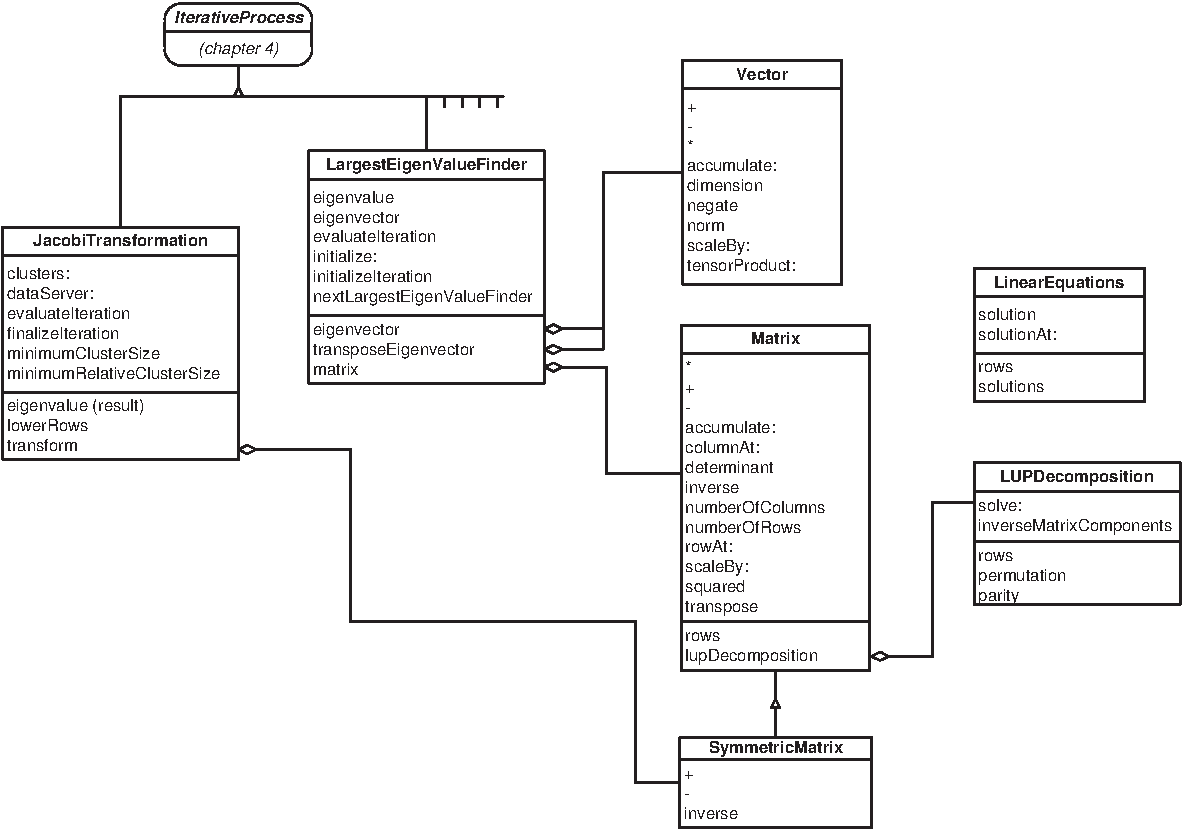
\includegraphics[width=11cm]{Figures/LinearAlgebraClasses}
\caption{Linear algebra classes}\label{fig:linearalgebraclasses}
\end{figure}
Like chapter \ref{ch:function}, this chapter discusses some
fundamental concepts and operations that shall be used throughout
the rest of the book. It might appear austere to many readers
because, unlike the preceding chapters, it does not contains
concrete examples. However, the reader will find example of use of
linear algebra in nearly all remaining chapters of this book.

The chapter begins with a reminder of operations defined on
vectors and matrices. Then, two methods for solving systems of
linear equations are discussed. This leads to the important
concept of matrix inversion. Finally the chapter closes of the
problem of finding eigenvalues and eigenvectors.

\section{Vectors and matrices}
\label{sec:linearalgebra} Linear algebra concerns itself with
vectors in multidimensional spaces and the properties of
operations on these vectors. It is a remarkable fact that such
properties can be studied without explicit specification of the
space dimension\footnote{In fact, most mathematical properties
discussed in this chapter are valid for space with an infinite
number of dimensions (Hilbert spaces).}.

A vector is an object in a multidimensional space. It is
represented by its components measured on a reference system. A
reference system is a series of vectors from which the entire
space can be generated. A commonly used mathematical notation for
a vector is a lower case bold letter, ${\textbf{v}}$ for example. If
the set of vectors ${\textbf{u}}_1,\ldots,{\textbf{u}}_n$ is a reference
system for a space with $n$ dimension, then any vector of the
space can be written as:
\begin{equation}
\label{eq:vectordef}
  {\textbf{v}} = v_1{\textbf{u}}_1+\cdots+v_n{\textbf{u}}_n,
\end{equation}
where $v_1,\ldots,v_n$ are real numbers in the case of a real
space or complex numbers in a complex space. The numbers
$v_1,\ldots v_n$ are called the components of the vector.

A matrix is a linear operator over vectors from one space to
vectors in another space not necessarily of the same dimension.
This means that the application of a matrix on a vector is another
vector. To explain what {\textsl linear} means, we must quickly
introduce some notation.

A matrix is commonly represented with an upper case bold letter,
${\textbf{M}}$ for example. The application of the matrix ${\textbf{M}}$ on
the vector ${\textbf{M}}$ is denoted by ${\textbf{M}}\cdot{\textbf{v}}$. The fact
that a matrix is a linear operator means that
\begin{equation}
{\textbf{M}}\cdot\left(\alpha{\textbf{u}}+\beta{\textbf{v}}\right)=\alpha{\textbf
{M}}\cdot{\textbf{u}}+\beta{\textbf{M}}\cdot{\textbf{v}},
\end{equation}
for any matrix ${\textbf{M}}$, any vectors ${\textbf{u}}$ and ${\textbf{v}}$, any
numbers $\alpha$ and $\beta$.

Matrices are usually represented using a table of numbers. In
general, the number of rows and the number of columns are not the
same. A square matrix is a matrix having the same number of rows
and columns. A square matrix maps a vector onto another vector of
the same space.

Vectors and matrices have an infinite number of representations
depending on the choice of reference system. Some properties of
matrices are independent from the reference system. Very often the
reference system is not specified explicitly. For example, the
vector ${\textbf{v}}$ of equation \ref{eq:vectordef} is represented by
the array of numbers $\left( v_1v_2\cdots v_n\right)$ where $n$ is
the dimension of the vector. Writing the components of a vector
within parentheses is customary. Similarly a matrix is represented
with a table of numbers called the components of the matrix; the
table is also enclosed within parentheses. For example, the $n$ by
$m$ matrix ${\textbf{A}}$ is represented by:
\begin{equation}
  {\textbf{A}}=\pmatrix{a_{11}& a_{12}&\ldots& a_{1n}\cr
  a_{21}& a_{22}&\ldots& a_{2n}\cr
  \vdots&\vdots&\ddots&\vdots\cr
  a_{m1}& a_{m2}&\ldots& a_{mn}\cr}.
\end{equation}
The components can be real or complex numbers. In this book we
shall deal only with vectors and matrices having real components.

For simplicity a matrix can also be written with matrix
components. That is, the $n$ by $m$ matrix ${\textbf{A}}$ can be
written in the following form:
\begin{equation}
\label{eq:matrixcomp}
  {\textbf{A}}=\pmatrix{{\textbf{B}}&{\textbf{C}}\cr{\textbf{D}}&{\textbf{E}}\cr},
\end{equation}
where $\textbf{B}$, ${\textbf{C}}$, ${\textbf{D}}$ and ${\textbf{E}}$ are all
matrices of lower dimensions. Let ${\textbf{B}}$ be a $p$ by $q$
matrix. Then, ${\textbf{C}}$ is a $p$ by $m-q$ matrix, ${\textbf{D}}$ is a
$n-p$ by $q$ matrix and ${\textbf{E}}$ is a $n-p$ by $m-q$ matrix.

Using this notation one can carry all conventional matrix
operations using formulas similar to those written with the
ordinary number components. There is, however, one notable
exception: the order of the products must be preserved since
matrix multiplication is not commutative. For example, the product
between two matrices expressed as matrix components can be carried
out as:
\begin{equation}
\label{eq:matrixcompmult}
  \pmatrix{\textbf{B}_1&\textbf{C}_1\cr\textbf{D}_1&\textbf{E}_1\cr}\cdot
  \pmatrix{\textbf{B}_2&\textbf{C}_2\cr\textbf{D}_2&\textbf{E}_2x\cr}=
  \pmatrix{\textbf{B}_1\cdot\textbf{B}_2+\textbf{C}_1\cdot\textbf{D}_2&
  \textbf{B}_1\cdot\textbf{C}_2+\textbf{C}_1\cdot\textbf{E}_2\cr
  \textbf{D}_1\cdot\textbf{B}_2+\textbf{E}_1\cdot\textbf{D}_2&
  \textbf{D}_1\cdot\textbf{C}_2+\textbf{E}_1\cdot\textbf{E}_2\cr},
\end{equation}
In equation \ref{eq:matrixcompmult} the dimension of the
respective matrix components must permit the corresponding
product.
For example the number of rows of the matrices $\textbf{B}_1$ and $\textbf{C}_1$ must be equal to the number of columns of the matrices $\textbf{B}_2$ and $\textbf{C}_2$ respectively.

Common operations defined on vectors and matrices are summarized
below. In each equation, the left-hand side shows the vector
notation and the right-hand side shows the expression for
coordinates and components.

\vskip 2ex\noindent The sum of two vectors of dimension $n$ is a
vector of dimension $n$:
\begin{equation}
\label{eq:vectorsum}
\begin{tabular}{ccl}
\relboxc{0.27}{$\textbf{w}=\textbf{u}+{\textbf
v}$}&\relboxc{0.27}{$w_i=u_i+v_i$}&\relboxl{0.27}{for
$i=1,\ldots,n$}
\end{tabular}
\end{equation}
The product of a vector of dimension $n$ by a number $\alpha$ is a
vector of dimension $n$:
\begin{equation}
\begin{tabular}{ccl}
\relboxc{0.27}{$\textbf{w}=\alpha\textbf{v}$}&\relboxc{0.27}{$w_i=\alpha
v_i$}&\relboxl{0.27}{for $i=1,\ldots,n$}
\end{tabular}
\end{equation}
The scalar product of two vectors of dimension $n$ is a number:
\begin{equation}
\begin{tabular}{ccl} \relboxc{0.27}{$s=\textbf{u}\cdot{\textbf
v}$}&\relboxc{0.27}{$\displaystyle s=\sum_{i=1}^n u_i
v_i$}&\relboxc{0.27}{ }
\end{tabular}
\end{equation}
The norm of a vector is denoted $\left|\textbf{v}\right|$. The norm
is the square root of the scalar product with itself.
\begin{equation}
\begin{tabular}{ccl} \relboxc{0.27}{$\left|\textbf{v}\right|=\sqrt{\textbf{v}\cdot{\textbf
v}}$}&\relboxc{0.27}{$\left|{\textbf
v}\right|=\sqrt{\displaystyle\sum_{i=1}^n v_i
v_i}$}&\relboxc{0.27}{ }
\end{tabular}
\end{equation}
The tensor product of two vectors of respective dimensions $n$ and
$m$ is an $n$ by $m$ matrix:
\begin{equation}
\begin{tabular}{ccl}
 \relboxc{0.27}{$\textbf{T}=\textbf{u}\otimes\textbf{v}$}&\relboxc{0.27}{$T_{ij}=u_i v_j$}&\relboxl{0.27}{for
$i=1,\ldots,n$}\\&&\relboxl{0.27}{and $j=1,\ldots,m$}
\end{tabular}
\end{equation}
The sum of two matrices of same dimensions is a matrix of same
dimensions:
\begin{equation}
\begin{tabular}{ccc}
  \relboxc{0.27}{$\textbf{C}=\textbf{A}+\textbf{B}$}&\relboxc{0.27}{$c_{ij}=a_{ij}+b_{ij}$}&\relboxl{0.27}{for $i=1,\ldots,n$}\\
  &&\relboxl{0.27}{and $j=1,\ldots,m$}\\
\end{tabular}
\end{equation}
The product of a matrix by a number $\alpha$ is a matrix of same
dimensions:
\begin{equation}
\begin{tabular}{ccc}
  \relboxc{0.27}{$\textbf{B}=\alpha\textbf{A}$}&\relboxc{0.27}{$b_{ij}=\alpha a_{ij}$}&\relboxl{0.27}{for $i=1,\ldots,n$}\\
  &&\relboxl{0.27}{and $j=1,\ldots,m$}\\
\end{tabular}
\end{equation}
The transpose of a $n$ by $m$ matrix is a $m$ by $n$ matrix:
\begin{equation}
\begin{tabular}{ccc}
  \relboxc{0.27}{$\textbf{B}=\textbf{A}^{\mathop{\textrm{T}}}$}&\relboxc{0.27}{$b_{ij}=a_{ji}$}&\relboxl{0.27}{for $i=1,\ldots,n$}\\
  &&\relboxl{0.27}{and $j=1,\ldots,m$}\\
\end{tabular}
\end{equation}
The product of a $n$ by $m$ matrix with a vector of dimension $n$
is a vector of dimension $m$:
\begin{equation}
\begin{tabular}{ccc}
  \relboxc{0.27}{$\textbf{u}=\textbf{A}\cdot\textbf{v}$}&\relboxc{0.27}{$u_i=\displaystyle\sum_{i=1}^n a_{ij}v_i$}&\relboxl{0.27}{for $i=1,\ldots,m$}\\
\end{tabular}
\end{equation}
The transposed product of a vector of dimension $m$ by a $n$ by
$m$ matrix is a vector of dimension $n$:
\begin{equation}
\begin{tabular}{ccc}
  \relboxc{0.27}{$\textbf{u}=\textbf{v}\cdot\textbf{A}$}&\relboxc{0.27}{$u_i=\displaystyle\sum_{i=1}^m a_{ji}v_i$}&\relboxl{0.27}{for $i=1,\ldots,m$}\\
\end{tabular}
\end{equation}
The product of a $n$ by $p$ matrix with a $p$ by $m$ matrix is a
$n$ by $m$ matrix:
\begin{equation}
\label{eq:matrixproduct}
\begin{tabular}{ccc}
  \relboxc{0.27}{$\textbf{C}=\textbf{A}\cdot\textbf{B}$}&\relboxc{0.27}{$c_{ij}=\displaystyle\sum_{k=1}^p a_{ik}a_{kj}$}&\relboxl{0.27}{for $i=1,\ldots,m$}\\
  &&\relboxl{0.27}{$j=1,\ldots,m$}\\
\end{tabular}
\end{equation}
There are of course other operations (the outer product for
example) but they will not be used in this book.

To conclude this quick introduction, let us mention matrices with
special properties.

A square matrix is a matrix which has the same number of rows and
columns. To shorten sentences, we shall speak of a square matrix
of dimension $n$ instead of a $n$ by $n$ matrix.

An identity matrix $\textbf{I}$ is a matrix such that
\begin{equation}
  \textbf{I}\cdot\textbf{v}=\textbf{v}
\end{equation}
for any vector $\textbf{v}$. This implies that the identity matrix is
a square matrix. the representation of the identity matrix
contains 1 in the diagonal and 0 off the diagonal in any system of
reference. For any square matrix $\textbf{A}$ we have:
\begin{equation}
  \textbf{I}\cdot\textbf{A}=\textbf{A}\cdot\textbf{I}=\textbf{A}
\end{equation}

One important property for the algorithms discussed in this book
is symmetry. A symmetrical matrix is a matrix such that ${\textbf
A}^{\mathop{\textrm{T}}}={\textbf{A}}$. In any system of reference the
components of a symmetric matrix have the following property:
\begin{equation}
  a_{ij}=a_{ji}, \mbox{\quad for all $i$ and $j$.}
\end{equation}
The sum and product of two symmetric matrices is a symmetric
matrix. The matrix ${\textbf{A}}^{\mathop{\textrm{T}}}\cdot{\textbf{A}}$ is a
symmetric matrix for any matrix ${\textbf{A}}$. If the matrix ${\textbf{A}}$
represented in equation \ref{eq:matrixcomp} is symmetric, we have
${\textbf{D}}={\textbf{C}}^{\mathop{\textrm{T}}}$.

\subsection{Vector and matrix implementation}
\label{sec:slinearalgebra}
%\marginpar{Figure\ref{fig:linearalgebraclasses} with the box \textbf{Vector} and \textbf{Matrix} grayed.}
Listings \ref{lst:vector} and \ref{lst:matrix} show respectively the implementation of vectors and matrices.
A special implementation for symmetric matrices is shown in listing \ref{lst:symmatrix}.

The public interface is designed as to map itself as close as
possible to the mathematical definitions. Here are some example of
code using operations between vectors and matrices:
\begin{displaycode}{Smalltalk}
| u v w a b c |
u := #(1 2 3) asPMVector.
v := #(3 4 5) asPMVector.
a := PMMatrix rows: #((1 0 1) (-1 -2 3)).
b := PMMatrix rows: #((1 2 3) (-2 1 7) (5 6 7)).
w := 4 * u + (3 * v).
c := a * b.
v := a * u.
w := c transpose * v.
w := v * c
\end{displaycode}
In the first two lines after the declarative statement, the
vectors ${\textbf{u}}$ and ${\textbf{v}}$ are defined from their component
array using the creator method \code{asPMVector}.
They are 3-dimensional vectors. The matrices ${\textbf{a}}$ and ${\textbf{b}}$ are
created by supplying the components to the class creation method \code{rows:}. The matrix $\textbf{a}$ is a 2 by 3 matrix, whereas the
matrix $\textbf{b}$ is a square matrix of dimension 3. In all cases
the variable \code{w} is assigned to a vector and the variable \code{c} is assigned to a matrix. First, the vector $\textbf{w}$ is
assigned to a linear combination of the vectors $\textbf{u}$ and
$\textbf{v}$. Apart from the parentheses required for the second
product, the expression is identical to what one would write in
mathematics (compare this expression with equation
\ref{eq:vectordef}).

Next the matrix $\textbf{c}$ is defined as the product of the
matrices $\textbf{a}$ and $\textbf{b}$ in this order. It is a direct
transcription of the left part of equation \ref{eq:matrixproduct}
up to the case of the operands.

The next assignment redefines the vector $\textbf{v}$ as the product
of the matrix $\textbf{A}$ with the vector $\textbf{u}$. It is now a
2-dimensional vector. Here again the correspondence between the
Pharo and the mathematical expression is direct.

The last two lines compute the vector $\textbf{w}$ as the transpose
product with the matrix $\textbf{a}$. The result of both line is the
same\footnote{\label{ft:covariant}There is a subtle difference
between regular vectors and transposed vectors, which is
overlooked by our choice of implementation, however. Transposed
vectors or covariant vectors as they are called in differential
geometry should be implemented in a proper class. This extension
is left as an exercise to the reader.}. The first line makes the
transposition of the matrix $\textbf{a}$ explicit, whereas the second
line used the implicit definition of the transpose product. The
second line is faster than the previous one since no memory
assignment is required for the temporary storage of the transpose
matrix.

The use of other methods corresponding to the operations defined
in equations \ref{eq:vectorsum} to \ref{eq:matrixproduct} are left
as an exercise to the reader.

\rubrique{Implementation} A vector is akin to an instance of the
Pharo class \code{Array}, for which mathematical operations
have been defined.
Thus, a vector in Pharo can be implemented directly as a subclass of the class \code{Array}.
A matrix is an object whose instance variable is an array of vectors.

The operations described in the preceding section can be assigned
to the corresponding natural operators. The multiplication,
however, can involve several types of operands. It can be applied
between
\begin{enumerate}
  \item a vector and a number,
  \item a matrix and a number or
  \item a vector and a matrix.
\end{enumerate}
Thus, the multiplication will be implemented using double
dispatching as explained in section \ref{sec:polymath} for
operations between polynomials. Double dispatching is described in
appendix (\cf section \ref{sec:doubledisp}).

The method \code{asPMVector} is defined for compatibility with a
similar method defined in the class \code{Collection} to construct a
vector out of any collection object.

The method \code{tensorProduct} returns an instance of a symmetric
matrix.
This class is defined in listing \ref{ls:symmatrix}.

The method \code{accumulate} is meant to be used when there is a
need to add several vectors.
Indeed the following code
\begin{displaycode}{Smalltalk}
| a b c d e |
a := #(1 2 3 4 5) asPMVector.
b := #(2 3 4 5 6) asPMVector.
c := #(3 4 5 6 7) asPMVector.
d := #(4 5 6 7 8) asPMVector.
e := a+b+c+d.
\end{displaycode}
creates a lots of short-lived vectors, namely one
for each addition.
Using the method \code{accumulate} reduces the memory allocation:
\begin{displaycode}{Smalltalk}
| a b c d e |
a := #(1 2 3 4 5) asPMVector.
b := #(2 3 4 5 6) asPMVector.
c := #(3 4 5 6 7) asPMVector.
d := #(4 5 6 7 8) asPMVector.
e := a copy.
e accumulate: b; accumulate: c; accumulate: d.
\end{displaycode}

If vectors of large dimension are used, using accumulation instead
of addition can make a big difference in performance since many
large short-lived objects put a heavy toll of the garbage
collector.

\begin{listing}[label=ls:vector]{Smalltalk}
{Vector class in Pharo}
Array variableSubclass: #PMVector
   instanceVariableNames: ''
   classVariableNames: ''
   package: 'Math-Core'
\end{listing}

\begin{displaycode}{Smalltalk}
PMVector >> * aNumberOrMatrixOrVector
    ^aNumberOrMatrixOrVector productWithVector: self
\end{displaycode}

\begin{displaycode}{Smalltalk}
PMVector >> + aVector
    | answer n |
    answer := self class new: self size.
    n := 0.
    self with: aVector do:
        [ :a :b | 
          n := n + 1. 
          answer at: n put: ( a + b).
        ].
    ^answer
\end{displaycode}

\begin{displaycode}{Smalltalk}
PMVector >> - aVector
    | answer n |
    answer := self class new: self size.
    n := 0.
    self with: aVector do:
        [ :a :b | 
          n := n + 1. 
          answer at: n put: ( a - b).
        ].
    ^answer
\end{displaycode}

\begin{displaycode}{Smalltalk}
PMVector >> accumulate: aVectorOrAnArray
    1 to: self size do: [ :n | self at: n put: ( ( self at: n) + ( 
                                            aVectorOrAnArray at: n))].
\end{displaycode}

\begin{displaycode}{Smalltalk}
PMVector >> accumulateNegated: aVectorOrAnArray
    1 to: self size do: [ :n | self at: n put: ( ( self at: n) - ( 
                                            aVectorOrAnArray at: n))].
\end{displaycode}

\begin{displaycode}{Smalltalk}
PMVector >> asVector
    ^ self
\end{displaycode}

\begin{displaycode}{Smalltalk}
PMVector >> dimension
    ^ self size
\end{displaycode}

\begin{displaycode}{Smalltalk}
PMVector >> negate
    1 to: self size do: [ :n | self at: n put: (self at: n) negated].
\end{displaycode}

\begin{displaycode}{Smalltalk}
PMVector >> norm
    ^ (self * self) sqrt
\end{displaycode}

\begin{displaycode}{Smalltalk}
PMVector >> normalized
    ^ (1 / self norm) * self
\end{displaycode}

\begin{displaycode}{Smalltalk}
PMVector >> productWithMatrix: aMatrix
    ^ aMatrix rowsCollect: [ :each | each * self ]
\end{displaycode}

\begin{displaycode}{Smalltalk}
PMVector >> productWithVector: aVector
    | n |
    n := 0.
    ^self inject: 0
            into: [ :sum :each | n := n + 1. (aVector at: n) * each + 
                                                                  sum ]
\end{displaycode}

\begin{displaycode}{Smalltalk}
PMVector >> scaleBy: aNumber
    1 to: self size do: [ :n | self at: n put: ( ( self at: n) * 
                                                            aNumber) ].
\end{displaycode}

\begin{displaycode}{Smalltalk}
PMVector >> tensorProduct: aVector
    self dimension = aVector dimension
        ifFalse:[ ^self error: 'Vector dimensions mismatch to build 
                                                     tensor product'].
    ^PMSymmetricMatrix rows: ( self collect: [ :a | aVector collect: 
                                                       [ :b | a * b]])
\end{displaycode}

\noindent The class \code{PMMatrix} has two instance variables:
\begin{itemize}
\item \code{rows} an array of vectors, each representing a
row of the matrix and
\item \code{lupDecomposition} a pointer to an object of the class \code{PMLUPDecomposition} containing the LUP decomposition of the matrix if already computed.
LUP decomposition is discussed in
section \ref{sec:lup}.
\end{itemize}
This implementation reuses the vector implementation of the vector
scalar product to make the code as compact as possible.
The iterator methods \code{columnsCollect:}, \code{columnsDo:}, \code{rowsCollect:} and \code{rowsDo:} are designed to limit the need for index management to these methods only.

An attentive reader will have noticed that the iterator methods
\code{rowsDo:} and \code{rowsCollect:} present a potential breach of
encapsulation. Indeed, the following expression
\begin{quote}
\begin{verbatim}
 aMatrix rowsDo:[ :each | each at: 1 put: 0]
\end{verbatim}
\end{quote}
changes the matrix representation outside of the normal way.
Similarly, the expression
\begin{quote}
\begin{verbatim}
 aMatrix rowsCollect:[ :each | each]
\end{verbatim}
\end{quote}
gives direct access to the matrix's internal representation.

The method \code{square} implements the product of the transpose of
a matrix with itself. This construct is used in several algorithms
presented in this book.

\begin{quotation}
\noindent {\textbf{Note:}} The presented matrix implementation is
straightforward. Depending on the problem to solve, however, it is
not the most efficient one. Each multiplication allocates a lot of
memory. If the problem is such that one can allocate memory once
for all, more efficient methods can be designed.
\end{quotation}

The implementation of matrix operations --- addition, subtraction,
product --- uses double or multiple dispatching to determine
whether or not the result is a symmetric matrix. Double and
multiple dispatching are explained in sections
\ref{sec:doubledisp} and \ref{sec:multipledisp}. The reader who is
not familiar with multiple dispatching should trace down a few
examples between simple matrices using the debugger.


\begin{listing}[label=lst:matrix]{Smalltalk}
{Matrix classes}
%$$\halign{ #\hfil&\quad#\hfil\cr {\sl Class}& {\Large\bf DhbMatrix}\cr
{\sl Subclass of }&{\tt Object}\cr\noalign{\vskip 1ex}

{\sl Instance variable names:}&\parbox[t]{4 in}{\tt  rows lupDecomposition }\cr\noalign{\vskip 1ex}}$$


Class methods
{\parskip 1ex\par\noindent}
{\bf new:} {\tt anInteger}
\begin{verbatim}
    ^ self new initialize: anInteger
\end{verbatim}
{\bf rows:} {\tt anArrayOrVector}
\begin{verbatim}
    ^ self new initializeRows: anArrayOrVector
\end{verbatim}

Instance methods
{\parskip 1ex\par\noindent}
{\bf *} {\tt aNumberOrMatrixOrVector}
\begin{verbatim}
    ^ aNumberOrMatrixOrVector productWithMatrix: self
\end{verbatim}
{\bf +} {\tt aMatrix}
\begin{verbatim}
    ^ aMatrix addWithRegularMatrix: self
\end{verbatim}
{\bf -} {\tt aMatrix}
\begin{verbatim}
    ^ aMatrix subtractWithRegularMatrix: self
\end{verbatim}
{\bf accumulate:} {\tt aMatrix}
\begin{verbatim}
    | n |
    n := 0.
    self rowsCollect: [ :each | n := n + 1. each accumulate: ( 
                                                    aMatrix rowAt: n)]
\end{verbatim}
{\bf accumulateNegated:} {\tt aMatrix}
\begin{verbatim}
    | n |
    n := 0.
    self rowsCollect: [ :each | n := n + 1. each accumulateNegated: ( 
                                                    aMatrix rowAt: n)]
\end{verbatim}
{\bf addWithMatrix:} {\tt aMatrix} {\bf class:} {\tt aMatrixClass}
\begin{verbatim}
    | n |
    n := 0.
    ^ aMatrixClass rows: ( self rowsCollect: [ :each | n := n + 1. 
                                          each + ( aMatrix rowAt: n)])
\end{verbatim}
{\bf addWithRegularMatrix:} {\tt aMatrix}
\begin{verbatim}
    ^ aMatrix addWithMatrix: self class: aMatrix class
\end{verbatim}
{\bf addWithSymmetricMatrix:} {\tt aMatrix}
\begin{verbatim}
    ^ aMatrix addWithMatrix: self class: self class
\end{verbatim}
{\bf asSymmetricMatrix}
\begin{verbatim}
    ^ DhbSymmetricMatrix rows: rows
\end{verbatim}
{\bf columnAt:} {\tt anInteger}
\begin{verbatim}
    ^ rows collect: [ :each | each at: anInteger]
\end{verbatim}
{\bf columnsCollect:} {\tt aBlock}
\begin{verbatim}
    | n |
    n := 0.
    ^rows last collect: [ :each | n := n + 1. aBlock value: ( self 
                                                         columnAt: n)]
\end{verbatim}
{\bf columnsDo:} {\tt aBlock}
\begin{verbatim}
    | n |
    n := 0.
    ^ rows last do: [ :each | n := n + 1. aBlock value: ( self 
                                                         columnAt: n)]
\end{verbatim}
{\bf initialize:} {\tt anInteger}
\begin{verbatim}
    rows := ( 1 to: anInteger) asVector collect: [ :each | DhbVector 
                                                      new: anInteger].
\end{verbatim}
{\bf initializeRows:} {\tt anArrayOrVector}
\begin{verbatim}
    rows := anArrayOrVector asVector collect: [ :each | each 
                                                            asVector].
\end{verbatim}
{\bf isSquare}
\begin{verbatim}
    ^ rows size = rows last size
\end{verbatim}
{\bf isSymmetric}
\begin{verbatim}
    ^ false
\end{verbatim}
{\bf lupDecomposition}
\begin{verbatim}
    lupDecomposition isNil
        ifTrue: [ lupDecomposition :=DhbLUPDecomposition equations: 
                                                                rows].
    ^ lupDecomposition
\end{verbatim}
{\bf negate}
\begin{verbatim}
    rows do: [ :each |each negate].
\end{verbatim}
{\bf numberOfColumns}
\begin{verbatim}
    ^ rows last size
\end{verbatim}
{\bf numberOfRows}
\begin{verbatim}
    ^ rows size
\end{verbatim}
{\bf printOn:} {\tt aStream}
\begin{verbatim}
    | first |
    first := true.
    rows do: 
        [ :each |
          first ifTrue: [ first := false]
                 ifFalse:[ aStream cr].
          each printOn: aStream.
        ].
\end{verbatim}
{\bf productWithMatrix:} {\tt aMatrix}
\begin{verbatim}
    ^ self productWithMatrixFinal: aMatrix
\end{verbatim}
{\bf productWithMatrixFinal:} {\tt aMatrix}
\begin{verbatim}
    ^ self class rows: ( aMatrix rowsCollect: [ :row | self 
                                 columnsCollect: [ :col | row * col]])
\end{verbatim}
{\bf productWithSymmetricMatrix:} {\tt aSymmetricMatrix}
\begin{verbatim}
    ^ self class rows: ( self rowsCollect: [ :row | aSymmetricMatrix 
                                 columnsCollect: [ :col | row * col]])
\end{verbatim}
{\bf productWithTransposeMatrix:} {\tt aMatrix}
\begin{verbatim}
    ^ self class rows: ( self rowsCollect: [ :row | aMatrix 
                                    rowsCollect: [ :col | row * col]])
\end{verbatim}
{\bf productWithVector:} {\tt aVector}
\begin{verbatim}
    ^ self columnsCollect: [ :each | each * aVector]
\end{verbatim}
{\bf rowAt:} {\tt anInteger}
\begin{verbatim}
    ^ rows at: anInteger
\end{verbatim}
{\bf rowsCollect:} {\tt aBlock}
\begin{verbatim}
    ^ rows collect: aBlock
\end{verbatim}
{\bf rowsDo:} {\tt aBlock}
\begin{verbatim}
    ^ rows do: aBlock
\end{verbatim}
{\bf scaleBy:} {\tt aNumber}
\begin{verbatim}
    rows do: [ :each | each scaleBy: aNumber].
\end{verbatim}
{\bf squared}
\begin{verbatim}
    ^ DhbSymmetricMatrix rows: ( self columnsCollect: [ :col | self 
                               columnsCollect: [ :colT | col * colT]])
\end{verbatim}
{\bf subtractWithMatrix:} {\tt aMatrix} {\bf class:} {\tt aMatrixClass}
\begin{verbatim}
    | n |
    n := 0.
    ^ aMatrixClass rows: ( self rowsCollect: [ :each | n := n + 1. 
                                          each - ( aMatrix rowAt: n)])
\end{verbatim}
{\bf subtractWithRegularMatrix:} {\tt aMatrix}
\begin{verbatim}
    ^ aMatrix subtractWithMatrix: self class: aMatrix class
\end{verbatim}
{\bf subtractWithSymmetricMatrix:} {\tt aMatrix}
\begin{verbatim}
    ^ aMatrix subtractWithMatrix: self class: self class
\end{verbatim}
{\bf transpose}
\begin{verbatim}
    ^ self class rows: ( self columnsCollect: [ :each | each])
\end{verbatim}
{\bf transposeProductWithMatrix:} {\tt aMatrix}
\begin{verbatim}
    ^ self class rows: ( self columnsCollect: [ :row | aMatrix 
                                 columnsCollect: [ :col | row * col]])
\end{verbatim}


\end{listing}

Listing \ref{lsr:symmatrix} shows the implementation of the class
\code{PMSymmetricMatrix} representing symmetric matrices. A few
algorithms are implemented differently for symmetric matrices.

The reader should pay attention to the methods implementing
addition, subtraction and products. Triple dispatching is used to
ensure that the addition or subtraction of two symmetric matrices
yields a symmetric matrix whereas the same operations between a
symmetric matrix and a normal matrix yield a normal matrix.
Product requires quadruple dispatching.

\begin{listing}[label=lst:symatrix]{Smalltalk}
{Symmetric matrix classes}
%$$\halign{ #\hfil&\quad#\hfil\cr {\sl Class}& {\Large\bf DhbSymmetricMatrix}\cr
{\sl Subclass of }&{\tt DhbMatrix}\cr\noalign{\vskip 1ex}
}$$


Class methods
{\parskip 1ex\par\noindent}
{\bf identity:} {\tt anInteger}
\begin{verbatim}
    ^ self new initializeIdentity: anInteger
\end{verbatim}



Instance methods
{\parskip 1ex\par\noindent}
{\bf +} {\tt aMatrix}
\begin{verbatim}
    ^ aMatrix addWithSymmetricMatrix: self
\end{verbatim}
{\bf -} {\tt aMatrix}
\begin{verbatim}
    ^ aMatrix subtractWithSymmetricMatrix: self
\end{verbatim}
{\bf addWithSymmetricMatrix:} {\tt aMatrix}
\begin{verbatim}
    ^ aMatrix addWithMatrix: self class: self class
\end{verbatim}
{\bf clear}
\begin{verbatim}
    rows do: [ :each | each atAllPut: 0].
\end{verbatim}
{\bf initializeIdentity:} {\tt anInteger}
\begin{verbatim}
    rows := ( 1 to: anInteger) asVector collect: [ :n | (DhbVector 
                 new: anInteger) atAllPut: 0; at: n put: 1; yourself].
\end{verbatim}
{\bf isSquare}
\begin{verbatim}
    ^ true
\end{verbatim}
{\bf isSymmetric}
\begin{verbatim}
    ^ true
\end{verbatim}
{\bf productWithMatrix:} {\tt aMatrix}
\begin{verbatim}
    ^ aMatrix productWithSymmetricMatrix: self
\end{verbatim}
{\bf productWithSymmetricMatrix:} {\tt aSymmetricMatrix}
\begin{verbatim}
    ^ aSymmetricMatrix productWithMatrixFinal: self
\end{verbatim}
{\bf subtractWithSymmetricMatrix:} {\tt aMatrix}
\begin{verbatim}
    ^ aMatrix subtractWithMatrix: self class: self class
\end{verbatim}


\end{listing}

\section{Linear equations}
\label{sec:lineqs} A linear equation is an equation in which the
unknowns appear to the first order and are combined with the other
unknowns only with addition or subtraction. For example, the
following equation:
\begin{equation}
  3x_1-2x_2+4x_3=0,
\end{equation}
is a linear equation for the unknowns $x_1$, $x_2$ and $x_3$. The
following equation
\begin{equation}
\label{eq:nonlineq}
  3x_1^2-2x_2+4x_3 - 2 x_2 x_3=0,
\end{equation}
is not linear because $x_1$ appears as a second order term and a
term containing the product of the unknowns $x_2$ and $x_3$ is
present. However, equation \ref{eq:nonlineq} is linear for the
unknown $x_2$ (or $x_3$) alone. A system of linear equation has
the same number of equations as there are unknowns. For example
\begin{equation}
\label{eq:lineqex}
  \left\{
  \begin{array}{lcr}
  3x_1+2y_2+4z_3&=&16\\
  2x_1-5y_2-z_3&=&6\\
  x_1-2y_2-2z_3&=&10\\
\end{array}\right.
\end{equation}
is a system of linear equation which can be solved for the 3
unknowns $x_1$, $x_2$ and $x_3$. Its solution is $x_1=2$, $x_2=-1$
and $x_3=3$.

A system of linear equations can be written in
vector notation as follows:
\begin{equation}
\label{eq:lineqs}
  \textbf{A}\cdot\textbf{x}=\textbf{y}.
\end{equation}
The matrix $\textbf{A}$ and the vector $\textbf{z}$ are given. Solving
the system of equations is looking for a vector $\textbf{x}$ such
that equation \ref{eq:lineqs} holds. The vector $\textbf{x}$ is the
solution of the system. A necessary condition for a unique
solution to exist is that the matrix $\textbf{A}$ be a square matrix.
Thus, we shall only concentrate on square matrices\footnote{It is
possible to solve system of linear equations defined with a
non-square matrix using technique known as singular value
decomposition (SVD). In this case, however, the solution of the
system is not a unique vector, but a subspace of $n$-dimensional
space where $n$ is the number of columns of the system's matrix.
The SVD technique is similar to the techniques used to find
eigenvalues and eigenvectors.}. A sufficient condition for the
existence of a unique solution is that the rank of the matrix
--- that is the number of linearly independent rows
--- is equal to the dimension of the matrix.
If the conditions are all fulfilled, the solution to equation
\ref{eq:lineqs} can be written in vector notation:
\begin{equation}
  \textbf{x}=\textbf{A}^{-1}\textbf{y}.
\end{equation}
where $\textbf{A}^{-1}$ denotes the inverse of the matrix $\textbf{A}$
(\cf section \ref{sec:matrixinversion}).

Computing the inverse of a matrix in the general case is
numerically quite demanding (\cf section
\ref{sec:matrixinversion}). Fortunately, there is no need to
explicitly compute the inverse of a matrix to solve a system of
equations. Let us first assume that the matrix of the system is a
triangular matrix, that is we have:
\begin{equation}
\label{eq:trianglesystem}
  \textbf{T}\textbf{x}=\textbf{y}^{\prime}.
\end{equation}
where $\textbf{T}$ is a matrix such that:
\begin{equation}
  T_{ij}=0 \mbox{\quad for $i>j$}.
\end{equation}

\rubrique{Backward substitution} The solution of the system of
equation \ref{eq:trianglesystem} can be obtained using backward
substitution. The name {\textsl backward} comes from the fact that the
solution begins by calculating the component with the highest
index; then it works its way backward on the index calculating
each components using all components with higher index.
\begin{equation}
  \left\{
  \begin{array}{lcl}
    x_n & = & {\displaystyle y_n^{\prime} \over\displaystyle t_{nn}},
    \\*[2 ex]
    x_i & = & {\displaystyle y_i^{\prime} - \sum_{j=i+1}^n t_{ij}x_j
     \over\displaystyle a_{nn}^{\prime}} \mbox{\quad for
     $i=n-1,\ldots,1$}.
  \end{array}
  \right.
\end{equation}

\rubrique{Gaussian elimination} Any system as described by
equation \ref{eq:lineqs} can be transformed into a system based on
a triangular matrix. This can be achieved through a series of
transformations leaving the solution of the system of linear
equations invariant. Let us first rewrite the system under the
form of a single matrix $\textbf{S}$ defined as follows:
\begin{equation}
  \textbf{S}=\pmatrix{a_{11}& a_{12}&\ldots& a_{1n}&y_1\cr
  a_{21}& a_{22}&\ldots& a_{2n}&y_2\cr
  \vdots&\vdots&\ddots&\vdots&\vdots\cr
  a_{n1}& a_{n2}&\ldots& a_{nn}&y_n\cr}.
\end{equation}
Among all transformations leaving the solution of the system
represented by the matrix $\textbf{S}$ invariant, there are two
transformations, which help to obtain a system corresponding to
triangular matrix. First, any row of the matrix $\textbf{S}$ can be
exchanged. Second, a row of the matrix $\textbf{S}$ can be replaced
by a linear combination\footnote{In such linear combination, the
coefficient of the replaced row must not be zero.} of that row
with another one. The trick is to replace all rows of the matrix
$\textbf{S}$, except for the first one, with rows having a vanishing
first coefficient.

If $a_{11}=0$, we permute the first row with row $i$ such that
$a_{i1}\ne 0$. Then, we replace each row $j$, where $j>1$, by
itself subtracted with the first row multiplied by $a_{i1}/a_{11}$
This yields a new system matrix $\textbf{S}^{\prime}$ of the form:
\begin{equation}
  \textbf{S}^{\prime}=\pmatrix{a_{11}^{\prime}& a_{12}^{\prime}&\ldots& a_{1n}^{\prime}&y_1^{\prime}\cr
  0& a_{22}^{\prime}&\ldots& a_{2n}^{\prime}&y_2^{\prime}\cr
  \vdots&\vdots&\ddots&\vdots&\vdots\cr
  0& a_{n2}^{\prime}&\ldots& a_{nn}^{\prime}&y_n^{\prime}\cr}.
\end{equation}
This step is called {\textsl pivoting} the system on row 1 and the
element $a_{11}$ after the permutation  is called the pivot. By
pivoting the system on the subsequent rows, we shall obtain a
system built on a triangular matrix as follows:
\begin{equation}
  \textbf{S}^{\left( n \right)}=\pmatrix{a_{11}^{\left( n \right)}& a_{12}^{\left( n \right)}& a_{13}^{\left( n \right)}&\ldots& a_{1n}^{\left( n \right)}&y_1^{\left( n \right)}\cr
  0& a_{22}^{\left( n \right)}& a_{23}^{\left( n \right)}&\ldots& a_{2n}^{\left( n \right)}&y_2^{\left( n \right)}\cr
  0& 0& a_{33}^{\left( n \right)}&\ldots& a_{3n}^{\left( n \right)}&y_3^{\left( n \right)}\cr
  \vdots&\vdots& &\ddots&\vdots&\vdots\cr
  0& 0&\ldots&0& a_{nn}^{\left( n \right)}&y_n^{\left( n \right)}\cr}.
\end{equation}
This algorithm is called Gaussian elimination. Gaussian
elimination will fail if we are unable to find a row with a
non-zero pivot at one of the steps. In that case the system does
not have a unique solution .

The first $n$ columns of the matrix $\textbf{S}^{\left( n \right)}$
can be identified to the matrix $\textbf{T}$ of equation
\ref{eq:trianglesystem} and the last column of the matrix ${\textbf
S}^{\left( n \right)}$ corresponds to the vector ${\textbf
y}^{\prime}$ of equation \ref{eq:trianglesystem}. Thus, the final
system can be solved with backward substitution.

\begin{quote}
\textbf{Note:} The reader can easily understand that one could have
made a transformation to obtain a triangular matrix with the
elements above the diagonal all zero. In this case, the final step
is called forward substitution since the first component of the
solution vector is computed first. The two approaches are fully
equivalent.
\end{quote}

\rubrique{Fine points} A efficient way to avoid a null pivot is to
systematically look for the row having the largest pivot at each
step. To be precise, before pivoting row $i$, it is first
exchanged with row $j$ such that $\left| a_{ij}^{\left( i-1
\right)}\right|>\left| a_{ik}^{\left( i-1 \right)}\right|$ for all
$k=i,\ldots,n$ if such row exists. The systematic search for the
largest pivot ensures optimal numerical precision \cite{PhiTay}.

The reader will notice that all operations can be performed in
place since the original matrix $\textbf{S}$ is not needed to compute
the final result.

Finally it should be noted that the pivoting step can be performed
on several vectors $\textbf{y}$ at the same time. If one must solve
the same system of equations for several sets of constants,
pivoting can be applied to all constant vectors by extending the
matrix $\textbf{S}$ with as many columns as there are additional
constant vectors as follows:
\begin{equation}
  \textbf{S}=\pmatrix{a_{11}& a_{12}&\ldots& a_{1n}&y_{11}&\ldots&y_{m1}\cr
  a_{21}& a_{22}&\ldots& a_{2n}&y_{12}&\ldots&y_{m2}\cr
  \vdots&\vdots&\ddots&\vdots&\vdots&\ddots&\vdots\cr
  a_{n1}& a_{n2}&\ldots& a_{nn}&y_{1n}&\ldots&y_{mn}\cr}.
\end{equation}
backward substitution must of course be evaluated separately for
each constant vector.

Gaussian elimination is solely dedicated to solving systems of
linear equations. The algorithm is somewhat slower than LUP
decomposition described in section \ref{sec:lup}. When applied to
systems with several constant vectors, however, Gaussian
elimination is faster since the elimination steps are made only
once. In the case of LUP decomposition, obtaining the solution for
each vector requires more operations than those needed by backward
substitution.

\subsection{Linear equations --- General implementation}
\marginpar{Figure \ref{fig:linearalgebraclasses} with the box {\textbf
LinearEquations} grayed.} Although using matrix and vector
notation greatly simplifies the discussion of Gaussian
elimination, there is little gain in making an implementation
using matrices and vectors explicitly.

The class creation methods or constructors will take as arguments
either a matrix and a vector or an array of arrays and an array.
The class implementing Gaussian elimination has the following
instance variables:
\begin{itemize}
  \item \code{rows} an array or a vector whose elements contain the rows of the
  matrix $\textbf{S}$.
  \item \code{solutions} an array whose elements contain the solutions of the
  system corresponding to each constant vector.
\end{itemize}

Solving the system is entirely triggered by retrieving the
solutions.
The instance variable \code{solutions} is used to keep
whether or not Gaussian elimination has already taken place. If
this variable is \code{nil} Gaussian elimination has not yet been
performed. Gaussian elimination is performed by the method \code{solve}.
At the end of the algorithm, the vector of solutions is
allocated into the instance variable \code{solutions}. Similarly,
backward substitution is triggered by the retrieving of a solution
vector. If the solution for the specified index has not yet been
computed, backward substitution is performed and the result is
stored in the solution array.

\subsection{Linear equation implementation}
Listing \ref{ls:lineqs} shows the class \code{PMLinearEquationSystem} implementing Gaussian elimination.

To solve the system of equations \ref{eq:lineqex} using Gaussian elimination, one needs to write the following expression:
\begin{displaycode}{Smalltalk}
(PMLinearEquationSystem equations: #((3 2 4)
                                   (2 -5 -1)
                                   (1 -2 2))
                      constant: #(16 6 10)
     ) solution.
\end{displaycode}
This expression has been written on three lines to delineate the
various steps. The first two lines create an instance of the class
\code{PMLinearEquationSystem} by feeding the coefficients of the
equations, rows by rows, on the first line and giving the constant
vector on the second line. The last line is a call to the method
\code{solution} retrieving the solution of the system.

Solving the same system with an additional constant vector
requires a little more code, but not much:
\begin{displaycode}{Smalltalk}
 | s sol1 sol2 |
 s := PMLinearEquationSystem equations: #((3 2 4) (2 -5 -1) (1 -2 2))
                        constants: #((16 6 10)
                                     (7 10 9)).
 sol1 := s solutionAt: 1.
 sol2 := s solutionAt: 2.
\end{displaycode}
In this case, the creation method differs in that the two constant
vectors are supplied in an array columns by columns. Similarly,
the two solutions must be fetched one after the other.

The class \code{PMLinearEquationSystem}.
The class method \code{equations:constants:} allows one to create a new instance for a given
matrix and a series of constant vectors.

The method \code{solutionAt:} returns the solution for a given
constant vector. The index specified as argument to that method
corresponds to that of the desired constant vector.


The method \code{solve} performs all required pivoting steps using
a \code{do:} iterator. The method \code{pivotStepAt:} first swaps
rows to bring a pivot having the largest absolute value in place
and then invokes the method \code{pivotAt:} to perform the actual
pivoting.

Convenience methods \code{equations:constant:} and \code{solution}
are supplied to treat the most frequent case where there is only
one single constant vector. However, the reader should be reminded
that LUP decomposition is more effective in this case.

If the system does not have a solution --- that is, if the
system's matrix is singular --- an arithmetic error occurs in the
method \code{pivotAt:} when the division with the zero pivot is
performed. The method \code{solutionAt:} traps this error within an
exception handling structure and sets the solution vector to a
special value --- the integer 0 --- as a flag to prevent
attempting Gaussian elimination a second time. Then, the value
\code{nil} is returned to represent the non-existent solution.

\begin{listing}[label=lst:lineqs]{Smalltalk}
{Implementation of a system of linear equations}
%$$\halign{ #\hfil&\quad#\hfil\cr {\sl Class}& {\Large\bf DhbLinearEquationSystem}\cr
{\sl Subclass of }&{\tt Object}\cr\noalign{\vskip 1ex}

{\sl Instance variable names:}&\parbox[t]{4 in}{\tt  rows solutions }\cr\noalign{\vskip 1ex}
{\sl Pool dictionaries:}&\parbox[t]{4 in}{\tt  SystemExceptions }\cr\noalign{\vskip 1ex}}$$


Class methods
{\parskip 1ex\par\noindent}
{\bf equations:} {\tt anArrayOfArrays} {\bf constant:} {\tt anArray}
\begin{verbatim}
OfArrays constant: anArray 
    ^self new initialize: anArrayOfArrays constants: (Array with: 
                                                              anArray)
\end{verbatim}
{\bf equations:} {\tt anArrayOfArrays} {\bf constants:} {\tt anArrayOfConstantArrays}
\begin{verbatim}
    ^self new initialize: anArrayOfArrays constants: 
                                               anArrayOfConstantArrays
\end{verbatim}

Instance methods
{\parskip 1ex\par\noindent}
{\bf backSubstitutionAt:} {\tt anInteger}
\begin{verbatim}
    | size answer accumulator |
    size := rows size.
    answer := Array new: size.
    size to: 1 by: -1 do:
        [ :n |
          accumulator := (rows at: n) at: (anInteger + size).
          ( n + 1) to: size
            do: [ :m | accumulator := accumulator - ( ( answer at: m) 
                                           * ( ( rows at: n) at: m))].
          answer at: n put: ( accumulator / ( ( rows at: n) at: n)) ].
    solutions at: anInteger put: answer.
\end{verbatim}
{\bf initialize:} {\tt anArrayOfArrays} {\bf constants:} {\tt anArrayOfConstantArrays}
\begin{verbatim}
    | n |
    n := 0.
    rows := anArrayOfArrays collect: [ :each | n := n + 1. each, ( 
                   anArrayOfConstantArrays collect: [ :c | c at: n])].
    ^ self
\end{verbatim}
{\bf largestPivotFrom:} {\tt anInteger}
\begin{verbatim}
    | valueOfMaximum indexOfMaximum |
    valueOfMaximum := ( rows at: anInteger) at: anInteger.
    indexOfMaximum := anInteger.
    ( anInteger + 2) to: rows size do:
        [ :n |
          ( ( rows at: n) at: anInteger) > valueOfMaximum
                ifTrue: [ valueOfMaximum := ( rows at: n) at: 
                                                            anInteger.
                             indexOfMaximum := n ].
        ].
    ^indexOfMaximum 
\end{verbatim}
{\bf pivotAt:} {\tt anInteger}
\begin{verbatim}
    | inversePivot rowPivotValue row pivotRow |
    pivotRow := rows at: anInteger.
    inversePivot := 1 / ( pivotRow at: anInteger).
    ( anInteger + 1) to: rows size do:
        [ :n |
          row := rows at: n.
          rowPivotValue := ( row at: anInteger) * inversePivot.
          anInteger to: row size do:
            [ :m |
              row at: m put: ( ( row at: m) - (( pivotRow at: m) * 
                                                      rowPivotValue)) ].
        ].
\end{verbatim}
{\bf pivotStepAt:} {\tt anInteger}
\begin{verbatim}
    self swapRow: anInteger withRow: ( self largestPivotFrom: 
                                                           anInteger);
           pivotAt: anInteger.
\end{verbatim}
{\bf printOn:} {\tt aStream}
\begin{verbatim}
    | first delimitingString n k |
    n := rows size.
    first := true.
    rows do:
        [ :row |
          first ifTrue: [ first := false ]
                 ifFalse: [ aStream cr ].
          delimitingString := '('.
          k := 0.
          row do:
            [ :each |
                aStream nextPutAll: delimitingString.
                each printOn: aStream.
                k := k + 1.
                delimitingString := k < n ifTrue: [ ' '] ifFalse: [ ' 
                                                                 : '].
            ].
          aStream nextPut: $).
        ].
\end{verbatim}
{\bf solution}
\begin{verbatim}
    ^self solutionAt: 1
\end{verbatim}
{\bf solutionAt:} {\tt anInteger}
\begin{verbatim}
    solutions isNil
        ifTrue: [ [self solve] when: ExError do: [ :signal |solutions 
                                       := 0. signal exitWith: nil.] ].
    solutions = 0
        ifTrue: [ ^nil].
    ( solutions at: anInteger) isNil
        ifTrue: [ self backSubstitutionAt: anInteger].
    ^ solutions at: anInteger
\end{verbatim}
{\bf solve}
\begin{verbatim}
    1 to: rows size do: [ :n | self pivotStepAt: n].
    solutions := Array new: ( (rows at: 1) size - rows size).
\end{verbatim}
{\bf swapRow:} {\tt anInteger1} {\bf withRow:} {\tt anInteger2}
\begin{verbatim}
    | swappedRow |
    anInteger1 = anInteger2
        ifFalse: [ swappedRow := rows at: anInteger1.
                      rows at: anInteger1 put: ( rows at: 
                                                          anInteger2).
                      rows at: anInteger2 put: swappedRow ].
\end{verbatim}


\end{listing}

\section{LUP decomposition}
\label{sec:lup} LUP decomposition is another technique to solve a
system of linear equations. It is an alternative to the Gaussian
elimination \cite{CorLeiRiv}. Gaussian elimination can solve a
system with several constant vectors, but all constant vectors
must be known before starting the algorithm.

LUP decomposition is done once for the matrix of a given system.
Thus, the system can be solved for any constant vector obtained
after the LUP decomposition. In addition, LUP decomposition gives
a way to calculate the determinant of a matrix and it can be used
to compute the inverse of a matrix.

LUP stands for Lower, Upper and Permutation. It comes from the
observation that any non-singular square matrix $\textbf{A}$ can be
decomposed into a product of 3 square matrices of the same
dimension as follows:
\begin{equation}
\label{eq:lup}
  \textbf{A}=\textbf{L}\cdot\textbf{U}\cdot\textbf{P},
\end{equation}
where ${\textbf{L}}$ is a matrix whose components located above the
diagonal are zero (lower triangular matrix), ${\textbf{U}}$ is a matrix
whose components located below the diagonal are zero (upper
triangular matrix) and ${\textbf{P}}$ is a permutation matrix. The
decomposition of equation \ref{eq:lup} is non-unique. One can
select a unique decomposition by requiring that all diagonal
elements of the matrix ${\textbf{L}}$ be equal to $1$.

The proof that such decomposition exists is the algorithm itself.
It is a proof by recursion. We shall first start to construct an
LU decomposition, that is an LUP decomposition with an identity
permutation matrix. Let us write the matrix as follows:
\begin{equation}
  \textbf{A}=\pmatrix{a_{11}& a_{12}&\ldots& a_{1n}\cr
  a_{21}& a_{22}&\ldots& a_{2n}\cr
  \vdots&\vdots&\ddots&\vdots\cr
  a_{m1}& a_{m2}&\ldots& a_{mn}\cr}=
  \pmatrix{a_{11}&\textbf{w}^{\mathop{\textrm{T}}}\cr\textbf{v}&{\textbf
  A}^{\prime}},
\end{equation}
where $\textbf{v}$ and $\textbf{w}$ are two vectors of dimension $n-1$
and $\textbf{A}^{\prime}$ is a square matrix of dimension $n-1$.
Written in this form, one can write an LU decomposition of the
matrix $\textbf{A}$ as follows:
\begin{equation}
\label{eq:lupfirst}
  \textbf{A}=\pmatrix{a_{11}&\textbf{w}^{\mathop{\textrm{T}}}\cr\textbf{v}&{\textbf
  A}^{\prime}}=\pmatrix{1&0\cr{\displaystyle{\textbf{v}} \over\displaystyle a_{11}}&{\textbf
  I}_{n-1}}\cdot\pmatrix{a_{11}&\textbf{w}^{\mathop{\textrm{T}}}\cr0&{\textbf
  A}^{\prime}-{\displaystyle\textbf{v}\otimes\textbf{w}\over\displaystyle a_{11}}},
\end{equation}
where ${\textbf{I}}_{n-1}$ is an identity matrix of dimension $n-1$.
The validity of equation \ref{eq:lupfirst} can be verified by
carrying the product of the two matrices of the right-hand side
using matrix components as discussed in section
\ref{sec:linearalgebra}. We now are left with the problem of
finding an LU decomposition for the matrix $\textbf{A}^{\prime}-{{\textbf
v}\otimes\textbf{w}\over a_{11}}$. This matrix is called the Shur's
complement of the matrix   with respect to the pivot element
$a_{11}$. Let us assume that we have found such a decomposition
for that matrix, that is, that we have:
\begin{equation}
\label{eq:lupshur}
  \textbf{A}^{\prime}-{\displaystyle\textbf{v}\otimes\textbf{w}\over\displaystyle
  a_{11}}=\textbf{L}^{\prime}\cdot\textbf{U}^{\prime}.
\end{equation}
The we have:
\begin{eqnarray}
\label{eq:luplast}
  \pmatrix{1&0\cr{\displaystyle\textbf{v} \over\displaystyle a_{11}}&{\textbf
  I}_{n-1}}\cdot\pmatrix{a_{11}&\textbf{w}^{\mathop{\textrm{T}}}\cr0&\textbf{L}^{\prime}\cdot\textbf{U}^{\prime}}
  &=&\pmatrix{1&0\cr{\displaystyle\textbf{v} \over\displaystyle a_{11}}&\textbf{I}_{n-1}}\cdot
  \pmatrix{1&0\cr0&\textbf{L}^{\prime}}\cdot
  \pmatrix{a_{11}&\textbf{w}^{\mathop{\textrm T}}\cr0&{\textbf
  U}^{\prime}}\nonumber\\*[3 ex]
  &=&\pmatrix{1&0\cr{\displaystyle\textbf{v} \over\displaystyle a_{11}}&\textbf{L}^{\prime}}\cdot
  \pmatrix{a_{11}&\textbf{w}^{\mathop{\textrm T}}\cr0&\textbf{U}^{\prime}}.
\end{eqnarray}
The above equality can be verified by carrying the multiplication
with matrix components. The second line of equation
\ref{eq:luplast} is the LU decomposition of the matrix $\textbf{A}$,
which we were looking for. The algorithm is constructed
recursively on the successive Shur's complements. For practical
implementation, however, it is best to use a loop.

Building the Shur's complement involves a division by the pivot
element. As for Gaussian elimination, the algorithm runs into
trouble if this element is zero. The expression for the Shur's
complement (equations \ref{eq:lupshur}) shows that, if the pivot
element is small, rounding errors occur when computing the
elements of the Shur's complement. The strategy avoiding this
problem is the same as for Gaussian elimination. One must find the
row having the component with the largest absolute value and use
this component as the pivot. This is where the permutation matrix
comes into play. It will keep track of each row permutation
required to bring the row selected for pivoting into the first
position. If a non-zero pivot element cannot be found at one step,
then the matrix $\textbf{A}$ is singular and no solution to the
system of equation can be found (\cf similar discussion in section
\ref{sec:lineqs}).

Now that we have proved that an LUP decomposition exists for any
non-singular matrix, let us see how it is used to solve a system
of linear equations. Consider the system described by equation
\ref{eq:lineqs}; using the LUP decomposition of the matrix ${\textbf
A}$, it can be rewritten as:
\begin{equation}
\label{eq:lupsys}
  \textbf{L}\textbf{U}\cdot\textbf{x}=\textbf{P}\cdot\textbf{y},
\end{equation}
where we have used the fact that $\textbf{P}^{-1}=\textbf{P}$ for any
permutation matrix. Equation \ref{eq:lupsys} can be solved in two
steps. First one solves the system
\begin{equation}
\label{eq:lupforward}
  \textbf{L}\cdot\tilde{\textbf{x}}=\textbf{P}\cdot\textbf{y}
\end{equation}
using forward substitution. Then, one solves the system
\begin{equation}
\label{eq:lupbackward}
  \textbf{U}\cdot\textbf{x}=\tilde{\textbf{x}}
\end{equation}
using backward substitution. One can see that the LUP
decomposition can be used several times to solve a linear system
of equations with the same matrix and different constant vectors.

Performing LUP decomposition is faster than performing Gaussian
elimination because Gaussian elimination must also transform the
constant vector. To compute the solution vector, however, Gaussian
elimination only needs backward substitution whereas LUP requires
both forward and backward substitution. The end result is that
solving a system of linear equation for a single constant vector
is slightly faster using LUP decomposition. If one needs to solve
the same system of equations for several constant vectors known in
advance, Gaussian elimination is faster. If the constant vectors
are not known in advance --- or cannot be all stored with the
original matrix --- LUP decomposition is the algorithm of choice.

\subsection{LUP decomposition --- General implementation}
%\marginpar{Figure \ref{fig:linearalgebraclasses} with the box \textbf{LUPDecomposition} grayed.}
To implement the LUP algorithm, let us
first note that we do not need much storage for the three matrices
$\textbf{L}$, $\textbf{U}$ and $\textbf{P}$. Indeed, the permutation matrix
$\textbf{P}$ can be represented with a vector of integers of the same
dimension as the matrix rows. Since the diagonal elements of the
matrix $\textbf{L}$ are set in advance, we only need to store
elements located below the diagonal. These elements can be stored
in the lower part of the matrix $\textbf{U}$. Looking at the
definition of the Shur's complement (equation \ref{eq:lupshur})
and at equation \ref{eq:luplast} we can see that all operations
can be performed within a matrix of the same size as the original
matrix\footnote{If the matrix $\textbf{A}$ is no longer needed after
solving the system of equation, the LUP decomposition can even be
performed inside the matrix $\textbf{A}$ itself.}.

The implementation of the LUP algorithm must create storage to
place the components of the matrix whose LUP decomposition is to
be computed. A method implements the solving of the system of
equations for a given constant vector. Within the method the LUP
decomposition itself is performed if it has not yet been made
using lazy initialization. During the computation of the LUP
decomposition the parity of the permutation is tracked. This
information is used to compute the determinant of the matrix (\cf
section \ref{sec:determinant}). Thus, the class implementing LUP
decomposition has the following instance variables.
\begin{itemize}
\item \code{rows} contains a copy of the rows of the matrix
representing the system of linear equations, \ie the matrix $\textbf{A}$; copying the matrix is necessary since LUP decomposition
destroys the components; at the end of the LUP decomposition, it
will contain the components of the matrices $\textbf{L}$ and $\textbf{U}$,
\item \code{permutation} contains an array of integers describing the permutation,
\ie the matrix $\textbf{P}$,
\item \code{parity} contains parity of the permutation for efficiency purpose
\footnote{The parity is needed to compute the determinant. It
could be computed from the parity matrix. However, the overhead of
keeping track of the parity is negligible compared to the LUP
steps and it is much faster than computing the parity.}.
\end{itemize}

The instance variable \code{permutation} is set to undefined (\code{nil} in Smalltalk) at initialization time by default.
It is used to check whether the decomposition has already been made or not.

The method \code{solve} implements the solving of the equation
system for a given constant vector. It first checks whether the
LUP decomposition has been performed. If not, LUP decomposition is
attempted. Then, the methods implementing the forward and backward
substitution algorithms are called in succession.

\subsection{LUP decomposition}
Listing \ref{lst:lup} shows the methods of the class \code{PMLUPDecomposition} implementing LUP decomposition.

To solve the system of equations \ref{eq:lineqex} using LUP
decomposition, one needs to write to evaluate the following
expression:
\begin{displaycode}{Smalltalk}
 (PMLUPDecomposition equations: #( (3 2 4) (2 -5 -1) (1 -2 2)) )
            solve: #(16 6 10).
\end{displaycode}
This expression has been written on two lines to delineate the
various steps. The first line creates an instance of the class
\code{PMLUPDecomposition} by giving the coefficients of the
equations, rows by rows. The second line is a call to the method
\code{solve:} retrieving the solution of the system for the
supplied constant vector.

Solving the same system for several constant vectors requires
storing the LUP decomposition in a variable:
\begin{displaycode}{Smalltalk}
 | s sol1 sol2 |
 s := PMLUPDecomposition equations: #( (3 2 4) (2 -5 -1) (1 -2 2)).
 sol1 := s solve: #(16 6 10).
 sol2 := s solve: #(7 10 9).
\end{displaycode}
When the first solution is fetched, the LUP decomposition is
performed; then the solution is computed using forward and
backward substitutions. When the second solution is fetched, only
forward and backward substitutions are performed.

The proper creation class method, \code{equations:}, takes an array
of arrays, the components of the matrix $\textbf{A}$. When a new
instance is initialized the supplied coefficients are copied into
the instance variable \code{rows} and the parity of the permutation
is set to one. Copying the coefficients is necessary since the
storage is reused during the decomposition steps. 

A second creation method \code{direct:} allows the creation of an
instance using the supplied system's coefficients directly. The
user of this creation method must keep in mind that the
coefficients are destroyed. This creation method can be used when
the coefficients have been computed to the sole purpose of solving
the system of equations (\cf sections \ref{sec:slsfnonlin} and
\ref{sec:smlfhist} for an example of use).

The method \code{protectedDecomposition} handles the case when the
matrix is singular by trapping the exception occurring in the
method \code{decompose} performing the actual decomposition. When
this occurs, the instance variable \code{permutation} is set to the
integer 0 to flag the singular case. Then, any subsequent calls to
the method \code{solve:} returns \code{nil}.

\begin{listing}[label=lst:lup]{Smalltalk}
{Implementation of the LUP decomposition}
%$$\halign{ #\hfil&\quad#\hfil\cr {\sl Class}& {\Large\bf DhbLUPDecomposition}\cr
{\sl Subclass of }&{\tt Object}\cr\noalign{\vskip 1ex}

{\sl Instance variable names:}&\parbox[t]{4 in}{\tt  rows permutation parity }\cr\noalign{\vskip 1ex}}$$


Class methods
{\parskip 1ex\par\noindent}
{\bf direct:} {\tt anArrayOfArrays}
\begin{verbatim}
    ^ self new initialize: anArrayOfArrays.
\end{verbatim}
{\bf equations:} {\tt anArrayOfArrays}
\begin{verbatim}
        ^self new initialize: ( anArrayOfArrays collect: [ :each | 
                                                      each deepCopy]).
\end{verbatim}



Instance methods
{\parskip 1ex\par\noindent}
{\bf backwardSubstitution:} {\tt anArray}
\begin{verbatim}
    | n sum answer|
    n := rows size.
    answer := DhbVector new: n.
    n to: 1 by: -1 do:
        [ :i |
          sum := anArray at: i.
          ( i + 1) to: n do: [ :j | sum := sum - ( ( ( rows at: i) 
                                           at: j) * ( answer at: j))].
          answer at: i put: sum / ( ( rows at: i) at: i) ].
    ^ answer
\end{verbatim}
{\bf decompose}
\begin{verbatim}
    | n |
    n := rows size.
    permutation := (1 to: n) asArray.
    1 to: ( n - 1) do:
        [ :k |
          self swapRow: k withRow: ( self largestPivotFrom: k);
               pivotAt: k ].
\end{verbatim}
{\bf forwardSubstitution:} {\tt anArray}
\begin{verbatim}
    | n sum answer |
    answer := permutation collect: [ :each | anArray at: each].
    n := rows size.
    2 to: n do:
        [ :i |
          sum := answer at: i.
          1 to: ( i - 1) do: [ :j | sum := sum - ( ( ( rows at: i) 
                                           at: j) * ( answer at: j))].
          answer at: i put: sum ].
    ^ answer
\end{verbatim}
{\bf initialize:} {\tt anArrayOfArrays}
\begin{verbatim}
    rows := anArrayOfArrays.
    parity := 1.
    ^ self
\end{verbatim}
{\bf largestPivotFrom:} {\tt anInteger}
\begin{verbatim}
    | valueOfMaximum indexOfMaximum value |
    valueOfMaximum := ( ( rows at: anInteger) at: anInteger) abs.
    indexOfMaximum := anInteger.
    ( anInteger + 1) to: rows size do:
        [ :n |
          value := ( ( rows at: n) at: anInteger) abs.
          value > valueOfMaximum
                ifTrue: [ valueOfMaximum := value.
                          indexOfMaximum := n ] ].
    ^ indexOfMaximum 
\end{verbatim}
{\bf pivotAt:} {\tt anInteger}
\begin{verbatim}
    | inversePivot size k |
    inversePivot := 1 / ((rows at: anInteger) at: anInteger).
    size := rows size.
    k := anInteger + 1.
    k to: size
        do: [ :i |
              ( rows at: i) at: anInteger put: (( rows at: i) at: 
                                            anInteger) * inversePivot.
              k to: size
                do: [ :j |
                      ( rows at: i) at: j put: ( ( rows at: i) at: j) 
   - ( (( rows at: i) at: anInteger) * (( rows at: anInteger) at: j)) ]
            ].
\end{verbatim}
{\bf printOn:} {\tt aStream}
\begin{verbatim}
    | first delimitingString n k |
    n := rows size.
    first := true.
    rows do:
        [ :row |
          first ifTrue: [ first := false ]
                 ifFalse: [ aStream cr ].
          delimitingString := '('.
          row do:
            [ :each |
                aStream nextPutAll: delimitingString.
                each printOn: aStream.
                delimitingString := ' ' ].
          aStream nextPut: $) ].
\end{verbatim}
{\bf protectedDecomposition}
\begin{verbatim}
    [ self decompose] when: ExAll do: [ :signal | permutation := 0. 
                                                signal exitWith: nil ].
\end{verbatim}
{\bf solve:} {\tt anArrayOrVector}
\begin{verbatim}
    permutation isNil
        ifTrue: [ self protectedDecomposition ].
    ^permutation = 0
        ifTrue: [ nil ]
        ifFalse:[ self backwardSubstitution: ( self 
                                forwardSubstitution: anArrayOrVector)] 
\end{verbatim}
{\bf swapRow:} {\tt anInteger1} {\bf withRow:} {\tt anInteger2}
\begin{verbatim}
    anInteger1 = anInteger2
        ifFalse: [ | swappedRow |
                  swappedRow := rows at: anInteger1.
                  rows at: anInteger1 put: ( rows at: anInteger2).
                  rows at: anInteger2 put: swappedRow.
                  swappedRow := permutation at: anInteger1.
                  permutation at: anInteger1 put: ( permutation at: 
                                                          anInteger2).
                  permutation at: anInteger2 put: swappedRow.
                  parity := parity negated.
                ].
\end{verbatim}


\end{listing}

\section{Computing the determinant of a matrix}
\label{sec:determinant} The determinant of a matrix is defined
as
\begin{equation}
\label{eq:determinant}
  \det\textbf{A}=\left|
  \begin{array}{cccc}a_{11}& a_{12}&\ldots& a_{1n}\\
  a_{21}& a_{22}&\ldots& a_{2n}\\
  \vdots&\vdots&\ddots&\vdots\\
  a_{m1}& a_{m2}&\ldots& a_{mn}\\ \end{array}
  \right|=\sum_{\pi}\sign\left({\pi}\right) a_{1\pi\left(1\right)}a_{2\pi\left(1\right)}
  \cdots a_{n\pi\left(1\right)},
\end{equation}
where $\pi$ represents a permutation of the indices 1 to $n$. The
sum of equation \ref{eq:determinant} is made over all possible
permutations. Thus, the sum contains $n!$ terms. Needless to say,
the direct implementation of equation \ref{eq:determinant} to
compute a determinant is highly inefficient.

Fortunately, the determinant of a matrix can be computed directly
from its LUP decomposition. This comes from the following three
properties of the determinants:
\begin{enumerate}
  \item the determinant of a product of two matrices is the product of the determinants of the two
  matrices;
  \item the determinant of a permutation matrix is $1$ or $-1$ depending on the parity of the
  permutation;
  \item the determinant of a triangular matrix is the product of its diagonal elements.
\end{enumerate}
Applying the three properties above to equation \ref{eq:lup} shows
us that the determinant of the matrix $\textbf{A}$ is simply the
product of the diagonal elements of the matrix $\textbf{U}$ times the
sign of the permutation matrix $\textbf{P}$.

The parity of the permutation can be tracked while performing the
LUP decomposition itself. The cost of this is negligible compared
to the rest of the algorithm so that it can be done whether or not
the determinant is needed . The initial parity is $1$. Each
additional permutation of the rows multiplies the parity by $-1$.

Our implementation uses the fact that objects of the class \code{Matrix} have an instance variable in which the LUP decomposition
is kept. This variable is initialized using lazy initialization:
if no LUP decomposition exists, it is calculated. Then the
computation of the determinant is delegated to the LUP
decomposition object.

Since the LUP decomposition matrices are kept within a single
storage unit, a matrix, the LUP decomposition object calculates
the determinant by taking the product of the diagonal elements of
the matrix of the LUP decomposition object and multiplies the
product by the parity of the permutation to obtain the final
result.

Listing \ref{lst:determinant} shows the methods of classes \code{PMMatrix} and \code{PMLUPDecomposition} needed to compute a matrix determinant.

\begin{listing}[label=lst:determinant]{Smalltalk}
{Methods to compute a matrix determinant}
%$$\halign{ #\hfil&\quad#\hfil\cr {\sl Class}& {\Large\bf DhbMatrix}\cr
{\sl Subclass of }&{\tt Object}\cr\noalign{\vskip 1ex}

{\sl Instance variable names:}&\parbox[t]{4 in}{\tt  rows lupDecomposition }\cr\noalign{\vskip 1ex}}$$


Instance methods
{\parskip 1ex\par\noindent}
{\bf determinant}
\begin{verbatim}
    ^self lupDecomposition determinant

\end{verbatim}


%$$\halign{ #\hfil&\quad#\hfil\cr {\sl Class}& {\Large\bf DhbLUPDecomposition}\cr
{\sl Subclass of }&{\tt Object}\cr\noalign{\vskip 1ex}

{\sl Instance variable names:}&\parbox[t]{4 in}{\tt  rows permutation parity }\cr\noalign{\vskip 1ex}}$$


Instance methods
{\parskip 1ex\par\noindent}
{\bf determinant}
\begin{verbatim}
    | n |
    permutation isNil
        ifTrue: [ self protectedDecomposition ].
    permutation = 0
        ifTrue: [ ^0 ].  
\end{verbatim}


\end{listing}

\section{Matrix inversion}
\label{sec:matrixinversion} The inverse of a square matrix $\textbf{A}$ is denoted $\textbf{A}^{-1}$. It is defined by the following
equation:
\begin{equation}
\label{eq:definverse} \textbf{A}\cdot\textbf{A}^{-1}=\textbf{I},
\end{equation}
where $\textbf{I}$ is the identity matrix.

To determine the coefficients of the inverse matrix, one could use
equation \ref{eq:definverse} as a system of $n^2$ linear equations
if $n$ is the dimension of the matrix $\textbf{A}$. this system could
be solved using either Gaussian elimination (\cf section
\ref{sec:lineqs}) or LUP decomposition (\cf section
\ref{sec:lup}).

Using Gaussian elimination for such a system requires solving a
system with $n$ constant vectors. This could be done, but it is
not very practical in terms of storage space except for matrices
of small dimension. If we already have the LUP decomposition of
the matrix $\textbf{A}$, however, this is indeed a solution. One can
solve equation \ref{eq:definverse} for each columns of the matrix
$\textbf{A}^{-1}$. Specifically, $\textbf{c}_i$, the $i^{\mathop{th}}$
column of the matrix $\textbf{A}$, is the solution of the following
system:
\begin{equation}
  \textbf{A}\cdot\textbf{c}_i=\textbf{e}_i\mbox{\quad for $i=1,\ldots,n$},
\end{equation}
where $\textbf{e}_i$ is the $i^{\mathop{th}}$ column of the identity
matrix, that is a vector with zero components except for the
$i^{\mathop{th}}$ component whose value is 1.

For large matrices, however, using LUP decomposition becomes quite
slow. A cleverer algorithm for symmetric matrices is given in
\cite{CorLeiRiv} with no name. In this book, we shall refer to
this algorithm as the CLR algorithm (acronym of the authors of
\cite{CorLeiRiv}).

Let $\textbf{A}$ be a symmetric matrix. In section
\ref{sec:linearalgebra} we have seen that it can be written in the
form:
\begin{equation}
\label{eq:crlsplit}
  \textbf{A}=\pmatrix{\textbf{B}&\textbf{C}^{\mathop\textrm{T}}\cr\textbf{C}&\textbf{D}\cr},
\end{equation}
where $\textbf{B}$ and $\textbf{D}$ are two symmetric matrices and $\textbf{C}$ is in general not a square matrix.
Then the inverse can be written as:
\begin{equation}
\label{eq:crlinverse}
  \textbf{A}^{-1}=\pmatrix{\textbf{B}^{-1}+\textbf{B}^{-1}\cdot\textbf{C}^{\mathop \textrm{T}}\cdot\textbf{S}^{-1}\cdot\textbf{C}\cdot\textbf{B}^{-1}
  &\textbf{B}^{-1}\cdot\textbf{C}^{\mathop \textrm{T}}\cdot\textbf{S}^{-1}\cr -\textbf{S}^{-1}\cdot\textbf{C}\cdot\textbf{B}^{-1}&\textbf{S}^{-1}\cr},
\end{equation}
where the matrix $\textbf{S}$ is called the Schur's complement of the
matrix $\textbf{A}$ with respect to the partition of equation
\ref{eq:crlsplit}.
The matrix $\textbf{S}$ is also a symmetric matrix, given by the expression:
\begin{equation}
\label{eq:crlshur}
  \textbf{S}=\textbf{D}-\textbf{C}\cdot\textbf{B}^{-1}\cdot\textbf{C}^{\mathop \textrm{T}}.
\end{equation}
The reader can verify that equation \ref{eq:crlinverse} gives
indeed the inverse of $\textbf{A}$ by plugging \ref{eq:crlshur} into
\ref{eq:crlinverse} and carrying the multiplication with
\ref{eq:crlsplit} in the conventional way. The result of the
multiplication is an identity matrix. In particular, the result is
independent of the type of partition described in equation
\ref{eq:crlsplit}.

The CRL algorithm consists of computing the inverse of a symmetric
matrix using equations \ref{eq:crlsplit}, \ref{eq:crlinverse} and
\ref{eq:crlshur} recursively. It is a divide-and-conquer algorithm
in which the partition of equation \ref{eq:crlsplit} is further
applied to the matrices $\textbf{B}$ and $\textbf{S}$. First the initial
matrix is divided into four parts of approximately the same size.
At each step the two inverses, $\textbf{B}^{-1}$ and $\textbf{S}^{-1}$
are computed using a new partition until the matrices to be
inverted are either 2 by 2 or 1 by 1 matrices.

In the book of Cormen \textit{et al.} \cite{CorLeiRiv} the divide and
conquer algorithm supposes that the dimension of the matrix is a
power of two to be able to use Strassen's algorithm for matrix
multiplication. We have investigated an implementation of
Strassen's algorithm, unfortunately its performance is still
inferior to that of regular multiplication for matrices of
dimension up to $512$, probably because of the impact of garbage
collection\footnote{The author thanks Thomas Cormen for
enlightening E-mails on this subject.}. Indeed, the increase in
memory requirement can be significant for matrices of moderate
size. A $600$ by $600$ matrix requires $2.7$ megabytes of storage.
Extending it to a $1024$ by $1024$ would require $8$ megabytes of
storage.

\rubrique{Implementation strategy} In our implementation, we have
generalized the divide and conquer strategy to any dimension. The
dimension of the upper partition is selected at each partition to
be the largest power of two smaller than the dimension of the
matrix to be partitioned. Although the dimension of the matrices
is not an integral power of two the number of necessary partitions
remains a logarithmic function of the dimension of the original
matrix, thus preserving the original idea of the CRL algorithm. It
turns out that the number of necessary partitions is, in most
cases, smaller than the number of partitions needed if the
dimension of the original matrix is extended to the nearest
largest power of two.

Both LUP and CRL algorithm perform within a time \order{2} where
$n$ is the dimension of the matrix.
\begin{figure}
\centering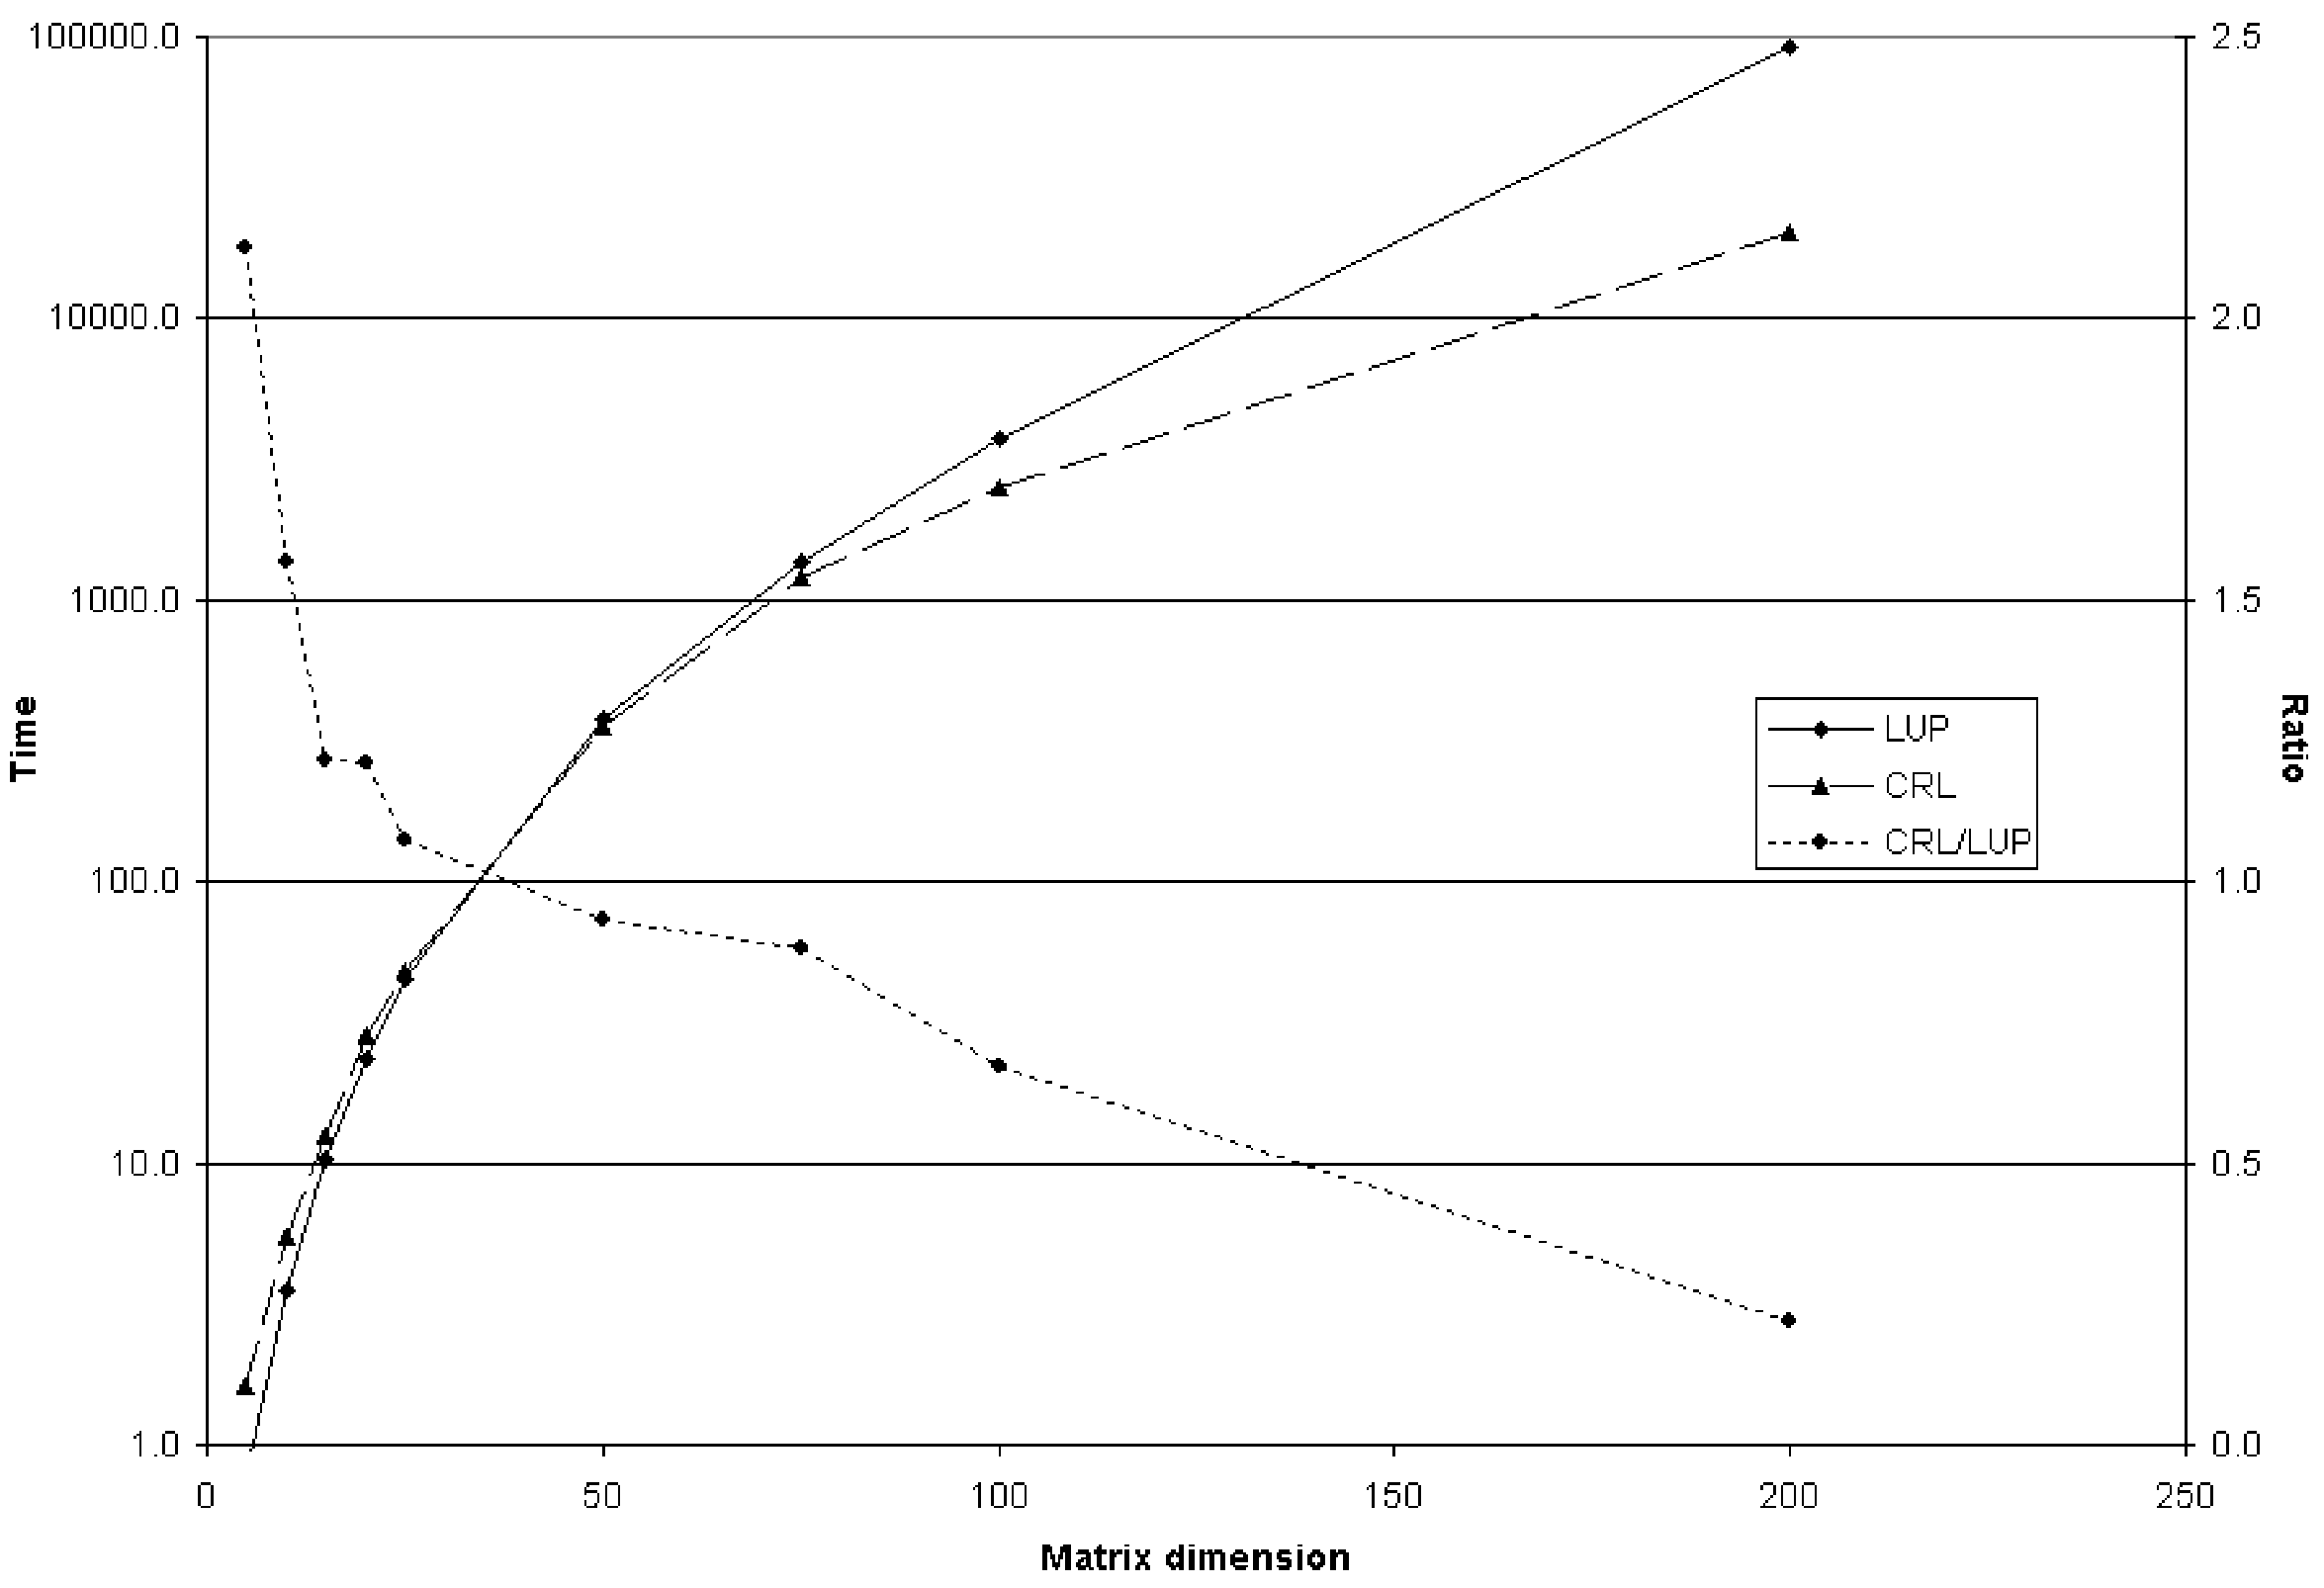
\includegraphics[width=10cm]{Figures/InversionTime}
\caption{Comparison of inversion time for non-symmetrical
matrices}\label{fig:inversionTime}
\end{figure}
Figure \ref{fig:inversionTime} shows the time needed to inverse a
non-symmetrical matrix using CRL algorithm (solid line) and LUP
decomposition (broken line), as well as the ratio between the two
times (dotted line). The CRL algorithm has a large overhead but a
smaller factor for the dependency on dimension. Thus, computing
the inverse of a matrix using LUP decomposition is faster than the
CLR algorithm for small matrices and slower for large matrices. As
a consequence, our implementation of matrix inversion uses a
different algorithm depending on the dimension of the matrix: if
the dimension of the matrix is below a critical dimension, LUP
decomposition is used; otherwise the CRL algorithm is used. In
addition, LUP decomposition is always used if it has already been
computed for another purpose.

On figure \ref{fig:inversionTime} we can determine that the
critical dimension, below which the LUP decomposition works faster
than the CRL algorithm, is about $36$. These data were collected on
a Pentium II running Windows NT 4.0. As this value is depending on
the performance of the operating system, the reader is advised to
determine the critical dimension again when installing the classes
on another system.

In practice, the CLR algorithm described in equations
\ref{eq:crlsplit} to \ref{eq:crlshur} can only be applied to
symmetric matrices. In \cite{CorLeiRiv} Cormen \textit{et al.}
propose to generalize it to matrices of any size by observing the
following identity:
\begin{equation}
\label{eq:pseudoinverse}
  \textbf{A}\cdot\left[\left(\transpose{A}\cdot\textbf{A}\right)^{-1}\cdot\transpose{A}\right]=\textbf{I}
\end{equation}
which can be verified for any matrix $\textbf{A}$. Thus, the
expression in bracket can be considered as the inverse of the
matrix $\textbf{A}$. In mathematics, it is called the pseudo-inverse
or the Moore-Penrose inverse. Since the product
$\transpose{A}\cdot\textbf{A}$ is always a symmetric matrix, its
inverse can be computed with the CRL algorithm. In practice,
however. this technique is plagued with rounding errors and should
be used with caution (\cf section \ref{sec:matrixrounding}).

\subsection{Matrix inversion implementation}
Listing \ref{lst:inversion} shows the complete implementation in
Pharo. It contains additional methods for the classes \code{PMMatrix} and \code{PMSymmetricMatrix}.

For symmetric matrices the method \code{inverse} first tests
whether the dimension of the matrix is below a given threshold ---
defined by the class method \code{lupCRLCriticalDimension} --- or
whether the LUP decomposition of the matrix was already performed.
In that case, the inverse is computed from the LUP decomposition
using the method described at the beginning of section
\ref{sec:matrixinversion}. Otherwise the CRL algorithm is used.
The implementation of the CRL algorithm is straightforward thanks
to the matrix operators defined in section
\ref{sec:slinearalgebra}.

For non-symmetric matrices the method \code{inverse} first tests
whether the matrix is square or not. If the matrix is square, LUP
decomposition is used. If the matrix is not square the pseudo
inverse is computed using equation \ref{eq:pseudoinverse}.

In both cases there is no error handling. Inverting a singular
matrix produces an arithmetic error which must be handled by the
calling method.

\begin{listing}[label=lst:inversion]{Smalltalk}
{Implementation of matrix inversion}
%$$\halign{ #\hfil&\quad#\hfil\cr {\sl Class}& {\Large\bf DhbSymmetricMatrix}\cr
{\sl Subclass of }&{\tt DhbMatrix}\cr\noalign{\vskip 1ex}
}$$


Class methods
{\parskip 1ex\par\noindent}
{\bf join:} {\tt anArrayOfMatrices}
\begin{verbatim}
    | rows n |
    rows := OrderedCollection new.
    n := 0.
    ( anArrayOfMatrices at: 1) rowsDo:
        [ :each |
          n := n + 1.
          rows add: each, ((anArrayOfMatrices at: 3) columnAt: n) ].
    n := 0.
    ( anArrayOfMatrices at: 2) rowsDo:
        [ :each |
          n := n + 1.
          rows add: ((anArrayOfMatrices at: 3) rowAt: n), each ].
    ^ self rows: rows 
\end{verbatim}
{\bf lupCRLCriticalDimension}
\begin{verbatim}
    ^ 36
\end{verbatim}



Instance methods
{\parskip 1ex\par\noindent}
{\bf crlInverse}
\begin{verbatim}
    | matrices b1 cb1ct cb1 |
    matrices := self split.
    b1 := (matrices at: 1) inverse.
    cb1 := (matrices at: 3) * b1.
    cb1ct := (cb1 productWithTransposeMatrix: (matrices at: 3)) 
                asSymmetricMatrix.
    matrices at: 3 put: (matrices at: 2) * cb1.
    matrices at: 2 put: ((matrices at: 2) accumulateNegated: cb1ct) 
                                                              inverse.
    matrices at: 1 put: ( b1 accumulate: (cb1 
                       transposeProductWithMatrix: (matrices at: 3))).
    (matrices at: 3) negate.
    ^ self class join: matrices
\end{verbatim}
{\bf inverse}
\begin{verbatim}
    ^ (rows size < self class lupCRLCriticalDimension or: 
                                           [ lupDecomposition notNil ]) 
            ifTrue: [ self lupInverse ]
            ifFalse: [ self crlInverse ]
\end{verbatim}
{\bf split}
\begin{verbatim}
    | n b d c |
    n := self largestPowerOf2SmallerThan: rows size.
    ^Array with: (self class rows: ((1 to: n) asVector collect: [ 
                               :k | (rows at: k) copyFrom: 1 to: n]))
              with:(self class rows: (((n+1) to: rows size) 
      asVector collect: [ :k | (rows at: k) copyFrom: (n+1) to: rows 
      size]))
              with: (self class superclass rows: (((n+1) to: rows 
     size) asVector collect: [ :k | (rows at: k) copyFrom: 1 to: n]))
\end{verbatim}


%$$\halign{ #\hfil&\quad#\hfil\cr {\sl Class}& {\Large\bf DhbMatrix}\cr
{\sl Subclass of }&{\tt Object}\cr\noalign{\vskip 1ex}

{\sl Instance variable names:}&\parbox[t]{4 in}{\tt  rows lupDecomposition }\cr\noalign{\vskip 1ex}}$$


Class methods
{\parskip 1ex\par\noindent}
{\bf lupCRLCriticalDimension}
\begin{verbatim}
    ^ 40
\end{verbatim}

Instance methods
{\parskip 1ex\par\noindent}
{\bf inverse}
\begin{verbatim}
    ^self isSquare 
        ifTrue: [ self lupInverse ]
        ifFalse: [ self squared inverse * self transpose ]
\end{verbatim}
{\bf largestPowerOf2SmallerThan:} {\tt anInteger}
\begin{verbatim}
    | m m2|
    m := 2.
    [ m2 := m * 2.
      m2 < anInteger ] whileTrue:[ m := m2 ].
    ^ m
\end{verbatim}
{\bf lupInverse}
\begin{verbatim}
    ^ self class rows: self lupDecomposition inverseMatrixComponents
\end{verbatim}


\end{listing}

\subsection{Matrix inversion --- Rounding problems}
\label{sec:matrixrounding} Operations with large matrices are well
known to exhibit serious rounding problems. The reason is that the
computation of the vector product of each row and column is a sum:
the higher the dimension and the longer the sum. For large matrix
dimensions the magnitude of the sum can mask small contributions
from single products. Successive multiplications thus amplify
initial small deviations. This is especially the case when
computing the inverse of a general matrix using the CRL algorithm
combined with the pseudo-inverse (\ref{eq:pseudoinverse}).

Now is the time to unveil the mystery example of section
\ref{sec:roundingintro} about rounding errors propagation. The
problem solved in this example is matrix inversion. The parameter
describing the complexity of the problem is the dimension of the
matrix. This is the quantity plotted along the $x$-axis of figure
\ref{fig:precision}. Let $\textbf{A}$ the matrix to be inverted. The
matrix $\textbf{M}$ defined by
\begin{equation}
  \textbf{M}=\inverse{A}\cdot\textbf{A}-\textbf{I},
\end{equation}
should have all its components equal to zero. The precision of the
result is defined as the largest absolute value over all
components of the matrix $\textbf{M}$. That quantity is plotted along
the $y$-axis of figure \ref{fig:precision}.

Method A computes the inverse of the matrix using LUP
decomposition, method B using the CRL algorithm. The {\textsl general}
data correspond to a matrix whose components were generated by a
random number generator (\cf section \ref{sec:random}). They were
all comprised between 0 and 1. For the {\textsl special} data the
matrix $\textbf{A}$ is a covariance matrix (\cf section
\ref{sec:covmatrix}) obtained by generating 1000 vectors with
random components comprised between 0 and 1. For method B general
data, the inverse of a non-symmetrical matrix is computed using
the CRL algorithm combined with equation \ref{eq:pseudoinverse}.
In this general form, the CRL algorithm is faster the LUP for
matrices of dimensions larger than about 165. The precision,
however, is totally unreliable as can been seen on Figure
\ref{fig:precision}.

\section{Matrix eigenvalues and eigenvectors of a non-symmetric matrix}
\label{sec:eigen} A non-zero vector $\textbf{u}$ is called an {\textsl eigenvector} of the matrix $\textbf{M}$ if there exists a complex number $\lambda$ such that:
\begin{equation}
\label{eq:eigendef}
 \textbf{M}\cdot\textbf{u}=\lambda\textbf{u}.
\end{equation}
the number $\lambda$ is called an \textsl{eigenvalue} of the matrix
$\textbf{M}$. Equation \ref{eq:eigendef} implies that the matrix
$\textbf{M}$ must be a square matrix. In general a non-singular
matrix of dimension $n$ has $n$ eigenvalues and eigenvectors. Some
eigenvalues, however, may be double\footnote{Eigenvalues are the
roots of a polynomial of degree $n$. A double eigenvalue has two
different eigenvectors.}. Discussing the existence of eigenvalues
in the general case goes beyond the scope of this book. Equation
\ref{eq:eigendef} shows that an eigenvector is defined up to a
constant\footnote{If the vector $\textbf{u}$ is an eigenvector of the
matrix $\textbf{M}$ with eigenvalue $\lambda$, so are all vectors
$\alpha\textbf{u}$ for any $\alpha\ne 0$.}. One can prove that two
eigenvectors of the same matrix, but corresponding to two
different eigenvalues, are orthogonal to each other \cite{Bass}.
Thus, the eigenvectors of a matrix form a complete set of
reference in a $n$ dimensional space.

Computing the eigenvalues and eigenvectors of an arbitrary matrix
is a difficult task. Solving this problem in the general case is
quite demanding numerically. In the rest of this section we give
an algorithm which works well when the absolute value of one of
the eigenvalues is much larger than that of the others. The next
section discusses Jacobi's algorithm finding all eigenvalues of a
symmetrical matrix.

For an arbitrary square matrix the eigenvalue with the largest
absolute value can be found with an iterative process. Let ${\textbf
u}$ be an arbitrary vector and let $\lambda_{\max}$ be the
eigenvalue with the largest absolute value. Let us define the
following series of vectors:
\begin{equation}
\left\{
  \begin{array}{lcl}
    \textbf{u}_0 &=& \textbf{u}, \\*[1ex]
    \textbf{u}_k &=& {\displaystyle 1\over\displaystyle\lambda_{\max}}\textbf{M}\cdot{\textbf
    u}_{k-1}\mbox{\quad for $k>0$}.
  \end{array}
\right.
\end{equation}
It is easy to prove\footnote{Hint: one must write the vector ${\textbf
u}$ as a linear combination of the eigenvectors of the matrix
$\textbf{M}$. Such linear combination exists because the eigenvectors
of a matrix form a complete system of reference.} that:
\begin{equation}
  \lim_{k\to\infty}\textbf{u}_k=\textbf{u}_{\max},
\end{equation}
where $\textbf{u}_{\max}$ is the eigenvector corresponding to
$\lambda_{\max}$. Using this property, the following algorithm can
be applied.
\begin{enumerate}
  \item Set $\textbf{u}=\left(1,1,\ldots,1\right)$.
  \item Set $\textbf{u}^{\prime}=\textbf{M}\textbf{u}$.
  \item Set $\lambda=u^{\prime}_1$, that is the first component of the
  vector $\textbf{u}^{\prime}$.
  \item Set $\textbf{u}= {1\over\lambda}\textbf{u}^{\prime}$.
  \item Check for convergence of $\lambda$. Go to step 2 if
  convergence is not yet attained.
\end{enumerate}
The algorithm will converge toward $\lambda_{\max}$ if the initial
vector $\textbf{u}$ is not an eigenvector corresponding to a null
eigenvalue of the matrix $\textbf{M}$. If that is the case, one can
chose another initial vector.

Once the eigenvalue with the largest absolute value has been
found, the remaining eigenvalues can be found by replacing the
matrix $\textbf{M}$ with the matrix:
\begin{equation}
\label{eq:eigennext}
  \textbf{M}^{\prime}=\textbf{M}\cdot\left(\textbf{I}-\textbf{u}_{\max}\otimes{\textbf
  v}_{\max}\right),
\end{equation}
where $\textbf{I}$ is the identity matrix of same dimension as the
matrix $\textbf{M}$ and $\textbf{v}_{\max}$ is the eigenvector of the
matrix $\transpose{M}$ corresponding to
$\lambda_{\max}$\footnote{The transpose of a matrix has the same
eigenvalues, but not necessarily the same eigenvectors.}. Using
the fact that eigenvectors are orthogonal to each other, one can
prove that the matrix $\textbf{M}^{\prime}$ of equation
\ref{eq:eigennext} has the same eigenvalues as the matrix except
for $\lambda_{\max}$ which is replaced by 0. A complete proof of
the above can be found in \cite{Bass}.

All eigenvalues and eigenvectors of the matrix $\textbf{M}$ can be
found by repeating the process above $n$ times. However, this
works well only if the absolute values of the eigenvalues differ
from each consecutive ones by at least an order of magnitude.
Otherwise, the convergence of the algorithm is not very good. In
practice, this algorithm can only be used to find the first couple
of eigenvalues.

\subsection{Finding the largest eigenvalue --- General implementation}
%\marginpar{Figure \ref{fig:linearalgebraclasses} with the box \textbf{LargestEigenValueFinder} grayed.}
The object in charge of finding the largest eigenvalue is of course an instance
of a subclass of the iterative process class described in
\ref{sec:iteration}. As the reader can see very few methods are
required because most of the work is already implemented in the
framework for iterative processes. The implementation is identical
in both languages and will be discussed here. The largest
eigenvalue finder has the following instance variables:
\begin{itemize}
  \item \code{matrix} the matrix whose largest eigenvalue is sought,
  \item \code{eigenValue} the sought eigenvalue,
  \item \code{eigenVector} the sought eigenvector and
  \item \code{transposedEigenVector} the eigenvector of the
  transposed matrix.
\end{itemize}
The creation method takes the matrix as argument. Two accessor
methods are supplied to retrieve the results, the eigenvalue and
the eigenvector.

The method \code{initializeIterations} creates a vector to the
matrix dimension and sets all its components equal to 1. As the
algorithm progresses this vector will contain the eigenvector of
the matrix. Similarly, a vector, which will contain the
eigenvector of the transposed matrix, is created in the same way.
In principle one should add a part to verify that this vector does
not correspond to a null eigenvalue of the matrix. This small
improvement is left as an exercise to the reader.

The algorithm is implemented within the single method \code{evaluateIteration} as described in section \ref{sec:iteration}.
The relative precision of the sought eigenvalue is the precision
used to break out of the iterative process.

Since the algorithm determines both the eigenvalue and the
eigenvector the object in charge of the algorithm keeps both of
them and must give access to both of them. Two accessor methods
are supplied to retrieve the results, the eigenvalue and the
eigenvector.

The largest eigenvalue finder is responsible to create the object
responsible for finding the next eigenvalue when needed. Thus, the
eigenvector of the transposed matrix is also computed along with
the regular eigenvector. The method \code{nextLargestEigenValueFinder} returns a new instance of the class,
which can be used to compute the next largest eigenvalue, by
computing a new matrix as described in equation
\ref{eq:eigennext}.

\subsection{Finding the largest eigenvalue implementation}
Listing \ref{lst:eigenlarge} shows the Pharo implementation of the class \code{PMLargestEigenValueFinder}, subclass of the class \code{PMIterativeProcess}.

The following code example shows how to use the class to find the
first two largest eigenvalues of a matrix.
\begin{displaycode}{Smalltalk}
 | m finder eigenvalue eigenvector nextFinder nextEigenvalue nextEigenvector |
 m := PMMatrix rows: #((84 -79 58 55)
                        (-79 84 -55 -58)
                        (58 -55 84 79)
                        (55 -58 79 84)).
 finder := PMLargestEigenValueFinder matrix: m.
 eigenvalue := finder evaluate.
 eigenvector := finder eigenvector.
 nextFinder := finder nextLargestEigenValueFinder.
 nextEigenvalue := nextFinder evaluate.
 nextEigenvector := nextFinder eigenvector.
\end{displaycode}
First the matrix \code{m} is defined from its components. Then, an
instance of the class \code{PMLargestEigenValueFinder} is created
for this matrix. The iterative process is started as described in
section \ref{sec:siteration}. Its result is the eigenvalue. The
eigenvector is retrieved using an accessor method. Then, a new
instance of \code{PMLargestEigenValueFinder} is obtained from the
first one. The next largest eigenvalue and its eigenvector are
retrieved from this new instance exactly as before.

\begin{listing}[label=lst:eigenlarge]{Smalltalk}
{Implementation of the search for the largest eigenvalue}
%$$\halign{ #\hfil&\quad#\hfil\cr {\sl Class}& {\Large\bf DhbLargestEigenValueFinder}\cr
{\sl Subclass of }&{\tt DhbIterativeProcess}\cr\noalign{\vskip 1ex}

{\sl Instance variable names:}&\parbox[t]{4 in}{\tt  matrix eigenvector transposeEigenvector }\cr\noalign{\vskip 1ex}}$$


Class methods
{\parskip 1ex\par\noindent}
{\bf defaultMaximumIterations}
\begin{verbatim}
    ^ 100
\end{verbatim}
{\bf matrix:} {\tt aMatrix}
\begin{verbatim}
    ^ self new initialize: aMatrix; yourself
\end{verbatim}
{\bf matrix:} {\tt aMatrix} {\bf precision:} {\tt aNumber}
\begin{verbatim}
    ^ self new initialize: aMatrix; desiredPrecision: aNumber; 
                                                              yourself
\end{verbatim}



Instance methods
{\parskip 1ex\par\noindent}
{\bf eigenvalue}
\begin{verbatim}
    ^ result
\end{verbatim}
{\bf eigenvector}
\begin{verbatim}
    ^ eigenvector * (1 / eigenvector norm)
\end{verbatim}
{\bf evaluateIteration}
\begin{verbatim}
    | oldEigenvalue |
    oldEigenvalue := result.
    transposeEigenvector := transposeEigenvector * matrix.
    transposeEigenvector := transposeEigenvector 
                * (1 / (transposeEigenvector at: 1)).
    eigenvector := matrix * eigenvector.
    result := eigenvector at: 1.
    eigenvector := eigenvector * (1 / result).
    ^oldEigenvalue isNil 
        ifTrue: [ 2 * desiredPrecision]
        ifFalse: [ (result - oldEigenvalue) abs ]
\end{verbatim}
{\bf initialize:} {\tt aMatrix}
\begin{verbatim}
    matrix := aMatrix.
\end{verbatim}
{\bf initializeIterations}
\begin{verbatim}
    eigenvector := DhbVector new: matrix numberOfRows.
    eigenvector atAllPut: 1.0.
    transposeEigenvector := DhbVector new: eigenvector size.
    transposeEigenvector atAllPut: 1.0
\end{verbatim}
{\bf nextLargestEigenValueFinder}
\begin{verbatim}
    | norm |
    norm := 1 / (eigenvector * transposeEigenvector).
    ^self class 
        new: matrix * ((DhbSymmetricMatrix identity: eigenvector 
                                                                size) 
                        - (eigenvector * norm tensorProduct: 
                                                transposeEigenvector))
        precision: desiredPrecision
\end{verbatim}


\end{listing}

\section{Matrix eigenvalues and eigenvectors of a symmetric matrix}
\label{sec:eigensym}
In the nineteen century Carl Jacobi discovered an efficient
algorithm to find the eigenvalues of a symmetric matrix. Finding
the eigenvalues of a symmetric matrix is easier since all
eigenvalues are real.

In the section \ref{sec:eigen} we have mentioned that the
eigenvectors of a matrix are orthogonal. Let $\textbf{u}^{\left( 1
\right)},\ldots,\textbf{u}^{\left( n \right)}$ the set of
eigenvectors of the matrix $\textbf{M}$ such that ${\textbf
u}^{\left(i\right)}\cdot\textbf{u}^{\left(i\right)}=1$ for all $i$.
Then, the matrix
\begin{equation}
  \textbf{O}=\pmatrix{u^{\left(1\right)}_1& u^{\left(2\right)}_1&\ldots& u^{\left(n\right)}_1\cr
  u^{\left(1\right)}_2& u^{\left(2\right)}_2&\ldots& u^{\left(n\right)}_2\cr
  \vdots&\vdots&\ddots&\vdots\cr
  u^{\left(1\right)}_n& u^{\left(2\right)}_n&\ldots&
  u^{\left(n\right)}_n\cr},
\end{equation}
where $u^{\left(k\right)}_i$ is the $i^{\mathop\textrm{th}}$
component of the $k^{\mathop\textrm{th}}$ eigenvector,is an
orthogonal\footnote{An orthogonal matrix of dimension $n$ is a
rotation in the $n$-dimensional space.} matrix. That is, we have:
\begin{equation}
\label{eq:orthomatrix} \transpose{O}\cdot\textbf{O}=\textbf{I}.
\end{equation}
Equation \ref{eq:orthomatrix} is just another way of stating that
the vectors $\textbf{u}^{\left( 1 \right)},\ldots,\textbf{u}^{\left( n
\right)}$ are orthogonal to each other and are all normalized to
1. Combining this property with the definition of an eigenvector
(equation \ref{eq:eigendef}) yields:
\begin{equation}
\transpose{O}\cdot\textbf{M}\cdot\textbf{O}=\pmatrix{\lambda_1&
0&\ldots&0\cr
  0& \lambda_2&\ldots& 0\cr
  \vdots&\vdots&\ddots&\vdots\cr
  0& 0&\ldots&\lambda_n\cr},
\end{equation}
where $\lambda_1,\ldots,\lambda_n$ are the eigenvalues of the
matrix $\textbf{M}$.

The gist of Jacobi's algorithm is to apply a series of orthogonal
transformations such that the resulting matrix is a diagonal
matrix. It uses the fact that, for any orthogonal matrix ${\textbf
R}$, the matrix $\transpose{R}\textbf{M}\cdot\textbf{R}$ has the same
eigenvalues as the matrix $\textbf{M}$. This follows from the
definition of an eigenvector (equation \ref{eq:eigendef}) and the
property of an orthogonal matrix (equation \ref{eq:orthomatrix}).

An orthogonal matrix corresponds to a rotation of the system of
reference axes. Each step of Jacobi's algorithm is to find an
rotation, which annihilates one of the off-diagonal elements of
the matrix resulting from that orthogonal transformation. Let
$\textbf{R}_1$ be such matrix and let us define
\begin{equation}
  \textbf{M}_1 = \transpose{R}_1\cdot\textbf{M}\cdot\textbf{R}_1.
\end{equation}
Now, let us define the orthogonal transformation $\textbf{R}_2$,
which annihilates one of the off-diagonal elements of the matrix
$\textbf{M}_1$. The hope is that, after a certain number of steps
$m$, the matrix
\begin{equation}
  \begin{array}{lcl}
    \textbf{M}_m & = &\transpose{R}_m\cdot\textbf{M}_{m-1}\cdot{\textbf
    R}_m\\*[2ex]
      & = &\transpose{R}_m\cdots\transpose{R}_1\cdot\textbf{M}\cdot{\textbf
      R}_1\cdots\textbf{R}_m
  \end{array}
\end{equation}
becomes a diagonal matrix. Then the diagonal elements of the
matrix $\textbf{M}_m$ are the eigenvalues and the matrix
\begin{equation}
    \textbf{O}_m = \textbf{R}_1\cdots\textbf{R}_m
\end{equation}
is the matrix containing the eigenvectors.

Instead of annihilating just any diagonal element, one tries to
annihiliate the element with the largest absolute value. This
ensures the fastest possible convergence of the algorithm. Let
$m_{kl}$ be the off-diagonal element of the matrix $\textbf{M}$ with
the largest absolute value. We define a matrix $\textbf{R}_1$ with
components:
\begin{equation}
  \left\{
  \begin{array}{lcl}
    r^{\left(1\right)}_{kk} &=& \cos\vartheta, \\*[2ex]
    r^{\left(1\right)}_{ll} &=& \cos\vartheta, \\*[2ex]
    r^{\left(1\right)}_{kl} &=& -\sin\vartheta, \\*[2ex]
    r^{\left(1\right)}_{lk} &=& \sin\vartheta, \\*[2ex]
    r^{\left(1\right)}_{ii} &=& 1\mbox{\quad for $i\ne k,l$}, \\*[2ex]
    r^{\left(1\right)}_{ij} &=& 0\mbox{\quad for $i\ne j, i$ and $j \ne k,l$.}
  \end{array}
  \right.
\end{equation}
The reader can verify that the matrix $\textbf{R}_1$ is an orthogonal
matrix. The new matrix $\textbf{M}_1=\transpose{R}_1\cdot\textbf{
M}\cdot\textbf{R}_1$ has the same components as the matrix $\textbf{M}$
except for the rows and columns $k$ and $l$. That is, we have
\begin{equation}
\label{eq:jacobistep}
  \left\{
  \begin{array}{lcl}
    m^{\left(1\right)}_{kk} &=& \cos^2\vartheta m_{kk}+\sin^2\vartheta m_{ll} - 2\sin\vartheta\cos\vartheta m_{kl}, \\*[2ex]
    m^{\left(1\right)}_{ll} &=& \sin^2\vartheta m_{kk}+\cos^2\vartheta m_{ll} + 2\sin\vartheta\cos\vartheta m_{kl}, \\*[2ex]
    m^{\left(1\right)}_{kl} &=& \left(\cos^2\vartheta-\sin^2\vartheta\right)m_{kl}+\sin\vartheta\cos\vartheta
    \left(m_{kk}-m_{ll}\right), \\*[2ex]
    m^{\left(1\right)}_{ik} &=& \cos\vartheta m_{ik}-\sin\vartheta m_{il}\mbox{\quad for $i\ne k,l$}, \\*[2ex]
    m^{\left(1\right)}_{il} &=& \cos\vartheta m_{il}+\sin\vartheta m_{ik}\mbox{\quad for $i\ne k,l$}, \\*[2ex]
    m^{\left(1\right)}_{ij} &=& m_{ij}\mbox{\quad for $i\ne k,l$ and $j\ne k,l$}.  \end{array}
  \right.
\end{equation}
In particular, the angle of rotation can be selected such that
$m^{\left(1\right)}_{kl}=0$. That condition yields the following
equation for the angle of the rotation:
\begin{equation}
\label{eq:jacobirot}
  {\cos^2\vartheta-\sin^2\vartheta
  \over\sin\vartheta\cos\vartheta}={m_{ll} - m_{kk}\over
  m_{kl}}=\alpha,
\end{equation}
where the constant $\alpha$ is defined by equation
\ref{eq:jacobirot}. Introducing the variable $t=\tan\vartheta$,
equation \ref{eq:jacobirot} can be rewritten as:
\begin{equation}
\label{eq:jacobi2nd}
  t^2+2\alpha t - 1 =0.
\end{equation}
Since equation \ref{eq:jacobi2nd} is a second order equation,
there are two solutions. To minimize rounding errors, it is
preferable to select the solution corresponding to the smallest
rotation\cite{Press}. The solution of equation \ref{eq:jacobi2nd}
has already been discussed in section \ref{sec:outsmart} for the
case where $\alpha$ is positive. For any $\alpha$, it can be
written as:
\begin{equation}
\label{eq:jacobisolinverse}
  t={\displaystyle\sign\left(\alpha\right)\over\displaystyle\left|\alpha\right|+\sqrt{\alpha^2+1}}.
\end{equation}
In fact, the value of the angle $\vartheta$ does not need to be
determined. We have:
\begin{equation}
  \left\{
  \begin{array}{lcl}
    \cos\vartheta&=&{\displaystyle 1\over\displaystyle
    \sqrt{t^2+1}},\\*[2ex]
    \sin\vartheta&=&t\cos\vartheta. \end{array}
  \right.
\end{equation}
Let us now introduce the quantities $\sigma$ and $\tau$ defined as
\begin{equation}
  \left\{
  \begin{array}{lcl}
    \sigma&=&\sin\vartheta,\\*[2ex]
    \tau&=&{\displaystyle\sin\vartheta \over\displaystyle 1+\cos\vartheta}.\end{array}
  \right.
\end{equation}
Then equations \ref{eq:jacobistep} can be rewritten as
\begin{equation}
\label{eq:jacobistepfinal}
  \left\{
  \begin{array}{lcl}
    m^{\left(1\right)}_{kk} &=& m_{kk} - t m_{kl}, \\*[2ex]
    m^{\left(1\right)}_{ll} &=& m_{ll} + t m_{kl}, \\*[2ex]
    m^{\left(1\right)}_{kl} &=& 0, \\*[2ex]
    m^{\left(1\right)}_{ik} &=& m_{ik}-\sigma\left( m_{il}+\tau m_{ik}\right)\mbox{\quad for $i\ne k,l$}, \\*[2ex]
    m^{\left(1\right)}_{il} &=& m_{il}+\sigma\left( m_{ik}-\tau m_{il}\right)\mbox{\quad for $i\ne k,l$}, \\*[2ex]
    m^{\left(1\right)}_{ij} &=& m_{ij}\mbox{\quad for $i\ne k,l$ and $j\ne k,l$}.  \end{array}
  \right.
\end{equation}

Finally, we must prove that the transformation above did not
increase the absolute values of the remaining off-diagonal
elements of the matrix $\textbf{M}_1$. Using equations
\ref{eq:jacobistep} the sum of the off-diagonal elements of the
matrix $\textbf{M}_1$ is:
\begin{equation}
\label{eq:jacobiconv}
  \sum_{i\ne j}\left(m^{\left(1\right)}_{ij}\right)^2=\sum_{i\ne j}m_{ij}^2-2 m^2_{kl}.
\end{equation}
Thus, this sum is always less that the sum of the squared
off-diagonal elements of the matrix $\textbf{M}$. In other words the
algorithm will always converge.

\rubrique{Jacobi's algorithm} Now we have all the elements to
implement Jacobi's algorithm. The steps are described hereafter:
\begin{enumerate}
  \item Set the matrix $\textbf{M}$ to the matrix whose eigenvalues
  are sought.
  \item Set the matrix $\textbf{O}$ to an identity matrix of the same
  dimension as the matrix $\textbf{M}$.
  \item Find the largest off-diagonal element, $m_{kl}$, of the matrix $\textbf{
  M}$.
  \item Build the orthogonal transformation $\textbf{R}_1$
  annihilating the element $m_{kl}$.
  \item Build the matrix $\textbf{M}_1=\transpose{R}_1\cdot\textbf{M}\cdot\textbf{
  R}_1$.
  \item If $\left|m_{kl}\right|$ is less than the desired
  precision go to step 8.
  \item Let $\textbf{M}=\textbf{M}_1$ and $\textbf{O}=\textbf{O}\cdot\textbf{R}_1$; go to step 3.
  \item The eigenvalues are the diagonal elements of the matrix $\textbf{
  M}$ and the eigenvectors are the rows of the matrix $\textbf{O}$.
\end{enumerate}
Strictly speaking, Jacobi's algorithm should be stopped if the
largest off-diagonal element of matrix $\textbf{M}_1$ is less than
the desired precision. However, equation \ref{eq:jacobiconv}
guaranties that the largest off-diagonal element of the matrix
after each step of Jacobi's algorithm is always smaller that the
largest off-diagonal element of the matrix before the step. Thus.
the stopping criteria proposed above can safely be used. This
slight overkill prevents us from scanning the off-diagonal
elements twice per step.

As the algorithm converges, $\alpha$ becomes very large. As
discussed in section \ref{sec:outsmart}, the solution of equation
\ref{eq:jacobi2nd} can be approximated with
\begin{equation}
  t\approx{\displaystyle 1\over\displaystyle 2\alpha}.
\end{equation}
This expression is used when the computation of $\alpha^2$ causes
an overflow while evaluating equation \ref{eq:jacobisolinverse}.

\subsection{Jacobi's algorithm --- General implementation}
%\marginpar{Figure \ref{fig:linearalgebraclasses} with the box \textbf{ JacobiTransformation} grayed.}
Jacobi's algorithm is an iterative algorithm.
The object implementing Jacobi's algorithm is a instance of the class \code{JacobiTransform}; it is a subclass of the iterative process discussed in section \ref{sec:iteration}.
%The instance variables of this class are different in the two language implementations.

When an instance of the class \code{JacobiTransform} is created,
the matrix whose eigenvalues are sought is copied into the matrix
$\textbf{M}$. This permits to use the same storage over the duration
of the algorithm since equations \ref{eq:jacobistepfinal} can be
evaluated in place. Actually, only the upper half of the
components needs to be stored since the matrix is a symmetric
matrix.

The method \code{evaluateIteration} finds the largest off-diagonal
element and performs the Jacobi step (equations
\ref{eq:jacobistepfinal}) for that element. During the search for
the largest off-diagonal element, the precision of the iterative
process is set to the absolute value of the largest off-diagonal
element. This is one example where it does not make sense to
compute a relative precision. Actually, the precision returned by
the method \code{evaluateIteration} is that of the previous
iteration, but it does not really matter to make one iteration too
much.

The method \code{finalizeIterations} performs a bubble sort to
place the eigenvalues in decreasing order of absolute value.
Bubble sorting is used instead of using a \code{SortedCollection}
because one must also exchange the corresponding eigenvectors.

The result of the iterative process is an array containing the
sorted eigenvalues plus the transformation matrix $\textbf{O}$
containing the eigenvectors. Extracting these results is language
dependent.

\subsection{Jacobi's algorithm implementation}
Listing \ref{lst:jacobi} shows the implementation of Jacobi's algorithm.

The following code example shows how to use the class to find the
eigenvalues and eigenvectors of a symmetric matrix.
\begin{displaycode}{Smalltalk}
 | m jacobi eigenvalues eigenvectors |
 m := PMSymmetricMatrix rows: #((84 -79 58 55)
                                 (-79 84 -55 -58)
                                 (58 -55 84 79)
                                 (55 -58 79 84)).
 jacobi := PMJacobiTransformation matrix: m.
 eigenvalues := jacobi evaluate.
 eigenvectors := jacobi transform columnsCollect: [ :each | each].
\end{displaycode}
First the matrix \code{m} is defined from its components. Then, an
instance of the class \code{PMJacobiTransformation} is created for
this matrix. The iterative process is started as described in
section \ref{sec:siteration}. Its result is an array containing
the eigenvalues sorted in decreasing order. The corresponding
eigenvectors are retrieved from the columns of the matrix $\textbf{O}$ obtained from the method \code{transform}.

The class \code{PMJacobiTransformation} has two instance variables
\begin{itemize}
  \item \code{lowerRows} an array of array containing the lower part
  of the matrix and
  \item \code{transform} the components of the matrix $\textbf{O}$.
\end{itemize}
Since the matrix $\textbf{M}$ is symmetric there is no need to keep
all of its components. This not only reduces storage but also
speeds up somewhat the algorithm because one only need to
transform the lower part of the matrix.

The instance variable \code{result} contains the sorted eigenvalues
at the end of the iterative process. The method \code{transform}
returns the symmetric matrix ${\textbf{O}}$ whose columns contain the
eigenvectors in the same order. The code example shown at the
beginning of this section shows how to obtain the eigenvectors
from the matrix.

\begin{listing}[label=lst:jacobi]{Smalltalk}
{Implementation of Jacobi's algorithm }
%$$\halign{ #\hfil&\quad#\hfil\cr {\sl Class}& {\Large\bf DhbJacobiTransformation}\cr
{\sl Subclass of }&{\tt DhbIterativeProcess}\cr\noalign{\vskip 1ex}

{\sl Instance variable names:}&\parbox[t]{4 in}{\tt  lowerRows transform }\cr\noalign{\vskip 1ex}}$$


Class methods
{\parskip 1ex\par\noindent}
{\bf matrix:} {\tt aSymmetricMatrix}
\begin{verbatim}
    ^ super new initialize: aSymmetricMatrix
\end{verbatim}
{\bf new}
\begin{verbatim}
    ^ self error: 'Illegal creation message for this class'
\end{verbatim}

Instance methods
{\parskip 1ex\par\noindent}
{\bf evaluateIteration}
\begin{verbatim}
    | indices |
    indices := self largestOffDiagonalIndices.
    self transformAt: (indices at: 1) and: (indices at: 2).
    ^ precision

\end{verbatim}
{\bf exchangeAt:} {\tt anInteger}
\begin{verbatim}
    | temp n |
    n := anInteger + 1.
    temp := result at: n.
    result at: n put: ( result at: anInteger).
    result at: anInteger put: temp.
    transform do:
        [ :each |
          temp := each at: n.
          each at: n put: ( each at: anInteger).
          each at: anInteger put: temp ].
\end{verbatim}
{\bf finalizeIterations}
\begin{verbatim}
    | n |
    n := 0.
    result := lowerRows collect: 
                    [ :each | 
                    n := n + 1.
                    each at: n ].
    self sortEigenValues
\end{verbatim}
{\bf initialize:} {\tt aSymmetricMatrix}
\begin{verbatim}
    | n m |
    n := aSymmetricMatrix numberOfRows.
    lowerRows := Array new: n.
    transform := Array new: n.
    1 to: n do:
        [ :k |
          lowerRows at: k put: ( ( aSymmetricMatrix rowAt: k) 
                                                   copyFrom: 1 to: k).
          transform at: k put: ( ( Array new: n) atAllPut: 0; at: k 
                                                    put: 1; yourself) ].
    ^ self
\end{verbatim}
{\bf largestOffDiagonalIndices}
\begin{verbatim}
    | n m abs |
    n := 2.
    m := 1.
    precision := ( ( lowerRows at: n) at: m) abs.
    1 to: lowerRows size do:
        [ :i |
          1 to: ( i - 1) do:
            [ :j |
              abs := ( ( lowerRows at: i) at: j) abs.
              abs > precision
                ifTrue: [ n := i.
                          m := j.
                          precision := abs ] ] ].
    ^ Array with: m with: n
\end{verbatim}
{\bf printOn:} {\tt aStream}
\begin{verbatim}
    | first |
    first := true.
    lowerRows do: 
        [ :each |
          first ifTrue: [ first := false ]
                 ifFalse: [ aStream cr ].
          each printOn: aStream ].
\end{verbatim}
{\bf sortEigenValues}
\begin{verbatim}
    | n bound m |
    n := lowerRows size.
    bound := n.
    [ bound = 0 ]
        whileFalse: [ m := 0.
                      1 to: bound - 1 do:
                        [ :j |
                          (result at: j) abs > (result at: j + 1) abs
                            ifFalse: [ self exchangeAt: j.
                                      m := j ] ].
                        bound := m ].
\end{verbatim}
{\bf transform}
\begin{verbatim}
    ^ DhbMatrix rows: transform
\end{verbatim}
{\bf transformAt:} {\tt anInteger1} {\bf and:} {\tt anInteger2}
\begin{verbatim}
    | d t s c tau apq app aqq arp arq |
    apq := ( lowerRows at: anInteger2) at: anInteger1.
    apq = 0
        ifTrue: [ ^ nil ].
    app := (lowerRows at: anInteger1) at: anInteger1.
    aqq := (lowerRows at: anInteger2) at: anInteger2.
    d := aqq - app.
    arp := d * 0.5 / apq.
    t := arp > 0 
        ifTrue: [ 1 / ( ( arp squared + 1) sqrt + arp)]
        ifFalse:[ 1 / ( arp - ( arp squared + 1) sqrt)].
    c := 1 / ( t squared + 1) sqrt.
    s := t * c.
    tau := s / ( 1 + c).
    1 to: (anInteger1 - 1)
        do: [ :r |
              arp := (lowerRows at: anInteger1) at: r.
              arq := (lowerRows at: anInteger2) at: r.
              (lowerRows at: anInteger1) at: r put: ( arp - ( s * 
                                                  (tau * arp + arq))).
              (lowerRows at: anInteger2) at: r put: ( arq + ( s * 
                                                (arp - (tau * arq)))).
            ].
    ( anInteger1 + 1) to: ( anInteger2 - 1)
        do: [ :r |
              arp := (lowerRows at: r) at: anInteger1.
              arq := (lowerRows at: anInteger2) at: r.
              (lowerRows at: r) at: anInteger1 put: ( arp - ( s * 
                                                  (tau * arp + arq))).
              (lowerRows at: anInteger2) at: r put: ( arq + ( s * 
                                                (arp - (tau * arq)))).
            ].
    ( anInteger2 + 1) to: lowerRows size
        do: [ :r |
              arp := ( lowerRows at: r) at: anInteger1.
              arq := ( lowerRows at: r) at: anInteger2.
              (lowerRows at: r) at: anInteger1 put: ( arp - ( s * 
                                                  (tau * arp + arq))).
              (lowerRows at: r) at: anInteger2 put: ( arq + ( s * 
                                                (arp - (tau * arq)))).
            ].
    1 to: lowerRows size
        do: [ :r |
              arp := ( transform at: r) at: anInteger1.
              arq := ( transform at: r) at: anInteger2.
              (transform at: r) at: anInteger1 put: ( arp - ( s * 
                                                  (tau * arp + arq))).
              (transform at: r) at: anInteger2 put: ( arq + ( s * 
                                                (arp - (tau * arq)))).
            ].
    (lowerRows at: anInteger1) at: anInteger1 put: ( app - (t * 
                                                                apq)).
    (lowerRows at: anInteger2) at: anInteger2 put: ( aqq + (t * 
                                                                apq)).
    (lowerRows at: anInteger2) at: anInteger1 put: 0.
\end{verbatim}


\end{listing}

%\ifx\wholebook\relax\else\end{document}\fi


%%\ifx\wholebook\relax\else
%\documentclass[twoside]{book}
%\usepackage[active]{srcltx}
%\usepackage[LY1]{fontenc}
%\usepackage{url}
\makeatletter
\def\url@leostyle{%
  \@ifundefined{selectfont}{\def\UrlFont{\sf}}{\def\UrlFont{\sffamily}}}
\makeatother
% Now actually use the newly defined style.
\urlstyle{leo}

\usepackage{graphicx}
\def\etc{{\textit{etc}}}
\def\eg{{\textit{e.g.}}}
\def\ie{{\textit{i.e.}}}
\def\cf{{\textit{c.f.}}\ }
\def\erf{\mathop{\textrm{erf}}}
\def\sign{\mathop{\textrm{sign}}}
\def\prob{\mathop{\textrm{Prob}}}
\def\var{\mathop{\textrm{var}}}
\def\mod{\mathop{\textrm{mod}}}
\def\cor{\mathop{\textrm{cor}}}
\def\cov{\mathop{\textrm{cov}}}
\def\cl{\mathop{\textrm{CL}}}
\def\kg{\mathop{\textrm{Kg}}}
\def\patstyle#1{{\textsc #1}}
\def\th{^{\mathop{\textrm{th}}}}
%\def\st#1{^{\mathop{\rm #1}}}
\def\note#1{\begin{quote}{\textbf{Note:}} #1\end{quote}}
\def\braket#1{\left\langle #1\right\rangle}
\def\order#1{\let\o=#1$\mathcal{O}$\ifx\o 1$\left(n\right)$\else$\left(n^{#1}\right)$\fi}
%\newtheorem{privListing}{Listing}[chapter]
%\newenvironment{listing}{\vskip 3ex\hrule\vskip 1ex\begin{privListing}}{\end{privListing}\hrule\vskip 1ex}
\newtheorem{privExample}{Code example}[chapter]
\newenvironment{codeExample}{\begin{privExample}\begin{quote}\tt}{\end{quote}\end{privExample}}
\def\relboxl#1#2{\hbox to #1\hsize{#2\hfil}}
\def\relboxc#1#2{\hbox to #1\hsize{\hfil #2\hfil}}
\def\relboxr#1#2{\hbox to #1\hsize{\hfil #2}}
\def\transpose#1{\textbf{#1}^{\mathop\textrm{T}}}
\def\inverse#1{\textbf{#1}^{-1}}
%\def\tm{$^{\mathop{\rm TM}}$}
\def\tm{ }
\newenvironment{mainEquation}{\marginpar[\vspace{3 ex} Main
equation$\Rightarrow$]{\vspace{3 ex}$\Leftarrow$Main
equation}\begin{equation}}{\end{equation}}
\def\rubrique#1{\paragraph{#1}\hfil\par\noindent}

%\begin{document}
%\fi

\chapter{Elements of statistics}
\label{ch:statistics} \vspace{1 ex}
\begin{flushright} {\textsl La statistique est la premi\`ere des sciences inexactes.}\footnote{Statistics is the first of the inexact sciences.}\\
Edmond et Jules de Goncourt
\end{flushright}
\vspace{1 ex} Statistical analysis comes into play when dealing
with a large amount of data. Obtaining information from the
statistical analysis of data is the subject of chapter
\ref{ch:estimation}. Some sections of chapter \ref{ch:datamining}
are also using statistics. Concepts needed by statistics are based
on probability theory.

This chapter makes a quick overview of the concepts of probability
theory. It is the third (and last) chapter of this book where most
of the material is not useful {\textit per se}.
Figure \ref{fig:statisticsclasses} shows the classes described in this
chapter.
\begin{figure}
\centering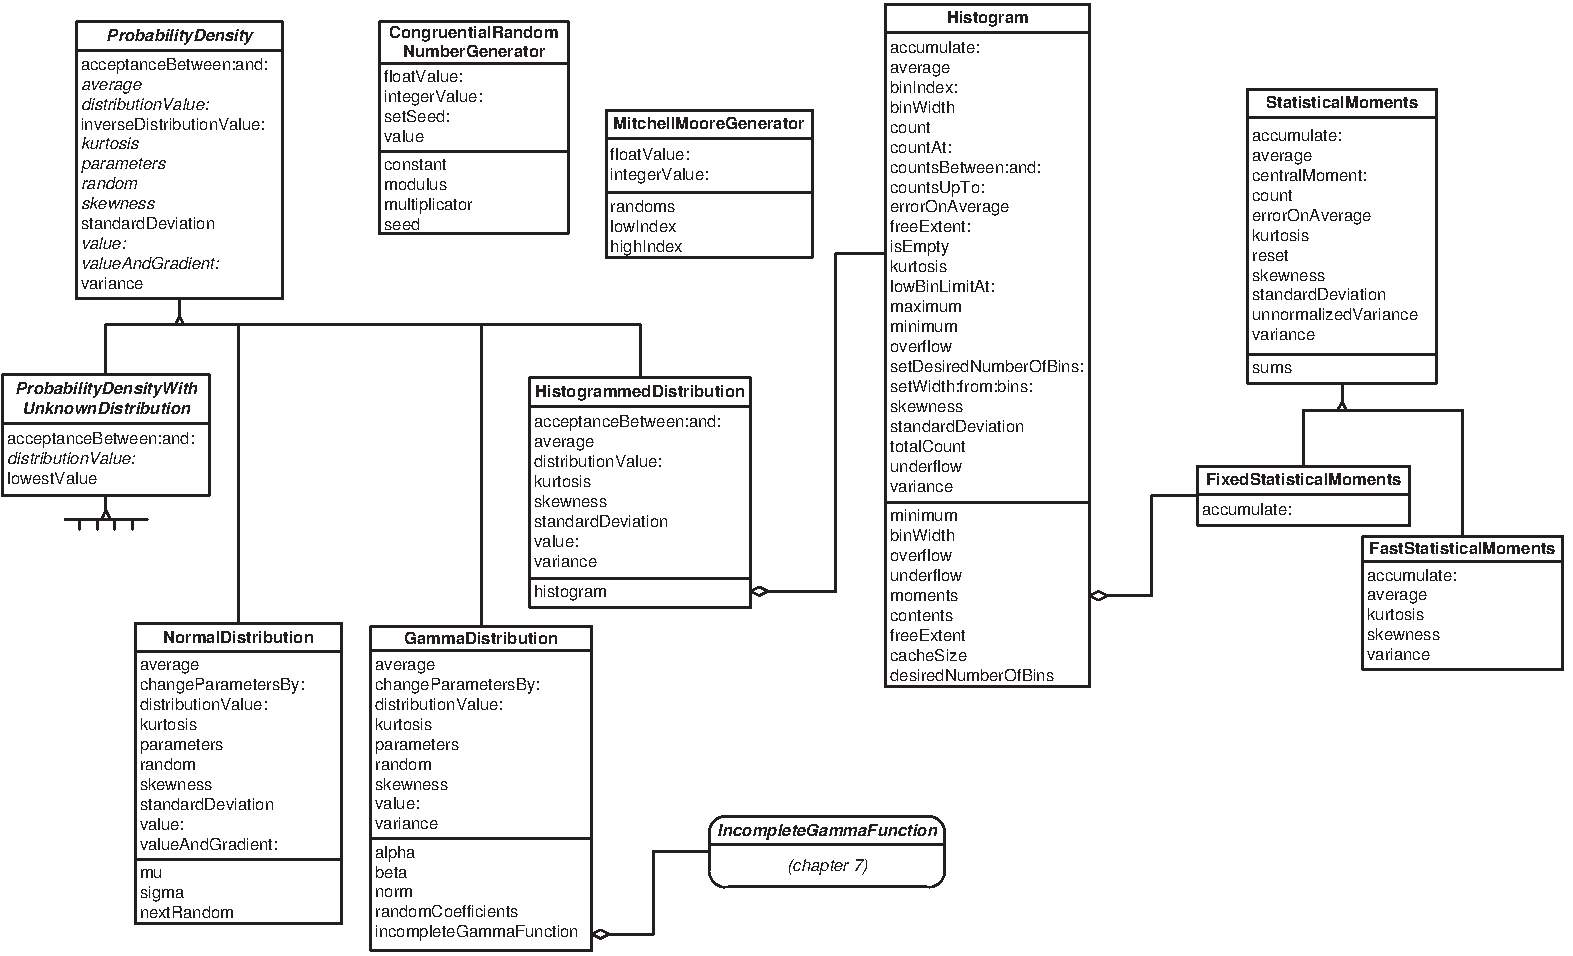
\includegraphics[width=11cm]{Figures/StatisticsClasses}
\caption{Classes related to statistics}
\label{fig:statisticsclasses}
\end{figure}
All these classes, however, are used extensively in the remaining
chapters of this book. The example on how to use the code are kept
to a minimum since real examples of use can be found in the next
chapters.

An in-depth description of probability theory is beyond the scope
of this book. The reader in the need for additional should consult
the numerous textbooks on the subject, \cite{PhiTay} or
\cite{LawKel} for example.

\section{Statistical moments}
\label{sec:moments} When one measures the values of an observable
random variable, each measurement gives a different magnitude.
Assuming measurement errors are negligible, the fluctuation of the
measured values correspond to the distribution of the random
variable. The problem to be solved by the experimenter is to
determine the parameters of the distribution from the observed
values. {\textsl Statistical moments} can contribute to the
characterization of the distribution\footnote{Central moments are
related to the coefficients of the Taylor expansion of the Fourier
transform of the distribution function.}.

Given a set of measurements, $x_1,\ldots,x_n$, of the values
measured for a random variable one defines the moment of $k\th$
order by:
\begin{equation}
  M_k={1\over n}\sum_{i=1}^n x_i^k.
\end{equation}
In particular, the moment of first order is the mean or average of
the set of data:
\begin{equation}
\label{eq:average}
  \bar{x}=M_1={1\over n}\sum_{i=1}^n x_i.
\end{equation}
The central moments of $k^{\mathop{\textrm th}}$ order is defined by:
\begin{equation}
  m_k={1\over n}\sum_{i=1}^n \left(x_i-\bar{x}\right)^k.
\end{equation}
where $k$ is larger than 1. The central moments are easily
expressed in terms of the moments. We have:
\begin{equation}
  m_k=\sum_{j=0}^k \left({k \atop j}\right)\left(-\bar{x}\right)^{k-j}M_j,
\end{equation}
where $\left({k \atop j}\right)$ are the binomial coefficients.

Some statistical parameters are defined on the central moments.
The variance of a set of measurement is the central moment of
second order. The standard deviation, $s$, is the square root of
the variance given by the following formula:
\begin{equation}
s^2={\displaystyle n \over \displaystyle n-1}m_2 ={\displaystyle 1
\over \displaystyle n-1} \sum_{i=1}^n \left(x_i-\bar{x}\right)^2.
\end{equation}
The factor in front the central moment of second order is called
Bessel's correction factor. This factor removes the bias of the
estimation when the standard deviation is evaluated over a finite
sample. The standard deviation measures the spread of the data
around the average.

Many people believe that the standard deviation is the error of
the average. This is not true: the standard deviation describes
how much the data are spread around the average. It thus
represents the error of a single measurement. An estimation of the
standard deviation of the average value is given by the following
formula:
\begin{equation}
\label{eq:averagerror}
  s_{\bar{x}}^2={\displaystyle s^2 \over n}
  \mbox{\quad or \quad}
  s_{\bar{x}}={\displaystyle s \over \sqrt{n}}.
\end{equation}
This expression must be taken as the error on the average when
performing a least square fit on averaged data, for example.

Two quantities are related to the central moments of $3\st{rd}$
and $4\th$ order. Each of these quantities are normalized by the
adequate power of the standard deviation needed to yield a
quantity without dimension.

\noindent The skewness is defined by:
\begin{equation}
  a={\displaystyle n \over\displaystyle
  \left(n-1\right)\left(n-2\right)s^3}m_3
  ={\displaystyle 1 \over\displaystyle
  \left(n-1\right)\left(n-2\right)}
  \sum_{i=1}^n\left({\displaystyle x_i-\bar{x}\over\displaystyle s}\right)^3.
\end{equation}
The skewness is a measure of the asymmetry of a distribution. If
the skewness is positive, the observed distribution is asymmetric
toward large values and vice-versa.

\noindent The kurtosis is defined by
\begin{equation}
\label{eq:kurtosis}
  \begin{array}{rl}
    k=& {\displaystyle n\left(n+1\right) \over\displaystyle
  \left(n-1\right)\left(n-2\right)\left(n-3\right)s^4}m_4 -{\displaystyle 3\left(n-1\right)^2 \over\displaystyle
  \left(n-2\right)\left(n-3\right)}\\*[2ex]
    =& {\displaystyle \left(n+1\right) \over\displaystyle
  \left(n-1\right)\left(n-2\right)\left(n-3\right)}
  \displaystyle\sum_{i=1}^n\left({\displaystyle x_i-\bar{x}\over\displaystyle s}\right)^4 -{\displaystyle 3\left(n-1\right)^2 \over\displaystyle
  \left(n-2\right)\left(n-3\right)}
  \end{array}
\end{equation}
The kurtosis is a measure of the peakedness or flatness of a
distribution in the region of the average. The subtracted term in
equation \ref{eq:kurtosis} is a convention defining the kurtosis
of the normal distribution as 0\footnote{One talks about a {\textsl
platykurtic} distribution when the kurtosis is negative, that is
the peak of the distribution is flatter than that of the normal
distribution. Student (\cf section \ref{sec:ttest}) and Cauchy
(\cf section \ref{sec:cauchydist}) distributions are platykurtic.
The opposite is called {\textsl leptokurtic}. The Laplace (\cf section
\ref{sec:laplacedist}) distribution is leptokurtic. }.

As we have seen, the average, standard deviation, skewness and
kurtosis are parameters, which helps characterizing a distribution
of observed values. To keep track of these parameters, it is handy
to define an object whose responsibility is to accumulate the
moments up to order 4. One can then easily compute the parameters
of the distribution. It can be used in all cases where
distribution parameters are needed.

\subsection{Statistical moments --- Smalltalk implementation}
\marginpar{Figure \ref{fig:statisticsclasses} with the box {\textbf
FastStatisticalMoments} grayed.} To describe this implementation
we must anticipated on the next section: the class {\textbf
FastStatisticalMoments} implementing statistical moments as
described in Section \ref{sec:moments} is a subclass of the class
defined in section \ref{sec:robustmoment}.

Space allocation is handled by the superclass. The class {\texttt
FastStatisticalMoments} uses this allocation to store the moments
(instead of the central moments). The method {\texttt accumulate:}
perform the accumulation of the moments. The methods {\texttt
average}, {\texttt variance}, {\texttt skewness} and {\texttt kurtosis}
compute the respective quantities using explicit expansion of the
central moments as a function of the moments.

The computation of the standard deviation and of the error on the
average are handled by the superclass (\cf listing
\ref{ls:genmoments}).

\label{sec:smoments}Listing \ref{ls:fastmoments} shows the
Smalltalk implementation. The class {\texttt
DhbFastStatisticalMoments} is a subclass of class {\texttt
DhbStatisticalMoments} presented in listing \ref{ls:genmoments} of
section \ref{sec:srobustmoment}. The reason for the split into two
classes will become clear in section \ref{sec:robustmoment}.

The following code shows how to use the class {\texttt
DhbFastStatisticalMoments} to accumulate measurements of a random
variable and to extract the various distribution parameters
discussed in section \ref{sec:moments}.
\begin{displaycode}{Smalltalk}
 | accumulator valueStream average stdev skewness kurtosis |
 accumulator := DhbFastStatisticalMoments new.
 [ valueStream atEnd ]
        whileFalse: [ accumulator accumulate: valueStream next ].
 average := accumulator average.
 stdev := accumulator standardDeviation.
 skewness := accumulator skewness.
 kurtosis := accumulator kurtosis
\end{displaycode}
This example assumes that the measurement of the random variable
are obtained from a stream. The exact implementation of the stream
is not shown here.

After the declarative statements, the first executable statement
creates a new instance of the class {\texttt
DhbFastStatisticalMoments} with the default dimension. This
default allocates enough storage to accumulate up to the moment of
$4\th$ order. The next two lines are the accumulation proper using
a {\texttt whileFalse:} construct and the general behavior of a
stream. The last four lines extract the main parameters of the
distribution.

If any of the distribution's parameters --- average, variance,
skewness or kurtosis --- cannot be computed, the returned value is
{\texttt nil}.

\begin{listing} Smalltalk fast implementation of statistical moments \label{ls:fastmoments}
$$\halign{ #\hfil&\quad#\hfil\cr {\sl Class}& {\Large\bf DhbFastStatisticalMoments}\cr
{\sl Subclass of }&{\tt DhbStatisticalMoments}\cr\noalign{\vskip 1ex}
}$$


Instance methods
{\parskip 1ex\par\noindent}
{\bf accumulate:} {\tt aNumber}
\begin{verbatim}
    | var |
    var := 1.
    1 to: moments size
        do: 
            [ :n | 
            moments at: n put: (moments at: n) + var.
            var := var * aNumber ]
\end{verbatim}
{\bf average}
\begin{verbatim}
    self count = 0 ifTrue: [ ^nil ].
    ^ (moments at: 2) / self count
\end{verbatim}
{\bf kurtosis}
\begin{verbatim}
    | var x1 x2 x3 x4 kFact kConst n m4 xSquared |
    n := self count.
    n < 4 ifTrue: [^nil].
    var := self variance.
    var = 0 ifTrue: [^nil].
    x1 := (moments at: 2) / n.
    x2 := (moments at: 3) / n.
    x3 := (moments at: 4) / n.
    x4 := (moments at: 5) / n.
    xSquared := x1 squared.
    m4 := x4 - (4 * x1 * x3) + (6 * x2 * xSquared) - (xSquared 
                                                         squared * 3).
    kFact := n * (n + 1) / (n - 1) / (n - 2) / (n - 3).
    kConst := 3 * (n - 1) * (n - 1) / (n - 2) / (n - 3).
    ^ kFact * (m4 * n / var squared) - kConst

\end{verbatim}
{\bf skewness}
\begin{verbatim}
    | x1 x2 x3 n stdev |
    n := self count.
    n < 3 ifTrue: [ ^nil ].
    stdev := self standardDeviation.
    stdev = 0 ifTrue: [^nil].
    x1 := (moments at: 2) / n.
    x2 := (moments at: 3) / n.
    x3 := (moments at: 4) / n.
    ^ (x3 - (3 * x1 * x2) + (2 * x1 * x1 * x1)) * n * n 
        / (stdev squared * stdev * (n - 1) * (n - 2))
\end{verbatim}
{\bf variance}
\begin{verbatim}
    | n |
    n := self count.
    n < 2 ifTrue: [^nil].
    ^ ((moments at: 3) - ((moments at: 2) squared / n)) / (n - 1)
\end{verbatim}


\end{listing}

\section{Robust implementation of statistical moments}
\label{sec:robustmoment} The methods used to implement the
computation of the central moments in the previous section is
prone to rounding errors. Indeed, contribution from values distant
from the average can totally offset a result, however infrequent
they are. Such an effect is worse when the central moments are
derived from the moments. This section gives an algorithm ensuring
minimal rounding errors.

The definition of statistical moments is based on the concept of
expectation value. The expectation value is a linear operator over
all functions of the random variable. If one measures the values
of the random variable $n$ times, the expectation value of a
function $f\left(x\right)$ of a random variable $x$ is estimated
by the following expression:
\begin{equation}
\label{eq:expectation}
 \left\langle f\left(x\right)\right\rangle_n
= {1\over n}\sum_{i=1}^n f\left(x_i\right),
\end{equation}
where the values $x_1,\ldots,x_n$ are the measurements of the
random variable. A comparison of equation \ref{eq:expectation}
with \ref{eq:average} shows that the average is simply the
expectation value of the function $f\left(x\right)=x$. The central
moment of order $k$ is the expectation value of the function
$\left(x-\bar{x}\right)^k$:
\begin{equation}
\label{eq:expectmoment}
 \left\langle \left(x-\bar{x}\right)^k\right\rangle_n
= {1\over n}\sum_{i=1}^n \left(x_i-\bar{x}\right)^k.
\end{equation}

To miminize rounding errors, one computes the changes occurring to
the central moments when a new value is taken into account. In
other words, one computes the value of a central moment over $n+1$
values as a function of the central moment over $n$ values and the
$\left(n+1\right)\th$ value. For the average, we have
\begin{equation}
\label{eq:accumaverage}
  \begin{array}{ll}
 \left\langle x\right\rangle_{n+1}
   &= \displaystyle{1\over n+1}\sum_{i=1}^{n+1} x_i\\
   &=\displaystyle {x_{n+1}\over n+1}+{1\over n+1}\sum_{i=1}^n x_i\\
   &=\displaystyle {x_{n+1}\over n+1}+{n\over n+1}\left\langle x\right\rangle_n\\
   &=\displaystyle {x_{n+1}\over n+1}+\left(1-{1\over n+1}\right)\left\langle x\right\rangle_n\\
   &=\displaystyle\left\langle x\right\rangle_n- {\left\langle x\right\rangle_n-x_{n+1}\over
   n+1}.
  \end{array}
\end{equation}
Thus, the estimator of the average over $n+1$ measurements can be
computed from the estimator of the average over $n$ measurements
by subtracting a small correction, $\Delta_{n+1}$, given by:
\begin{mainEquation}
\label{eq:deltaverage}
  \begin{array}{ll}
    \Delta_{n+1}&=\displaystyle\left\langle x\right\rangle_n - \left\langle
    x\right\rangle_{n+1}\\
    &=\displaystyle{\left\langle x\right\rangle_n-x_{n+1}\over
    n+1}.
  \end{array}
\end{mainEquation}
The expression in the numerator of equation \ref{eq:deltaverage}
subtracts two quantities of comparable magnitude. This ensures a
minimization of the rounding errors.

A similar derivation can be made for the central moments of higher
orders. A complete derivation is given in appendix
\ref{sec:centralmoments}. The final expression is
\begin{mainEquation}
\label{eq:deltamoment}
  \left\langle\left(x-\bar{x}\right)^k\right\rangle_{n+1}
  ={n\over n+1}\left\{
  \left[ 1 - \left(-n\right)^{k-1}\right]\Delta_{n+1}^k
  +\sum_{l=2}^k \left({l\atop k}\right)
  \left\langle\left(x-\mu\right)^l\right\rangle_n
  \Delta_{n+1}^{k-l}
  \right\}.
\end{mainEquation}
The reader can verify the validity of equation
\ref{eq:deltamoment} by verifying that it gives 1 for $k=0$ and 0
for $k=1$. Put in this form, the computation of the central moment
estimators minimizes indeed rounding errors. For the central
moment of order 2 we have:
\begin{mainEquation}
\label{eq:accumvariance}
  \left\langle\left(x-\bar{x}\right)^2\right\rangle_{n+1}
  ={n\over n+1}\left\{
  \left(1+n\right)\Delta_{n+1}^2
  +\left\langle\left(x-\bar{x}\right)^2\right\rangle_n
  \right\}.
\end{mainEquation}
For the central moment of order 3 we have:
\begin{mainEquation}
\label{eq:accumskewness}
  \left\langle\left(x-\bar{x}\right)^3\right\rangle_{n+1}
  ={n\over n+1}\left\{
  \left(1-n^2\right)\Delta_{n+1}^3
  +3\left\langle\left(x-\bar{x}\right)^2\right\rangle_n\Delta_{n+1}
  +\left\langle\left(x-\bar{x}\right)^3\right\rangle_n
  \right\}.
\end{mainEquation}
For the central moment of order 4 we have:
\begin{mainEquation}
\label{eq:accumkurtosis}
  \begin{array}{ll}
  \left\langle\left(x-\bar{x}\right)^4\right\rangle_{n+1}
  =\displaystyle{n\over n+1}&\left\{
  \left(1+n^3\right)\Delta_{n+1}^4
  +6\left\langle\left(x-\bar{x}\right)^2\right\rangle_n\Delta_{n+1}^2\right.\\
  &\left.+4\left\langle\left(x-\bar{x}\right)^3\right\rangle_n\Delta_{n+1}
  +\left\langle\left(x-\bar{x}\right)^4\right\rangle_n
  \right\}.
  \end{array}
\end{mainEquation}

\subsection{Robust central moments --- General implementation}
\marginpar{Figure \ref{fig:statisticsclasses} with the boxes {\textbf
StatisticalMoments} and {\textbf FixedStatisticalMoments} grayed.} The
class {\texttt StatisticalMoments} has a single instance variable {\texttt
moments} used to store the accumulated central moments.

The evaluation of equation \ref{eq:deltamoment} is not as hard as
it seems from a programming point of view. One must remember that
the binomial coefficients can be obtained by recursion (Pascal
triangle). Furthermore, the terms of the sum can be computed
recursively from those of the previous order so that raising the
correction $\Delta_{n+1}$ to an integer power is never made
explicitly. Equation \ref{eq:deltamoment} is implemented in method
{\texttt accumulate}. The reader will notice that the binomial
coefficients are computed inside the loop computing the sum.

Accumulating the central moments using equation
\ref{eq:deltamoment} has the advantage that the estimated value of
the central moment is always available. Nevertheless, accumulation
is about 2 times slower than with the brute force method exposed
in section \ref{sec:moments}. The reader must decide between speed
and accuracy to chose between the two implementations.

The class {\texttt FixedStatisticalMoments} is a subclass of class
{\texttt StatisticalMoments} specialized in the accumulation of
central moments up to order 4. Instead of implementing the general
equation \ref{eq:deltamoment}, the central moments are accumulated
using equations \ref{eq:accumvariance}, \ref{eq:accumskewness} and
\ref{eq:accumkurtosis}. The only instance method redefined by this
class is the method {\texttt accumulate}. All other computations are
performed using the methods of the superclass.

\subsection{Robust central moments --- Smalltalk implementation}
\label{sec:srobustmoment} Listing
\ref{ls:genmoments} shows the implementation of the robust
statistical moments. Listing \ref{ls:fixedmoments} shows a
specialization to optimize the speed of accumulation for the most
frequently used case (accumulation up to the $4\th$ order).

Using the class is identical for all classes of the hierarchy.
Thus, the code example presented in section \ref{sec:smoments} is
also valid for these two classes.

The creation method {\texttt new:} takes as argument the highest order
of the accumulated moments. The corresponding initialization
method allocates the required storage. The creation method {\texttt
new} corresponds to the most frequent usage: the highest order is
4.

The methods computing the distribution parameters --- average,
variance, skewness and kurtosis --- are using the method {\texttt
centralMoment:} retrieving the central moment of a given order.
They will return {\texttt nil} if not enough data as been accumulated
in the moments.

\begin{listing} Smalltalk implementation of accurate statistical moments \label{ls:genmoments}
$$\halign{ #\hfil&\quad#\hfil\cr {\sl Class}& {\Large\bf DhbStatisticalMoments}\cr
{\sl Subclass of }&{\tt Object}\cr\noalign{\vskip 1ex}

{\sl Instance variable names:}&\parbox[t]{4 in}{\tt  moments }\cr\noalign{\vskip 1ex}}$$


Class methods
{\parskip 1ex\par\noindent}
{\bf new}
\begin{verbatim}
    ^ self new: 4
\end{verbatim}
{\bf new:} {\tt anInteger}
\begin{verbatim}
    ^ super new initialize: anInteger + 1
\end{verbatim}

Instance methods
{\parskip 1ex\par\noindent}
{\bf accumulate:} {\tt aNumber}
\begin{verbatim}
    | correction n n1 oldSums pascal nTerm cTerm term |
    n := moments at: 1.
    n1 := n + 1.
    correction := ((moments at: 2) - aNumber) / n1.
    oldSums := moments copyFrom: 1 to: moments size.
    moments
        at: 1 put: n1;
        at: 2 put: (moments at: 2) - correction.
    pascal := Array new: moments size.
    pascal atAllPut: 0.
    pascal
        at: 1 put: 1;
        at: 2 put: 1.
    nTerm := -1.
    cTerm := correction.
    n1 := n / n1.
    n := n negated.
    3 to: moments size
        do: 
            [:k | 
            cTerm := cTerm * correction.
            nTerm := n * nTerm.
            term := cTerm * (1 + nTerm).
            k to: 3
                by: -1
                do: 
                    [:l | 
                    pascal at: l put: (pascal at: l - 1) + (pascal 
                                                               at: l).
                    term := (pascal at: l) * (oldSums at: l) + term.
                    oldSums at: l put: (oldSums at: l) * correction ].
            pascal at: 2 put: (pascal at: 1) + (pascal at: 2).
            moments at: k put: term * n1 ]
\end{verbatim}
{\bf average}
\begin{verbatim}
    self count = 0 ifTrue: [ ^nil ].
    ^ moments at: 2
\end{verbatim}
{\bf centralMoment:} {\tt anInteger}
\begin{verbatim}
    ^ moments at: anInteger + 1
\end{verbatim}
{\bf count}
\begin{verbatim}
    ^ moments at: 1
\end{verbatim}
{\bf errorOnAverage}
\begin{verbatim}
    ^ (self variance / self count) sqrt
\end{verbatim}
{\bf initialize:} {\tt anInteger}
\begin{verbatim}
    moments := Array new: anInteger.
    self reset.
    ^ self
\end{verbatim}
{\bf kurtosis}
\begin{verbatim}
    | n n1 n23 |
    n := self count.
    n < 4 ifTrue: [^nil].
    n23 := (n - 2) * (n - 3).
    n1 := n - 1.
    ^ ((moments at: 5) * n squared * (n + 1) / (self variance squared 
                                                                * n1) 
        - (n1 squared * 3)) / n23
\end{verbatim}
{\bf reset}
\begin{verbatim}
    moments atAllPut: 0
\end{verbatim}
{\bf skewness}
\begin{verbatim}
    | n v |
    n := self count.
    n < 3 ifTrue: [^nil].
    v := self variance.
    ^ (moments at: 4) * n squared / ((n - 1) * (n - 2) * (v sqrt * v))
\end{verbatim}
{\bf standardDeviation}
\begin{verbatim}
    ^ self variance sqrt
\end{verbatim}
{\bf unnormalizedVariance}
\begin{verbatim}
    ^ (self centralMoment: 2) * self count
\end{verbatim}
{\bf variance}
\begin{verbatim}
    | n |
    n := self count.
    n < 2
        ifTrue: [ ^nil].
    ^ self unnormalizedVariance / ( n - 1)
\end{verbatim}

\end{listing}

The class {\texttt DhbFixedStatisticalMoments} is a specialization of
the class {\texttt DhbStatisticalMoments} for a fixed number of
central moments going up to the $4\th$ order.

The class creation method {\texttt new:} is barred from usage as the
class can only be used for a fixed number of moment orders. As a
consequence the default creation method must be redefined to
delegate the parametric creation to the method of the superclass.

\begin{listing} Smalltalk implementation of accurate statistical moments with fixed orders \label{ls:fixedmoments}
$$\halign{ #\hfil&\quad#\hfil\cr {\sl Class}& {\Large\bf DhbFixedStatisticalMoments}\cr
{\sl Subclass of }&{\tt DhbStatisticalMoments}\cr\noalign{\vskip 1ex}
}$$


Class methods
{\parskip 1ex\par\noindent}
{\bf new}
\begin{verbatim}
    ^ super new: 4
\end{verbatim}
{\bf new:} {\tt anInteger}
\begin{verbatim}
    ^ self error: 'Illegal creation message for this class'
\end{verbatim}

Instance methods
{\parskip 1ex\par\noindent}
{\bf accumulate:} {\tt aNumber}
\begin{verbatim}
    | correction n n1 c2 c3 |
    n := moments at: 1.
    n1 := n + 1.
    correction := ((moments at: 2) - aNumber) / n1.
    c2 := correction squared.
    c3 := c2 * correction.
    moments
        at: 5
            put: ((moments at: 5) + ((moments at: 4) * correction * 
                                                                   4) 
                    + ((moments at: 3) * c2 * 6) + (c2 squared * (n 
                                                   squared * n + 1))) 
                    * n / n1;
        at: 4
            put: ((moments at: 4) + ((moments at: 3) * correction * 
                                                                   3) 
                    + (c3 * (1 - n squared))) * n 
                    / n1;
        at: 3 put: ((moments at: 3) + (c2 * (1 + n))) * n / n1;
        at: 2 put: (moments at: 2) - correction;
        at: 1 put: n1
\end{verbatim}


\end{listing}

\section{Histograms}
\label{sec:histogram} Whereas statistical moments provides a quick
way of obtaining information about the distribution of a measured
random variable, the information thus provided is rather terse and
quite difficult to interpret by humans. Histograms provide a more
complete way of analyzing an experimental distribution. A
histogram has a big advantage over statistical moments: it can
easily be represented graphically. Figure \ref{fig:histogram}
shows a typical histogram.
\begin{figure}
\centering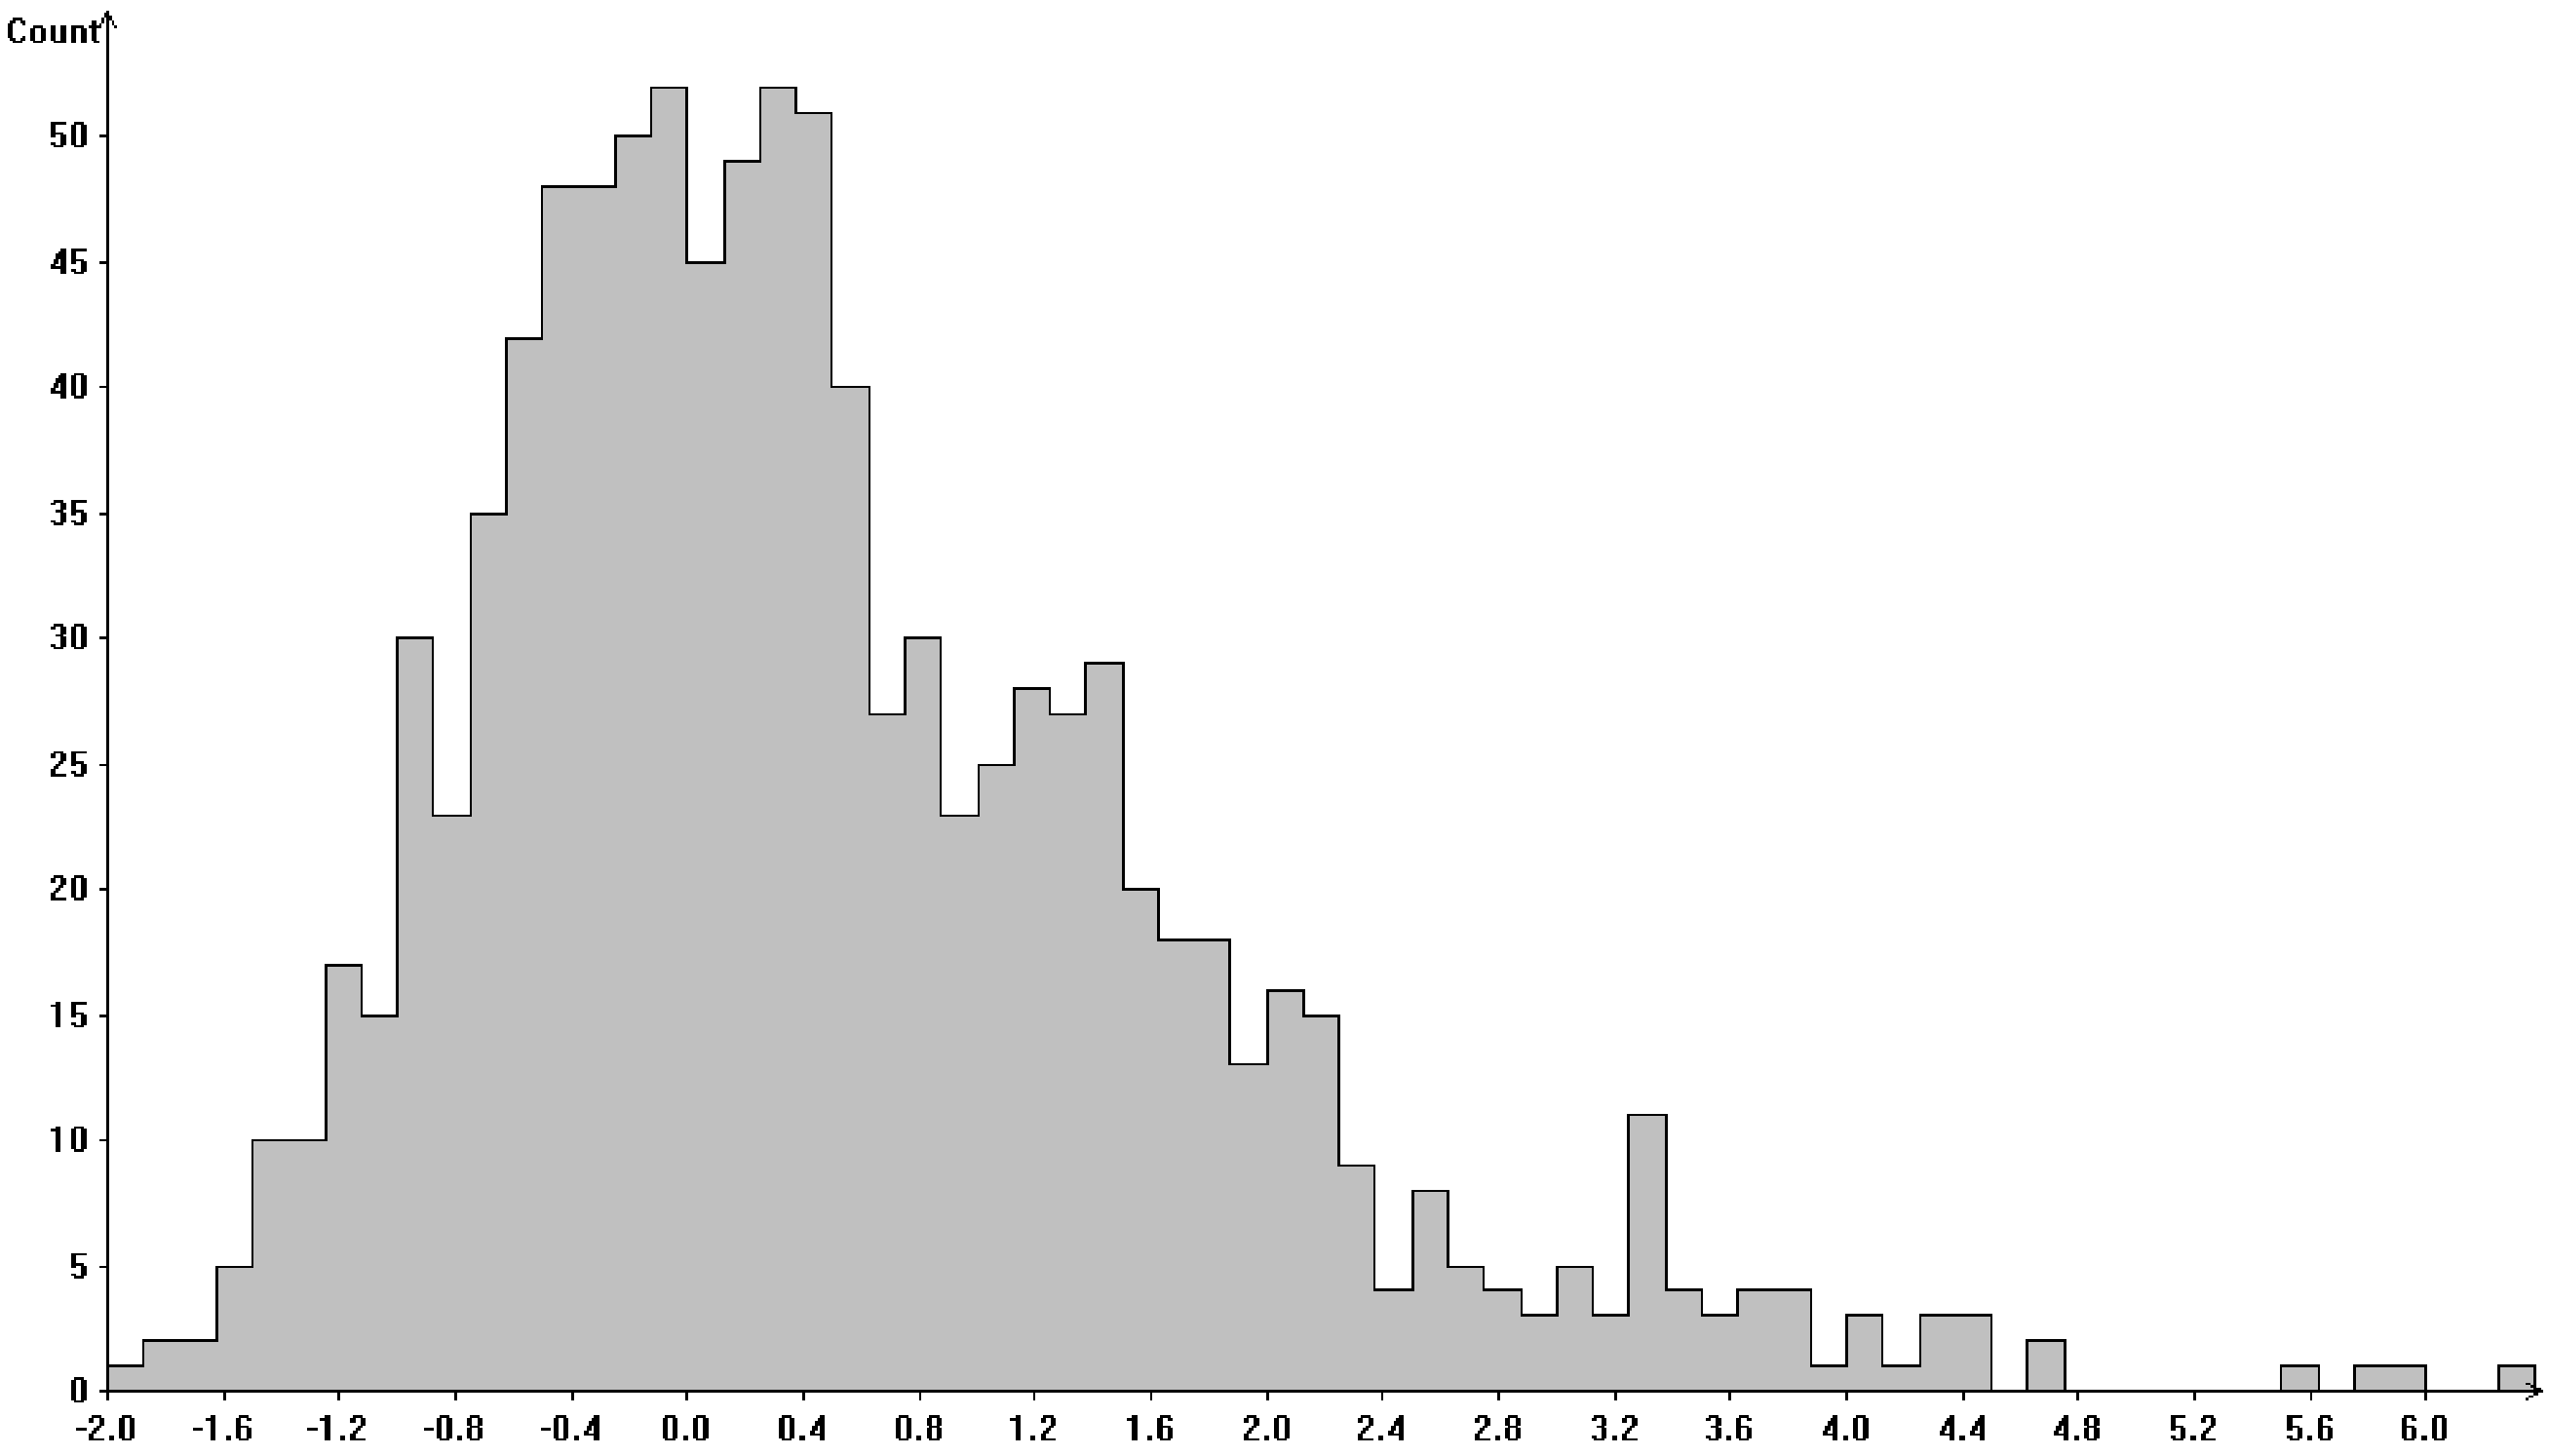
\includegraphics[width=12cm]{Figures/Histogram}
\caption{A typical histogram}\label{fig:histogram}
\end{figure}

A histogram is defined by three main parameters: $x_{\min}$, the
minimum of all values accumulated into the histogram, $w$, the bin
width and $n$, the number of bins. A bin is defined as an
interval. The $i\th$ bin of a histogram is the interval $\left[
x_{\min}+\left(i-1\right)w, x_{\min}+iw\right[$. The customary
convention is that the lower limit is included in the interval and
the higher limit excluded from the interval. The bin contents of a
histogram --- or histogram contents for short --- is the number of
times a value falls within each bin interval. Sometimes, a
histogram is defined by the minimum and maximum of the accumulated
values and the number of bins. The bin width is then computed as:
\begin{equation}
  w = {x_{\max} - x_{\min} \over n},
\end{equation}
where $x_{\max}$ is the maximum of the accumulated values.

In section \ref{sec:mlfhist} we shall need the error on the
contents of a histogram. In absence of any systematic
effects\footnote{A good example of systematic effect is when
values are computed from measurements made with an ADC. In this
case, the integer rounding of the ADC may interfere with the bin
sorting of the histogram.} the contents of each bin are
distributed according to a Poisson distribution. The standard
deviation of a Poisson distribution is the square root of the
average. The standard deviation is used as an estimator of the
error on the bin contents\footnote{This is not a contradiction to
what was said in section \ref{sec:moments}: the bin content is not
an average, but a counting}. If $n_i$ is the content of the $i\th$
bin of the histogram, the estimated error on the contents is
$\sqrt{n_i}$.

To obtain more information about the measured distribution, one
can also keep track of the number of values falling outside of the
histogram limits. The {\textsl underflow} of a histogram is defined as
the number of values falling below the minimum  of the accumulated
values. Similarly, the {\textsl overflow} of a histogram is defined as
the number of values falling on\footnote{This is different from
the definition of the underflow to be consistent with the fact
that the definition of a bin interval is open ended at the upper
limit.} or above the maximum of the accumulated values.

\subsection{Histograms --- General implementation}
\marginpar{Figure \ref{fig:statisticsclasses} with the box {\textbf
Histogram} grayed.} Our implementation of histogram also
accumulates the values into statistical moments. One can in
principle compute the statistical moments of the measured
distribution from the histogram contents. This determination,
however, depends strongly on the bin width, especially if the bin
width is large compared to the standard deviation. Thus, it is
preferable to use the original data when accumulating the
statistical moments. The net result is that a histogram has the
same polymorphic behavior as a statistical moment.

When defining a histogram, the histogram limits --- $x_{\min}$ and
$x_{\max}$ --- must be known in advance. This is not always
practical since it implies a first scan of the measurements to
determine the limits and a second scan to perform the accumulation
into the defined histogram. Thus, our implementation offers the
possibility of defining a histogram without predefined limits. In
this mode, the first values are cached into an array until a
sufficient number of data is available. When this happens, the
histogram limits are determined from the data and the cached
values are accumulated.

There are some cases when one would like to accumulates all the
values within the histogram limits. The proposed implementation
allows this by changing the histogram limits accordingly when a
new value falls outside of the current histogram limits. When a
histogram is accumulated in this mode the underflow and overflow
counts are always zero.

When the histogram limits are computed automatically, it can
happen that these limits have odd values. For example, if the
minimum value is 2.13456 and the maximum value is 5.1245,
selecting a number of bins of 50 would yield a bin width of
0.0597988. Of course such value for the bin width is quite
undesirable in practice. A similar thing can happen if the
application creating the histogram obtains the minimum and maximum
values from a computation or an automatic measuring device. To
avoid such silly parameters, our implementation computes a
reasonable limit and bin width by rounding the bin width to the
nearest reasonable scale at the order of magnitude\footnote{Let us
recall that the order of magnitude is the power of ten of a
number.} of the bin with. The possible scales are chosen to be
easily computed by a human. In our example, the order of magnitude
is $-2$. The bin width is then selected to be 0.075 and the
minimum and maximum are adjusted to be integral multiples of the
bin width enclosing the given limits. In our example, there are
$2.1$ and $5.175$ and the number of bins becomes 41 instead of 50.

\subsection{Histograms --- Smalltalk implementation}
\label{sec:shistogram} Listing \ref{ls:histogram} shows the
implementation of a histogram in Smalltalk. The following code
shows how to use the class {\texttt DhbHistogram} to accumulate
measurements into a histogram.
\begin{displaycode}{Smalltalk}

 | histogram valueStream |
 histogram := DhbHistogram new.
 [ valueStream atEnd ]
        whileFalse: [ histogram accumulate: valueStream next ].
\hfil {\texttt<\textsl printing or display of the histogram\texttt >}\hfil
\end{displaycode}

This example assumes that the measurement of the random variable
are obtained from a stream. The exact implementation of the stream
is not shown here.

After the declarative statements, the first executable statement
creates a new instance of the class {\texttt DhbHistogram} with the
default settings: automatic determination of the limits for 50
desired bins. The next two lines are the accumulation proper using
a {\texttt whileFalse:} construct and the general behavior of a
stream. This code is very similar to the code example presented in
section \ref{sec:smoments}. Extracting the parameters of the
distribution can also be performed from the histogram.

\noindent The next example shows how to declare a histogram with
given limits (2 and 7) and a desired number of bins of 50:
\begin{displaycode}{Smalltalk}
 | histogram valueStream |
 histogram := DhbHistogram new.
 histogram setRangeFrom: 2.0 to: 7.0 bins: 100.
\hfil {\texttt<\textsl the rest is identical to the previous example\texttt
>}\hfil
\end{displaycode}

\noindent The class {\texttt DhbHistogram} has the following instance
variables:
\begin{description}
  \item[\texttt minimum] the minimum of the accumulated values, that
  is $x_{\min}$,
  \item[\texttt binWidth] the bin width, that is $w$,
  \item[\texttt overflow] a counter to accumulate the overflow of the histogram,
  \item[\texttt underflow] a counter to accumulate the underflow of the histogram,
  \item[\texttt moments] an instance of the class {\texttt
  DhbFixedStatisticalMoments} to accumulate statistical moments up
  to the $4\th$ order (\cf section \ref{sec:srobustmoment}) with
  minimal rounding errors.
  \item[\texttt contents] the contents of the histogram, that is an
  array of integers,
  \item[\texttt freeExtent] a Boolean flag denoting whether the limits
  of the histogram can be adjusted to include all possible values,
  \item[\texttt cacheSize] the size of the cache allocated to collect
  values for an automatic determination of the histogram limits,
  \item[\texttt desiredNumberOfBins] the number of bins desired by the
  calling application.
\end{description}

Since there are many ways to declare a histogram, there is a
single creation method {\texttt new}, which calls in turn a single
standard initialization method {\texttt initialize}. In this mode. the
histogram is created with undefined limits --- that is, the first
accumulated values are cached until a sufficient number is
available for an automatic determination of the limits --- and a
default number of bins. The default number of bins is defined by
the class method {\texttt defaultNumberOfBins}.

\noindent Four methods allow to change the default initialization.

The method {\texttt setRangeFrom:to:bins:} allows the definition of
the parameters $x_{\min}$, $x_{\max}$ and $n$, respectively. The
method {\texttt setWidth:from:bins:} allows the definition of the
parameters $w$, $x_{\min}$ and $n$, respectively. In both cases,
the histogram limits and number of bins are adjusted to reasonable
values as explained at the end of section \ref{sec:histogram}.
These methods generate an error if the histogram is not cached, as
limits cannot be redefined while the histogram is accumulating.
The method {\texttt setDesiredNumberOfBins:} allows to overrule the
default number of bins. Finally, the method {\texttt freeExtent:}
takes a Boolean argument to define whether or not the limits must
be adjusted when an accumulated value falls outside of the
histogram limits. This method generates an error if any count has
been accumulated in the underflow or overflow.

The method {\texttt accumulate} is used to accumulate the values. If
the histogram is still cached --- that is when values are directly
accumulated into the cache for later determination of the limits
--- accumulation if delegated to the method {\texttt
accumulateInCache:}. In this mode, the instance variable {\texttt
contents} is an {\texttt OrderedCollection} collecting the values.
When the size of the collection is reaching the maximum size
allocated to the cache, limits are computed and the cache is
flushed. In direct accumulation mode, the bin index corresponding
to the value is computed. If the index is within the range, the
value is accumulated. Otherwise it is treated like an overflow or
an underflow. The method {\texttt processOverflows:for:} handles the
case where the accumulated values falls outside of the histogram
limits. If histogram limits cannot be adjusted it simply counts
the overflow or the underflow. Otherwise processing is delegated
to the methods {\texttt growsContents:}, {\texttt growsPositiveContents}
and {\texttt growsNegativeContents}, which adjust the histogram limits
according to the accumulated value.

The adjustment of the histogram limits to reasonable values is
performed by the method {\texttt adjustDimensionUpTo:}. This is made
when the limits are determined automatically. This method is also
used when the limits are specified using one of the initialization
methods.

There are many methods used to retrieve information from a
histogram. Enumerating them here would be too tedious. Method
names are explicit enough to get a rough idea of what each method
is doing; looking at the code should suffice for a detailed
understanding. The reader should just note that all methods
retrieving the parameters of the distribution, as discussed in
section \ref{sec:smoments}, are implemented by delegating the
method to the instance variable {\texttt moments}.

The iterator method {\texttt pointsAndErrorsDo:} is used for maximum
likelihood fit of a probability distribution. Smalltalk
implementation of maximum likelihood fit is discussed in section
\ref{sec:smlfhist}.

\begin{listing} Smalltalk implementation of histograms \label{ls:histogram}
$$\halign{ #\hfil&\quad#\hfil\cr {\sl Class}& {\Large\bf DhbHistogram}\cr
{\sl Subclass of }&{\tt Object}\cr\noalign{\vskip 1ex}

{\sl Instance variable names:}&\parbox[t]{4 in}{\tt  minimum binWidth overflow underflow moments contents freeExtent cacheSize desiredNumberOfBins }\cr\noalign{\vskip 1ex}}$$


Class methods
{\parskip 1ex\par\noindent}
{\bf defaultCacheSize}
\begin{verbatim}
    ^ 100
\end{verbatim}
{\bf defaultNumberOfBins}
\begin{verbatim}
    ^ 50
\end{verbatim}
{\bf integerScales}
\begin{verbatim}
   ^ self
\end{verbatim}

Instance methods
{\parskip 1ex\par\noindent}
{\bf accumulate:} {\tt aNumber}
\begin{verbatim}
    | bin |
    self isCached
        ifTrue: [ ^self accumulateInCache: aNumber ].
    bin := self binIndex: aNumber.
    ( bin between: 1 and: contents size)
        ifTrue: [ contents at: bin put: ( contents at: bin) + 1.
                     moments accumulate: aNumber.
                   ]
        ifFalse:[ self processOverflows: bin for: aNumber ].
\end{verbatim}
{\bf accumulateInCache:} {\tt aNumber}
\begin{verbatim}
    contents add: aNumber.
    contents size > cacheSize
        ifTrue: [ self flushCache ].
\end{verbatim}
{\bf adjustDimensionUpTo:} {\tt aNumber}
\begin{verbatim}
    | maximum |
    binWidth := self roundToScale: ( aNumber - minimum) / 
                                                  desiredNumberOfBins.
    minimum := ( minimum / binWidth) floor * binWidth.
    maximum := ( aNumber / binWidth) ceiling * binWidth.
    contents := Array new: ( ( maximum - minimum) / binWidth) 
                                                              ceiling.
    contents atAllPut: 0.
\end{verbatim}
{\bf average}
\begin{verbatim}
    ^ moments average
\end{verbatim}
{\bf binIndex:} {\tt aNumber}
\begin{verbatim}
    ^( ( aNumber - minimum) / binWidth) floor + 1
\end{verbatim}
{\bf binWidth}
\begin{verbatim}
    self isCached
        ifTrue: [ self flushCache].
    ^binWidth
\end{verbatim}
{\bf collectIntegralPoints:} {\tt aBlock}
\begin{verbatim}
    | answer bin lastContents integral norm x |
    self isCached
        ifTrue: [ self flushCache].
    answer := OrderedCollection new: ( contents size * 2 + 1).
    bin := self minimum.
    answer add: ( aBlock value: bin @ 0).
    integral := self underflow.
    norm := self totalCount.
    contents do:
        [ :each |
          integral := integral + each.
          x := integral / norm.
          answer add: ( aBlock value: bin @ x).
          bin := bin + binWidth.
          answer add: ( aBlock value: bin @ x).
        ].
    answer add: ( aBlock value: bin @ 0).
    ^ answer asArray
\end{verbatim}
{\bf collectPoints:} {\tt aBlock}
\begin{verbatim}
    | answer bin lastContents |
    self isCached
        ifTrue: [ self flushCache ].
    answer := OrderedCollection new: ( contents size * 2 + 1).
    bin := self minimum.
    answer add: (aBlock value: bin @ 0).
    contents do:
        [ :each |
          answer add: (aBlock value: bin @ each).
          bin := bin + binWidth.
          answer add: (aBlock value: bin @ each).
        ].
    answer add: (aBlock value: bin @ 0).
    ^ answer asArray
\end{verbatim}
{\bf count}
\begin{verbatim}
    ^ moments count
\end{verbatim}
{\bf countAt:} {\tt aNumber}
\begin{verbatim}
    | n |
    n := self binIndex: aNumber.
    ^ (n between: 1 and: contents size)
            ifTrue: [ contents at: n ]
            ifFalse: [ 0 ]
\end{verbatim}
{\bf countOverflows:} {\tt anInteger}
\begin{verbatim}
    anInteger > 0
        ifTrue: [ overflow := overflow + 1 ]
        ifFalse:[ underflow := underflow + 1 ].
\end{verbatim}
{\bf countsBetween:} {\tt aNumber1} {\bf and:} {\tt aNumber2}
\begin{verbatim}
    | n1 n2 answer |
    n1 := self binIndex: aNumber1.
    n2 := self binIndex: aNumber2.
    answer := ( contents at: n1) * ( ( binWidth * n1 + minimum) - 
                                                 aNumber1) / binWidth.
    n2 > contents size
        ifTrue: [ n2 := contents size + 1]
        ifFalse:[ answer := answer + ( ( contents at: n2) * ( 
      aNumber2 - ( binWidth * ( n2 - 1) + self maximum)) / binWidth)].
    ( n1 + 1) to: ( n2 - 1) do: [ :n | answer := answer + ( contents 
                                                              at: n)].
    ^ answer
\end{verbatim}
{\bf countsUpTo:} {\tt aNumber}
\begin{verbatim}
    | n answer |
    n := self binIndex: aNumber.
    n > contents size
        ifTrue: [ ^self count].
    answer := ( contents at: n) * ( aNumber - ( binWidth * ( n - 1) + 
                                            self minimum)) / binWidth.
    1 to: ( n - 1) do: [ :m | answer := answer + ( contents at: m)].
    ^ answer + underflow
\end{verbatim}
{\bf errorOnAverage}
\begin{verbatim}
    ^ moments errorOnAverage
\end{verbatim}
{\bf flushCache}
\begin{verbatim}
    | maximum values |
    minimum isNil
        ifTrue: [ minimum := contents isEmpty ifTrue: [ 0]
                                                                      
                                            ifFalse:[ contents first].
                   ].
    maximum := minimum.
    contents do:
        [ :each |
          each < minimum
            ifTrue: [ minimum := each]
            ifFalse:[ each > maximum
                            ifTrue: [ maximum := each].
                        ].
        ].
    maximum = minimum
        ifTrue: [ maximum := minimum + desiredNumberOfBins].
    values := contents.
    self adjustDimensionUpTo: maximum.
    values do: [ :each | self accumulate: each ].
\end{verbatim}
{\bf freeExtent:} {\tt aBoolean}
\begin{verbatim}
    ( underflow = 0 and: [ overflow = 0])
        ifFalse: [ self error: 'Histogram extent cannot be 
                                                          redefined'].
    freeExtent := aBoolean.
\end{verbatim}
{\bf growContents:} {\tt anInteger}
\begin{verbatim}
    anInteger > 0
        ifTrue: [ self growPositiveContents: anInteger ]
        ifFalse: [ self growNegativeContents: anInteger ].
\end{verbatim}
{\bf growNegativeContents:} {\tt anInteger}
\begin{verbatim}
    | n newSize newContents |
    n := 1 - anInteger.
    newSize := contents size + n.
    newContents := Array new: newSize.
    newContents
            at: 1 put: 1;
            replaceFrom: 2 to: n withObject: 0;
            replaceFrom: ( n + 1) to: newSize with: contents.
    contents := newContents.
    minimum := ( anInteger - 1) * binWidth + minimum.
\end{verbatim}
{\bf growPositiveContents:} {\tt anInteger}
\begin{verbatim}
    | n newContents |
    n := contents size.
    newContents := Array new: anInteger.
    newContents
            replaceFrom: 1 to: n with: contents;
            replaceFrom: ( n + 1) to: ( anInteger - 1) withObject: 0;
            at: anInteger put: 1.
    contents := newContents.
\end{verbatim}
{\bf initialize}
\begin{verbatim}
    freeExtent := false.
    cacheSize := self class defaultCacheSize.
    desiredNumberOfBins := self class defaultNumberOfBins.
    contents := OrderedCollection new: cacheSize.
    moments := DhbFixedStatisticalMoments new.
    overflow := 0.
    underflow := 0.
    ^ self
\end{verbatim}
{\bf inverseDistributionValue:} {\tt aNumber}
\begin{verbatim}
    | count x integral |
    count := self count * aNumber.
    x := self minimum.
    integral := 0.
    contents do:
        [ :each | | delta |
          delta := count - integral.
          each > delta
            ifTrue: [ ^self binWidth * delta / each + x].
          integral := integral + each.
          x := self binWidth + x.
        ].
    ^ self maximum
\end{verbatim}
{\bf isCached}
\begin{verbatim}
    ^ binWidth isNil
\end{verbatim}
{\bf isEmpty}
\begin{verbatim}
    ^ false
\end{verbatim}
{\bf kurtosis}
\begin{verbatim}
    ^ moments kurtosis
\end{verbatim}
{\bf lowBinLimitAt:} {\tt anInteger}
\begin{verbatim}
    ^ (anInteger - 1) * binWidth + minimum
\end{verbatim}
{\bf maximum}
\begin{verbatim}
    self isCached
        ifTrue: [ self flushCache ].
    ^ contents size * binWidth + minimum
\end{verbatim}
{\bf maximumCount}
\begin{verbatim}
    self isCached
        ifTrue: [ self flushCache ].
    ^contents inject: ( contents isEmpty ifTrue: [ 1] ifFalse:[ 
                                                      contents at: 1])
                    into: [ :max :each | max max: each]
\end{verbatim}
{\bf minimum}
\begin{verbatim}
    self isCached
        ifTrue: [ self flushCache ].
    ^ minimum
\end{verbatim}
{\bf overflow}
\begin{verbatim}
    ^ overflow
\end{verbatim}
{\bf processOverflows:} {\tt anInteger} {\bf for:} {\tt aNumber}
\begin{verbatim}
    freeExtent
        ifTrue: [ self growContents: anInteger.
                     moments accumulate: aNumber
                   ]
        ifFalse:[ self countOverflows: anInteger ].
\end{verbatim}
{\bf setDesiredNumberOfBins:} {\tt anInteger}
\begin{verbatim}
    anInteger > 0
        ifFalse:[ self error: 'Desired number of bins must be 
                                                           positive'].
    desiredNumberOfBins := anInteger.
\end{verbatim}
{\bf setRangeFrom:} {\tt aNumber1} {\bf to:} {\tt aNumber2} {\bf bins:} {\tt anInteger}
\begin{verbatim}
    self isCached
        ifFalse: [ self error: 'Histogram limits cannot be 
                                                          redefined'].
    minimum := aNumber1.
    self setDesiredNumberOfBins: anInteger;
           adjustDimensionUpTo: aNumber2.
\end{verbatim}
{\bf setWidth:} {\tt aNumber1} {\bf from:} {\tt aNumber2} {\bf bins:} {\tt anInteger}
\begin{verbatim}
    self isCached
        ifFalse: [ self error: 'Histogram limits cannot be 
                                                          redefined'].
    minimum := aNumber2.
    self setDesiredNumberOfBins: anInteger;
           adjustDimensionUpTo: ( aNumber1 * anInteger + aNumber2).
\end{verbatim}
{\bf skewness}
\begin{verbatim}
    ^ moments skewness
\end{verbatim}
{\bf standardDeviation}
\begin{verbatim}
    ^ moments standardDeviation
\end{verbatim}
{\bf totalCount}
\begin{verbatim}
    ^ moments count + underflow + overflow
\end{verbatim}
{\bf underflow}
\begin{verbatim}
    ^ underflow
\end{verbatim}
{\bf variance}
\begin{verbatim}
    ^ moments variance
\end{verbatim}


\end{listing}


\section{Random number generator}
\label{sec:random} When studying statistical processes on a
computer one often has to simulate the behavior of a random
variable\footnote{Another wide use for random number generators
are games.}. As we shall see in section \ref{sec:probdistr} it
suffice to implement a random generator for a uniform
distribution, that is a random variable whose probability density
function is constant over a given interval. Once such an
implementation is available, any probability distribution can be
simulated.

\rubrique{Linear congruential random generators} The most widely
used random number generators are linear congruential random
generators. Random numbers are obtained from the following series
\cite{Knuth2}:
\begin{equation}
\label{eq:crg}
  X_{n+1} = \left(aX_n+c\right) \mod m,
\end{equation}
where $m$ is called the modulus, $a$ the multiplier and $c$ the
increment. By definition, we have $0\leq X_n<m$ for all $n$. The
numbers $X_n$ are actually pseudo-random numbers since, for a
given modulus, multiplier and increment, the sequence of numbers
$X_1,\ldots,X_n$ is fully determined by the value $X_0$. The value
$X_0$ is called the seed of the series. In spite of its
reproducibility the generated series behaves very close to that of
random variable uniformly distributed between 0 and $m-1$. Then
the following variable:
\begin{equation}
  x_n = {X_n \over m},
\end{equation}
is a random rational number uniformly distributed between 0 and 1,
1 excluded.

In practice, the modulus, multiplier and increment must be chosen
quite carefully to achieve a good randomness of the series. Don
Knuth \cite{Knuth2} gives a series of criteria for choosing the
parameters of the random number generator. If the parameters are
correctly chosen, the seed $X_0$ can be assigned to any value.

\rubrique{Additive sequence generators} Another class of random
generators are additive sequence generators \cite{Knuth2}. The
series of pseudo-random numbers is generated as follows:
\begin{equation}
  X_n = \left(X_{n-l}+X_{n-k}\right) \mod m,
\end{equation}
where $m$ is the modulus as before and $l$ and $k$ are two indices
such that $l<k$. These indices must be selected carefully.
\cite{Knuth2} contains a table of suitable indices. The initial
series of numbers $X_1,\ldots,X_k$ can be any integers not all
even.

Generators based on additive sequences are ideal to generate
floating point numbers. If this case, the modulo operation on the
modulus is not needed. Instead, one simply checks whether or not
the newly generated number is larger than 1. Thus, the series
becomes:
\begin{equation}
\label{eq:addseqrandom}
  \begin{array}{lcl}
  y_n&=&x_{n-l}+x_{n-k},\\*[2ex]
  x_n&=&\left\{
    \begin{array}{ll}
    y_n&\mbox{\quad if $y_n<1$,}\\
    y_n-1&\mbox{\quad if $y_n\geq 1$,}\\
    \end{array}
  \right.
  \end{array}
\end{equation}
It is clear that the evaluation above is much faster than that of
equation \ref{eq:crg}. In practice, the additive sequence
generator is about 4 times faster. In addition, the length of the
sequence is larger than that of a  congruential random generator
with the same modulus.

In our implementation we have selected the pair of numbers
$\left(24,55\right)$ corresponding to the generator initially
discovered by G.J. Mitchell and D.P. Moore\cite{Knuth2}. The
corresponding sequence has a length of $2^{55}-1$. In our tests
(\cf below) we have found that the randomness of this generator is
at least as good as that of the congruential random generator. The
initial series $x_1,\ldots,x_{55}$ is obtained from the
congruential random generator.

In \cite{Knuth2} Don Knuth describes a wealth of test to
investigate the randomness of random number generators. Some of
these tests are also discussed in \cite{LawKel}. To study the
goodness of our proposed random generators, we have performed two
types of tests: a $\chi^2$ test and a correlation test.

The $\chi^2$ test is performed on a histogram, in which values
generated according to a probability distributions have been
accumulated. Then, a $\chi^2$ confidence level (\cf section
\ref{sec:chitest}) is calculated against the theoretical curve
computed using the histogram bin width, the number of generated
values and the parameters of the distribution. A confidence level
should be larger than $60\%$ indicates that the probability
distribution is correctly generated. When using distributions
requiring the generation of several random numbers to obtain one
value --- Normal distribution (2 values), gamma distribution (2
values) and beta distribution (4 values)
--- one can get a good confidence that short term
correlations\footnote{Pseudo random number generators have a
tendency to exhibit correlations in the series. That is, the
number $X_n$ can be correlated to the number $X_{n-k}$ for each
$n$ and a given $k$.} are not creating problems. The code for this
test is given in the code examples \ref{exs:chitest}. In this test the Mitchell-Moore
generator gives results similar to that of the congruential random
generator.

The correlation test is performed by computing the covariance
matrix (\cf section \ref{sec:covmatrix}) of vectors of given
dimension (between 5 and 10). The covariance matrix should be a
diagonal matrix with all diagonal elements equal to $1/12$, the
variance of a uniform distribution. Deviation from this
theoretical case should be small. Here longer correlations can be
investigated by varying the dimension of the generated vectors. In
this test too, the Mitchell-Moore generator gives results similar
to that of the congruential random generator.

\rubrique{Bit-pattern generators} The generators described above
are suitable to the generation of random values, but not for the
generation of random bit patterns \cite{Knuth2}, \cite{Press}. The
generation of random bit patterns can be achieved with generator
polynomials. Such polynomials are used in error correction codes
for their abilities to produce sequences of numbers with a maximum
number of different bits. For example the following polynomial
\begin{equation}
\label{eq:ranpolgen}
  G\left(x\right) = x^{16} + x^{12} +x^5 + 1,
\end{equation}
is a good generator for random patterns of 16 bits\footnote{\cf O.
Yamada, K. Yamazaki and D.H.Besset, {\em An Error-Correction
Scheme for an Optical Memory Card System}, 1990 International
Symposium on Information Theory and its Applications (ISITA'90),
Hawaii, USA, November 27-30, 1990.}. Of course, the evaluation of
equation \ref{eq:ranpolgen} does not require the computation of
the polynomial. The following algorithm can be used: {\parskip 0pt
\begin{enumerate}
  \item Set $X_{n+1}$ to $X_n$ shifted by one position to the left
  and truncated to 16 bits ($X_{n+1}=2X_n \mod 2^{16}$),
  \item If bit 15 (least significant bit being 0) of $X_n$ is set,
  set $X_{n+1}$ to the bit wise exclusive OR of $X_{n+1}$ with
  {\texttt 0x1021}.
\end{enumerate}}
\noindent Other polynomials are given in \cite{Press}.

Random bit patterns are usually used to simulate hardware
behavior. They are rarely used in statistical analysis. A concrete
implementation of a random bit pattern generator is left as an
exercise to the reader.

\subsection{Random number generator --- Smalltalk implementation}
\marginpar{Figure \ref{fig:statisticsclasses} with the boxes {\textbf
CongruentialRandomNumberGenerator} and {\textbf
MitchellMooreGenerator} grayed.} Listing \ref{ls:randomcong} shows
the implementation of a congruential random generator in
Smalltalk. Listing \ref{ls:randomseq} shows the implementation of
a additive sequence random generator in Smalltalk. Listing
\ref{ls:randomuse} shows usage of the generator for standard use.

\noindent The class {\texttt DhbCongruentialRandomNumberGenerator} has
three public methods:
\begin{description}
  \item[\texttt value] returns the next random number of the series,
  that is $X_n$, a number between $0$ and $m$,
  \item[\texttt floatValue] returns the next random floating number,
  that is the value $X_n / m$,
  \item[\texttt integerValue:] returns a random integer, whose values
  are between 0 and the specified argument.
\end{description}
When calling any of the above methods, the next random number of
the series is obtained using equation \ref{eq:crg}.

There are several ways of using a random number generator. If
there is no specific requirement the easiest approach is to use
the instance provided by default creation method ({\texttt new})
returning a \patstyle{singleton}. The next example shows how to
proceed assuming the application uses the values generated by the
random generator directly:
\begin{displaycode}{Smalltalk}
 | generator x |
 generator := DhbCongruentialRandomNumberGenerator new.
\hfil{\texttt <\textsl Here is where the generator is used\texttt
>}\hfil

 x := generator value.
\end{displaycode}

If one needs several series which must be separately reproducible,
one can assign several generators, one for each series. The
application can use predefined numbers for the seed of each
series. Here is a complete example assuming that the generated
numbers must be floating numbers.
\begin{displaycode}{Smalltalk}

 | generators seeds index x |

 {\texttt seeds := <\textsl an array containing the desired seeds\texttt >}

 generators := seeds collect:
           [ :each | DhbCongruentialRandomNumberGenerator seed: each].

\noindent\hskip 5ex{\texttt <\textsl Here is where the various generators
are used\texttt
>}\hfil \\
\hskip 5ex{\texttt <index \textsl is the index of the desired series\texttt
>}\hfil

 x := ( generators at: index) floatValue.
\end{displaycode}

In game applications, it is of course not desirable to have a
reproducible series. In this case, the easiest way is to use the
time in milliseconds as the seed of the series. This initial value
is sufficiently hard to reproduce to give the illusion of
randomness. Furthermore the randomness of the series guarantees
that two series generated at almost the same time are quite
different. Here is how to do it.
\begin{displaycode}{Smalltalk}

 | generator x |
 generator := DhbCongruentialRandomNumberGenerator
                        seed: Time millisecondClockValue.

\hfil{\texttt <\textsl Here is where the generator is used\texttt
>}\hfil

 x := (generator integerValue: 20) + 1.
\end{displaycode}

In this last example, the generated numbers are integers between 1
and 20.

\rubrique{Implementation} The class {\texttt
DhbCongruentialRandomNumberGenerator} has the following instance
variables:
\begin{description}
  \item[\texttt constant] the increment $c$,
  \item[\texttt modulus] the modulus $m$,
  \item[\texttt multiplicator] the multiplier $a$ and
  \item[\texttt seed] the last generated number $X_{n-1}$.
\end{description}
There are three instance creation methods. The method {\texttt new}
returns a \patstyle{singleton} instance containing parameters from
\cite{Knuth2}. The method {\texttt seed:} allows one to create an
instance to generate a series of random number starting at a given
seed. Finally the method {\texttt constant:multiplicator:modulus:}
creates a congruential random number generator based on supplied
parameters. Readers tempted to use this method are strongly
advised to read \cite{Knuth2} and the references therein
thoroughly. Then, they should perform tests to verify that their
parameters are indeed producing a series with acceptable
randomness.

The modulus of the standard parameters has 32 bits. In the
Smalltalk implementation, however, the evaluation of equation
\ref{eq:crg} generates integers larger than 32 bits. As a result,
the generation of the random numbers is somewhat slow, as it is
using multiple precision integers. Using floating
number\footnote{The author is grateful to Dave N. Smith of IBM for
this useful tip.} does not disturb the evaluation of equation
\ref{eq:crg} and is significantly faster since floating point
evaluation is performed on the hardware. The generation of random
numbers using floating point parameters is about 3 times faster
than with integer parameters. This can easily be verified by the
reader.

\begin{listing} Smalltalk implementation of congruential random number generators
\label{ls:randomcong}
$$\halign{ #\hfil&\quad#\hfil\cr {\sl Class}& {\Large\bf DhbCongruentialRandomNumberGenerator}\cr
{\sl Subclass of }&{\tt Object}\cr\noalign{\vskip 1ex}

{\sl Instance variable names:}&\parbox[t]{4 in}{\tt  constant modulus multiplicator seed }\cr\noalign{\vskip 1ex}
{\sl Class variable names:}&\parbox[t]{4 in}{\tt  UniqueInstance }\cr\noalign{\vskip 1ex}}$$


Class methods
{\parskip 1ex\par\noindent}
{\bf constant:} {\tt aNumber1} {\bf multiplicator:} {\tt aNumber2} {\bf modulus:} {\tt aNumber3}
\begin{verbatim}
    ^ super new 
        initialize: aNumber1
        multiplicator: aNumber2
        modulus: aNumber3

\end{verbatim}
{\bf new}
\begin{verbatim}
    UniqueInstance isNil
        ifTrue: [ UniqueInstance := super new initialize.
                     UniqueInstance setSeed: 1 ].
    ^ UniqueInstance
\end{verbatim}
{\bf seed:} {\tt aNumber}
\begin{verbatim}
    ^ super new initialize; setSeed: aNumber; yourself
\end{verbatim}

Instance methods
{\parskip 1ex\par\noindent}
{\bf floatValue}
\begin{verbatim}
    ^ self value asFloat / modulus
\end{verbatim}
{\bf initialize}
\begin{verbatim}
    self initialize: 2718281829.0 multiplicator: 3141592653.0 
                                                modulus: 4294967296.0.
\end{verbatim}
{\bf initialize:} {\tt aNumber1} {\bf multiplicator:} {\tt aNumber2} {\bf modulus:} {\tt aNumber3}
\begin{verbatim}
    constant := aNumber1.
    modulus := aNumber2.
    multiplicator := aNumber3.
    self setSeed: 1.
\end{verbatim}
{\bf integerValue:} {\tt anInteger}
\begin{verbatim}
    ^ (self value \\ ( anInteger * 1000)) // 1000
\end{verbatim}
{\bf setSeed:} {\tt aNumber}
\begin{verbatim}
    seed := aNumber.
\end{verbatim}
{\bf value}
\begin{verbatim}
    seed := (seed * multiplicator + constant) \\ modulus.
    ^ seed
\end{verbatim}


\end{listing}

\noindent The class {\texttt DhbMitchellMooreGenerator} implements a
random number generator with additive sequence. It has two public
methods:
\begin{description}
  \item[\texttt floatValue] returns the next random floating number,
  that is the value $x_n$,
  \item[\texttt integerValue:] returns a random integer, whose values
  are between 0 and the specified argument.
\end{description}
When calling any of the above methods, the next random number of
the series is obtained using equation \ref{eq:addseqrandom}. The
series of generated numbers are all floating points.

The creation methods {\texttt new} and {\texttt seed:} are used exactly as
the corresponding methods of the class {\texttt
DhbCongruentialRandomNumberGenerator}. Please refer to the code
examples \ref{codex:crgdefault} and \ref{codex:crgseeded}. Both
methods use the congruential random number generator to generate
the initial series of numbers $x_1,\ldots,x_{55}$. The class
method {\texttt constants:lowIndex:} offers a way to define the
numbers $k$ and $l$ as well as the initial series of numbers. The
reader wishing to use this method should consult the table of {\textsl
good} indices $k$ and $l$ in \cite{Knuth2}.

\begin{listing} Smalltalk implementation of an additive sequence random number generator
\label{ls:randomseq}
$$\halign{ #\hfil&\quad#\hfil\cr {\sl Class}& {\Large\bf DhbMitchellMooreGenerator}\cr
{\sl Subclass of }&{\tt Object}\cr\noalign{\vskip 1ex}

{\sl Instance variable names:}&\parbox[t]{4 in}{\tt  randoms lowIndex highIndex }\cr\noalign{\vskip 1ex}
{\sl Class variable names:}&\parbox[t]{4 in}{\tt  UniqueInstance }\cr\noalign{\vskip 1ex}}$$


Class methods
{\parskip 1ex\par\noindent}
{\bf constants:} {\tt anArray} {\bf lowIndex:} {\tt anInteger}
\begin{verbatim}
    ^super new initialize: anArray lowIndex: anInteger

\end{verbatim}
{\bf default}
\begin{verbatim}
    | congruentialGenerator |
    congruentialGenerator := DhbCongruentialRandomNumberGenerator 
                                                                  new.
    ^ self generateSeeds: congruentialGenerator
\end{verbatim}
{\bf generateSeeds:} {\tt congruentialGenerator}
\begin{verbatim}

\end{verbatim}
{\bf new}
\begin{verbatim}
    UniqueInstance isNil
        ifTrue: [ UniqueInstance := self default].
    ^ UniqueInstance
\end{verbatim}
{\bf seed:} {\tt anInteger}
\begin{verbatim}
    | congruentialGenerator |
    congruentialGenerator := DhbCongruentialRandomNumberGenerator 
                                                      seed: anInteger.
    ^self generateSeeds: congruentialGenerator
\end{verbatim}

Instance methods
{\parskip 1ex\par\noindent}
{\bf floatValue}
\begin{verbatim}
    | x |
    x := (randoms at: lowIndex) + (randoms at: highIndex).
    x < 1.0 ifFalse: [x := x - 1.0].
    randoms at: highIndex put: x.
    highIndex := highIndex + 1.
    highIndex > randoms size ifTrue: [highIndex := 1].
    lowIndex := lowIndex + 1.
    lowIndex > randoms size ifTrue: [lowIndex := 1].
    ^ x

\end{verbatim}
{\bf initialize:} {\tt anArray} {\bf lowIndex:} {\tt anInteger}
\begin{verbatim}
    randoms := anArray.
    lowIndex := anInteger.
    highIndex := randoms size.
    ^ self
\end{verbatim}
{\bf integerValue:} {\tt anInteger}
\begin{verbatim}
    ^ (self floatValue * anInteger) truncated
\end{verbatim}


\end{listing}

For simple simulation, one wishes to generate a random number ---
floating or integer --- within certain limits. Here are
convenience methods implemented for the class {\texttt Number} and
{\texttt Integer}. These methods frees the user from keeping track of
the instance of the random number generator. For example, the
following Smalltalk expression
\begin{quote}
\begin{verbatim}
 50 random
\end{verbatim}
\end{quote}
\noindent generates an integer random number between 0 and 49
included. Similarly the following Smalltalk expression
\begin{quote}
\begin{verbatim}
 2.45 random
\end{verbatim}
\end{quote}
\noindent generates a floating random number between 0 and $2.45$
excluded. Finally the following Smalltalk expression
\begin{quote}
\begin{verbatim}
 Number random
\end{verbatim}
\end{quote}
\noindent generates a floating random number between 0 and 1
excluded.
\begin{listing} Smalltalk implementation of random number generators
\label{ls:randomuse}
$$\halign{ #\hfil&\quad#\hfil\cr {\sl Class}& {\Large\bf Integer}\cr
{\sl Subclass of }&{\tt Number}\cr\noalign{\vskip 1ex}
}$$


Instance methods
{\parskip 1ex\par\noindent}
{\bf random}
\begin{verbatim}
    ^DhbMitchellMooreGenerator new integerValue: self
\end{verbatim}


$$\halign{ #\hfil&\quad#\hfil\cr {\sl Class}& {\Large\bf Number}\cr
{\sl Subclass of }&{\tt Magnitude}\cr\noalign{\vskip 1ex}
}$$


Class methods
{\parskip 1ex\par\noindent}
{\bf random}
\begin{verbatim}
    ^ DhbMitchellMooreGenerator new floatValue
\end{verbatim}



Instance methods
{\parskip 1ex\par\noindent}
{\bf random}
\begin{verbatim}
    ^ self class random * self
\end{verbatim}


\end{listing}

\section{Probability distributions}
\label{sec:probdistr}A probability density function defines the
probability of finding a continuous random variable within an
infinitesimal interval. More precisely, the probability density
function $P\left(x\right)$ gives the probability for a random
variable to take a value lying in the interval
$\left[x,x+dx\right[$. A probability density function is a special
case of a one variable function described in section
\ref{sec:function}.

The moment of $k^{\mathop{\textrm th}}$ order for a probability
density function $P\left(x\right)$ is defined by:
\begin{equation}
\label{eq:probdensity}
  M_k=\int x^k P\left(x\right) dx,
\end{equation}
where the range of the integral is taken over the range where the
function $P\left(x\right)$ is defined. By definition probability
density functions are normalized, that is, $M_0$ is equal to 1.

As for statistical moments, one defines the mean or average of the
distribution as:
\begin{equation}
  \mu=M_1=\int x P\left(x\right) dx.
\end{equation}
Then the central moment of $k^{\mathop{\textrm th}}$ order is defined
by:
\begin{equation}
  m_k=\int \left(x-\mu\right)^k P\left(x\right) dx.
\end{equation}
In particular the variance is defined as $m_2$, the central moment
of second order. The standard deviation, $\sigma$, is the square
root of $m_2$. The skewness and kurtosis\footnote{In old
references the kurtosis, as defined here, is called excess; then,
the kurtosis is defined as the square of the excess;
\cite{AbrSteg} \eg.} of a probability density function are
respectively defined as:
\begin{equation}
  \omega={\displaystyle m_3 \over\displaystyle {\root 3/2 \of m_2}}
  ={\displaystyle m_3 \over\displaystyle \sigma^3}\mbox{\quad and}
\end{equation}
\begin{equation}
  \kappa={\displaystyle m_4 \over\displaystyle m_2^2}-3
  ={\displaystyle m_4 \over\displaystyle \sigma^4}-3.
\end{equation}

The distribution function, also called acceptance function or
repartition function, is defined as the probability for the random
variable to have a value smaller or equal to a given value. For a
probability density function defined over all real numbers we
have:
\begin{equation}
\label{eq:defdistr}
  F\left(t\right)=\prob\left(x<t\right)=\int_{-\infty}^t P\left(x\right)
  dx.
\end{equation}
If the probability density function $P\left(x\right)$ is defined
over a restricted range, the lower limit of the integral in
equation \ref{eq:defdistr} must be changed accordingly. For
example, if the probability density function is defined for $x\geq
x_{\min}$ , the distribution function is given by:
\begin{equation}
\label{eq:defdistrmin}
  F\left(t\right)=\prob\left(x<t\right)=\int_{x_{\min}}^t P\left(x\right)
  dx.
\end{equation}
Instead of the distribution function,  the name centile is
sometimes used to refer to the value of the distribution function
expressed in percent. This kind of terminology is frequently used
in medical and natural science publications. For example, a value
$x$ is said to be at the $10^{\mathop{\textrm th}}$ centile if
$F\left(t\right)=1/10$; in other words, there is a ten-percent
chance of observing a value less than or equal to $t$\footnote{A
centile can also be quoted for a value relative to a set of
observed values.}.

The interval acceptance function measures the probability for the
random variable to have a value between two given values. That is
\begin{equation}
\label{eq:defacceptint}
  F\left(x_1,x_2\right)=\prob\left(x_1\le x<x_2\right)
  =\int_{x_1}^{x_2} P\left(x\right)dx,
\end{equation}
\begin{equation}
\label{eq:defacceptdiff}
  F\left(x_1,x_2\right)=F\left(x_2\right)-F\left(x_1\right).
\end{equation}
If the integral of equation \ref{eq:defdistr} can be resolved into
a closed expression or if it has a numerical approximation, the
evaluation of the interval acceptance function is made using
equation \ref{eq:defacceptdiff}. Otherwise the interval acceptance
function must be evaluated using Romberg integration (\cf section
\ref{sec:romberg}) applied to equation \ref{eq:defacceptint}.

The inverse of the repartition function is frequently used. For
example, in order to determine an acceptance threshold in a
decision process, one needs to determine the variable $t$ such
that the repartition function is equal to a given value $p$. In
other words, $t=F^{-1}\left(p\right)$. For example, the threshold
of a coin detection mechanism to only reject $99.9\%$ of the good
coins is $F^{-1}\left(0.999\right)$. If the distribution function
is not invertible, one can solve this equation using the Newton's
zero-finding method exposed in section \ref{sec:snewton}. Newton's
zero-finding method is especially handy since the derivative of
the function is known: it is the probability density function.
Since $F\left(x\right)$ is strictly monotonous between 0 and 1 a
unique solution is guaranteed for any $p$ within the open interval
$\left]0,1\right[$. The initial value for the search can be
obtained from Markov's inequality \cite{CorLeiRiv}, which can be
written in the form:
\begin{equation}
  t\le {\displaystyle \mu \over\displaystyle 1-F\left(t\right)}
\end{equation}
If no closed expression exists for the distribution function (it
is determined using numerical integration \eg) the computation of
the inverse value is best obtained by interpolating the inverse
function over a set of by tabulated values (\cf section
\ref{ch:interpolation}).

The inverse of the distribution function is also used to generate
a random variable distributed according to the distribution.
Namely, if $r$ is a random variable uniformly distributed between
0 and 1, then the variable $x=F^{-1}\left(r\right)$ is a random
variable distributed according to the distribution whose
distribution function is $F\left(x\right)$. In practice this
method can only be used if a closed expression exists for the
distribution function, otherwise the function must be tabulated
and Newton interpolation can be used on the inverse function (\cf
section \ref{sec:newtoninterpol}). For most known distributions,
however, special algorithms exist to generate random values
distributed according to a given distribution. Such algorithms are
described in \cite{LawKel}. They are not discussed here, but the
code is included in each implementation of the specific
probability distribution.

In the rest of this chapter we shall present the distributions
used in this book. Other important distributions are presented in
appendix \ref{ch:distributions}.

\subsection{Probability distributions --- Smalltalk implementation}
\marginpar{Figure \ref{fig:statisticsclasses} with the boxes {\textbf
ProbabilityDensity} and {\textbf
ProbabilityDensityWithUnknownDistribution} grayed.} Table
\ref{tb:distrgenimpl} shows the description of the public methods
of the implementation.
\begin{table}[h]
  \centering
  \caption{Public methods for probability density functions}
  \label{tb:distrgenimpl}
\vspace{1 ex}
\begin{tabular}{|l | l |} \hline
  Description & \hfil Smalltalk \\ \hline
  $P\left(x\right)$ & {\texttt value:} \\
  $F\left(x\right)$ & {\texttt distributionValue:} \\
  $F\left(x_1,x_2\right)$ & {\texttt acceptanceBetween:and:} \\
  $F^{-1}\left(x\right)$ & {\texttt inverseDistributionValue:} \\
  $x^{\dag}$ & {\texttt random} \\
  \hline
  $\bar{x}$ & {\texttt average} \\
  $\sigma^2$ & {\texttt variance} \\
  $\sigma$ & {\texttt standardDeviation} \\
  skewness & {\texttt skewness} \\
  kurtosis & {\texttt kurtosis} \\
  \hline
\end{tabular}
$\dag$ $x$ represents the random variable itself. In other words,
the method {\texttt random} returns a random value distributed
according to the distribution.
\end{table}

Depending on the distribution, closed expressions for the variance
or the standard deviation exist. Here general methods are supplied
to compute one from the other. Subclasses must implement at least
one of them; otherwise a stack overflow will result.

Methods to compute skewness and kurtosis are supplied, but return
{\texttt nil} in Smalltalk. A very general
implementation could have used explicit integration. The
integration interval, however, maybe infinite and a general
integration strategy cannot easily be supplied. Subclasses are
expected to implement both methods.

As we have quoted earlier a probability density function is a
function, as defined in section \ref{sec:function}. Since the
distribution function is also a function, a \patstyle{Adapter}
must be provided to create a function (as defined in section
\ref{sec:function}) for the distribution function.

Listing \ref{ls:probdistr} shows the implementation of a general
probability density distribution in Smalltalk. The class {\texttt
DhbProbabilityDensity} is an abstract implementation. Concrete
implementation of probability density distributions are subclass
of it.

The method {\texttt distributionValue:} returning the value of the
distribution function must be implemented by the subclass. The
method to compute the interval acceptance functions is using
equation \ref{eq:defacceptdiff} .

The inverse acceptance function is defined with two methods, one
public and one private. The public method verifies the range of
the argument, which must lie between 0 and 1. The private method
uses the class {\texttt DhbNewtonZeroFinder} discussed in section
\ref{sec:snewton}. The derivative needed by the Newton zero finder
is the probability density function itself since, by definition,
it is the derivative of the acceptance function (\cf equation
\ref{eq:defdistr}).

Finally the class creation method {\texttt fromHistogram:} creates a
new instance of a probability distribution with parameters derived
using a quick approximation from the data accumulated into the
supplied histogram; the derivation assumes that the accumulated
data are distributed according to the distribution. This method is
used to compute suitable starting values for least square or
maximum likelihood fits (\cf chapter \ref{ch:estimation}). The
convention is that this methods returns {\texttt nil} if the
parameters cannot be obtained. Thus, returning {\texttt nil} is the
default behavior for the superclass since this method is specific
to each distribution. The estimation of the parameters is usually
made using the statistical moments of the histogram and comparing
them to the analytical expression of the distribution's parameter.

\begin{listing} Smalltalk implementation of a probability distribution
\label{ls:probdistr}
$$\halign{ #\hfil&\quad#\hfil\cr {\sl Class}& {\Large\bf DhbProbabilityDensity}\cr
{\sl Subclass of }&{\tt Object}\cr\noalign{\vskip 1ex}
}$$


Class methods
{\parskip 1ex\par\noindent}
{\bf distributionName}
\begin{verbatim}
    ^ 'Unknown distribution'
\end{verbatim}
{\bf fromHistogram:} {\tt aHistogram}
\begin{verbatim}
    ^ nil
\end{verbatim}

Instance methods
{\parskip 1ex\par\noindent}
{\bf acceptanceBetween:} {\tt aNumber1} {\bf and:} {\tt aNumber2}
\begin{verbatim}
    ^ (self distributionValue: aNumber2) - (self distributionValue: 
                                                             aNumber1)
\end{verbatim}
{\bf approximatedValueAndGradient:} {\tt aNumber}
\begin{verbatim}
    | delta parameters dp gradient n |
    parameters := self parameters.
    n := parameters size.
    dp := self value: aNumber.
    delta := Array new: n.
    delta atAllPut: 0.
    gradient := DhbVector new: n.
    1 to: n do:
        [ :k |
          delta at: k put: ( parameters at: k) * 0.0001.
          self changeParametersBy: delta.
          gradient at: k put: ( ( ( self value: aNumber) - dp) / ( 
                                                        delta at: k)).
          delta at: k put: ( delta at: k ) negated.
          k > 1
            ifTrue: [ delta at: ( k - 1) put: 0].
        ].
    self changeParametersBy: delta.
    ^Array with: dp with: gradient
\end{verbatim}
{\bf average}
\begin{verbatim}
    self subclassResponsibility.
\end{verbatim}
{\bf distributionFunction}
\begin{verbatim}
    ^ DhbProbabilityDistributionFunction density: self
\end{verbatim}
{\bf distributionValue:} {\tt aNumber}
\begin{verbatim}
    ^ self subclassResponsibility

\end{verbatim}
{\bf inverseDistributionValue:} {\tt aNumber}
\begin{verbatim}
    ^ (aNumber between: 0 and: 1)
            ifTrue: [ self privateInverseDistributionValue: aNumber]
            ifFalse:[ self error: 'Illegal argument for inverse 
                                                  distribution value']
\end{verbatim}
{\bf kurtosis}
\begin{verbatim}
    ^ nil
\end{verbatim}
{\bf parameters}
\begin{verbatim}
    ^ self subclassResponsibility
\end{verbatim}
{\bf printOn:} {\tt aStream}
\begin{verbatim}
    aStream nextPutAll: self class distributionName.
    self parameters ifNotNil: [ :params | | first |
        first := true.
        aStream nextPut: $(.
        params do:
            [ :each |
            first ifTrue: [ first := false]
                    ifFalse:[ aStream nextPut: $,].
            aStream space.
            each printOn: aStream.
            ].
        aStream nextPut: $).
        ].
\end{verbatim}
{\bf privateInverseDistributionValue:} {\tt aNumber}
\begin{verbatim}
    ^(DhbNewtonZeroFinder function: [ :x | ( self distributionValue: 
                                       x) - aNumber] derivative: self)
        initialValue: self average / (1 - aNumber); evaluate
\end{verbatim}
{\bf random}
\begin{verbatim}
    ^ self privateInverseDistributionValue: DhbMitchellMooreGenerator 
                                                        new floatValue
\end{verbatim}
{\bf skewness}
\begin{verbatim}
    ^ nil
\end{verbatim}
{\bf standardDeviation}
\begin{verbatim}
    ^ self variance sqrt
\end{verbatim}
{\bf value:} {\tt aNumber}
\begin{verbatim}
    self subclassResponsibility.
\end{verbatim}
{\bf valueAndGradient:} {\tt aNumber}
\begin{verbatim}
    ^ self approximatedValueAndGradient: aNumber
\end{verbatim}
{\bf variance}
\begin{verbatim}
    ^ self standardDeviation squared
\end{verbatim}


\end{listing}

The class {\texttt DhbProbabilityDensityWithUnknownDistribution} is
the abstract class for probability distribution having neither an
analytical expression nor a numerical approximation for the
distribution function.

Therefore, methods computing the acceptance function ({\texttt
distributionValue:}) and interval acceptance ({\texttt
acceptanceBetween:and:}) are using equations \ref{eq:defdistr} and
\ref{eq:defacceptint} respectively, using the class {\texttt
DhbRombergIntegrator} discussed in section \ref{sec:sromberg}. The
lower limit of the integral for the distribution function ---
$x_{\min}$ of equation \ref{eq:defdistrmin} --- is defined by the
method {\texttt lowestValue}. Since the majority of the probability
density distributions are defined for non-negative numbers, this
method returns 0. If the supplied default is not appropriate, the
method {\texttt lowestValue} must be redefined by the subclass.

\begin{listing} Smalltalk implementation of a probability distribution with unknown
distribution function\label{ls:probunkdistr}
$$\halign{ #\hfil&\quad#\hfil\cr {\sl Class}& {\Large\bf DhbProbabilityDensityWithUnknownDistribution}\cr
{\sl Subclass of }&{\tt DhbProbabilityDensity}\cr\noalign{\vskip 1ex}
}$$

Instance methods
{\parskip 1ex\par\noindent}
{\bf acceptanceBetween:} {\tt aNumber1} {\bf and:} {\tt aNumber2}
\begin{verbatim}
    ^ (DhbRombergIntegrator new: self from: aNumber1 to: aNumber2) 
                                                              evaluate
\end{verbatim}
{\bf distributionValue:} {\tt aNumber}
\begin{verbatim}
    ^ (DhbRombergIntegrator new: self from: self lowestValue to: 
                                                     aNumber) evaluate
\end{verbatim}
{\bf lowestValue}
\begin{verbatim}
    ^ 0
\end{verbatim}


\end{listing}

Listing \ref{ls:probdistrfun} shows the implementation of the
\patstyle{Adapter} for the distribution function. The class {\texttt
DhbProbabilityDistributionFunction} has a single instance variable
containing the corresponding probability density function. The
creation method {\texttt density:} takes an instance of class {\texttt
DhbProbabilityDensity} as argument.

\begin{listing} Smalltalk implementation of a probability distribution function
\label{ls:probdistrfun}
$$\halign{ #\hfil&\quad#\hfil\cr {\sl Class}& {\Large\bf DhbProbabilityDistributionFunction}\cr
{\sl Subclass of }&{\tt Object}\cr\noalign{\vskip 1ex}

{\sl Instance variable names:}&\parbox[t]{4 in}{\tt  probabilityDensity }\cr\noalign{\vskip 1ex}}$$


Class methods
{\parskip 1ex\par\noindent}
{\bf density:} {\tt aProbabilityDensity}
\begin{verbatim}
    ^ self new initialize: aProbabilityDensity
\end{verbatim}

Instance methods
{\parskip 1ex\par\noindent}
{\bf initialize:} {\tt aProbabilityDensity}
\begin{verbatim}
    probabilityDensity := aProbabilityDensity.
    ^ self
\end{verbatim}
{\bf value:} {\tt aNumber}
\begin{verbatim}
    ^ probabilityDensity distributionValue: aNumber
\end{verbatim}


\end{listing}


\section{Normal distribution}
\label{sec:normdist} The normal distribution is the most important
probability distribution. Most other distributions tend toward it
when some of their parameters become large. Experimental data
subjected only\footnote{The presence of systematic errors is a
notable exception to this rule.} to measurement fluctuation
usually follow a normal distribution.

\noindent Table \ref{tb:normdist} shows the properties of the
normal distribution.
\begin{table}[h]
  \centering
  \caption{Properties of the Normal distribution}\label{tb:normdist}
\vspace{1 ex}
\begin{tabular}{|l|c|} \hline \vbox to 3ex{}
  Range of random variable & $\left]-\infty,+\infty\right[$\\
  *[1ex] \hline \vbox to 4ex{}
  Probability density function & $\displaystyle P\left(x\right)={1\over \sqrt{2\pi\sigma^2}}e^{-{\left(x-\mu\right)^2\over 2\sigma^2}}$ \\*[2ex]  \hline
  \vbox to 3ex{} Parameters & $-\infty<\mu<+\infty$ \\
  &$0<\sigma<+\infty$ \\*[1ex]  \hline \vbox to 4ex{}
  Distribution function & $\displaystyle F\left(x\right)=\erf\left({x-\mu\over\sigma}\right)$ \\
  &(\cf section \ref{sec:errorFunction}) \\*[1ex]  \hline
  \vbox to 3ex{}Average & $\mu$ \\*[1ex] \hline
  \vbox to 3ex{}Variance & $\sigma^2$ \\*[1ex] \hline
  \vbox to 3ex{}Skewness & $0$ \\*[1ex] \hline
  \vbox to 3ex{}Kurtosis & $0$ \\*[1ex] \hline
\end{tabular}
\end{table}
Figure \ref{fig:normDistr} shows the well-known bell shape of the
normal distribution for various values of the parameters. The
reader can see that the peak of the distribution is always located
at $\mu$ and that the width of the bell curve is proportional to
$\sigma$.
\begin{figure}
\centering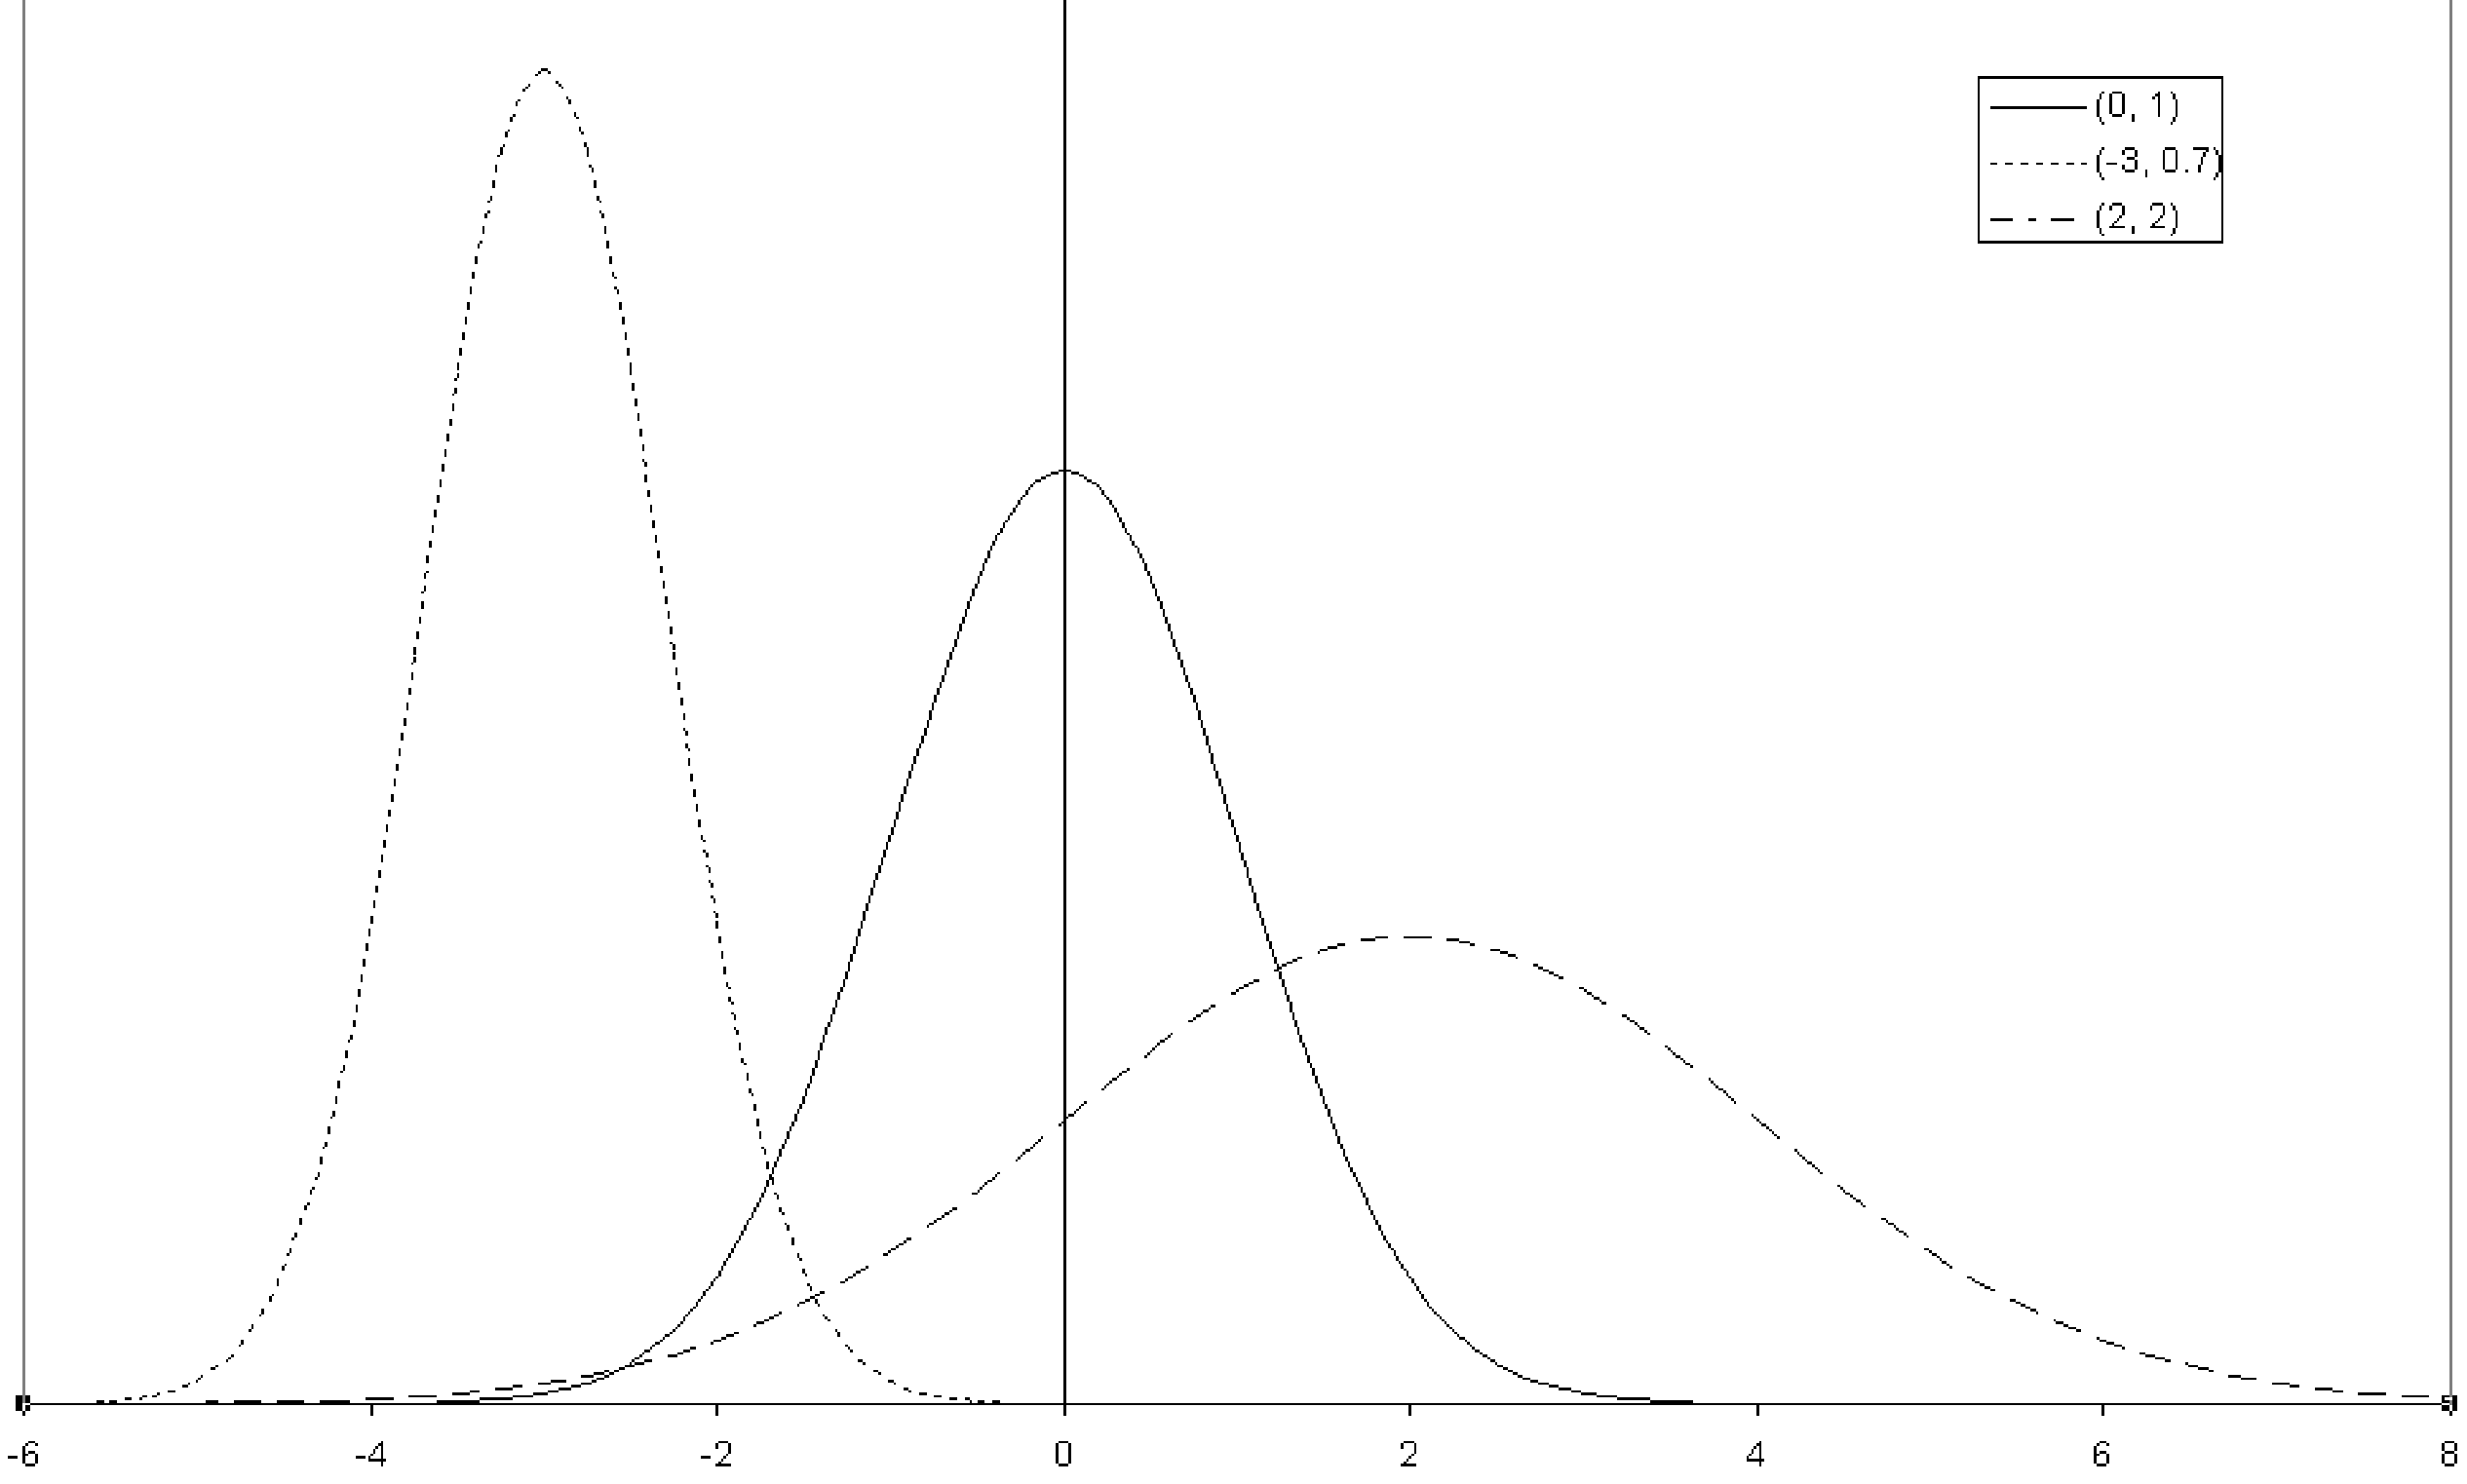
\includegraphics[width=12cm]{Figures/NormalDistribution}
\caption{Normal distribution for various values of the parameters
}\label{fig:normDistr}
\end{figure}

\subsection{Normal distribution --- Smalltalk implementation}
\marginpar{Figure \ref{fig:statisticsclasses} with the box {\textbf
NormalDistribution} grayed.} Listing \ref{ls:normdist} shows the
implementation of the normal distribution in Smalltalk.

The distribution function of the normal distribution can be
computed with the error function (\cf section
\ref{sec:errorFunction}). Therefore the class {\texttt
DhbNormalDistribution} is implemented as a subclass of {\texttt
DhbProbabilityDensity}.

\begin{listing} Smalltalk implementation of the normal distribution \label{ls:normdist}
$$\halign{ #\hfil&\quad#\hfil\cr {\sl Class}& {\Large\bf DhbNormalDistribution}\cr
{\sl Subclass of }&{\tt DhbProbabilityDensity}\cr\noalign{\vskip 1ex}

{\sl Instance variable names:}&\parbox[t]{4 in}{\tt  mu sigma nextRandom }\cr\noalign{\vskip 1ex}
{\sl Class variable names:}&\parbox[t]{4 in}{\tt  NextRandom }\cr\noalign{\vskip 1ex}}$$


Class methods
{\parskip 1ex\par\noindent}
{\bf distributionName}
\begin{verbatim}
    ^ 'Normal distribution'
\end{verbatim}
{\bf fromHistogram:} {\tt aHistogram}
\begin{verbatim}
    ^ self new: aHistogram average sigma: aHistogram standardDeviation
\end{verbatim}
{\bf new}
\begin{verbatim}
    ^self new: 0 sigma: 1
\end{verbatim}
{\bf new:} {\tt aNumber1} {\bf sigma:} {\tt aNumber2}
\begin{verbatim}
    ^ super new initialize: aNumber1 sigma: aNumber2
\end{verbatim}
{\bf random}
\begin{verbatim}
    | v1 v2 w y |
    NextRandom isNil
        ifTrue: [ [ v1 := Number random * 2 - 1.
                    v2 := Number random * 2 - 1.
                    w := v1 squared + v2 squared.
                    w > 1 ] whileTrue: [].
                  y := ( ( w ln * 2 negated) / w) sqrt.
                v1 := y * v1.
                NextRandom := y * v2.
                ]
        ifFalse:[ v1 :=NextRandom.
                  NextRandom := nil.
                ].
    ^ v1
\end{verbatim}

Instance methods
{\parskip 1ex\par\noindent}
{\bf average}
\begin{verbatim}
    ^ mu
\end{verbatim}
{\bf changeParametersBy:} {\tt aVector}
\begin{verbatim}
    mu := mu + ( aVector at: 1).
    sigma := sigma + ( aVector at: 2).
\end{verbatim}
{\bf distributionValue:} {\tt aNumber}
\begin{verbatim}
    ^ DhbErfApproximation new value: ( ( aNumber - mu) / sigma)
\end{verbatim}
{\bf initialize:} {\tt aNumber1} {\bf sigma:} {\tt aNumber2}
\begin{verbatim}
    mu := aNumber1.
    sigma := aNumber2.
    ^ self
\end{verbatim}
{\bf kurtosis}
\begin{verbatim}
    ^ 0
\end{verbatim}
{\bf parameters}
\begin{verbatim}
    ^Array with: mu with: sigma

\end{verbatim}
{\bf random}
\begin{verbatim}
    ^ self class random * sigma + mu
\end{verbatim}
{\bf skewness}
\begin{verbatim}
    ^ 0
\end{verbatim}
{\bf standardDeviation}
\begin{verbatim}
    ^ sigma
\end{verbatim}
{\bf value:} {\tt aNumber}
\begin{verbatim}
    ^ (DhbErfApproximation new normal: (aNumber - mu) / sigma) / 
                                                                 sigma
\end{verbatim}
{\bf valueAndGradient:} {\tt aNumber}
\begin{verbatim}
    | dp y |
    y := (aNumber - mu) / sigma.
    dp := (DhbErfApproximation new normal: y) / sigma.
    ^ Array with: dp
           with: ( DhbVector with: dp * y / sigma
                             with: dp * ( y squared - 1) / sigma)
\end{verbatim}


\end{listing}

\section{Gamma distribution}
\label{sec:gammadist} The gamma distribution is used to describe
the time between some task, for example the time between repairs.

The generalization of the gamma distribution to a range of the
random variable of the type $\left[x_{\min},+\infty\right[$ is
called a Pearson type III distribution. The average of a Pearson
type III distribution is $x_{\min}+\alpha\beta$. The central
moments are the same as those of the gamma distribution.

Table \ref{tb:gammadist} shows the properties of the gamma
distribution.
\begin{table}[h]
  \centering
  \caption{Properties of the gamma distribution}\label{tb:gammadist}
\vspace{1 ex}
\begin{tabular}{|l|c|} \hline
  \vbox to 3ex{}Range of random variable & $\left[0,+\infty\right[ $\\ *[1ex] \hline
  \vbox to 4ex{}Probability density function & $\displaystyle P\left(x\right)=
  {x^{\alpha - 1}\over \beta^{\alpha}\Gamma\left(\alpha\right)}e^{-{x\over\beta}}$ \\*[2ex]  \hline
  \vbox to 3ex{}Parameters & $0<\alpha<+\infty$ \\
  & $0<\beta<+\infty$\\*[1ex]  \hline
  \vbox to 4ex{}Distribution function & $\displaystyle F\left(x\right)=\Gamma\left({x\over\beta},\alpha\right)$ \\
  &(\cf section \ref{sec:incgamma}) \\*[1ex]  \hline
  \vbox to 3ex{}Average & $\alpha\beta$ \\*[1ex] \hline
  \vbox to 3ex{}Variance & $\alpha\beta^2$ \\*[1ex] \hline
  \vbox to 4ex{}Skewness & $\displaystyle{2\over\sqrt{\alpha}}$ \\*[2ex] \hline
  \vbox to 4ex{}Kurtosis & $\displaystyle{6\over\alpha}$ \\*[2ex] \hline
\end{tabular}
\end{table}
Figure \ref{fig:gammaDistr} shows the shape of the gamma
distribution for several values of the parameter $\alpha$ with
$\beta = 1$. The shape of the distribution for values of the
parameter $\beta$ can be obtained by modifying the scale of the
$x$-axis since $\beta$ is just a scale factor of the random
variable.
\begin{figure}
  \centering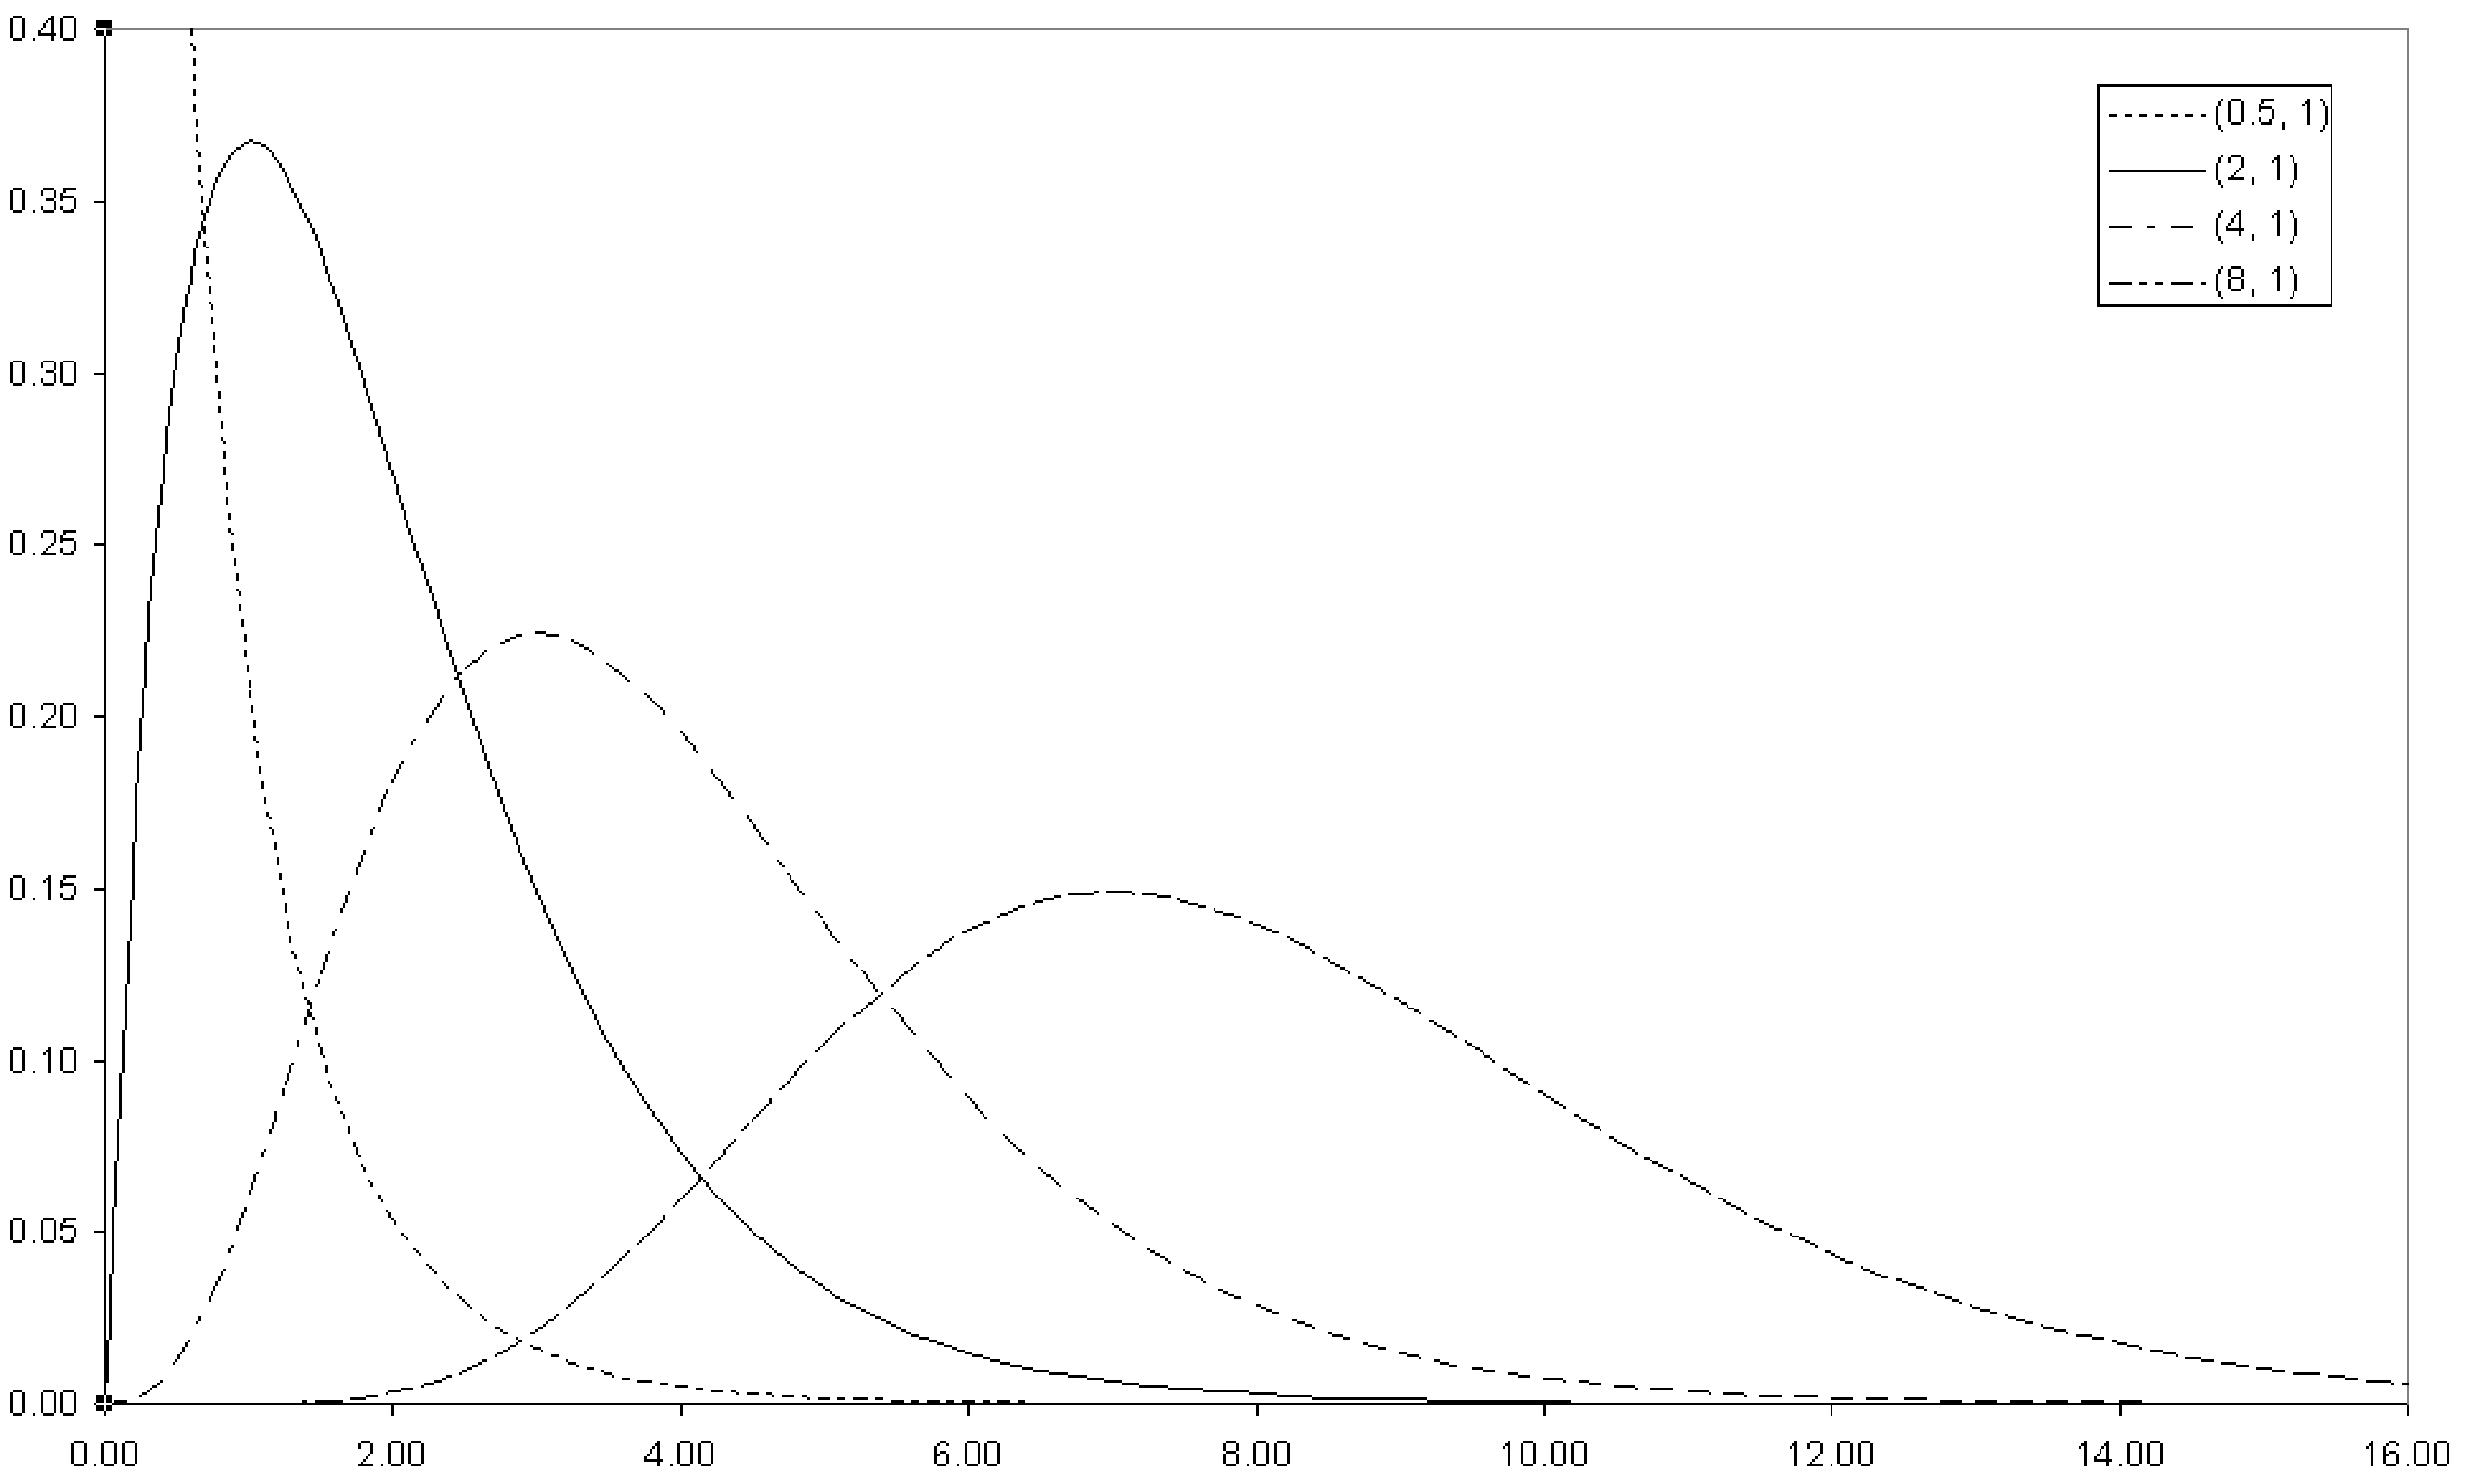
\includegraphics[width=12cm]{Figures/GammaDistribution}
  \caption{Gamma distribution for various values of $\alpha$
  }\label{fig:gammaDistr}
\end{figure}

\subsection{Gamma distribution --- Smalltalk implementation}
\label{sec:sgammadist}\marginpar{Figure
\ref{fig:statisticsclasses} with the box {\textbf GammaDistribution}
grayed.}  Listing \ref{ls:gammadist} shows the implementation of
the gamma distribution in Smalltalk.

The distribution function of the gamma distribution can be
computed with the incomplete gamma function (\cf section
\ref{sec:gammafunc}). Therefore the class {\texttt
DhbGammaDistribution} is implemented as a subclass of {\texttt
DhbProbabilityDensity}.
\begin{listing} Smalltalk implementation of the gamma distribution \label{ls:gammadist}
$$\halign{ #\hfil&\quad#\hfil\cr {\sl Class}& {\Large\bf DhbGammaDistribution}\cr
{\sl Subclass of }&{\tt DhbProbabilityDensity}\cr\noalign{\vskip 1ex}

{\sl Instance variable names:}&\parbox[t]{4 in}{\tt  alpha beta norm randomCoefficients incompleteGammaFunction }\cr\noalign{\vskip 1ex}}$$


Class methods
{\parskip 1ex\par\noindent}
{\bf distributionName}
\begin{verbatim}
    ^ 'Gamma distribution'
\end{verbatim}
{\bf fromHistogram:} {\tt aHistogram}
\begin{verbatim}
    | alpha beta |
    aHistogram minimum < 0
        ifTrue: [ ^nil].
    alpha := aHistogram average.
    beta := aHistogram variance / alpha.
    ^ [ self shape: alpha / beta scale: beta] when: ExAll do: [ 
                                       :signal | signal exitWith: nil]
\end{verbatim}
{\bf new}
\begin{verbatim}
    ^ self error: 'Illegal creation message for this class'
\end{verbatim}
{\bf shape:} {\tt aNumber1} {\bf scale:} {\tt aNumber2}
\begin{verbatim}
    ^ super new initialize: aNumber1 scale: aNumber2
\end{verbatim}

Instance methods
{\parskip 1ex\par\noindent}
{\bf average}
\begin{verbatim}
    ^ alpha * beta
\end{verbatim}
{\bf changeParametersBy:} {\tt aVector}
\begin{verbatim}
    alpha := alpha + ( aVector at: 1).
    beta := beta + ( aVector at: 2).
    self computeNorm.
    incompleteGammaFunction := nil.
    randomCoefficients := nil.
\end{verbatim}
{\bf computeNorm}
\begin{verbatim}
    norm := beta ln * alpha + alpha logGamma.
\end{verbatim}
{\bf distributionValue:} {\tt aNumber}
\begin{verbatim}
    ^ self incompleteGammaFunction value: aNumber / beta
\end{verbatim}
{\bf incompleteGammaFunction}
\begin{verbatim}
    incompleteGammaFunction isNil 
        ifTrue: 
            [ incompleteGammaFunction := DhbIncompleteGammaFunction 
                                                        shape: alpha ].
    ^ incompleteGammaFunction
\end{verbatim}
{\bf initialize:} {\tt aNumber1} {\bf scale:} {\tt aNumber2}
\begin{verbatim}
    (aNumber1 > 0 and: [ aNumber2 > 0])
        ifFalse: [ self error: 'Illegal distribution parameters'].
    alpha := aNumber1.
    beta := aNumber2.
    self computeNorm.
    ^ self
\end{verbatim}
{\bf initializeRandomCoefficientsForLargeAlpha}
\begin{verbatim}
    | a b q d |
    a := 1 / ( 2 * alpha - 1) sqrt.
    b := alpha - (4 ln).
    q := 1 / a + alpha.
    d := 4.5 ln + 1.
    ^ Array with: a with: b with: q with: d
\end{verbatim}
{\bf initializeRandomCoefficientsForSmallAlpha}
\begin{verbatim}
    | e |
    e := 1 exp.
    ^ (e + alpha) / e
\end{verbatim}
{\bf kurtosis}
\begin{verbatim}
    ^ 6 / alpha
\end{verbatim}
{\bf parameters}
\begin{verbatim}
    ^ Array with: alpha with: beta
\end{verbatim}
{\bf random}
\begin{verbatim}
    ^ ( alpha > 1 ifTrue: [ self randomForLargeAlpha]
                        ifFalse:[ self randomForSmallAlpha]) * beta
\end{verbatim}
{\bf randomCoefficientsForLargeAlpha}
\begin{verbatim}
    randomCoefficients isNil
        ifTrue: [ randomCoefficients := self initializeRandomCoefficientsForLargeAlpha].
    ^ randomCoefficients
\end{verbatim}
{\bf randomCoefficientsForSmallAlpha}
\begin{verbatim}
    randomCoefficients isNil
        ifTrue: [ randomCoefficients := self 
                           initializeRandomCoefficientsForSmallAlpha].
    ^ randomCoefficients
\end{verbatim}
{\bf randomForLargeAlpha}
\begin{verbatim}
    [ true] whileTrue: [
    | u1 u2 c v y z w |
    u1 := DhbMitchellMooreGenerator new floatValue.
    u2 := DhbMitchellMooreGenerator new floatValue.
    c := self randomCoefficientsForLargeAlpha.
    v := ( u1 / ( 1 - u1)) ln * (c at: 1).
    y := v exp * alpha.
    z := u1 squared * u2.
    w := ( c at: 3) * v + ( c at: 2) - y.
    ( c at: 4) + w >= ( 4.5 * z) ifTrue: [ ^y].
    z ln <= w ifTrue: [ ^y].
    ].
\end{verbatim}
{\bf randomForSmallAlpha}
\begin{verbatim}
    [ true] whileTrue: [
    | p |
    p := DhbMitchellMooreGenerator new floatValue * self 
                                      randomCoefficientsForSmallAlpha.
    p > 1
        ifTrue: [ | y |
                     y := ( ( self randomCoefficientsForSmallAlpha - 
                                               p) / alpha) ln negated.
                     DhbMitchellMooreGenerator new floatValue <= ( y 
                                               raisedTo: ( alpha - 1))
                        ifTrue: [ ^y].
                    ]
        ifFalse: [ | y |
                        y := p raisedTo: ( 1 / alpha).
                     DhbMitchellMooreGenerator new floatValue <= ( y 
                                                          negated exp)
                        ifTrue: [ ^y].
                     ].
    ].
\end{verbatim}
{\bf skewness}
\begin{verbatim}
    ^ 2 / alpha sqrt
\end{verbatim}
{\bf value:} {\tt aNumber}
\begin{verbatim}
    ^ aNumber > 0
        ifTrue: [ ( aNumber ln * (alpha - 1) - (aNumber / beta) - 
                                                            norm) exp ]
        ifFalse:[ 0 ].
\end{verbatim}
{\bf variance}
\begin{verbatim}
    ^ beta squared * alpha
\end{verbatim}


\end{listing}


\section{Experimental distribution}
A histogram described in section \ref{sec:histogram} can be used
as a probability distribution. After all, a histogram can be
considered as the representation of a distribution, which has been
measured experimentally.

If $N$ is the total count of the histogram and $n_i$ the count in
bin number $i$ the probability of finding a measurement within the
bin number $i$ is simply given by:
\begin{equation}
  P_i={\displaystyle n_i \over\displaystyle N}.
\end{equation}
If $w$ is the width of each bin, the probability density function
of the distribution measured by the histogram can be estimated by:
\begin{equation}
\label{eq:histprob}
  P\left(x\right)={\displaystyle P_i \over\displaystyle w}
  ={\displaystyle n_i \over\displaystyle wN}\mbox{\quad
  where $i=\left\lfloor{\displaystyle x-x_{\min}\over\displaystyle w}\right\rfloor$.}
\end{equation}
Equation \ref{eq:histprob} is only valid for $x_{\min}\le x <
x_{\max}$. Outside of the histogram's limits there is no
information concerning the shape of the probability density
function.

The distribution function is computed by evaluating the sum of all
bins located below the argument and by adding a correction
computed by linear interpolation over the bin in which the value
is located. Thus, we have:
\begin{equation}
\label{eq:histdistr}
  F\left(x\right)={\displaystyle 1 \over\displaystyle N} \left(\sum_{j=1}^{i-1}n_j
  + {x-x_i \over w}n_i\right)
  \mbox{\quad where $i=\left\lfloor{\displaystyle x-x_{\min}\over\displaystyle w}\right\rfloor$.}
\end{equation}
If $x<x_{\min}$, $F\left(x\right)=0$ and if $x\geq x_{\max}$,
$F\left(x\right)=1$. A similar equation can be derived for the
acceptance interval function.

\subsection{Experimental distribution --- General  implementation}
\marginpar{Figure \ref{fig:statisticsclasses} with the box {\textbf
HistogrammedDistribution} grayed.} Adding the responsibility of
behaving like a probability density function to a histogram is not
desirable. In a good object oriented design, objects should have
only one responsibility or type of behavior.

Thus, a good object oriented implementation implements an
\patstyle{Adapter} pattern. One creates an object, having the
behavior of a probability density function. A single instance
variable inside this object refers to the histogram, over which
the experimental distribution is defined. The \patstyle{Adapter}
object is a subclass of the abstract class describing all
probability density functions.

The parameters of the distribution --- average, variance, skewness
and kurtosis --- are obtained from the histogram itself.

The computation of the distribution and the interval acceptance
function is delegated to the histogram. The floor operation of
equation \ref{eq:histdistr} is evaluated by the method {\texttt
binIndex} of the histogram.

\begin{quote}
{\textbf Note:} In both implementation, there is no protection against
illegal arguments. Illegal arguments can occur when computing the
distribution value when the histogram underflow and overflow
counts are non zero. Below the minimum and above the maximum, no
information can be obtained for the distribution. Within the
histogram limits, there is no need for protection. Therefore the
implementation assumes that the histogram was collected using
automatic adjustment of the limits (\cf section
\ref{sec:histogram}).
\end{quote}

\subsection{Experimental distribution --- Smalltalk  implementation}
Listing \ref{ls:histprob} shows the implementation of an
experimental distribution in Smalltalk.

The class {\texttt DhbHistogrammedDistribution} is a subclass of the
class {\texttt DhbProbabilityDensity}. The class creation method {\texttt
histogram:} takes as argument the histogram over which the
instance is defined. To prevent creating a instance with undefined
instance variable, the default class creation method {\texttt new}
returns an error.

\begin{listing} Smalltalk implementation of an experimental distribution \label{ls:histprob}
$$\halign{ #\hfil&\quad#\hfil\cr {\sl Class}& {\Large\bf DhbHistogrammedDistribution}\cr
{\sl Subclass of }&{\tt DhbProbabilityDensity}\cr\noalign{\vskip 1ex}

{\sl Instance variable names:}&\parbox[t]{4 in}{\tt  histogram }\cr\noalign{\vskip 1ex}}$$


Class methods
{\parskip 1ex\par\noindent}
{\bf distributionName}
\begin{verbatim}
    ^ 'Experimental distribution'
\end{verbatim}
{\bf histogram:} {\tt aHistogram}
\begin{verbatim}
    ^ super new initialize: aHistogram
\end{verbatim}
{\bf new}
\begin{verbatim}
    ^ self error: 'Illegal creation message for this class'
\end{verbatim}

Instance methods
{\parskip 1ex\par\noindent}
{\bf acceptanceBetween:} {\tt aNumber1} {\bf and:} {\tt aNumber2}
\begin{verbatim}
    ^ (histogram countsBetween: (aNumber1 max: histogram minimum)
                        and: (aNumber2 min: histogram maximum) ) / 
                                                  histogram totalCount

\end{verbatim}
{\bf average}
\begin{verbatim}
    ^ histogram average

\end{verbatim}
{\bf distributionValue:} {\tt aNumber}
\begin{verbatim}
    ^ aNumber < histogram minimum
        ifTrue: [ 0 ]
        ifFalse:[ aNumber < histogram maximum
                            ifTrue: [ ( histogram countsUpTo: 
                                      aNumber) / histogram totalCount ]
                            ifFalse:[ 1 ]
                    ]
\end{verbatim}
{\bf initialize:} {\tt aHistogram}
\begin{verbatim}
    aHistogram count = 0
        ifTrue: [ self error: 'Cannot define probability density on 
                                                 an empty histogram'].
    histogram := aHistogram.
    ^ self
\end{verbatim}
{\bf kurtosis}
\begin{verbatim}
    ^ histogram kurtosis
\end{verbatim}
{\bf privateInverseDistributionValue:} {\tt aNumber}
\begin{verbatim}
    ^ histogram inverseDistributionValue: aNumber
\end{verbatim}
{\bf skewness}
\begin{verbatim}
    ^ histogram skewness
\end{verbatim}
{\bf standardDeviation}
\begin{verbatim}
    ^ histogram standardDeviation
\end{verbatim}
{\bf value:} {\tt aNumber}
\begin{verbatim}
    ^ (aNumber >= histogram minimum and: [ aNumber < histogram 
                                                             maximum])
        ifTrue: [ ( histogram countAt: aNumber) / ( histogram 
                                     totalCount * histogram binWidth)]
        ifFalse:[ 0 ]
\end{verbatim}
{\bf variance}
\begin{verbatim}
    ^ histogram variance
\end{verbatim}


\end{listing}


%\ifx\wholebook\relax\else\end{document}\fi

%%\ifx\wholebook\relax\else
%\documentclass[twoside]{book}
%\usepackage[active]{srcltx}
%\usepackage[LY1]{fontenc}
%\usepackage{url}
\makeatletter
\def\url@leostyle{%
  \@ifundefined{selectfont}{\def\UrlFont{\sf}}{\def\UrlFont{\sffamily}}}
\makeatother
% Now actually use the newly defined style.
\urlstyle{leo}

\usepackage{graphicx}
\def\etc{{\textit{etc}}}
\def\eg{{\textit{e.g.}}}
\def\ie{{\textit{i.e.}}}
\def\cf{{\textit{c.f.}}\ }
\def\erf{\mathop{\textrm{erf}}}
\def\sign{\mathop{\textrm{sign}}}
\def\prob{\mathop{\textrm{Prob}}}
\def\var{\mathop{\textrm{var}}}
\def\mod{\mathop{\textrm{mod}}}
\def\cor{\mathop{\textrm{cor}}}
\def\cov{\mathop{\textrm{cov}}}
\def\cl{\mathop{\textrm{CL}}}
\def\kg{\mathop{\textrm{Kg}}}
\def\patstyle#1{{\textsc #1}}
\def\th{^{\mathop{\textrm{th}}}}
%\def\st#1{^{\mathop{\rm #1}}}
\def\note#1{\begin{quote}{\textbf{Note:}} #1\end{quote}}
\def\braket#1{\left\langle #1\right\rangle}
\def\order#1{\let\o=#1$\mathcal{O}$\ifx\o 1$\left(n\right)$\else$\left(n^{#1}\right)$\fi}
%\newtheorem{privListing}{Listing}[chapter]
%\newenvironment{listing}{\vskip 3ex\hrule\vskip 1ex\begin{privListing}}{\end{privListing}\hrule\vskip 1ex}
\newtheorem{privExample}{Code example}[chapter]
\newenvironment{codeExample}{\begin{privExample}\begin{quote}\tt}{\end{quote}\end{privExample}}
\def\relboxl#1#2{\hbox to #1\hsize{#2\hfil}}
\def\relboxc#1#2{\hbox to #1\hsize{\hfil #2\hfil}}
\def\relboxr#1#2{\hbox to #1\hsize{\hfil #2}}
\def\transpose#1{\textbf{#1}^{\mathop\textrm{T}}}
\def\inverse#1{\textbf{#1}^{-1}}
%\def\tm{$^{\mathop{\rm TM}}$}
\def\tm{ }
\newenvironment{mainEquation}{\marginpar[\vspace{3 ex} Main
equation$\Rightarrow$]{\vspace{3 ex}$\Leftarrow$Main
equation}\begin{equation}}{\end{equation}}
\def\rubrique#1{\paragraph{#1}\hfil\par\noindent}

%\begin{document}
%\fi

\chapter{Statistical analysis}
\label{ch:estimation}
\begin{flushright}
{\textsl L'expérience instruit plus sûrement que le
conseil.}\footnote{Experience teaches more surely than
counseling.}\\ André Gide
\end{flushright}
\vspace{1 ex}This chapter is dedicated on how to extract
information from large amount of data using statistical analysis.
One of the best book I have read on this subject is titled {\textsl
How to lies with statistics}\footnote{D. Huff, {\textsl How to lies
  with statistics}, Norton and Co., New York 1954.}.
This admittedly slanted title seems a little pessimistic.
The truth, however, is that most people in their daily job ignore the little statistics
they have learned in high school.
As a result, statistical argumentation is often used wrongly to produce the wrong
conclusions.

The problems addressed in this section pertain to the
interpretation of experimental measurements.
For a long time such a discipline was reserved to physicists only. Recently natural
science disciplines discovered that statistics could be used
effectively to verify hypotheses or to determine parameters based
on experimental observations.
Today, the best papers on statistics and estimations are found primarily in natural science
publications (Biometrika \eg).
Recently, the use of statistics has been extended to financial analysis.

Statistics can be applied to experimental data in two ways.
Firstly, one can test the consistency and/or accuracy of the data.
These tests are the subject of the first 3 sections. Secondly, the
values of unknown parameters can be derived from experimental
data. This very important aspect of statistical analysis is
treated in the remaining of the chapter.

Figure \ref{fig:estimationclasses} shows the classes described in
this chapter.
\begin{figure}
\centering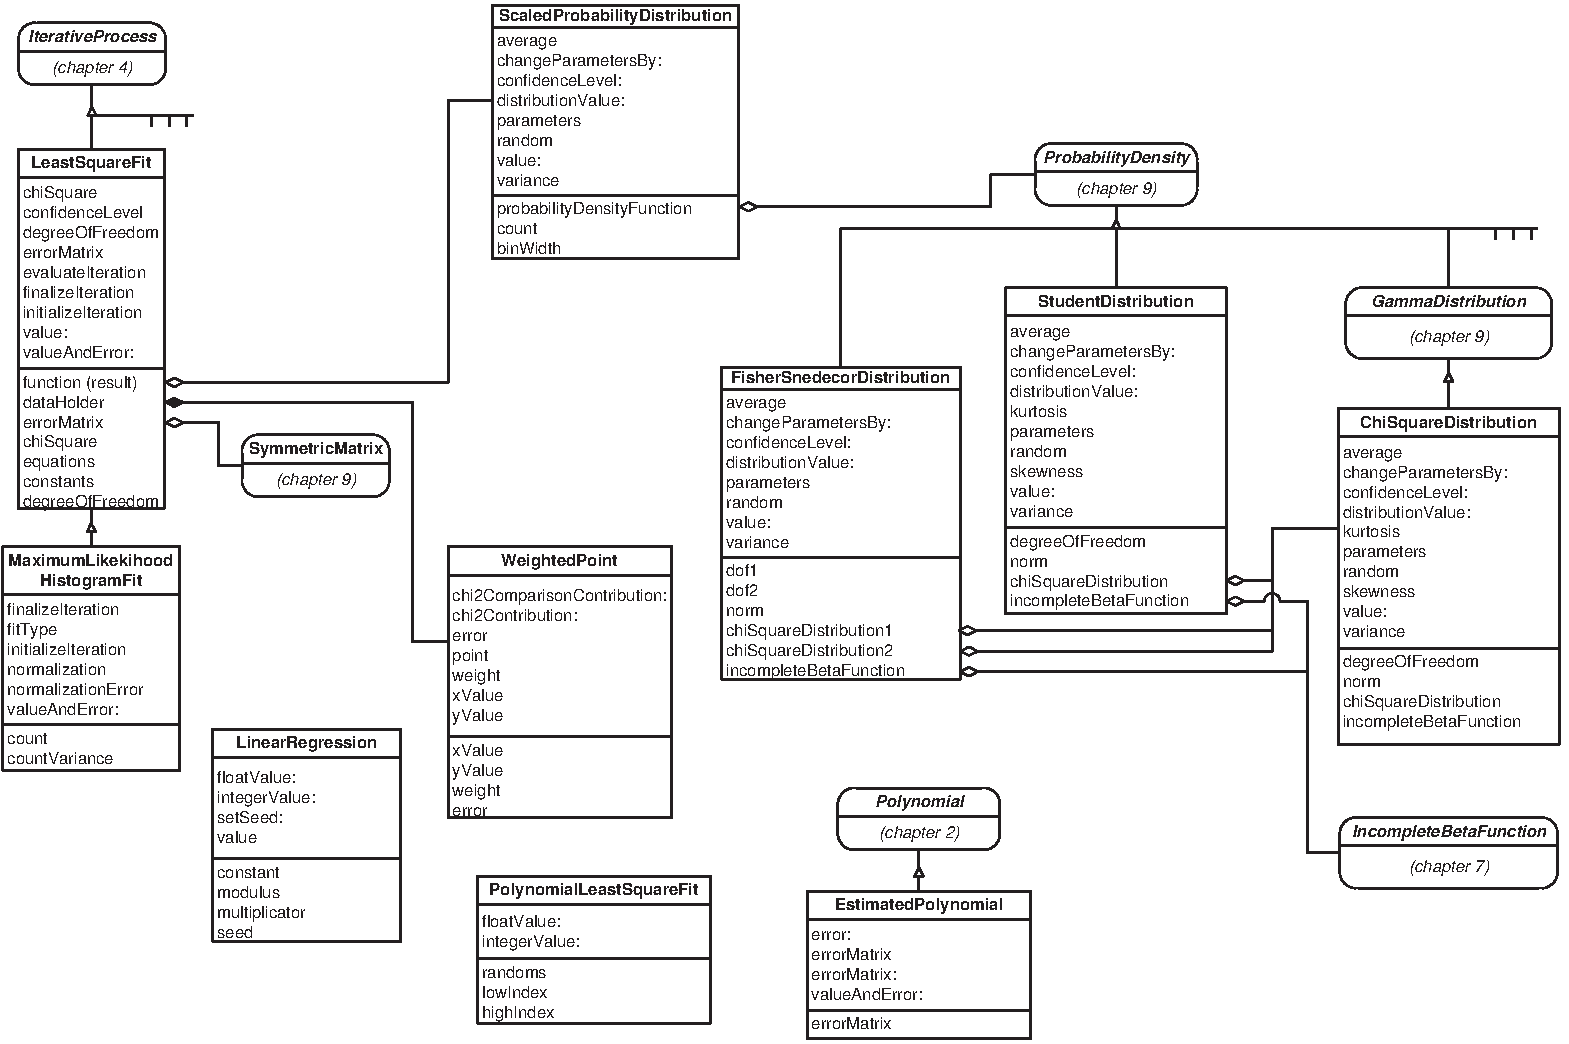
\includegraphics[width=11cm]{Figures/EstimationClasses}
\caption{Classes related to estimation}
\label{fig:estimationclasses}
\end{figure}
The reader should be aware that the techniques used for non-linear
least square fits (section \ref{sec:lsfnonlin}) can also be also
applied to solve systems of non-linear equations.

\section{$F$-test and the Fisher-Snedecor distribution}
\label{sec:Ftest} The $F$-test tries to answer the following
question: given two series of measurements, $x_1,\ldots,x_n$ and
$y_1,\ldots,y_m$, what is the probability that the two
measurements have the same standard deviation? The $F$-test is
used when there are not enough statistics to perform a detailed
analysis of the data.

Let us assume that the distribution of the two random variables,
$x$ and $y$, are normal distributions with respective averages
$\mu_x$ and $\mu_y$, and respective standard deviations $\sigma_x$
and $\sigma_y$. Then, $\bar{s}_x$, the standard deviation of
$x_1,\ldots,x_n$ is an estimator of $\sigma_x$; $\bar{s}_y$, the
standard deviation of $y_1,\ldots,y_m$ is an estimator of
$\sigma_y$. The following statistics
\begin{equation}
  F={\displaystyle \bar{s}_x^2\over\sigma_x^2}\cdot{\displaystyle\sigma_y^2\over\bar{s}_y^2}
\end{equation}
can be shown to be distributed according to a Fisher-Snedecor
distribution with degrees of freedom $n$ and $m$. In particular,
if one wants to test for the equality of the two standard
deviations, one construct the following statistics:
\begin{equation}
\label{eq:Ftest}
  F={\displaystyle \bar{s}_x^2\over\bar{s}_y^2}.
\end{equation}
Traditionally one chooses $\bar{s}_x>\bar{s}_y$ so that the
variable $F$ is always greater than one.

It is important to recall that the expression above is distributed
according to a Fisher-Snedecor distribution if and only if the two
sets of data are distributed according to a normal distribution.
For experimental measurements this is often the case unless
systematic errors are present. Nevertheless this assumption must
be verified before making an $F$-test.

Table \ref{tb:Fdist} shows the properties of the Fisher-Snedecor
distribution. The Fisher-Snedecor distribution is itself rarely
used as a probability density function, however.
\begin{table}[h]
  \centering
  \caption{Properties of the Fisher-Snedecor distribution}\label{tb:Fdist}
\vspace{1 ex}
\begin{tabular}{|l|c|} \hline
  \vbox to 3ex{}Range of random variable & $\left[0,+\infty\right[$\\ *[1ex] \hline
  \vbox to 5ex{}Probability density function & $\displaystyle P\left(x\right)=
  {n_1^{n_1\over 2}n_2^{n_2\over 2}x^{n_1-1\over 2}
  \over B\left({n_1\over 2},{n_2\over 2}\right)
  \left(n_1+n_2 x\right)^{n_1+n_2\over 2}
  }$ \\*[3ex]  \hline
  \vbox to 3ex{}Parameters & $n_1,n_2$ \\
  & two positive integers\\*[1ex]  \hline
  \vbox to 5ex{}Distribution function & $\displaystyle F\left(x\right)=
  B\left({n_1\over n_1+n_2x};{n_1\over 2},{n_2\over 2}\right)$ \\*[1ex]  \hline
  \vbox to 4ex{}Average & $\displaystyle{n_2\over n_2-2}$\quad for $n>2$ \\*[2ex]
  & undefined otherwise\\*[1ex] \hline
  \vbox to 5ex{}Variance & $\displaystyle{2n_2^2\left(n_1+n_2-2\right)\over
  n_1\left(n_2-2\right)^2\left(n_2-4\right)}$\quad for $n>4$ \\*[3ex]
  & undefined otherwise\\*[1ex] \hline
  \vbox to 3ex{}Skewness & $ $ \\*[1ex] \hline
  \vbox to 3ex{}Kurtosis & $ $ \\*[1ex] \hline
\end{tabular}
\end{table}

The main part of figure \ref{fig:fsnedecorDistr} shows the shape
of the Fisher-Snedecor distribution for some values of the degrees
of freedom.
\begin{figure}
\centering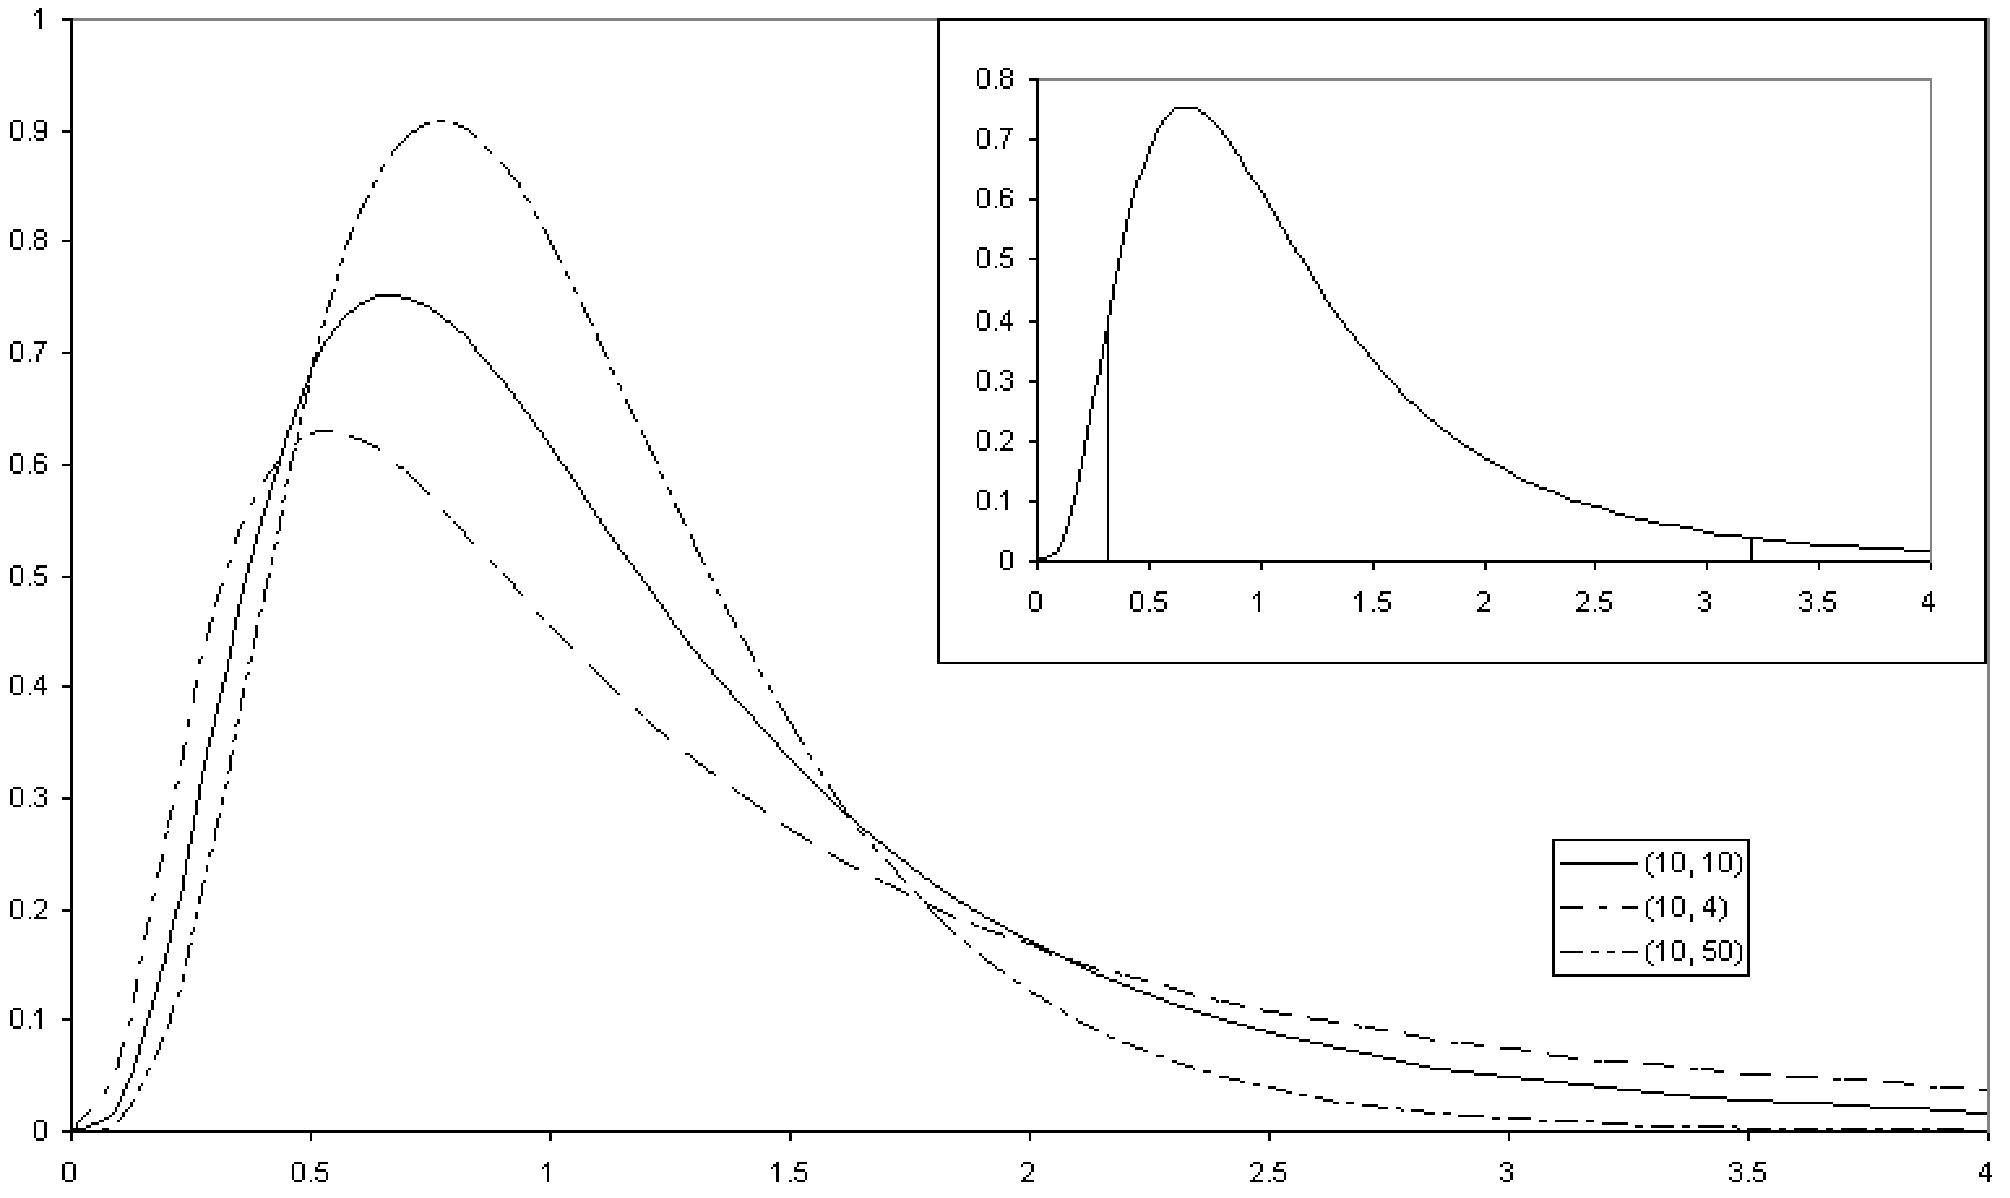
\includegraphics[width=12cm]{Figures/FisherSnedecorDistribution}
\caption{Fisher-Snedecor distribution for a few parameters}\label{fig:fsnedecorDistr}
\end{figure}
For large $n$ and $m$, the Fisher-Snedecor distribution
tends toward a normal distribution.


The confidence level of a Fisher-Snedecor distribution is defined
as the probability expressed in percent of finding a value larger
than $F$ defined in equation \ref{eq:Ftest} or lower than $1/F$.
The confidence level is thus related to the distribution function.
We have:
\begin{equation}
\label{eq:fcl}
  {\cl}_F\left(x,n\right)=100\left\{1-\left[F\left(x\right)-F\left({1\over x}\right)
  \right]\right\},
\end{equation}
where $x$ is the value $F$ defined in equation \ref{eq:Ftest}. The
change of notation was made to avoid confusion between the
acceptance function and the random variable.  The confidence level
corresponds to the surface of the shaded areas in the insert in
the upper right corner of figure \ref{fig:fsnedecorDistr}.

\rubrique{Example.} Here is an example used to investigate the
goodness of the two random number generators discussed in section
\ref{sec:random}. The collected data are the error of the
covariance test described in section \ref{sec:random}. The
dimension of the covariance matrix is 7 and the number of trials
on each measurement was 1000. The table \ref{tb:Ftest} presents
the obtained results, expressed in ${1\over 1000}$.
\begin{table}[h]
\vspace{1 ex}
  \centering
  \caption{Covariance test of random number generator}\label{tb:Ftest}
\vspace{1 ex}
  \begin{tabular}{|c|c|c|} \hline
     & Congruential & Mitchell-Moore \\ \hline
    1 & 5.56 & 7.48 \\
    2 & 5.89 & 6.75 \\
    3 & 4.66 & 3.77 \\
    4 & 5.69 & 5.71 \\
    5 & 5.34 & 7.25 \\
    6 & 4.79 & 4.73 \\
    7 & 4.80 & 6.23 \\
    8 & 7.86 & 5.60 \\
    9 & 3.64 & 5.94 \\
    10 & 5.70 & 4.58 \\ \hline
    Average & 5.40 & 5.80 \\
    Std. dev. & 1.10 & 1.19 \\ \hline
  \end{tabular}
\end{table}
the ratio of the two variances is $1.18$ and the degrees of
freedom are both 10. The F-test applied to the two variances gives
a confidence level of $20\%$. This means that there is only a
$20\%$ probability that the variances of the two series of
measurements are different.

\subsection{Fisher-Snedecor distribution --- Smalltalk implementation}
\marginpar{Figure \ref{fig:estimationclasses} with the box {\textbf
FisherSnedecorDistribution} grayed.} Listing \ref{ls:Fdist} shows
the implementation of the Fisher-Snedecor distribution in
Smalltalk. Listing \ref{ls:Ftest} shows the implementation of the
$F$-test in Smalltalk. The following code example shows how to
perform a $F$-test between two sets of experimental measurements.

\label{exs:Ftest}
\begin{displaycode}{Smalltalk}
 | mom1 mom2 confidenceLevel |
 mom1 := PMFixedStatisticalMoments new.
\end{displaycode}

\hfil{\texttt<\textsl Collecting measurements of set 1 into \texttt
mom1>}\hfil
\begin{displaycode}{Smalltalk}
 mom2 := PMFixedStatisticalMoments new.
\end{displaycode}
\hfil{\texttt<\textsl Collecting measurements of set 2 into \texttt
mom1>}\hfil
\begin{displaycode}{Smalltalk}
 confidenceLevel := mom1 fConfidenceLevel: mom2.
\end{displaycode}

Two instances of statistical moments (\cf section
\ref{sec:srobustmoment}) are created. Experimental data are
accumulated into each set separately (\cf code example
\ref{ex:smoments}). The last line returns the probability in
percent that the two sets of data have the same standard
deviation.

The class {\texttt PMFisherSnedecorDistribution} is implemented as a
subclass of {\texttt PMProbabilityDensity} because its distribution
function can be computed numerically using the incomplete beta
function (\cf section \ref{sec:incbeta}).

\begin{listing}[label=ls:Fdist]{Smalltalk}
{Smalltalk implementation of the Fisher-Snedecor distribution}
PMProbabilityDensity subclass: #PMFisherSnedecorDistribution
  instanceVariableNames: 'dof1 dof2 norm chiSquareDistribution1
  chiSquareDistribution2 incompleteBetaFunction'
  classVariableNames: ''
  package: 'Math-DistributionForHistogram'
\end{listing}

\begin{displaycode}{Smalltalk}
PMFisherSnedecorDistribution class >> degreeOfFreedom: anInteger1
degreeOfFreedom: anInteger2
    ^ super new initialize: anInteger1 and: anInteger2
\end{displaycode}

\begin{displaycode}{Smalltalk}
PMFisherSnedecorDistribution class >> distributionName
    ^ 'Fisher-Snedecor distribution'
\end{displaycode}

\begin{displaycode}{Smalltalk}
PMFisherSnedecorDistribution class >> fromHistogram: aHistogram
    | n1 n2 a |
    aHistogram minimum < 0 ifTrue: [^nil].
    n2 := (2 / (1 - (1 / aHistogram average))) rounded.
    n2 > 0 ifFalse: [^nil].
    a := (n2 - 2) * (n2 - 4) * aHistogram variance / (n2 squared * 
                                                                   2).
    n1 := (0.7 * (n2 - 2) / (1 - a)) rounded.
    ^n1 > 0 
        ifTrue: [self degreeOfFreedom: n1 degreeOfFreedom: n2]
        ifFalse: [nil]
\end{displaycode}

\begin{displaycode}{Smalltalk}
PMFisherSnedecorDistribution class >> new
 ^ self error: 'Illegal creation message for this class'
\end{displaycode} 

\begin{displaycode}{Smalltalk}
PMFisherSnedecorDistribution class >> test: aStatisticalMoment1 with: aStatisticalMoment2
    ^ (self class degreeOfFreedom: aStatisticalMoment1 count
        degreeOfFreedom: aStatisticalMoment2 count) 
            distributionValue: aStatisticalMoment1 variance 
                    / aStatisticalMoment2 variance
\end{displaycode}

\begin{displaycode}{Smalltalk}
PMFisherSnedecorDistribution >> average
    ^dof2 > 2
        ifTrue: [ dof2 / ( dof2 - 2) ]
        ifFalse:[ nil ]
\end{displaycode}
      
\begin{displaycode}{Smalltalk}
PMFisherSnedecorDistribution >> changeParametersBy: aVector
    dof1 := (dof1 + (aVector at: 1)) max: 1.
    dof2 := (dof2 + (aVector at: 2)) max: 1.
    self computeNorm.
    chiSquareDistribution1 := nil.
    chiSquareDistribution2 := nil.
    incompleteBetaFunction := nil
\end{displaycode}
  
\begin{displaycode}{Smalltalk}
PMFisherSnedecorDistribution >> computeNorm
    norm := (dof1 ln * (dof1 / 2)) + (dof2 ln * (dof2 / 2))
                        - ((dof1 / 2) logBeta: (dof2 / 2))
\end{displaycode}

\begin{displaycode}{Smalltalk}
PMFisherSnedecorDistribution >> confidenceLevel: aNumber
    aNumber < 0
        ifTrue: [ self error: 'Confidence level argument must be 
                                                           positive'].
    ^((self distributionValue: aNumber) - ( self distributionValue: 
                                           aNumber reciprocal) ) * 100
\end{displaycode}

\begin{displaycode}{Smalltalk}
PMFisherSnedecorDistribution >> distributionValue: aNumber
    ^ 1 - ( self incompleteBetaFunction value: ( dof2 / ( aNumber * 
                                                        dof1 + dof2)))
\end{displaycode}

\begin{displaycode}{Smalltalk}
PMFisherSnedecorDistribution >> incompleteBetaFunction
    incompleteBetaFunction isNil 
        ifTrue: 
            [incompleteBetaFunction := PMIncompleteBetaFunction 
                                                       shape: dof2 / 2
                        shape: dof1 / 2].
    ^incompleteBetaFunction
\end{displaycode}

\begin{displaycode}{Smalltalk}
PMFisherSnedecorDistribution >> initialize: anInteger1 and: anInteger2
    dof1 := anInteger1.
    dof2 := anInteger2.
    self computeNorm.
    ^ self
\end{displaycode}

\begin{displaycode}{Smalltalk}
PMFisherSnedecorDistribution >> parameters
    ^ Array with: dof1 with: dof2
\end{displaycode}

\begin{displaycode}{Smalltalk}
PMFisherSnedecorDistribution >> random
    chiSquareDistribution1 isNil
        ifTrue: [ chiSquareDistribution1 := PMChiSquareDistribution 
                                                degreeOfFreedom: dof1.
                  chiSquareDistribution2 := PMChiSquareDistribution 
                                                degreeOfFreedom: dof2.
                ].
    ^chiSquareDistribution1 random * dof2 / ( chiSquareDistribution2 
                                                        random * dof1)
\end{displaycode}

\begin{displaycode}{Smalltalk}
PMFisherSnedecorDistribution >> value: aNumber
    ^aNumber > 0
        ifTrue: [ (norm + ( aNumber ln * (dof1 / 2 - 1)) - ( 
             (aNumber * dof1 + dof2) ln * (( dof1 + dof2) / 2))) exp]
        ifFalse:[ 0 ]
\end{displaycode}

\begin{displaycode}{Smalltalk}
PMFisherSnedecorDistribution >> variance
    ^ dof2 > 4 ifTrue: [ dof2 squared * 2 * ( dof1 + dof2 - 2) / ( ( 
                              dof2 - 2) squared * dof1 * ( dof2 - 4))]
                   ifFalse:[ nil ]
\end{displaycode}

The computation of the confidence level for the $F$-test is
implemented in the method {\texttt fConfidenceLevel:} of the class
{\texttt PMStatisticalMoments}. It calculates the statistics $F$
according to equation \ref{eq:Ftest}, creates an instance of a
Fisher-Snedecor distribution and passes the value of $F$ to the
method {\texttt confidenceLevel:} of the distribution. The method {\texttt
fConfidenceLevel:} is also implemented by the class {\texttt
Histogram} where it is simply delegated to the statistical moments
accumulated by the histogram. The argument of the method can be a
statistical moment or a histogram since the messages sent by the
method are polymorphic to both classes.

\begin{listing} Smalltalk implementation of the $F$-test \label{ls:Ftest}
$$\halign{ #\hfil&\quad#\hfil\cr {\sl Class}& {\Large\bf DhbStatisticalMoments}\cr
{\sl Subclass of }&{\tt Object}\cr\noalign{\vskip 1ex}

{\sl Instance variable names:}&\parbox[t]{4 in}{\tt  moments }\cr\noalign{\vskip 1ex}}$$


Instance methods
{\parskip 1ex\par\noindent}
{\bf fConfidenceLevel:} {\tt aStatisticalMomentsOrHistogram}
\begin{verbatim}
    | fValue |
    fValue := self variance/ aStatisticalMomentsOrHistogram variance.
    ^ fValue < 1
        ifTrue: [ (DhbFisherSnedecorDistribution degreeOfFreedom: 
                                  aStatisticalMomentsOrHistogram count
                        degreeOfFreedom: self count) 
                                        confidenceLevel: fValue 
                                                           reciprocal ]
        ifFalse: [ (DhbFisherSnedecorDistribution degreeOfFreedom: 
                                                            self count
                        degreeOfFreedom: 
                                aStatisticalMomentsOrHistogram count) 
                                        confidenceLevel: fValue ]
\end{verbatim}


$$\halign{ #\hfil&\quad#\hfil\cr {\sl Class}& {\Large\bf DhbHistogram}\cr
{\sl Subclass of }&{\tt Object}\cr\noalign{\vskip 1ex}

{\sl Instance variable names:}&\parbox[t]{4 in}{\tt  minimum binWidth overflow underflow moments contents freeExtent cacheSize desiredNumberOfBins }\cr\noalign{\vskip 1ex}}$$

Instance methods
{\parskip 1ex\par\noindent}
{\bf fConfidenceLevel:} {\tt aStatisticalMomentsOrHistogram}
\begin{verbatim}
    ^ moments fConfidenceLevel: aStatisticalMomentsOrHistogram
\end{verbatim}


\end{listing}

\section{$t$-test and the Student distribution}
\label{sec:ttest} The $t$-test tries to answer the following
question: given two series of measurements, $x_1,\ldots,x_n$ and
$y_1,\ldots,y_m$, what is the probability that the two
measurements have the same average?  The $t$-test is used when
there are not enough statistics to perform a detailed analysis of
the data.

Let us assume that the distribution of the two random variables,
$x$ and $y$, are normal distributions with respective averages
$\mu_x$ and $\mu_y$, and the same standard deviation $\sigma$.
Then $\bar{x}$, the average of $x_1,\ldots,x_n$ is an estimator of
$\mu_x$; $\bar{y}$, the average of $y_1,\ldots,y_m$ is an
estimator of $\mu_y$. An estimation $\bar{s}$ of the standard
deviation $\sigma$ can be made using both measurement samples. We
have:
\begin{equation}
\label{eq:sbart}
  \bar{s}^2={\displaystyle\sum_{i=1}^n\left(x_i-\bar{x}\right)^2
  + \sum_{i=1}^m\left(y_i-\bar{y}\right)^2\over\displaystyle n+m-2}.
\end{equation}
One can prove that the following statistics:
\begin{equation}
  t={\displaystyle \left(\bar{x}-\bar{y}\right)-\left(\mu_x
  -\mu_y\right)
  \over\displaystyle \bar{s}\sqrt{{1\over n}+{1\over m}}}
\end{equation}
is distributed according to a Student distribution with $n+m-2$
degrees of freedom. In particular, to test for the probability
that the two series of measurements have the same average, one
uses the following statistics:
\begin{equation}
\label{eq:tTest}
  t={\displaystyle \bar{x}-\bar{y}
  \over\displaystyle \bar{s}\sqrt{{1\over n}+{1\over m}}}.
\end{equation}
It is important to recall the two fundamental hypotheses that have
been made so far.
\begin{enumerate}
  \item The two sets of data must be distributed according to a normal distribution.
  \item The two sets of data must have the same standard deviation.
\end{enumerate}
Too many people use the $t$-test without first checking the
assumptions. Assumption 1 is usually fulfilled with experimental
measurements in the absence of systematic errors. Assumption 2.
however, must be checked, for example using the F-test discussed
in section \ref{sec:Ftest}.

Because the random variable of the distribution is traditionally
labeled $t$, this distribution is often called the
$t$-distribution. Table \ref{tb:tdist} shows the properties of the
Student distribution. The Student distribution is itself rarely
used as a probability density function, however.
\begin{table}[h]
  \centering
  \caption{Properties of the Student distribution}\label{tb:tdist}
\vspace{1 ex}
\begin{tabular}{|l|c|} \hline
  \vbox to 3ex{}Range of random variable & $\left]-\infty,+\infty\right[$\\ *[1ex] \hline
  \vbox to 5ex{}Probability density function & $\displaystyle P\left(x\right)=
  {1\over\sqrt{n}B\left({n\over 2},{1\over 2}\right)}
  \left(1+{t^2\over n}\right)^{-{n+1\over 2}}$ \\*[2ex]  \hline
  \vbox to 3ex{}Parameters & $n$ \\
  & a positive integer\\*[1ex]  \hline
  \vbox to 4ex{}Distribution function &
  \parbox{6cm}{$$F\left(x\right)=\left\{
  \begin{array}{ll}
  {1 + B\left({n\over n + x^2};{n\over 2},{1\over 2}\right)\over 2}&\mbox{\quad for
  $x\ge 0$}\\*[1ex]
  {1 - B\left({n\over n + x^2};{n\over 2},{1\over 2}\right)\over 2}&\mbox{\quad for $x<0$}
  \end{array}\right.$$} \\*[1ex]  \hline
  \vbox to 3ex{}Average & $0$ \\*[1ex] \hline
  \vbox to 3ex{}Variance & ${n\over n-2}$\quad for $n>2$\\
  & undefined otherwise\\*[1ex] \hline
  \vbox to 3ex{}Skewness & $0$ \\*[1ex] \hline
  \vbox to 3ex{}Kurtosis & ${6\over n-4}$\quad for $n>4$\\
  & undefined otherwise\\*[1ex] \hline
\end{tabular}
\end{table}

For $n=1$, the Student distribution is identical to a Cauchy
distribution with $\mu=0$ and $\beta=1$. For large $n$, the
Student distribution tends toward a normal distribution with
average 0 and variance 1. The main part of figure
\ref{fig:studentDistr} shows the shapes of the Student
distribution for a few values of the degrees of freedom. The
normal distribution is also given for comparison.
\begin{figure}
\centering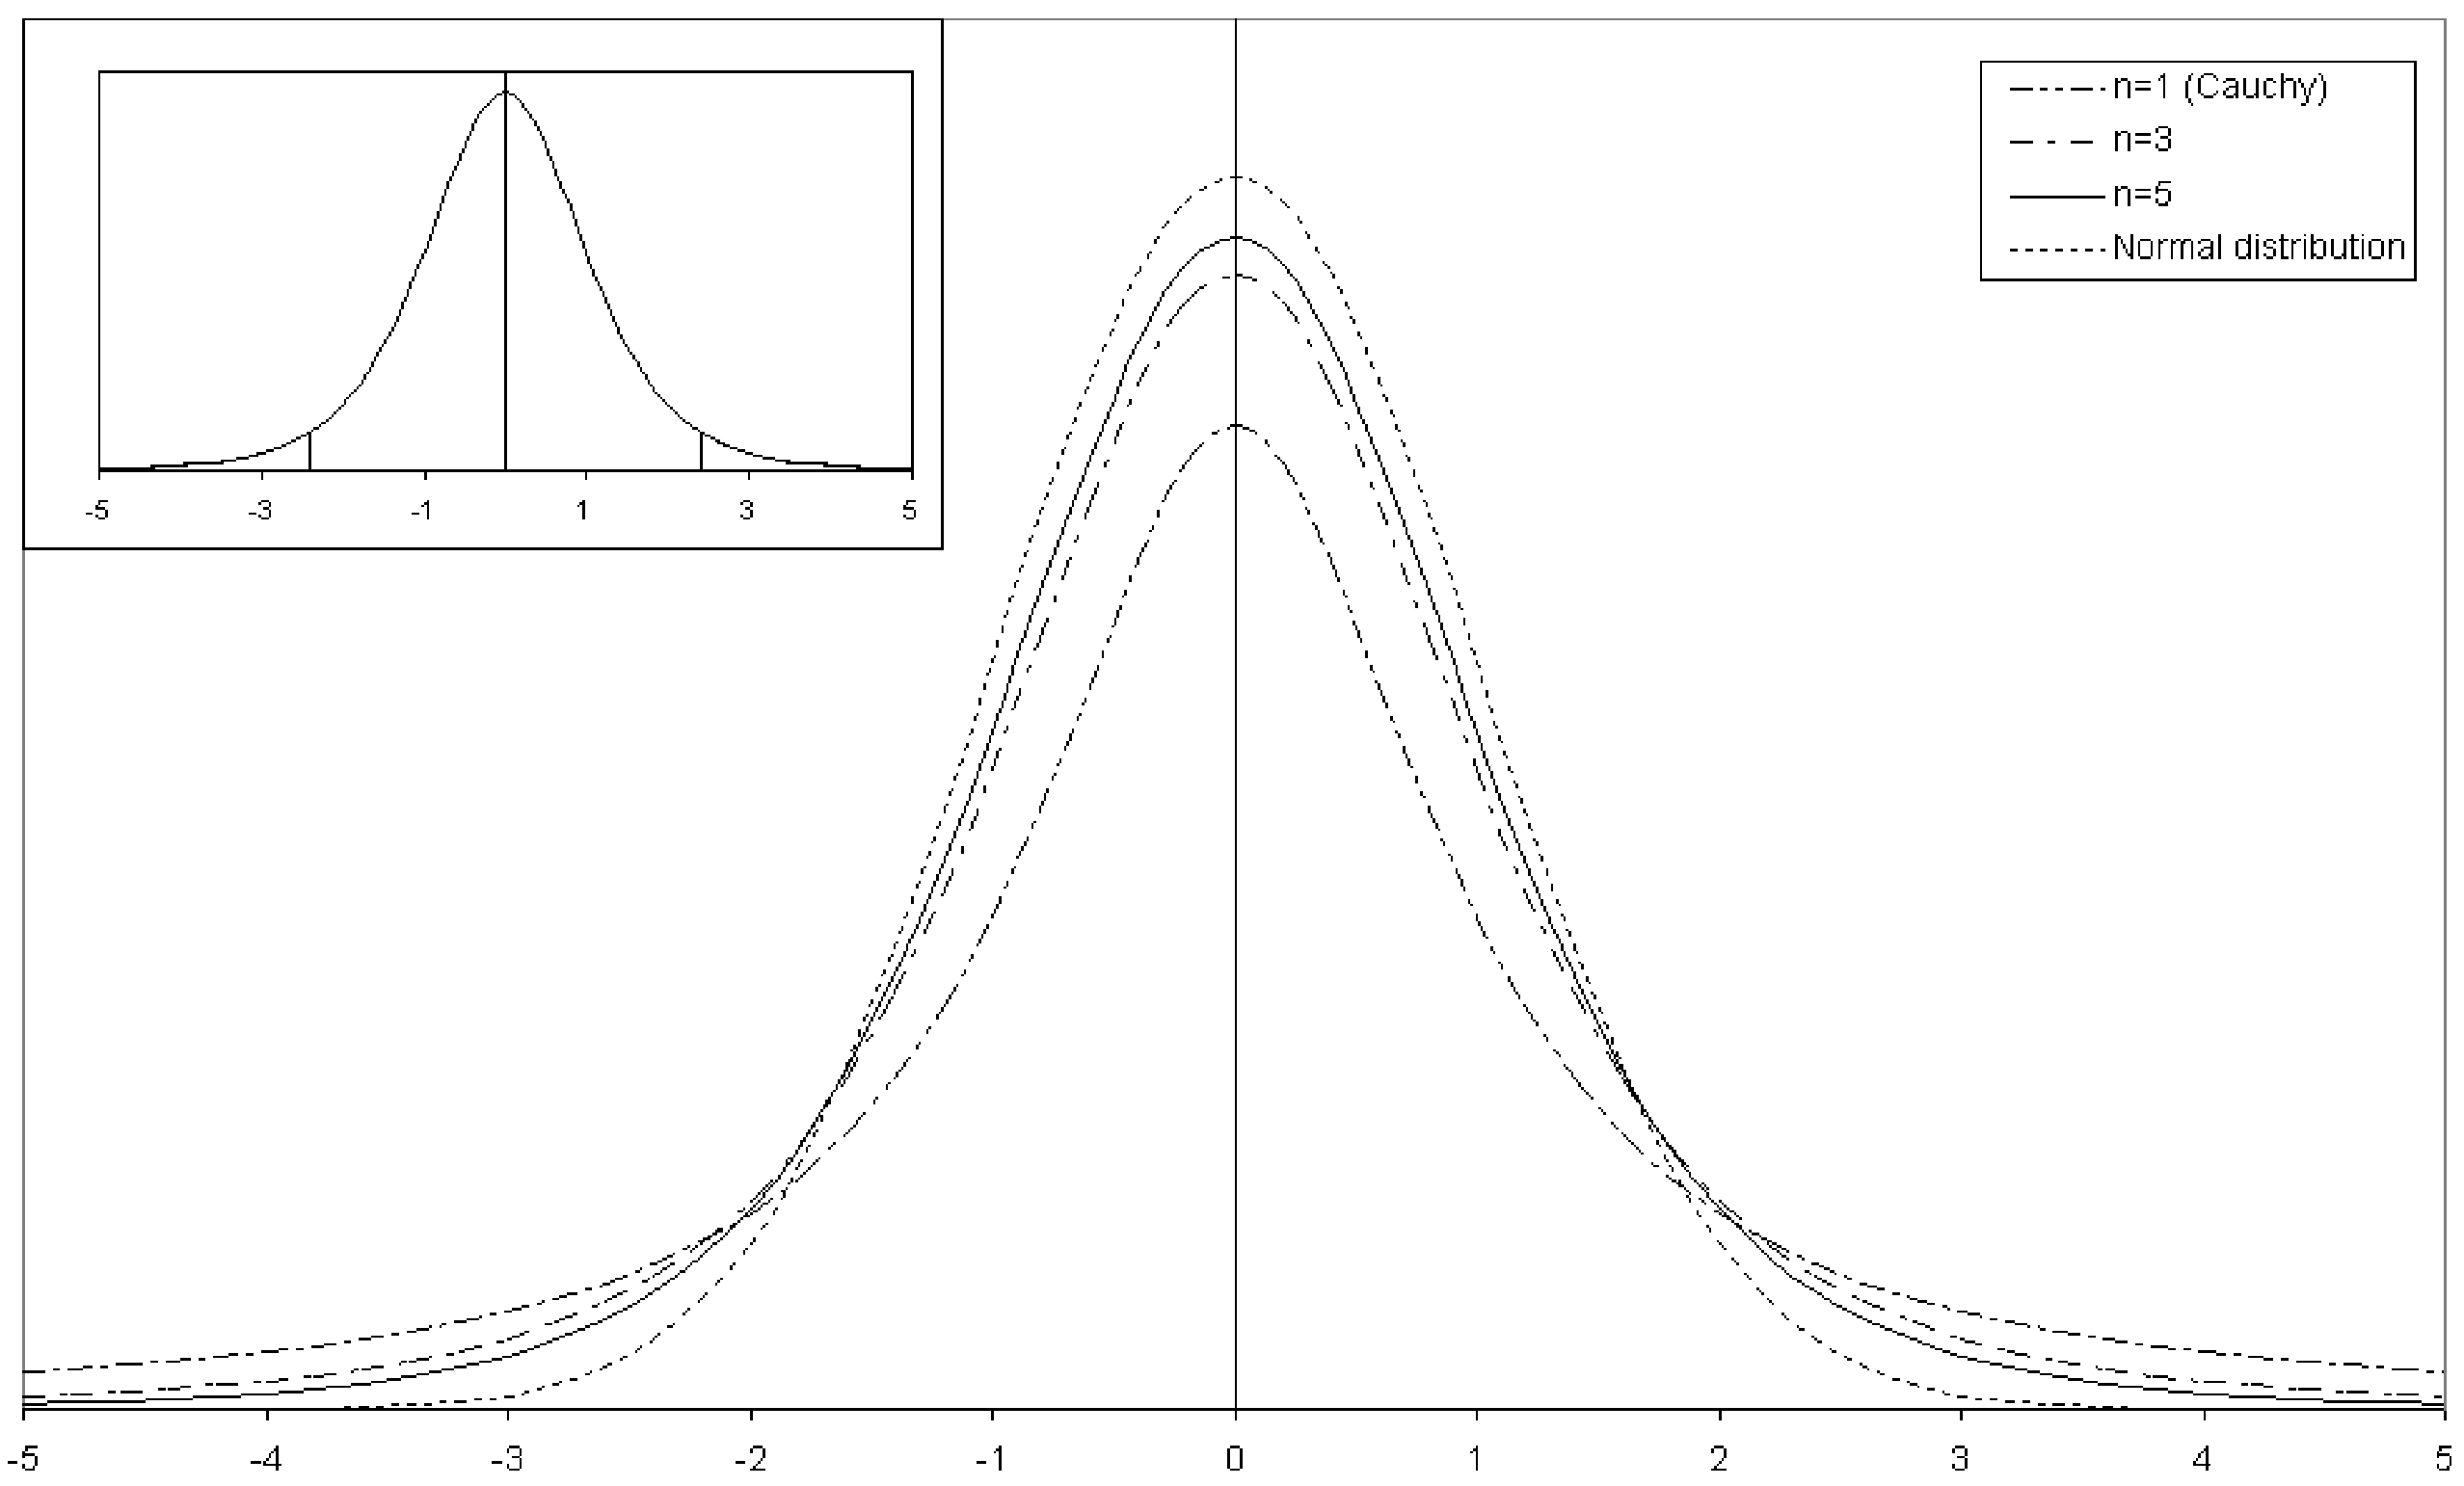
\includegraphics[width=12cm]{Figures/StudentDistribution}
\caption{Student distribution for a few degrees of freedom
}\label{fig:studentDistr}
\end{figure}


The confidence level of a Student distribution is defined as the
probability to find a value whose absolute value is larger than a
given value. Thus, it estimates the level of confidence that the
hypothesis --- namely, that the two sets of measurements have the
same average --- cannot be accepted. Traditionally the confidence
level is given in percent. The confidence level corresponds to the
surface of shaded area in the insert in the upper left corner of
figure \ref{fig:studentDistr}. By definition, the confidence level
is related to the interval acceptance function:
\begin{equation}
\label{eq:tcl}
  {\cl}_t\left(t,n\right)=100\left[1-
  F\left(-\left|t\right|,\left|t\right|\right)\right],
\end{equation}
using the definition of the interval acceptance function (equation
\ref{eq:defacceptdiff}). The value of $t$ in equation \ref{eq:tcl}
is obtained from equation \ref{eq:tTest}.

The distribution function of the Student distribution is
calculated with the incomplete beta function (\cf section
\ref{sec:incbeta}). Using the fact that the distribution is
symmetric, one can derive the following expression
\begin{equation}
\label{eq:tsymacc}
  F\left(-\left|t\right|,\left|t\right|\right)=B\left({n\over n + t^2};{n\over 2},{1\over
  2}\right),
\end{equation}
from the properties of the distribution (\cf table \ref{tb:tdist})
and using equations \ref{eq:tcl} and \ref{eq:incBetaFunction}.

\rubrique{Example} Now, we shall continue the analysis of the
results of table \ref{tb:Ftest}. The $t$ value computed from the
two sets of measurements is $0.112$ for a degree of freedom of 18.
the corresponding confidence level is $8.76\%$. That is, there is
only a $8.76\%$ probability that the two generators have a
different behavior. Thus, we can conclude that the Mitchell-Moore
random generator is as good as the congruential random generator.

\subsection{Student distribution --- Smalltalk implementation}
\marginpar{Figure \ref{fig:estimationclasses} with the box {\textbf
StudentDistribution} grayed.} Listing \ref{ls:tdist} shows the
implementation of the Student distribution in Smalltalk. Listing
\ref{ls:tTest} shows the implementation of the $t$-test in
Smalltalk. Performing a $t$-test between two sets of experimental
measurements is very similar to performing a $F$-test. In code
example \ref{exs:Ftest} it suffices to replace the last line with
the following:
\begin{displaycode}
 confidenceLevel := mom1 fConfidenceLevel: mom2.
\end{displaycode}
This last line returns the probability in percent that the two
sets of data have the same average provided that the two sets have
the same standard deviation.

The class {\texttt PMStudentDistribution} is implemented as a
subclass of {\texttt PMProbabilityDensity} because its distribution
function can be computed numerically using the incomplete beta
function (\cf section \ref{sec:incbeta}).

The method {\texttt symmetricAcceptance:} computes the symmetric
acceptance function defined by equation \ref{eq:tsymacc}. This
method is used to compute the disribution function and the
confidence level. The method {\texttt confidenceLevel:} gives the
confidence level in percent.
\begin{listing} Smalltalk implementation of the Student distribution \label{ls:tdist}
$$\halign{ #\hfil&\quad#\hfil\cr {\sl Class}& {\Large\bf DhbStudentDistribution}\cr
{\sl Subclass of }&{\tt DhbProbabilityDensity}\cr\noalign{\vskip 1ex}

{\sl Instance variable names:}&\parbox[t]{4 in}{\tt  degreeOfFreedom norm chiSquareDistribution incompleteBetaFunction }\cr\noalign{\vskip 1ex}}$$


Class methods
{\parskip 1ex\par\noindent}
{\bf asymptoticLimit}
\begin{verbatim}
    ^ 30
\end{verbatim}
{\bf degreeOfFreedom:} {\tt anInteger}
\begin{verbatim}
    ^anInteger > self asymptoticLimit 
        ifTrue: [DhbNormalDistribution new]
        ifFalse: 
            [anInteger = 1 
                ifTrue: [DhbCauchyDistribution shape: 0 scale: 1]
                ifFalse: [super new initialize: anInteger]]
\end{verbatim}
{\bf distributionName}
\begin{verbatim}
    ^'Student distribution'
\end{verbatim}
{\bf fromHistogram:} {\tt aHistogram}
\begin{verbatim}
    | dof var |
    var := aHistogram variance.
    var = 0
        ifTrue: [ ^nil].
    dof :=  ( 2 / (1 - (1 / aHistogram variance))) rounded max: 1.
    ^dof > self asymptoticLimit ifTrue: [ nil]
                                ifFalse:[ self degreeOfFreedom: dof]
\end{verbatim}
{\bf new}
\begin{verbatim}
    ^self error: 'Illegal creation message for this class'
\end{verbatim}
{\bf test:} {\tt aStatisticalMoment1} {\bf with:} {\tt aStatisticalMoment2}
\begin{verbatim}
    | t |
    t := ( aStatisticalMoment1 average - aStatisticalMoment2 average) 
                                                                  abs.
    ^1 - ( ( self class degreeOfFreedom: (  aStatisticalMoment1 count 
  + aStatisticalMoment2 count - 2)) acceptanceBetween: t negated and: 
  t)
\end{verbatim}



Instance methods
{\parskip 1ex\par\noindent}
{\bf average}
\begin{verbatim}
    ^ 0
\end{verbatim}
{\bf changeParametersBy:} {\tt aVector}
\begin{verbatim}
    degreeOfFreedom := degreeOfFreedom + ( aVector at: 1).
    self computeNorm.
\end{verbatim}
{\bf chiSquareDistribution}
\begin{verbatim}
    chiSquareDistribution isNil
        ifTrue: [ chiSquareDistribution := DhbChiSquareDistribution 
                              degreeOfFreedom: (degreeOfFreedom - 1)].
    ^ chiSquareDistribution
\end{verbatim}
{\bf computeNorm}
\begin{verbatim}
    norm := ( ( degreeOfFreedom / 2 logBeta: ( 1 / 2) ) + ( 
                                     degreeOfFreedom ln / 2)) negated.
\end{verbatim}
{\bf confidenceLevel:} {\tt aNumber}
\begin{verbatim}
    ^ (1 - (self symmetricAcceptance: aNumber abs)) * 100
\end{verbatim}
{\bf distributionValue:} {\tt aNumber}
\begin{verbatim}
    aNumber = 0
        ifTrue: [ ^0.5].
    ^ (aNumber > 0
        ifTrue: [ 2 - (self symmetricAcceptance: aNumber abs) ]
        ifFalse:[ self symmetricAcceptance: aNumber abs ]) / 2

\end{verbatim}
{\bf incompleteBetaFunction}
\begin{verbatim}
    incompleteBetaFunction isNil 
        ifTrue: 
            [incompleteBetaFunction := DhbIncompleteBetaFunction 
                        shape: degreeOfFreedom / 2
                        shape: 0.5].
    ^ incompleteBetaFunction
\end{verbatim}
{\bf initialize:} {\tt anInteger}
\begin{verbatim}
    anInteger > 0
        ifFalse: [ self error: 'Degree of freedom must be positive'].
    degreeOfFreedom := anInteger.
    self computeNorm.
    ^ self
\end{verbatim}
{\bf kurtosis}
\begin{verbatim}
    ^ degreeOfFreedom > 4 ifTrue: [ 6 / ( degreeOfFreedom - 4)]
                         ifFalse: [ nil ]
\end{verbatim}
{\bf parameters}
\begin{verbatim}
    ^Array with: degreeOfFreedom
\end{verbatim}
{\bf random}
\begin{verbatim}
    ^DhbNormalDistribution random * ( ( (degreeOfFreedom - 1) / self 
                                  chiSquareDistribution random ) sqrt)
\end{verbatim}
{\bf skewness}
\begin{verbatim}
    ^ 0
\end{verbatim}
{\bf symmetricAcceptance:} {\tt aNumber}
\begin{verbatim}
    ^ self incompleteBetaFunction value: ( degreeOfFreedom / ( 
                                   aNumber squared + degreeOfFreedom))
\end{verbatim}
{\bf value:} {\tt aNumber}
\begin{verbatim}
    ^(norm - ((aNumber squared / degreeOfFreedom + 1) ln * ( ( 
                                       degreeOfFreedom + 1) / 2))) exp
\end{verbatim}
{\bf variance}
\begin{verbatim}
    ^ degreeOfFreedom > 2 ifTrue: [ degreeOfFreedom / ( 
                                                 degreeOfFreedom - 2) ]
                         ifFalse:[ nil ]
\end{verbatim}


\end{listing}

The computation of the confidence level for the $t$-test is
implemented in the method {\texttt tConfidenceLevel:} of the class
{\texttt PMStatisticalMoments}. It calculates the statistics $t$
according to equation \ref{eq:tTest}, creates an instance of a
Student distribution and passes the value of $t$ to the method
{\texttt confidenceLevel:} of the distribution. The method {\texttt
tConfidenceLevel:} is also implemented by the class {\texttt
Histogram} where it is simply delegated to the statistical moments
accumulated by the histogram. The argument of the method can be a
statistical moment or a histogram since the messages sent by the
method are polymorphic to both classes.

The method {\texttt unnormalizedVariance} of class {\texttt
PMStatisticalMoments} corresponds to each sums in the numerator
of equation \ref{eq:sbart}. To allow performing a $t$-test also
with instances of class {\texttt PMFastStatisticalMoments}, it was
necessary to define this for that class.

\begin{listing} Smalltalk implementation of the $t$-test \label{ls:tTest}
$$\halign{ #\hfil&\quad#\hfil\cr {\sl Class}& {\Large\bf DhbStatisticalMoments}\cr
{\sl Subclass of }&{\tt Object}\cr\noalign{\vskip 1ex}

{\sl Instance variable names:}&\parbox[t]{4 in}{\tt  moments }\cr\noalign{\vskip 1ex}}$$


Instance methods
{\parskip 1ex\par\noindent}
{\bf tConfidenceLevel:} {\tt aStatisticalMomentsOrHistogram}
\begin{verbatim}
    | sbar dof |
    dof := self count + aStatisticalMomentsOrHistogram count - 2.
    sbar := ( ( self unnormalizedVariance + 
     aStatisticalMomentsOrHistogram unnormalizedVariance) / dof) sqrt.
    ^( DhbStudentDistribution degreeOfFreedom: dof)
        confidenceLevel: ( self average - 
                             (aStatisticalMomentsOrHistogram average))
                            / ( ( 1 / self count + ( 
                   aStatisticalMomentsOrHistogram count)) sqrt * sbar)

\end{verbatim}


$$\halign{ #\hfil&\quad#\hfil\cr {\sl Class}& {\Large\bf DhbFastStatisticalMoments}\cr
{\sl Subclass of }&{\tt DhbStatisticalMoments}\cr\noalign{\vskip 1ex}
}$$


Instance methods
{\parskip 1ex\par\noindent}
{\bf unnormalizedVariance}
\begin{verbatim}
    ^ (moments at: 3) - ((moments at: 2) squared * self count)
\end{verbatim}


$$\halign{ #\hfil&\quad#\hfil\cr {\sl Class}& {\Large\bf DhbHistogram}\cr
{\sl Subclass of }&{\tt Object}\cr\noalign{\vskip 1ex}

{\sl Instance variable names:}&\parbox[t]{4 in}{\tt  minimum binWidth overflow underflow moments contents freeExtent cacheSize desiredNumberOfBins }\cr\noalign{\vskip 1ex}}$$


Instance methods
{\parskip 1ex\par\noindent}
{\bf tConfidenceLevel:} {\tt aStatisticalMomentsOrHistogram}
\begin{verbatim}
    ^moments tConfidenceLevel: aStatisticalMomentsOrHistogram

\end{verbatim}
{\bf unnormalizedVariance}
\begin{verbatim}
    ^moments unnormalizedVariance

\end{verbatim}


\end{listing}

\section{$\chi^2$-test and $\chi^2$ distribution}
\label{sec:chitest} The $\chi^2$-test tries to answer the
following question: how well a theory is able to predict observed
results? Alternatively a $\chi^2$-test can also tell whether two
independent sets of observed results are compatible. This latter
formulation is less frequently used than the former. Admittedly
these two questions are somewhat vague. We shall now put them in
mathematical terms for a more precise definition.

Let us assume that the measurement of an observable quantity
depends on some parameters. These parameters cannot be adjusted by
the experimenter but can be measured exactly\footnote{Of course,
there is no such thing as an exact measurement. The measurement of
the parameters must be far more precise than that of the observed
quantity.}. Let $x_p$ be the measured values of the observed
quantity where $p$ is a label for the parameters; let $\sigma_p$
be the standard deviation of $x_p$.

The first question assumes that one can predict the values of the
observed quantity: let $\mu_p$ be the predicted value of $x_p$.
Then the quantity:
\begin{equation}
  y_p = { x_p - \mu_p \over \sigma_p}
\end{equation}
is distributed according to a normal distribution with average 0
and standard deviation 1 if and only if the quantities $x_p$ are
distributed according to a normal distribution with average
$\mu_p$ and standard deviation $\sigma_p$.

A $\chi^2$ distribution with $n$ degrees of freedom describes the
distribution of the sum of the squares of $n$ random variables
distributed according to a normal distribution with mean 0 and
standard deviation 1. Thus, the following quantity
\begin{equation}
\label{eq:defchitest}
  S=\sum_p { \left(x_p - \mu_p\right)^2\over \sigma_p^2}
\end{equation}
is distributed according to a $\chi^2$ distribution with $n$
degrees of freedom where $n$ is the number of available
measurements (that is the number of terms in the sum of equation
\ref{eq:defchitest}).

To formulate the second question one must introduce a second set
of measurement of the same quantity and at the same values of the
parameters. Let $x^{\prime}_p$ be the second set of measured
values and $\sigma^{\prime}_p$ the corresponding standard
deviations. The estimated standard deviation for the difference
$x_p - x^{\prime}_p$ is $\sqrt{\sigma_p^2+\sigma^{\prime 2}_p }$.
If the two sets of measurements are compatible, the quantity
\begin{equation}
  y^{\prime}_p = { x_p - x^{\prime}_p \over
  \sqrt{\sigma_p^2+\sigma^{\prime 2}_p}}
\end{equation}
is distributed according to a normal distribution with average 0
and standard deviation 1. Then the following quantity
\begin{equation}
\label{eq:defchitestcmp}
  S=\sum_p { \left(x_p - x^{\prime}_p\right)^2\over \sigma_p^2+\sigma^{\prime 2}_p2}
\end{equation}
is distributed according to a $\chi^2$ distribution with $n$
degrees of freedom.

Table \ref{tb:chi2dist} shows the properties of the $\chi^2$
distribution.
\begin{table}[h]
  \centering
  \caption{Properties of the $\chi^2$ distribution}\label{tb:chi2dist}
\vspace{1 ex}
\begin{tabular}{|l|c|} \hline
  \vbox to 3ex{}Range of random variable & $\left[0,+\infty\right[$\\ *[1ex] \hline
  \vbox to 5ex{}Probability density function & $\displaystyle P\left(x\right)=
  {\displaystyle x^{{n\over 2}-1}e^{-{x\over 2}}
  \over\displaystyle 2^{n\over 2}\Gamma\left({n\over 2}\right)}$ \\*[4ex]  \hline
  \vbox to 3ex{}Parameters & $n$ \\
  & a positive integer\\*[1ex]  \hline
  \vbox to 4ex{}Distribution function & $\displaystyle F\left(x\right)=
  \Gamma\left({x\over 2};{n\over 2}\right)$ \\*[1ex]  \hline
  \vbox to 3ex{}Average & $n$ \\*[1ex] \hline
  \vbox to 3ex{}Variance & $2n$ \\*[1ex] \hline
  \vbox to 4ex{}Skewness & $2\sqrt{\displaystyle 2\over\displaystyle n}$ \\*[1ex] \hline
  \vbox to 4ex{}Kurtosis & ${\displaystyle 12\over\displaystyle n}$ \\*[1ex] \hline
\end{tabular}
\end{table}
It is a special case of the gamma distribution with
$\alpha={n\over 2}$ and $\beta=2$ (\cf section
\ref{sec:gammadist}). For $n>30$ one can prove that the variable
$y=\sqrt{2x}-\sqrt{2n-1}$ is approximately distributed according
to a normal distribution with average 0 and standard deviation 1.
If $n$ is very large the $\chi^2$ distribution tends toward a
normal distribution with average $n$ and standard deviation
$\sqrt{2n}$.

Figure \ref{fig:chi2Distr} shows the shape of the $\chi^2$
distribution for a few values of the degree of freedom.
\begin{figure}
\centering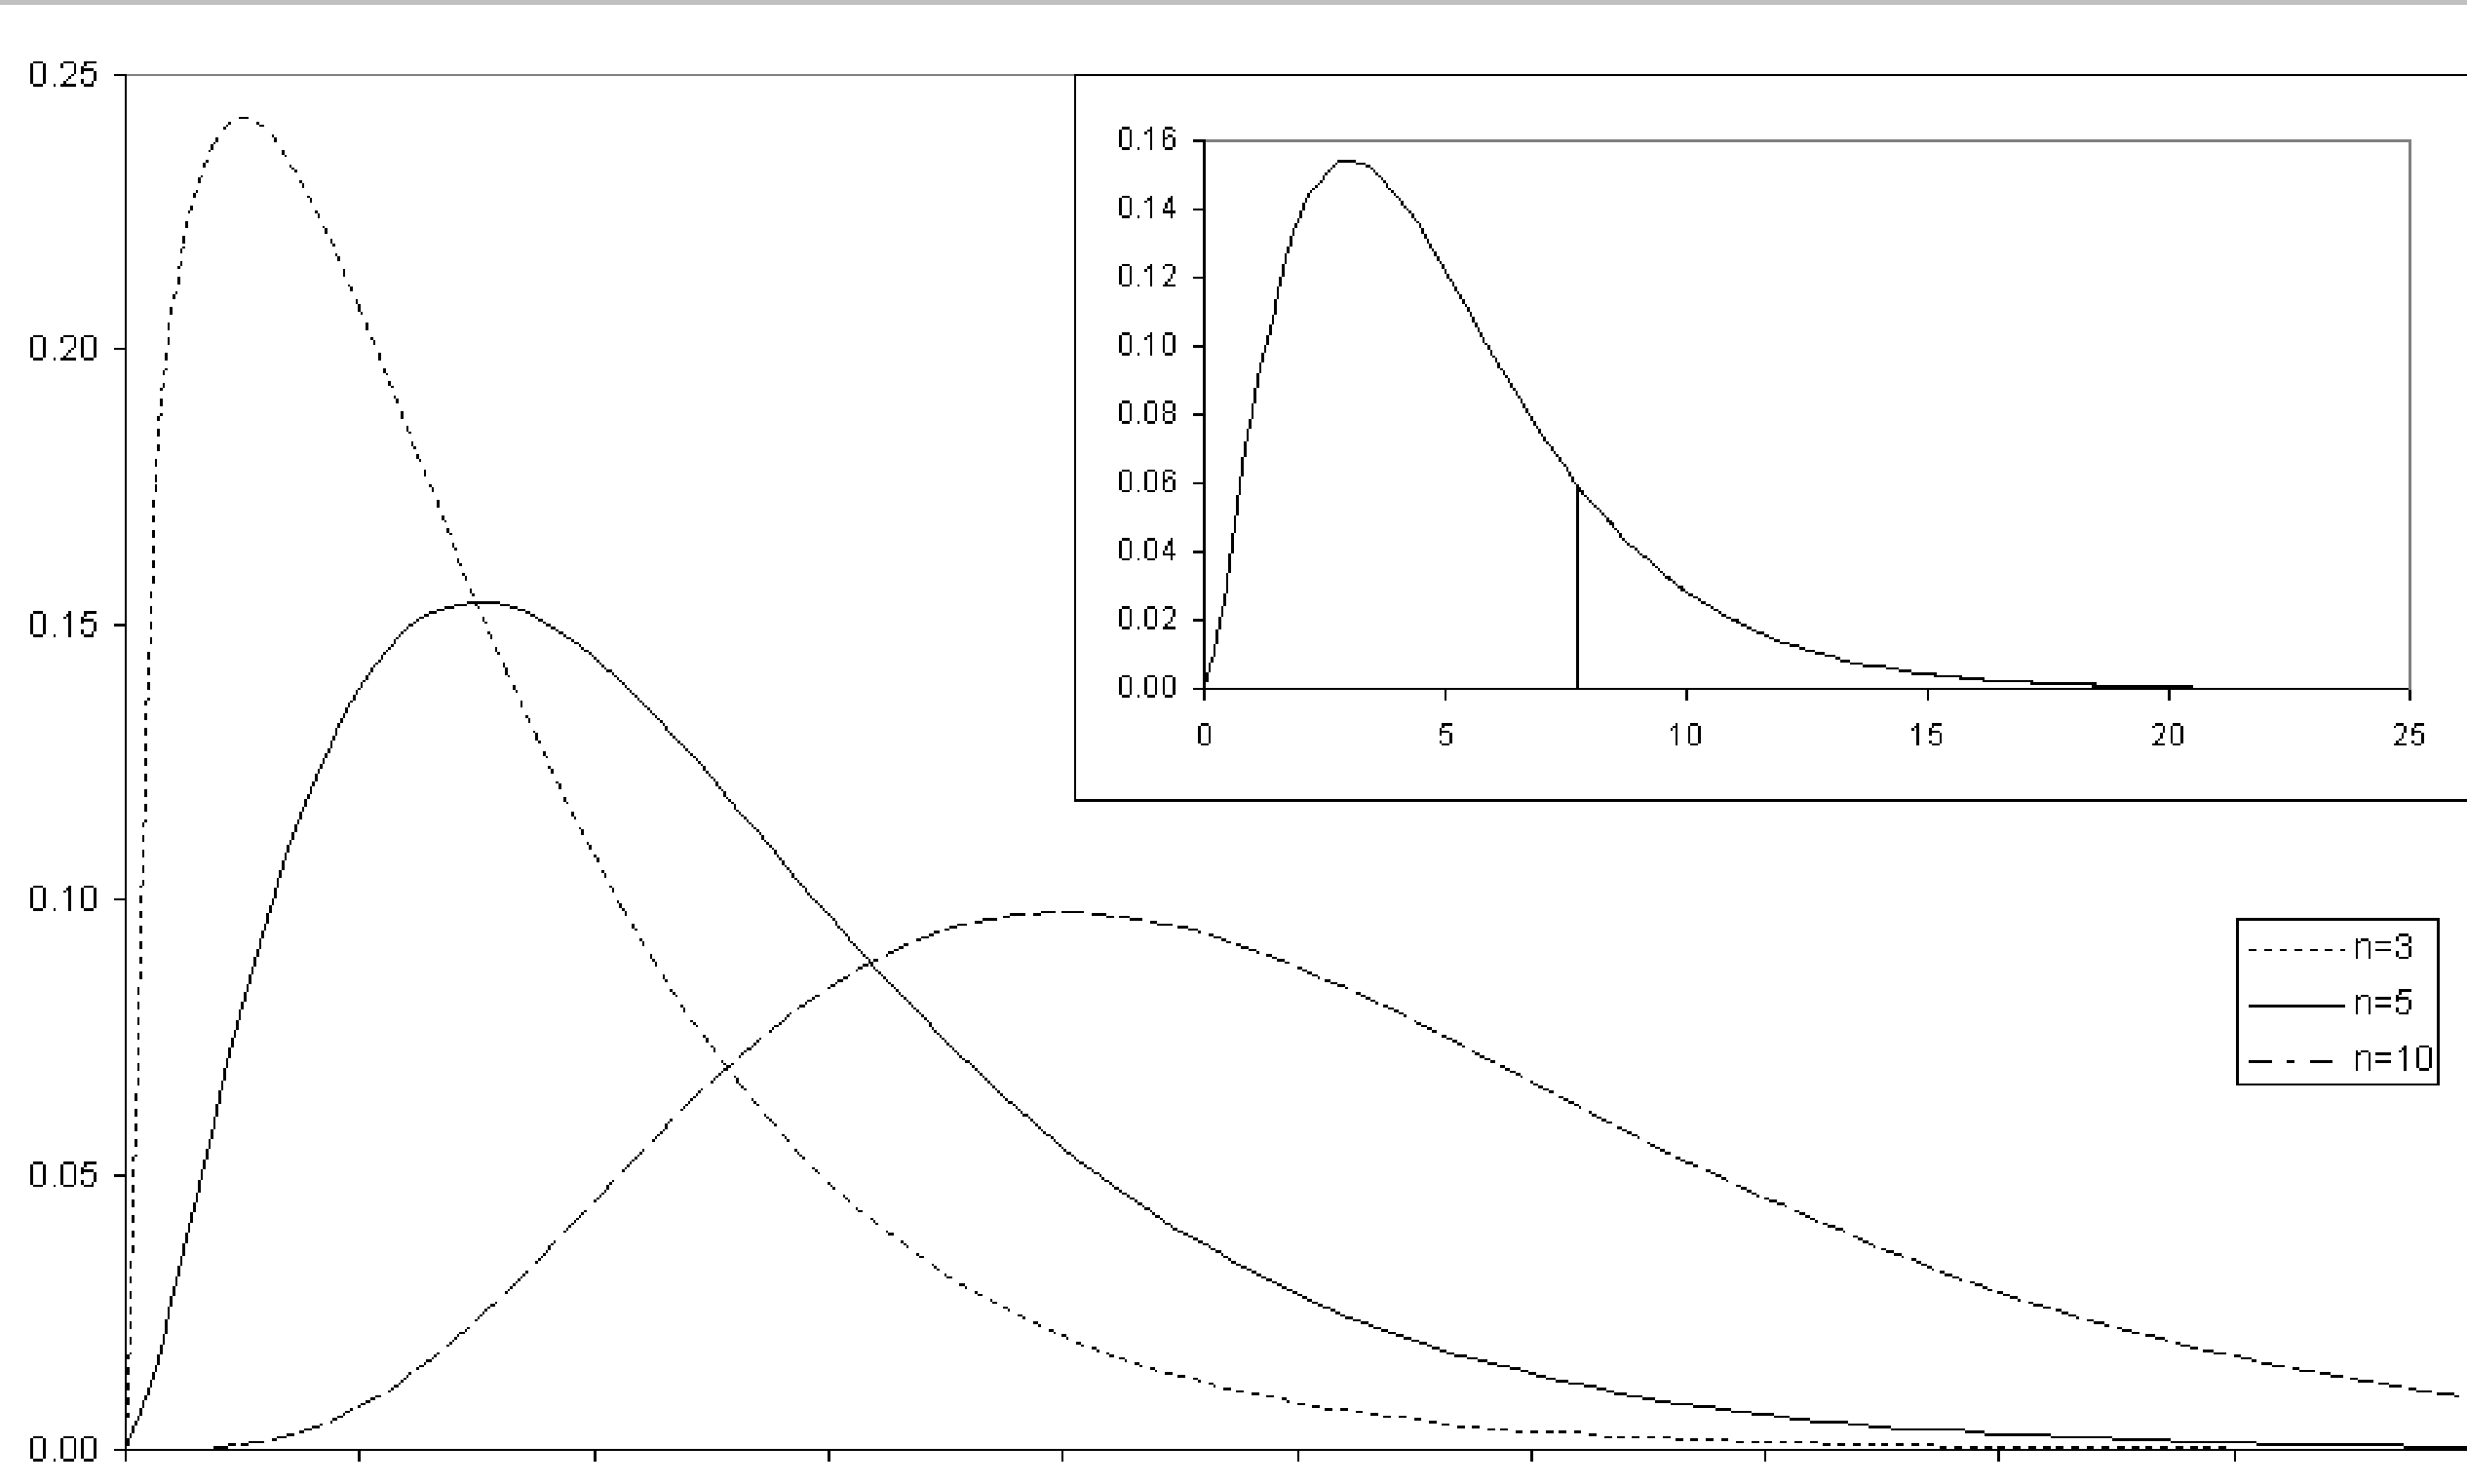
\includegraphics[width=12cm]{Figures/Chi2Distribution}
\caption{$\chi^2$ distribution for a few degrees of freedom
}\label{fig:chi2Distr}
\end{figure}


To perform a $\chi^2$-test, it is customary to evaluate the
probability of finding a value larger than the value obtained in
equations \ref{eq:defchitest} or \ref{eq:defchitestcmp}. In this
form, the result of a $\chi^2$-test gives the probability that the
set of measurements is {\textsl not} compatible with the prediction or
with another set of measurements. The confidence level of a
$\chi^2$ value is defined as the probability of finding a value
larger than $\chi^2$ expressed in percent. It is thus related to
the distribution function as follows:
\begin{equation}
  {\cl}_{S}=100\left[ 1-F\left(S\right)\right],
\end{equation}
where $S$ is the quantity defined in equation \ref{eq:defchitest}
or \ref{eq:defchitestcmp}. The confidence level corresponds to the
surface of the shaded area of the insert in the upper right corner
of figure \ref{fig:chi2Distr}.

Since the $\chi^2$ distribution is a special case of the gamma
distribution the confidence level can be expressed with the
incomplete gamma function (\cf section \ref{sec:incGamma}):
\begin{equation}
\label{eq:chiTest}
  {\cl}_{S}=100\left[ 1-\Gamma\left({S \over 2},{n\over 2}\right)\right].
\end{equation}
For large $n$ the $\chi^2$ confidence level can be computed from
the error function (\cf section \ref{sec:errorFunctionDef}):
\begin{equation}
\label{eq:chiTestAsymp}
  {\cl}_{S}=100\left[ 1-\erf\left(\sqrt{2S}-\sqrt{2n-1}\right)\right].
\end{equation}

\subsection{$\chi^2$ distribution --- Smalltalk implementation}
\marginpar{Figure \ref{fig:estimationclasses} with the box {\textbf
ChiSquaredDistribution} grayed.} Listing \ref{ls:chidist} shows
the implementation of the $\chi^2$ distribution in Smalltalk. The
asymptotic limit is implemented directly in the class creation
method.
\begin{listing} Smalltalk implementation of the $\chi^2$ distribution \label{ls:chidist}
$$\halign{ #\hfil&\quad#\hfil\cr {\sl Class}& {\Large\bf DhbChiSquareDistribution}\cr
{\sl Subclass of }&{\tt DhbGammaDistribution}\cr\noalign{\vskip 1ex}
}$$


Class methods
{\parskip 1ex\par\noindent}
{\bf degreeOfFreedom:} {\tt anInteger}
\begin{verbatim}
    ^anInteger > 40
        ifTrue: [ DhbAsymptoticChiSquareDistribution degreeOfFreedom: 
                                                            anInteger]
        ifFalse:[ super shape: anInteger / 2 scale: 2]

\end{verbatim}
{\bf distributionName}
\begin{verbatim}
    ^'Chi square distribution'
\end{verbatim}
{\bf fromHistogram:} {\tt aHistogram}
\begin{verbatim}
    | dof |
    aHistogram minimum < 0
        ifTrue: [ ^nil].
    dof := aHistogram average rounded.
    ^dof > 0 ifTrue: [ self degreeOfFreedom: aHistogram average 
                                                              rounded]
             ifFalse:[ nil ]
\end{verbatim}
{\bf shape:} {\tt aNumber1} {\bf scale:} {\tt aNumber2}
\begin{verbatim}
    ^self error: 'Illegal creation message for this class'
\end{verbatim}



Instance methods
{\parskip 1ex\par\noindent}
{\bf changeParametersBy:} {\tt aVector}
\begin{verbatim}
    super changeParametersBy: (Array with: aVector first / 2 with: 0).
\end{verbatim}
{\bf confidenceLevel:} {\tt aNumber}
\begin{verbatim}
    ^ (1 - ( self distributionValue: aNumber)) *100
\end{verbatim}
{\bf parameters}
\begin{verbatim}
    ^ Array with: alpha * 2
\end{verbatim}


\end{listing}


\subsection{Weighted point implementation}
\label{sec:weightedPoint} \marginpar{Figure
\ref{fig:estimationclasses} with the box {\textbf WeightedPoint}
grayed.} As we shall see in the rest of this chapter, the
evaluation of equation \ref{eq:defchitest} is performed at many
places. Thus, it is convenient to create a new class handling this
type of calculation.
The new class is called {\texttt PMWeightedPoint} in Smalltalk.

\noindent A weighted point has the following instance variables:
\begin{description}
  \item[\texttt xValue] the $x$ value of the data point, that is $x_i$,
  \item[\texttt yValue] the $y$ value of the data point, that is $y_i$,
  \item[\texttt weight] the weight of the point, that is $1/\sigma_i^2$
  and
  \item[\texttt error] the error of the $y$ value, that is $\sigma_i$.
\end{description}
Accessor methods for each of these instance variables are
provided. The accessor method for the error is using lazy
initialization to compute the error from the weight in case the
error has not yet been defined.

The method {\texttt chi2Contribution} --- with an added semicolon at
the end of the name for Smalltalk --- implements the computation
of one term of the sum in equation \ref{eq:defchitest}. The
argument of the method is any object implementing the behavior of
a one-variable function defined in section \ref{sec:function}.

Creating instances of the classes can be done in many ways. The
fundamental method takes as arguments $x_i$, $y_i$ and the weight
$1/\sigma_i^2$. However convenience methods are provided for
frequent cases:
\begin{enumerate}
  \item $x_i$, $y_i$ and the error on $y_i$, $\sigma_i$;
  \item $x_i$ and the content of a histogram bin; the weight is derived
  from the bin contents as explained in section \ref{sec:chitesthist};
  \item $x_i$, $y_i$ without known error; the weight of the point is set to
  1; points without error should not be used together with points
  with errors;
  \item $x_i$ and a statistical moment; in this case, the value $y_i$
  is an average over a set of measurements; the weight is determined
  from the error on the average (\cf section \ref{sec:moments});
\end{enumerate}
Examples of use of weighted points appear in many sections of this
chapter (\ref{sec:chitesthist}, \ref{sec:lsfpol},
\ref{sec:lsfnonlin}).

In the Smalltalk class {\texttt PMWeightedPoint} the values $x_i$ and
$y_i$ are always supplied as an instance of the class {\texttt Point}.
The class {\texttt PMWeightedPoint} has the following class creation
methods:
\begin{description}
  \item[\texttt point:weight:] fundamental method;
  \item[\texttt point:error:] convenience method 1;
  \item[\texttt point:count:] convenience method 2;
  \item[\texttt point:] convenience method 3
\end{description}
The convenience method 4 is implemented by the method {\texttt
asWeightedPoint} of the class {\texttt PMStatisticalMoments}. This
kind of technique is quite common in Smalltalk instead of making a
class creation method with an explicit name ({\texttt fromMoment:}
\eg).

\begin{listing} Smalltalk implementation of the weighted point class
\label{ls:weightedPoint}
$$\halign{ #\hfil&\quad#\hfil\cr {\sl Class}& {\Large\bf DhbWeightedPoint}\cr
{\sl Subclass of }&{\tt Object}\cr\noalign{\vskip 1ex}

{\sl Instance variable names:}&\parbox[t]{4 in}{\tt  xValue yValue weight error }\cr\noalign{\vskip 1ex}}$$


Class methods
{\parskip 1ex\par\noindent}
{\bf point:} {\tt aPoint}
\begin{verbatim}
    ^ self new initialize: aPoint weight: 1
\end{verbatim}
{\bf point:} {\tt aNumber} {\bf count:} {\tt anInteger}
\begin{verbatim}
    ^ self point: aNumber @ anInteger
        weight: ( anInteger > 0 ifTrue: [ 1 / anInteger]
                                ifFalse: [ 1 ])
\end{verbatim}
{\bf point:} {\tt aPoint} {\bf error:} {\tt aNumber}
\begin{verbatim}
    ^ self new initialize: aPoint error: aNumber
\end{verbatim}
{\bf point:} {\tt aPoint} {\bf weight:} {\tt aNumber}
\begin{verbatim}
    ^ self new initialize: aPoint weight: aNumber
\end{verbatim}



Instance methods
{\parskip 1ex\par\noindent}
{\bf chi2ComparisonContribution:} {\tt aWeightedPoint}
\begin{verbatim}
    ^ (aWeightedPoint yValue - yValue) squared / ( 1 / aWeightedPoint 
                                               weight + ( 1 / weight))
\end{verbatim}
{\bf chi2Contribution:} {\tt aFunction}
\begin{verbatim}
    ^ (yValue - ( aFunction value: xValue)) squared * weight
\end{verbatim}
{\bf error}
\begin{verbatim}
    error isNil
        ifTrue: [ error := 1 / weight sqrt].
    ^ error
\end{verbatim}
{\bf initialize:} {\tt aPoint} {\bf error:} {\tt aNumber}
\begin{verbatim}
    error := aNumber.
    ^ self initialize: aPoint weight: 1 / aNumber squared

\end{verbatim}
{\bf initialize:} {\tt aPoint} {\bf weight:} {\tt aNumber}
\begin{verbatim}
    xValue := aPoint x.
    yValue := aPoint y.
    weight := aNumber.
    ^ self
\end{verbatim}
{\bf point}
\begin{verbatim}
    ^ xValue @ yValue
\end{verbatim}
{\bf weight}
\begin{verbatim}
    ^ weight
\end{verbatim}
{\bf xValue}
\begin{verbatim}
    ^ xValue
\end{verbatim}
{\bf yValue}
\begin{verbatim}
    ^ yValue
\end{verbatim}


$$\halign{ #\hfil&\quad#\hfil\cr {\sl Class}& {\Large\bf DhbStatisticalMoments}\cr
{\sl Subclass of }&{\tt Object}\cr\noalign{\vskip 1ex}

{\sl Instance variable names:}&\parbox[t]{4 in}{\tt  moments }\cr\noalign{\vskip 1ex}}$$


Instance methods
{\parskip 1ex\par\noindent}
{\bf asWeightedPoint:} {\tt aNumber}
\begin{verbatim}
    ^DhbWeightedPoint point: aNumber @ self average error: self 
                                                        errorOnAverage
\end{verbatim}


\end{listing}

\section{$\chi^2$-test on histograms}
\label{sec:chitesthist} As we have seen in section
\ref{sec:histogram} histograms are often used to collect
experimental data. Performing a $\chi^2$-test of data accumulated
into a histogram against a function is a frequent task of data
analysis.

The $\chi^2$ statistics defined by equation \ref{eq:defchitest}
requires an estimate of the standard deviation of the content of
each bin. One can show that the contents of a histogram bin is
distributed according to a Poisson distribution. The Poisson
distribution is a discrete distribution\footnote{A discrete
distribution is a probability distribution whose random variable
is an integer.} whose average is equal to the variance. The
probability of observing the integer $k$ is defined by:
\begin{equation}
 P_{\mu}\left(k\right)= {\mu^k\over k!}e^{\mu},
\end{equation}
where $\mu$ is the average of the distribution. In the case of a
histogram, the estimated variance of the bin content is then the
bin content itself. Therefore equation \ref{eq:defchitest}
becomes:
\begin{equation}
\label{eq:defchitesthist}
  S=\sum_{i=1}^n
  { \left\{n_i - \mu\left[x_{\min} + \left(i+{1\over 2} \right)w\right]\right\}^2 \over
  n_i},
\end{equation}
where $n$ is the number of bins of the histogram, $x_{\min}$ its
minimum and $w$ its bin width. The estimation of the bin content
against which the $\chi^2$ statistics is computed, $\mu$, is now a
function evaluated at the middle of each bin to average out
variations of the function over the bin interval.

In fact, the function $\mu$ is often related to a probability
density function since histograms are measuring probability
distributions. In this case the evaluation is somewhat different.
Let $P\left(x\right)$ be the probability density function against
which the $\chi^2$ statistics is computed. Then, the predicted bin
content for bin $i$ is given by:
\begin{equation}
\label{eq:probbincontents}
 \mu_i = wNP\left[x_{\min} + \left(i+{1\over 2} \right)w\right],
\end{equation}
where $N$ is the total number of values accumulated in the
histogram. This is a symmetric version of the definition of a
probability density function: $w$ plays the role of $dx$ in
equation \ref{eq:probdensity}. Plugging equation
\ref{eq:probbincontents} into equation \ref{eq:defchitesthist}
yields the expression of the $\chi^2$ statistics for a histogram
computed against a probability density function $P\left(x\right)$:
\begin{equation}
\label{eq:defchitesthistprob}
  S=\sum_{i=1}^n
  { \left\{n_i - wNP\left[x_{\min} + \left(i+{1\over 2} \right)w\right]\right\}^2 \over
  n_i},
\end{equation}
This equation cannot be applied for empty bins. If the bin is
empty one can set the weight to 1. This corresponds to a $63\%$
probability of observing no counts if the expected number of
measurement is larger than 0.

In both implementations a single class is in charge of evaluating
the predicted bin contents. This class is called a scaled
probability density function. It is defined by a probability
distribution and a histogram.

\subsection{$\chi^2$-test on histograms --- Smalltalk implementation}
\marginpar{Figure \ref{fig:estimationclasses} with the box {\textbf
ScaledProbabilityDistribution} grayed.} Listing
\ref{ls:scaleddist} shows the implementation of a scaled
probability density function in Smalltalk. Listing
\ref{ls:chitesthist} shows the additional methods for the class
{\texttt PMHistogram} needed to perform a $\chi^2$-test. Examples of
use are given in sections \ref{sec:slsfnonlin} and
\ref{sec:smlfhist}. Here is a simple example showing how to
compute a $\chi^2$-confidence level to estimate the goodness of a
random number generator.
\begin{displaycode}{Smalltalk}
\label{exs:chitest}
 | trials probDistr histogram |
 trials := 5000.
 probDistr := PMNormalDistribution new.
 histogram := PMHistogram new.
 histogram freeExtent: true; setDesiredNumberOfBins: 100.
 trials timesRepeat: [ histogram accumulate: probDistr random ].
 histogram chi2ConfidenceLevelAgainst:
        ( PMScaledProbabilityDensityFunction histogram: histogram
                                          against: probDistr)
\end{displaycode}
The first line after the declaration defines the number of data to
be generated to 5000. After, an new instance of a probability
distribution --- in this case a normal distribution with average 0
and variance 1 --- is created. Then, a new instance of a histogram
is created and the next line defines it with a rough number of
bins of 100 and the ability to automatically adjust its limits.
After all instances have been created, random data generated by
the probability distribution are generated. The last statement
--- extending itself over the last three lines --- calculates
the confidence level. The argument of the method {\texttt
chi2ConfidenceLevelAgainst:} is a scaled probability distribution
constructed over the histogram and the probability distribution
used to generate the accumulated data.

The class {\texttt PMScaledProbabilityDensityFunction} has two class
creation methods. The class method {\texttt histogram:against:} takes
two arguments, a histogram and a probability distribution. This
method is used to perform a $\chi^2$-test of the specified
histogram against the given probability distribution. The class
method {\texttt histogram:distributionClass:} first create a
probability distribution of the given class using parameters
estimated from the histogram. This method is used to create a
scaled probability density function whose parameters will be
determined with least square or maximum likelihood fits.

\begin{listing} Smalltalk implementation of a scaled
probability density function \label{ls:scaleddist}
$$\halign{ #\hfil&\quad#\hfil\cr {\sl Class}& {\Large\bf DhbScaledProbabilityDensityFunction}\cr
{\sl Subclass of }&{\tt Object}\cr\noalign{\vskip 1ex}

{\sl Instance variable names:}&\parbox[t]{4 in}{\tt  probabilityDensityFunction count binWidth }\cr\noalign{\vskip 1ex}}$$


Class methods
{\parskip 1ex\par\noindent}
{\bf histogram:} {\tt aHistogram} {\bf against:} {\tt aProbabilityDensityFunction}
\begin{verbatim}
    ^ self new 
        initialize: aProbabilityDensityFunction
        binWidth: aHistogram binWidth
        count: aHistogram totalCount
\end{verbatim}
{\bf histogram:} {\tt aHistogram} {\bf distributionClass:} {\tt aProbabilityDensityFunctionClass}
\begin{verbatim}
    ^ (aProbabilityDensityFunctionClass fromHistogram: aHistogram) 
        ifNotNil: [:dp | self histogram: aHistogram against: dp]
\end{verbatim}

Instance methods
{\parskip 1ex\par\noindent}
{\bf changeParametersBy:} {\tt aVector}
\begin{verbatim}
    count := count + aVector last.
    probabilityDensityFunction changeParametersBy: aVector.
\end{verbatim}
{\bf distributionFunction}
\begin{verbatim}
    ^probabilityDensityFunction distributionFunction
\end{verbatim}
{\bf initialize:} {\tt aProbabilityDensityFunction} {\bf binWidth:} {\tt aNumber} {\bf count:} {\tt anInteger}
\begin{verbatim}
    probabilityDensityFunction := aProbabilityDensityFunction.
    binWidth := aNumber.
    count := anInteger.
    ^ self
\end{verbatim}
{\bf parameters}
\begin{verbatim}
    ^ probabilityDensityFunction parameters copyWith: count
\end{verbatim}
{\bf printOn:} {\tt aStream}
\begin{verbatim}
    super printOn: aStream.
    aStream nextPut: $[;
            nextPutAll: probabilityDensityFunction class 
                                                     distributionName;
            nextPut: $].
\end{verbatim}
{\bf setCount:} {\tt aNumber}
\begin{verbatim}
    count := aNumber.
\end{verbatim}
{\bf value:} {\tt aNumber}
\begin{verbatim}
    ^ (probabilityDensityFunction value: aNumber) * binWidth * count
\end{verbatim}
{\bf valueAndGradient:} {\tt aNumber}
\begin{verbatim}
    | g temp |
    g := probabilityDensityFunction valueAndGradient: aNumber.
    temp := binWidth * count.
    ^ Array with: g first * temp
           with: ( (g last collect: [:each | each * temp]) copyWith: 
                                                   g first * binWidth)
\end{verbatim}


\end{listing}

The evaluation of equation \ref{eq:defchitesthistprob} is
performed by the method {\texttt chi2Against:} of the class {\texttt
PMHistogram}. This method uses the iterator method {\texttt
pointsAndErrorsDo:}. This method iterates on all bins and performs
on each of them a block using as argument a weighted point as
described in section \ref{sec:weightedPoint}. This iterator method
is also used for least square and maximum likelihood fits (\cf
sections \ref{sec:slsfnonlin} and \ref{sec:smlfhist}).

\begin{listing} Smalltalk implementation of $\chi^2$-test on histograms \label{ls:chitesthist}
$$\halign{ #\hfil&\quad#\hfil\cr {\sl Class}& {\Large\bf DhbHistogram}\cr
{\sl Subclass of }&{\tt Object}\cr\noalign{\vskip 1ex}

{\sl Instance variable names:}&\parbox[t]{4 in}{\tt  minimum binWidth overflow underflow moments contents freeExtent cacheSize desiredNumberOfBins }\cr\noalign{\vskip 1ex}}$$


Instance methods
{\parskip 1ex\par\noindent}
{\bf chi2Against:} {\tt aScaledDistribution}
\begin{verbatim}
    | chi2 |
    chi2 := 0.
    self pointsAndErrorsDo:
        [ :each | chi2 := ( each chi2Contribution: 
                                         aScaledDistribution) + chi2 ].
    ^ chi2

\end{verbatim}
{\bf chi2ConfidenceLevelAgainst:} {\tt aScaledDistribution}
\begin{verbatim}
    ^ (DhbChiSquareDistribution degreeOfFreedom: ( contents size - 
                                 aScaledDistribution parameters size))
            confidenceLevel: ( self chi2Against: aScaledDistribution)
\end{verbatim}
{\bf pointsAndErrorsDo:} {\tt aBlock}
\begin{verbatim}
    | x |
    x := self minimum - ( self binWidth / 2).
    contents do:
        [ :each |
          x := x + self binWidth.
          aBlock value: ( DhbWeightedPoint point: x count: each).
        ].
\end{verbatim}


\end{listing}

\section{Definition of estimation}
Let us assume that an observable quantity $y$ is following a
probability distribution described by a set of observable
quantities $x_1,x_2\ldots$ - called the experimental conditions -
and a set of parameters $p_1,p_2\ldots$.
In other words, the robability density function of the random variable\footnote{For
simplicity we shall use the same notation for the random variable
and the observable quantity.} corresponding to the observable
quantity $y$ can be written as
\begin{equation}
\label{eq:estimprob}
  P\left(y\right)=P\left(y;{\textbf x},{\textbf p}\right),
\end{equation}
where ${\textbf x}$ is the vector $\left(x_1,x_2\ldots\right)$ and
${\textbf p}$ the vector $\left(p_1,p_2\ldots\right)$.

The estimation of the values of the parameters $p_1,p_2\ldots$ is
the determination of the parameters $p_1,p_2\ldots$ by performing
several measurements of the observable $y$ for different
experimental conditions $x_1,x_2\ldots$.

Let $N$ be the number of measurements; let $y_i$ be the $\mbox{\textrm
i}^{\mbox{\textrm th}}$ measured value of the observable $y$ under the
experimental conditions ${\textbf x}_i$.

\subsection{Maximum likelihood estimation}
\label{sec:mlf} The maximum likelihood estimation of the
parameters ${\textbf p}$ is the set of values $\bar{\textbf p}$ maximizing
the following function:
\begin{equation}
\label{eq:maxlike}
  L\left({\textbf p}\right)=\prod_{i=1}^N P\left(y_i;{\textbf x}_i,{\textbf p}\right)
\end{equation}
By definition the likelihood function $L\left({\textbf p}\right)$ is
the probability of making the $N$ measurements. The maximum
likelihood estimation determines the estimation $\bar{\textbf p}$ of
the parameters ${\textbf p}$ such that the series of measurements
performed is the most probable, hence the name maximum likelihood.

One can show that the maximum likelihood estimation is robust and
unbiased. The robustness and the bias of an estimation are defined
mathematically. For short, {\textsl robust} means that the estimation
converges toward the true value of the parameters for an infinite
number of measurements; {\textsl unbiased} means that the deviations
between the estimated parameters and their true value are
symmetrically distributed around 0 for any finite number of
measurements.

Equation \ref{eq:maxlike} is often rewritten in logarithmic form
to ease the computation of the likelihood function.
\begin{equation}
\label{eq:logmaxlike}
  I\left({\textbf p}\right)=\ln L\left({\textbf p}\right)=\sum_{i=1}^N\ln P\left(y_i;{\textbf x}_i,{\textbf p}\right)
\end{equation}
The function $I\left({\textbf p}\right)$ is related to information and
is used in information theory.

\subsection{Least square estimation}
Let us assume that the random variable $y$ is distributed
according to a normal distribution of given standard deviation
$\sigma$ and that the average of the normal distribution is given
by a function $F\left({\textbf x},{\textbf p}\right)$ of the experimental
conditions and the parameters. In this case equation
\ref{eq:estimprob} becomes:
\begin{equation}
\label{eq:estimprobnorm}
  P\left(y\right)={1\over\sqrt{2\pi\sigma^2}}e^{-{
  \left[y-F\left({\textbf x},{\textbf p}\right)\right]^2\over 2\sigma^2}}
\end{equation}
Plugging equation \ref{eq:estimprobnorm} into equation
\ref{eq:logmaxlike} yields:
\begin{equation}
  I\left({\textbf p}\right)=-N\sqrt{2\pi\sigma^2}-
  \sum_{i=1}^N {
  \left[y-F\left({\textbf x},{\textbf p}\right)\right]^2\over 2\sigma^2}
\end{equation}
The problem of finding the maximum of $I\left({\textbf p}\right)$ is
now equivalent to the problem of finding the minimum of the
function:
\begin{equation}
\label{eq:lsmlestim}
  S_{\mathop{ML}}\left({\textbf p}\right)=\sum_{i=1}^N {
  \left[y-F\left({\textbf x},{\textbf p}\right)\right]^2\over \sigma^2},
\end{equation}
where a redundant factor 2 has been removed. This kind of
estimation is called least square estimation. Written as in
equation \ref{eq:lsmlestim} least square estimation is fully
equivalent to maximum likelihood estimation. By definition, the
quantity $S_{\mathop{ML}}\left({\textbf p}\right)$ is distributed as a
$\chi^2$ random variable with $N-m$ degrees of freedom where $m$
is the number of parameters, that is the dimension of the vector
${\textbf p}$.

In practice, however, the standard deviation $\sigma$ is not known
and frequently depends on the parameters ${\textbf p}$. In that case,
one uses instead an estimation for the standard deviation. Either
the standard deviation of each measurement is determined
experimentally by making several measurements under the same
experimental conditions or it is estimated from the measurement
error. Then, equation \ref{eq:lsmlestim} can be rewritten as:
\begin{equation}
\label{eq:lsestim}
  S\left({\textbf p}\right)=\sum_{i=1}^N {
  \left[y-F\left({\textbf x},{\textbf p}\right)\right]^2\over \sigma_i^2}.
\end{equation}
The least square estimation is obtained by minimizing the quantity
$S\left({\textbf p}\right)$ with respect to the parameters ${\textbf p}$.
This kind of estimation can be used to determine the parameters of
a functional dependence of the variable $y$ from the observable
quantities ${\textbf x}$. For this reason it is also called a least
square fit when it is used to fit the parameter of a functional
dependence to the measurements.

In general the distribution of the random variable $y$ may not be
a normal distribution. One can nevertheless show that the least
square estimation is robust. However, it is biased. Depending on
the nature of the distribution of the random variable $y$ the
parameters may be over- or underestimated. This is especially the
case when working with histograms.

We have said that all measurements of the observable quantities
$y$ must be distributed according to a normal distribution so that
the quantity $S\left({\textbf p}\right)$ of equation \ref{eq:lsestim}
is distributed as a $\chi^2$ random variable. In general this is
often the case\footnote{This is a consequence of a theorem known
as the law of large numbers.} when dealing with a large quantity
of measurements. Thus, a least square fit is also called a
$\chi^2$ fit. In this case one can apply the $\chi^2$-test
described in section \ref{sec:chitest} to assess the goodness of
the fitted function.

If $S\left({\textbf p}\right)$ has a minimum respective to ${\textbf p}$
then all partial derivatives of the function $S\left({\textbf
p}\right)$ respective to each of the components of the vector
${\textbf p}$ are zero. Since the function is positive and quadratic
in ${\textbf p}$, it is clear that the function must have at least one
minimum. Under this circumstances the minimum can be obtained by
solving the following set of equations:
\begin{equation}
\label{eq:lsderiv}
  {\displaystyle \partial\over\displaystyle\partial p_j}
  F\left({\textbf x}_i;p_1,\ldots,p_m\right)=0\mbox{\quad for $j=1,\ldots,m$}
\end{equation}
where $m$ is the number of parameters, that is the dimension of
the vector ${\textbf p}$. When a solution is found, one should in
principle verify that it is really a minimum. Solving equation
\ref{eq:lsderiv} gives the following system of equations:
\begin{equation}
\label{eq:lsequs}
  \sum_{i=1}^N {
  y-F\left({\textbf x},{\textbf p}\right)\over \sigma_i^2}\cdot
  {\displaystyle \partial\over\displaystyle\partial p_j} S\left(p_1,\ldots,p_m\right)
  =0\mbox{\quad for $j=1,\ldots,m$}
\end{equation}
Once the system above has been solved, one can compute the value
of $S\left({\textbf p}\right)$ using equations \ref{eq:lsestim} or,
better, the value $S_{\mathop{ML}}\left({\textbf p}\right)$ using
equation \ref{eq:lsmlestim}. Computing the $\chi^2$ confidence
level of that value (\cf section \ref{sec:chitest}) using a
$\chi^2$ distribution with $N-m$ degrees of freedom gives the
probability that the fit is acceptable.

\section{Least square fit with linear dependence}
\label{eq:lslinear} If the function $F\left({\textbf x},{\textbf
p}\right)$ is a linear function of the vector ${\textbf p}$, it can be
written in the following form:
\begin{equation}
  F\left({\textbf x},{\textbf p}\right)=\sum_{j=1}^m f_j\left({\textbf
  x}\right)\cdot p_j.
\end{equation}
In that case, equation \ref{eq:lsequs} become a system of linear
equations of the form:
\begin{equation}
\label{eq:lsmequs}
{\textbf M}\cdot{\textbf p}={\textbf c},
\end{equation}
where the coefficients of the matrix ${\textbf M}$ are given by:
\begin{equation}
  M_{jk}=\sum_{i=1}^N {\displaystyle f_j\left({\textbf x}_i\right)f_k\left({\textbf x}_i\right)
  \over\displaystyle \sigma_i^2}\mbox{\quad for $j,k=1,\ldots,m$},
\end{equation}
and the components of the constant vector ${\textbf c}$ are given by:
\begin{equation}
  c_j=\sum_{i=1}^N {\displaystyle y_if_j\left({\textbf x}_i\right)
  \over\displaystyle \sigma_i^2}\mbox{\quad for $j=1,\ldots,m$}.
\end{equation}
Equation \ref{eq:lsmequs} is a system of linear equation which can
be solved according to the algorithms exposed in sections
\ref{sec:lineqs} and \ref{sec:lup}. If one is interested only in
the solution this is all there is to do.

A proper fit, however, should give an estimation of the error in
estimating the parameters. The inverse of the matrix ${\textbf M}$ is
the error matrix for the fit. The error matrix is used to compute
the estimation of variance on the function $F\left({\textbf x},{\textbf
p}\right)$ as follows:
\begin{equation}
\label{eq:fitError}
  \var\left[F\left({\textbf x},{\textbf p}\right)\right]=\sum_{j=1}^m \sum_{k=1}^m
  M_{jk}^{-1}f_j\left({\textbf x}\right)f_k\left({\textbf x}\right).
\end{equation}
The estimated error on the function $F\left({\textbf x},{\textbf
p}\right)$ is the square root of the estimated variance.

The diagonal elements of the error matrix are the variance of the
corresponding parameter. That is:
\begin{equation}
\var\left(p_j\right)=M_{jj}^{-1}\mbox{\quad for $j=1,\ldots,m$}.
\end{equation}
The off diagonal elements describe the correlation between the
errors on the parameters. One defines the correlation coefficient
of parameter $p_j$ and $p_j$ by:
\begin{equation}
  \cor\left(p_j,p_k\right)={\displaystyle M_{jk}^{-1}
  \over\displaystyle\sqrt{M_{jj}^{-1}M_{kk}^{-1}}}\mbox{\quad for
$j,k=1,\ldots,m$ and $j\ne k$}.
\end{equation}
All correlation coefficients are comprised between -1 and 1. If
the absolute value of a correlation coefficient is close to 1, it
means that one of the two corresponding two parameters is
redundant for the fit. In other word, one parameter can be
expressed as a function of the other.

\section{Linear regression}
A linear regression is a least square fit with a linear function
of a single variable.
The dimension of the vector ${\textbf x}$ is one
and the dimension of the vector ${\textbf p}$ is two. The function to
fit has only two parameters. The following convention is standard:
\begin{equation}
  \left\{
  \begin{array}{lcl}
    p_1 & = & a, \\
    p_2 & = & b, \\
    F\left({\textbf x},{\textbf p}\right)&=&ax+b.
  \end{array}
  \right.
\end{equation}
With these definitions, the system of equations \ref{eq:lsmequs}
becomes:
\begin{equation}
\label{eq:linreg}
  \left\{
  \begin{array}{lcl}
    \displaystyle \sum_{i=1}^N {\displaystyle x_i^2\over\displaystyle\sigma^2}a
    + \sum_{i=1}^N {\displaystyle x_i\over\displaystyle\sigma^2}b& = &
    \displaystyle\sum_{i=1}^N {\displaystyle x_i y_i\over\displaystyle\sigma^2}
    \\*[4ex]
    \displaystyle\sum_{i=1}^N {\displaystyle x_i\over\displaystyle\sigma^2}a
    + \sum_{i=1}^N {\displaystyle 1\over\displaystyle\sigma^2}b& = &
    \displaystyle\sum_{i=1}^N {\displaystyle y_i\over\displaystyle\sigma^2}.
  \end{array}
  \right.
\end{equation}
This system can easily be solved. Before giving the solution, let
us introduce a short hand notation for the weighted sums:
\begin{equation}
\braket{Q} = \sum_{i=1}^N {\displaystyle
Q_i\over\displaystyle\sigma^2_i}.
\end{equation}
Using this notation the solution of the system of equations
\ref{eq:linreg} can be written as:
\begin{equation}
  \left\{
  \begin{array}{lcl}
    a& = & {\displaystyle\braket{xy}\cdot\braket{1}-\braket{x}\cdot\braket{y}
       \over\displaystyle\braket{xx}\cdot\braket{1}-\braket{x}\cdot\braket{x}}
    \\*[3ex]
    b& = & {\displaystyle\braket{xx}\cdot\braket{y}-\braket{xy}\cdot\braket{x}
       \over\displaystyle\braket{xx}\cdot\braket{1}-\braket{x}\cdot\braket{x}}
  \end{array}
  \right.
\end{equation}
where the symmetry of the expression is quite obvious. It is
interesting to note that if we had fitted $x$ as a linear function
of $y$, that is $x=\tilde{a}y+\tilde{b}$, we would have the
following expression for the slope:
\begin{equation}
\tilde{a}=
{\displaystyle\braket{xy}\cdot\braket{1}-\braket{x}\cdot\braket{y}
       \over\displaystyle\braket{yy}\cdot\braket{1}-\braket{y}\cdot\braket{y}}.
\end{equation}
If the dependence between $x$ and $y$ is truly a linear function,
the product $a\tilde{a}$ ought to be 1. The square root of the
product $a\tilde{a}$ is defined as the correlation coefficient of
the linear regression, the sign of the square root being the sign
of the slope. The correlation coefficient $r$ is thus given by:
\begin{equation}
\label{eq:corrcoeff}
r={\displaystyle\braket{xy}\cdot\braket{1}-\braket{x}\cdot\braket{y}
  \over\displaystyle\sqrt{\left(\braket{xx}\cdot\braket{1}-\braket{x}\cdot\braket{x}\right)
  \left(\braket{yy}\cdot\braket{1}-\braket{y}\cdot\braket{y}\right)}}.
\end{equation}
Since the least square fit is a biased estimator for the
parameters, the square of the correlation coefficient is less than
1 in practice. The value of the correlation coefficient lies
between -1 and 1. A good linear fit ought to have the absolute
value of $r$ close to 1.

Finally the error matrix of a linear regression is given by:
\begin{equation}
{\textbf M}^{-1}={\displaystyle 1
\over\displaystyle\braket{xx}\cdot\braket{1}-\braket{x}\cdot\braket{x}}
\pmatrix{\braket{xx}&-\braket{x}\cr-\braket{x}&\braket{1}\cr}
\end{equation}
when the vector representing the parameters of the fit is defined
as $\left(b,a\right)$ in this order.

When fitting a functional dependence with one variable, $x$ and
many parameters, one can use a linear regression to reduce
rounding errors when the observed values $y_1,\ldots,y_N$ cover a
wide numerical range. Let $a$ and $b$ be the result of the linear
regression of the values $y_i$ as a function of $x_i$. One defines
the new quantity $y^{\prime}_i = y_i -\left(a x_i+b\right)$ for
all $i$. The standard deviation of $y^{\prime}_i$ is the same as
that of $y_i$ since the subtracted expression is just a change of
variable. In fact, the linear regression does not need to be a
good fit at all. Then, the functional dependence can be fitted on
the quantities $y^{\prime}_1,\ldots,y^{\prime}_N$. We shall give a
detailed example on this method in section \ref{sec:lsfpol}

\subsection{Linear regression --- General  implementation}
\marginpar{Figure \ref{fig:estimationclasses} with the box {\textbf
LinearRegression} grayed.} Linear regression is implemented within
a single class using a similar implementation as that of the
statistical moments.
This means that individual measurements are
accumulated and not stored.
The drawback is that the object cannot
compute the confidence level of the fit.
This is not so much a
problem since the correlation coefficient is usually sufficient to
estimate the goodness of the fit.

\noindent The class has the following instance variables:
\begin{description}
  \item[\texttt sum1] is used to accumulate the sum of weights, that
  is, $\braket{1}$,
  \item[\texttt sumX] is used to accumulate the weighted sum of $x_i$, that
  is, $\braket{x}$,
  \item[\texttt sumY] is used to accumulate the weighted sum of $y_i$, that
  is, $\braket{y}$,
  \item[\texttt sumXY] is used to accumulate the weighted sum of $x_i\times y_i$, that
  is, $\braket{xy}$,
  \item[\texttt sumXX] is used to accumulate the weighted sum of $x_i^2$, that
  is, $\braket{xx}$,
  \item[\texttt sumYY] is used to accumulate the weighted sum of $y_i^2$, that
  is, $\braket{yy}$,
  \item[\texttt slope] the slope of the linear regression, that is,
  $a$,
  \item[\texttt intercept] the value of the linear regression at $x=0$, that is,
  $b$,
  \item[\texttt tt correlationCoefficient] the correlation coefficient, that is,
  $r$ in equation \ref{eq:corrcoeff}.
\end{description}
When either one of the instance variables {\texttt slope}, {\texttt
intercept} or {\texttt correlationCoefficient} is needed, the method
{\texttt computeResults} calculating the values of the three instance
variables is called using lazy initialization.
When new data is added to the object, these variables are reset.
It is thus
possible to investigate the effect of adding new measurements on
the results.

The methods {\texttt asPolynomial} and {\texttt asEstimatedPolynomial}
return an object used to compute the predicted value for any $x$.
The estimated polynomial is using the error matrix of the least
square fit to compute the error on the predicted value. Estimated
polynomials are explained in section \ref{sec:lsfpol}

\subsection{Linear regression --- Smalltalk  implementation}
Listing \ref{ls:linreg} shows the complete implementation in
Smalltalk. The following code shows how to use the class {\texttt
PMLinearRegression} to perform a linear regression over a series
of measurements .
\begin{displaycode}{Smalltalk}

 | linReg valueStream measurement slope intercept
   correlationCoefficient estimation value error|
 linReg := PMLinearRegression new.
 [ valueStream atEnd ]
        whileFalse: [ measurement := valueStream next.
                     linReg addPoint: measurement point
                              weight: measurement weight ].
 slope := linReg slope.
 intercept := linReg intercept.
 correlationCoefficient := linReg correlationCoefficient.
 estimation := linReg asEstimatedPolynomial.
 value := estimation value: 0.5.
 error := estimation error: 0.5.
\end{displaycode}
This example assumes that the measurement of the random variable
are obtained from a stream. The exact implementation of the stream
is not shown here. The first line after the declaration creates a
new instance of class {\texttt DhbLinearRegression}. Next comes the
loop over all values found in the stream. This examples assumes
that the values are stored on the stream as a single object
implementing the following methods:
\begin{description}
  \item[\texttt point] returns a point containing the measurement,
  that is, the pair $\left(x_i,y_i\right)$ for all $i$,
  \item[\texttt weight] returns the weight of the measurement, that
  is, $1/\sigma^2_i$.
\end{description}
\noindent Each point is accumulated into the linear regression
object with the method {\texttt addPoi©nt:weight:}.

After all measurements have been read, the results of the linear
regression are fetched.
The last three lines show how to obtain a
polynomial object used to compute the value predicted by the
linear regression at $x=0.5$ and the error on that prediction.

The mechanism of lazy initialization is implemented by setting the
three instance variables {\texttt slope}, {\texttt intercept} and {\texttt
correlationCoefficient} to {\texttt nil} in the method {\texttt reset}.

\begin{listing}[label=ls:linreg]{Smalltalk}
  {Smalltalk implementation of linear regression}
XXX
  % $$\halign{ #\hfil&\quad#\hfil\cr {\sl Class}& {\Large\bf DhbLinearRegression}\cr
{\sl Subclass of }&{\tt Object}\cr\noalign{\vskip 1ex}

{\sl Instance variable names:}&\parbox[t]{4 in}{\tt  sum1 sumX sumY sumXX sumYY sumXY slope intercept correlationCoefficient }\cr\noalign{\vskip 1ex}}$$


Class methods
{\parskip 1ex\par\noindent}
{\bf new}
\begin{verbatim}
    ^ super new reset; yourself
\end{verbatim}

Instance methods
{\parskip 1ex\par\noindent}
{\bf add:} {\tt aPoint}
\begin{verbatim}
    self add: aPoint weight: 1.
\end{verbatim}
{\bf add:} {\tt aPoint} {\bf weight:} {\tt aNumber}
\begin{verbatim}
    sum1 := sum1 + aNumber.
    sumX := sumX + (aPoint x * aNumber).
    sumY := sumY + (aPoint y * aNumber).
    sumXX := sumXX + (aPoint x squared * aNumber).
    sumYY := sumYY + (aPoint y squared * aNumber).
    sumXY := sumXY + (aPoint x * aPoint y * aNumber).
    self resetResults
\end{verbatim}
{\bf asEstimatedPolynomial}
\begin{verbatim}
    ^ (DhbEstimatedPolynomial coefficients: self coefficients)
            errorMatrix: self errorMatrix;
            yourself
\end{verbatim}
{\bf asPolynomial}
\begin{verbatim}
    ^ DhbPolynomial coefficients: self coefficients
\end{verbatim}
{\bf coefficients}
\begin{verbatim}
    ^ Array with: self intercept with: self slope
\end{verbatim}
{\bf computeResults}
\begin{verbatim}
    | xNorm xyNorm |
    xNorm := sumXX * sum1 - (sumX * sumX).
    xyNorm := sumXY * sum1 - (sumX * sumY).
    slope := xyNorm / xNorm.
    intercept := (sumXX * sumY - (sumXY * sumX)) / xNorm.
    correlationCoefficient := xyNorm 
                / (xNorm * (sumYY * sum1 - (sumY * sumY))) sqrt
\end{verbatim}
{\bf correlationCoefficient}
\begin{verbatim}
    correlationCoefficient isNil
        ifTrue: [ self computeResults].
    ^ correlationCoefficient
\end{verbatim}
{\bf errorMatrix}
\begin{verbatim}
    | c1 cx cxx |
    c1 := 1.0 / (sumXX * sum1 - sumX squared).
    cx := sumX negated * c1.
    cxx := sumXX * c1.
    c1 := sum1 * c1.
    ^ DhbSymmetricMatrix rows: (Array with: (Array with: cxx with: cx)
                with: (Array with: cx with: c1))
\end{verbatim}
{\bf errorOnIntercept}
\begin{verbatim}
    ^ (sumXX / (sumXX * sum1 - sumX squared)) sqrt
\end{verbatim}
{\bf errorOnSlope}
\begin{verbatim}
    ^ (sum1 / (sumXX * sum1 - sumX squared)) sqrt
\end{verbatim}
{\bf intercept}
\begin{verbatim}
    intercept isNil
        ifTrue: [ self computeResults ].
    ^ intercept
\end{verbatim}
{\bf remove:} {\tt aPoint}
\begin{verbatim}
    sum1 := sum1 - 1.
    sumX := sumX - aPoint x.
    sumY := sumY - aPoint y.
    sumXX := sumXX - aPoint x squared.
    sumYY := sumYY - aPoint y squared.
    sumXY := sumXY - (aPoint x * aPoint y).
    self resetResults
\end{verbatim}
{\bf reset}
\begin{verbatim}
    sum1 := 0.
    sumX := 0.
    sumY := 0.
    sumXX := 0.
    sumYY := 0.
    sumXY := 0.
    self resetResults
\end{verbatim}
{\bf resetResults}
\begin{verbatim}
    slope := nil.
    intercept := nil.
    correlationCoefficient := nil.
\end{verbatim}
{\bf slope}
\begin{verbatim}
    slope isNil
        ifTrue: [ self computeResults].
    ^ slope
\end{verbatim}
{\bf value:} {\tt aNumber}
\begin{verbatim}
    ^ aNumber * self slope + self intercept
\end{verbatim}


\end{listing}

\section{Least square fit with polynomials}
\label{sec:lsfpol} In a polynomial fit the fit function is a
polynomial of degree $m$ . In this case, the parameters are
usually numbered starting from 0; the number of free parameters is
$m+1$ and the number of degrees of freedom is $N-m-1$. We have:
\begin{equation}
F\left(x;p_0,p_1,\ldots,p_m\right)=\sum_{k=0}^n p_k x^k.
\end{equation}
The partial derivative of equation \ref{eq:lsderiv} is easily
computed since a polynomial is a linear function of its
coefficients:
\begin{equation}
  {\displaystyle \partial\over\displaystyle\partial p_j}
  F\left({\textbf x}_i;p_1,\ldots,p_m\right)=x_i^j\mbox{\quad for
  $j=1,\ldots,m$}.
\end{equation}
Such a matrix is called a Van Der Monde matrix. The system of
equations \ref{eq:lsequs} then becomes:
\begin{equation}
\label{eq:lspolynom}
 \sum_{k=0}^m p_k\cdot\sum_{i=1}^N{\displaystyle
x_i^{j+k}\over\displaystyle\sigma_i^2} =\sum_{i=1}^N{\displaystyle
x_i^j y_i\over\displaystyle\sigma_i^2}.
\end{equation}
Equation \ref{eq:lspolynom} is of the same form as equation
\ref{eq:lsmequs} where the coefficients of the matrix ${\textbf M}$
are given by:
\begin{equation}
M_{jk}=\sum_{i=1}^N {\displaystyle
x_i^{j+k}\over\displaystyle\sigma_i^2},
\end{equation}
and the vector ${\textbf c}$ has for components:
\begin{equation}
c_j =\sum_{i=1}^N{\displaystyle x_i^j
y_i\over\displaystyle\sigma_i^2}.
\end{equation}
Polynomial least square fit provides a way to construct an ad-hoc
representation of a functional dependence defined by a set of
point. Depending on the type of data it can be more efficient than
the interpolation methods discussed in chapter
\ref{ch:interpolation}. In general the degree of the polynomial
should be kept small to prevent large fluctuations between the
data points.

\noindent Let us now shows a concrete example of polynomial fit.

In order to determine whether or not a fetus is developing itself
normally within the womb, the dimension of the fetus' bones are
measured during an ultrasound examination of the mother-to-be. The
dimensions are compared against a set of standard data measured on
a control population. Such data\footnote{These numbers are
reproduced with permission of Prof. P.J. Steer. from the
department of obstetrics and gynecology of the Chelsea $\&$
Westminster Hospital of London.} are plotted in figure
\ref{fig:femurLength}: the $y$-axis is the length of the femur
expressed in mm; the $x$-axis represents the duration in weeks of
the pregnancy based on the estimated date of conception.
\begin{figure}
\centering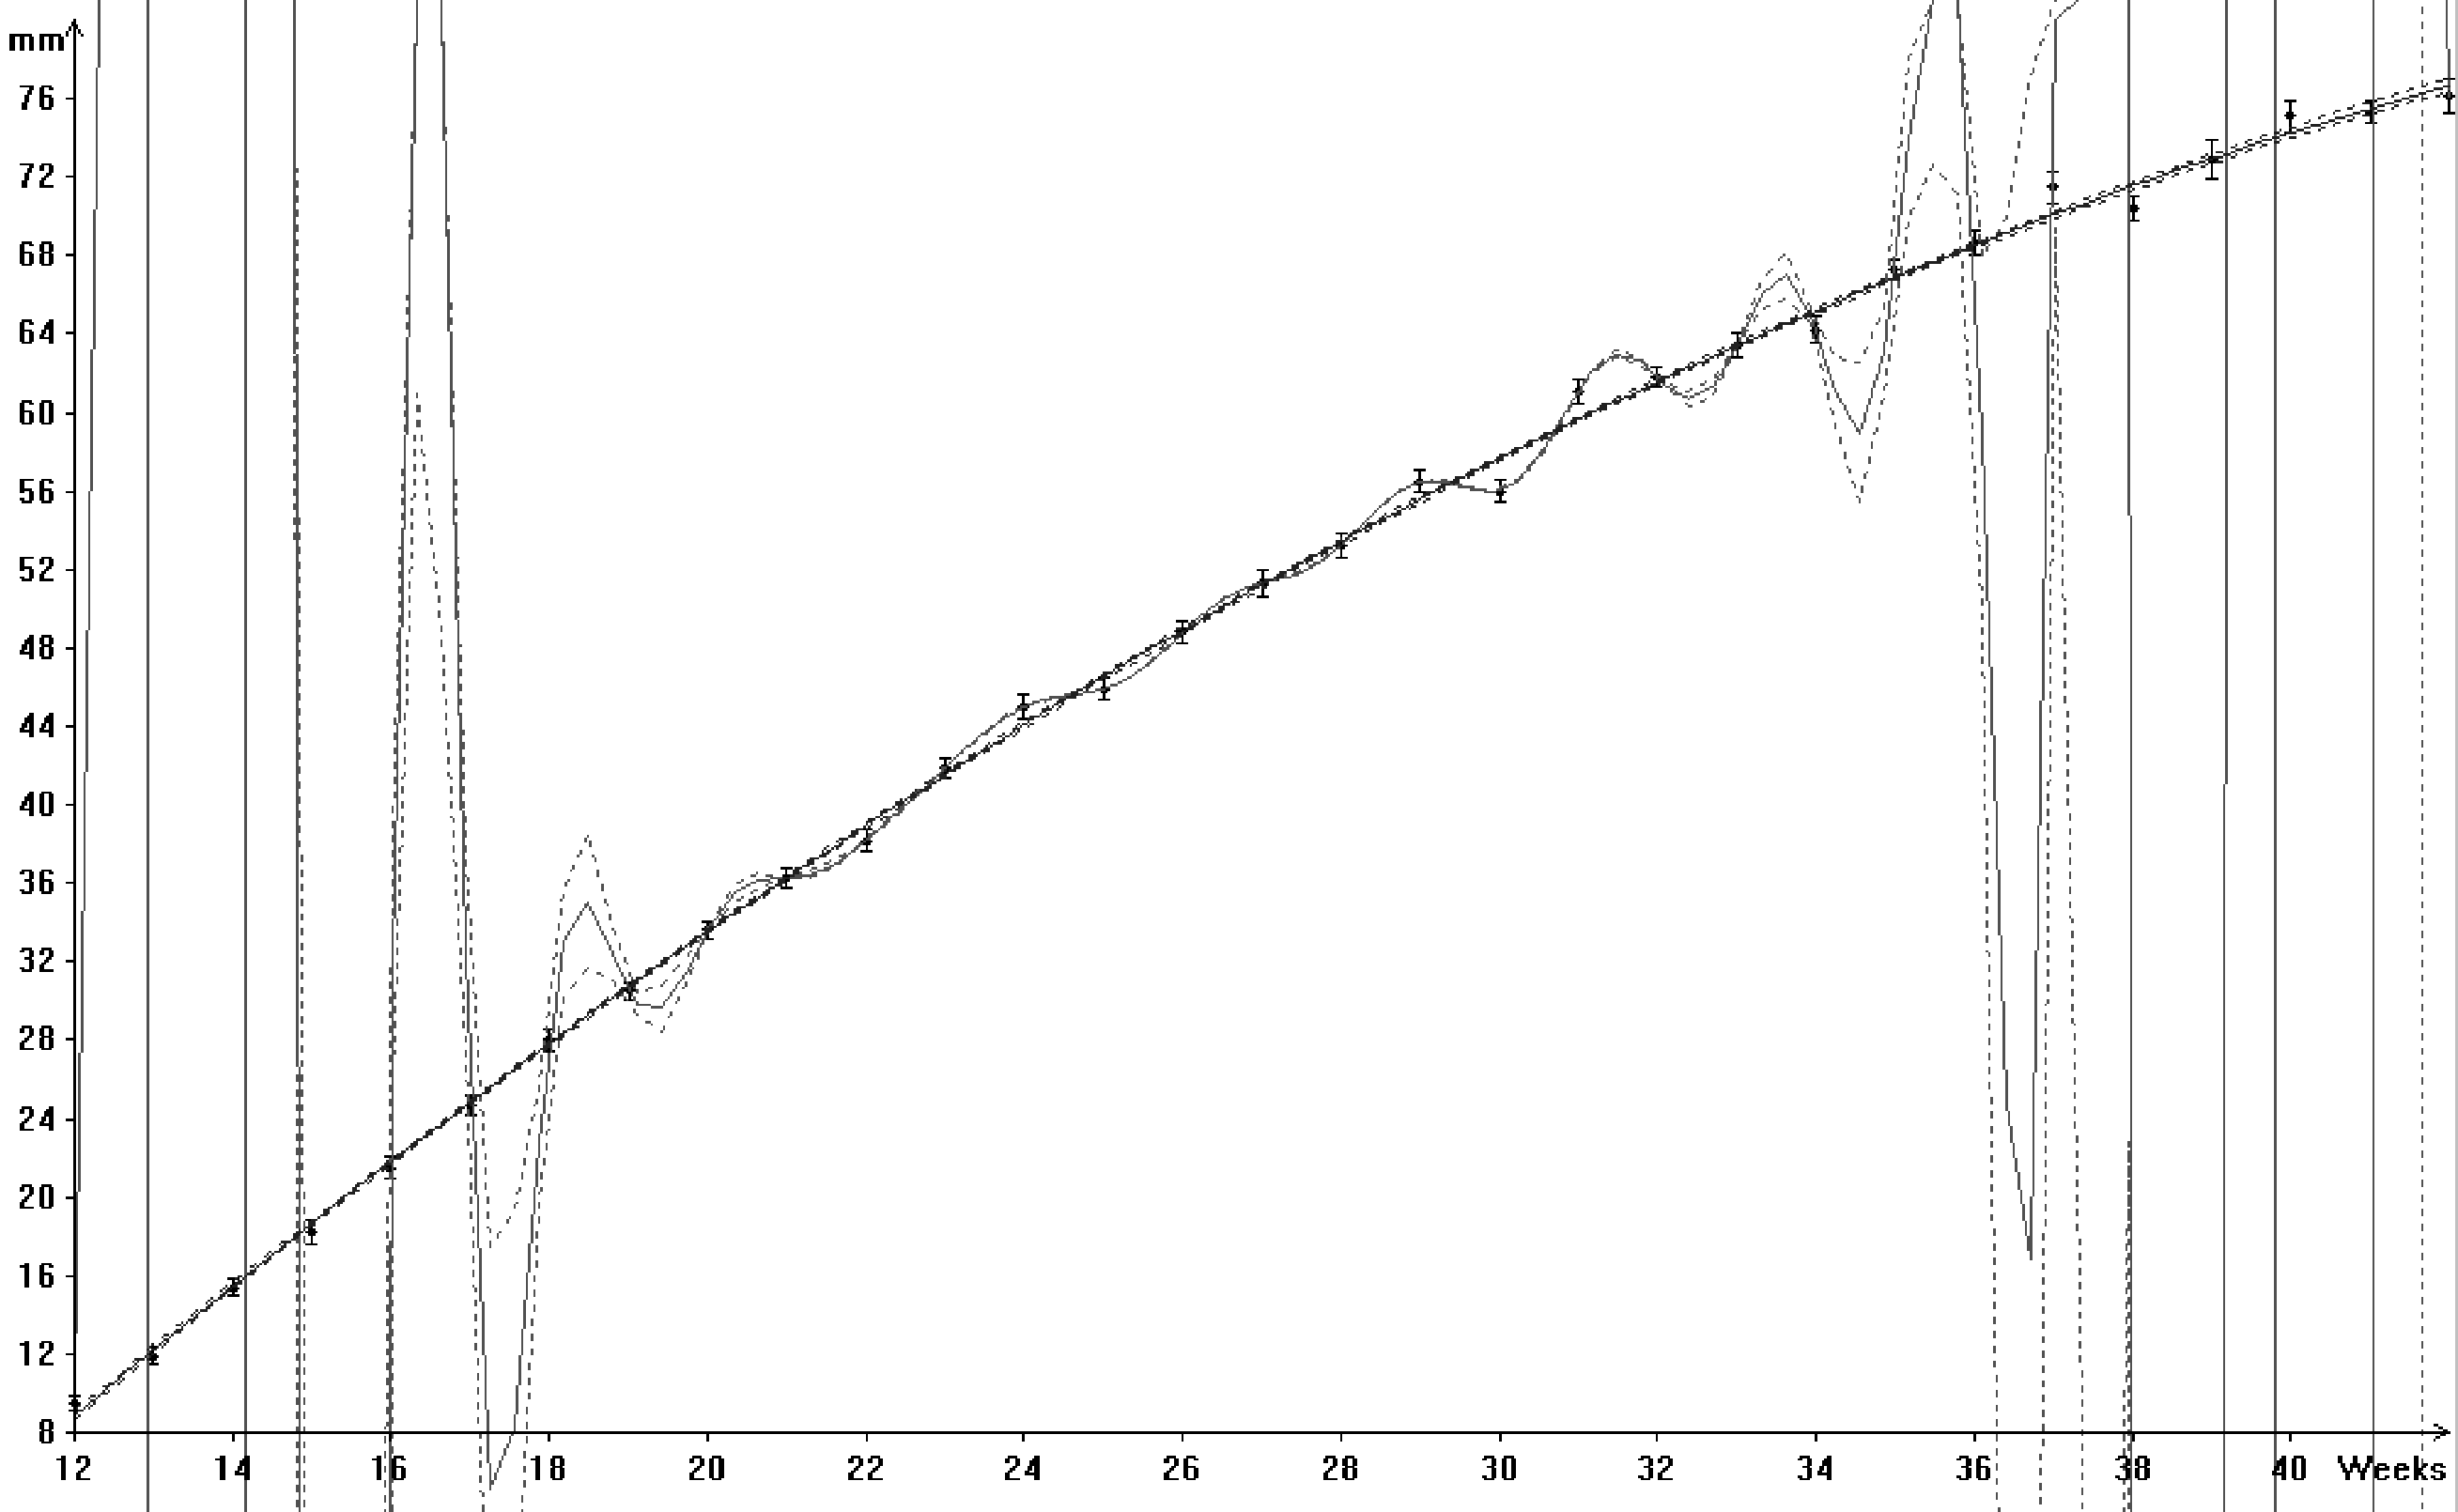
\includegraphics[width=12cm]{Figures/FemurLength}
\caption{Example of polynomial fit} \label{fig:femurLength}
\end{figure}
Each measurement has been obtained by measuring the length of
different fetuses at the same gestational age. The measurement are
averaged and the error on the average is also calculated (\cf
section \ref{sec:moments}).

The obtained data do not follow a smooth curve since the data have
been determined experimentally. The exact date of conception
cannot be exactly determined so some fluctuation is expected, but
the major limitation of the data is to obtain an sufficient number
of measurements to smooth out the natural variations between
individuals. The data from figure \ref{fig:femurLength} have been
fitted with a second order polynomial: the result is shown with a
black thin curve. As one can see, the fit is excellent in spite of
the fluctuation of the measurements. Figure
\ref{fig:femurLengthResults} shows the fit results. This $\chi^2$
confidence level is rather good.
\begin{figure}[h]
\centering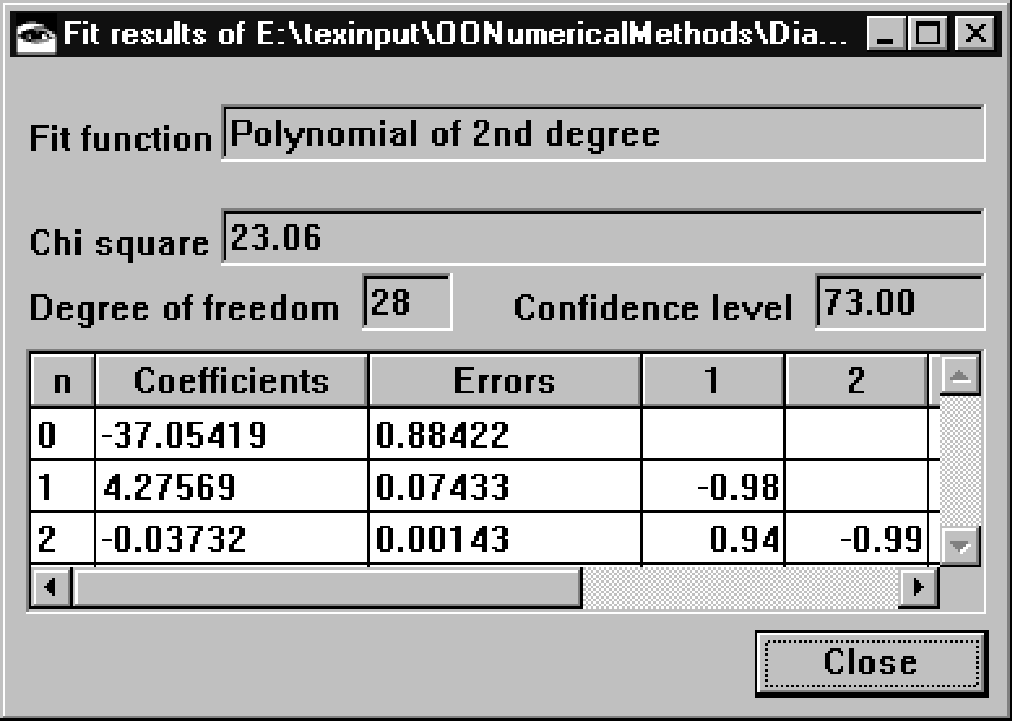
\includegraphics[width=8cm]{Figures/PolFitResults}
\caption{Fit results for the fit of figure \ref{fig:femurLength}
}\label{fig:femurLengthResults}
\end{figure}
However, the correlation coefficients are quite high. This is
usually the case with polynomial fits as each coefficient strongly
depends on the other.

The thick gray line on figure \ref{fig:femurLength} shows the
interpolation polynomial\footnote{An attentive reader will notice
that the interpolation curve dos not go through some data points.
This is an artifact of the plotting over a finite sample of points
which do not coincide with the measured data.} for comparison
(interpolation is discussed in chapter \ref{ch:interpolation}). As
the reader can see the interpolation polynomial gives unrealistic
results because of the fluctuations of the experimental data.

Polynomial fits have something in common with interpolation: a
fitted polynomial can seldom be used to extrapolate the data
outside of the interval defined by the reference points. This is
illustrated on figure \ref{fig:polFitLimit} showing a second order
polynomial fit made on a series of points. This series is
discussed in section \ref{sec:interpolgen} (figure
\ref{fig:interpolex4}).
\begin{figure}
\centering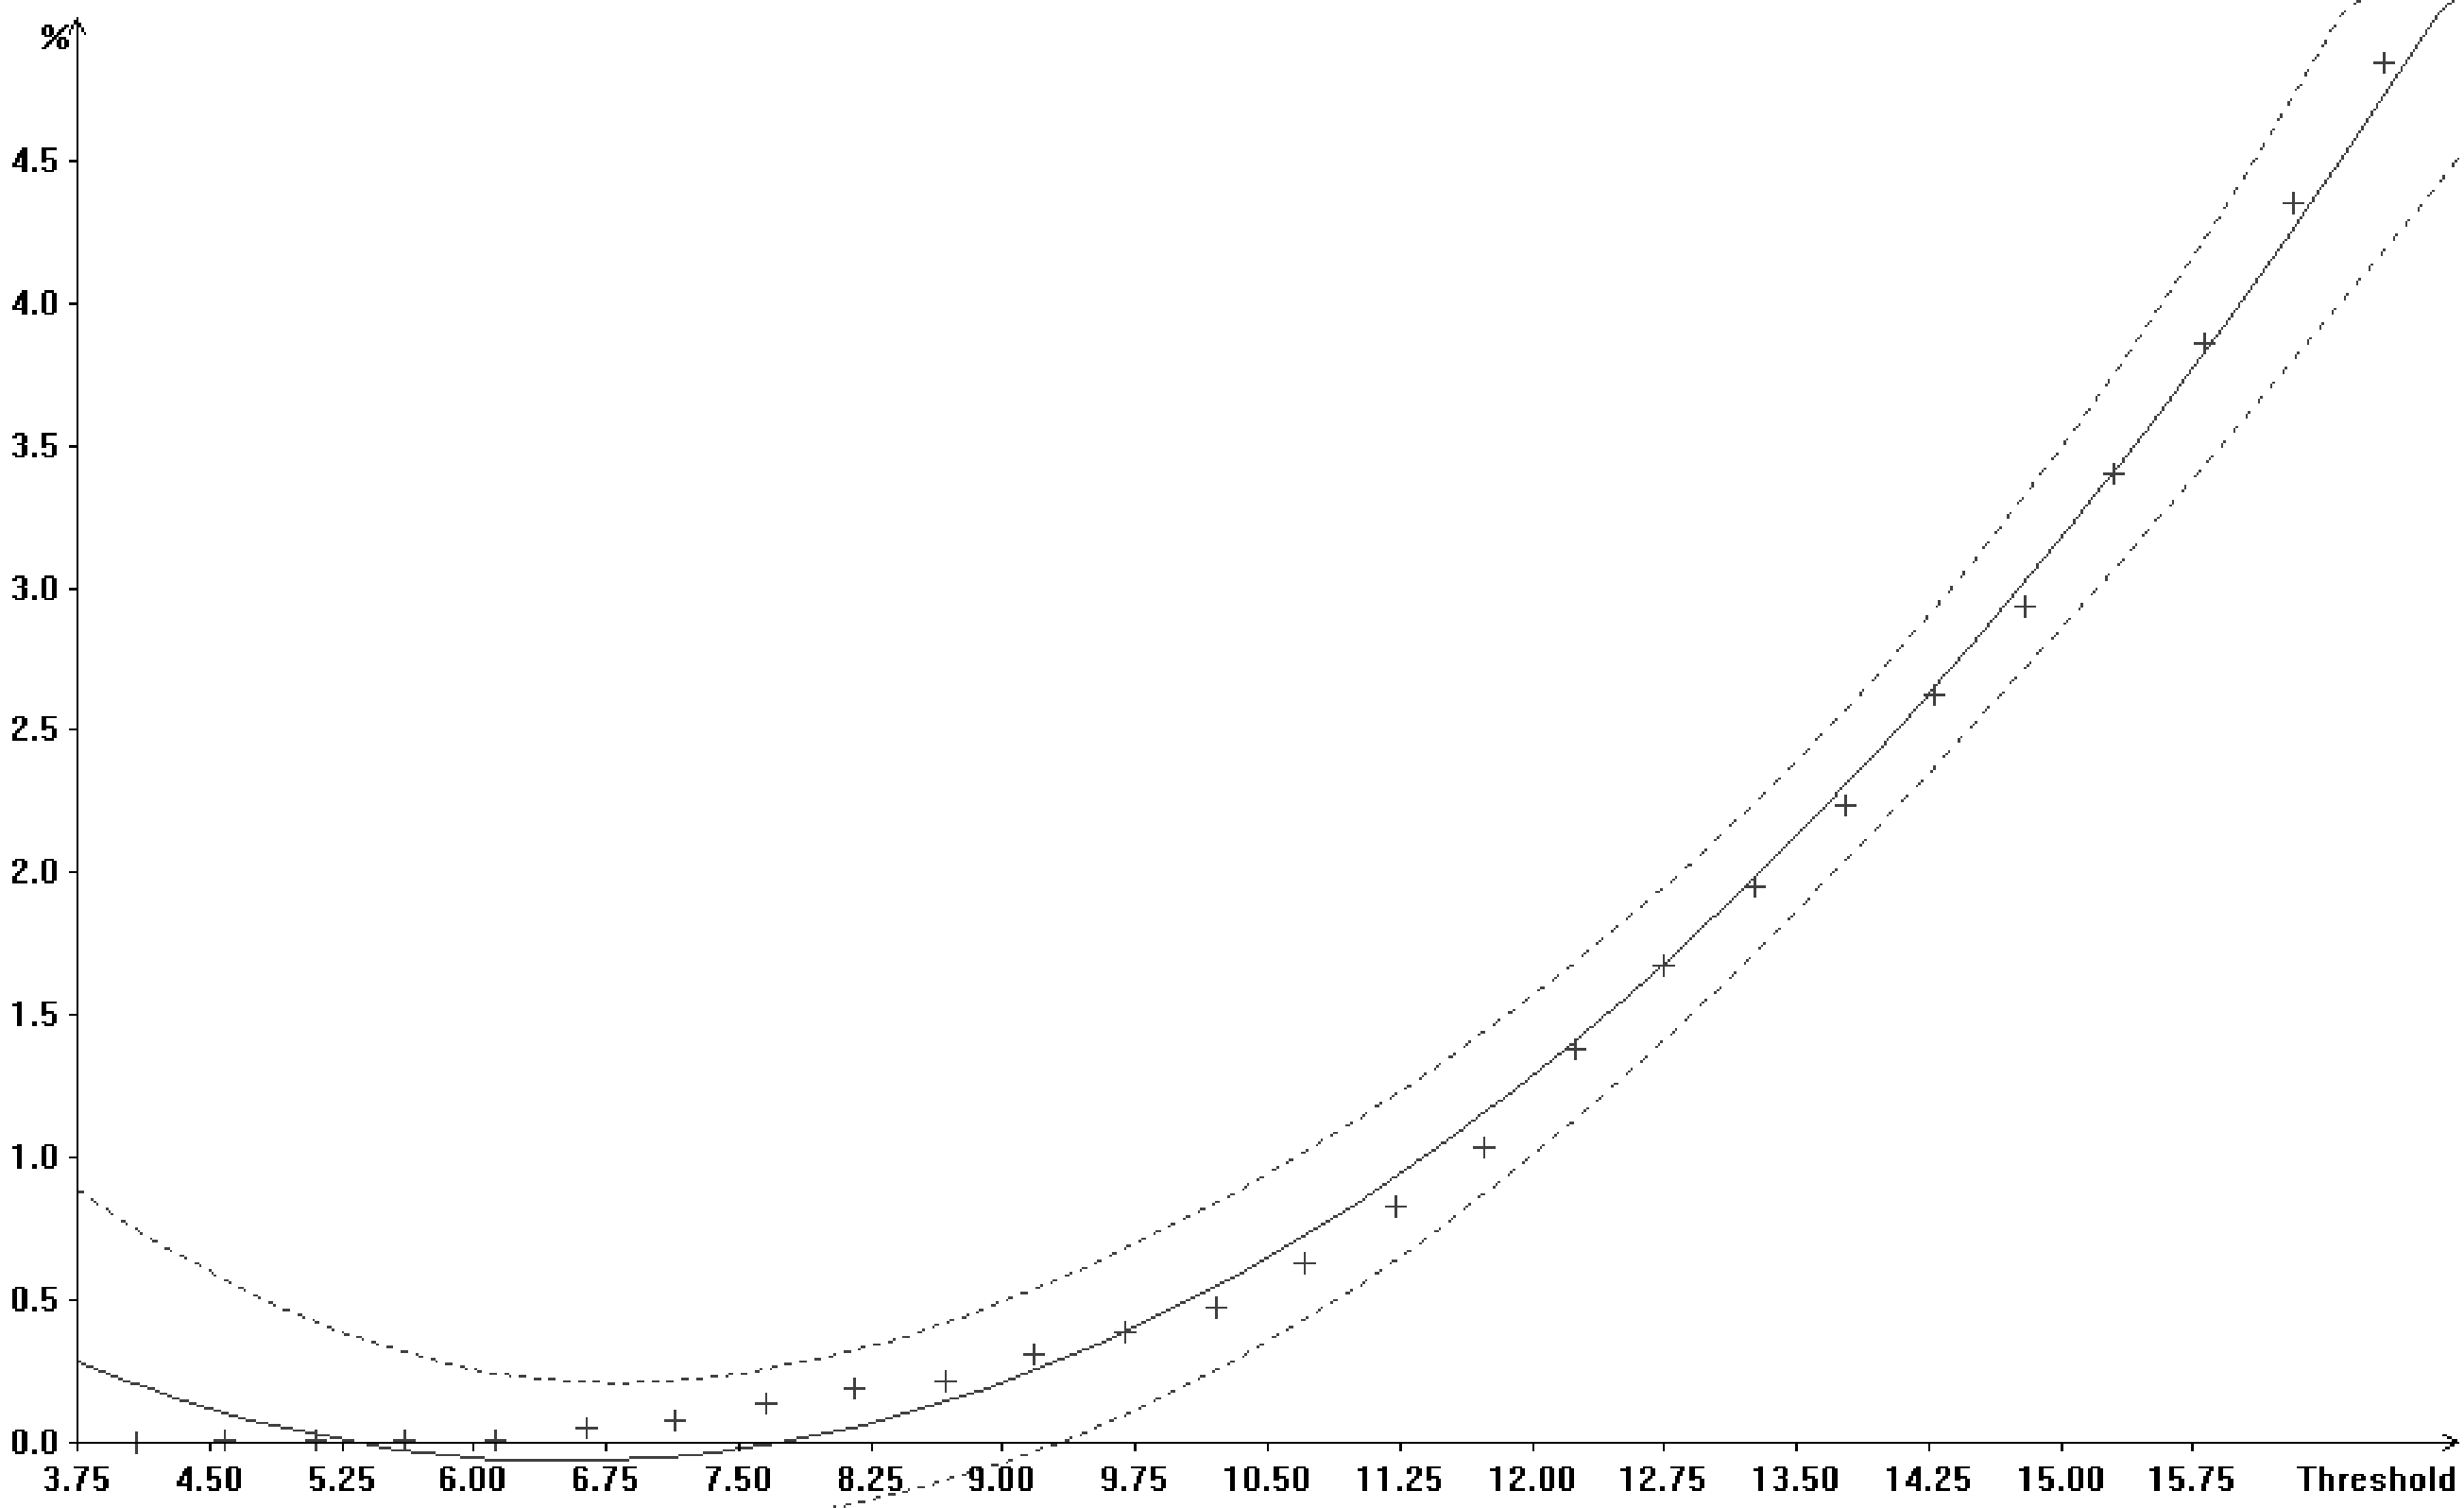
\includegraphics[width=12cm]{Figures/PolFitLimit}
\caption{Limitation of polynomial fits}\label{fig:polFitLimit}
\end{figure}
The reader can see that the fitted polynomial does not reproduce
the behavior of the data in the lower part of the region.
Nevertheless, the data are well within the estimated error. Thus,
the fit results are consistent. Unfortunately too many fit results
are presented without their estimated error. This kind of
information, however, is an essential part of a fit and should
always be deliver along with the fitted function.

This is the idea behind what we call estimated polynomials. An
estimated polynomial is a polynomial whose coefficients have been
determined by a least square fit. An estimated polynomial keeps
the error matrix of the fit is along with the coefficients of the
fitted polynomial.

\subsection{Polynomial least square fits --- Smalltalk  implementation}
\marginpar{Figure \ref{fig:estimationclasses} with the boxes {\textbf
PolynomialLeastSquareFit} and {\textbf EstimatedPolynomial} grayed.}
\label{sec:slsfpol} Listing \ref{ls:lspolynom} shows the complete
implementation in Smalltalk. The following code example show how
to perform the fit made in figure \ref{fig:femurLength}.
\begin{displaycode}{Smalltalk}
 | fit valueStream dataHolder estimation value error|
\end{displaycode}
 \hfil {\texttt<\textsl Accumulation of data into \texttt dataHolder>}
\begin{displaycode}{Smalltalk}
 fit := PMPolynomialLeastSquareFit new: 2.
 dataHolder pointsAndErrorsDo: [ :each | fit add: each].
 estimation := fit evaluate.
 value := estimation value: 20.5.
 error := estimation error: 20.5.
\end{displaycode}

The data are accumulated into a object called {\texttt dataHolder}
implementing the iterator method {\texttt pointsAndErrorsDo}. The
argument of the block used by this method is an instance of class
{\texttt PMWeightedPoint} described in section
\ref{sec:weightedPoint}. The iterator method acts on all
experimental data stored in {\texttt dataHolder}. Next, an instance of
class {\texttt PMPolynomialLeastSquareFit} is created. The argument
of the method is the degree of the polynomial; here a second order
polynomial is used. After data have been accumulated into this
object, the fit is performed by sending the method {\texttt evaluate}
to the fit object. This method returns a polynomial including the
error matrix. The last three lines compute the predicted femur
length and its error in the middle of the $20\th$ week of
pregnancy.

The Smalltalk implementation assumes the points are stored in an
object implementing the iterator method {\texttt do:}.
Any instance of
{\texttt Collection} of its subclasses will work. Each element of the
collection must be an array containing the values $x_i$, $y_i$ and
$1/\sigma_i$.
The class {\texttt PMPolynomialLeastSquareFit} keeps
this collection in the instance variable {\texttt pointCollection}. A
second instance variable, {\texttt degreePlusOne}, keeps the number of
coefficients to be estimated by the fit.

The class creation method {\texttt new:} is used to create an instance
by supplying the degree of the fit polynomial as argument. {\texttt
pointCollection} is set to a new instance of an {\texttt
OrderedCollection}. Then, new values can be added to the fit
instance with the method {\texttt add:}.

The other class creation method, {\texttt new:on:} takes two
arguments: the degree of the fit polynomial and the collection of
points. The fit result can be fetched directly after the creation.

The method {\texttt evaluate} solves equation \ref{eq:lsequs} by first
computing the inverse of the matrix ${\textbf M}$ to get the error
matrix. The coefficients are then obtained from the multiplication
of the constant vector by the error matrix.
\begin{listing} Smalltalk implementation of a polynomial least square fit \label{ls:lspolynom}
$$\halign{ #\hfil&\quad#\hfil\cr {\sl Class}& {\Large\bf DhbPolynomialLeastSquareFit}\cr
{\sl Subclass of }&{\tt Object}\cr\noalign{\vskip 1ex}

{\sl Instance variable names:}&\parbox[t]{4 in}{\tt  pointCollection degreePlusOne }\cr\noalign{\vskip 1ex}}$$


Class methods
{\parskip 1ex\par\noindent}
{\bf new:} {\tt anInteger}
\begin{verbatim}
    ^ super new initialize: anInteger
\end{verbatim}
{\bf new:} {\tt anInteger} {\bf on:} {\tt aCollectionOfPoints}
\begin{verbatim}
    ^ super new initialize: anInteger on: aCollectionOfPoints
\end{verbatim}

Instance methods
{\parskip 1ex\par\noindent}
{\bf accumulate:} {\tt aWeightedPoint} {\bf into:} {\tt aVectorOfVectors} {\bf and:} {\tt aVector}
\begin{verbatim}
OfVectors and: aVector
    | t p powers |
    p := 1.0.
    powers := aVector collect: [ :each | t := p. p := p * 
                                            aWeightedPoint xValue. t].
    aVector accumulate: powers * (aWeightedPoint yValue * 
                                               aWeightedPoint weight).
    1 to: aVector size do:
        [ :k |
          (aVectorOfVectors at: k) accumulate: powers * ((powers 
                                      at: k) * aWeightedPoint weight).
        ].
\end{verbatim}
{\bf add:} {\tt aWeightedPoint}
\begin{verbatim}
    ^ pointCollection add: aWeightedPoint
\end{verbatim}
{\bf computeEquations}
\begin{verbatim}
    | rows vector |
    vector := ( DhbVector new: degreePlusOne) atAllPut: 0 ; yourself.
    rows := ( 1 to: degreePlusOne) collect: [ :k | ( DhbVector new: 
                               degreePlusOne) atAllPut: 0 ; yourself].
    pointCollection do:
        [ :each | self accumulate: each into: rows and: vector].
    ^ Array with: ( DhbSymmetricMatrix rows: rows) with: vector
\end{verbatim}
{\bf evaluate}
\begin{verbatim}
    | system errorMatrix |
    system := self computeEquations.
    errorMatrix := ( system at: 1) inverse.
    ^ (DhbEstimatedPolynomial coefficients: errorMatrix * (system at: 
                                                                   2))
            errorMatrix: errorMatrix;
            yourself
\end{verbatim}
{\bf initialize:} {\tt anInteger}
\begin{verbatim}
    ^ self initialize: anInteger on: OrderedCollection new
\end{verbatim}
{\bf initialize:} {\tt anInteger} {\bf on:} {\tt aCollectionOfPoints}
\begin{verbatim}
    pointCollection := aCollectionOfPoints.
    degreePlusOne := anInteger + 1.
    ^ self
\end{verbatim}


\end{listing}

Listing \ref{ls:estpolynom} show the implementation of the class
{\texttt PMEstimatedPolynomial} which is a subclass of the class {\texttt PMPolynomial} containing the error matrix of the fit performed to
make a estimation of the polynomial's coefficients. The method
{\texttt error:} returns the estimated error of its value based on the
error matrix of the fit using equation \ref{eq:fitError}. The
convenience method {\texttt valueAndError:} returns an array
containing the estimated value and its error in single method
call. This is suitable for plotting the resulting curve.

\begin{listing} Smalltalk implementation of a polynomial with error \label{ls:estpolynom}
$$\halign{ #\hfil&\quad#\hfil\cr {\sl Class}& {\Large\bf DhbEstimatedPolynomial}\cr
{\sl Subclass of }&{\tt DhbPolynomial}\cr\noalign{\vskip 1ex}

{\sl Instance variable names:}&\parbox[t]{4 in}{\tt  errorMatrix }\cr\noalign{\vskip 1ex}}$$


Instance methods
{\parskip 1ex\par\noindent}
{\bf error:} {\tt aNumber}
\begin{verbatim}
    | errorVector term nextTerm |
    nextTerm := 1.
    errorVector := (coefficients collect: [ :each | term := 
            nextTerm. nextTerm := aNumber * nextTerm. term]) asVector.
    ^ (errorVector * errorMatrix * errorVector) sqrt
\end{verbatim}
{\bf errorMatrix}
\begin{verbatim}
    ^ errorMatrix
\end{verbatim}
{\bf errorMatrix:} {\tt aMatrix}
\begin{verbatim}
    errorMatrix := aMatrix.
\end{verbatim}
{\bf valueAndError:} {\tt aNumber}
\begin{verbatim}
    ^ Array with: ( self value: aNumber) with: ( self error: aNumber)
\end{verbatim}


\end{listing}


\section{Least square fit with non-linear dependence}
\label{sec:lsfnonlin} In the case of a non-linear function, the
fit can be reduced to a linear fit and a search by successive
approximations.

Let us assume that we have an approximate estimation ${\textbf p}_0$
of the parameters ${\textbf p}$. Let us define the vector $\Delta{\textbf
p}={\textbf p}-{\textbf p}_0$. One redefines the function $F\left({\textbf
x},{\textbf p}\right)$ as:
\begin{equation}
\label{eq:linexpans}
  F\left({\textbf x},{\textbf p}\right)=F\left({\textbf x},{\textbf p}_0\right)
  +\left.{\displaystyle\partial F\left({\textbf x},{\textbf
  p}\right)\over\displaystyle\partial{\textbf p}}\right|_{{\textbf p}={\textbf
  p}_0}\cdot \Delta{\textbf p}.
\end{equation}
Equation \ref{eq:linexpans} is a linear expansion\footnote{That
is, the first couples of terms of a Taylor expansion of the
function $F\left({\textbf x},{\textbf p}\right)$ around the vector ${\textbf
p}_0$ in an $m$ dimensional space.} of the function $F\left({\textbf
x},{\textbf p}\right)$ around the vector ${\textbf p}_0$ respective to the
vector ${\textbf p}$.
In equation \ref{eq:linexpans}
$\left.{\displaystyle\partial F\left({\textbf x},{\textbf
p}\right)\over\displaystyle\partial{\textbf p}}\right|_{{\textbf p}={\textbf
p}_0}$ is the gradient of the function $F\left({\textbf x},{\textbf
p}\right)$relative to the vector ${\textbf p}$ evaluated for ${\textbf
p}={\textbf p}_0$; this is a vector with the same dimension as the
vector ${\textbf p}$.
Then, one minimizes the expression in equation
\ref{eq:lsestim} respective to the vector $\Delta{\textbf p}$. This is
of course a linear problem as described in section
\ref{eq:lslinear}. Equation \ref{eq:lsmequs} becomes:
\begin{equation}
\label{eq:lslinequs}
  {\textbf M}\cdot\Delta{\textbf p}={\textbf c},
\end{equation}
where the components of the matrix ${\textbf M}$ are now defined by:
\begin{equation}
\label{eq:lsmatrix}
  M_{jk}=\sum_{i=1}^N {\displaystyle
  1\over\displaystyle\sigma_i^2}\cdot\left.{\displaystyle\partial F\left({\textbf x}_i,{\textbf
p}\right)\over\displaystyle\partial p_j}\right|_{{\textbf p}={\textbf
p}_0}\cdot\left.{\displaystyle\partial F\left({\textbf x}_i,{\textbf
p}\right)\over\displaystyle\partial p_k}\right|_{{\textbf p}={\textbf
p}_0}
\end{equation}
and the components of the vector ${\textbf c}$ are defined by:
\begin{equation}
\label{eq:lsvector}
  c_j=\sum_{i=1}^N {\displaystyle
  y_i-F\left({\textbf x}_i,{\textbf
p}_0\right)\over\displaystyle\sigma_i^2}\cdot\left.{\displaystyle\partial
F\left({\textbf x}_i,{\textbf p}\right)\over\displaystyle\partial
p_j}\right|_{{\textbf p}={\textbf p}_0}.
\end{equation}
The vector $\Delta{\textbf p}$ is obtained by solving equation
\ref{eq:lslinequs} using the algorithms described in sections
\ref{sec:lineqs} and \ref{sec:lup}. Then, we can use the vector
${\textbf p}_0+\Delta{\textbf p}$ as the new estimate and repeat the whole
process. One can show\footnote{A mathematically oriented reader
can see that this is a generalization of the Newton zero-finding
algorithm (\cf section \ref{sec:newton})to $m$ dimensions .} that
iterating this process converges toward the vector $\bar{\textbf p}$
minimizing the function $S\left({\textbf p}\right)$ introduced in
equation \ref{eq:lsestim}.

As explained in section \ref{eq:lslinear}, the inverse of the
matrix ${\textbf M}$ is the error matrix containing the variance of
each parameter and their correlation. The expression for the
estimated variance on the function $F\left({\textbf x},{\textbf p}\right)$
becomes:
\begin{equation}
\label{eq:nllserror}
  \var\left[F\left({\textbf x},{\textbf p}\right)\right]=
  \sum_{j=1}^m\sum_{k=1}^m M_{jk}^{-1}\cdot
  {\displaystyle\partial F\left({\textbf x}_i,\bar{\textbf
p}\right)\over\displaystyle\partial
p_j}\cdot{\displaystyle\partial F\left({\textbf x}_i,\bar{\textbf
p}\right)\over\displaystyle\partial p_k}.
\end{equation}
A careful examination of the error matrix can tell whether or not
the fit is meaningful.

Figure \ref{fig:lsfExample} shows an example of a least square fit
performed on a histogram with a probability density function.
\begin{figure}
\centering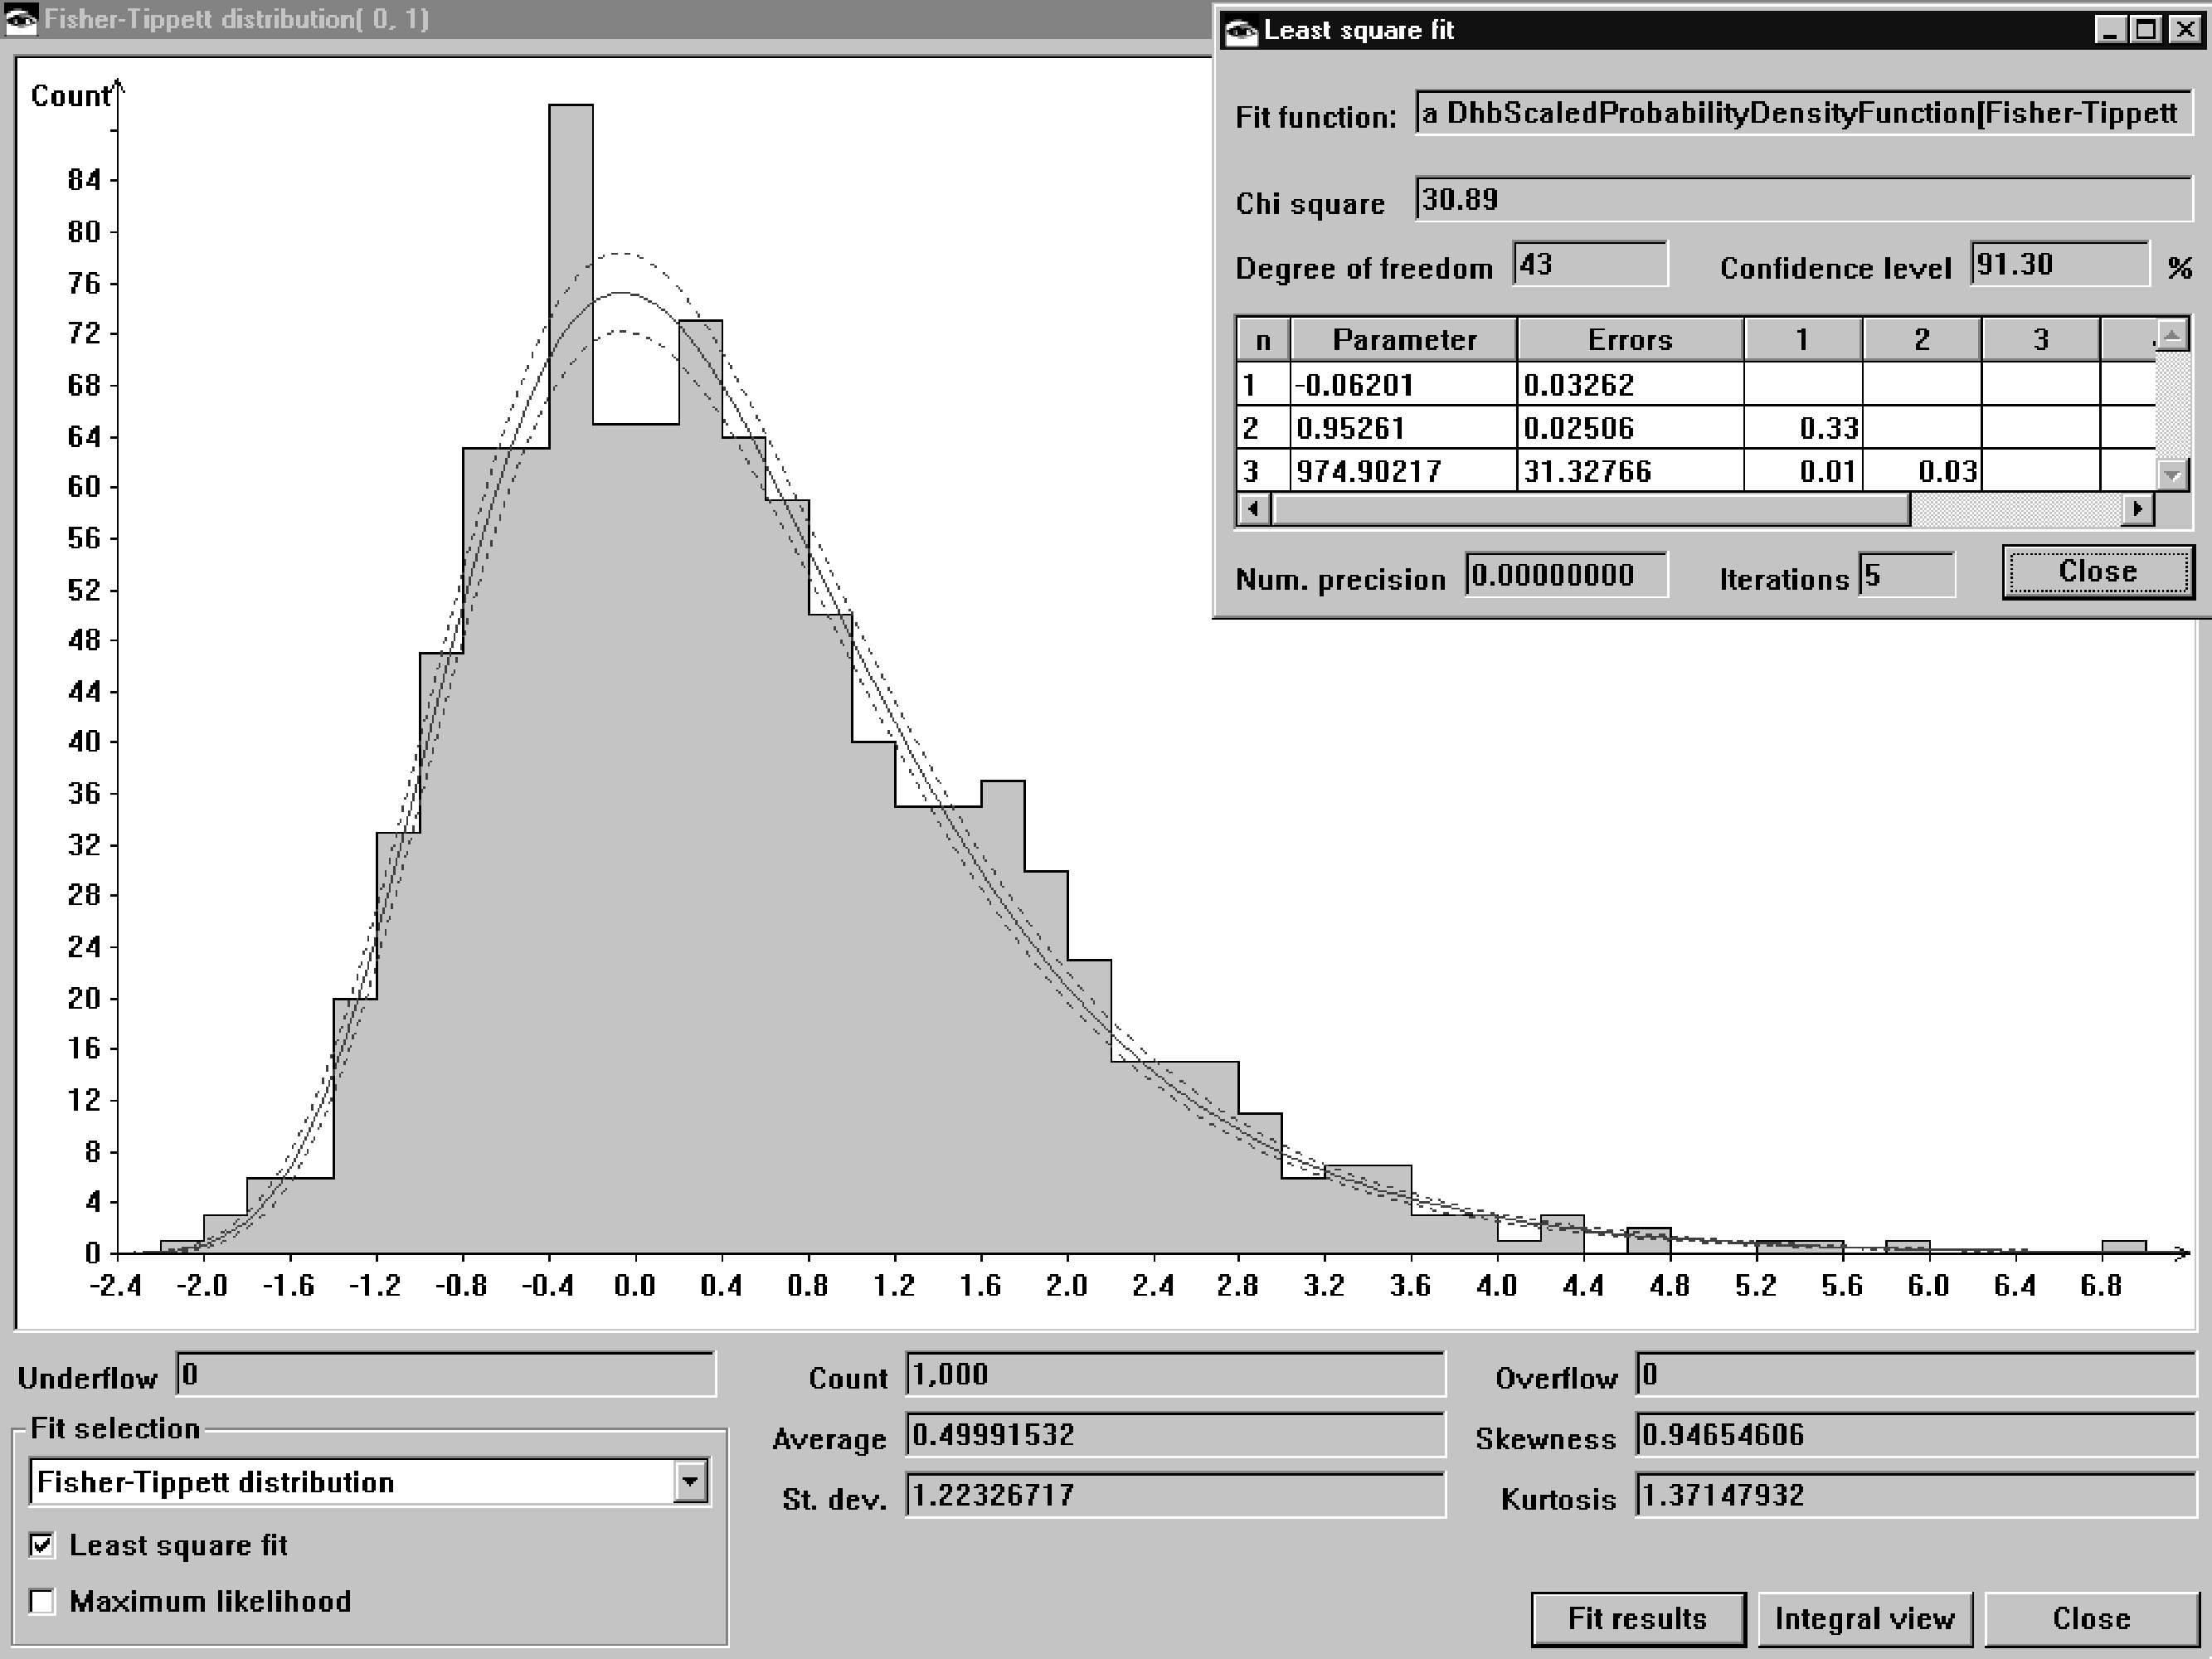
\includegraphics[width=11cm]{Figures/LeastSquareFit}
\caption{Example of a least square fit}\label{fig:lsfExample}
\end{figure}
The histogram of figure \ref{fig:lsfExample} was generated using a
random generator distributed according to a Fisher-Tippett
distribution (\cf \ref{sec:fishertippettdist}) with parameters
$\alpha = 0$ and $\beta=1$. Only 1000 events have been accumulated
into the histogram. The inset window in the upper right corner
shows the fit results. The order of the parameter are $\alpha$,
$\beta$ and the number of generated events. The solid curve laid
onto the histogram is the prediction of the fitted function; the
two dotted lines indicate the error on the prediction. The reader
can verify that the fit is excellent. The number of needed
iterations is quite low: the convergence of the algorithm is quite
good in general.

\subsection{Non-linear fit --- General implementation}
\marginpar{Figure \ref{fig:estimationclasses} with the box {\textbf
LeastSquareFit} grayed.} As we have seen the solution of a
non-linear fit can be approximated by successive approximations.
Thus, non-linear fits are implemented with a subclass of the
iterative process class described in section \ref{sec:iteration}.
Data points must be kept in a structure maintained by the object
implementing linear least square fit to be readily available at
each iteration. Thus, the data point are kept in an instance
variable.

The result of the iterative process are the parameters. Our
implementation assumes that the supplied function contains and
maintains its parameter. Thus, the instance variable corresponding
to the result of the iterative process is the fit function itself.
The parameters determined by the fit --- the result proper --- are
kept within the object implementing the supplied function. In
particular the determination of the initial values for the
iterative process are the responsibility of the fit function.
Thus, the method {\texttt initializeIterations} does not do anything.

In most cases, the number of parameters in a least square fits is
relatively small. Thus, LUP decomposition --- described in section
\ref{sec:lup} --- is sufficient to solve equation
\ref{eq:lslinequs} at each iteration. Except for the last
iteration, there is no need to compute the error matrix (the
inverse of the matrix ${\textbf M}$. The components of the error
matrix can be obtained from the LUP decomposition when the
algorithm converges.

Convergence is attained when the largest of the relative variation
of the components of the vector becomes smaller than a given
value. In addition to the fact that we are dealing with floating
point numbers, the reason for using relative precision is that the
components of the vector ${\textbf p}$ usually have different ranges.

When the fit has been obetained, convenience methods allows to
retrieve the sum of equation \ref{eq:lsmlestim} ({\texttt chiSquare})
and the confidence level of the fit ({\texttt confidenceLevel}).
Another convenience method, {\texttt valueAndError} computes the
prediction of the fit and its estimated error using equation
\ref{eq:nllserror}.

\subsection{Non-linear fit --- Smalltalk implementation}
\label{sec:slsfnonlin}Listing \ref{ls:lsfnonlin} shows the
complete implementation in Smalltalk. The following code example
shows how the data of figure \ref{fig:lsfExample} were
generated\footnote{$\ldots$up to the plotting facilities. This
could be the topic of a future book.d}.
\begin{displaycode}{Smalltalk}
\label{exs:leastSquare}
 | genDistr hist fit |
 hist := PMHistogram new.
 hist freeExtent: true.
 genDistr := PMFisherTippettDistribution shape: 0 scale: 1.
 1000 timesRepeat: [ hist accumulate: genDistr random ].
 fit := PMLeastSquareFit histogram: hist
            distributionClass: DhbFisherTippettDistribution.
 fit evaluate.
\end{displaycode}
The first two lines after the declaration define an instance of
class {\texttt PMHistogram} with automatic adjustment of the limits
(\cf section \ref{sec:shistogram}).
The next line defines an
instance of a Fisher-Tippett distribution. Then, 1000 random
numbers generated according to this distribution are accumulated
into the histogram. Next, an instance if the class {\texttt
PMLeastSquareFit} is defined with the histogram for the data
points and the desired class of the probability density function.
The corresponding scaled probability is created within the method
(\cf listing \ref{ls:lsfnonlin}). the final line performs the fit
proper. After this line, the calling application can either use
the fit object or extract the fit result to make predictions with
the fitted distribution.

The class {\texttt PMLeastSquareFit} is a subclass of {\texttt
PMIterativeProcess} described in section \ref{sec:siteration}. It
has the following instance variables:
\begin{description}
  \item[\texttt dataHolder] is the object containing the experimental
  data; this object must implement the iterator method {\texttt
  pointsAndErrorsDo:}; the block supplied to the iterator method
  takes as argument an instance of the class {\texttt
  PMWeightedPoint} described in section \ref{sec:weightedPoint};
  \item[\texttt equations] contains the components of the matrix ${\textbf
  M}$;
  \item[\texttt constants] contains the components of the vector ${\textbf
  c}$;
  \item[\texttt errorMatrix] contains the LUP decomposition of the matrix ${\textbf
  M}$;
  \item[\texttt chiSquare] contains the sum of equation \ref{eq:lsmlestim};
  \item[\texttt degreeOfFreedom] contains the degree of freedom of the
  fit.
\end{description}
The instance variables {\texttt errorMatrix}, {\texttt chiSquare} and {\texttt
degreeOfFreedom} are implemented using lazy initialization. The
method {\texttt finalizeIterations} sets the instance variables {\texttt
equations} and {\texttt constants} to {\texttt nil} to reclaim space at
the end of the fit.

The supplied fit function --- instance variable {\texttt result} ---
must implement the method {\texttt valueAndGradient:} which returns an
array containing the value of the function at the supplied
argument and the gradient vector. This is an optimization because
the gradient can be computed frequently using intermediate results
coming from the computation of the function's value.

The method {\texttt valueAndError:} is a good example of using the
vector and matrix operations described in chapter
\ref{ch:linearalgebra}.

\begin{listing} Smalltalk implementation of a non-linear
least square fit \label{ls:lsfnonlin}
$$\halign{ #\hfil&\quad#\hfil\cr {\sl Class}& {\Large\bf DhbLeastSquareFit}\cr
{\sl Subclass of }&{\tt DhbIterativeProcess}\cr\noalign{\vskip 1ex}

{\sl Instance variable names:}&\parbox[t]{4 in}{\tt  dataHolder errorMatrix chiSquare equations constants degreeOfFreedom }\cr\noalign{\vskip 1ex}}$$


Class methods
{\parskip 1ex\par\noindent}
{\bf histogram:} {\tt aHistogram} {\bf distributionClass:} {\tt aProbabilityDensityFunctionClass}
\begin{verbatim}
    ^ self points: aHistogram
        function: (DhbScaledProbabilityDensityFunction histogram: 
                                                            aHistogram
                distributionClass: aProbabilityDensityFunctionClass)
\end{verbatim}
{\bf points:} {\tt aDataHolder} {\bf function:} {\tt aParametricFunction}
\begin{verbatim}
    ^ aParametricFunction ifNotNil: [ :dp | super new initialize: 
                                                 aDataHolder data: dp]
\end{verbatim}

Instance methods
{\parskip 1ex\par\noindent}
{\bf accumulate:} {\tt aWeightedPoint}
\begin{verbatim}
    | f g |
    f := result valueAndGradient: aWeightedPoint xValue.
    g := f last.
    f := f first.
    constants accumulate: g * ((aWeightedPoint yValue - f) * 
                                               aWeightedPoint weight).
    1 to: g size do:
        [ :k |
          (equations at: k) accumulate: g * ((g at: k) * 
                                               aWeightedPoint weight).
        ].
\end{verbatim}
{\bf accumulateEquationSystem}
\begin{verbatim}
    dataHolder pointsAndErrorsDo: [ :each | self accumulate: each].
\end{verbatim}
{\bf chiSquare}
\begin{verbatim}
    chiSquare isNil
        ifTrue: [ self computeChiSquare].
    ^ chiSquare
\end{verbatim}
{\bf computeChanges}
\begin{verbatim}
    errorMatrix := DhbLUPDecomposition direct: equations.
    ^ errorMatrix solve: constants
\end{verbatim}
{\bf computeChiSquare}
\begin{verbatim}
    chiSquare := 0.
    degreeOfFreedom := self numberOfFreeParameters negated.
    dataHolder pointsAndErrorsDo:
        [ :each |
          chiSquare := ( each chi2Contribution: result) + chiSquare.
          degreeOfFreedom := degreeOfFreedom + 1.
        ].
\end{verbatim}
{\bf computeEquationSystem}
\begin{verbatim}
    constants atAllPut: 0.
    equations do: [ :each | each atAllPut: 0].
    self accumulateEquationSystem.
\end{verbatim}
{\bf confidenceLevel}
\begin{verbatim}
    ^ (DhbChiSquareDistribution degreeOfFreedom: self 
                      degreeOfFreedom) confidenceLevel: self chiSquare
\end{verbatim}
{\bf degreeOfFreedom}
\begin{verbatim}
    degreeOfFreedom isNil
        ifTrue: [ self computeChiSquare].
    ^ degreeOfFreedom
\end{verbatim}
{\bf errorMatrix}
\begin{verbatim}
    ^ DhbSymmetricMatrix rows: errorMatrix inverseMatrixComponents
\end{verbatim}
{\bf evaluateIteration}
\begin{verbatim}
    | changes maxChange |
    self computeEquationSystem.
    changes := self computeChanges.
    result changeParametersBy: changes.
    maxChange := 0.
    result parameters with: changes do: 
        [ :r :d | maxChange := ( d / r) abs max: maxChange].
    ^maxChange
\end{verbatim}
{\bf finalizeIterations}
\begin{verbatim}
    equations := nil.
    constants := nil.
    degreeOfFreedom := nil.
    chiSquare := nil
\end{verbatim}
{\bf fitType}
\begin{verbatim}
    ^'Least square fit'
\end{verbatim}
{\bf initialize:} {\tt aDataHolder} {\bf data:} {\tt aParametricFunction}
\begin{verbatim}
    dataHolder := aDataHolder.
    result := aParametricFunction.
    ^ self
\end{verbatim}
{\bf initializeIterations}
\begin{verbatim}
    | n |
    n := self numberOfParameters.
    constants := (DhbVector new: n)
                atAllPut: 0;
                yourself.
    equations := (1 to: n) collect: 
                    [:k | 
                    (DhbVector new: n)
                        atAllPut: 0;
                        yourself]
\end{verbatim}
{\bf numberOfFreeParameters}
\begin{verbatim}
    ^ self numberOfParameters
\end{verbatim}
{\bf numberOfParameters}
\begin{verbatim}
    ^ result parameters size
\end{verbatim}
{\bf value:} {\tt aNumber}
\begin{verbatim}
    ^ result value: aNumber
\end{verbatim}
{\bf valueAndError:} {\tt aNumber}
\begin{verbatim}
    | valueGradient |
    valueGradient := result valueAndGradient: aNumber.
    ^Array with: valueGradient first
           with: ( valueGradient last * ( self errorMatrix * 
                                             valueGradient last)) sqrt
\end{verbatim}


\end{listing}

\section{Maximum likelihood fit of a probability density function}
\label{sec:mlfhist} In section \ref{sec:histogram} histograms have
been discussed as a way to represent a probability density
function directly from experimental data. In this section we shall
show that the maximum likelihood estimation can easily be applied
to the data gathered in a histogram in order to determine the
parameters of a hypothesized probability density function.

In general the maximum likelihood fit of a probability density
function to a histogram is much faster than the corresponding
least square fit because the number of free parameters is lower,
as we shall see in this section. In addition, the maximum
likelihood estimation is unbiased and is therefore a better
estimation than the least square fit estimation, especially when
the histogram is sparsely populated. Thus, a maximum likelihood
fit is the preferred way of finding the parameters of a
probability density function from experimental data collected in a
histogram.

Let $m$ be the number of bins in the histogram and let $n_i$ be
the content of the $i^{\mathop{\textrm th}}$ bin. Let $P_i\left({\textbf
p}\right)$ the probability of observing a value in the
$i^{\mathop{\textrm th}}$ bin. The likelihood function $L\left({\textbf
p}\right)$ is the probability of observing the particular
histogram. Since the hypothesis of a probability density function
does not constrain the total number of values collected into the
histogram, the total number of collected values can be considered
as constant. As a consequence, a maximum likelihood fit has one
parameter less than a least square fit using the same function.
Since the total number is unconstrained, the probability of
observing the particular histogram is given by a multinomial
probability. Thus, the likelihood function can be written as:
\begin{equation}
\label{eq:mlfhist}
  L\left({\textbf p}\right)=N!\prod_{i=1}^m{\displaystyle P_i\left({\textbf
  p}\right)^{n_i}\over\displaystyle n_i!},
\end{equation}
where $N=\sum_{i=1}^m n_i$ is the total number of values collected
into the histogram. As we have seen in section \ref{sec:mlf},
finding the maximum of $L\left({\textbf p}\right)$ is equivalent of
finding the maximum of the function $I\left({\textbf p}\right)$. Since
$N$ is a constant, we use a renormalized function:
\begin{equation}
\label{eq:mlogfhist} I\left({\textbf p}\right)=\ln {\displaystyle
M\left({\textbf p}\right) \over\displaystyle N!}=\sum_{i=1}^m n_i \ln
P_i\left({\textbf p}\right).
\end{equation}
Finding the maximum of the function $I\left({\textbf p}\right)$ is
equivalent to solving the following system of non-linear
equations:
\begin{equation}
\label{eq:mlfsys} {\displaystyle\partial I\left({\textbf p}\right)
\over\displaystyle\partial{\textbf p}}=\sum_{i=1}^m {\displaystyle n_i
\over\displaystyle P_i\left({\textbf
p}\right)}\cdot{\displaystyle\partial P_i\left({\textbf p}\right)
\over\displaystyle\partial{\textbf p}}=0.
\end{equation}
This system can be solved with a search by successive
approximations, where a system of linear equations must be solved
at each step. The technique used is similar to the one described
in section \ref{sec:lsfnonlin}. In this case, however, it is more
convenient to expand the inverse of the probability density
function around a previous approximation as follows:
\begin{equation}
{\displaystyle 1\over\displaystyle P_i\left({\textbf p}\right)} =
{\displaystyle 1\over\displaystyle P_i\left({\textbf p}_0\right)} -
{\displaystyle 1\over\displaystyle P_i\left({\textbf
p}_0\right)^2}\cdot \left.{\displaystyle\partial P_i\left({\textbf
p}\right) \over\displaystyle\partial{\textbf p}}\right|_{{\textbf p}={\textbf
p}_0}\cdot\Delta{\textbf p}.
\end{equation}
This expansion can only be defined over a range where the
probability density function is not equal to zero. Therefore, this
expansion of the maximum likelihood estimation cannot be used on a
histogram where bins with non-zero count are located on a range
where the probability density function is equal to
zero\footnote{Equation \ref{eq:mlogfhist} shows that the bins over
which the probability density function is zero give no
information.}. Contrary to a least square fit, bins with zero
count do not participate to the estimation.

Now equation \ref{eq:mlfsys} becomes a system of linear equations
of the type:
\begin{equation}
\label{eq:mlflinequs}
  {\textbf M}\cdot\Delta{\textbf p}={\textbf c},
\end{equation}
where the components of the matrix ${\textbf M}$ are now defined by:
\begin{equation}
\label{eq:mlfmatrix}
 M_{jk}=\sum_{i=1}^m {\displaystyle
n_i\over\displaystyle P_i\left({\textbf p}_0\right)^2
}\cdot\left.{\displaystyle\partial P_i\left({\textbf p}_0\right)
\over\displaystyle\partial p_j} \right|_{{\textbf p}={\textbf
p}_0}\cdot\left.{\displaystyle\partial P_i\left({\textbf p}_0\right)
\over\displaystyle\partial p_k} \right|_{{\textbf p}={\textbf p}_0},
\end{equation}
and those of the vector ${\textbf c}$ by:
\begin{equation}
\label{eq:mlfvector}
 c_j=\sum_{i=1}^m {\displaystyle
n_i\over\displaystyle P_i\left({\textbf p}_0\right)
}\cdot\left.{\displaystyle\partial P_i\left({\textbf p}_0\right)
\over\displaystyle\partial p_j} \right|_{{\textbf p}={\textbf p}_0}.
\end{equation}

As discussed at the beginning of this section, the maximum
likelihood estimation for a histogram cannot determine the total
count in the histogram. The estimated total count, $\bar{N}$, is
estimated with the following hypothesis:
\begin{equation}
   n_i=\bar{N}P\left(\bar{\textbf p}\right),
\end{equation}
where $\bar{\textbf p}$ is the maximum likelihood estimation of the
distribution parameters. The estimation is performed using
$\bar{N}$ as the only variable. The maximum likelihood estimation
cannot be solved analytically, however, the least square
estimation can.

As we have seen in section \ref{sec:chitesthist} the variance of
the bin count is the estimated bin content. Thus, the function to
minimize becomes:
\begin{equation}
\label{eq:mlfnorm}
S\left(\bar{N}\right)=\sum_{i=1}^m{\displaystyle\left[n_i-\bar{N}
P_i\left(\bar{\textbf p}\right)\right]^2
\over\displaystyle\bar{N}P_i\left(\bar{\textbf p}\right)}
\end{equation}
The value of $\bar{N}$ minimizing the expression of equation
\ref{eq:mlfnorm} is:
\begin{equation}
\label{eq:mlfnormsol}
\bar{N}=\sqrt{{\displaystyle\sum_{i=1}^m
n_i^2 / P_i\left(\bar{\textbf p}\right) \over\displaystyle\sum_{i=1}^m
P_i\left(\bar{\textbf p}\right)}}.
\end{equation}
and the estimated error on $\bar{N}$ is given by
\begin{equation}
\label{eq:mlfnormsigma}
\sigma_{\bar{N}}=\sqrt{{\displaystyle\sum_{i=1}^m n_i^2 /
P_i\left(\bar{\textbf p}\right) \over\displaystyle 2 \bar{N}}}.
\end{equation}

After computing $\bar{N}$ using equation \ref{eq:mlfnormsol}, the
goodness of the maximum likelihood fit can be estimated by
calculating the $\chi^2$ confidence level of
$S\left(\bar{N}\right)$ given by equation \ref{eq:mlfnorm}.

Figure \ref{fig:mlfExample} shows an example of a maximum
likelihood fit performed on the same histogram as in figure
\ref{fig:lsfExample}.
\begin{figure}
\centering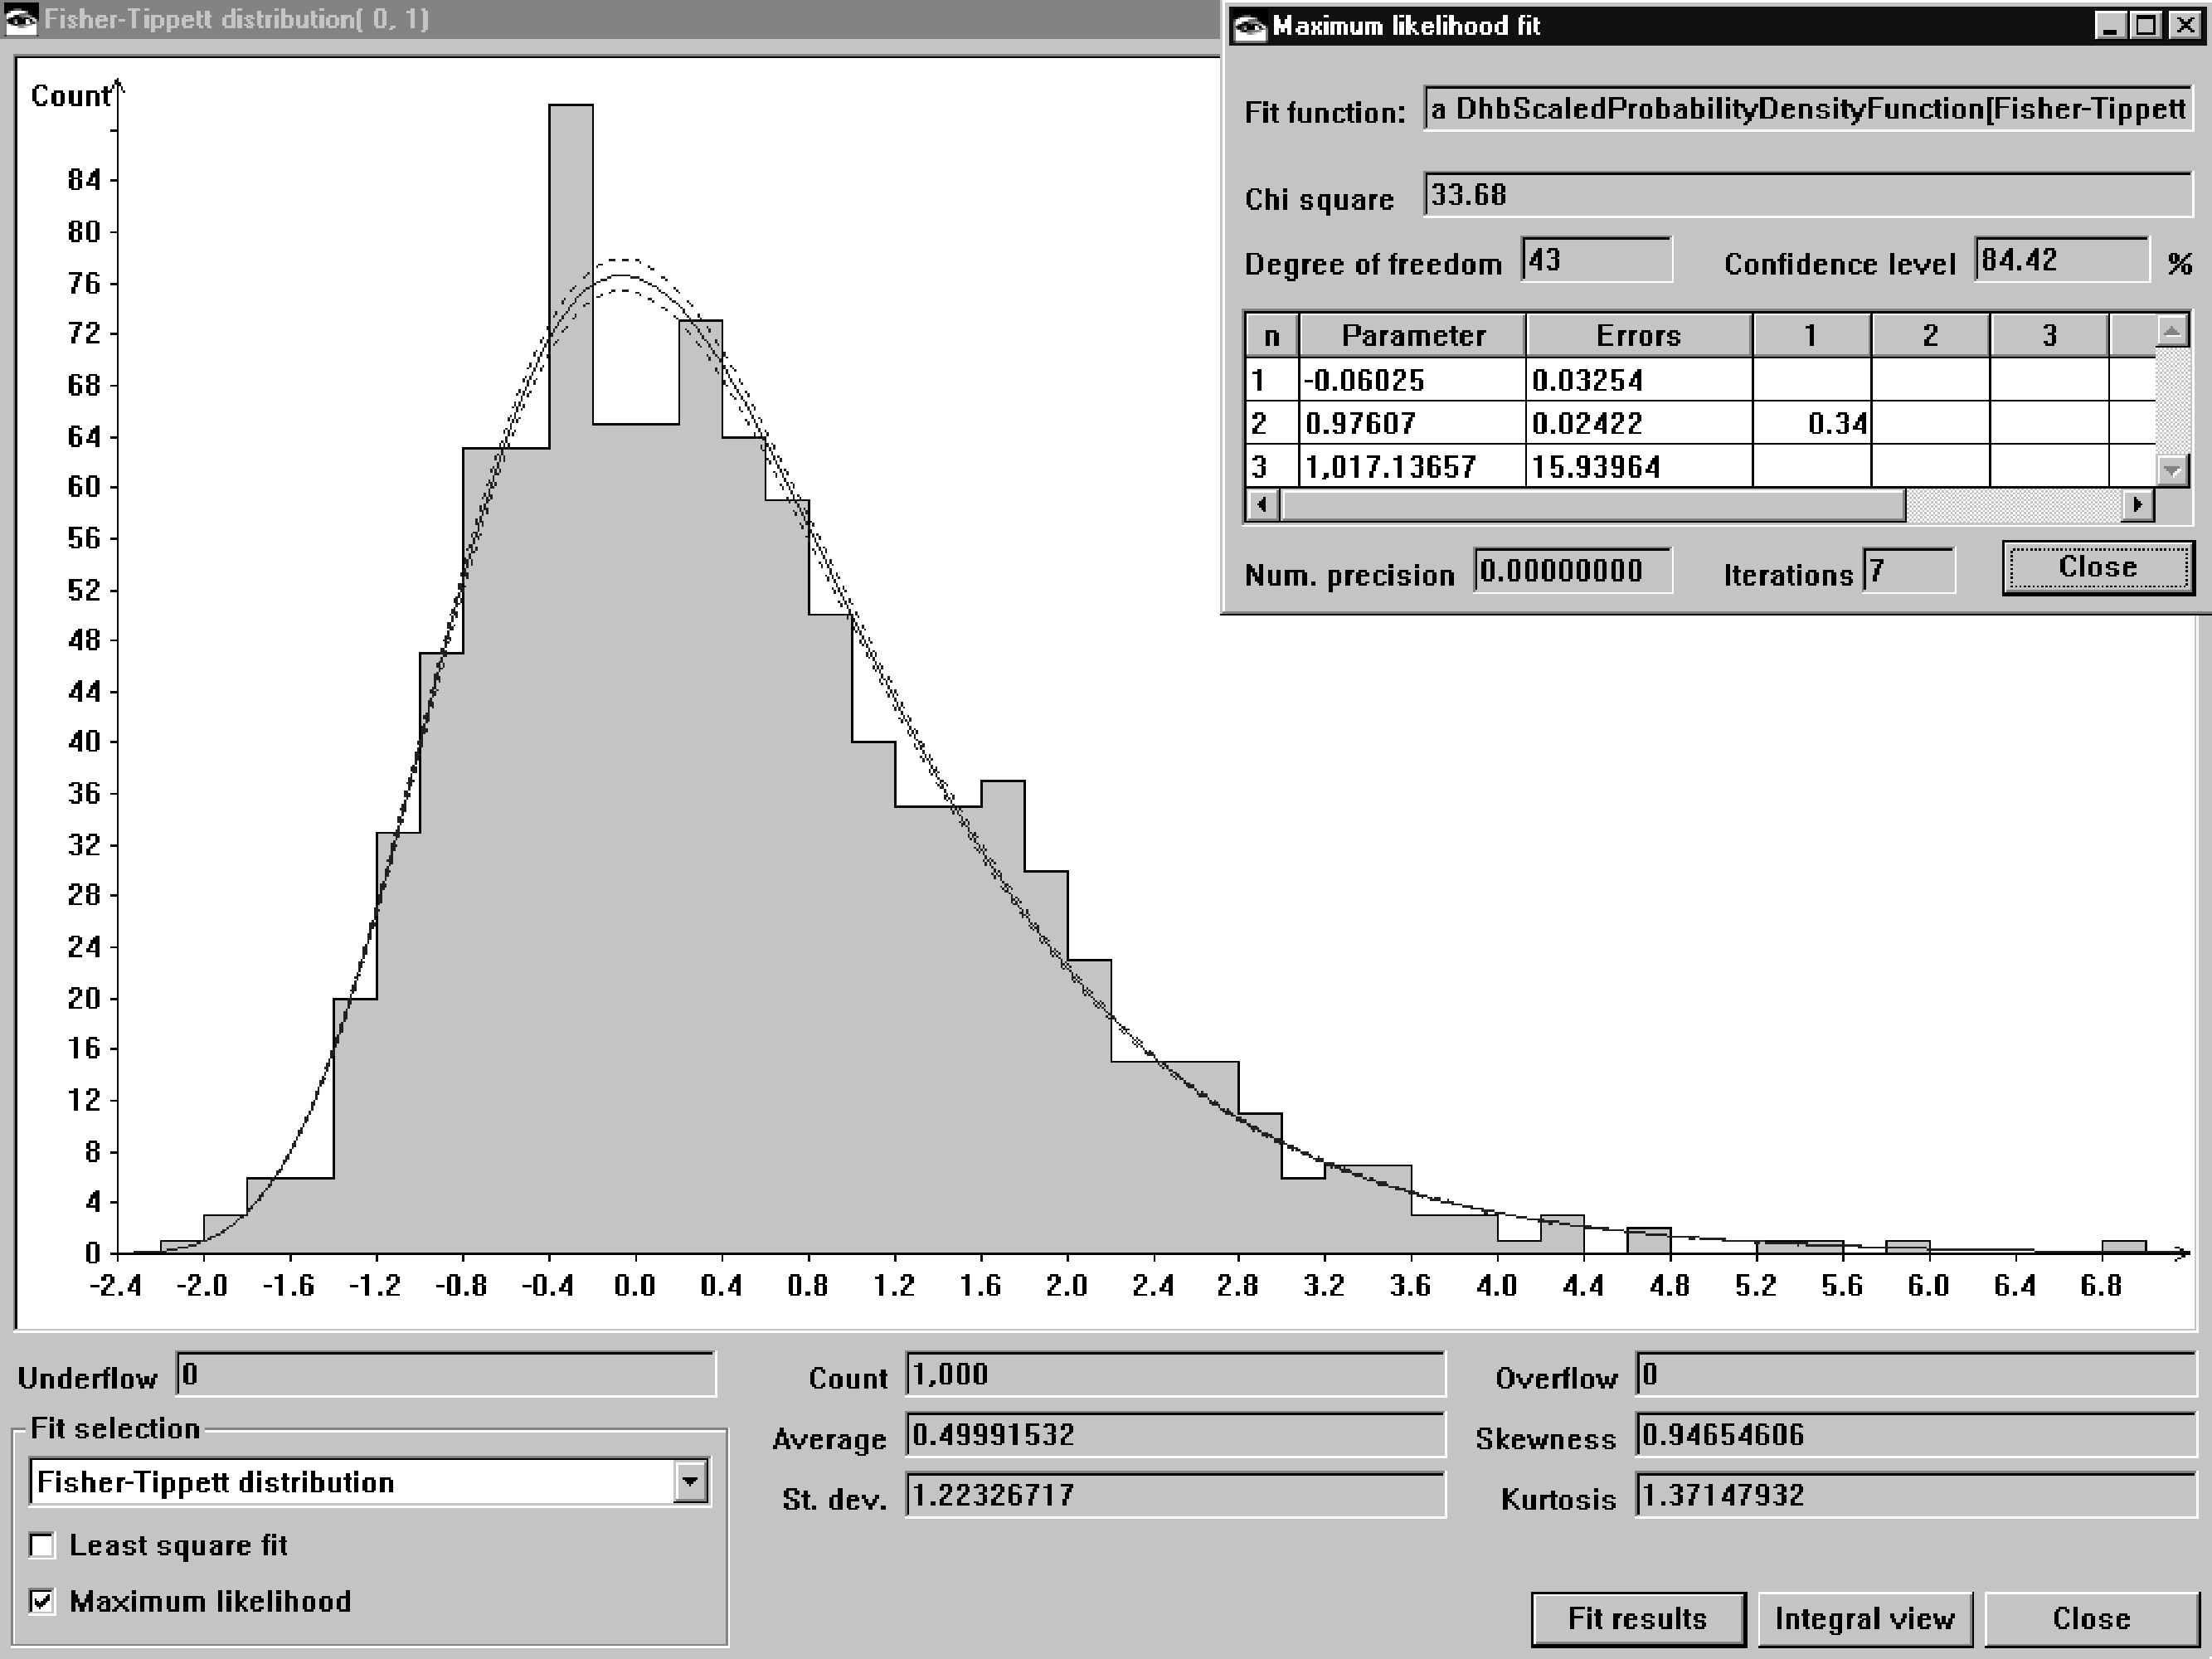
\includegraphics[width=11cm]{Figures/MaximumLikelihoodFit}
\caption{Example of a maximum likelihood
fit}\label{fig:mlfExample}
\end{figure}
The inset window in the upper right corner shows the fit resultsin
the same order as figure \ref{fig:lsfExample}. The correlation
coefficients, however, are not shown for the normalization since
it is not determined as part of the fit. The solid curve laid onto
the histogram is the prediction of the fitted function; the two
dotted lines indicate the error on the prediction. The reader can
see that the fit is as good as the least square fit. Of course,
the $\chi^2$ test is significantly higher with a correspondingly
lower confidence level. This mostly comes from the fact that a
maximum likelihood fit does not use the bins with zero count. In
fact, the reader can see that the count in the histogram
(normalization) estimated by the maximum likelihood fit is higher
than in the case of the least square fit.

\subsection{Maximum likelihood fit --- General  implementation}
\marginpar{Figure \ref{fig:estimationclasses} with the box {\textbf
MaximumLikekihoodHistogramFit} grayed.} A maximum likelihood fit
of a probability density function on a histogram is very similar
to a least square fit of a histogram with a scaled probability
distribution. There are two major differences: first the number of
parameters is lower; second the computation of the matrix and
vectors is not the same. Otherwise, most of the structure of a
least square fit can be reused.

Instead of creating special methods to compute the gradient of the
fitted function using a new set of parameters, our implementation
uses the same gradient calculation than the one used by the least
square fit. This is possible if the component of the gradient
relative to the normalization is placed at the end. Since the
computation of this component does not require additional
calculation, the additional time required by the re-using of the
gradient's computation is negligible. Since the fit function is a
scaled probability distribution the current normalization is kept
in an instance variable and the normalization of the fitted
function is set to 1 for the duration of the iterations. When the
algorithm is completed, the estimated normalization is put back
into the fit function.

The computation of the normalization (equation
\ref{eq:mlfnormsol}) and that of its error (equation
\ref{eq:mlfnormsigma}) is performed in the method {\texttt
finalizeIterations}.

\subsection{Maximum likelihood fit --- Smalltalk  implementation}
\label{sec:smlfhist}Listing \ref{ls:mlf} shows the complete
implementation in Smalltalk. The following code example shows how
figure \ref{fig:mlfExample} was generated up to the plotting
facilities.
\begin{displaycode}{Smalltalk}
 | genDistr hist fit |
 hist := PMHistogram new.
 hist freeExtent: true.
 genDistr := PMFisherTippettDistribution shape: 0 scale: 1.
 1000 timesRepeat: [ hist accumulate: genDistr random ].
 fit := PMMaximumLikekihoodHistogramFit histogram: hist
            distributionClass: PMFisherTippettDistribution.
 fit evaluate.
\end{displaycode}
As the reader can see the only difference with code example
\ref{exs:leastSquare} is the name of the class in the statement
where the instance of the fit is created.

\noindent The class {\texttt PMMaximumLikekihoodHistogramFit} is a
subclass of the class {\texttt PMLeastSquareFit}. It has the
following additional instance variables:
\begin{description}
  \item[\texttt count] the estimated normalization, that is $\bar{N}$;
  \item[\texttt countVariance] the estimated variance of $\bar{N}$.
\end{description}
The variance is kept instead of the error because the most
frequent use of this quantity is in computing the estimated error
on the predicted value. In the method {\texttt valueAndError:} this
computation requires the combination of the error of the fit ---
that is, equation \ref{eq:fitError} --- with the error on the
normalization. An accessor method is provided for the variable
{\texttt count}. The method {\texttt normalizationError} calculates the
error on the normalization.

The method {\texttt accumulate:} uses the vector operations to
calculate the terms of the sums in equations \ref{eq:mlfmatrix}
and \ref{eq:mlfvector}. Because of the lower number of parameters,
the routine {\texttt computeChanges:} places in the vector
$\Delta_{\textbf p}$ an additional zero element corresponding to the
normalization in the case of the least square fit.

The method {\texttt finalizeIterations} calculates the estimated value
of the normalization (equation \ref{eq:mlfnorm}) and its variance
(square of equation \ref{eq:mlfnormsol}). After this, it sets the
obtained normalization into the scaled probability distribution.

\begin{listing} Smalltalk implementation of a maximum likelihood fit \label{ls:mlf}
$$\halign{ #\hfil&\quad#\hfil\cr {\sl Class}& {\Large\bf DhbMaximumLikekihoodHistogramFit}\cr
{\sl Subclass of }&{\tt DhbLeastSquareFit}\cr\noalign{\vskip 1ex}

{\sl Instance variable names:}&\parbox[t]{4 in}{\tt  count countVariance }\cr\noalign{\vskip 1ex}}$$


Instance methods
{\parskip 1ex\par\noindent}
{\bf accumulate:} {\tt aWeightedPoint}
\begin{verbatim}
    | f g temp inverseProbability|
    f := result valueAndGradient: aWeightedPoint xValue.
    g := f last copyFrom: 1 to: ( f last size - 1).
    f := f first.
    f = 0 ifTrue: [ ^nil].
    inverseProbability := 1 / f.
    temp := aWeightedPoint yValue * inverseProbability.
    constants accumulate: g * temp.
    temp := temp * inverseProbability.
    1 to: g size do:
        [ :k |
          ( equations at: k) accumulate: g * ( ( g at: k) * temp).
        ].

\end{verbatim}
{\bf computeChanges}
\begin{verbatim}
    ^super computeChanges copyWith: 0

\end{verbatim}
{\bf computeNormalization}
\begin{verbatim}
    | numerator denominator temp |
    numerator := 0.
    denominator := 0.
    dataHolder pointsAndErrorsDo: 
            [:each | 
            temp := result value: each xValue.
            temp = 0 
                ifFalse: 
                    [numerator := numerator + (each yValue squared / 
                                                                temp).
                    denominator := denominator + temp]].
    count := ( numerator / denominator) sqrt.
    countVariance := numerator / ( 4 * count).

\end{verbatim}
{\bf finalizeIterations}
\begin{verbatim}
    self computeNormalization.
    result setCount: count.
    super finalizeIterations

\end{verbatim}
{\bf fitType}
\begin{verbatim}
    ^'Maximum likelihood fit'

\end{verbatim}
{\bf initializeIterations}
\begin{verbatim}
    result setCount: 1.
    count := dataHolder totalCount.
    super initializeIterations

\end{verbatim}
{\bf normalization}
\begin{verbatim}
    ^count

\end{verbatim}
{\bf normalizationError}
\begin{verbatim}
    ^countVariance sqrt

\end{verbatim}
{\bf numberOfFreeParameters}
\begin{verbatim}
    ^super numberOfParameters

\end{verbatim}
{\bf numberOfParameters}
\begin{verbatim}
    ^super numberOfParameters - 1

\end{verbatim}
{\bf valueAndError:} {\tt aNumber}
\begin{verbatim}
    | valueGradient gradient gVar |
    valueGradient := result valueAndGradient: aNumber.
    gradient := valueGradient last copyFrom: 1 to: valueGradient last 
                                                             size - 1.
    gVar := gradient * (self errorMatrix * gradient) / count.
    ^Array with: valueGradient first
        with: ((valueGradient first / count) squared * countVariance 
                                                          + gVar) sqrt

\end{verbatim}


\end{listing}


%\ifx\wholebook\relax\else\end{document}\fi

%\ifx\wholebook\relax\else
\documentclass[twoside]{book}
\usepackage[active]{srcltx}
\usepackage[LY1]{fontenc}
\usepackage{url}
\makeatletter
\def\url@leostyle{%
  \@ifundefined{selectfont}{\def\UrlFont{\sf}}{\def\UrlFont{\sffamily}}}
\makeatother
% Now actually use the newly defined style.
\urlstyle{leo}

\usepackage{graphicx}
\def\etc{{\textit{etc}}}
\def\eg{{\textit{e.g.}}}
\def\ie{{\textit{i.e.}}}
\def\cf{{\textit{c.f.}}\ }
\def\erf{\mathop{\textrm{erf}}}
\def\sign{\mathop{\textrm{sign}}}
\def\prob{\mathop{\textrm{Prob}}}
\def\var{\mathop{\textrm{var}}}
\def\mod{\mathop{\textrm{mod}}}
\def\cor{\mathop{\textrm{cor}}}
\def\cov{\mathop{\textrm{cov}}}
\def\cl{\mathop{\textrm{CL}}}
\def\kg{\mathop{\textrm{Kg}}}
\def\patstyle#1{{\textsc #1}}
\def\th{^{\mathop{\textrm{th}}}}
%\def\st#1{^{\mathop{\rm #1}}}
\def\note#1{\begin{quote}{\textbf{Note:}} #1\end{quote}}
\def\braket#1{\left\langle #1\right\rangle}
\def\order#1{\let\o=#1$\mathcal{O}$\ifx\o 1$\left(n\right)$\else$\left(n^{#1}\right)$\fi}
%\newtheorem{privListing}{Listing}[chapter]
%\newenvironment{listing}{\vskip 3ex\hrule\vskip 1ex\begin{privListing}}{\end{privListing}\hrule\vskip 1ex}
\newtheorem{privExample}{Code example}[chapter]
\newenvironment{codeExample}{\begin{privExample}\begin{quote}\tt}{\end{quote}\end{privExample}}
\def\relboxl#1#2{\hbox to #1\hsize{#2\hfil}}
\def\relboxc#1#2{\hbox to #1\hsize{\hfil #2\hfil}}
\def\relboxr#1#2{\hbox to #1\hsize{\hfil #2}}
\def\transpose#1{\textbf{#1}^{\mathop\textrm{T}}}
\def\inverse#1{\textbf{#1}^{-1}}
%\def\tm{$^{\mathop{\rm TM}}$}
\def\tm{ }
\newenvironment{mainEquation}{\marginpar[\vspace{3 ex} Main
equation$\Rightarrow$]{\vspace{3 ex}$\Leftarrow$Main
equation}\begin{equation}}{\end{equation}}
\def\rubrique#1{\paragraph{#1}\hfil\par\noindent}

\begin{document}
\fi

\chapter{Optimization}
\label{ch:minimization} \vspace{1 ex}
\begin{flushright}
{\sl Cours vite au but, mais gare \`a la chute.}\footnote{Run fast
to the goal, but beware of the fall.}\\ Alexandre Soljenitsyne
\end{flushright}
\vspace{1 ex} An optimization problem is a numerical problem where
the solution is characterized by the largest or smallest value of
a numerical function depending on several parameters. Such
function is often called the goal function. Many kinds of problems
can be expressed into optimization, that is, finding the maximum
or the minimum of a goal function. This technique has been applied
to a wide variety of fields going from operation research to game
playing or artificial intelligence. In chapter \ref{ch:estimation}
for example, the solution of maximum likelihood or least square
fits was obtained by finding the maximum, respectively the minimum
of a function.

In fact generations of high energy physicists have used the
general purpose minimization program MINUIT\footnote{F.James, M.
Roos, {\sl MINUIT --- a system for function minimization and
analysis of the parameter errors and corrections}, Comput. Phys.
Commun., 10 (1975) 343-367.} written by Fred James\footnote{I take
this opportunity to thank Fred for the many useful discussions we
have had on the subject of minimization.} of CERN to perform least
square fits and maximum likelihood fits.  To achieve generality,
MINUIT uses several strategies to reach a minimum. In this chapter
we shall discuss a few techniques and conclude with a program
quite similar in spirit to MINUIT. Our version, however, will not
have all the features offered by MINUIT.

If the goal function can be expressed with an analytical form, the
problem of optimization can be reduced into calculating the
derivatives of the goal function respective to all parameters, a
tedious but manageable job. In most cases, however, the goal
function cannot always be expressed analytically.

Figure \ref{fig:soptimizingclasses} shows the Smalltalk class diagram.
\begin{figure}
\centering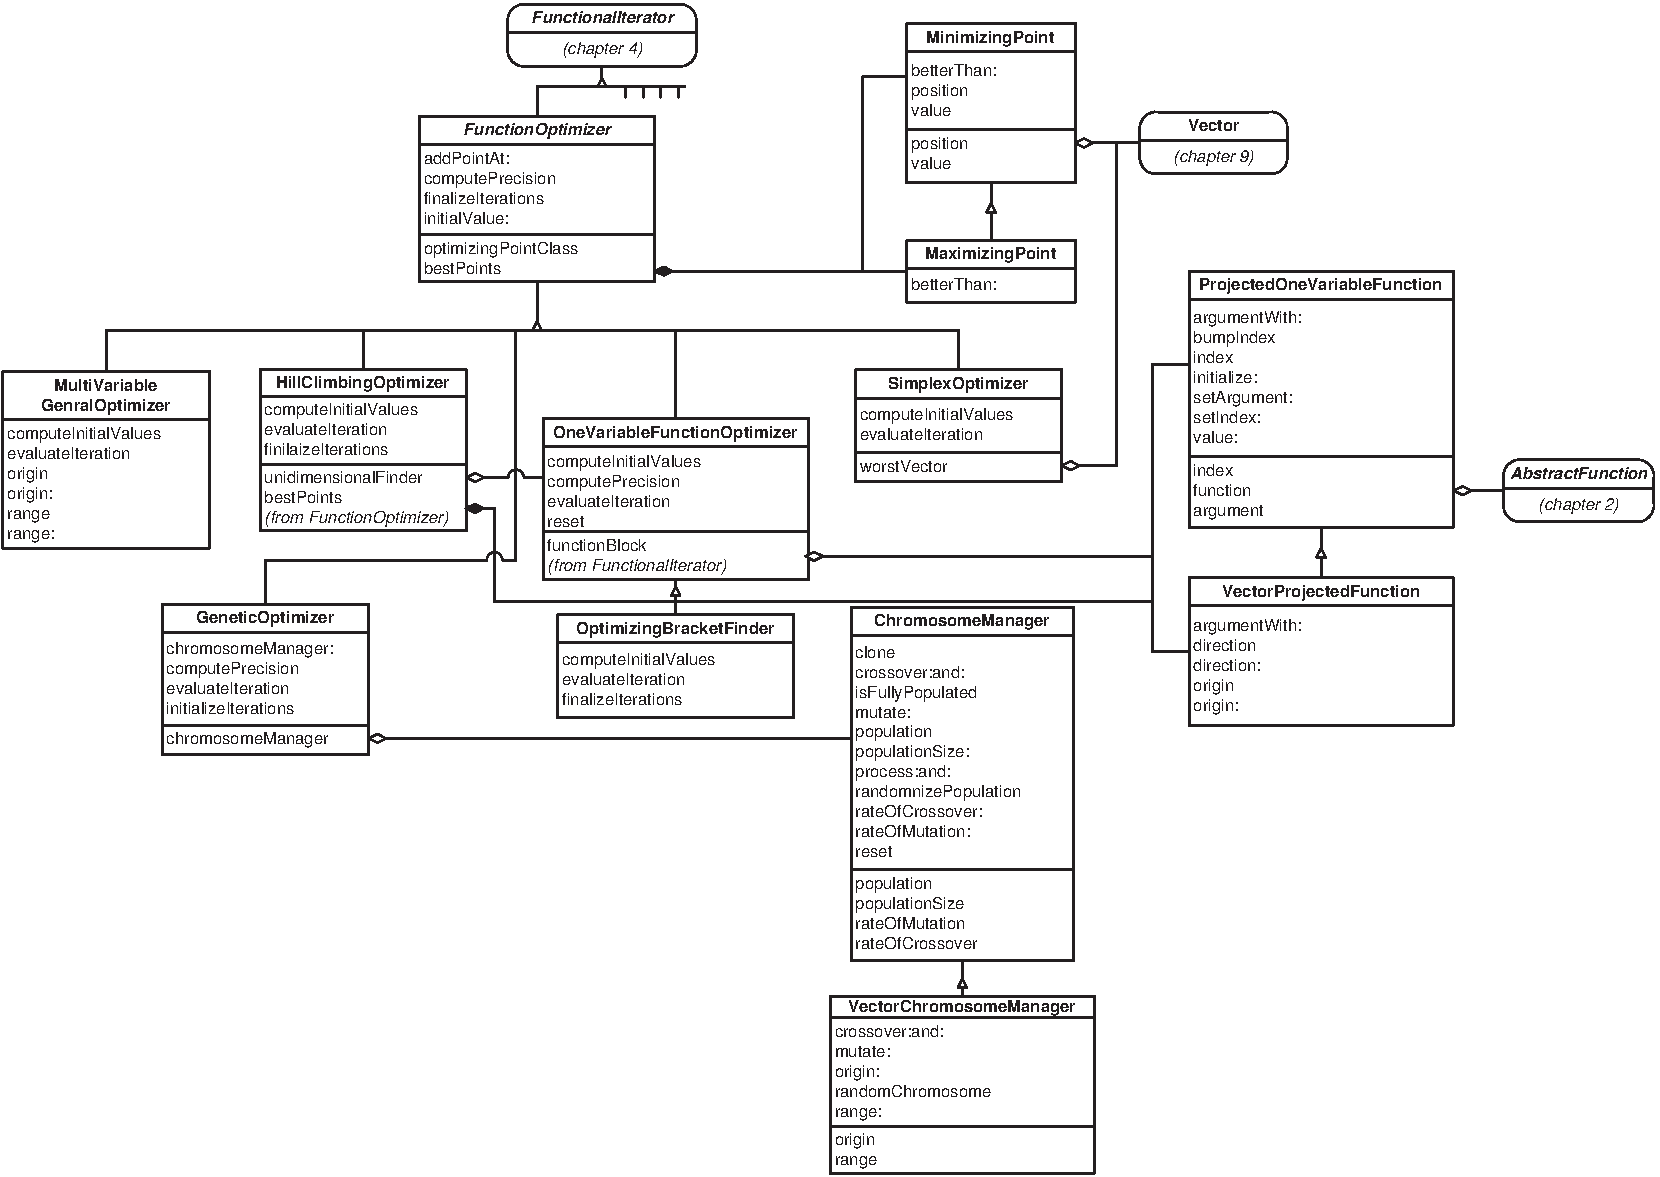
\includegraphics[width=11cm]{Figures/Optimizing}
\caption{Smalltak classes used in optimization}
\label{fig:soptimizingclasses}
\end{figure}

\section{Introduction}
\label{sec:optimum} Let us state the problem is general term. Let
$f\left({\bf x}\right)$ be a function of a vector ${\bf x}$ of
dimension $n$. The $n$-dimensional space is called the search
space of the problem. Depending on the problem the space can be
continuous or not. In this section we shall assume that the space
is continuous.

If the function is derivable, the gradient of the function
respective to the vector ${\bf x}$ must vanish at the optimum.
Finding the optimum of the function can be replaced by the problem
of finding the vector ${\bf x}$ such that:
\begin{equation}
\label{eq:mincondition}
  {d f\left({\bf x}\right) \over d{\bf x}} = 0.
\end{equation}
Unfortunately, the above equation is not a necessary condition for
an optimum. It can be either a maximum. a minimum or a saddle
point, that is a point where the function has a minimum in one
projection and a maximum in another projection. Furthermore, the
function may have several optima. Figure \ref{fig:localabsobulte}
shows an example of a function having two minima.
\begin{figure}
\centering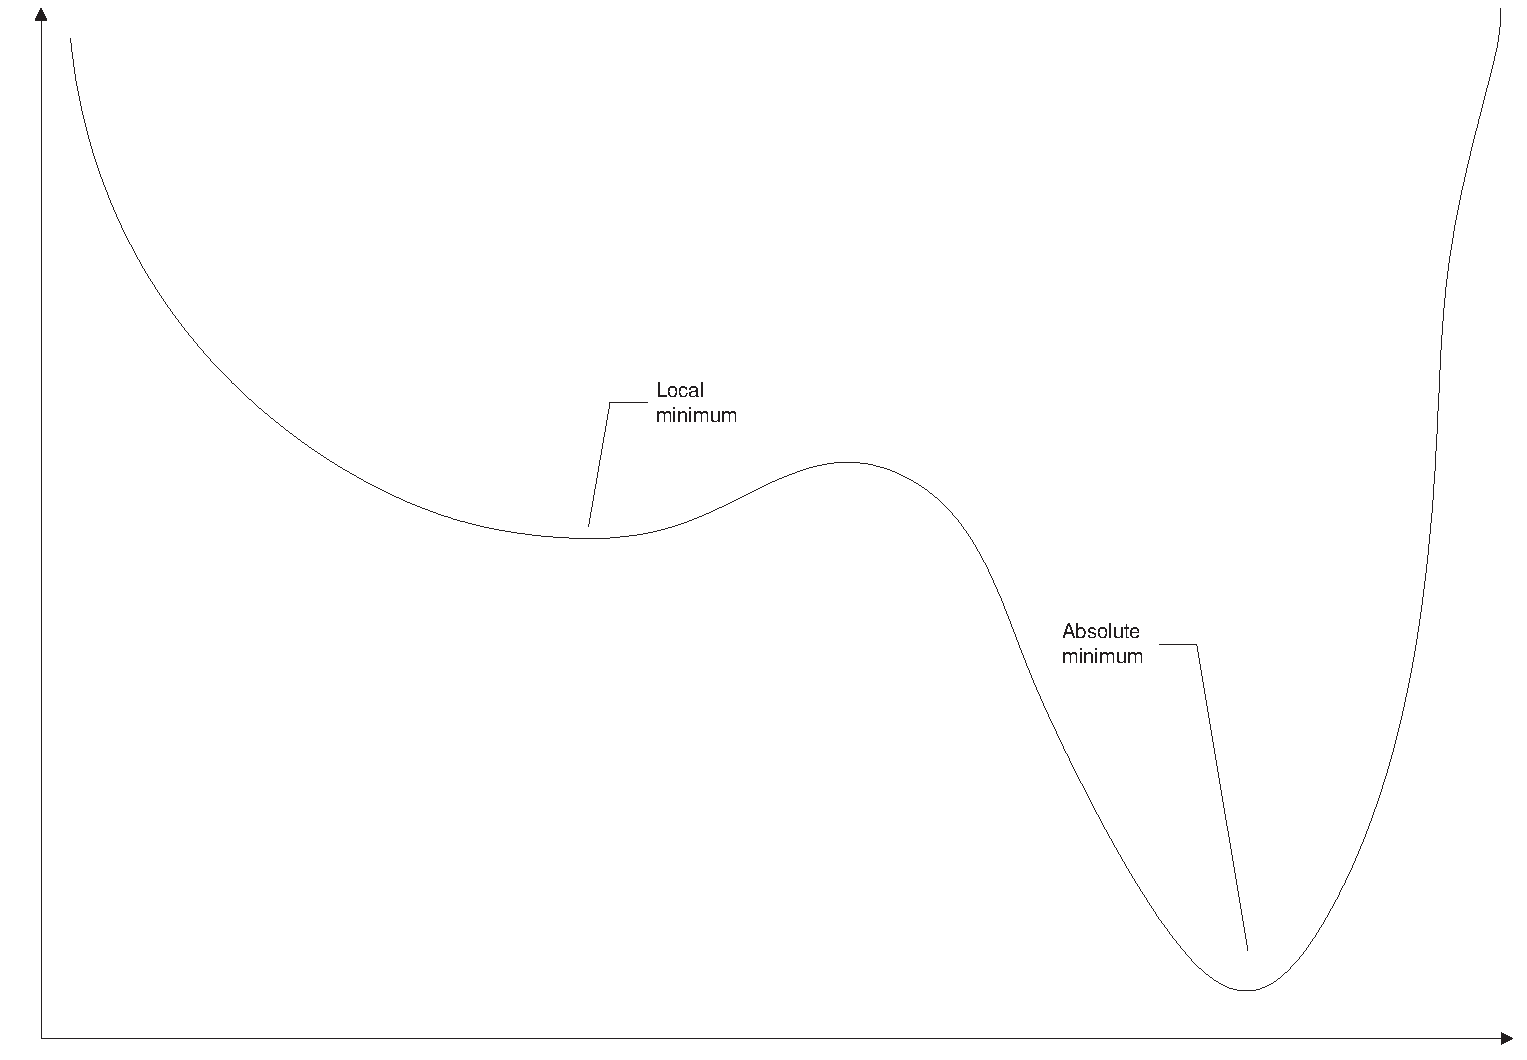
\includegraphics[width=11cm]{Figures/MinimumAbsLoc}
\caption{Local and absolute optima} \label{fig:localabsobulte}
\end{figure}
Some problems require to find the absolute optimum of the
function. Thus, one must verify that the solution of
\ref{eq:mincondition} corresponds indeed to an optimum with the
expected properties. The reader can already see at this point that
searching for an optimum in the general case is a very difficult
task.

\noindent All optimization algorithms can be classified in two
broad categories:
\begin{itemize}
  \item {\sl Greedy algorithms}: these algorithms are characterized by a
  local search in the most promising direction. They are usually efficient
  and quite good at finding local optima. Among greedy algorithms,
  one must distinguish those requiring the evaluation of the
  function's derivatives.
  \item {\sl Random based algorithms}: these algorithms are using
  a random approach. They are not efficient; however, they are good at
  finding absolute optima. Simulated annealing \cite{Press} and
  genetic algorithms\cite{BerLin} belong to this class.
\end{itemize}
The table \ref{tb:optimizingalgorithms} lists the properties of
the algorithms presented in this chapter.
\begin{table}[h]
  \centering
  \caption{Optimizing algorithms presented in this book}\label{tb:optimizingalgorithms}
\vspace{1 ex}\begin{tabular}{| l | c | c |} \hline
  \hfil{\bf Name} & {\bf Category} & {\bf Derivatives} \\ \hline
  Extended Newton & greedy & yes \\
  Powell's hill climbing & greedy & no \\
  Simplex & greedy & no \\
  Genetic algorithm & random based & no \\ \hline
\end{tabular}
\end{table}


\section{Extended Newton algorithms}
Extended Newton algorithms are using a generalized version of
Newton's zero finding algorithm. These algorithms assume that the
function is continuous and has only one optimum in the region
where the search is initiated.

Let us expand the function $f\left({\bf x}\right)$ around a point
${\bf x}^{\left(0\right)}$ near the solution. We have in
components:
\begin{equation}
  f\left({\bf x}\right) = f\left[{\bf x}^{\left(0\right)}\right] +\sum_j
  \left.{\partial f\left({\bf x}\right) \over \partial x_j}\right|_{{\bf x}={\bf
  x}^{\left(0\right)}}
  \left[x_j-x^{\left(0\right)}_j\right].
\end{equation}
Using the expansion above into equation \ref{eq:mincondition}
yields:
\begin{equation}
\sum_j
  \left.{\partial^2 f\left({\bf x}\right) \over \partial x_i\partial x_j}\right|_{{\bf x}={\bf
  x}^{\left(0\right)}}
  \left[x_j-x^{\left(0\right)}_j\right]
  + \left.{\partial f\left({\bf x}\right) \over \partial x_i}\right|_{{\bf x}={\bf
  x}^{\left(0\right)}} =0.
\end{equation}
This equation can be written as a system of linear equations of
the form
\begin{equation}
  {\bf M}\Delta = {\bf c},
\end{equation}
where $\Delta_j =x_j-x^{\left(0\right)}_j$. The components of the
matrix ${\bf M}$ --- called the Hessian matrix --- are given by:
\begin{equation}
  m_{ij} = \left.{\partial^2 f\left({\bf x}\right) \over \partial x_i\partial x_j}\right|_{{\bf x}={\bf
  x}^{\left(0\right)}},
\end{equation}
and the components of the vector ${\bf c}$ are given by:
\begin{equation}
  c_i = -\left.{\partial f\left({\bf x}\right) \over \partial x_i}\right|_{{\bf x}={\bf
  x}^{\left(0\right)}}.
\end{equation}
Like in section \ref{sec:lsfnonlin} one can iterate this process
by replacing ${\bf x}^{\left(0\right)}$ with ${\bf
x}^{\left(0\right)}+\Delta$. This process is actually equivalent
to the Newton zero finding method (\cf section \ref{sec:newton}).
The final solution is a minimum if the matrix ${\bf M}$ is
positive definite; else it is a maximum.

This technique is used by MINUIT in the vicinity of the goal
function's optimum. It is the region where the algorithm described
above works well. Far from the optimum, the risk of reaching a
point where the matrix ${\bf M}$ cannot be inverted is quite high
in general. In addition, the extended Newton algorithm requires
that the second order derivatives of the function can be computed
analytically; at least the first order derivatives must be
provided, otherwise the cost of computation at each step becomes
prohibitive. A concrete implementation of the technique is not
given here. The reader can find in this book all the necessary
tools to make such an implementation. It is left as a exercise for
the reader. In the rest of this chapter, we shall present other
methods which work without an analytical knowledge of the
function.

\section{Hill climbing algorithms}
Hill climbing is a generic term covering many algorithms trying to
reach an optimum by determining the optimum along successive
directions. The general algorithm is outlined below.
\begin{enumerate}
  \item select an initial point ${\bf x}_0$ and a direction ${\bf v}$;
  \item find ${\bf x}_1$, the optimum of the function along the selected
  direction;
  \item if convergence is attained, terminate the algorithm;
  \item set ${\bf x}_0={\bf x}_1$, select a different direction and go back to step 2.
\end{enumerate}
The simplest of these algorithms simply follows each axis in turn
until a convergence is reached. More elaborate algorithms
exist\cite{Press}. One of them is described in section
\ref{sec:powell}.

Hill climbing algorithms can be applied to any continuous
function, especially when the function's derivatives are not
easily calculated. The core of the hill climbing algorithm is
finding the optimum along one direction. Let ${\bf v}$ be the
direction, then finding the optimum of the vector function
$f\left({\bf x}\right)$ along the direction ${\bf v}$ starting
from point ${\bf x}_0$ is equivalent to finding the optimum of the
one-variable function $g\left(\lambda\right)=f\left({\bf
x}_0+\lambda{\bf v}\right)$.

Therefore, in order to implement a hill climbing algorithm, we
first need to implement an algorithm able to find the optimum of a
one-variable function. This is the topic of the sections
\ref{sec:optonedim} and \ref{sec:bracket}. Before this, we need to
discuss the implementation details providing a common framework to
all classes discussed in the rest of this chapter.

\subsection{Optimizing --- General implementation}
\label{sec:goptonedim} At this point the reader may be a little
puzzled by the use of {\sl optimum} instead of speaking of minimum
or maximum. We shall now disclose a general implementation which
works both for finding a minimum or a maximum. This should not
come to a surprise since, in mathematics, a minimum or a maximum
are both very similar --- position where the derivative of a
function vanishes
--- and can be easily turned into each other --- e.g. by negating the
function.

To implement a general purpose optimizing framework, we introduce
two new classes: {\tt MinimizingPoint} and {\tt MaximizingPoint},
 a subclass of {\tt MinimizingPoint}. These two classes
are used as \patstyle{Strategy} by the optimizing algorithms. The
class {\tt MinimizingPoint} has two instance variables
\begin{description}
  \item[\tt value] the value of the goal function, that is
  $g\left(\lambda\right)$ or $f\left({\bf x}\right)$;
  \item[\tt position] the position at which the function has been
  evaluated, that is $\lambda$ or ${\bf x}$.
\end{description}
The class {\tt MinimizingPoint} contains most of the methods. The
only method overloaded by the class  {\tt MaximizingPoint} is the
method {\tt betterThan}, which tells whether an optimizing point
is better than another. The method {\tt betterThan} can be used in
all parts of the optimizing algorithms to find out which point is
the optimum so far. In algorithms working in multiple dimensions,
the method {\tt betterThan} is also used to sort the points from
the best to the worst.

A convenience instance creation method allows to create instances
for a given function with a given argument. The instance is then
initialized with the function's value evaluated at the argument.
Thus, all optimizing algorithms described here do not call the
goal function explicitly.

Otherwise the implementation of the one dimensional optimum search
uses the general framework of the iterative process. More
specifically it uses the class {\tt FunctionalIterator} described
in section \ref{sec:iterrel}.

A final remark concerns the method {\tt initializeIteration}. The
golden search algorithm assume that the 3 points $\lambda_0$,
$\lambda_1$ and $\lambda_2$ have been determined. What if they
have not been? In this case, the method {\tt initializeIteration}
uses the optimum bracket finder described in section
\ref{sec:bracket}

\subsection{Common optimizing classes --- Smalltalk implementation}
\label{sec:sgeneralOpt} \marginpar{Figure
\ref{fig:soptimizingclasses} with the boxes {\bf
FunctionOptimizer}, {\bf MinimizingPoint}, {\bf MaximizingPoint},
{\bf ProjectedOneVariableFunction} and {\bf
VectorProjectedFunction} grayed.} In Smalltalk we have two classes
of optimizing points: {\tt DhbMinimizingPoint} and its subclass
{\tt DhbMaximizingPoint}. These classes are shown in listing
\ref{ls:optimizerCommon}. The class {\tt DhbFunctionOptimizer} is
in charge of handling the management of the optimizing points.
This clas is shown in listing \ref{ls:optimizerAbstract}.

\noindent The class {\tt DhbMinimizingPoint} has the following
instance variables:
\begin{description}
  \item[\tt position] contains the position at which the function
  is evaluated; this instance variable is a number if the function
  to optimize is a one variable function and an array or a vector
  if the function to evaluate is a function of many variables;
  \item[\tt value] contains the value of the function evaluated at the point's position;
\end{description}
Accessor methods corresponding to these variables are supplied. As
we noted in section \ref{sec:goptonedim}, the only method
redefined by the subclass {\tt DhbMaximizingPoint} is the method
{\tt betterThan:} used to decide whether a point is better than
another.

Optimizing points are created with the convenience method {\tt
vector:function:} which evaluates the function supplied as second
argument at the position supplied as the first argument.
\begin{listing} Smalltalk classes common to all optimizing classes \label{ls:optimizerCommon}
$$\halign{ #\hfil&\quad#\hfil\cr {\sl Class}& {\Large\bf DhbMinimizingPoint}\cr
{\sl Subclass of }&{\tt Object}\cr\noalign{\vskip 1ex}

{\sl Instance variable names:}&\parbox[t]{4 in}{\tt  value position }\cr\noalign{\vskip 1ex}}$$


Class methods
{\parskip 1ex\par\noindent}
{\bf new:} {\tt aVector} {\bf value:} {\tt aNumber}
\begin{verbatim}
    ^ self new vector: aVector; value: aNumber; yourself
\end{verbatim}
{\bf vector:} {\tt aVector} {\bf function:} {\tt aFunction}
\begin{verbatim}
    ^ self new: aVector value: (aFunction value: aVector)
\end{verbatim}

Instance methods
{\parskip 1ex\par\noindent}
{\bf betterThan:} {\tt anOptimizingPoint}
\begin{verbatim}
    ^ value < anOptimizingPoint value
\end{verbatim}
{\bf position}
\begin{verbatim}
    ^ position
\end{verbatim}
{\bf printOn:} {\tt aStream}
\begin{verbatim}
    position printOn: aStream.
    aStream
        nextPut: $:;
        space.
    value printOn: aStream
\end{verbatim}
{\bf value}
\begin{verbatim}
    ^ value
\end{verbatim}
{\bf value:} {\tt aNumber}
\begin{verbatim}
    value := aNumber.
\end{verbatim}
{\bf vector:} {\tt aVector}
\begin{verbatim}
    position := aVector
\end{verbatim}


$$\halign{ #\hfil&\quad#\hfil\cr {\sl Class}& {\Large\bf DhbMaximizingPoint}\cr
{\sl Subclass of }&{\tt DhbMinimizingPoint}\cr\noalign{\vskip 1ex}
}$$


Instance methods
{\parskip 1ex\par\noindent}
{\bf betterThan:} {\tt anOptimizingPoint}
\begin{verbatim}
    ^ value > anOptimizingPoint value
\end{verbatim}


\end{listing}

The class {\tt DhbFunctionOptimizer} is in charge of handling the
optimizing points. it has the following instance variables:
\begin{description}
  \item[\tt optimizingPointClass] is the class of the optimizing
  points used as \patstyle{Strategy} by the optimizer; it is used
  to create instances of points at a given position for a given
  function;
  \item[\tt bestPoints] contains a sorted collection of optimizing
  points; the best point is the first and the worst point is the
  last; all optimizers rely on the fact that sorting is done by this sorted collection.
\end{description}
The method {\tt addPointAt:} creates an optimizing point at the
position supplied as argument and adds this point to the
collection of best points. Since that collection is sorted, one is
always certain to find the best result in the first position. This
fact is used by the method {\tt finalizeIterations}, which
retrieves the result from the collection of best points.

Instances of the function optimizer are created with the two
convenience methods {\tt minimizingFuntion:} and {\tt
maximizingFuntion:} helping to define the type of optimum. An
additional convenience method, {\tt forOptimizer:} allows to
create a new optimizer with the same strategy --- that is, the
same class of optimizing points --- and the same function as the
optimizer supplied as argument. This method is used to create
optimizers used in intermediate steps.

Because finding an optimum cannot be determined numerically with
high precision \cite{Press} the class {\tt DhbFunctionOptimizer}
redefines the method {\tt defaultPrecision} to be 100 times the
default numerical precision.
\begin{listing} Smalltalk abstract class for all optimizing classes \label{ls:optimizerAbstract}
$$\halign{ #\hfil&\quad#\hfil\cr {\sl Class}& {\Large\bf DhbFunctionOptimizer}\cr
{\sl Subclass of }&{\tt DhbFunctionalIterator}\cr\noalign{\vskip 1ex}

{\sl Instance variable names:}&\parbox[t]{4 in}{\tt  optimizingPointClass bestPoints }\cr\noalign{\vskip 1ex}}$$


Class methods
{\parskip 1ex\par\noindent}
{\bf defaultPrecision}
\begin{verbatim}
    ^ super defaultPrecision * 100
\end{verbatim}
{\bf forOptimizer:} {\tt aFunctionOptimizer}
\begin{verbatim}
    ^ self new initializeForOptimizer: aFunctionOptimizer
\end{verbatim}
{\bf maximizingFunction:} {\tt aFunction}
\begin{verbatim}
    ^ super new initializeAsMaximizer; setFunction: aFunction
\end{verbatim}
{\bf minimizingFunction:} {\tt aFunction}
\begin{verbatim}
    ^ super new initializeAsMinimizer; setFunction: aFunction
\end{verbatim}



Instance methods
{\parskip 1ex\par\noindent}
{\bf addPointAt:} {\tt aNumber}
\begin{verbatim}
    bestPoints add: (optimizingPointClass vector: aNumber
                                        function: functionBlock)
\end{verbatim}
{\bf bestPoints}
\begin{verbatim}
    ^ bestPoints
\end{verbatim}
{\bf finalizeIterations}
\begin{verbatim}
    result := bestPoints first position.
\end{verbatim}
{\bf functionBlock}
\begin{verbatim}
    ^ functionBlock
\end{verbatim}
{\bf initialize}
\begin{verbatim}
    bestPoints := SortedCollection sortBlock:
                                         [ :a :b | a betterThan: b ].
    ^ super initialize
\end{verbatim}
{\bf initializeAsMaximizer}
\begin{verbatim}
    optimizingPointClass := DhbMaximizingPoint.
    ^ self initialize
\end{verbatim}
{\bf initializeAsMinimizer}
\begin{verbatim}
    optimizingPointClass := DhbMinimizingPoint.
    ^ self
\end{verbatim}
{\bf initializeForOptimizer:} {\tt aFunctionOptimizer}
\begin{verbatim}
    optimizingPointClass := aFunctionOptimizer pointClass.
    functionBlock := aFunctionOptimizer functionBlock.
    ^ self initialize
\end{verbatim}
{\bf initialValue:} {\tt aVector}
\begin{verbatim}
    result := aVector copy.
\end{verbatim}
{\bf pointClass}
\begin{verbatim}
    ^ optimizingPointClass
\end{verbatim}
{\bf printOn:} {\tt aStream}
\begin{verbatim}
    super printOn: aStream.
    bestPoints do: [ :each | aStream cr. each printOn: aStream ].
\end{verbatim}

\end{listing}

In order to find an optimum along a given direction, one needs to
construct an object able to transform a vector function into a one
variable function. The class {\tt DhbProjectedOneVariableFunction}
and its subclass {\tt DhbVectorProjectedFunction} provide this
functionality. They are shown in listing
\ref{ls:projectedfunctions}. The class {\tt
DhbProjectedOneVariableFunction} has the following instance
variables:
\begin{description}
  \item[\tt function] the goal function $f\left({\bf x}\right)$;
  \item[\tt argument] the vector argument of the goal function,
  that is the vector ${\bf x}$;
  \item[\tt index] the index of the axis along which the function
  is projected.
\end{description}
The instance variables {\tt argument} and {\tt index} can be read
and modified using direct accessor methods. The goal function is
set only at creation time: the instance creation method {\tt
function:} take the goal function as argument. A convenience
method {\tt bumpIndex} allows to alter the index in circular
fashion\footnote{We do not give the implementation of the simplest
of the hill climbing algorithms using alternatively each axes of
the reference system. This implementation, which uses the method
{\tt bumpIndex}, is left as an exercise for the reader.}.

The class {\tt DhbVectorProjectedFunction} has no additional
variables. Instead it is reusing the instance variable {\tt index}
as the direction along which the function is evaluated. For
clarity, the accessor methods have been renamed {\tt direction},
{\tt direction:}, {\tt origin} and {\tt origin:}.

For both classes, the method {\tt argumentAt:} returns the
argument vector for the goal function, that is the vector ${\bf
x}$. The method {\tt value:} returns the value of the function
$g\left(\lambda\right)$ for the supplied argument $\lambda$.

\begin{listing} Smalltalk projected function classes \label{ls:projectedfunctions}
$$\halign{ #\hfil&\quad#\hfil\cr {\sl Class}& {\Large\bf DhbProjectedOneVariableFunction}\cr
{\sl Subclass of }&{\tt Object}\cr\noalign{\vskip 1ex}

{\sl Instance variable names:}&\parbox[t]{4 in}{\tt  index function argument }\cr\noalign{\vskip 1ex}}$$


Class methods
{\parskip 1ex\par\noindent}
{\bf function:} {\tt aVectorFunction}
\begin{verbatim}
    ^ super new initialize: aVectorFunction
\end{verbatim}


Instance methods
{\parskip 1ex\par\noindent}
{\bf argumentWith:} {\tt aNumber}
\begin{verbatim}
    ^ argument at: index put: aNumber; yourself
\end{verbatim}
{\bf bumpIndex}
\begin{verbatim}
    index isNil
        ifTrue: [ index := 1]
        ifFalse: [ index := index + 1.
                  index > argument size
                    ifTrue: [ index := 1].
                ].
\end{verbatim}
{\bf index}
\begin{verbatim}
    index isNil
        ifTrue: [ index := 1].
    ^ index
\end{verbatim}
{\bf initialize:} {\tt aFunction}
\begin{verbatim}
    function := aFunction.
    ^ self
\end{verbatim}
{\bf setArgument:} {\tt anArrayOrVector}
\begin{verbatim}
    argument := anArrayOrVector copy.
\end{verbatim}
{\bf setIndex:} {\tt anInteger}
\begin{verbatim}
    index := anInteger.
\end{verbatim}
{\bf value:} {\tt aNumber}
\begin{verbatim}
    ^ function value: ( self argumentWith: aNumber)
\end{verbatim}


$$\halign{ #\hfil&\quad#\hfil\cr {\sl Class}& {\Large\bf DhbVectorProjectedFunction}\cr
{\sl Subclass of }&{\tt DhbProjectedOneVariableFunction}\cr\noalign{\vskip 1ex}
}$$


Instance methods
{\parskip 1ex\par\noindent}
{\bf argumentWith:} {\tt aNumber}
\begin{verbatim}
    ^ aNumber * self direction + self origin
\end{verbatim}
{\bf direction}
\begin{verbatim}
    ^ index
\end{verbatim}
{\bf direction:} {\tt aVector}
\begin{verbatim}
    index := aVector.
\end{verbatim}
{\bf origin}
\begin{verbatim}
    ^ argument
\end{verbatim}
{\bf origin:} {\tt aVector}
\begin{verbatim}
    argument := aVector.
\end{verbatim}
{\bf printOn:} {\tt aStream}
\begin{verbatim}
    self origin printOn: aStream.
    aStream nextPutAll: ' ('.
    self direction printOn: aStream.
    aStream nextPut: $).
\end{verbatim}


\end{listing}

\section{Optimizing in one dimension}
\label{sec:optonedim} To find the optimum of a one-variable
function, $g\left(\lambda\right)$, whose derivative is unknown,
the most robust algorithm is an algorithm similar to the bisection
algorithm described in section \ref{sec:bisection}.

Let us assume that we have found three points $\lambda_0$,
$\lambda_1$ and $\lambda_2$ such that
$\lambda_0<\lambda_1<\lambda_2$ and such that
$g\left(\lambda_1\right)$ is better than both
$g\left(\lambda_0\right)$ and $g\left(\lambda_2\right)$. If the
function $g$ is continuous over the interval
$\left[\lambda_0,\lambda_2\right]$, then we are certain that an
optimum of the function is located in the interval
$\left[\lambda_0,\lambda_2\right]$. As for the bisection
algorithm, we shall try to find a new triplet of values with
similar properties while reducing the size of the interval. A
point is picked in the largest of the two intervals
$\left[\lambda_0,\lambda_1\right]$ or
$\left[\lambda_1,\lambda_2\right]$ and is used to reduce the
initial interval.

If $\lambda_1-\lambda_0\leq\lambda_2-\lambda_1$ we compute
$\lambda_4 =\lambda_1 + \omega\left(\lambda_2-\lambda_1\right)$
where $\omega$ is the golden
section\footnote{$\omega={3-\sqrt{5}\over 2}\approx0.38197$} from
Pythagorean lore. Choosing $\omega$ instead of $1/2$ ensures that
successive intervals have the same relative scale. A complete
derivation of this argument can be found in \cite{Press}. If
$\lambda_4$ yields a better function value than $\lambda_1$, the
new triplet of point becomes $\lambda_1$, $\lambda_4$ and
$\lambda_2$; otherwise, the triplet becomes $\lambda_0$,
$\lambda_1$ and $\lambda_4$.

If we have $\lambda_1-\lambda_0>\lambda_2-\lambda_1$ we compute
$\lambda_4 =\lambda_1 + \omega\left(\lambda_0-\lambda_1\right)$.
Then the new triplets can be either $\lambda_0$, $\lambda_4$ and
$\lambda_1$, or $\lambda_4$, $\lambda_1$ and $\lambda_2$.


The reader can verify that the interval decreases steadily
although not as fast as in the case of bisection where the
interval is halved at each iteration. Since the algorithm is using
the golden section it is called golden section search.

By construction the golden section search algorithm makes sure
that the optimum is always located between the points $\lambda_0$
and $\lambda_2$. Thus, at each iteration, the quantity
$\lambda_2-\lambda_0$ give an estimate of the error on the
position of the optimum.

\subsection{Optimizing in one dimension --- Smalltalk implementation}
\marginpar{Figure \ref{fig:soptimizingclasses} with the box {\bf
OneVariableFunctionOptimizer} grayed.} Listing
\ref{ls:optimizerOneDim} shows the class {\tt
DhbOneVariableFunctionOptimizer} implementing the search for an
optimum of a one-variable function using the golden section
search. The following code example shows how to use this class to
find the maximum of the gamma distribution discussed in section
\ref{sec:gammadist}.
\begin{codeExample}
\begin{verbatim}

 | distr finder maximum |
 distr := DhbGammaDistribution shape: 2 scale: 5.
 finder := DhbOneVariableFunctionOptimizer maximizingFunction: distr.
 maximum := finder evaluate.
\end{verbatim}
\end{codeExample}
The first line after the declarations creates a new instance of a
gamma distribution with parameters $\alpha = 2$ and $\beta = 5$.
The next line creates an instance of the optimum finder. The
selector used to create the instance selects a search for a
maximum. The last line is the familiar statement to evaluate the
iterations --- that is, performing the search for the maximum ---
and to retrieve the result. Since no initial value was supplied
the search begins at a random location.

The class {\tt DhbOneVariableFunctionOptimizer} is a subclass of
the class {\tt FunctionOptimizer}. It does not need any additional
instance variables. The golden section is kept as a class variable
and is calculated at the first time it is needed.

At each iteration the method {\tt nextXValue} is used to compute
the next position at which the function is evaluated. This
corresponding new optimizing point is added to the collection of
best points. Then, the method {\tt indexOfOuterPoint} is used to
determine which point must be discarded: it is always the second
point on either side of the best point. The precision of the
result is estimated from the bracketing interval in the method
{\tt computePrecision}, using relative precision (of course!).

The method {\tt addPoint:} of the superclass can be used to supply
an initial bracketing interval. The method {\tt
computeInitialValues} first checks whether a valid bracketing
interval has been supplied into the collection of best points. If
this is not the case, a search for a bracketing interval is
conducted using the class {\tt DhbOptimizingBracketFinder}
described in section \ref{sec:sbracket}. The instance of the
bracket finder is created with the method {\tt forOptimizer:} so
that its strategy and goal function are taken over from the golden
section optimum finder.

\begin{listing} Smalltalk golden section optimum finder \label{ls:optimizerOneDim}
$$\halign{ #\hfil&\quad#\hfil\cr {\sl Class}& {\Large\bf DhbOneVariableFunctionOptimizer}\cr
{\sl Subclass of }&{\tt DhbFunctionOptimizer}\cr\noalign{\vskip 1ex}

{\sl Class variable names:}&\parbox[t]{4 in}{\tt  GoldenSection }\cr\noalign{\vskip 1ex}}$$


Class methods
{\parskip 1ex\par\noindent}
{\bf defaultPrecision}
\begin{verbatim}
    ^ DhbFloatingPointMachine new defaultNumericalPrecision * 10
\end{verbatim}
{\bf goldenSection}
\begin{verbatim}
    GoldenSection isNil ifTrue: [GoldenSection := (3 - 5 sqrt) / 2].
    ^ GoldenSection
\end{verbatim}



Instance methods
{\parskip 1ex\par\noindent}
{\bf computeInitialValues}
\begin{verbatim}
    [ bestPoints size  > 3 ] whileTrue: [ bestPoints removeLast ].
    bestPoints size = 3
        ifTrue: [ self hasBracketingPoints
                    ifFalse: [ bestPoints removeLast ].
                ].
    bestPoints size < 3
        ifTrue: [ (DhbOptimizingBracketFinder forOptimizer: self) evaluate ].
\end{verbatim}
{\bf computePrecision}
\begin{verbatim}
    ^ self precisionOf: ((bestPoints at: 2) position - (bestPoints 
                                                  at: 3) position) abs
           relativeTo: (bestPoints at: 1) position abs
\end{verbatim}
{\bf evaluateIteration}
\begin{verbatim}
    self addPointAt: self nextXValue.
    bestPoints removeAtIndex: self indexOfOuterPoint.
    ^ self computePrecision
\end{verbatim}
{\bf hasBracketingPoints}
\begin{verbatim}
    | x1 |
    x1 := (bestPoints at: 1) position.
    ^ ((bestPoints at: 2) position - x1) * ((bestPoints at: 3) 
                                                    position - x1) < 0
\end{verbatim}
{\bf indexOfOuterPoint}
\begin{verbatim}
    | inferior superior x |
    inferior := false.
    superior := false.
    x := bestPoints first position.
    2 to: 4 do:
        [ :n |
          (bestPoints at: n) position < x
                ifTrue: [ inferior
                            ifTrue: [ ^ n ].
                          inferior := true.
                        ]
                ifFalse:[ superior
                            ifTrue: [ ^ n ].
                          superior := true.
                        ].
        ].
\end{verbatim}
{\bf nextXValue}
\begin{verbatim}
    | d3 d2 x1 |
    x1 := (bestPoints at: 1) position.
    d2 := (bestPoints at: 2) position - x1.
    d3 := (bestPoints at: 3) position - x1.
    ^ (d3 abs > d2 abs ifTrue: [ d3 ]
                       ifFalse:[ d2 ]) * self class goldenSection + x1
\end{verbatim}
{\bf reset}
\begin{verbatim}
    [ bestPoints isEmpty ] whileFalse: [ bestPoints removeLast ].
\end{verbatim}


\end{listing}

\section{Bracketing the optimum in one dimension}
\label{sec:bracket} As we have seen in section \ref{sec:optonedim}
the golden section algorithm requires the knowledge of a
bracketing interval. This section describes a very simple
algorithm to obtain a bracketing interval with certainty if the
function is continuous and does indeed have an optimum of the
sought type.

The algorithm goes as follows. Take two points $\lambda_0$ and
$\lambda_1$. If they do not exist, pick up some random values
(random generators are described in section \ref{sec:random}). Let
us assume that $g\left(\lambda_1\right)$ is better than
$g\left(\lambda_0\right)$.
\begin{enumerate}
  \item Let $\lambda_2=3\lambda_1-2\lambda_0$, that is, $\lambda_2$ is twice as far from $\lambda_1$ than
$\lambda_0$ and is located on the other side, toward the optimum.
  \item If $g\left(\lambda_1\right)$ is better than
$g\left(\lambda_2\right)$ we have a bracketing interval; the
algorithm is stopped.
  \item Otherwise, set $\lambda_0=\lambda_1$ and $\lambda_1=\lambda_2$ and go back to step 1.
\end{enumerate}
The reader can see that the interval
$\left[\lambda_0,\lambda_1\right]$ is increasing at each step.
Thus, if the function has no optimum of the sought type, the
algorithm will cause a floating overflow exception quite rapidly.

\noindent The implementation in each language have too little in
common. The common section is therefore omitted.

\subsection{Bracketing the optimum --- Smalltalk implementation}
\label{sec:sbracket} \marginpar{Figure
\ref{fig:soptimizingclasses} with the box {\bf
OptimizingBracketFinder} grayed.} Listing
\ref{ls:optimizerbracket} shows the Smalltalk code of the class
implementing the search algorithm for an optimizing bracket. The
class {\tt DhbOptimizingBracketFinder} is a subclass of class {\tt
DhbOneVariableFunctionOptimizer} from section
\ref{ls:optimizerOneDim}. This was a convenient, but not
necessary, choice to be able to reuse most of the management and
accessor methods. The methods pertaining to the algorithm are of
course quite different.

Example of use of the optimizing bracket finder can be found in
method {\tt computeInitialValues} of class {\tt
DhbOneVariableFunctionOptimizer} (\cf listing
\ref{ls:optimizerOneDim}).

The method {\tt setInitialPoints:} allows to use the collection of
best points of another optimizer inside the class. This breach to
the rule of hiding the implementation can be tolerated here
because the class {\tt DhbOptimizingBracketFinder} is used
exclusively with the class {\tt DhbOneVariableFunctionOptimizer}.
It allows the two class to use the same sorted collection of
optimizing points. If no initial point has been supplied, it is
obtained from a random generator.

The {\sl precision} calculated in the method {\tt
evaluateIteration} is a large number, which becomes negative as
soon as the condition to terminate the algorithm is met. Having a
negative precision causes an iterative process as defined in
chapter \ref{ch:iteration} to stop.

\begin{listing} Smalltalk optimum bracket finder \label{ls:optimizerbracket}
$$\halign{ #\hfil&\quad#\hfil\cr {\sl Class}& {\Large\bf DhbOptimizingBracketFinder}\cr
{\sl Subclass of }&{\tt DhbOneVariableFunctionOptimizer}\cr\noalign{\vskip 1ex}
}$$


Class methods
{\parskip 1ex\par\noindent}
{\bf initialPoints:} {\tt aSortedCollection} {\bf function:} {\tt aFunction}
\begin{verbatim}
    ^ super new setInitialPoints: aSortedCollection; setFunction:                                                           aFunction
\end{verbatim}

Instance methods
{\parskip 1ex\par\noindent}
{\bf computeInitialValues}
\begin{verbatim}
    [ bestPoints size < 2 ] whileTrue: [ self addPointAt: Number random ]
\end{verbatim}
{\bf evaluateIteration}
\begin{verbatim}
    | x1 x2 |
    x1 := (bestPoints at: 1) position.
    x2 := (bestPoints at: 2) position.
    self addPointAt: (x1 * 3 - (x2 * 2)).
    precision := (x2 - x1) * ((bestPoints at: 3) position - x1).
    self hasConverged
        ifFalse:[ bestPoints removeLast ].
    ^precision
\end{verbatim}
{\bf finalizeIterations}
\begin{verbatim}
    result := bestPoints.
\end{verbatim}
{\bf initializeForOptimizer:} {\tt aFunctionOptimizer}
\begin{verbatim}
    super initializeForOptimizer: aFunctionOptimizer.
    bestPoints := aFunctionOptimizer bestPoints.
    ^ self
\end{verbatim}
{\bf setInitialPoints:} {\tt aSortedCollection}
\begin{verbatim}
    bestPoints := aSortedCollection.
\end{verbatim}


\end{listing}


\section{Powell's algorithm}
\label{sec:powell}Powell's algorithm is one of many hill climbing
algorithms \cite{Press}. The idea underlying Powell's algorithm is
that once an optimum has been found in one direction, the chance
for the biggest improvement lies in the direction perpendicular to
that direction. A mathematical formulation of this sentence can be
found in \cite{Press} and references therein. Powell's algorithm
provides a way to keep track of the next best direction at each
iteration step.

\noindent The original steps of Powell's algorithm are as follow:
\begin{enumerate}
  \item Let ${\bf x}_0$ the best point so far and initialize a
  series of vectors ${\bf v}_1,\ldots,{\bf v}_n$ forming the system
  of reference ($n$ is the
  dimension of the vector ${\bf x}_0$); in
  other words the components of the vector ${\bf v}_k$ are all
  zero except for the $k\th$ components, which is one.
  \item Set $k=1$.
  \item Find the optimum of the goal function along the direction ${\bf
  v}_k$ starting from point ${\bf x}_{k-1}$. Let ${\bf x}_k$  be
  the position of that optimum.
  \item Set $k=k+1$. If $k\leq n$, go back to step 3.
  \item For $k=1,\ldots,n-1$, set ${\bf v}_k={\bf v}_{k-1}$.
  \item Set ${\bf v}_n ={ {\bf x}_n-{\bf x}_0 \over \left| {\bf x}_n-{\bf x}_0\right|}$.
  \item Find the optimum of the goal function along the direction ${\bf
  v}_n$. Let ${\bf x}_{n+1}$  be the position of that optimum.
  \item If $\left| {\bf x}_n-{\bf x}_0\right|$ is less than the
  desired precision, terminate.
  \item Otherwise, set ${\bf x}_0={\bf x}_{n+1}$ and go back to
  step 1.
\end{enumerate}
There is actually two hill climbing algorithms within each other.
The progression obtained by the inner loop is taken as the
direction in which to continue the search.

Powell recommends to use this algorithm on goal functions having a
quadratic behaviour near the optimum. It is clear that this
algorithm cannot be used safely on any function. If the goal
function has narrow valleys, all directions ${\bf v}_1,\ldots,{\bf
v}_n$ will become colinear when the algorithm ends up in such a
valley. Thus, the search is likely to end up in a position where
no optimum is located. Press et al. \cite{Press} mention two
methods avoiding such problems: one method is quite complex and
the other slows down the convergence of the algorithm.

In spite of this {\it caveat}, we implement Powell's algorithm in
its original form. However, we recommend its use only in the
vicinity of the minimum. In section \ref{sec:multistrategy} we
show how other techniques can be utilized to read the vicinity of
the optimum, where Powell's algorithm can safely be used to make
the final determination of the optimum's position.

\subsection{Powell's algorithm --- General implementation}
Since the class implementing the vector projected function
$g\left(\lambda\right)$ described in section
\ref{sec:sgeneralOpt} keep the vector
${\bf x}_0$ and ${\bf v}$ in instance variables, there is no need
to allocate explicit storage for the vectors ${\bf
x}_1,\ldots,{\bf x}_n$ and ${\bf v}_1,\ldots,{\bf v}_n$. Instead,
the class implementing Powell's algorithm keep an array of vector
projected functions with the corresponding parameters. Then, the
manipulation of the vector ${\bf x}_1,\ldots,{\bf x}_n$ and ${\bf
v}_1,\ldots,{\bf v}_n$ is made directly on the projected function.

Since the origin of the projected function is always the starting
value, ${\bf x}_k$, the initial value for the search of the
optimum of the function $g\left(\lambda\right)$ is always 0.

The method {\tt initializeIterations} allocated a series of vector
projected functions starting with the axes of the reference
system. This method also creates an instance of a one dimensional
optimum finder kept in the instance variable, {\tt
unidimensionalFinder}. The goal function of the finder is
alternatively assigned to each of the projected functions.

We made a slight modification to Powell's algorithm. If the norm
of the vector ${\bf x}_n-{\bf x}_0$ at step 6 is smaller than the
desired precision, the directions are only rotated, the assignment
of step 6 is not done and the search of step 7 is omitted.

The precision computed  at the end of each iterations is the
maximum of the relative change on all components between the
vectors ${\bf x}_n$ and ${\bf x}_0$.

\subsection{Powell's algorithm --- Smalltalk implementation}
\marginpar{Figure \ref{fig:soptimizingclasses} with the box {\bf
HillClimbingOptimizer} grayed.} Listing \ref{ls:optimizerpowell}
shows the implementation of Powell's algorithm in Smalltalk. The
following code example shows how to find the maximum of a vector
function
\begin{codeExample}
\label{ex:spowell}
\begin{verbatim}

 | fBlock educatedGuess hillClimber result |
\end{verbatim}
 {\tt fBlock :=<\sl the goal function\tt >}\hfil\break
 {\tt educatedGuess :=<\sl a vector not too far from the optimum\tt >}
\begin{verbatim}
 hillClimber := DhbHillClimbingOptimizer maximizingFunction: fBlock.
 hillClimber initialValue: educatedGuess.
 result := hillClimber evaluate.
\end{verbatim}
\end{codeExample}
The class {\tt DhbHillClimbingOptimizer} is a subclass of class
{\tt DhbFunctionOptimizer}. It has only one additional instance
variable, {\tt unidimensionalFinder}, to hold the one-dimensional
optimizer used to find an optimum of the goal function along a
given direction.

The method {\tt evaluateIteration} uses the method {\tt
inject:into:} to perform steps 2-4 of the algorithm. Similarly
step 5 of the algorithm is performed with a method {\tt
inject:into:} within the method {\tt shiftDirection}. This mode of
using the iterator method {\tt inject:into:} --- performing an
action involving two consecutive elements of an indexed collection
--- is somewhat unusual, but highly convenient\cite{Beck}. The method {\tt
minimizeDirection:} implements step 3 of the algorithm.

\begin{listing} Smalltalk implementation of Powell's algorithm
\label{ls:optimizerpowell}
$$\halign{ #\hfil&\quad#\hfil\cr {\sl Class}& {\Large\bf DhbHillClimbingOptimizer}\cr
{\sl Subclass of }&{\tt DhbFunctionOptimizer}\cr\noalign{\vskip 1ex}

{\sl Instance variable names:}&\parbox[t]{4 in}{\tt  unidimensionalFinder }\cr\noalign{\vskip 1ex}}$$


Instance methods
{\parskip 1ex\par\noindent}
{\bf computeInitialValues}
\begin{verbatim}
    unidimensionalFinder := DhbOneVariableFunctionOptimizer
                                                   forOptimizer: self.
    unidimensionalFinder desiredPrecision: desiredPrecision.
    bestPoints := (1 to: result size)
                 collect: [ :n | ( DhbVectorProjectedFunction
                                      function: functionBlock)
                                     direction: ((DhbVector
                                                     new: result size)
                                                         atAllPut: 0;
                                                         at: n put: 1;
                                                         yourself);
                                            yourself
                          ].

\end{verbatim}
{\bf evaluateIteration}
\begin{verbatim}
    | oldResult |
    precision := 1.
    bestPoints inject: result
                 into: [ :prev :each | ( self minimizeDirection: each
                                                         from: prev)].
    self shiftDirections.
    self minimizeDirection: bestPoints last.
    oldResult := result.
    result := bestPoints last origin.
    precision := 0.
    result with: oldResult do:
        [ :x0 :x1 |
          precision := ( self precisionOf: (x0 - x1) abs relativeTo:
                                               x0 abs) max: precision.
        ].
    ^ precision
\end{verbatim}
{\bf minimizeDirection:} {\tt aVectorFunction}
\begin{verbatim}
    ^ unidimensionalFinder
        reset;
        setFunction: aVectorFunction;
        addPointAt: 0;
        addPointAt: precision;
        addPointAt: precision negated;
        evaluate
\end{verbatim}
{\bf minimizeDirection:} {\tt aVectorFunction} {\bf from:} {\tt aVector}
\begin{verbatim}
Function from: aVector
    ^aVectorFunction
        origin: aVector;
        argumentWith: (self minimizeDirection: aVectorFunction)
\end{verbatim}
{\bf shiftDirections}
\begin{verbatim}
    | position delta firstDirection |
    firstDirection := bestPoints first direction.
    bestPoints inject: nil
                    into: [ :prev :each |
                            position isNil
                                ifTrue: [ position := each origin]
                                ifFalse:[ prev direction: each
                                                           direction].
                            each
                            ].
    position := bestPoints last origin - position.
    delta := position norm.
    delta > desiredPrecision
        ifTrue: [ bestPoints last direction: (position scaleBy: (1 /
                                                              delta))]
        ifFalse:[ bestPoints last direction: firstDirection].
\end{verbatim}

\end{listing}

\section{Simplex algorithm}
\label{sec:simplex} The simplex algorithm, invented by Nelder and
Mead, provides an efficient way to find a good approximation of
the optimum of a function starting from any place \cite{Press}.
The only trap into which the simplex algorithm can run into is a
local optimum. On the other hand, this algorithm does not converge
very well in the vicinity of the optimum. Thus, it must not be
used with the desired precision set to a very low value. Once the
optimum has been found with the simplex algorithm, other more
precise algorithms can then be used, such as the ones describes in
section \ref{sec:optimum} or \ref{sec:powell}. MINUIT uses a
combination of simplex and Newton algorithms. Our implementation
of general purpose optimizer uses a combination of simplex and
Powell algorithms.

A simplex in a $n$-dimensional space is a figure formed with $n+1$
summits. For example, a simplex in a 2-dimensional space is a
triangle; a simplex in a 3-dimensional space is a tetrahedron.
Let us now discuss the algorithm for finding the optimum of a
function with a simplex.
\begin{enumerate}
  \item Pick up $n+1$ points in the search space and evaluate
  the goal function at each of them. Let ${\bf A}$ be the summit
  yielding the worst function's value.
  \item if the size of the simplex is smaller than the desired
  precision, terminate the algorithm.
  \item Calculate ${\bf G}$, the center of gravity of the $n$ best points,
  that is all points except ${\bf A}$.
  \item Calculate the location of the symmetric point of ${\bf A}$
  relative to ${\bf G}$: ${\bf A}^{\prime}=2{\bf G}-{\bf A}$.
  \item If $f\left({\bf A}^{\prime}\right)$ is not the best value
  found so far go to step 9.
  \item Calculate the point ${\bf A}^{\prime\prime}=2{\bf A}^{\prime}-{\bf
  G}$, that is a point twice as far from ${\bf G}$ as ${\bf
  A}^{\prime}$.
  \item If $f\left({\bf A}^{\prime\prime}\right)$ is a
  better value than $f\left({\bf A}^{\prime}\right)$ build a new
  simplex with the point ${\bf A}$ replaced by the point ${\bf
  A}^{\prime\prime}$ and go to step 2.
  \item Otherwise, build a new
  simplex with the point ${\bf A}$ replaced by the point ${\bf
  A}^{\prime}$ and go to step 2.
  \item Calculate the point ${\bf B}= {\displaystyle\left({\bf G}+{\bf
A}\right)\over\displaystyle 2}$.
  \item If $f\left({\bf B}\right)$ yields the best value found so far
  build a new simplex with the point ${\bf A}$ replaced by the point ${\bf
  A}^{\prime\prime}$ and go to step 2.
  \item Otherwise build a new simplex obtained by dividing all
  edges leading to the point yielding the best value by 2 and go
  back to step 2.
\end{enumerate}
Figure \ref{fig:simplexsample} shows the meaning of the operations
involved in the algorithm in the 3 dimensional case.
\begin{figure}
\centering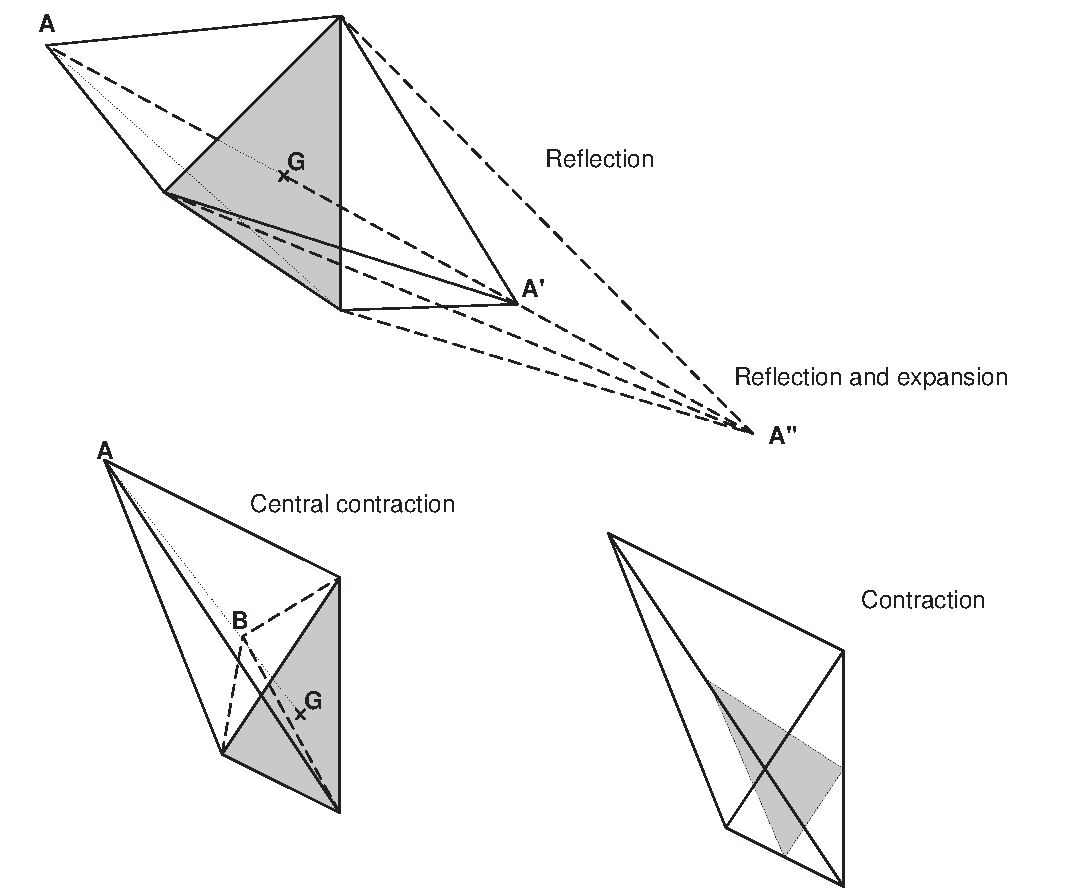
\includegraphics[width=10cm]{Figures/Simplex}
\caption{Operations of the simplex
algorithm}\label{fig:simplexsample}
\end{figure}
Step 6 makes the simplex grow into the direction where the
function is the best so far. Thus, the simplex becomes elongated
in the expected direction of the optimum. Because of its
geometrical shape, the next step is necessarily taken along
another direction, causing an exploration of the regions
surrounding the growth obtained at the preceding step. Over the
iterations, the shape of the simplex adapts itself to narrow
valleys where the hill climbing algorithms notoriously get into
trouble. Steps 9 and 11 ensures the convergence of the algorithm
when the optimum lies inside the simplex. In this mode the simplex
works very much like the golden section search or the bisection
algorithms.

Finding the initial points can be done in several ways. If a good
approximation of the region where the maximum might be located can
be obtained one uses that approximation as a start and generate
$n$ other points by finding the optimum of the function along each
axis. Otherwise, one can generate random points and select $n+1$
points yielding the best values to build the initial simplex. In
all cases, one must make sure that the initial simplex has a
non-vanishing size in all dimensions of the space. Otherwise the
algorithm will not reach the optimum.

\subsection{Simplex algorithm --- General implementation}
The class implementing the simplex algorithm belong to the
hierarchy of the iterative processes discussed in chapter
\ref{ch:iteration}. The method {\tt evaluateIteration} directly
implements the steps of the algorithm as described above. The
points ${\bf G}$, ${\bf A}^{\prime}$, ${\bf A}^{\prime\prime}$ and
${\bf B}$ are calculated using the vector operations described in
section \ref{sec:linearalgebra}.

The routine {\tt initializeIterations} assumes that an initial
value has been provided. It then finds the location of an optimum
of the goal function along each axis of the reference system
starting each time from the supplied initial value, unlike hill
climbing algorithms. Restarting from the initial value is
necessary to avoid creating a simplex with a zero volume. Such
mishaps can arise when the initial value is located on an axis of
symmetry of the goal function. This can happen quite frequently
with {\sl educated guesses}.

\subsection{Simplex algorithm --- Smalltalk implementation}
\marginpar{Figure \ref{fig:soptimizingclasses} with the box {\bf
SimplexOptimizer} grayed.} Listing \ref{ls:optimizersimplex} shows
the Smalltalk implementation of the simplex algorithm. The
following code example shows how to invoke the class to find the
minimum of a vector function.
\begin{codeExample}
\begin{verbatim}

 | fBlock educatedGuess simplex result |
\end{verbatim}
 {\tt fBlock :=<\sl the goal function\tt >}\hfil\break
 {\tt educatedGuess :=<\sl a vector in the search space\tt >}
\begin{verbatim}
 simplex := DhbSimplexOptimizer minimizingFunction: fBlock.
 simplex initialValue: educatedGuess.
 result := simplex evaluate.
\end{verbatim}
\end{codeExample}
Except for the line creating the instance of the simplex
optimizer, this code example is identical to the example of
Powell's hill climbing algorithm (code example \ref{ex:spowell}).

The class {\tt DhbSimplexOptimizer} is a subclass of class {\tt
DhbFunctionOptimizer}. In order to be able to use the iterator
methods efficiently, the worst point of the simplex, ${\bf A}$, is
held in a separate instance variable {\tt worstPoint}. As we do
not need to know the function's value $f\left({\bf A}\right)$, it
is kept as a vector. The remaining points of the simplex are kept
in the instance variable {\tt bestPoints} of the superclass. Since
this collection is sorted automatically when points are inserted
to it, there is no explicit sorting step.

\begin{listing} Smalltalk implementation of simplex algorithm
\label{ls:optimizersimplex}
$$\halign{ #\hfil&\quad#\hfil\cr {\sl Class}& {\Large\bf DhbSimplexOptimizer}\cr
{\sl Subclass of }&{\tt DhbFunctionOptimizer}\cr\noalign{\vskip 1ex}

{\sl Instance variable names:}&\parbox[t]{4 in}{\tt  worstVector }\cr\noalign{\vskip 1ex}}$$


Class methods
{\parskip 1ex\par\noindent}
{\bf defaultPrecision}
\begin{verbatim}
    ^DhbFloatingPointMachine new defaultNumericalPrecision * 1000

\end{verbatim}



Instance methods
{\parskip 1ex\par\noindent}
{\bf buildInitialSimplex}
\begin{verbatim}
    | projectedFunction finder partialResult |
    projectedFunction := DhbProjectedOneVariableFunction 
                function: functionBlock.
    finder := DhbOneVariableFunctionOptimizer forOptimizer: self.
    finder setFunction: projectedFunction.
    [bestPoints size < (result size + 1)] whileTrue: 
            [projectedFunction
                setArgument: result;
                bumpIndex.
            partialResult := finder
                        reset;
                        evaluate.
            bestPoints add: (optimizingPointClass 
                        vector: (projectedFunction argumentWith: 
                                                        partialResult)
                        function: functionBlock)]

\end{verbatim}
{\bf computeInitialValues}
\begin{verbatim}
    bestPoints 
        add: (optimizingPointClass vector: result function: 
                                                       functionBlock).
    self buildInitialSimplex.
    worstVector := bestPoints removeLast position

\end{verbatim}
{\bf computePrecision}
\begin{verbatim}
    | functionValues bestFunctionValue |
    functionValues := bestPoints collect: [ :each | each value].
    bestFunctionValue := functionValues removeFirst.
    ^functionValues inject: 0
                    into: [ :max :each | ( self precisionOf: ( each - 
   bestFunctionValue) abs relativeTo: bestFunctionValue abs) max: max]

\end{verbatim}
{\bf contract}
\begin{verbatim}
    | bestVector oldVectors |
    bestVector := bestPoints first position.
    oldVectors := OrderedCollection with: worstVector.
    [bestPoints size > 1] whileTrue: [oldVectors add: bestPoints 
                                                 removeLast position].
    oldVectors do: [:each | self contract: each around: bestVector].
    worstVector := bestPoints removeLast position.
    ^self computePrecision

\end{verbatim}
{\bf contract:} {\tt aVector} {\bf around:} {\tt bestVector}
\begin{verbatim}
    bestPoints 
        add: (optimizingPointClass vector: bestVector * 0.5 + 
                                                       (aVector * 0.5)
                function: functionBlock)

\end{verbatim}
{\bf evaluateIteration}
\begin{verbatim}
    | centerOfGravity newPoint nextPoint |
    centerOfGravity := (bestPoints inject: ((worstVector copy)
                        atAllPut: 0;
                        yourself)
                into: [:sum :each | each position + sum]) * (1 / 
                                                     bestPoints size).
    newPoint := optimizingPointClass vector: 2 * centerOfGravity - 
                                                           worstVector
                function: functionBlock.
    (newPoint betterThan: bestPoints first) 
        ifTrue: 
            [nextPoint := optimizingPointClass 
                        vector: newPoint position * 2 - 
                                                       centerOfGravity
                        function: functionBlock.
            (nextPoint betterThan: newPoint) ifTrue: [newPoint := 
                                                           nextPoint]]
        ifFalse: 
            [newPoint := optimizingPointClass 
                        vector: centerOfGravity * 0.666667 + 
                                              (worstVector * 0.333333)
                        function: functionBlock.
            (newPoint betterThan: bestPoints first) ifFalse: [^self 
                                                           contract]].
    worstVector := bestPoints removeLast position.
    bestPoints add: newPoint.
    result := bestPoints first position.
    ^self computePrecision

\end{verbatim}
{\bf printOn:} {\tt aStream}
\begin{verbatim}
    super printOn: aStream.
    aStream cr. 
    worstVector printOn: aStream.

\end{verbatim}


\end{listing}

\section{Genetic algorithm}
All optimizing algorithm discussed so far have one common flaw:
they all terminate when a local optimum is encountered. In most
problems, however, one wants to find the absolute optimum of the
function. This is especially true if the goal function represents
some economical merit.

\noindent One academic example is the maximization of the function
\begin{equation}
\label{eq:geneticCase}
  f\left({\bf x}\right)={ \sin^2\left|{\bf x}\right| \over\left|{\bf
  x}\right|^2}.
\end{equation}
This function has an absolute maximum at ${\bf x}=0$, but all
algorithms discussed so far will end up inside a ring
corresponding to $\left|{\bf x}\right|=n\pi/2$ where $n$ is any
positive odd integer.

In 1975 John Holland introduced a new type of algorithm --- dubbed
genetic algorithm --- because it tries to mimic the evolutionary
process identified as the cause for the diversity of living
species by Charles Darwin. In a genetic algorithm the elements of
the search space are considered as the chromosomes of individuals;
the goal function is considered as the measure of the fitness of
the individual to adapt itself to its
environment\cite{BerLin}\cite{Koza}. The iterations are aping (pun
intended) the Darwinian principle of survival and reproduction. At
each iteration, the fittest individuals survive and reproduce
themselves. To bring some variability to the algorithm mutation
and crossover of chromosomes are taken into account.

Mutation occurs when one gene of a chromosome is altered at
reproduction time. Crossover occurs when two chromosomes break
themselves and recombine with the piece coming from the other
chromosome. These processes are illustrated on figure
\ref{fig:crossover}.
\begin{figure}
\centering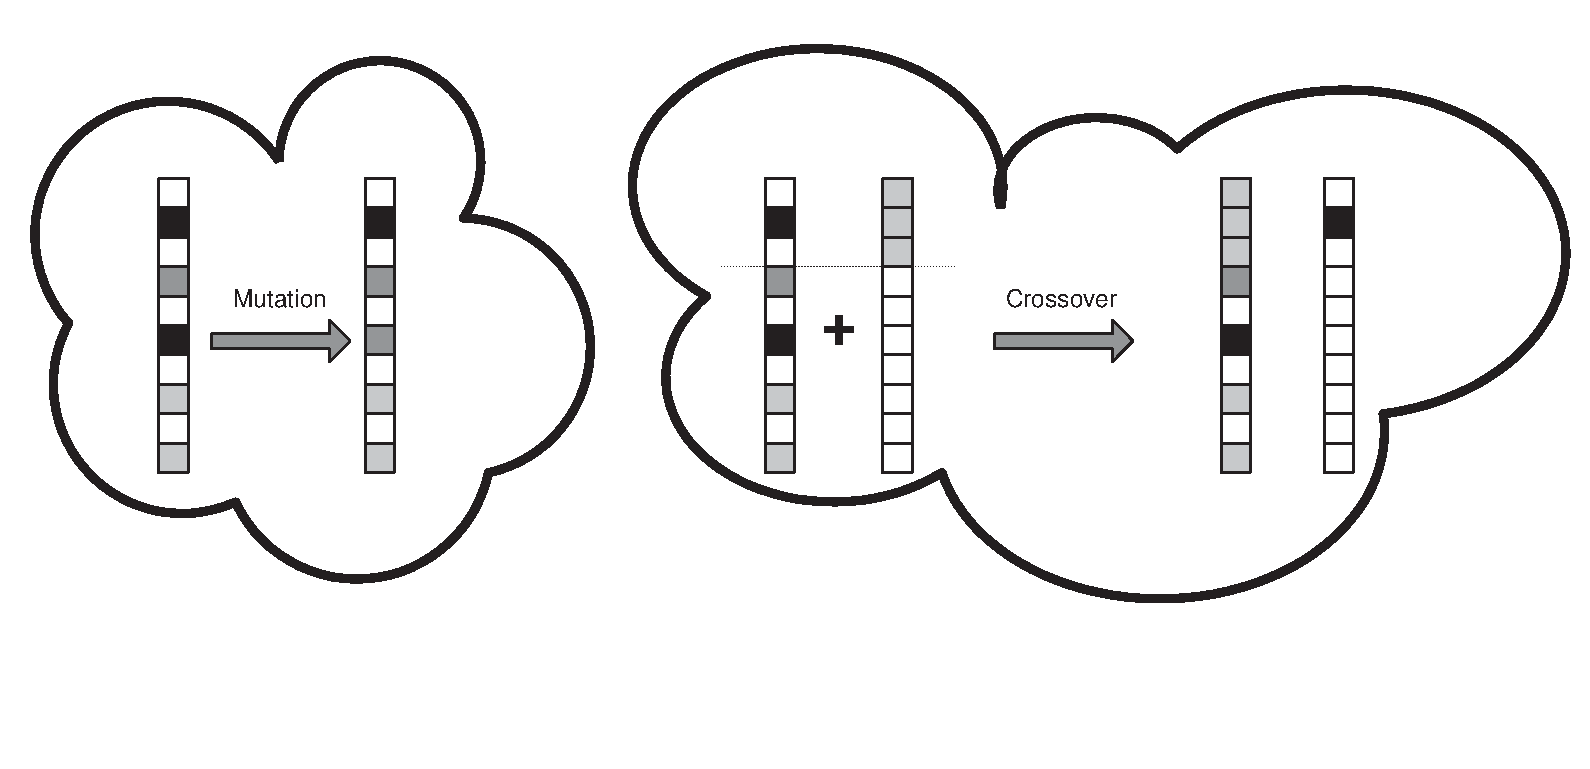
\includegraphics[width=11cm]{Figures/Crossover}
\caption{Mutation and crossover reproduction of
chromosomes}\label{fig:crossover}
\end{figure}
The point where the chromosomes are breaking is called the
crossover point. Which individual survives and reproduces itself,
when and where mutation occurs and when and where a crossover
happens is determined randomly. This is precisely the random
nature of the algorithm which gives it the ability to jump out of
a local optimum to look further for the absolute optimum.

\rubrique{Mapping the search space on chromosomes} To be able to
implement a genetic algorithm one must establish how to represent
the genes of a chromosome. At the smallest level the genes could
be the bits of the structure representing the chromosome. If the
search space of the goal function do cover the domain generated by
all possible permutations of the bits, this is a good approach.
However, this is not always a practical solution since some bit
combinations may be forbidden by the structure. For example, some
of the combinations of a 64 bit word do not correspond to a valid
floating point number.

In the case of the optimization of a vector function, the simplest
choice is to take the components of the vector as the genes.
Genetic algorithms are used quite often to adjust the parameters
of a neural network \cite{BerLin}. In this case, the chromosomes
are the coefficients of each neuron. Chromosomes can even be
computer subprograms in the case of genetic programming
\cite{Koza}. In this latter case, each individual is a computer
program trying to solve a given problem.

Figure \ref{fig:geneticFlow} shows a flow diagram of a general
genetic algorithm.
\begin{figure}
\centering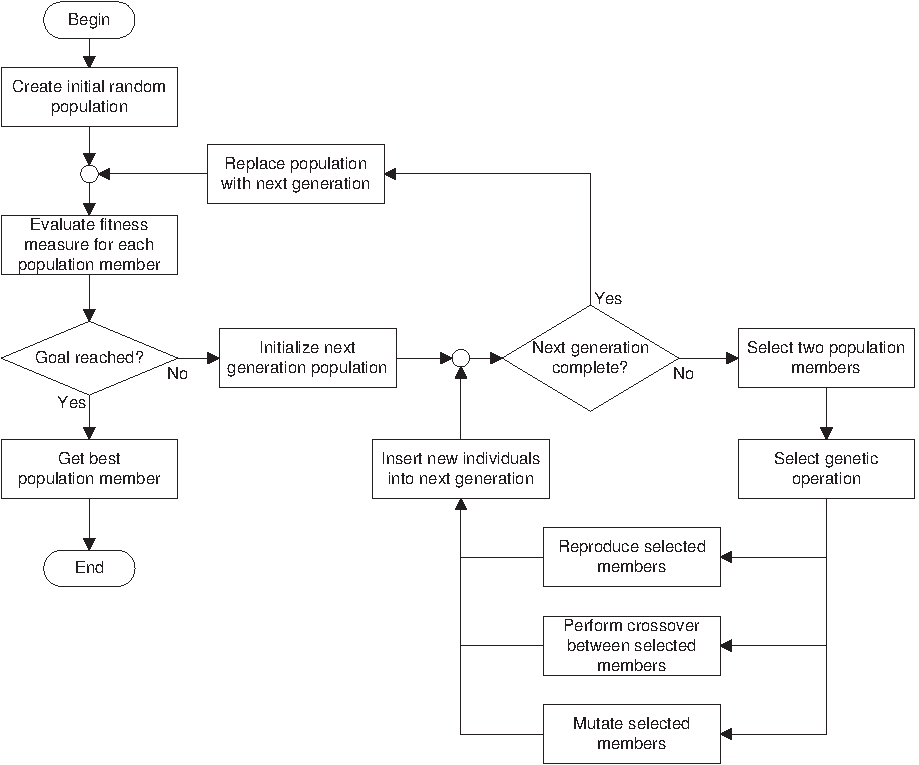
\includegraphics[width=10cm]{Figures/GeneticFlow}
\caption{General purpose genetic algorithm}\label{fig:geneticFlow}
\end{figure}
The reproduction of the individual is taken literally: a copy of
the reproducing individual is copied into the next generation. The
important feature of a generic algorithm is that the building of
the next generation is a random process. To ensure the survival of
the fittest, the selection of the parents of the individuals of
the next generation is performed at random with uneven
probability: the fittest individuals have a larger probability of
being selected than the others. Mutation enables the algorithm to
create individuals having genes corresponding to unexplored
regions of the search space. Most of the times such mutants will
be discarded at the next iteration; but, in some cases, a mutation
may uncover a better candidate. In the case of the function of
equation \ref{eq:geneticCase}, this would correspond to jumping
from one ring to another ring closer to the function's maximum.
Finally the crossover operation mixes good genes in the hope of
building a better individual out of the properties of good
inidividuals. Like mutation the crossover operation gives a
stochastic behavior to the algorithm enabling it to explore
uncharted regions of the search space.

\note{Because of its stochastic nature a genetic algorithm is the
algorithm of choice when the goal function is expressed on
integers.}

\subsection{Genetic algorithm --- General implementation}
\label{sec:gengenetic} The left hand side of the diagram of figure
\ref{fig:geneticFlow} is quite similar to the flow diagram of an
iterative process (\cf figure \ref{fig:itercoarse} in chapter
\ref{ch:iteration}). Thus, the class implementing the genetic
algorithm is a subclass of the iterative process class discussed
in chapter \ref{ch:iteration}.

The {\sl genetic} nature of the algorithm is located in the right
hand side of the diagram of figure \ref{fig:geneticFlow}. As we
have mentioned before the implementation of the chromosomes is
highly problem dependent. All operations located in the top
portion of the mentioned area can be expressed in generic terms
without any knowledge of the chromosomic implementation. to handle
the lower part of the right hand side of the diagram of figure
\ref{fig:geneticFlow}, we shall implement a new object, the
chromosome manager.

One should also notice that the value of the function is not
needed when the next generation is build. Thus, the chromosome
manager does not need to have any knowledge of the goal function.
The goal function comes into play when transfering the next
generation to the {\sl mature} population, that is, the population
used for reproduction at the next iteration . At the maturity
stage, the value of the goal function is needed to identify the
fittest individuals. In our implementation, the next generation is
maintained by the chromosome manager whereas the population of
mature individuals is maintained by the object in charge of the
genetic algorithm which has the knowledge of the goal function.

\noindent The chromosome manager has the following instance
variables:
\begin{description}
  \item[\tt populationSize] contains the size of the population;
  one should pick up a large enough number to be able to cover the
  search space efficiently: the larger the dimension of the space
  search space, the larger must be the population size;
  \item[\tt rateOfMutation] contains the probability of having a
  mutation while reproducing;
  \item[\tt rateOfCrossover] contains the probability of having a
  crossover while reproducing.
\end{description}
All of these variables have getter and setter accessor methods. In
addition a convenience instance creation method is supplied to
create a chromosome manager with given values for all three
instance variables. The chromosome manager implements the
following methods:
\begin{description}
  \item[\tt isFullyPopulated] to signal that a sufficient number of individuals
  has been generated into the population;
  \item[\tt process] to process a pair of individuals; this method
  does the selection of the genetic operation and applies it;
  individuals are processed by pair to always have a possibility
  of crossover;
  \item[\tt randomnizePopulation] to generate a random population;
  \item[\tt reset] to create an empty population for the next
  generation.
\end{description}
Finally the chromosome manager must also implement methods
performing each of the genetic operations: reproduction, mutation
and crossover. The Smalltalk implementation supplies methods that
returns a new individual.

The genetic optimizer is the object implementing the genetic
algorithm proper. It is a subclass of the iterative process class
described in chapter \ref{sec:iterrel}. In addition to the
handling of the iterations the genetic optimizer implements the
steps of the algorithm drawn on the top part of the right hand
side of the diagram of figure \ref{fig:geneticFlow}. It has one
instance variable containing the chromosome manager with which it
will interact. The instance creation method take three arguments:
the function to optimize, the optimizing strategy and the
chromosome manager.

The method {\tt initializeIteration} asks the chromosome manager
to supply a random population. The method {\tt evaluateIteration}
performs the loop of the right hand side of the diagram of figure
\ref{fig:geneticFlow}. It selects a pair of parents on which the
chromosome manager performs the genetic operation.

Selecting the genetic operation is performed with a random
generator. The values of the goal function are used as weights.
Let $f\left(p_i\right)$ be the value of the goal function for
individual $p_i$ and let $p_b$ and $p_w$ be respectively the
fittest and the lest fit individual found so far ($b$ stands for
best and $w$ stands for worst). One first computes the
unnormalized probability:
\begin{equation}
  \tilde{P}_i={\displaystyle f\left(p_i\right) - f\left(p_w\right)
  \over\displaystyle f\left(p_b\right) - f\left(p_w\right)}.
\end{equation}
This definition ensures that $\tilde{P}_i$ is always comprised
between 0 and 1 for any goal function. Then we can use the
discrete probability
\begin{equation}
\label{eq:geneticprob}
  P_i={\displaystyle  1
  \over\displaystyle \sum\tilde{P}_i} \tilde{P}_i.
\end{equation}
The sum in equation \ref{eq:geneticprob} is taken over the entire
population. An attentive reader will notice than this definition
assigns a zero probability of selecting the worst individuals.
This gives a slight bias to our implementation compared to the
original algorithm. This is can be easily compensated by taking a
sufficiently large population. The method {\tt randomScale}
calculates the $P_i$ of equation \ref{eq:geneticprob} and returns
an array containing the integrated sums:
\begin{equation}
  R_i=\sum_{k=0}^i P_i.
\end{equation}
The array $R_i$ is used to generate a random index to select
individuals for reproduction.

\noindent The transfer between the next generation and the mature
population is performed by the method {\tt collectPoints}.

In the general case, there is no possibility to decide when the
terminate the algorithm. In practice, it is possible that the
population stays stable for quite a while until suddenly a new
individual is found to be better than the rest. Therefore a
criteria based on the stability of the first best points is likely
to be beat the purpose of the algorithm, namely to jump out of a
local optimum. Some problems can define a threshold at which the
goal function is considered sufficiently good. In this case, the
algorithm can be stopped as soon as the value of the goal function
for the fittest individual becomes better than that threshold. In
the general case, however, the implementation of the genetic
algorithm simply returns a constant pseudo precision
--- set to one --- and runs until the maximum number of iterations
becomes exhausted.

\subsection{Genetic algorithm --- Smalltalk implementation}
\marginpar{Figure \ref{fig:soptimizingclasses} with the boxes {\bf
GeneticOptimizer}, {\bf ChromosomeManager} and {\bf
VectorChromosomeManager} grayed.} Listing \ref{ls:chromosome}
shows the code of an abstract chromosome manager in Smalltalk and
of a concrete implementation for vector chromosomes. The class
{\tt DhbChromosomeManager} has one instance variable in addition
to the variables listed in section \ref{sec:gengenetic}: {\tt
population}. This variable is an instance of an {\tt
OrderedCollection} containing the individuals of the next
generation being prepared.

The class {\tt DhbVectorChromosomeManager} is a sublcass of class
{\tt DhbChromosomeManager} implementing vector chromosomes. It has
two instance variables
\begin{description}
  \item[\tt origin] a vector containing the minimum possible
  values of the generated vectors;
  \item[\tt range] a vector containing the range of the generated
  vectors.
\end{description}
In other words {\tt origin} and {\tt range} are delimiting an
hypercube defining the search space.

\begin{listing} Smalltalk chromosome: abstract and concrete \label{ls:chromosome}
$$\halign{ #\hfil&\quad#\hfil\cr {\sl Class}& {\Large\bf DhbChromosomeManager}\cr
{\sl Subclass of }&{\tt Object}\cr\noalign{\vskip 1ex}

{\sl Instance variable names:}&\parbox[t]{4 in}{\tt  population populationSize rateOfMutation rateOfCrossover }\cr\noalign{\vskip 1ex}}$$


Class methods
{\parskip 1ex\par\noindent}
{\bf new:} {\tt anInteger} {\bf mutation:} {\tt aNumber1} {\bf crossover:} {\tt aNumber2}
\begin{verbatim}
    ^ self new populationSize: anInteger; rateOfMutation: aNumber1; 
                                   rateOfCrossover: aNumber2; yourself
\end{verbatim}

Instance methods
{\parskip 1ex\par\noindent}
{\bf clone:} {\tt aChromosome}
\begin{verbatim}
    ^ aChromosome copy
\end{verbatim}
{\bf crossover:} {\tt aChromosome1} {\bf and:} {\tt aChromosome2}
\begin{verbatim}
    ^ self subclassResponsibility
\end{verbatim}
{\bf isFullyPopulated}
\begin{verbatim}
    ^ population size >= populationSize 
\end{verbatim}
{\bf mutate:} {\tt aChromosome}
\begin{verbatim}
    ^ self subclassResponsibility
\end{verbatim}
{\bf population}
\begin{verbatim}
    ^ population
\end{verbatim}
{\bf populationSize:} {\tt anInteger}
\begin{verbatim}
    populationSize := anInteger.
\end{verbatim}
{\bf process:} {\tt aChromosome1} {\bf and:} {\tt aChromosome2}
\begin{verbatim}
    | roll |
    roll := Number random.
    roll < rateOfCrossover 
        ifTrue: [population addAll: (self crossover: aChromosome1 
                                                   and: aChromosome2)]
        ifFalse: 
            [roll < (rateOfCrossover + rateOfMutation) 
                ifTrue: 
                    [population
                        add: (self mutate: aChromosome1);
                        add: (self mutate: aChromosome2)]
                ifFalse: 
                    [population
                        add: (self clone: aChromosome1);
                        add: (self clone: aChromosome2)]]
\end{verbatim}
{\bf randomnizePopulation}
\begin{verbatim}
    self reset.
    [ self isFullyPopulated] whileFalse: [ population add: self 
                                                    randomChromosome].
\end{verbatim}
{\bf rateOfCrossover:} {\tt aNumber}
\begin{verbatim}
    (aNumber between: 0 and: 1) 
        ifFalse: [self error: 'Illegal rate of cross-over'].
    rateOfCrossover := aNumber
\end{verbatim}
{\bf rateOfMutation:} {\tt aNumber}
\begin{verbatim}
    (aNumber between: 0 and: 1) 
        ifFalse: [self error: 'Illegal rate of mutation'].
    rateOfMutation := aNumber
\end{verbatim}
{\bf reset}
\begin{verbatim}
    population := OrderedCollection new: populationSize.
\end{verbatim}


$$\halign{ #\hfil&\quad#\hfil\cr {\sl Class}& {\Large\bf DhbVectorChromosomeManager}\cr
{\sl Subclass of }&{\tt DhbChromosomeManager}\cr\noalign{\vskip 1ex}

{\sl Instance variable names:}&\parbox[t]{4 in}{\tt  origin range }\cr\noalign{\vskip 1ex}}$$

Instance methods
{\parskip 1ex\par\noindent}
{\bf crossover:} {\tt aChromosome1} {\bf and:} {\tt aChromosome2}
\begin{verbatim}
    | index new1 new2|
    index := (aChromosome1 size - 1) random + 2.
    new1 := self clone: aChromosome1.
    new1 replaceFrom: index to: new1 size with: aChromosome2 
                                                    startingAt: index.
    new2 := self clone: aChromosome2.
    new2 replaceFrom: index to: new2 size with: aChromosome1 
                                                    startingAt: index.
    ^  Array with: new1 with: new2

\end{verbatim}
{\bf mutate:} {\tt aVector}
\begin{verbatim}
    | index |
    index := aVector size random + 1.
    ^  aVector copy
            at: index put: (self randomComponent: index);
            yourself
\end{verbatim}
{\bf origin:} {\tt aVector}
\begin{verbatim}
    origin := aVector.
\end{verbatim}
{\bf randomChromosome}
\begin{verbatim}
    ^ ((1 to: origin size) collect: [ :n | self randomComponent: n]) 
                                                              asVector
\end{verbatim}
{\bf randomComponent:} {\tt anInteger}
\begin{verbatim}
    ^ (range at: anInteger) random + (origin at: anInteger)
\end{verbatim}
{\bf range:} {\tt aVector}
\begin{verbatim}
    range := aVector.
\end{verbatim}


\end{listing}
Listing \ref{ls:optimizerabsgen} shows how the genetic optimizer
is implemented in Smalltalk. The following code example shows how
to use a genetic optimizer to find the maximum of a vector
function.
\begin{codeExample}
\begin{verbatim}

    | fBlock optimizer manager origin range result |
\end{verbatim}
 {\tt fBlock :=<\sl the goal function\tt >}\hfil\break
 {\tt origin :=<\sl a vector containing the minimum expected value of the component\tt >}\hfil\break
 {\tt range :=<\sl a vector containing the expected range of the component\tt >}\hfil\break
\begin{verbatim}
    optimizer := DhbGeneticOptimizer maximizingFunction: fBlock.
    manager := DhbVectorChromosomeManager new: 100 mutation: 0.1 crossover: 0.1.
    manager origin: origin; range: range.
    optimizer chromosomeManager: manager.
    result := optimizer evaluate.
\end{verbatim}
\end{codeExample}
After establishing the goal function and the search space, an
instance of the genetic optimizer is created. The next line
creates an instance of a vector chromosome manager for a
population of 100 individuals (sufficient for a 2-3 dimensional
space) and rates of mutation and crossover equal to $10\%$. The
next line defines the search space into the chromosome manager.
The final line performs the genetic search and returns the result.

In Smalltalk the population of the next generation is maintained
in the instance variable {\tt population}. Each time a next
generation has been established, it is transferred into a
collection of best points by the method {\tt collectPoints}. Each
element of the collection {\tt bestPoints} is an instance of an
subclass of {\tt OptimizingPoint}. The exact type of the class is
determined by the search strategy. Since best points are sorted
automatically, the result is always the position of the first
element of  {\tt bestPoints}.

\begin{listing} Smalltalk implementation of genetic algorithm \label{ls:optimizerabsgen}
$$\halign{ #\hfil&\quad#\hfil\cr {\sl Class}& {\Large\bf DhbGeneticOptimizer}\cr
{\sl Subclass of }&{\tt DhbFunctionOptimizer}\cr\noalign{\vskip 1ex}

{\sl Instance variable names:}&\parbox[t]{4 in}{\tt  chromosomeManager }\cr\noalign{\vskip 1ex}}$$


Class methods
{\parskip 1ex\par\noindent}
{\bf defaultMaximumIterations}
\begin{verbatim}
    ^ 500
\end{verbatim}
{\bf defaultPrecision}
\begin{verbatim}
    ^ 0
\end{verbatim}



Instance methods
{\parskip 1ex\par\noindent}
{\bf chromosomeManager:} {\tt aChromosomeManager}
\begin{verbatim}
    chromosomeManager := aChromosomeManager.
    ^ self
\end{verbatim}
{\bf collectPoints}
\begin{verbatim}
    | bestPoint |
    bestPoints notEmpty
        ifTrue: [ bestPoint := bestPoints removeFirst].
    bestPoints removeAll: bestPoints asArray.
    chromosomeManager population do: [:each | self addPointAt: each].
    bestPoint notNil
        ifTrue: [ bestPoints add: bestPoint].
    result := bestPoints first position.

\end{verbatim}
{\bf computePrecision}
\begin{verbatim}
    ^ 1
\end{verbatim}
{\bf evaluateIteration}
\begin{verbatim}
    | randomScale |
    randomScale := self randomScale.
    chromosomeManager reset.
    [ chromosomeManager isFullyPopulated ]
        whileFalse: [ self processRandomParents: randomScale ].
    self collectPoints.
    ^ self computePrecision
\end{verbatim}
{\bf initializeIterations}
\begin{verbatim}
    chromosomeManager randomnizePopulation.
    self collectPoints
\end{verbatim}
{\bf processRandomParents:} {\tt aNumberArray}
\begin{verbatim}
    chromosomeManager process: (bestPoints at: (self randomIndex: 
                                               aNumberArray)) position
                        and:  (bestPoints at: (self randomIndex: 
                                              aNumberArray)) position.
\end{verbatim}
{\bf randomIndex:} {\tt aNumberArray}
\begin{verbatim}
    | x n |
    x := Number random.
    n := 1.
    aNumberArray do: 
        [ :each |
          x < each
            ifTrue: [ ^n ].
          n := n + 1.
        ].
    ^ aNumberArray size  
\end{verbatim}
{\bf randomScale}
\begin{verbatim}
    | norm fBest fWorst answer|
    fBest := bestPoints first value.
    fWorst := bestPoints last value.
    norm := 1 / (fBest - fWorst).
    answer := bestPoints collect: [ :each | (each value - fWorst) * 
                                                                norm ].
    norm := 1 / ( answer inject: 0 into: [ :sum :each | each + sum ]).
    fBest := 0.
    ^ answer collect: [ :each | fBest := each * norm + fBest. fBest ]
\end{verbatim}


\end{listing}


\section{Multiple strategy approach}
\label{sec:multistrategy} As we have seen most of the optimizing
algorithms described so far have some limitation:
\begin{itemize}
  \item Hill climbing algorithms may get into trouble far from the
  optimum and may get caught into a local optimum. This is exemplified in figure \ref{fig:hillvsrandom}.
  \item The simplex algorithm may get caught into a local optimum
  and does not converge well near the optimum.
  \item Genetic algorithms do not have a clear convergence
  criteria.
\end{itemize}
\begin{figure}
\centering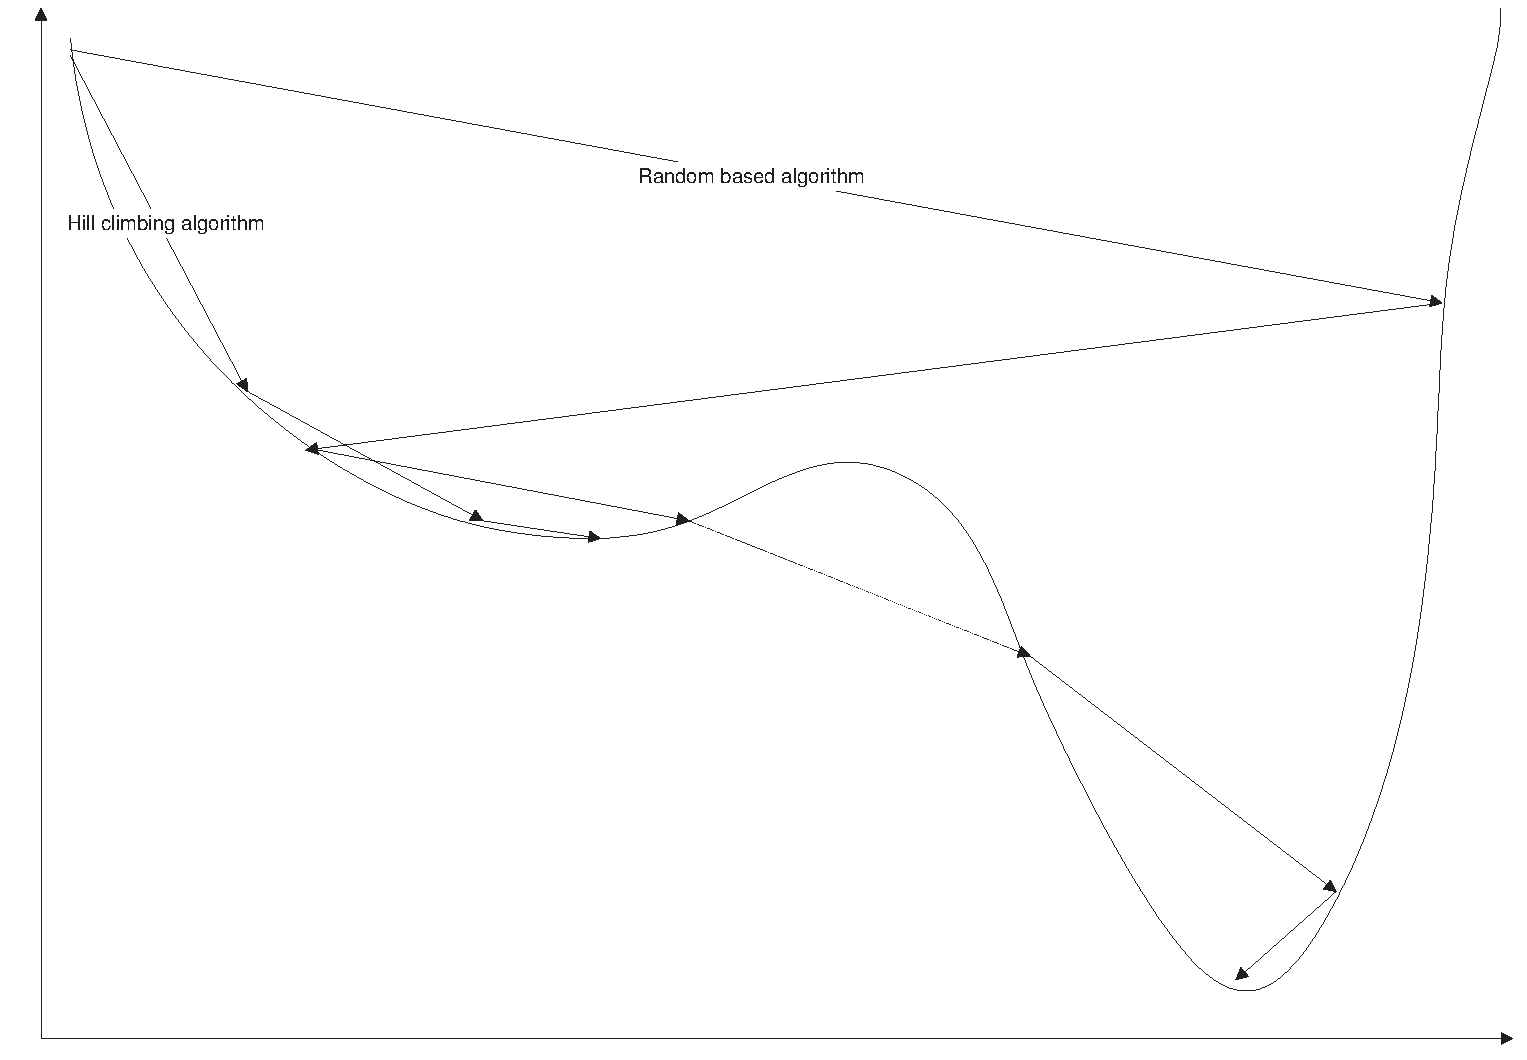
\includegraphics[width=12cm]{Figures/OptimizingComparisonvsd}
\caption{Compared behavior of hill climbing and random based algorithms.}\label{fig:hillvsrandom}
\end{figure}
After reading the above summary of the pro and cons of each
algorithm, the reader may have already come to the conclusion that
mixing the three algorithms together can make a very efficient
strategy to find the optimum of a wide variety of functions.

One can start with a genetic optimizer for a sufficient number of
iterations. This should ensure that the best points found at the
end of the search does not lie too far from the absolute optimum.
Then, one can use the simplex algorithm to get rapidly near the
optimum. The final location of the optimum is obtained using a
hill climbing optimizer.

\subsection{Multiple strategy approach --- General implementation}
This multiple strategy approach, inspired from the program MINUIT,
has been adapted to the use of the algorithms discussed here. The
class {\tt MultiVariableGeneralOptimizer} combines the three
algorithms: genetic, simplex and hill climbing, in this order. We
could have make it a subclass of {\tt Object}, but we decided to
reuse all the management provided by the abstract optimizer class
discussed in section \ref{sec:goptonedim}. Therefore, our general
purpose optimizer is a subclass of the abstract optimizer class
although it does not really uses the framework of an iterative
process. We only need one additional instance variable: the range
used to construct the hypercube search space for the vector
genetic chromosome manager. A corresponding setting method is
provided: {\tt setRange}.

The method {\tt initializeIterations} performs search using the
genetic algorithm as an option and, then, the simplex algorithm.
Since the genetic algorithm require a great deal of function
evaluate --- due to its stochastic nature --- it is a good idea to
give the user the choice of by-passing the use of the genetic
algorithm. If no range has been defined, only the simplex
algorithm is used from the supplied initial value. Otherwise a
search is made with the genetic algorithm using the initial value
and the range to define the search space. Then the simplex
algorithm is started from the best point found by the genetic
algorithm. The precision for the simplex search is set to the
square root of the precision for the final search. Less precision
is required for this step because the final search will give a
better precision.

The method {\tt evaluateIteration} performs the hill climbing
algorithm and returns it precision. As the desired precision of
the hill climbing algorithm is set to that of the general purpose
optimizer. As a consequence, there will only be a single
iteration.

Listing \ref{ls:optimizergeneral} shows the implementation in
Smalltalk. At this point we shall abstain from
commenting the code as the reader should have no more need for
such thing$\ldots$ Hopefully!

\marginpar{Figure \ref{fig:soptimizingclasses} with the box {\bf
MultiVariableGeneralOptimizer} grayed.}
\begin{listing} Smalltalk
implementation of a general optimizer \label{ls:optimizergeneral}
$$\halign{ #\hfil&\quad#\hfil\cr {\sl Class}& {\Large\bf DhbMultiVariableGeneralOptimizer}\cr
{\sl Subclass of }&{\tt DhbFunctionOptimizer}\cr\noalign{\vskip 1ex}
}$$


Instance methods
{\parskip 1ex\par\noindent}
{\bf computeInitialValues}
\begin{verbatim}
    self range notNil
        ifTrue: [ self performGeneticOptimization].
    self performSimplexOptimization.
\end{verbatim}
{\bf evaluateIteration}
\begin{verbatim}
    | optimizer |
    optimizer := DhbHillClimbingOptimizer forOptimizer: self.
    optimizer desiredPrecision: desiredPrecision;
              maximumIterations: maximumIterations.
    result := optimizer evaluate.
    ^ optimizer precision
\end{verbatim}
{\bf origin}
\begin{verbatim}
    ^ result
\end{verbatim}
{\bf origin:} {\tt anArrayOrVector}
\begin{verbatim}
    result := anArrayOrVector.
\end{verbatim}
{\bf performGeneticOptimization}
\begin{verbatim}
    | optimizer manager |
    optimizer := DhbGeneticOptimizer forOptimizer: functionBlock.
    manager := DhbVectorChromosomeManager new: 100 mutation: 0.1 
                                                       crossover: 0.1.
    manager origin: self origin asVector; range: self range asVector.
    optimizer chromosomeManager: manager.
    result := optimizer evaluate.
\end{verbatim}
{\bf performSimplexOptimization}
\begin{verbatim}
    | optimizer manager |
    optimizer := DhbSimplexOptimizer forOptimizer: self.
    optimizer desiredPrecision: desiredPrecision sqrt;
              maximumIterations: maximumIterations;
              initialValue: result asVector.
    result := optimizer evaluate.
\end{verbatim}
{\bf range}
\begin{verbatim}
    ^ self bestPoints
\end{verbatim}
{\bf range:} {\tt anArrayOrVector}
\begin{verbatim}
    bestPoints := anArrayOrVector.
\end{verbatim}


\end{listing}

\ifx\wholebook\relax\else\end{document}\fi

%\input{DataMining}
%\appendix
%\input{FloatingPointSimulation}
%\input{SmalltalkPrimer}
%\input{Distributions}
%\input{CentralMoments}
%%\input{Cdrom}
\begin{thebibliography}{Abramovitz\thinspace$\&$\thinspace Stegun}

\bibitem[Abramovitz\thinspace$\&$\thinspace Stegun]{AbrSteg}
Milton Abramovitz and Irene A. Stegun, {\em Handbook of Mathematical Functions}, Dover publications, Inc., 1964.

\bibitem[Achtley\thinspace$\&$\thinspace Bryant]{AtchBry}
William R. Achtley and Edwin H. Bryant editors,
{\em Benchmark Papers in Systematic and Evolutionary Biology},
Vol. 1, Dowden, Hutchinson\thinspace$\&$\thinspace Ross, Inc.,
Stroudsburg, Pa.; distributed by Halsted Press [John
Wiley\thinspace$\&$\thinspace Sons, Inc.], New York, 1975.

\bibitem[Bass]{Bass}J. Bass, {\em Cours de Math�matiques}, Tome II, Masson, 1968.

\bibitem[Beck]{Beck}Kent Beck, {\em Smalltalk Best Practice Patterns}, Prentice
Hall, 1997.

\bibitem[Berry\thinspace$\&$\thinspace Linoff]{BerLin}
Michael J.A. Berry and Gordon Linoff, {\em Data mining for
marketing, sales and customer support}, John
Wiley\thinspace$\&$\thinspace Sons, Inc., 1997.

\bibitem[Cormen {\textit et al.}]{CorLeiRiv}
Thomas H. Cormen, Charles E. Leiserson and Ronald L. Rivest, {\em
Introduction to Algorithms}, McGraw-Hill, 1990.

\bibitem[Gamma {\textit et al.}]{GoF}
Erich Gamma, Richard Helm, Ralph Johnson and John Vlissides , {\em
Design Patterns}, Addison-Wesley, 1995.

\bibitem[Gullberg]{Gullberg} Jan Gullberg, {\em Mathematics From the Birth of the Numbers},
W.W. Norton\thinspace$\&$\thinspace Company, 1997.

\bibitem[Ifrah]{Ifrah}Georges Ifrah, {\em Histoire Universelle des Chiffres},
Robert Laffont, 1994.

\bibitem[Knuth 1]{Knuth1}Donald E. Knuth, {\em The Art of
Computer Programming} Vol. 1, Addison-Wesley, 1973.

\bibitem[Knuth 2]{Knuth2}Donald E. Knuth, {\em The Art of Computer Programming} Vol. 2,
Addison-Wesley, 1981.

\bibitem[Knuth 3]{Knuth3}Donald E. Knuth, {\em The Art of
Computer Programming} Vol. 3, Addison-Wesley, 1973.

\bibitem[Koza {\textit et al.}]{Koza}John R. Koza, Forrest H, Bennett III, David Andre and Martin A. Keane,
{\em Genetic Programming III}, Morgan Kaufmann, 1999.

\bibitem[Law\thinspace$\&$\thinspace Kelton]{LawKel}
Averill M. Law and W. David Kelton, {\em Simulation Modeling and
Analysis}, McGraw-Hill, 1982.

%\bibitem[Lin\thinspace$\&$\thinspace Lee]{LinLee}
%Chin-Teng Lin and C.S.
%George Lee, {\em Neural Fuzzy Systems}, Prentice Hall, 1996.

\bibitem[Phillips\thinspace$\&$\thinspace Taylor]{PhiTay}
G.M. Phillips and P.J. Taylor, {\em Theory and Applications of
Numerical Analysis}, Academic Press: London and New York, 1973.

\bibitem[Press {\textit et al.}]{Press}William H. Press, Saul A. Teukolsky, William T. Vetterling
and Brian P. Flannery, {\em Numerical recipes for C : the art of
scientific computing}, Cambridge University Press, 1992.

\bibitem[Alpert {\textit et al.}]{StDesPat}Sherman R. Alpert, Kyle Brown and Bobby Woolf,
{\em Design Pattern Smalltalk Companion}, Addison-Wesley, 1998.

\bibitem[Smith]{Smalltalk} David N. Smith,
{\em IBM Smalltalk, The language}, Addison-Wesley, 1995.

\bibitem[Flanagan]{Java} David Flanagan,
{\em Java in a nutshell}, O'Reilly, 1996.

\end{thebibliography}



%%%%%%%%%%%%%%%%%%%%%%%%%%%%%%%%%%%%%%%%%%%%%%%%%%%%%%%%%%%%%%%%%%%%%%
\clearpage
% \textlatin{\lipsum[2-7]}

\end{document}
